\documentclass[10pt]{memoir}
\setstocksize{220mm}{155mm} 	        
\settrimmedsize{220mm}{155mm}{*}	
\settypeblocksize{170mm}{116mm}{*}	
\setlrmargins{18mm}{*}{*}
\setulmargins{*}{*}{1.2}
%\setlength{\headheight}{5pt}%
\checkandfixthelayout[lines]
\linespread{1.16}
\flushbottom

%%% Hyphenation settings
\usepackage[htt]{hyphenat}
\hyphenation{he-lio-trope opos-sum}
\tracingparagraphs=1
%Hyphenation in Devanāgarī of the edition still missing? Probably this needs to be modified in babel-iast package? 

%%% babel
\usepackage[english]{babel}
\usepackage{babel-iast/babel-iast}

\babelfont[iast]{rm}[Renderer=Harfbuzz, Scale=1.3]{AdishilaSan}%AdishilaSan}
\babelfont[english]{rm}{Adobe Text Pro}

%%% more functionality
\PassOptionsToPackage{hyphens}{url}
\usepackage{hyperref}
\usepackage{pdflscape}
\usepackage{cleveref}
\usepackage{url}
\usepackage{cleveref}
\usepackage{microtype}
\usepackage{lineno}

%\usepackage{bigfoot}
%%% more functions
\usepackage[dvipsnames]{xcolor}
%\usepackage[para,perpage]{footmisc}

%%%für den Counter von Kapiteln und Sätzen! 
\newcommand{\uproman}[1]{\uppercase\expandafter{\romannumeral#1}}
\newcommand{\lowroman}[1]{\romannumeral#1\relax}

\makeindex
\newfontfamily\sanskritfont[Script=Devanagari,Mapping=RomDev,Scale=1.1]{Sanskrit2003}
\usepackage{pifont,fourier-orns,lettrine,psvectorian,paralist,enumitem,pdfpages,wrapfig,tabulary,lettrine,longtable}
\setlist[enumerate]{itemsep=0mm}
\usepackage[autostyle]{csquotes}
\usepackage[defaultlines=2,all]{nowidow}
\usepackage{ellipsis,adforn,booktabs,longtable,url,tikz}
\lineskiplimit=-3pt          

\makechapterstyle{IeT}{%
  \chapterstyle{default}
  \renewcommand*{\printchapternonum}{\centering}
  \renewcommand*{\clearforchapter}{\cleartorecto} 
  \aliaspagestyle{chapter}{empty}}
\chapterstyle{IeT}
\setsecnumdepth{none}  \openright  \nouppercaseheads
\settocdepth{subsubsection}

%%%% test better pagebreaks
%\def\fussy{%
%  \emergencystretch\z@
%  \tolerance 200%
%  \hfuzz .1\p@
%  \vfuzz\hfuzz}

%\interfootnotelinepenalty=10000\relax

%\usepackage[maxfloats=256]{morefloats}

%\maxdeadcycles=500

%raggedbottomsectiontrue
%%\checkandfixthelayout


%%%%%%%  biblatex
%\newcommand{\noun}[1]{\textsc{#1}}    %  philosophy-verbose
\usepackage[backend=biber, sorting=nyt, style=verbose]{biblatex} %%%%ORIGINAL TiE
\renewcommand*{\mkbibnamefamily}[1]{\textsc{#1}}


\DeclareFieldFormat{url}{%
  \mkbibacro{URL}\addcolon\space
  \href{#1}{\nolinkurl{\thefield{urlraw}}}}

\DeclareFieldFormat{citeurl}{%
  \href{#1}{\nolinkurl{\thefield{urlraw}}}} 


\DeclareFieldFormat{postnote}{#1}
\renewcommand{\postnotedelim}{, }
\addbibresource{bindu.bib}

%%% ekdosis
\usepackage[teiexport=tidy,parnotes=true]{ekdosis}% =tidy cleans up HTML and XML documents by fixing markup errors and upgrading legacy code to modern standards. parnotes=footnotes below or above critical apparatus

\SetLineation{lineation=page, modulo} %lineation=page sets thenumbering to start afresh at the top of each page. =modulo makes every fifth line numbered. {lineation=page} makes every line numbered! 

\renewcommand{\linenumberfont}{\selectlanguage{english}\footnotesize} %sets language of lines to English

\SetTEIxmlExport{autopar=false} %autopar=falseinstructs ekdosis to ignore blank lines in the.tex sourcefile as markers for paragraph boundaries. As a result, each paragraph of the edition must be found within an environment associated with the xml <p> element

\SetHooks{
  lemmastyle=\bfseries,
  %refnumstyle=\selectlanguage{english}\bfseries,
  refnumstyle=\selectlanguage{english}\color{blue}\bfseries,
  appheight=0.8\textheight,
}

\newif\ifinapparatus
\DeclareApparatus{source}[
%bhook=\inapparatustrue,
lang=english,
notelang=english,
% bhook=\selectlanguage{english},
bhook=\selectlanguage{english}\textbf{Sources:},%
%maxentries=4, 
%ehook=.]
%sep={] },
%nosep,
]

\newif\ifinapparatus
\DeclareApparatus{testium}[
%bhook=\inapparatustrue,
lang=english,
notelang=english,
% bhook=\selectlanguage{english},
bhook=\selectlanguage{english}\textbf{Testimonia:},
%maxentries=4, 
%ehook=.]
%nosep, 
]

% Declare \ifinapparatus and set \inapparatustrue at the beginning of
% the apparatus criticus block. Also set the language.  
\newif\ifinapparatus
  \DeclareApparatus{default}[
  %bhook=\inapparatustrue, 
  lang=english,
  %maxentries=33,
  %bhook=\selectlanguage{english},
  sep = {] },
  delim=\hskip 0.75em,
  rule=\rule{0.7in}{0.4pt},
]

\newif\ifinapparatus
\DeclareApparatus{philcomm}[
%bhook=\inapparatustrue,
lang=english,
notelang=english,
bhook=\selectlanguage{english}\textbf{Philological Commentary:},
%bhook=\selectlanguage{english},
sep={: },
]

\ekdsetup{
showpagebreaks,
spbmk = \textcolor{blue}{spb},
hpbmk = \textcolor{red}{hpb}
}

%\usepackage{fnpos}
%\makeFNmid
%\makeFNbottom
\usepackage[bottom]{footmisc}
%%%%%%%%%%%%%%%%%%%%%%%%%%%
\makeatletter
\def\blfootnote{\gdef\@thefnmark{}\@footnotetext}
\makeatother
%%%%%%%%%%%%%%%%%%%%%%%%%


% Macros and Definitions for the Print of Sigla
\def\acpc#1#2#3{{#1}\rlap{\textrm{\textsuperscript{#3}}}\textsubscript{\textrm{#2}}\space}
\def\sigl#1#2{{{#1}}\textsubscript{\textrm{#2}}}
\def\None{{\sigl{N}{1}}} \def\Noneac{\acpc{N}{1}{ac}\,} \def\Nonepc{\acpc{N}{1}{pc}\,}
\def\Ntwo{{\sigl{N}{2}}} \def\Noneac{\acpc{N}{2}{ac}\,} \def\Nonepc{\acpc{N}{2}{pc}\,}
\def\Done{{\sigl{D}{1}}} \def\Doneac{\acpc{D}{1}{ac}\,} \def\Donepc{\acpc{D}{1}{pc}\,}
\def\Dtwo{{\sigl{D}{2}}} \def\Dtwoac{\acpc{D}{2}{ac}\,} \def\Dtwopc{\acpc{D}{2}{pc}\,}
\def\Uone{{\sigl{U}{1}}} \def\Uoneac{\acpc{U}{1}{ac}\,} \def\Uonepc{\acpc{U}{1}{pc}\,}                 
\def\Utwo{{\sigl{U}{2}}} \def\Utwoac{\acpc{U}{2}{ac}\,} \def\Utwopc{\acpc{U}{2}{pc}\,}

%%%%%%%%%%%%%% Tattvabinduyoga - List of Witnesses   %%%%%%%%%%%%%%%%%%%
\DeclareWitness{ceteri}{\selectlanguage{english}cett.}{ceteri}[]   
\DeclareWitness{E}{\selectlanguage{english}E}{Printed Edition}[]    
\DeclareWitness{P}{\selectlanguage{english}P}{Pune BORI 664}[]  
\DeclareWitness{B}{\selectlanguage{english}B}{Bodleian 485}[]       
\DeclareWitness{N1}{\selectlanguage{english}N\textsubscript{1}}{NGMPP 38/31}[]
\DeclareWitness{N2}{\selectlanguage{english}N\textsubscript{2}}{NGMPP B 38/35}[]
\DeclareWitness{L}{\selectlanguage{english}L}{LALCHAND 5876}[]  
\DeclareWitness{D}{\selectlanguage{english}D}{IGNCA 30019}[] 
%\DeclareWitness{D2}{\selectlanguage{english}D\textsubscript{2}}{IGNCA 30020}[]  
\DeclareWitness{U1}{\selectlanguage{english}U\textsubscript{1}}{SORI 1574}[] 
\DeclareWitness{U2}{\selectlanguage{english}U\textsubscript{2}}{SORI 6082}[]
%%%%%%%%%%%%%% Tattvabinduyoga - Groups of Witnesses   %%%%%%%%%%%%%%%%%%%
\DeclareWitness{X}{\selectlanguage{english}\alpha}{Alpha Group: D,N1,N2,U1}[]
\DeclareWitness{Y}{\selectlanguage{english}\beta}{Beta Group: B,E,L,P,U2}[]
%%%%%%%%%%%%% Testimonia
\DeclareWitness{Ysv}{\selectlanguage{english}Ysv}{Yogasvarodaya}[] %%%add infos!  

%%%%%%%%%%%%%%%%%%%%%%%%%%%%%%%%%%%%%%%%%%%
% Macro for Editing Abbrevs.
\def\om{\textrm{\footnotesize \textit{om.}\ }} %prints om. for omitted in apparatus
\def\korr{\textrm{\footnotesize \textit{em.}\ }} %prints em. for emended in apparatus
\def\conj{\textrm{\footnotesize \textit{conj.}\ }} %prints conj. for conjectured in apparatus

% \supplied{text} EDITORIAL ADDITION -> Within \lem oder \rdg
% \surplus{text} EDITORIAL DELETION -> Within \lem oder \rdg
% \sic{text} CRUX
% \gap{text} LACUNAE -> [reason=??, unit=??, quantity=??, extent=??]


%%%%%%%%%%%%%%%%%%%%%%%%%%%%%%%%%%%%%%%%%%% All macros of this list can be used in 
% Macro for Editing Abbrevs.
\def\eyeskip{\textrm{{ab.\,oc. }}}
\def\aberratio{\textrm{{ab.\,oc. }}}
\def\ad{\textrm{{ad}}}
\def\add{\textrm{{add.\ }}}
\def\ann{\textrm{{ann.\ }}}
\def\ante{\textrm{{ante }}} 
\def\post{\textrm{{post }}}
%\def\ceteri{cett.\,}                   
\def\codd{\textrm{{codd.\ }}}

\def\coni{\textrm{{coni.\ }}}
\def\contin{\textrm{{contin.\ }}}
\def\corr{\textrm{{corr.\ }}}
\def\del{\textrm{{del.\ }}}
\def\dub{\textrm{{ dub.\ }}}

\def\expl{\textrm{{explic.\ }}} 
\def\explica t{\textrm{{explic.\ }}}
\def\fol{\textrm{{fol.\ }}}
\def\foll{\textrm{{foll.\ }}}
\def\gloss{\textrm{{glossa ad }}}
\def\ins{\textrm{{ins.\ }}}      
\def\inseruit{\textrm{{ins.\ }}} 
\def\im{{\kern-.7pt\lower-1ex\hbox{\textrm{\tiny{\emph{i.m.}}}\kern0pt}}} %\textrm{\scriptsize{i.m.\ }}}      
\def\inmargine{{\kern-.7pt\lower-.7ex\hbox{\textrm{\tiny{\emph{i.m.}}}\kern0pt}}}%\textrm{\scriptsize{i.m.\ }}}      
\def\intextu{{\kern-.7pt\lower-.95ex\hbox{\textrm{\tiny{\emph{i.t.}}}\kern0pt}}}%\textrm{\scriptsize{i.t.\ }}}           
\def\indist{\textrm{{indis.\ }}}  
\def\indis{\textrm{{indis.\ }}}
\def\iteravit{\textrm{{iter.\ }}} 
\def\iter{\textrm{{iter.\ }}}
\def\lectio{\textrm{{lect.\ }}}   
\def\lec{\textrm{{lect.\ }}}
\def\leginequit{\textrm{{l.n. }}} 
\def\legn{\textrm{{l.n. }}}
\def\illeg{\textrm{{l.n. }}}

\def\primman{\textrm{{pr.m.}}}
\def\prob{\textrm{{prob.}}}
\def\rep{\textrm{{repetitio }}}
\def\secundamanu{\textrm{\scriptsize{s.m.}}}            \def\secm{{\kern-.6pt\lower-.91ex\hbox{\textrm{\tiny{\emph{s.m.}}}\kern0pt}}}%   \textrm{\scriptsize{s.m.}}}
\def\sequentia{\textrm{{seq.\,inv.\ }}}  
\def\seqinv{\textrm{{seq.\,inv.\ }}}
\def\order{\textrm{{seq.\,inv.\ }}}
\def\supralineam{{\kern-.7pt\lower-.91ex\hbox{\textrm{\tiny{\emph{s.l.}}}\kern0pt}}} %\textrm{\scriptsize{s.l.}}}
\def\interlineam{{\kern-.7pt\lower-.91ex\hbox{\textrm{\tiny{\emph{s.l.}}}\kern0pt}}}   %\textrm{\scriptsize{s.l.}}}
\def\vl{\textrm{v.l.}}   \def\varlec{\textrm{v.l.}} \def\varialectio{\textrm{v.l.}}
\def\vide{\textrm{{cf.\ }}}
\def\cf{\textrm{{cf.\ }}} 
\def\videtur{\textrm{{vid.\,ut}}}
\def\crux{\textup{[\ldots]} }
\def\cruxx{\textup{[\ldots]}}
\def\unm{\textit{unm.}}
%%%%%%%%%%%%%%%%%%%%%%%%%%%%%%%%%%%%

% List of Scholars
\DeclareScholar{ego}{ego}[
forename=Nils Jacob,
surname=Liersch]

% Persons:14\DeclareScholar{ego}{ego}[15forename=Robert,16surname=Alessi]17% Useful shorthands:18\DeclareShorthand{codd}{codd.}{V,I,R,H}19\DeclareShorthand{edd}{edd.}{Lit,Erm,Sm}20\DeclareShorthand{egoscr}{\emph{scripsi}}{ego}

%Useful shorthands:
%\DeclareShorthand{codd}{codd.}{V,I,R,H}
%\DeclareShorthand{edd}{edd.}{Lit,Erm,Sm}
\DeclareShorthand{egoscr}{em.}{ego}
\DeclareShorthand{egoscrconj}{conj.}{ego}
\DeclareShorthand{egomute}{\unskip}{ego}

\usepackage{xparse}

\NewDocumentEnvironment{tlg}{O{}O{}}{\setlength{\leftskip}{0pt}\vspace{-1ex}\begin{quotation}}{\hfill #1\ \vspace{-1ex}\end{quotation}\vspace{-1ex}} %verse environment
%\NewDocumentEnvironment{tlg}{O{}O{}}{\begin{verse}}{॥#1\hskip-4pt ॥\\ \end{verse}}
\NewDocumentCommand{\tl}{m}{{\selectlanguage{iast} #1}}

\NewDocumentCommand{\extra}{m}{{\textcolor{gray}{#1}}} %command for additions to U2
\NewDocumentCommand{\crazy}{m}{{\textcolor{red}{#1}}} %totally corrupted passage
\NewDocumentCommand{\coro}{m}{{\textcolor{violet}{#1}}} %colour for sentence counter! 

\NewDocumentEnvironment{prose}{O{}}{\begin{otherlanguage}{iast}}{\end{otherlanguage}}
% \NewDocumentEnvironment{padd}{O{}}{\begin{otherlanguage}{iast}}{\end{otherlanguage}}
\NewDocumentEnvironment{tlate}{O{}}
%\NewDocumentEnvironment{tadd}{O{}}

%Define two commands: \skp ("sanskrit plus"), to be ignored by TeX in
%the edition text, but processed in the TEI output. Conversely, \skm
%("sanskrit minus") is to be processed in the edition text, but
%ignored if found in the apparatus criticus and in the TEI output:

\NewDocumentCommand{\skp}{m}{}
\TeXtoTEIPat{\skp {#1}}{#1}

%\NewDocumentCommand{\skpp}{m}{}
%\TeXtoTEIPat{\skpp {#1}}{#1}

\NewDocumentCommand{\skm}{m}{\unless\ifinapparatus#1-\fi}
\TeXtoTEIPat{\skm {#1}}{}

% \NewDocumentCommand{\dd}{}{/\hskip-4pt/}
\NewDocumentCommand{\dd}{}{\mbox{/\hskip-4pt/}}
\TeXtoTEIPat{\dd {}}{//}


%%% modify environments and commands
%%% TEI mapping
\TeXtoTEIPat{\begin {tlg}}{<lg>} %lg=(Group of verse (s)) contains one or more verses or lines of verse that together form a formal unit (e.g. stanza, chorus).
\TeXtoTEIPat{\end {tlg}}{</lg>}

\TeXtoTEIPat{\begin {prose}}{<p>}
\TeXtoTEIPat{\end {prose}}{</p>}

\TeXtoTEIPat{\begin {tlate}}{<p>}
\TeXtoTEIPat{\end {tlate}}{</p>}

\TeXtoTEIPat{\\}{}
\TeXtoTEIPat{\linebreak}{<br/>}
\TeXtoTEIPat{\noindent}{}
%\TeXtoTEI{tl}{l}
\TeXtoTEI{emph}{hi}
\TeXtoTEI{bigskip}{}
\TeXtoTEI{None}{N1}
\TeXtoTEI{Ntwo}{N2}
\TeXtoTEI{Done}{D1}
\TeXtoTEI{Dtwo}{D2}
\TeXtoTEI{Uone}{U1}
\TeXtoTEI{Utwo}{U2}
%\TeXtoTEIPat{/}{ |}
%\TeXtoTEI{//}{ ||}
\TeXtoTEIPat{\korr}{em. }
\TeXtoTEIPat{\conj}{conj.}
\TeXtoTEIPat{\om}{om.}
\TeXtoTEIPat{english}{}
\TeXtoTEIPat{\hskip}{}
\TeXtoTEIPat{\hskip-4pt}{}
\TeXtoTEIPat{\hskip-2pt}{}
\TeXtoTEIPat{-}{ }
\TeXtoTEIPat{4pt}{}
\TeXtoTEIPat{2pt}{}
\TeXtoTEIPat{\textcolor {#1}{#2}}{<hi rend="#1">#2</hi>} 

% Nullify \selectlanguage in TEI as it has been used in
% \DeclareWitness but should be ignored in TEI.
\TeXtoTEI{selectlanguage}{}



\author{Nils Jacob Liersch}
\begin{document}
\cleardoublepage
%%%%%%%%%%%%%%%%%%%%%%%%%%%%%%%%%%%%%%%%%%
%%%%%%%%%%%%%%%%%%%%%%%%%%%%%%%%%%%%%%%%%% 
%%%%%%%%PAGEBREAK%%%%%%%PAGEBREAK%%%%%%%%%
%%%%%%%%%%%%%%%%%%%%%%%%%%%%%%%%%%%%%%%%%% 
%%%%%%%%%%%%%%%%PAGEBREAK%%%%%%%%%%%%%%%%%
%%%%%%%%%%%%%%%%%%%%%%%%%%%%%%%%%%%%%%%%%% 
%%%%%%%%PAGEBREAK%%%%%%%PAGEBREAK%%%%%%%%%
%%%%%%%%%%%%%%%%%%%%%%%%%%%%%%%%%%%%%%%%%% 
%%%%%%%%%%%%%%%%%%%%%%%%%%%%%%%%%%%%%%%%%% 
%%%%%%%%%%%%%%%%%%%%%%%%%%%%%%%%%%%%%%%%%% 
%%%%%%%%%%%%%%%%%%%%%%%%%%%%%%%%%%%%%%%%%% 
%%%%%%%%PAGEBREAK%%%%%%%PAGEBREAK%%%%%%%%%
%%%%%%%%%%%%%%%%%%%%%%%%%%%%%%%%%%%%%%%%%% 
%%%%%%%%%%%%%%%%PAGEBREAK%%%%%%%%%%%%%%%%%
%%%%%%%%%%%%%%%%%%%%%%%%%%%%%%%%%%%%%%%%%% 
%%%%%%%%PAGEBREAK%%%%%%%PAGEBREAK%%%%%%%%%
%%%%%%%%%%%%%%%%%%%%%%%%%%%%%%%%%%%%%%%%%% 
%%%%%%%%%%%%%%%%%%%%%%%%%%%%%%%%%%%%%%%%%% 
%%%%%%%%%%%%%%%%%%%%%%%%%%%%%%%%%%%%%%%%%% 
%%%%%%%%%%%%%%%%%%%%%%%%%%%%%%%%%%%%%%%%%% 
%%%%%%%%PAGEBREAK%%%%%%%PAGEBREAK%%%%%%%%%
%%%%%%%%%%%%%%%%%%%%%%%%%%%%%%%%%%%%%%%%%% 
%%%%%%%%%%%%%%%%PAGEBREAK%%%%%%%%%%%%%%%%%
%%%%%%%%%%%%%%%%%%%%%%%%%%%%%%%%%%%%%%%%%% 
%%%%%%%%PAGEBREAK%%%%%%%PAGEBREAK%%%%%%%%%
%%%%%%%%%%%%%%%%%%%%%%%%%%%%%%%%%%%%%%%%%% 
%%%%%%%%%%%%%%%%%%%%%%%%%%%%%%%%%%%%%%%%%% 
\begin{alignment}[
  texts=edition[class="edition"];
  translation[class="translation"],
  ]
  \begin{edition}
    \ekddiv{type=ed}
    \begin{prose}
      \noindent
%-----------------------------
%caturthaṃ liṃgādhāraṃ   tanmadhye/ liṃgasaṃkocanābhyāsāt  paścimadaṇḍamadhye prajñā nāḍī bhavati/  tanmadhye punar abhyāsakaraṇān manaḥ pavanayoḥ saṃcāro bhavati/ \E
%caturthaṃ liṃgādhāraṃ   tanmadhye  liṃgasaṃkocanābhyāsāt  paścīmadaṇḍamadhye vajñā nāḍī  bhavati   tanmadhye punar abhyāsakaraṇān manaḥ pavanayoḥ saṃcāro bhavati \P
%caturtha--liṃgādhāraṃ   tanmadhye  liṃgasaṃkocanābhyāsāt  paścīmadaṇḍamadhye vajñā nāḍī  bhavatī/  tanmadhye punar abhyāsakaraṇāt punaḥ pavanayo  saṃcāro bhavatī/     \B
%caturtha--liṃgādhāraṃ// tanmadhye  liṃgasaṃkocanābhyāsāt  paścamadaṇḍamadhye vajñā nāḍī  bhavatī// tanmadhye punar abhyāsakaraṇāt punaḥ pavanayo  saṃcāro bhavatī//     \L %%%%%%%%%%%20.jpg
%caturthaṃ liṃgādhāraṃ   tanmadhye/ liṃgasaṃkocanābhyāsāt/ paścimadaṇḍamadhye vajranāḍī   bhavati/  tanmadhye punaḥ abhyāsakaraṇāt manaḥpavanayoḥ saṃcāro bhavati/ \N1
%caturtha--liṃgādhāraṃ// tanmadhye/ liṃgasaṃkocanābhyāsāt//paścimadaṇḍamadhye vajrānāḍī   bhavati// tanmadhye punaḥ abhyāsakaraṇāt manaḥpavanayoḥ saṃcoro bhavati// \D
%caturthaṃ liṃgādhāraṃ   tanmadhye  liṃgasakoṇābhyāsāt//   paścimadaṇḍamadhye vajranāḍī   bhavati/  tanmadhye punar ābhyāsakaraṇāt manaḥpavanayoḥ saṃcāro bhavati// \N2
%caturthaṃ liṃgādhāraṃ   tanmadhye  liṃgasaṃkocanābhyāsāt  paścimadaṇḍamadhye vajranāḍī   bhavati   tanmadhye punar ābhyāsakaraṇāt manaḥpavanayoḥ saṃcāro bhavati    \U1    %%%283.jpg
%caturthaṃ liṃgādhāraṃ   tanmadhye  liṃgasaṃkocanābhyāsāt  paścimadaṇḍamadhye vajranāḍī   bhavati   tanmadhye punar ābhyāsakaraṇān manaḥpavanayoḥ saṃcāro bhavati//   \U2
%-----------------------------
%The fourth is the penis support. Due to the execution of repeated practice of contracting the penis in the centre of it, the adamantine channel appears in the middle of the staff of the back. From the repeated practice again [and again] the transition of both breath and mind into its center arises.  
%-----------------------------
      \note[type=source, labelb=220, labele=_220e, nosep]{cf. Ysv (PT pp. 839-840): liṅgādhāraṃ caturthan tu liṅgasaṅkocanan tu ca | liṅgasaṅkocanābhyāsāt paścimādaṇḍamadhyagaḥ | vajranāḍīti (\textit{vajrānāḍī tu} YK 2.20) tanmadhye punar abhyasayaṃs (\textit{abhyasanan} YK 2.20) tathā | sañcāro vāyumanasor atisañcāra iti (\textit{ratiṃ sañcarati} YK 2.20) tridhā | granthitrayavibhedas (\textit{°bhedan} YK 2.21) tu tadbhedo brahmamārgataḥ | brahmapadmo (\textit{°padme} YK 2.21) vāyupūrṇo (\textit{°pūrṇe} YK 2.21) bhūtvā tiṣṭhati yogirāṭ | vīryastambho bhavet tena sādhayet tu sadā yuvā | mūlādhāre brahmapadme ṣaṭpadme ca tathā tathā |}
      \note[type=source, labelb=219, labele=_220e, nosep]{cf. SSP 2.13 (Ed. pp. 33-34): caturtho meḍhrādhāraḥ | liṅgasaṃkocanena brahmagranthitrayaṃ bhitvā bhramaraguhāyāṃ viśramya tata ūrdhvamukhe bindustambhanaṃ bhavati| eṣā vajrolī prasiddhā}
\app{\lem[wit={ceteri}]{caturthaṃ}
  \rdg[wit={B,D,L}]{caturtha°}}
liṅgādhāraṃ/
tanmadhye
liṅga\app{\lem[wit={ceteri},alt={saṃkocanā°}]{saṃkocanā}
  \rdg[wit={N2}]{sakoṇā°}
}bhyāsā\skp{t-pa}
\app{\lem[wit={ceteri}, alt={paścima°}]{\skp{t-pa}paścima}
  \rdg[wit={B,P}]{paścīma°}
  \rdg[wit={L}]{paścama°}
}daṇḍamadhye
\app{\lem[wit={ceteri}, alt={vajra°}]{vajra}
  \rdg[wit={B,P,L}]{vajñā°}
  \rdg[wit={E}]{prajñā°}
}nāḍī
\app{\lem[wit={ceteri}]{bhavati}
  \rdg[wit={B,L}]{bhavatī}}/
tanmadhye punar-ābhyāsa\app{\lem[wit={E,P,U2}, alt={°karaṇān}]{karaṇā\skp{n-ma}}
  \rdg[wit={ceteri}]{karaṇāt}
}\app{\lem[wit={ceteri}, alt={manaḥ}]{\skm{n-ma}naḥ}
  \rdg[wit={B,L}]{punaḥ}}
\app{\lem[wit={ceteri}]{pavanayoḥ}
  \rdg[wit={B,L}]{pavanayo}}
\app{\lem[wit={ceteri}]{saṃcāro}
  \rdg[wit={D}]{saṃcoro}}
\app{\lem[wit={ceteri}]{bhavati}
  \rdg[wit={B,L}]{bhavatī}}/
%-----------------------------
%tayoḥ saṃcārān  madhye granthitrayaṃ truṭyati/   \E
%tayoḥ saṃcārān  madhye graṃthitrayaṃ truṭyati    \P
%tayo  saṃcārān  madhye granthitrayaṃ truṭyatī/   \B
%tayoḥ saṃcārān  madhye graṃthitrayaṃ truṭayatī   \L
%tayoḥ saṃcārān  madhye granthitrayaṃ truṭyati/   \N1 %truṭyati="zerbrechen"
%tayoḥ saṃcārāt  madhye graṃthitrayaṃ truṭyati//  \D 
%tayoḥ saṃcārān  madhye granthitrayaṃ ... ..ti/   \N2
%tayoḥ saṃccārāt madhye graṃthitrayaṃ trudyati    \U1
%tayoḥ saṃccārān madhye graṃthitrayaṃ truṭyati//  \U2
%-----------------------------
%Caused by the transition of them both into the center the trinity of knots breaks.
%-----------------------------
\app{\lem[wit={ceteri}]{tayoḥ}
  \rdg[wit={B}]{tayo}}
\app{\lem[wit={ceteri},alt={saṃcārān}]{saṃcārā\skp{n-ma}}
  \rdg[wit={D,U1}]{saṃcārāt}
}\skm{n-ma}dhye
granthitrayaṃ
\app{\lem[wit={ceteri}]{truṭyati}
  \rdg[wit={B}]{truṭyatī}
  \rdg[wit={L}]{truṭayatī}
  \rdg[wit={U1}]{trudyati}
  \rdg[wit={N2}]{ti}}/
%-----------------------------
% tatroṭanāt        pavano  brahmakamalamadhye pūrṇo bhūtvā tiṣṭhati/  \E
%                                                                      \P
% tatroṭanāt        pavano  brahmakamadhye     pūrṇā bhūtvā tiṣṭhati// \B
% tatroṭanāt        pavano  brahmakamadhye     pūrṇā bhūtvā tiṣṭhati// \L
% tattroṭanāt       pavanaḥ brahmakamalamadhye pūrṇo bhūtvā tiṣṭhati/  \N1 
% tata troṭanāt     pavanaḥ brahmakamalamadhye pūrṇo bhūtvā tiṣṭhati// \D 
% tata troṭanāt     pavanaḥ brahmakamalamadhye pūrṇo bhūtvā tiṣṭhati/  \N2
% tatroṭaṇāt        pavanaḥ brahmakamalamadhye pūrṇo bhūtvā tiṣṭhati   \U1
% tattroṭaṇāt       pavanaḥ brahmakamalamadhye pūrṇo bhūtvā tiṣṭhati// \U2
%-----------------------------
% There, from the breaking of that, the vitalwind, after having filled up (the central channel?) resides within the Brahma-lotus. 
%-----------------------------
\app{\lem[wit={N1,U2},alt={°tattroṭanāt}]{tattroṭanā\skp{t-pa}}
  \rdg[wit={B,E,L,U1}]{tatroṭanāt}
  \rdg[wit={D,N2}]{tata troṭanāt}
}\app{\lem[wit={B,E,L},alt={pavano}]{\skm{t-pa}vano}
  \rdg[wit={ceteri}]{pavanaḥ}}
brahma\app{\lem[wit={ceteri}, alt={°kamala°}]{kamala}
  \rdg[wit={B,L}]{°ka°}
}madhye
\app{\lem[wit={ceteri}]{pūrṇo}
  \rdg[wit={B,L}]{pūrṇā}}
bhūtvā tiṣṭhati/
%-----------------------------
% tato vīryastambho bhavati/  puruṣaḥ sadaiva   yuvā      bhavati/ \E
% tato vīryastaṃbho bhavati   puruṣaḥ saṃdaivaṃ yuve   prabhavati  \P
% tato vīryastambho bhavatī// puruṣaḥ sadaiva   yuvai     bhavatī/ \B
% tato vīryastaṃbho bhavati   puruṣaḥ sadaiva   yuvaiva   bhavati// \L
% tato vīryastambho bhavati/  puruṣaḥ sadaiva   yuvā/e va bhavati// \N1 %truṭyati="zerbrechen"
% tato vīryastambho bhavati// puruṣaḥ sadaiva   yuvaiva   bhavati// \D 
% tato vīryastambho bhavati/  puruṣa  sadaiva   yurvaiva  bhavati// \N2
% tato vīryastaṃbho bhavati/  puruṣaḥ sadaiva   yuvaivaṃ  bhavati \U1
% tato vīryastaṃbho bhavati   puruṣaḥ sadaiva   vaibhavo  bhavati// \U2
%-----------------------------
% From that virility and strength arise. The person becomes youthful forever.
%-----------------------------
tato vīryastambho bhavati/
\app{\lem[wit={ceteri}]{puruṣaḥ}
  \rdg[wit={N2}]{puruṣa}}
\app{\lem[wit={ceteri}]{sadaiva}
  \rdg[wit={P}]{saṃdaivaṃ}}
\app{\lem[wit={D,L}]{yuvaiva}
  \rdg[wit={E}]{yuvā}
  \rdg[wit={P}]{yuve}
  \rdg[wit={B}]{yuvai}
  \rdg[wit={N1}]{yuve va}
  \rdg[wit={N2}]{yurvaiva}
  \rdg[wit={U1}]{yuvaivaṃ}
  \rdg[wit={U2}]{yuvaivaṃ}}
\app{\lem[wit={ceteri}]{bhavati}
  \rdg[wit={B}]{bhavatī}
  \rdg[wit={P}]{prabhavati}}/\linelabel{_220e}
%-----------------------------
%paṃcama  udgīryāṇāṃ svādhiṣṭhānaṃ tatra bandhanān      malamūtrayor nāśo   bhavati/  \E
%paṃcamaṃ uḍḍīyāṇāṃ  svādhiṣṭhānaṃ tatra baṃdhadānān    malamūtrayor nāśo   bhavati   \P
%paṃcama  uḍḍiyānāṃ  svādhiṣṭhānaṃ tatra baṃdha dīyate/ malamūtrayor nāśo   bhavatī// \B
%paṃcamaṃ uḍḍiyānāṃ  svādhiṣṭhānaṃ tatra baṃdha dīyate/ mūlamūcayor  nāśo   bhavati// \L 
%paṃcamaṃ udyānaṃ                  tatra baṃdhanāt      malamūtrayor nāśe/o bhavati// \N1 [s.10, verso, z4]
%paṃcamaṃ udyāṇāṃ                  tatra vaṃdhanāt      malamūtrayor nāśo   bhavati// \D
%paṃcam   odyānaṃ                  tatra baṃdhanāt      malamūtrayor nāśo   bhavati/  \N2
%paṃcamaṃ uddyānaṃ                 tatra baṃdhadānāt    malamūtrayor nāśo   bhavati   \U1
%paṃcamaṃ uḍḍīyāṇaṃ  svādhiṣṭhānaṃ tatra badhadānān     malamūtrayor nāśo   bhavati// \U2
%-----------------------------
%The fifth is Udyāna. From performing \textit{bandha} there, urine and faeces disappear.  
%-----------------------------
\note[type=source, labelb=222, labele=_222e, nosep]{cf. YSv (PT p. 840): pañcamaṃ jaṭharādhāraṃ tadā bandhayati kramāt | mṛtyunā bhaṅgasiddho 'yaṃ (\textit{mṛtyunā māṅga°} YK 2.23) mṛtyor (\textit{mṛtyur} YK 2.23) eva kṣayaṅkaraḥ | anena paścimād ūrddhaṃ (\textit{ūrdhvaṃ} YK 2.24) vāyuḥ kuryād viśāladhīḥ | bandho 'yaṃ buddhimanasoḥ pañcamādhārakālajit |}
\note[type=source, labelb=221, labele=_222e, nosep]{cf. SSP 2.14 (Ed. p. 34): pañcame oḍīyāṇādhārayor bandhanān malamūtrasaṃkocanaṃ bhavati | *uḍyānā° etc. in various mss.}
\app{\lem[wit={ceteri}]{pañcamaṃ}
  \rdg[wit={B}]{paṃcama}
  \rdg[wit={N2}]{paṃcam}}
\app{\lem[wit={B,L}]{uḍḍiyānāṃ svādhiṣṭhānaṃ}
  \rdg[wit={P,U2}]{uḍḍīyāṇaṃ svādhiṣṭhānaṃ}
  \rdg[wit={D,N1}]{udyānaṃ}
  \rdg[wit={N2}]{odyānaṃ}
  \rdg[wit={U1}]{uddyānaṃ}
  \rdg[wit={P}]{uḍḍīyāṇāṃ svādhiṣṭhānaṃ}
  \rdg[wit={E}]{udgīryāṇāṃ svādhiṣṭhānaṃ}}/
\note[type=philcomm, labelb=223, lem={uḍḍīyāṇaṃ}]{Spellings for the \textit{pīṭha} named \textit{uḍḍīyāṇa} vary across yogic literature. \getsiglum{B}, \getsiglum{E}, \getsiglum{L}, \getsiglum{P}, \getsiglum{U2} add the expression \textit{svādhiṣṭhānaṃ} which was associated with the same \textit{pīṭha} in chapter \uproman{5}. l.1. I choose the most common spelling since, stemmatically, there is no preferable variant.}
tatra
\app{\lem[wit={E}]{bandhanā\skp{n-ma}}
  \rdg[wit={U2}]{badhadānān}
  \rdg[wit={N1,N2}]{baṃdhanāt}
  \rdg[wit={D}]{vaṃdhanāt}
  \rdg[wit={U1}]{baṃdhadānāt}
  \rdg[wit={P}]{baṃdhadānān}
  \rdg[wit={B,L}]{baṃdha dīyate}
}\app{\lem[wit={ceteri},alt={malamūtrayor}]{\skm{n-ma}lamūtrayo\skp{r-nā}}
  \rdg[wit={L}]{mūlamūcayor}
}\skm{r-nā}śo
\app{\lem[wit={ceteri}]{bhavati}
  \rdg[wit={B}]{bhavatī}}/\linelabel{_222e}
    \end{prose}
  \end{edition}
  \begin{translation}
    \ekddiv{type=trans}
    \begin{tlate}
      \noindent
      The fourth is the penis support. Due to the execution of repeated practice of contracting the penis in the centre of it, the adamantine channel\footnote{The adamantine channel (\textit{vajranāḍī}) is another synonym for the central channel. Rāmacandra adapted the term from the \textit{Yogasvarodaya}. \citetitle{yogatarangini} in the commentary on 1.13 uses the term \textit{vajragarbha}, ``the adamantine womb''.} appears in the middle of the staff of the back\footnote{The staff of the back (\textit{paścimadaṇḍa}) is the central channel, cf. \citetitle{peterson1888} 4365.}. From the repeated practice again [and again], both breath and mind move into its centre. Caused by the transition of both [breath and mind] into the centre [of the adamantine channel] the trinity of knots\footnote{The trinity of knots are: 1. the knot of Brahmā/Brahman (\textit{brahmagranthi}) usually situated in the lower regions of the body (cf. \citetitle{liersch2023} 23-24); 2. the knot of Viṣṇu (\textit{viṣṇugranthi}) at the level of the heart (cf. \citetitle{liersch2023} 25 and \citetitle{gsatacod} 80); and 3. the knot of Rudra (\textit{rudragranthi}) at the level of the head or between the eyebrows (cf. \citetitle{liersch2023} 25 and \citetitle{gsatacod} 81). Depending on text and tradition, it is either the breath (cf. \citetitle{asiddhi} 13.9-11) or the \textit{kuṇḍalinī} (cf. \citetitle{yogabija} 96-7 and \citetitle{gsatacod} 74-86) that enters the central channel and pierces the knots. It remains uncertain if knots are supposed to be something physical or mental. \citetitle{gsatacod} 48 states that the entrance to the central channel is blocked by phlegm (physical) and, in the same breath, mentions that the three knots have arisen from the three \textit{guṇa}s, which might be interpreted as physical or mental. Nevertheless, the three knots in yoga texts, in one way or another, obstruct the central passage.} breaks. There, from the breaking of that, the vital wind, after having filled up (the central channel?), resides within the lotus of Brahmā/Brahman\footnote{The lotus of Brahmā/Brahman refers to the eighth \textit{cakra} in Rāmacandra's system, cf. chapter \uproman{8}, p. \pageref{cakra8}. The same location is expressed in the \citetitle{ssplonavla} 2.13 and \citetitle{yogatarangini} commentary on 1.13 with the term ``buzzing hive'' (\textit{brahmaraguhā}) usually situated on top of the head (\citetitle{jogpradipyaka} 932; cf. \citetitle{peterson1888} 4366 and \citetitle{gorakbhani} 28.2 and 30.4).}. From that, virility and strength arise. The person becomes youthful forever.\footnote{Most of the consulted texts situate the fourth \textit{adhāra} at the penis (\textit{meḍhra}). \citetitle{sarada} and \citetitle{jyotsna} place the fourth support at the thighs (\textit{ūru}). \citetitle{shivayogapradipika} 3.20 and \citetitle{ssplonavla} 2.13 additionally associate the practice with the arrest of semen (\textit{bindustambha}). However, \citetitle{ssplonavla} calls this \textit{vajrolī}.} %However, just \citetitle{ssplonavla} calls this \textit{vajrolī}.}
      % Already in \citetitle{asiddhi} 31.2, the breath that has reached the \textit{brahmarandhra} is associated with the emergence of a particular sound. However, in this text, it is the tinkling sound of a lute (\textit{vīṇā}).
      
      The fifth is Uḍḍīyāna at the Svādiṣṭhāna[\textit{cakra}]\footnote{For a further discussion of the term \textit{uḍḍiyāṇa}, see p.\pageref{cakra2} fn. 23.}. From performing \textit{bandha} there, urine and faeces disappear.\footnote{\citetitle{shivayogapradipika}, \citetitle{ssplonavla} and \citetitle{yogatarangini} share the concept of performing a \textit{bandha} at the location of Uḍḍīyāna. \citetitle{hathatattvakaumudi} instructs to do a pressing (\textit{moṭana}) at the waist (\textit{kaṭau}). \textit{Netroddyota}, along with \citetitle{sarada} and \citetitle{jyotsna} situate the fifth \textit{adhāra} at the anus (\textit{pāyu} or \textit{sīvanī}), whereas the \textit{Yogasvarodaya} situates the fifth \textit{adhāra} at the belly (\textit{jaṭharādhāra}) and provides details (cf. sources) not reflected in Rāmacandra's text. This observation indicates that Rāmacandra relies more on the \citetitle{ssplonavla} at this point.}
\clearpage 
    \end{tlate}
  \end{translation}
\end{alignment}
\pagebreak %after pp. 73-74 
%%%%%%%%%%%%%%%%%%%%%%%%%%%%%%%%%%%%%%%%%%
%%%%%%%%%%%%%%%%%%%%%%%%%%%%%%%%%%%%%%%%%% 
%%%%%%%%PAGEBREAK%%%%%%%PAGEBREAK%%%%%%%%%
%%%%%%%%%%%%%%%%%%%%%%%%%%%%%%%%%%%%%%%%%% 
%%%%%%%%%%%%%%%%PAGEBREAK%%%%%%%%%%%%%%%%%
%%%%%%%%%%%%%%%%%%%%%%%%%%%%%%%%%%%%%%%%%% 
%%%%%%%%PAGEBREAK%%%%%%%PAGEBREAK%%%%%%%%%
%%%%%%%%%%%%%%%%%%%%%%%%%%%%%%%%%%%%%%%%%% 
%%%%%%%%%%%%%%%%%%%%%%%%%%%%%%%%%%%%%%%%%% 
%%%%%%%%%%%%%%%%%%%%%%%%%%%%%%%%%%%%%%%%%% 
%%%%%%%%%%%%%%%%%%%%%%%%%%%%%%%%%%%%%%%%%% 
%%%%%%%%PAGEBREAK%%%%%%%PAGEBREAK%%%%%%%%%
%%%%%%%%%%%%%%%%%%%%%%%%%%%%%%%%%%%%%%%%%% 
%%%%%%%%%%%%%%%%PAGEBREAK%%%%%%%%%%%%%%%%%
%%%%%%%%%%%%%%%%%%%%%%%%%%%%%%%%%%%%%%%%%% 
%%%%%%%%PAGEBREAK%%%%%%%PAGEBREAK%%%%%%%%%
%%%%%%%%%%%%%%%%%%%%%%%%%%%%%%%%%%%%%%%%%% 
%%%%%%%%%%%%%%%%%%%%%%%%%%%%%%%%%%%%%%%%%% 
%%%%%%%%%%%%%%%%%%%%%%%%%%%%%%%%%%%%%%%%%% 
%%%%%%%%%%%%%%%%%%%%%%%%%%%%%%%%%%%%%%%%%% 
%%%%%%%%PAGEBREAK%%%%%%%PAGEBREAK%%%%%%%%%
%%%%%%%%%%%%%%%%%%%%%%%%%%%%%%%%%%%%%%%%%% 
%%%%%%%%%%%%%%%%PAGEBREAK%%%%%%%%%%%%%%%%%
%%%%%%%%%%%%%%%%%%%%%%%%%%%%%%%%%%%%%%%%%% 
%%%%%%%%PAGEBREAK%%%%%%%PAGEBREAK%%%%%%%%%
%%%%%%%%%%%%%%%%%%%%%%%%%%%%%%%%%%%%%%%%%% 
%%%%%%%%%%%%%%%%%%%%%%%%%%%%%%%%%%%%%%%%%% 
\begin{alignment}[
  texts=edition[class="edition"];
  translation[class="translation"],
  ]
  \begin{edition}
    \ekddiv{type=ed}
    \begin{prose}
      \noindent
%-----------------------------
%ṣaṣṭho nābhyādhāraḥ/    \E
%ṣaṣṭho nābhyādhāraḥ   tatra         prāṇavābhyāsād  nāhato   nāraḥ   svayam utpadyate / \P
%ṣaṣṭho nābhyādhāraḥ   tatra         prāṇavābhyāsād  anāhato  nādaḥ// svayam utpadyate// \B
%ṣaṣṭho nābhyādhāraḥ   tatra         prāṇavābhyāsād  anāhato  nādaḥ// svayam utpadyate... \L 
%ṣaṣṭho nābhyādhāraḥ/  tatra         praṇavābhyāsāt  anāhato  nādaḥ   svayam ūtpadyate/  \N1
%ṣaṣṭho nābhyādhāraḥ// tatra         prāṇavābhyāsāt  anāhato  nādaḥ// svayam utpadyate// \D
%ṣaṣṭho nābhyādhāraḥ   tatra         praṇavābhyāsāt  anāhato  tādaḥ   svayaṃ utpadyate/ \N2
%ṣaṣṭho nābhyādhāras   tatra         praṇavābhyāṃsad ānāhato  nadaḥ   svayam utpadyate   \U1
%ṣaṣṭho nābhyādhāre//  tatra         prāṇavābhyāsād  anohato  nādaḥ   svayam utpadyate// \U2
%-----------------------------
%The sixth is the support of the navel. From repeated practice of \textit{praṇava}, the unstruck sound arises by itself. 
%-----------------------------
\note[type=source, labelb=225, labele=_225e, nosep]{cf. YSv (PT p. 840): nābhyādhāro bhavet ṣaṣṭhas (\textit{ṣaṣṭhaṃ} YK 2.25) tatra prāṇaṃ samabhyaset | svayam utpadyate nādo nādato muktidantataḥ (\textit{muktidaṇḍataḥ} YK 1.25) |}
\note[type=source, labelb=224, labele=_225e, nosep]{cf. SSP 2.15 (Ed. p. 34): ṣaṣṭhe nābhyādhāra oṃkāram ekacittenoccārayet | nādalayo bhavati |}
ṣaṣṭho
\app{\lem[wit={ceteri}]{nābhyādhāraḥ}
  \rdg[wit={U1}]{nābhyādhāras}
  \rdg[wit={U2}]{nābhyādhāre}}/
\app{\lem[wit={ceteri}]{tatra}
  \rdg[wit={E}]{\om}}
\app{\lem[wit={B,L,P,U2}]{prāṇavābhyāsā\skp{d-a}}
  \rdg[wit={D,N1,N2}]{prāṇavābhyāsā1}
  \rdg[wit={U1}]{prāṇavābhyāṃsad}
}\app{\lem[wit={ceteri},alt={°anāhato}]{\skm{d-a}nāhato}
    \rdg[wit={P}]{nāhato}
    \rdg[wit={U1}]{ānāhato}
    \rdg[wit={U2}]{anohato}}
  \app{\lem[wit={ceteri}]{nādaḥ}
    \rdg[wit={P}]{nāraḥ}
    \rdg[wit={N2}]{tādaḥ}}
  \app{\lem[wit={ceteri}]{svaya\skp{m-u}}
    \rdg[wit={N2}]{svayaṃ}
}\app{\lem[wit={ceteri},alt={utpadyate}]{\skm{m-u}tpadyate}
  \rdg[wit={N1}]{ūtpadyate}}/
\note[type=philcomm, labelb=225a, lem={tatra \ldots svayam utpadyate}]{Sentence omitted in \getsiglum{E}.}\linelabel{_225e}
%-----------------------------
%                             tasmin sthāne prāṇavāyor  nirodhāt            ṣaḍapi kamalāny ūrdhvamukhāni             vikasaṃti// \E                                                     
%saptamo hṛdayarūpadhāraḥ     tasmin sthāne prāṇavāyor  nirodhāt            ṣadapi kamalāny ūrdhvamukhāni             vikasaṃti  \P  %%%7653.jpg 
%                             tasmin sthāne prāṇavāyo   nirodhāt/           ṣaḍapi kamalāny ūrdhvamukhāni             vikasaṃti// \B
%saptamo hṛdayarūpadhāraḥ//   tasmin sthāne prāṇavāyor  nirodhāt            ṣadapi kamalāny ūrdhvamukhāni             vikasaṃti// \L
%saptamo hṛdayarūpa ādhāraḥ   tasmin sthāne prāṇavāyor  nirūṃdhanāt/        ṣadapi kamalāny ūrdhvamukhaṃ              vikasaṃti// \N1
%saptamo hṛdayarūpa ādhāraḥ// tasmin sthāne prāṇavāyor  nir???ūṃ???dhanāt// ṣadapi kamalāny ūrdhvamukhaṃ              vikasaṃti// \D
%saptamo hṛdayarūpādhāraḥ     tasmin sthāne prāṇavāyor  nirūṃdhanāt/        ṣadapi kamalāny ūrdhve mukhaṃ              vikasaṃti// \N2 %%%%%%%%%[S.9, recto, z.4]
%saptamo hṛdayarūpādhāraḥ     tasmin sthāne prāṇavāyor  nirūṃdhanāt         ṣadapi kamalāny ūrusyordha mukhaṃ bhavati vikasaṃti  \U1
%saptamo hṛdayādhāraḥ         tasmin sthāne prāṇavāyor  nirodhāt//          ṣadapi kamalāny ūrddhvamukhāni            vikasaṃti//  \U2
%-----------------------------
%The seventh is the support of the heart-form. From the restraint of the Prāṇa vitalwind in this location the six upward facing lotusses blossom.   
%-----------------------------
\note[type=source, labelb=226, labele=_226e, nosep]{cf. SSP 2.16 (Ed. p. 34): saptame hṛdayādhāre prāṇaṃ nirodhayet | kamalavikāso bhavati |}
\note[type=source, labelb=227, labele=_226e, nosep]{cf. YSv (PT p. 840): saptamo hṛdayādhāras tasmin vāyunibandhanāt | ūrddhaktrāṇi (\textit{ūrdhvavaktrāṇi} YK 2.26) padmāni vikasanti mahān bhavet |}
\app{\lem[wit={ceteri}]{saptamo}
  \rdg[wit={B,E}]{\om}}
\app{\lem[wit={ceteri}]{hṛdaya}
  \rdg[wit={U2}]{hṛdayā°}
  \rdg[wit={B,E}]{\om}
}\app{\lem[wit={N2,U1},alt={°rūpādhāraḥ}]{rūpādhāraḥ}
  \rdg[wit={L}]{°rūpadhāraḥ}
  \rdg[wit={D,N1}]{rūpa ādhāraḥ}
  \rdg[wit={U2}]{°dhāraḥ}
  \rdg[wit={B,E}]{\om}}/ 
tasmin-sthāne
\app{\lem[wit={ceteri},alt={prāṇavāyor}]{prāṇavāyo\skp{r-ni}}
  \rdg[wit={B}]{prāṇavāyo}
}\app{\lem[wit={Y},alt={nirodhāt}]{\skm{r-ni}rodhā\skp{t-ṣa}}
  \rdg[wit={X}]{nirūṃdhanāt}
}\app{\lem[wit={B,E},alt={ṣaḍ api}]{\skm{t-ṣa}ḍapi}
  \rdg[wit={ceteri}]{ṣadapi}}   
kamalā\skp{ny-ū}\app{\lem[wit={ceteri},alt={ūrdhvamukhāni}]{\skm{ny-ū}rdhvamukhāni}
  \rdg[wit={D,N1,N2}]{ūrdhvamukhaṃ}
  \rdg[wit={U1}]{ūrusyordha mukhaṃ bhavati}}
vikasanti/
\linelabel{_226e}
%-----------------------------
%aṣṭamaṃ kaṇṭhādhāraḥ/  tatra  jālaṃdharo bandho dīyate/  tasmin satīḍāyāṃ   piṃgalāyāṃ pavanaḥ sthiro bhavati/  \E %%[p.43]
%aṣṭamaḥ kaṃṭhādhāraḥ   tatra  jālaṃdharo baṃdho dīyate   tasmin satīḍāyāṃ   piṃgalāyāṃ pavanaḥ sthiro bhavataḥ  \P
%aṣṭame  kaṇṭhādhāraḥ/  tatra  jalaṃ baṃdho      dīyate   tasmin satīyāṃ     piṃgalāyāṃ pavanaḥ sthiro bhavatī/ \B  %%%%DSCN7166.jpg Z.3
%aṣṭame  kaṇṭhādhāraḥ/  tatra  jalaṃ baṃdho      dīyate   tasmin satīyāṃ     piṃgalāyāṃ pavanaḥ sthiro bhavatī// \L
%aṣṭamaḥ kaṇṭhādhāraḥ/  tatra  jālaṃdharo baṃdho dīyate/  tasmin sati iḍāyāṃ piṃgalāyāṃ pavanaḥ sthiro bhavati/ \N1
%aṣṭamaḥ kaṃṭhādhāraḥ// tatraḥ jālaṃdharo baṃdho dīyate// tasmin sati iḍāyāṃ piṃgalāyāṃ pavanasthiro bhavati// \D  %%%p.12 verso
%aṣṭama--kaṇṭhādhāraḥ/  tatra  jālaṃdharabandho  dīyate// tasmin satiśadāyāṃ piṃgalāyāṃ pavanaḥ sthiro bhavati/ \N2
%aṣṭamaḥ kaṇṭhādhāraḥ   tatra  jālaṃdharo bandho dīpyate  tasmin sati iḍāyāṃ piṃgalāyāṃ pavanaḥ sthiro bhavati \U1
%aṣṭamaḥ kaṇṭhādhāraḥ   tatra  jālaṃdharo bandho dīyate   tasmin sati piḍāyā piṃgalāyāṃ pavanaḥ sthiro bhavati// \U2
%-----------------------------
%The support of the throat is the eighth. There the binding of Jālaṃdhara is produced. While abiding therein the vitalwind in the Iḍā and Piṅgalā channel becomes stable.   
%-----------------------------
\note[type=source, labelb=229, labele=_229e, nosep]{cf. YSv (PT p. 840) =  YK 2.27: kaṇṭhādhāro 'ṣṭamas tatra kaṇṭhasaṅkocalakṣaṇaḥ | jālandharākhyo bandhaḥ syāt tasmin sati marud dṛḍhaḥ |}
\note[type=source, labelb=228, labele=_229e, nosep]{cf. SSP 2.17 (Ed. p. 34): aṣṭame kaṇṭhādhāre kaṇṭhamūlaṃ cibukena nirodhayet | iḍāpiṅgalayor vāyuḥ sthiro bhavati |}
\app{\lem[wit={D,P,N1,U1,U2}]{aṣṭamaḥ}
  \rdg[wit={E}]{aṣṭamaṃ}
  \rdg[wit={B,L}]{aṣṭame}
  \rdg[wit={N2}]{aṣṭama°}}
kaṇṭhādhāraḥ/
\app{\lem[wit={ceteri}]{tatra}
  \rdg[wit={D}]{tatraḥ}}
\app{\lem[wit={ceteri}]{jālaṃdharo}
  \rdg[wit={N2}]{jālaṃdhara°}
  \rdg[wit={B,L}]{jalaṃ}}
bandho
\app{\lem[wit={ceteri}]{dīyate}
  \rdg[wit={U1}]{dīpyate}}/
tasmin \app{\lem[wit={E,P}]{satīḍāyāṃ}
  \rdg[wit={B,L}]{satīyāṃ}
  \rdg[wit={D,N1,U1,U2}]{sati iḍāyāṃ}
  \rdg[wit={N2}]{satiśadāyāṃ}}
piṅgalāyāṃ
\app{\lem[wit={ceteri}]{pavanaḥ}
  \rdg[wit={D}]{pavana°}}
sthiro
\app{\lem[wit={ceteri}]{bhavati}
  \rdg[wit={B,L}]{bhavatī}}/\linelabel{_229e}
%-----------------------------
%navamo ghaṃṭikādhāraḥ/   tatra jihvāgraṃ   lagnaṃ bhavati/    tato mṛtakalāyā     amṛtaṃ sravati/  tadamṛtapānāt             śarīramadhye rogasaṃcāro na bhavati/ \E
%navamo ghaṭikādhāraḥ     tatra jihvāgraṃ   lagnaṃ bhavati     tato mṛtakakalāyā   amṛta  sravati   tadamṛtapānāc            charīramadhye rogasaṃcāro na bhavati  \P
%navo   ghaṃṭikādhāraḥ//  tatra jihvāgraṃ   lagnaṃ bhavatī/    tato mṛtakalāyā     amṛtaṃ sravati/  tadamṛtakalāyāṃ amṛtapānīcharīramadhye rogasaṃcāro bhavatī/ \B
%navamo ghaṃṭādhāraḥ//    tatra jihvāgraṃ   lagnaṃ bhavati//   tato mṛtakalāyāṃ                        amṛtapānā-------------charīramadhye rogasaṃcāro bhavati// \L %eyeskip in line.. :(
%navamo ghaṃṭikādhāraḥ/   tatra jihvāgraṃ   lagnaṃ bhavati/    tato mṛtakalāyā     amṛtaṃ sravati/  tadamṛtapānāt             śarīramadhye rogasaṃcāro na bhavati/ \N1
%navamo ghaṃṭikādhāraḥ//  tatra jihvāyāgraṃ lagnaṃ bhavati//   tataḥ amṛtakalāyāḥ  amṛtaṃ sravati// tadamṛtapānāc           charīramadhye  rogasaṃcāro na bhavati// \D
%navamo ghaṃṭikādhāraḥ/   tatra jihvāgraṃ   lagnaṃ bhavati/    tato mṛtakalāyā     amṛtaṃ sravati/  tadamṛtapānāt             śarīramadhye rogasaṃcāro na bhavati/ \N2
%navamo ghaṃṭikādhāras    tatra juhvāyāṃ    lagnaṃ bhavati vā  tataḥ amṛtakalāyāḥ  amṛtaṃ sravati   tadamṛtapānāt            charīramadhye rogasaṃcāro na bhavati \U1
%navamo ghaṃṭikādhāraḥ    tatra jihvāgraṃ   lagnaṃ bhavati//   tato mṛtakalāyāḥ    amṛtaṃ sravati// tadamṛtapānā             charīramadhye rogasaṃcāro na bhavati// \U2
%-----------------------------
%The ninth is the support of the uvula. There the tip of the tongue becomes attached [to the uvula]. Because of that the nectar of immortality flows from the immortality digit. From drinking the nectar of immortality diseases do not spread in the body. 
%-----------------------------
\note[type=source, labelb=231, labele=_231e, nosep]{cf. YSv (PT p. 840): navamo ghaṇṭikādhāras tatra jihvāgramagrataḥ (\textit{jihvāgrataḥ kṛte} YK 2.28) | sampivatyamṛtaṃ tasmād yogajinmṛtyujitparaḥ |}
\note[type=source, labelb=230, labele=_231e, nosep]{cf. SSP 2.18 (Ed. p. 35): navame ghaṇṭikādhāre jihvāgraṃ dhārayet | amṛtakalā sravati |}
\app{\lem[wit={ceteri}]{navamo}
  \rdg[wit={B}]{navo}}
\app{\lem[wit={ceteri},alt={ghaṃṭikā°}]{ghaṃṭikā}
  \rdg[wit={P}]{ghaṭikā°}
  \rdg[wit={L}]{ghaṃṭā°}
}\app{\lem[wit={ceteri},alt={°dhāraḥ}]{dhāraḥ}
  \rdg[wit={U1}]{dhāras}}/
tatra
\app{\lem[wit={ceteri}]{jihvāgraṃ}
  \rdg[wit={D}]{jihvāyāgraṃ}
  \rdg[wit={U1}]{juhvāyāṃ}}
lagnaṃ
\app{\lem[wit={ceteri}]{bhavati}
  \rdg[wit={B}]{bhavatī}
  \rdg[wit={U1}]{bhavati vā}}/
\app{\lem[wit={ceteri}]{tato}
  \rdg[wit={N1,U1}]{tataḥ}}
\app{\lem[wit={B,E,P,N1,N2}]{'mṛtakalāyā}
  \rdg[wit={L}]{mṛtakalāyāṃ}
  \rdg[wit={D,U1}]{amṛtakalāyāḥ}}
\app{\lem[wit={ceteri}]{amṛtaṃ}
  \rdg[wit={P}]{amṛta}
  \rdg[wit={L}]{\om}}
\app{\lem[wit={ceteri}]{sravati}
  \rdg[wit={L}]{\om}}/
\app{\lem[wit={D,P},alt={tadamṛtapānāc}]{tadamṛtapānā\skp{c-cha}}
  \rdg[wit={E,N1,N2,U1}]{tadamṛtapānāt}
  \rdg[wit={B}]{tadamṛtakalāyāṃ amṛtapānī°}
  \rdg[wit={L}]{amṛtapānā}
  \rdg[wit={U2}]{tadamṛtapānā}
}\app{\lem[wit={ceteri},alt={charīra°}]{\skm{c-cha}rīra}
  \rdg[wit={E,N1,N2}]{śarīra°}
}madhye 
rogasaṃcāro
\app{\lem[wit={ceteri}]{na}
  \rdg[wit={B,L}]{\om}}
\app{\lem[wit={ceteri}]{bhavati}
  \rdg[wit={B}]{bhavatī}}/\linelabel{_231e}
%-----------------------------
%daśamaṃ tālvādhāraḥ/  tanmadhye    vānaṃ dollahanaṃ      ca kṛtvā              laṃbikāpraveśe sati    tāluni magnā jihvā tiṣṭhati/ \E
%daśamas tālvādhāraḥ   tanmadhye  cālanaṃ dohanaṃ         ca kratvā             laṃbikāpraveśe śe sati tālumagnā    jihvā tiṣṭhati  \P %%%7654.jpg
%daśamaṃ stālvādhāraḥ/ tanmadhye  cālanaṃ dohanaṃ         ca kratvā             laṃbikāpraveśe sati    tālumagnā    jihvā tiṣṭhati/ \B
%daśamas tālvādhāraḥ// tanmadhye  cālanaṃ dohanaṃ         ca kṛtvā              laṃbikāpraveśe sati    tālumagnā    jihvā tiṣṭhati ... \L
%daśama  tālvādhāraḥ// tanmadhye  cānanaṃ dohanaṃ         ca kṛtvā              laṃbikāpraveśe grati   tāluni magnā jihvā tiṣṭhati/ \N1
%daśamas tālvādhāraḥ   tanmadhye  cānanaṃ dohanaṃ         ca kṛtvā              laṃbikāpravese grati   tāluni magnā jihvā tiṣṭhati// \D
%daśama  tālvādhāraḥ   tanmadhye  cālanaṃ dohanaṃ         ca kṛtvā              laṃbikāpraveśe grati   tālūni magnā                    \N2
%daśamas tālvādhāraḥ  staṃnmadhye cālanaṃ dohanaṃ         ca sva/sca? kṛtvā cālaṃ vikā praveśe sati    tālūni lagnā juhvā tiṣṭhati \U1 %%%284.jpg
%daśamas tālvādhāraḥ   tanmadhye  cālanaṃ dohanaṃ chedanaṃ ca kṛtvā             laṃbikāpraveśe sati    tāluni magnā jihvā tiṣṭhati// \U2 %%416.jpg
%-----------------------------
%The tenth is the support of the palate. After the moving and milking has been done therein, [and] while abiding at entrance of the uvula, the tongue resides inserted within the palate.
%-----------------------------
\note[type=source, labelb=233, labele=_233a, nosep]{cf. YSv (PT p. 840): daśamas tālukādhāras tatra jihvāgrataḥ kṛte (hemistich omitted in YK) | calane dohane caiva jihvā jaḍati lambitā (\textit{jāyeta lambitam} YK 2.28cd) | nāsikāprāptajihveyaṃ tālulagnā bhavet tataḥ |}
\note[type=source, labelb=232, labele=_233a, nosep]{cf. SSP 2.19 (Ed. p. 35): daśame tālvādhāre tālvantar garbhe lambikāṃ cālanadohanābhyāṃ dīrghīkṛtvā viparītena praveśayet | kāṣṭhībhavati |}
\app{\lem[wit={ceteri},alt={daśamas}]{daśama\skp{s-tā}}
  \rdg[wit={B}]{daśamaṃs}
  \rdg[wit={E}]{daśamaṃ}
  \rdg[wit={N1,N2}]{daśama}
}\skm{s-tā}lvādhāraḥ/
\app{\lem[wit={ceteri}]{tanmadhye}
  \rdg[wit={U1}]{staṃnmadhye}}
\app{\lem[wit={ceteri}]{cālanaṃ}
  \rdg[wit={D}]{cānanaṃ}
  \rdg[wit={E}]{vānaṃ}}
\app{\lem[wit={ceteri}]{dohanaṃ}
  \rdg[wit={E}]{dollahanaṃ}
  \rdg[wit={U2}]{dohanaṃ chedanaṃ}}
ca \app{\lem[wit={ceteri}]{kṛtvā}
  \rdg[wit={B,L}]{kratvā}
  \rdg[wit={U1}]{sva kṛtvā}}
\app{\lem[wit={ceteri}]{laṃbikā}
  \rdg[wit={U1}]{cālaṃ vikā}
}praveśe
\app{\lem[wit={ceteri}]{sati}
  \rdg[wit={P}]{śe sati}
  \rdg[wit={D,N1,N2}]{grati}}
\app{\lem[wit={ceteri}]{tālunimagnā}
  \rdg[wit={N2,U1,U2}]{tālūnimagnā}
  \rdg[wit={B,P,L}]{tālumagnā}}
\app{\lem[wit={ceteri}]{jihvā}
  \rdg[wit={U1}]{juhvā}
  \rdg[wit={N2}]{\om}}
\app{\lem[wit={ceteri}]{tiṣṭhati}
  \rdg[wit={N2}]{\om}}/\linelabel{_233a}
    \end{prose}
  \end{edition}
  \begin{translation}
    \ekddiv{type=trans}
    \begin{tlate}
      \noindent
      The sixth is the support of the navel. From the repeated practice of \textit{praṇava}, the unstruck sound arises by itself.\footnote{\citetitle{ssplonavla} instructs recitation of \textit{oṃ} at the navel, \citetitle{yogatarangini} adds meditation on the form of consciousness (\textit{cidrūpam}) to the same recipe, whereas in \citetitle{hathatattvakaumudi} the breath should be restrained at the navel, which causes the rising of the sound of \textit{oṃ} into emptiness. In the \textit{Yogasvarodaya}, the restraint of breath in the navel causes the \textit{nāda} to arise on its own. However, \citetitle{shivayogapradipika} instructs to contemplate Kuṇḍalinī at the navel. \textit{Netroddyota} lists the \textit{kanda} as the sixth support.}

     The seventh is the support of the heart form. The six lotuses [become] upward facing [and] blossom from the restraint of the breath in this location.\footnote{Rāmacandra's mention of \textit{ṣaḍapi kamalāny} ``six lotusses'' seems odd, since he teaches a ninefold \textit{cakra} system. The result of the practice in \citetitle{ssplonavla}, \textit{Yogasvarodaya} and \citetitle{yogatarangini} is confined to the blossoming of the heart lotus. In the \citetitle{hathatattvakaumudi}, it is not the heart itself, but consciousness blossoming in the heart. In \citetitle{shivayogapradipika}, the heart centre consists of a downward-facing eight-petaled lotus and is declared as the bestower of one's desires. Here, one should bring the mind into the pericarp (\textit{karṇikā}) in the form of a \textit{liṅga} of light. \textit{Netroddyota} lists the term ``\textit{nāḍi}'' as the seventh \textit{adhāra}. It is described as the middle path between navel and heart and considered the abode of all desires (\textit{nābhihṛnmadhyamārge tu sarvakāmābhidho mataḥ} |), whereas \citetitle{sarada} and \citetitle{jyotsna} list the navel as the seventh \textit{adhāra}.}

      The throat support is the eighth. There, the binding of Jālaṅdhara\footnote{The passage demonstrates how Rāmacandra is jumping between his two sources. In chapter \uproman{11}, he situated Jālaṅdhara at the \textit{brahmarandhra}. A discussion of the term can be found at p. \pageref{cakra8trans}.} is produced. While abiding therein, the vital wind in the Iḍā and Piṅgalā channels becomes stable.\footnote{\textit{Netroddyota} places the support at the belly (\textit{jaṭhara}). \citetitle{sarada} and \citetitle{jyotsna} place the eight support in the heart. All other texts present the same concept.}

      The ninth is the support of the uvula. There the tip of the tongue becomes attached [to the uvula]. Because of that, the nectar of immortality flows from the immortality digit. From drinking the nectar of immortality, diseases do not spread in the body.\footnote{Most texts with the sixteen \textit{ādhara} system share this concept. Only \citetitle{sarada} and \citetitle{jyotsna} situate the ninth support at the neck (\textit{grīva}) and \textit{Netrodyota} at the heart.} 
      
      The tenth is the support of the palate. After the moving and milking have been done therein, [and] while abiding at the entrance of the uvula, the tongue resides inserted within the palate.\footnote{The ninth, tenth, eleventh and twelfth support are all associated with \textit{khecarīmudrā} and its forerunners. Already the Buddha himself tried to force his tongue against his palate. For a detailed account of \textit{khecarīmudrā}, see \citeauthor{mallinson2010}. \textit{Netrodyota} places the tenth support at the tortoise channel (\textit{kūrmanāḍī}), whereas \citetitle{sarada} and \citetitle{jyotsna} situate it at the throat \textit{kaṇṭha}.}
      \clearpage 
     \end{tlate}
  \end{translation}
\end{alignment}
\pagebreak %after pp. 75-76
%%%%%%%%%%%%%%%%%%%%%%%%%%%%%%%%%%%%%%%%%%
%%%%%%%%%%%%%%%%%%%%%%%%%%%%%%%%%%%%%%%%%% 
%%%%%%%%PAGEBREAK%%%%%%%PAGEBREAK%%%%%%%%%
%%%%%%%%%%%%%%%%%%%%%%%%%%%%%%%%%%%%%%%%%% 
%%%%%%%%%%%%%%%%PAGEBREAK%%%%%%%%%%%%%%%%%
%%%%%%%%%%%%%%%%%%%%%%%%%%%%%%%%%%%%%%%%%% 
%%%%%%%%PAGEBREAK%%%%%%%PAGEBREAK%%%%%%%%%
%%%%%%%%%%%%%%%%%%%%%%%%%%%%%%%%%%%%%%%%%% 
%%%%%%%%%%%%%%%%%%%%%%%%%%%%%%%%%%%%%%%%%% 
%%%%%%%%%%%%%%%%%%%%%%%%%%%%%%%%%%%%%%%%%% 
%%%%%%%%%%%%%%%%%%%%%%%%%%%%%%%%%%%%%%%%%% 
%%%%%%%%PAGEBREAK%%%%%%%PAGEBREAK%%%%%%%%%
%%%%%%%%%%%%%%%%%%%%%%%%%%%%%%%%%%%%%%%%%% 
%%%%%%%%%%%%%%%%PAGEBREAK%%%%%%%%%%%%%%%%%
%%%%%%%%%%%%%%%%%%%%%%%%%%%%%%%%%%%%%%%%%% 
%%%%%%%%PAGEBREAK%%%%%%%PAGEBREAK%%%%%%%%%
%%%%%%%%%%%%%%%%%%%%%%%%%%%%%%%%%%%%%%%%%% 
%%%%%%%%%%%%%%%%%%%%%%%%%%%%%%%%%%%%%%%%%% 
%%%%%%%%%%%%%%%%%%%%%%%%%%%%%%%%%%%%%%%%%% 
%%%%%%%%%%%%%%%%%%%%%%%%%%%%%%%%%%%%%%%%%% 
%%%%%%%%PAGEBREAK%%%%%%%PAGEBREAK%%%%%%%%%
%%%%%%%%%%%%%%%%%%%%%%%%%%%%%%%%%%%%%%%%%% 
%%%%%%%%%%%%%%%%PAGEBREAK%%%%%%%%%%%%%%%%%
%%%%%%%%%%%%%%%%%%%%%%%%%%%%%%%%%%%%%%%%%% 
%%%%%%%%PAGEBREAK%%%%%%%PAGEBREAK%%%%%%%%%
%%%%%%%%%%%%%%%%%%%%%%%%%%%%%%%%%%%%%%%%%% 
%%%%%%%%%%%%%%%%%%%%%%%%%%%%%%%%%%%%%%%%%% 
\begin{alignment}[
  texts=edition[class="edition"];
  translation[class="translation"],
  ]
  \begin{edition}
    \ekddiv{type=ed}
    \begin{prose}
      \noindent
%-----------------------------
%ekādaśo           jihvādhāraḥ/  tasmin   jihvāgreṇa manthanaṃ kriyate   tasmin  kṛte   timadhuraṃ  pānīyaṃ sravati/  tadā                            ca kavitva------cchandonāṭakādiviṣayajñānam utpadyate/ \E
%ekādaśo jihvātale jihvādhāraḥ   tasmin   jihvāgreṇa mathanaṃ  kriyate   tasmin  kṛte   timadhuraṃ  pānīyaṃ sravati   tathā                           ca kavitva------chaṃdonāṭakādiviṣayajñānam  utpadyate  \P
%ekādaśo jihvātale jihvādhāraḥ// tasmin   jihvāgreṇa manthanaṃ kṛtvā//   tasmiṃ  kṛte satimadhuraṃ  pānīyaṃ sravatī// tathā                              kvacitva-----cchaṃdonāṭakādiviṣayapānam  utpadyaṃte/ \B
%ekādaśo jihvātale jihvādhāraḥ// tasmin   jihvāgreṇa mathanaṃ  kṛtvā//   tasmiṃ  kṛte satimadhuraṃ  pānīyaṃ sravati// tathā                              kvacitva-----chaṃdonāṭakādiviṣayajñānam  utpadyate// \L
%ekādaśo           jihvādhāraḥ/  tasmin   jihvāgreṇa manthanaṃ kriyate/  tasmin  kṛte atimadhuraṃ   pānīyaṃ sravati/  tathā                           ca kavitva--gītacchaṃdanāṭakādiviṣaye jñānam utpadyate/ \N1
%ekādaśo jihvātale jihvādhāraḥ// tasmin   jihvāgreṇa mathanaṃ  kriyate// tasmiṃ  kṛte satimadhuraṃ  pānīyaṃ sravati// tathā                           ca kvacitta-----chaṃdanāṭakādiviṣayajñānam   utpadyate \D 
%                                         jihvāgreṇa manthanaṃ kriyate// tasmin  kṛte atimadhuraṃ   pānīyaṃ sravati// kaminnāsikā phatkāravat// tathā ca kavitvagīta--chaṃdanāṭakādiviṣaye jñānam  utpadyate/ \N2
%ekādaśā jihvātale jihvādhāraḥ  tasmin na jihvāgreṇa manthanaṃ kriyate   tasminn kṛte  timadhuraṃ   pānīyaṃ sravati   tathā                           ca kavitvagīta--chaṃdavacchaṃdanāḍīviṣayaṃ jñānānam utpadyate \U1
%ekādaśo jihvātale jihvādhāraḥ   tasmin   jihvāgreṇa manthanaṃ kriyate// tasminn kṛte 'timadhuraṃ   pānīyaṃ sravati// tathā                           ca kavitvaṃ     chaṃdonāṭakādiviṣayajñānam  utpadyate// \U2
%-----------------------------
%The eleventh is the tongue support at the base of the tongue. Therein the tip of the tongue has to be churned. While doing that, an very sweet drink flows out. And in that manner the knowledge of areas like poetry, singing, metric and dance is generated. 
%----------------------------
\note[type=source, labelb=235, labele=_235e, nosep]{cf. YSv (PT p. 840): ekādaśī (\textit{ekādaśo} YK 2.29) bhavej jihvā talajādhāra īśvari | jihvāgramathane tasmin pānīyaṃ madhuraṃ bhavet | tatpīteṣu kavir gītijyotiś (\textit{gītir} YK 2.29) chandovidāṃ (\textit{chandovidur} YK 2.30) varaḥ |}
\note[type=source, labelb=234, labele=_235e, nosep]{cf. SSP 2.20 (Ed. p. 35): ekādaśe atha jihvādhāre tatra jihvāgraṃ dhārayet | sarvaroganāśo bhavati |}
\app{\lem[wit={ceteri}]{ekādaśo}
  \rdg[wit={N2}]{\om}}
\app{\lem[wit={ceteri}]{jihvātale}
  \rdg[wit={E,N1,N2}]{\om}}
\app{\lem[wit={ceteri}]{jihvādhāraḥ}
  \rdg[wit={N2}]{\om}}/
\app{\lem[wit={ceteri}]{tasmin}
  \rdg[wit={U1}]{tasmin na}
  \rdg[wit={N2}]{\om}}
jihvāgreṇa
\app{\lem[wit={ceteri}]{manthanaṃ}
  \rdg[wit={D,L,P}]{mathanaṃ}}
\app{\lem[wit={ceteri}]{kriyate}
  \rdg[wit={B,L}]{kṛtvā}}/
tasmin-kṛte
\app{\lem[wit={ceteri}]{'timadhuraṃ}
  \rdg[wit={N1,N2}]{atimadhuraṃ}
  \rdg[wit={B,D,L}]{satimadhuraṃ}}
pānīyaṃ
\app{\lem[wit={ceteri}]{sravati}
  \rdg[wit={B}]{sravatī}}/ 
\app{\lem[wit={ceteri}]{tathā}
  \rdg[wit={E}]{tadā}
  \rdg[wit={N2}]{kamin nāsikā phatkāravat || tathā}}
\app{\lem[wit={ceteri}]{ca}
  \rdg[wit={B,L}]{\om}}
\app{\lem[wit={ceteri},alt={kavitva°}]{kavitva}
  \rdg[wit={B,L}]{kvacitva°}
  \rdg[wit={D}]{kvacitta°}
  \rdg[wit={U2}]{kavitvaṃ}
}\app{\lem[wit={N1,N2,U1},alt={°gīta°}]{gīta}
  \rdg[wit={ceteri}]{\om}
}\app{\lem[wit={Y},alt={°chando°}]{chando}
  \rdg[wit={U1}]{°chaṃdavacchaṃda°}
  \rdg[wit={ceteri}]{°chaṃda°}
}\app{\lem[wit={ceteri},alt={°nāṭakādi°}]{nāṭakādi}
  \rdg[wit={U1}]{°nāḍī°}} 
\app{\lem[wit={Y,D},alt={°viṣaya°}]{viṣaya}
  \rdg[wit={N1,N2}]{°viṣaye}
  \rdg[wit={U1}]{viṣayaṃ}}
\app{\lem[wit={ceteri},alt={jñānam}]{jñāna\skp{m-u}}
  \rdg[wit={U1}]{jñānānam}
}\app{\lem[wit={ceteri},alt={utpadyate}]{\skm{m-u}tpadyate}
  \rdg[wit={B}]{utpadyaṃte}}/\linelabel{_235e}
%----------------------------
%tadupari dvādaśadantayo   madhye   dantādhāraḥ/  tasmin sthāne jihvāyā  agraṃ  ghaṭīmātraṃ                    balātkāreṇa  sthāpyate/  tasmin  sati sādhakasya samagrā rogā naśyanti// \E %%%[p.44]
%tadupari dvādaśo daṃtayor madhye   daṃtādhāraḥ   tasmin sthāne jihvāyā  agraṃ  ghaṭīmātram ārghaghaṭīmātraṃ   bālātkāreṇa  sthāpyate   tasmin  sati sādhakasya samagrā rogā naśyaṃti \P
%tadupari dvādaśo daṃtayor madhye// daṃtādhāraḥ// tasmin sthāne jihvāyā  'agnaṃ ghaṭīmātram ārghaghaṭimātraṃ   bālākāreṇa   sthāpyate// tasmiṃ       sādhakasya samagrā rogā naśyaṃtī// \B
%tadupari dvādaśo daṃtayor madhye// daṃtādhāraḥ   tasmin sthāne jihvāyā  agnaṃ  ghaṭīmātram ārddhaghaṭimātraṃ  bālākāreṇa   sthāpyate// tasmiṃ       sādhakasya samagrā rogā naśyaṃti... \L
%tadupari dvādaśayor       madhye   daṃtādhāraḥ/  tasmin sthāne jihvāyā  agraṃ  ghaṭīmātraṃ arddhaghaṭimātraṃ  balātkāreṇa  sthāpyate// tasmin  sati sādhakasya samagrā rogā naśyaṃti// \N1
%tadupari dvādaśayor       madhye   daṃtādhāraḥ// tasmin sthāne jihvāyā  agraṃ  ghaṭīmātraṃ arddhaghaṭimātraṃ  balātkāreṇa  sthāpyate// tasmin  sati sādhakasya samagrā rogā naśyaṃti// \D
%tadupari dvādaśayor       madhye   daṃtādhāraḥ// tasmin sthāne jihvāyā   graṃ  ghaṭīmātraṃ arddhaghaṭimātraṃ  balātkāreṇa  sthāpyate// tasmin  sati sādhakasya samagrā rogā naśyanti \N2
%tadupari dvādaśo daṃtayor madhye   daṃtādhāraḥ   tasmin sthāne jihvāyāṃ agraṃ  ghaṭīmātram ārdhaghaṭikāmātraṃ bālātkāreṇa  sthāpyate   tasminn sati sādhakasya samagra rogā naśyaṃti \U1
%tadupari dvādaśor daṃtayo madhye   daṃtādhāraḥ   tasmin sthāne jihvāyā  agraṃ  ghaṭīmātram ārghaghaṭīmātraṃ   bālātkāreṇa  sthāpyate// tasmin  sati sādhakasya samagrā rogā naśyaṃti// \U2
%-----------------------------
%Above that is the twelfth - within the teeth is the tooth support. At this place the tip of the tongue is to be positioned with force for the duration of one and a half \textit{ghāṭī}s (24+12 = 36 minutes). Abiding therein the diseases of the practitioner will entirely disappear!
%----------------------------
\note[type=source, labelb=237, nosep]{cf. YSv (PT p. 840): dantādhāro (\textit{dvandvādhāro} YK 2.31a) dvādaśeti sarvarogakṣayaṅkaraḥ (\textit{sarvarogaḥ} YK 2.31b) | dhārayed dantayor madhye jihvāgrañ ca balād api | dhṛtvārddhaghaṭikāmātraṃ sarvarogan (\textit{sarvarogāṃs} YK 2.32b) tu nāśayet |}
\note[type=source, labelb=236, nosep]{cf. SSP 2.21 (Ed. p. 36): dvādaśe bhrūmadhyādhāre tatra candramaṇḍalaṃ dhyāyet śītalatāṃ yāti |}
\note[type=philcomm, labelb=236, lem={dantādhāraḥ}]{SSP 2.21 (Ed. p. 36) teaches the brows as the twelfth \textit{adhāra}. Rāmacandra decided to stick to the YSv. Given the other descriptions it is apparent that Rāmacandra switched between both sources when compiling his text.}
tadupari
\app{\lem[wit={B,L,P,U1},alt={dvādaśo daṃtayor}]{dvādaśo dantayo\skp{r-ma}}
  \rdg[wit={E}]{dvādaśadantayo}
  \rdg[wit={U2}]{dvādaśor daṃtayo}
  \rdg[wit={D,N1,N2}]{dvādaśayor}
}\skm{r-ma}dhye
dantādhāraḥ/
tasmi:\\n-sthāne
\app{\lem[wit={ceteri}]{jihvāyā}
  \rdg[wit={U1}]{jihvāyāṃ}}
\app{\lem[wit={ceteri}]{agraṃ}
  \rdg[wit={B,L}]{agnaṃ}
  \rdg[wit={N2}]{graṃ}}
\app{\lem[wit={ceteri},alt={ghaṭīmātram}]{ghaṭīmātra\skp{m-a}}
  \rdg[wit={D,N1,N2}]{ghaṭīmātraṃ}
}\app{\lem[type=emendation, resp=egoscr,alt={ardhagaṭīmātraṃ}]{\skm{m-a}rdhagaṭīmātraṃ}
  \rdg[wit={D,N1,N2}]{arddhaghaṭimātraṃ}
  \rdg[wit={U1}]{ārdhaghaṭikāmātraṃ}
  \rdg[wit={P,U2}]{ārghaghaṭīmātraṃ}
  \rdg[wit={B}]{ārghaghaṭimātraṃ}
  \rdg[wit={L}]{ārddhaghaṭimātraṃ}
  \rdg[wit={E}]{\om}}
\app{\lem[wit={E,D,N1,N2}]{balātkāreṇa}
  \rdg[wit={P,U1,U2}]{bālātkāreṇa}
  \rdg[wit={B,L}]{bālākāreṇa}}
sthāpyate/
\app{\lem[wit={ceteri}, alt={tasmin}]{tasmi\skp{n-sa}}
  \rdg[wit={B,L}]{tasmiṃ}
}\app{\lem[wit={ceteri}, alt={sati}]{\skm{n-sa}ti}
  \rdg[wit={B,L}]{\om}}
sādhakasya samagrā rogā
\app{\lem[wit={ceteri}]{naśyanti}
  \rdg[wit={B}]{naśyaṃtī}}/
%----------------------------
%trayodaśo nāsikāgrādhāraḥ/ tasmin lakṣye kṛte sati manaḥ sthiraṃ bhavati/ \E
%trayodaśo nāsikāgrādhāraḥ  tasmiṃ lakṣye kṛte sati manaḥ sthiraṃ bhavati \P
%trayodaso nāsikādhāraḥ/    tasmin ḍraṣṭe kṛte      minasthire    bhavati/ \B
%trayodaso nāśikādhāraḥ     tasmin ḍraṣṭe kṛte      manaḥ sthiro  bhavati/ \L
%trayodaśo nāsikādhāraḥ/    tasmin lakṣe  kṛte sati manasthiraṃ   bhavati/ \N1
%trayodaśo nāsikādhāraḥ//   tasmin lakṣe  kṛte sati manasthiraṃ   bhavati \D
%trayodaśo nāsikādhāraḥ/    tasmin lakṣe  kṛte sati manasthiraṃ   bhavati/ \N2
%trayodaśo nāsikādhāraḥ     tasmiṃ lakṣye kṛte sati manasthiraṃ   bhavati \U1
%trayodaśo nāsikādhāraḥ     tasmil lakṣe  kṛte sati manasthiraṃ   bhavati// \U2
%-----------------------------
%The thirteenth is the support of the nose. While turning it into the object of fixation the mind becomes stable. 
%----------------------------
\note[type=source, labelb=239, nosep]{cf. YSv (PT p. 832): nāsādhāras tato (\textit{tataḥ} YK 2.32b) jñeyo nāsālakṣas trayodaśaḥ (\textit{trayodaśa} YK 2.32d) | manaḥsthirakaro yas tu (\textit{sthiraṃ karoty eva} YK 2.33a) vāyusthirakaro (\textit{vāyuḥ} YK 2.32b) mahān |}
\note[type=source, labelb=238, nosep]{cf. SSP 2.22 (Ed. p. 36): trayodaśe nāsādhāre tasyāgraṃ lakṣayet manaḥ sthiraṃ bhavati |}
\app{\lem[wit={ceteri}]{nāśikādhāraḥ}
  \rdg[wit={E,P}]{nāsikāgrādhāraḥ}}/
\app{\lem[type=emendation, resp=egoscr, alt={tasmil lakṣye}]{tasmil\skp{-}lakṣye}
  \rdg[wit={U2}]{tasmil lakṣe}
  \rdg[wit={E,P,U1}]{tasmiṃ lakṣye}
  \rdg[wit={D,N1,N2}]{tasmin lakṣe}
  \rdg[wit={B,L}]{tasmin ḍraṣṭe}}
kṛte
\app{\lem[wit={ceteri}]{sati}
  \rdg[wit={B,L}]{\om}}
\app{\lem[wit={E,P}]{manaḥ sthiraṃ}
  \rdg[wit={B}]{minasthire}
  \rdg[wit={L}]{manaḥ sthiro}
  \rdg[wit={ceteri}]{manasthiraṃ}}
bhavati/
    \end{prose}
  \end{edition}
  \begin{translation}
    \ekddiv{type=trans}
    \begin{tlate}
      \noindent      
      The eleventh is the tongue support at the base of the tongue. Therein the tip of the tongue has to be churned. While doing that, a very sweet drink flows out. Moreover, in that manner, the knowledge of areas like poetry, singing, metric and dance is generated.\footnote{Almost all text teaching the sixteen \textit{adhāra}s share the concept of the churning of the tongue with just minor differences: \citetitle{ssplonavla} gives the destruction of all diseases (\textit{sarvaroganāśa}) as the result of this practice, \citetitle{yogatarangini} calls the practice \textit{jihvādhobhāgādhāra}. Only \textit{Netrodyota} teaches the throat (\textit{kaṇṭha}) as the eleventh \textit{adhāra} but states that ``Above the place of the uvula is a stream of nectar resembling nectar itself.'' (\textit{lambhakasya sthitaścordhve sudhādhāraḥ sudhātmakaḥ} ||).}
    
      Above that is the twelfth - within the teeth is the tooth support. At this place, the tip of the tongue is to be positioned with force for the duration of one and a half \textit{ghaṭi}s\footnote{One \textit{ghaṭi} equals 1/60 of a day (cf. \citeauthor[1966: 114]{sircar1966}), which is 24 minutes. One and a half textit{ghaṭi}s would thus equal 36 minutes}. Abiding therein, the diseases of the practitioner will entirely disappear.\footnote{Most of the texts teach a practice that involves contact between the tongue and the teeth. Rāmacandra and \textit{Yogasvarodaya} teach to push the tongue forcefully against the [upper] teeth. \citetitle{shivayogapradipka} instructs to rub the tip of the tongue at the upper teeth for half a year which would cause the practitioner to see an inner light. \citetitle{hathatattvakaumudi} mixes the two previous ideas. The name of the twelfth \textit{adhāra} here is \textit{dvijādhāra}, and Sundaradeva also calls it \textit{rājadanta}. The yogin presses the tip of the tongue against this point, and hence he perceives an inner light within six months. \citetitle{yogatarangini} surprisingly teaches the same technique as Rāmacandra and not the \textit{bhrūmadhyādhāra} of \citetitle{ssplonavla}. \citetitle{Netrodyota} names the palate as the twelfth support and lets us know that at the root of it is that which is blissful, which is enveloped by the \textit{somakalā}. \citetitle{sarada} and \citetitle{jyotsna} list the nose as the twelth support.}    
     
      The thirteenth is the support of the nose. While turning it into the object of fixation, the mind becomes stable.\footnote{The majority of texts teach either the nose, the base of the nose as it is the case in \citetitle{shivayogapradipika} (\textit{ghrāṇamūla}) and \citetitle{hathatattvakaumudi} (\textit{grāṇapada}), or the tip of the nose (\textit{nāsāgra}) as the \citetitle{ssplonavla} and \citetitle{yogatarangini}. Whereas \textit{Netrodyota}, \citetitle{sarada} and \citetitle{jyotsna} teach the place in between the brows as the thirteenth \textit{adhāra}.}
      \clearpage
      \end{tlate}
  \end{translation}
\end{alignment}
\pagebreak % after pp. 77-78
%%%%%%%%%%%%%%%%%%%%%%%%%%%%%%%%%%%%%%%%%%
%%%%%%%%%%%%%%%%%%%%%%%%%%%%%%%%%%%%%%%%%% 
%%%%%%%%PAGEBREAK%%%%%%%PAGEBREAK%%%%%%%%%
%%%%%%%%%%%%%%%%%%%%%%%%%%%%%%%%%%%%%%%%%% 
%%%%%%%%%%%%%%%%PAGEBREAK%%%%%%%%%%%%%%%%%
%%%%%%%%%%%%%%%%%%%%%%%%%%%%%%%%%%%%%%%%%% 
%%%%%%%%PAGEBREAK%%%%%%%PAGEBREAK%%%%%%%%%
%%%%%%%%%%%%%%%%%%%%%%%%%%%%%%%%%%%%%%%%%% 
%%%%%%%%%%%%%%%%%%%%%%%%%%%%%%%%%%%%%%%%%% 
%%%%%%%%%%%%%%%%%%%%%%%%%%%%%%%%%%%%%%%%%% 
%%%%%%%%%%%%%%%%%%%%%%%%%%%%%%%%%%%%%%%%%% 
%%%%%%%%PAGEBREAK%%%%%%%PAGEBREAK%%%%%%%%%
%%%%%%%%%%%%%%%%%%%%%%%%%%%%%%%%%%%%%%%%%% 
%%%%%%%%%%%%%%%%PAGEBREAK%%%%%%%%%%%%%%%%%
%%%%%%%%%%%%%%%%%%%%%%%%%%%%%%%%%%%%%%%%%% 
%%%%%%%%PAGEBREAK%%%%%%%PAGEBREAK%%%%%%%%%
%%%%%%%%%%%%%%%%%%%%%%%%%%%%%%%%%%%%%%%%%% 
%%%%%%%%%%%%%%%%%%%%%%%%%%%%%%%%%%%%%%%%%% 
%%%%%%%%%%%%%%%%%%%%%%%%%%%%%%%%%%%%%%%%%% 
%%%%%%%%%%%%%%%%%%%%%%%%%%%%%%%%%%%%%%%%%% 
%%%%%%%%PAGEBREAK%%%%%%%PAGEBREAK%%%%%%%%%
%%%%%%%%%%%%%%%%%%%%%%%%%%%%%%%%%%%%%%%%%% 
%%%%%%%%%%%%%%%%PAGEBREAK%%%%%%%%%%%%%%%%%
%%%%%%%%%%%%%%%%%%%%%%%%%%%%%%%%%%%%%%%%%% 
%%%%%%%%PAGEBREAK%%%%%%%PAGEBREAK%%%%%%%%%
%%%%%%%%%%%%%%%%%%%%%%%%%%%%%%%%%%%%%%%%%% 
%%%%%%%%%%%%%%%%%%%%%%%%%%%%%%%%%%%%%%%%%% 
\begin{alignment}[
  texts=edition[class="edition"];
  translation[class="translation"],
  ]
  \begin{edition}
    \ekddiv{type=ed}
    \begin{prose}
      \noindent
%----------------------------
%caturdaśo nāsāmūlādhāraḥ/         tasmin dṛṣṭeḥ            sthairyakāraṇāt   ṣaṣṭhe māsi svīyan tejaḥ pratyakṣaṃ bhavati/  tejasaḥ pratyakṣatve pārthivaṃ sakalaṃ bandhanaṃ tuṭyati/   \E
%caturdaśo nāsāmūlādhāro           tasmin dṛṣṭeḥ            sthairyakāraṇāt   ṣaṣṭhe māsi svīyaṃ tejaḥ pratyakṣaṃ bhavati   tejasaḥ pratyakṣatve pārthivaṃ sakalaṃ baṃdhanaṃ truṭyati/ \P %%%7654.jpg vorletzte Zeile
%caturdaśo nāso mūlādhāraḥ//       tasmin llakṣe krute satī sthairyakāraṇāt// ṣaṣṭhe māse svayaṃ tejaḥ pratyakṣaṃ bhavati// tejasaḥ pratyakṣatve pārthivaṃ sakalaṃ baṃdhanaṃ truṭayati/ \B
%caturdaśo nāso mūlādhāraḥ         tasmin lakṣe kṛte satī   sthairyakāraṇāt   ṣaṣṭhe māse svayaṃ tejaḥ pratyakṣaṃ bhavati// tejasaḥ pratyakṣatve pārthivaṃ sakalaṃ baṃdhanaṃ truṭayati/ \L
%caturdaśo nāsāmūle vāyvādhāraḥ/   tasmin dṛṣṭeḥ            sthairyakāraṇāt   ṣaṣṭhe māsi svīyaṃ tejaḥ pratyakṣaṃ bhavati/  tejasaḥ pratyakṣatve pārthivaṃ sakalaṃ baṃdhanaṃ trudyati/  \N1
%caturdaśo nāsāmūle vāyvādhāraḥ//  tasmin dṛṣṭeḥ            sthairyakāraṇāt   ṣaṣṭhe māsi svīyaṃ tejaḥ pratyakṣaṃ bhavati// tejasaḥ pratyakṣatve pārthivaṃ sakalaṃ baṃdhanaṃ trudyati// \D  %%%p.13 recto 
%caturdaśo nāsāmūle vāyvādhāraḥ??/ tasmin dṛṣṭeḥ            sthairyakāraṇāt   ṣaṣṭhe māsi svayaṃ tejaḥ pratyakṣaṃ bhavati   tejasaḥ pratyakṣatve pārthiva  sakalaṃ bandhanaṃ trudyati// \N2
%caturdaśo nāsāmūle vādhāraḥ       tasmiṃ na dṛṣṭeḥ         sthairyakāraṇāt   ṣaṣṭhe māse svīyaṃ tejaḥ pratyakṣaṃ bhavati   tejasaḥ pratyakṣatve pārthivaṃ sakalaṃ baṃdhanaṃ truṭyati   \U1
%caturdaśo nāsāmūlādhāraḥ          tasmin laṣṭhe?           sthairyakāraṇāt   ṣaṣṭhe māsi svayaṃ tejaḥ pratyakṣaṃ bhavati// tejasaḥ pratyakṣatve pārthivaṃ sakalaṃ baṃdhanaṃ truṭyati// \U2
%-----------------------------
%The fourteenth is the support of the vitalwind at the root of the nose. From the execution of stabilizing the gaze therein, direct perception of one's own light arises within sixty months. He breaks all bonds of the mundane world in the direct perception of the light. 
%-----------------------------
\note[type=source, labelb=241, labele=_241e, nosep]{cf. YSv (PT p. 839) =  YK 2.33ab-34cd): nāsāpuṭe sthirā dṛṣṭir ādhāro 'yaṃ caturdaśaḥ | kṛte 'smin svīyatejaḥ syāt pratyakṣaṃ ṣaṭtrimāsataḥ | pārthivaṃ truṭati kṣipraṃ pratyakṣaṃ svīyatejasā |}
\note[type=source, labelb=240, labele=_241e, nosep]{cf. SSP 2.23 (Ed. p. 36): caturdaśe nāsāmūle kapāṭādhāre dṛṣṭiṃ dhārayet | ṣaṇmāsāj jyotiḥpuñjaṃ paśyati |}
caturdaśo
\app{\lem[wit={D,N1,N2}]{nāsāmūle vāyvādhāraḥ}
  \rdg[wit={U1}]{nāsāmūle vādhāraḥ}
  \rdg[wit={P}]{nāsāmūlādhāro}
  \rdg[wit={B,L}]{nāso mūlādhāraḥ}
  \rdg[wit={E,U2}]{nāsāmūlādhāraḥ}}
\app{\lem[wit={ceteri}]{tasmin}
  \rdg[wit={ceteri}]{tasmiṃ na}}
\app{\lem[wit={ceteri}]{dṛṣṭeḥ}
  \rdg[wit={B}]{llakṣe krute satī}
  \rdg[wit={L}]{lakṣe kṛte satī}
  \rdg[wit={U1}]{na dṛṣṭeḥ}
  \rdg[wit={U2}]{laṣṭhe}}
sthairyakāraṇāt
ṣaṣṭhe
\app{\lem[wit={B,L,U1}]{māse}
  \rdg[wit={ceteri}]{māsi}} 
\app{\lem[wit={ceteri}]{svīyaṃ}
  \rdg[wit={B,L,N2,U2}]{svayaṃ}}
tejaḥ pratyakṣaṃ bhavati/
tejasaḥ pratyakṣatve
\app{\lem[wit={ceteri}]{pārthivaṃ}
  \rdg[wit={N2}]{pārthiva}}
bandhanaṃ 
\app{\lem[wit={P,U2,U1}]{truṭyati}
  \rdg[wit={E}]{tuṭyati}
  \rdg[wit={B,L}]{truṭayati}
  \rdg[wit={N1,N2,D}]{trudyati}}/\linelabel{_241e}
%----------------------------
%pañcadaśo bhruvormadhyādhāras        tasmin dṛṣṭeḥ sthirīkaraṇāt    koṭikiraṇāḥ  sphuraṃti/ \E
%paṃcadaśo bhruvormadhyādhāraḥ        tasmin ḍṛṣṭeḥ sthirīkaraṇāt    koṭikiraṇāḥ  sphuraṃti  \P  %%%7655.jpg
%paṃcadaśo bhruvormadhye dhāraḥ//     tasmin ḍṛṣṭeḥ sthirikaraṇāt//  koṭikiriṇā   sphuraṃti// \B
%paṃcadaśo bhruvormadhye dhāraḥ//     tasmin ḍṛṣṭe  sthirīkaraṇāt//  koṭikiriṇā   sphuraṃti// \L
%pañcadaśo bhruvormadhye ādhāraḥ/      asmin dṛṣṭeḥ sthirīkaraṇāt    koṭikiraṇāni sphuraṃti/ \N1
%pañcadaśo bhruvormadhye ājñādhāraḥ// ..smin dṛṣṭeḥ sthirīkaraṇāt    koṭikiraṇāni sphuraṃti// \D
%pañcadaśo bhruvormadhye ādhāraḥ      tasmin dṛṣṭeḥ sthirīkaraṇāt    koṭikiraṇāni sphuraṃti/ \N2 [S.9]
%pañcadaśo bhruvormadhye ādhāra         asin na dṛṣṭeḥ sthirīkaraṇāt koṭikiraṇāni sphuraṃti \U1
%pañcadaśo bhruvormadhyādhāra         tasmin dṛṣṭisthirīkaraṇāt      koṭikiraṇaḥ  sphuraṃti// \U2
%-----------------------------
%The fifteenth container is situated in the middle of the eyebrows. Due to stabilized the gaze therein, ten million rays of light sparkle. 
%----------------------------
\note[type=source, labelb=243, labele=_243e, nosep]{cf. YSv (PT p. 839): pañcadaśo bhruvormadhye sthira (\textit{sthirā} YK 2.35) dṛṣṭis tathā dhruvam | asmin dṛṣṭiḥ sthirā koṭiḥ (\textit{koṭi°} YK 2.35) kiraṇāni sphuranti hi |}
\note[type=source, labelb=242, labele=_243e, nosep]{cf. SSP 2.24 (Ed. pp. 36-37): pañcadaśe lalāṭādhāre tatra jyotiḥpuñjaṃ lakṣayet | tejasvī bhavati |}
pañcadaśo
\app{\lem[wit={P}]{bhruvormadhyādhāraḥ}
  \rdg[wit={E}]{bhruvormadhyādhāras}
  \rdg[wit={B,L}]{bhruvormadhye dhāraḥ}
  \rdg[wit={D}]{bhruvormadhye ājñādhāraḥ}
  \rdg[wit={N1,N2}]{bhruvormadhye ādhāraḥ}
  \rdg[wit={U1}]{bhruvormadhye ādhāra}
  \rdg[wit={U2}]{bhruvormadhyādhāra}}/
\app{\lem[wit={ceteri}]{tasmin}
  \rdg[wit={N1}]{asmin}
  \rdg[wit={D}]{smin}
  \rdg[wit={U1}]{asin}}
\app{\lem[wit={ceteri}]{ḍṛṣṭeḥ}
  \rdg[wit={L}]{ḍṛṣṭe}
  \rdg[wit={U1}]{na dṛṣṭeḥ}
  \rdg[wit={U2}]{dṛṣṭi°}}
sthirīkaraṇāt
koṭi\app{\lem[wit={X}]{kiraṇāni}
  \rdg[wit={E,P}]{koṭikiraṇāḥ}
  \rdg[wit={U2}]{koṭikiraṇaḥ}
  \rdg[wit={B,L}]{koṭikiriṇā}}
sphuranti/\linelabel{_243e}
%----------------------------
%ṣoḍaśo  netrādhāraḥ/  ayam aṃgulyagreṇa cālyate/  tadabhyāsāt/ pṛthvīmadhye  yatkiṃcin  tejo  varttate/  \E   %%%p.45
%ṣoḍaśo  netrādhāraḥ   ayam aṃgulyagreṇa cālyate   tadabhyāsāt  pṛthvīmadhye  yatkiṃcit  tejo  vartate... \P
%ṣoḍaśo  netrā//       ayam aṃgulyagreṇa cālyate// tadabhyāsāt  pṛthivīmadhye yatkiṃcit  tejo  vartate//  \B %%%%%%%%%%%%%%%%DSCN7167.jpg Z. 1
%ṣoḍaśo  netrā//       ayam aṃgulyagreṇa cālyate// tadabhyāsāt  pṛthivīmadhye yatkiṃcit  tejo  vartate... \L
%ṣoḍaśaḥ netrādhāraḥ/  ayaṃ agulyagreṇa  cālyate/  tadabhyāsāt  pṛthvīmadhye  yatkiṃcit  tejaḥ varttate/  \N1
%ṣoḍaśaḥ netrādhāraḥ// ayaṃ agulyagreṇa  cālyate// tadabhyāsāt  pṛthvīmadhye  yatkiṃcit  tejaḥ varttate \D
%ṣoḍaśaḥ netrādhāraḥ/  ayaṃ aṃgugreṇa    cālyate/  tadabhyāsāt  pṛthvīmadhye  yatkiṃcit  tejaḥ varttate/  \N2
%ṣoḍaśo  netrādhāraḥ   ayaṃ aṃgulyagreṇa cālyate   tadābhyāsāt  pṛthvīmadhye  yatkiṃcit        vatate     \U1 %%%%%%%%%%%%%%%%%%285.jpg
%ṣoḍaśo  netrādhāraḥ   ayam aṃgulyagreṇa cālyate// tadabhyāsāt  pṛthivīmadhye yatkiṃcit// tejo vartate//  \U2
%-----------------------------
%[If the gaze] is held at the tip of the finger without wavering, this is the eye support, the sixteenth. Through that practice, some light arises in the middle of the earth.   
%-----------------------------
\note[type=source, labelb=246, labele=_246e, nosep]{cf. YSv (PT pp. 840-41): netrādhāraḥ ṣoḍaśo 'yam (\textit{aṅgulyagre na} YK 2.36) aṅgulyagreṇa cālayet | pṛthvīmadhye tu yatkiñcid varttate (\textit{sarvajñaḥ prabhavas tena varddhate} YK 2.36) jaṭharānalaḥ | pratyakṣaṃ tad bhavet sarvaṃ tad ābhyāsān na saṃśayaḥ |}
\note[type=source, labelb=245, labele=_246e, nosep]{cf. SSP 2.25 (Ed. p. 37): avaśiṣṭe ṣoḍaśe brahmarandhram ākāśacakram | tatra śrīgurucaraṇāmbujayugmaṃ sadāvalokayet | ākāśavat pūrṇo bhavati |}
\app{\lem[wit={ceteri}]{ṣoḍaśo}
  \rdg[wit={D,N1,N2}]{ṣoḍaśaḥ}}
\app{\lem[wit={ceteri}]{netrādhāraḥ}
  \rdg[wit={L,B}]{netrā}}/
\app{\lem[wit={Y},alt={ayam}]{aya\skp{m-a}}
  \rdg[wit={X}]{ayaṃ}
}\app{\lem[type=emendation, resp=egoscr, alt={aṅgulyagre na}]{\skm{m-a}ṅgulyagre na}
  \rdg[wit={ceteri}]{aṅgulyagreṇa}
  \rdg[wit={N1,D}]{agulyagreṇa}
  \rdg[wit={N2}]{aṃgugreṇa}}
cālyate/
tadabhyāsāt
\app{\lem[wit={ceteri},alt={pṛthvī°}]{pṛthvī}
  \rdg[wit={L,B,U2}]{pṛthivī°}}madhye
yatkiṃcit
\app{\lem[wit={ceteri}]{tejo}
  \rdg[wit={D,N1,N2}]{tejaḥ}
  \rdg[wit={U1}]{\om}}
\app{\lem[wit={ceteri}]{vartate}
  \rdg[wit={U1}]{vatate}}/\linelabel{_246e}
%----------------------------
%tatsarvaṃ tejo   dṛṣṭiviṣayaṃ bhavati/  taddarśanāt  puruṣaḥ sarvajño  bhavati// \E
%tatsarvaṃ tejo   dṛṣṭiviṣayaṃ bhavati   tadarśanāt   puruṣaḥ sarvajño  bhavati     \P
%tatsarvaṃ tejo   dṛṣṭiviṣayaṃ bhavatī// taddarśanāt  puruṣaḥ sarvajño  bhavatī// \B
%tatsarvaṃ tejo   dṛṣṭiviṣayaṃ bhavati// taddarśanāt  puruṣaḥ sarvajño  bhavati// \L
%tatsarvvatejo    dṛṣṭiviṣayaṃ bhavati   taddarśanāt  puruṣaḥ sarvvajño bhavati// \N1
%tatsarvatejo     dṛṣṭiviṣayaṃ bhavati   taddarśanāt  puruṣaḥ sarvvajño bhavati// \D
%tatsarvatejo     dṛṣṭiviṣayaṃ bhavati   taddarśanāt  puruṣaḥ sarvajño  bhavati// \N2
%tatsarvaṃ tejo   dṛṣṭīviṣayaṃ bhavati   tatdarśaḥ    puruṣaḥ sarvajño  bhavati \U1
%tatsarvaṃ tajaso dṛṣṭiviṣayaṃ bhavati// taddarśanāt  puruṣaḥ sarvajño  bhavati// \U2
%-----------------------------
%The entire light of it becomes the object of vision. Through its perception, a person becomes all-knowing.
%-----------------------------
\app{\lem[wit={D,N1,N2}]{tatsarvatejo}
  \rdg[wit={ceteri}]{tatsarvaṃ}}
dṛṣṭiviṣayaṃ
\app{\lem[wit={ceteri}]{bhavati}
  \rdg[wit={B}]{bhavatī}}
\app{\lem[wit={ceteri}]{taddarśanāt}
  \rdg[wit={P}]{tadarśanāt}
  \rdg[wit={U1}]{tatdarśaḥ}}
puruṣaḥ
sarvajño 
\app{\lem[wit={ceteri}]{bhavati}
  \rdg[wit={B}]{bhavatī}}/\linelabel{_246e}
    \end{prose}
  \end{edition}
  \begin{translation}
    \ekddiv{type=trans}
    \begin{tlate}
      \noindent
      The fourteenth is the support of the vital wind at the root of the nose. From the execution of stabilizing the gaze therein, direct perception of one's own light arises within sixty months. One breaks all bonds of the mundane by direct perception of the light.\footnote{\textit{Yogasvarodaya} as well as \citetitle{ssplonavla} utilize the term ``\textit{kapāṭādhāra}'' and \citetitle{yogatarangini} teach the base of the nose as the fourteenth \textit{adhāra}. All other texts teach fixing the mind and/or the breath at the forehead. \textit{Netrodyota} mentions that this place at the forehead is called a wish-fulfilling jewel with its abode at the crossroads of the four channels (\textit{cintāmaṇyabhidhānākhyaś catuṣpathanivāsi yat} ||).}     
            
      The fifteenth container is situated in the middle of the eyebrows. Due to stabilizing the gaze therein, ten million rays of light sparkle.\footnote{A comparison with the other texts reveals interesting differences: \citetitle{shivayogapradipika} teaches gazing above the brows, which quickly brings about the appearance of light. \citetitle{ssplonavla} calls it the ``support of the forehead'' (\textit{lalāṭādhāra}), in which the practitioner shall visualize a cluster of light by which one becomes lustrous. \citetitle{yogatarangini} again teaches the centre of the brows. By concentrating on this point, a direct vision of many-rayed light occurs, and one's mind will merge into the sun-sky (\textit{etasya dṛḍhābhyāse sūryākāśo līyate} |). \citetitle{hathatattvakaumudi} calls it the ``support of ether'' (\textit{vyomādhāra}) and explains that by gazing at it, everything is perceived as light. However, \textit{Netratantra} teaches the \textit{brahmarandhra} as the fifteenth support. \textit{Netrodyora} declares it as the ``support ot the fourth state'' (\textit{turyādhāra}) and \citetitle{sarada} as well as \citetitle{jyotsna} also teach the top of the head (\textit{mūrdhan}) as the fifteenth.}
      
      [If the gaze] is held at the tip of the finger without wavering, this is the eye support, the sixteenth. Through that practice, some light arises from within the earth. The entire light of it becomes the object of vision. Through its perception, a person becomes omniscient.\footnote{The \textit{netrādhāra} is also taught in other texts. Some noteworthy differences exist: \citetitle{shivayogapradipika} teaches to fix [the gaze] above the eyes. Due to that, the yogin sees a mass of light in the corner of his eyes. \citetitle{yogatarangini} instructs the yogin to rub the eyes with the fingers. \citetitle{hathatattvakaumudi} teaches to meditate upon the eyes. By seeing a mass of light in the corner of the eyes, one soon becomes like Śiva. Both, Rāmacandra and \textit{Yogasvarodaya} instruct the practitioner to hold the gaze at the fingertip without wavering. However, the results differ slightly: instead of just becoming omniscient, the \textit{Yogasvarodaya} adds that the yogin becomes mighty (\textit{prabhava}) and an increase of gastric fire (\textit{jaṭharāgni}). \citetitle{ssplonavla} teaches to visualize the pair of the lotus feet of the revered teacher (\textit{śrīgurucaraṇāmbujayugmaṃ}) at the \textit{brahmarandhra} in which the \textit{akāśacakra} is situated. The \citetitle{jyotsna}, too, lists the \textit{brahmarandhra}. \citetitle{sarada} and \textit{Netratantra} teach the \textit{dvādaśānta} which is twelve fingers above the \textit{brahmarandhra} as the sixteenth support, cf. \citetitle{tantrika3}, p. 210. \textit{Netrodyota} explains: ``The support of the [central?] channel is the highest subtle one which awakens complete pervasion.'' (\textit{nāḍyādhāraḥ paraḥ sūkṣmo ghanavyāptiprabodhakaḥ} ||).}
      \clearpage
    \end{tlate}
  \end{translation}
\end{alignment}
\pagebreak %after pp. 79-80
%%%%%%%%%%%%%%%%%%%%%%%%%%%%%%%%%%%%%%%%%%
%%%%%%%%%%%%%%%%%%%%%%%%%%%%%%%%%%%%%%%%%% 
%%%%%%%%PAGEBREAK%%%%%%%PAGEBREAK%%%%%%%%%
%%%%%%%%%%%%%%%%%%%%%%%%%%%%%%%%%%%%%%%%%% 
%%%%%%%%%%%%%%%%PAGEBREAK%%%%%%%%%%%%%%%%%
%%%%%%%%%%%%%%%%%%%%%%%%%%%%%%%%%%%%%%%%%% 
%%%%%%%%PAGEBREAK%%%%%%%PAGEBREAK%%%%%%%%%
%%%%%%%%%%%%%%%%%%%%%%%%%%%%%%%%%%%%%%%%%% 
%%%%%%%%%%%%%%%%%%%%%%%%%%%%%%%%%%%%%%%%%% 
%%%%%%%%%%%%%%%%%%%%%%%%%%%%%%%%%%%%%%%%%% 
%%%%%%%%%%%%%%%%%%%%%%%%%%%%%%%%%%%%%%%%%% 
%%%%%%%%PAGEBREAK%%%%%%%PAGEBREAK%%%%%%%%%
%%%%%%%%%%%%%%%%%%%%%%%%%%%%%%%%%%%%%%%%%% 
%%%%%%%%%%%%%%%%PAGEBREAK%%%%%%%%%%%%%%%%%
%%%%%%%%%%%%%%%%%%%%%%%%%%%%%%%%%%%%%%%%%% 
%%%%%%%%PAGEBREAK%%%%%%%PAGEBREAK%%%%%%%%%
%%%%%%%%%%%%%%%%%%%%%%%%%%%%%%%%%%%%%%%%%% 
%%%%%%%%%%%%%%%%%%%%%%%%%%%%%%%%%%%%%%%%%% 
%%%%%%%%%%%%%%%%%%%%%%%%%%%%%%%%%%%%%%%%%% 
%%%%%%%%%%%%%%%%%%%%%%%%%%%%%%%%%%%%%%%%%% 
%%%%%%%%PAGEBREAK%%%%%%%PAGEBREAK%%%%%%%%%
%%%%%%%%%%%%%%%%%%%%%%%%%%%%%%%%%%%%%%%%%% 
%%%%%%%%%%%%%%%%PAGEBREAK%%%%%%%%%%%%%%%%%
%%%%%%%%%%%%%%%%%%%%%%%%%%%%%%%%%%%%%%%%%% 
%%%%%%%%PAGEBREAK%%%%%%%PAGEBREAK%%%%%%%%%
%%%%%%%%%%%%%%%%%%%%%%%%%%%%%%%%%%%%%%%%%% 
%%%%%%%%%%%%%%%%%%%%%%%%%%%%%%%%%%%%%%%%%% 
\begin{alignment}[
  texts=edition[class="edition"];
  translation[class="translation"],
  ]
  \begin{edition}
    \ekddiv{type=ed}
    \centerline{\textrm{\small{[\uproman{32}. \textbf{aṣṭāṅgayogasya vicāraḥ}]}}}
    \bigskip
    \begin{prose}
        \noindent
%----------------------------
%Note: Rāmacandra does not adopt the yāmas and niyāmas from the Yogasvarodaya! 
%----------------------------
%idānīm aṣṭāṃgayoga----vicāraḥ kathyate/  yamaniyamāsanaprāṇāyāmapratyāhāradhyānadhāraṇāsamādhir iti/  eteṣāṃ lakṣaṇāni kathyante/     \E
%idānīm aṣṭāṃgayogasya vicāraḥ kathyate   yamaniyamāsanaprāṇāyāmapratyāhāradhyānadhāraṇāsamādhir iti   eteṣāṃ lakṣaṇāni kathyaṃte  \P
%idānīm aṣṭāṃgayogasya vicāraḥ kathyate/  yamaniyamāsanaprāṇāyāmapratyāhāradhāraṇādhyānasamādhir iti/  eteṣāṃ lakṣaṇāni kathyaṃte/ \B
%idānīm aṣṭāṃgayogasya vicāraḥ kathyate/  yamaniyamāsanaprāṇāyāmapratyāhāradhāraṇādhyānasamādhir iti/  eteṣāṃ lakṣaṇāni kathyaṃte/ \L
%idānīm aṣṭāṃgayogasya vicāraḥ kathyate// yamaniyamāsanaprāṇāyāmapratyāhāradhyānadhāraṇāsamādhiyaḥ     eteṣāṃ lakṣaṇāni kathyaṃte/   \N1
%idānīm aṣṭāṃgayogasya vicāraḥ kathyate// yamaniyamāsanaprāṇāyāmapratyāhāradhyānadhāraṇāsamādhi//      eteṣāṃ lakṣaṇāni kathyaṃte//   \D
%idānīṃ aṣṭāṃgayogasya vicāraḥ kathyate// yamaniyamāsanaprāṇāyāmapratyāhāradhyānadhāraṇāsamādhiyaḥ     eteṣāṃ lakṣaṇāni kathyaṃte/   \N2
%idānīṃ aṣṭāṅgayogasya vicāraḥ kathyate// yamaniyamāsanaprāṇāyāmapratyāhāradhyānadhāraṇāsamādhi        eteṣāṃ lakṣaṇāni kathyate   \U1
%idānīṃ aṣṭāṅgayogasya vicāra  kathyate// yamaniyamāsanaprāṇāyāmapratyāhāradhyānadhāraṇāsamādhir iti// eteṣāṃ lakṣaṇāni kathyaṃte//   \U2
%-----------------------------
%Now the procedure of the eightfold yoga (\textit{aṣṭāṅgayoga})is explained: abstentions, observances, posture, breath control, withdrawel of the senses, meditation, concentration and absorption. Their characteristics will be taught.    
%----------------------------
\note[type=source, labelb=248, nosep]{cf. YSv (PT p. 841): idānīṃ yogam aṣṭāṅgaṃ śṛṇu lakṣaṇasaṃyutam |}
\note[type=source, labelb=248a, nosep]{cf. YSv (PT p. 841) = YK 5.29-30ab: yamaś ca niyamaś caiva cāsanaṃ prāṇasaṃyamaḥ | pratyāhāro dhāraṇā ca samādhiś ca viśeṣataḥ | aṣṭāṅgayoga ebhis tu caiteṣāṃ lakṣaṇaṃ śṛṇu |}
\note[type=source, labelb=247, nosep]{cf. SSP 2.32 (Ed. p. 45): yamaniyamāsanaprāṇāyāmapratyāhāradhāraṇādhyānasamādhayoḥ 'ṣṭāṅgāni |}
\app{\lem[wit={ceteri},alt={idānīm}]{idānī\skp{m-a}}
  \rdg[wit={N2,U1,U2}]{idānīṃ}
}\app{\lem[wit={ceteri},alt={aṣṭāṅgayogasya}]{\skm{m-a}ṣṭāṅgayogasya}
  \rdg[wit={E}]{aṣṭāṃgayoga°}}
\app{\lem[wit={ceteri}]{vicāraḥ}
  \rdg[wit={U2}]{vicāra}}
kathyate/
yamaniyamāsanaprāṇāyāmapratyāhāra\app{\lem[wit={E,P,U2},alt={°dhyānadhāraṇāsamādhir iti}]{dhyānadhāraṇāsamādhir\skp{-}iti}
  \rdg[wit={B,L}]{dhāraṇādhyānasamādhir iti}
  \rdg[wit={N1,N2}]{dhyānadhāraṇāsamādhiyaḥ}
  \rdg[wit={D,U1}]{dhyānadhāraṇāsamādhi}}
eteṣāṃ la:\\kṣaṇāni
\app{\lem[wit={ceteri}]{kathyante}
  \rdg[wit={U1}]{kathyate}}/
%----------------------------
%śāntiḥ/ ṣaṇṇām  indriyāṇāṃ jayaḥ/ svalpāhāraḥ/            nidrājayaḥ/      śītoṣṇajayaḥ/               ete yamāḥ/ \E
%śāṃtiḥ  ṣaṇāṃ   iṃdriyāṇāṃ jayaḥ       ahāraḥ svalpaḥ     nidrājayaḥ       śaityajayaḥ   uṣṇa?jayaḥ    ete yamāniyamāḥ ...\P
%śāntiḥ  ṣaṇāṃ   iṃdriṇāṃ   jayaḥ//     ahāraḥ svalpaḥ     nidrāyā jayaḥ//  śaityajayaḥ/  uṣṇājayaḥ// ya te yamaḥ// \B
%śāntiḥ  ṣaṇṇāṃ  iṃdriyāṇāṃ jayaḥ//     ahāraḥ// svalpaḥ// nidrāyāḥ jayaḥ/  śaityajayaḥ   uṣṇajayaḥ   ya te yamaḥ... \L
%śānti---ṣaṇṇāṃ  indriyāṇāṃ jayaḥ/      svalpāḥ            nidrājayaḥ/      śītyajayaḥ/   uṣṇajayaḥ/    ete yamāḥ/ \N1
%śāṃti---ṣaṇṇāṃ  indriyāṇāṃ jayaḥ//     āhāraḥ svalpāḥ     nidrājayaḥ//     śaityajayaḥ// uṣṇajayaḥ/    ete yamāḥ \D
%śānti---ṣaṇṇāṃ  indriyāṇāṃ jayaḥ/      ahāraḥ svalpāḥ     nidrājayaḥ/      śaityajayaḥ   uṣṇajayaḥ/    ete yamāḥ/ \N2
%śāntiḥ  ṣaṇṇām  iṃdriyāṇāṃ jayaḥ       āhāraḥ sajayaḥ     nidrājayaḥ       śaityajayaḥ   auṣṇājayaḥ    ete yamāḥ \U1
%śānti---śaṇa    iṃdriyāṇāṃ jayaḥ//     āhāraḥ svalpaḥ//   nidrāyāḥ jayaḥ// śaityajayaḥ// uṣṇājayaḥ//   ete yamāḥ// \U2 %%%417.jpg 
%----------------------------
%These are the observances: Peace, conquer of the six senses, little food, conquer of sleep, conquer of cold and heat.
%----------------------------
\note[type=source, labelb=250, labele=_250e, nosep]{cf. YSv (PT p. 842): śāntiḥ santoṣa āhāro nidrālpā (\textit{nidrālpaṃ} YK 5.30) manaso damaḥ | śūnyāntaḥkaraṇañ ceti (\textit{°karaṇaś ceti} YK 5.31) yamā iti prakīrttitāḥ |}
\note[type=source, labelb=249, labele=_250e, nosep]{cf. SSP 2.32 (Ed. p. 44): tatra yama iti upaśamaḥ sarvendriyajayaḥ āhāranidrāśītavātātapajayaś caivaṃ śanaiḥ śanaiḥ sādhayet |}
\app{\lem[wit={Y}]{śāntiḥ}
  \rdg[wit={X}]{śānti°}}\dd{}
\app{\lem[wit={E,U1},alt={ṣaṇṇām}]{ṣaṇṇā\skp{m-i}}
  \rdg[wit={D,L,N1,N2}]{ṣaṇṇāṃ}
  \rdg[wit={B,P}]{ṣaṇāṃ}
  \rdg[wit={U2}]{śaṇa}
}\app{\lem[wit={ceteri},alt={indriyāṇāṃ}]{\skm{m-i}ndriyāṇāṃ}
  \rdg[wit={B}]{iṃdriṇāṃ}}
jayaḥ\dd{}
\app{\lem[wit={U2}]{āhāraḥ svalpaḥ}
  \rdg[wit={E}]{svalpāhāraḥ}
  \rdg[wit={B,P}]{ahāraḥ svalpaḥ}
  \rdg[wit={L}]{ahāraḥ|| svalpaḥ ||}
  \rdg[wit={N1}]{svalpāḥ}
  \rdg[wit={N2}]{ahāraḥ svalpāḥ}
  \rdg[wit={D}]{āhāraḥ svalpāḥ}
  \rdg[wit={U1}]{āhāraḥ sajayaḥ}}\dd{}
\app{\lem[wit={ceteri}]{nidrājayaḥ}
  \rdg[wit={B}]{nidrāyā jayaḥ}
  \rdg[wit={L,U2}]{nidrāyāḥ jayaḥ}}\dd{}
\app{\lem[wit={ceteri}]{śaityajayaḥ}
  \rdg[wit={N1}]{śītyajayaḥ}
  \rdg[wit={E}]{śītoṣṇajayaḥ}}\dd{}
\app{\lem[wit={ceteri}]{uṣṇajayaḥ}
  \rdg[wit={B,U2}]{uṣṇājayaḥ}
  \rdg[wit={U1}]{auṣṇājayaḥ}
  \rdg[wit={E}]{\om}}\dd{}
\app{\lem[wit={ceteri}]{ete}
  \rdg[wit={B,L}]{ya te}}
\app{\lem[wit={ceteri}]{yamāḥ}
  \rdg[wit={P}]{yamāniyamāḥ}
  \rdg[wit={B,L}]{yamaḥ}}\dd{}\linelabel{_250e}
%----------------------------
%niyamāḥ   khalu       cāpalabhāvān nivārya  sthairye  sthāpyate/  ekāṃte sevanam/ prāṇimātre samābuddhiḥ/ audāsīnyaṃ   kasyāpi vastuna    icchā na karttavyā    yathā lābhasaṃtoṣaḥ/   \E
%          khalu       cāpalābhāvān nirvārya sthairye  sthāpyate   ekāṃta sevānaṃ  prāṇimātre samābuddhiḥ   udāsīnyaṃ   kasyāpi vastuna    icchā na kartavyā     yathā lābhasaṃtoṣaḥ    \P %%%7656.jpg
%          khalu       cāpalabhāvān nirvārya           sthāpyate//           ekāṃta sevānāṃ  prāṇimātre samābuddhiḥ   udāsīnyaṃ   kasyāpi vastunaḥ// icchā na kartavyā     yathā lābhasaṃtoṣaḥ/   \B
%          ḱhalu       cāpalabhāvān nirvārya           sthāpyate//           ekāṃtasevānāṃ   prāṇimātre samābuddhiḥ/  udāsīnyaṃ   kasyāpi vastunaḥ/  icchā na kartavyā     yathā lābhasaṃtoṣaḥ    \L
%niyamaḥ   khalu       capalabhāvān nivārya  sthairye  sthāpyate/  ekāṃte sevanam/ prāṇimātre samābuddhiḥ/  udāsīnya/   kasyāpi vastunaḥ   icchā na karttavyā//  yathā lābhasaṃtoṣaḥ/   \N1
%niyamaḥ   khalu manaḥ capalabhāvān nivārye            sthāpyate//           ekāṃtasevanaṃ// prāṇimātre samābuddhiḥ// udāsīnya//  kasyāpi vastunaḥ   icchā na karttavyā//  yathā lābhasaṃtoṣaḥ//  \D
%niyamaḥ   khalū manaḥ capalabhāvān nivārya  sthairye  sthāpyate   ekāṃtasevanam/  prāṇimātre samābuddhiḥ   udāsīnya    kasyāpi vastunaḥ   icchā na karttavyā/   yathā lābhasaṃtoṣaḥ    \N2
%niyamaḥ   khalū manaḥ capalabhāvān nivāraya sthairye  sthāpyate   ekāṃtasevanaṃ   prāṇimātre samābuddhi    udāsīnyāṃ   kasyāpi vastunaḥ   icchā na karttavyaṃ   yathā lābhasaṃtoṣaḥ    \U1
%niyamaḥ// khalū       cāpalābhāvān nivārya            sthāpyate// ekāṃtasevanaṃ// prāṇimātre samābuddhi//  udāsīnyaṃ// kasyāpi vastuna    icchā na karttavyaṃ// yathā lābhasaṃtoṣaḥ//  \U2
%----------------------------
%parameśvaranāma na vismaraṇīyam/  manomadhye      dainyaṃ    karttavyam/ iti niyamāḥ// \E
%parameśvaranāma na vismaraṇīyaṃ   manomadhye      dainyaṃ    kartavyaṃ   iti niyamāḥ\P %%%7656.jpg
%parameśvaranāma na vismaraṇīyaṃ   manomadhye      dainyaṃ    kartavyaṃ// iti niyamaḥ// \B
%parameśvaranāma na vismaraṇīyaṃ   manomadhye      dainyaṃ    karttavyaṃ/ iti niyamaḥ// \L
%parameśvaranāma----vismaraṇīyam/  manomadhye      dainyaṃ na karttavyam/ //[S.11] \N1
%parameśvaranāma----vismaraṇīyaṃ// manomadhye      dainyaṃ na karttavyaṃ// \D
%parameśvaranāma----vismanīyam/    manomadhye      dainyaṃ na karttavyam// // \N2 \em zu vismāra
%parameśvaraḥ nāma na vismaraṇīyaṃ mano            dainyaṃ na karttavyaṃ  \U1
%parameśvaraḥ nāma na vismaraṇaṃ// yaṃ mano madhye dainyaṃ na karttavyaṃ iti niyamaḥ//  \U2
%----------------------------
%Niyamās are truly: Keeping the mind from the state of unsteadiness [and] ground it in calmness, retreating to a lonely place, refraining from contact to animals, unchanging intellect, keeping equanimous one shall not crave for things, as well as being contend with what is given, never forgetting the name of the highest lord, one shall not bring the mind into depression. 
%----------------------------
\note[type=source, labelb=252, labele=_252e, nosep]{cf. YSv (PT p. 841): cāpalyan tu dūre tyaktvā (\textit{tyaktvā dūre tu cāpalyaṃ} YK 5.31cd) manaḥ sthairyyaṃ vidhāya ca | ekatra melanaṃ nityaṃ prāṇāmātre na sā matiḥ (\textit{sāmabhiḥ} YK 5.32c) | sadodāsīnabhāvas tu sarvatrecchāvivarjanam (\textit{°vivarjitaḥ} YK 5.32d)| yathālābhena santuṣṭaḥ parameśvaramānasaḥ | mānadānaparityāga ete tu niyamā iti |}
\note[type=source, labelb=252a, labele=_252e, nosep]{cf. SSP 2.33 (PT p. 44): niyama iti manovṛttīnāṃ niyamanam | iti ekāntavāso niḥsaṅgatā audāsīnyaṃ yathāprāptisaṃtuṣṭir vairāgyaṃ gurucaraṇāvarūḍhatvam iti niyamalakṣaṇam |}
\app{\lem[wit={E}]{niyamāḥ}
  \rdg[wit={X,U2}]{niyamaḥ}
  \rdg[wit={B,P,L}]{\om}}\dd{}
\app{\lem[wit={ceteri}]{khalu}
  \rdg[wit={N1,N2,U2}]{khalū}} 
\app{\lem[wit={D,N2,U1}]{manaḥ}
  \rdg[wit={ceteri}]{\om}}
\app{\lem[wit={B,E,L},alt={cāpala°}]{cāpala}
  \rdg[wit={P,U2}]{cāpalā°}
  \rdg[wit={X}]{capala°}
}bhāvā\skp{n-ni}
\app{\lem[wit={ceteri},alt={nivārya}]{\skm{n-ni}vārya}
  \rdg[wit={D}]{nivārye}
  \rdg[wit={B,L,P}]{nirvārya}
  \rdg[wit={U1}]{nivāraya}}
\app{\lem[wit={ceteri}]{sthairye}
  \rdg[wit={B,L,D,U2}]{\om}}
sthāpyate\dd{}\linelabel{_252e}
%----------------------------
%āsanalakṣaṇaṃ     bahuṣu grantheṣu nirūpitam     asti    tenātra na nirūpyate/ \E
%āsanalakṣaṇaṃ     bahuṣu graṃtheṣu nirūpitam     asti    tenātra na nirūpyate \P
%āsanaṃ lakṣaṇāṃ   bahūgraṃtheṣu    nirūpyam      asti    tenātra    nirūpyate/       \B
%āsanalakṣaṇāṃ     bahūgraṃtheṣu    nirūpyam      asti    tenātra    nirūpyate//     \L
%āsanasya lakṣaṇaṃ bahūgraṃthe      nirūpitam/    ataḥ    atrāyaṃ    nirūpyate/   \N1
%āsanasya lakṣaṇaṃ bahūgraṃthe      nirūpitaṃ//   ataḥ    atratyaṃ   nirūpyate// \D %%%p. 13 verso
%āsanasya lakṣaṇaṃ bahugraṃthe      nirūpitam//   ataḥ    atrāyaṃ    nirūpyate/  \N2
%āsanasya lakṣaṇaṃ bahugraṃthe      nirūpitam tan attaḥ   atra    na nirūpyate  \U1
%āsanalakṣaṇaṃ tu  bahugraṃtheṣu    nirūpitam     asti//  tenātra    nirūpyate// \U2
%----------------------------
%The characteristic of posture has been discussed in many works. Because of that it will not be discussed here.  
%----------------------------
\note[type=source, labelb=253, labele=_253e, nosep]{cf. YSv (PT p. 841): āsanāni ca tāvanti yāvanto jīvajantavaḥ |}
\note[type=source, labelb=254, labele=_253e, nosep]{SSP 2.34 (Ed. p. 44): āsanam iti svasvarūpe samāsannatā | svastikāsanaṃ padmāsanaṃ siddhāsanam eteṣāṃ madhye yatheṣṭam ekaṃ vidhāya sāvadhānena sthātavyam ity āsanalakṣaṇam |}
\app{\lem[wit={X}]{āsanasya lakṣaṇaṃ}
  \rdg[wit={E,P,L}]{āsanalakṣaṇaṃ}
  \rdg[wit={U2}]{āsanalakṣaṇaṃ tu}
  \rdg[wit={B}]{āsanaṃ lakṣaṇāṃ}}
\app{\lem[wit={B,L,U2}]{bahūgrantheṣu}
  \rdg[wit={E,P}]{bahuṣu graṃtheṣu}
  \rdg[wit={X}]{bahūgraṃthe}}
\app{\lem[wit={E,P,U2},alt={nirūpitam}]{nirūpita\skp{m-a}}
  \rdg[wit={D}]{nirūpitaṃ ||}
  \rdg[wit={N1,N2}]{nirūpitam |}
  \rdg[wit={B,L}]{nirūpyam}
  \rdg[wit={U1}]{nirūpitam tan}}
\app{\lem[wit={Y},alt={asti}]{\skm{m-a}sti}
  \rdg[wit={X}]{ataḥ}}/
\app{\lem[wit={Y}]{tenātra}
  \rdg[wit={N1,N2}]{atrāyaṃ}
  \rdg[wit={D}]{atratyaṃ}
  \rdg[wit={U1}]{atra}}
\app{\lem[wit={E,P,U1}]{na}
  \rdg[wit={ceteri}]{\om}}
nirūpyate/\linelabel{_253e}
%---------------------------
%prāṇāyāmas tu sukumāreṇa        sādhituṃ na śakyate   atas tasya nāmamātraṃ kathyate/ \E
%prāṇāyāmas tu sukumāreṇa        sādhituṃ na śakyate   atas tasya nāmamātraṃ kathyate  \P
%prāṇāyāmas tu kumāreṇa          sādhituṃ na śakyate// ataḥ       nāma       kathyate/ \B
%prāṇāyāmas tu kumāreṇa          sādhituṃ na śakyate// ataḥ       nāma       kathyate// \L
%prāṇāyāmas tu kūmāreṇa puruṣeṇa sādhituṃ na śakyate/  ataḥ tasya nāmamātraṃ kathitaṃ/ \N1
%prāṇāyāmas tu kūmāreṇa puruṣeṇa sādhituṃ na śakyate// ataḥ tasya nāmamātre  kathitaṃ// \D
%prāṇāyāmas tu kūmāreṇa puruṣeṇa sādhituṃ na śakyate// ata  tasya nāmamātre  kathitaṃ/ \N2
%prāṇāyāmas tu kūmāreṇa puruṣeṇa sādhituṃ na śakyate   atas tasya nāmamātre  kathitaṃ \U1
%prāṇāyāmas tu kūmāreṇa          sādhituṃ na śakyate// atā  tasya nāmamātraṃ  kathyate// \U2
%----------------------------
%Breath-control can't be practiced by young persons. That's why it is just mentioned by name.
%----------------------------
\note[type=source, labelb=255, labele=_255e, nosep]{cf. YSv (PT p. 841): prāṇāyāmas tridhā ceti bahudhā prathamaṃ śṛṇu | āsane prāṇasaṃyāme na śaktāḥ sukumārakāḥ | mahāpuṇyaprabhāveṇa śakyate tu mahātmanā |}
\note[type=source, labelb=256, labele=_255e, nosep]{cf. SSP 2.45 (PT p. 45): prāṇāyāma iti prāṇasya sthiratā recakapūrakakumbhakasaṃghaṭṭakaraṇāni catvāri prāṇāyāmalakaṇam |}
%----------------------------
prāṇāyāmas-tu
\app{\lem[wit={E,P}]{sukumāreṇa}
  \rdg[wit={B,L,U2}]{kumāreṇa}
  \rdg[wit={X}]{kūmāreṇa puruṣeṇa}}
sādhituṃ na śakyate/\linelabel{_255e}
    \end{prose}
  \end{edition}
  \begin{translation}
    \ekddiv{type=trans}
    \centerline{\textrm{\small{[\uproman{32}. Procedure of Aṣṭāṅgayoga]}}}
    \bigskip
    \begin{tlate}
\noindent
Now, the procedure of the eightfold yoga\footnote{Given the extensive list of fifteen yogas presented at the beginning of this text does not list \textit{aṣṭāṅgayoga}, one wonders why this type of yoga suddenly appears. Suffice it to say that he followed the structure of his main source text. For a discussion of the structural issues of the text, see p. \pageref{structure}.} is explained: observances, restrictions, posture, breath control, withdrawal of the senses, meditation, concentration\footnote{The reversed order of the sixth (\textit{dhāraṇā}) and seventh (\textit{dhyāna}) limb of the ``classical'' Pātañjala model is striking (cf. \textit{Pātañjalayogaśāstra} 2.29). Rāmacandra's main source text, the \textit{Yogasvarodaya}, calls names \textit{aṣṭāṅgayoga} but does not list \textit{dhyāna} in the respective verse (cf. sources). The ``critical'' edition of the Lonavla Yoga Institute of \citetitle{ssplonavla} mentions two manuscripts (J\textsubscript{1} and J\textsubscript{2}) with Rāmacandra's order. According to \citeauthor[2004: 380-381]{vasudeva2004}, this reversed order frequently appears in yoga texts structured in \textit{ṣaḍāṅga} or even \textit{pañcāṅga} systems. It is found in \textit{Jayākhyasaṃhitā}, \textit{Maitrāyaṇīyopaniṣad}. Furthermore, it is present in the Śaiva \textit{Rauravatantra}, \textit{Kiraṇatantra}, \textit{Mataṅgatantra}, as well as in Buddhist Tantras like the \textit{Guhyasamājatantra} and \textit{Kālacakratantra}. \textit{Vāyupurāṇa} teaches the ``reversed'' order in its \textit{pañcāṅga} schema. \citeauthor[2023:168]{shivayogapradipika} mentions that he has not found an Aṣṭāṅgayoga system with \textit{dhyāna} and \textit{dhāraṇa} reversed outside of the \citetitle{shivayogapradipika} 2.1-9. Some witnesses of \citetitle{ssplonavla}, \textit{Yogatattvabindu} and implicitly the \textit{Yogasvarodaya} as quoted in \citetitle{ramatosana} and \citetitle{yogakarnika} can be added to this group. It appears that the source for this concept goes back to the Vīraśaiva milieu of the fifteenth century. A useful table of the texts, including the reversed order, see \citeauthor[2023:166]{shivayogapradipika}.} and absorption. Their characteristics will be taught.

The observances are peace, conquer of the six senses\footnote{The sixth sense is the mental faculty (\textit{manas}, \textit{citta}), cf. \citeauthor[2021:18]{white2021}.}, little food, conquer of sleep, conquer of cold and heat.\footnote{Rāmacandra presents a unique mix of his two primary sources: \textit{Yogasvarodaya} lists peace (\textit{śānti}), contentment (\textit{santoṣa}), little sleep (\textit{nidrālpa}), taming of the mind (\textit{manaso dama}) and emptiness of the inner organ (\textit{śūnyāntaḥkaraṇa}). \citetitle{ssplonavla} lists: tranquillity (\textit{upaśama}), conquer of all senses (\textit{sarvendriyajaya}), and conquer of food, sleep, cold, wind, heat (\textit{ahāranidrāśītavātātapajaya})}.

[The] restrictions [are]: Keeping the mind from the state of unsteadiness [and] ground it in calmness, retreating to a lonely place, refraining from contact to animals, unchanging intellect, equanimity, refrain from craving for objects, being content with what is given, never forgetting the name of the highest lord, one shall not bring the mind into depression.\footnote{For an interesting comparative table of other texts that teach ten \textit{niyama}s see \citeauthor[2023:196]{shivayogapradipika}.}

The characteristic of posture has been discussed in many works. Because of that, it will not be discussed here.

Young persons can not practise breath control.
\clearpage
\end{tlate}
\end{translation}
\end{alignment}
\pagebreak %after pp. 81-82
%%%%%%%%%%%%%%%%%%%%%%%%%%%%%%%%%%%%%%%%%%
%%%%%%%%%%%%%%%%%%%%%%%%%%%%%%%%%%%%%%%%%%
%%%%%%%%PAGEBREAK%%%%%%%PAGEBREAK%%%%%%%%%
%%%%%%%%%%%%%%%%%%%%%%%%%%%%%%%%%%%%%%%%%%
%%%%%%%%%%%%%%%%PAGEBREAK%%%%%%%%%%%%%%%%%
%%%%%%%%%%%%%%%%%%%%%%%%%%%%%%%%%%%%%%%%%%
%%%%%%%%PAGEBREAK%%%%%%%PAGEBREAK%%%%%%%%%
%%%%%%%%%%%%%%%%%%%%%%%%%%%%%%%%%%%%%%%%%%
%%%%%%%%%%%%%%%%%%%%%%%%%%%%%%%%%%%%%%%%%%
%%%%%%%%%%%%%%%%%%%%%%%%%%%%%%%%%%%%%%%%%%
%%%%%%%%%%%%%%%%%%%%%%%%%%%%%%%%%%%%%%%%%%
%%%%%%%%PAGEBREAK%%%%%%%PAGEBREAK%%%%%%%%%
%%%%%%%%%%%%%%%%%%%%%%%%%%%%%%%%%%%%%%%%%%
%%%%%%%%%%%%%%%%PAGEBREAK%%%%%%%%%%%%%%%%%
%%%%%%%%%%%%%%%%%%%%%%%%%%%%%%%%%%%%%%%%%%
%%%%%%%%PAGEBREAK%%%%%%%PAGEBREAK%%%%%%%%%
%%%%%%%%%%%%%%%%%%%%%%%%%%%%%%%%%%%%%%%%%%
%%%%%%%%%%%%%%%%%%%%%%%%%%%%%%%%%%%%%%%%%%
%%%%%%%%%%%%%%%%%%%%%%%%%%%%%%%%%%%%%%%%%%
%%%%%%%%%%%%%%%%%%%%%%%%%%%%%%%%%%%%%%%%%%
%%%%%%%%PAGEBREAK%%%%%%%PAGEBREAK%%%%%%%%%
%%%%%%%%%%%%%%%%%%%%%%%%%%%%%%%%%%%%%%%%%%
%%%%%%%%%%%%%%%%PAGEBREAK%%%%%%%%%%%%%%%%%
%%%%%%%%%%%%%%%%%%%%%%%%%%%%%%%%%%%%%%%%%%
%%%%%%%%PAGEBREAK%%%%%%%PAGEBREAK%%%%%%%%%
%%%%%%%%%%%%%%%%%%%%%%%%%%%%%%%%%%%%%%%%%%
\begin{alignment}[
  texts=edition[class="edition"];
  translation[class="translation"],
  ]
  \begin{edition}
    \ekddiv{type=ed}
    \begin{prose}
      \noindent
\app{\lem[wit={E,P,U1},alt={atas tasya}]{atas\skp{-}tasya}
  \rdg[wit={D,N1}]{ataḥ tasya}
  \rdg[wit={N2}]{ata tasya}
  \rdg[wit={U2}]{atā tasya}
  \rdg[wit={B,L}]{ataḥ}}
\app{\lem[wit={E,P,N1,U2}]{nāmamātraṃ}
  \rdg[wit={D,N2,U1}]{nāmamātre}
  \rdg[wit={B,L}]{nāma}}
\app{\lem[wit={Y}]{kathyate}
  \rdg[wit={X}]{kathitaṃ}}/
%----------------------------
%prāṇāyāmastridhā ceti bahudhā prathamaṃ śrṛṇu।
%āsane prāṇasaṃyāme na śaktāḥ sukumārakāḥ।। 2।।
%mahāpuṇyaprabhāveṇa śakyate tu mahātmamā।
%iḍāṃ śaśiprabhāṃ dhyātvā yathāśakti tu kumbhayet।। 3।।
%mahājyotirmayo bhūtvā vāyupūrṇakalevaraḥ।
%śaktitrāsantu saṃtrāsya recayedvāyumarhitaḥ।। 4।।
%piṅgalāmarkavarṇaṃ tu tyajed dhyātvā śanaiḥ śanaiḥ।
%ayaṃ pataṅgakāṣṭhāgnipratyāsena punaḥ punaḥ।। 5।।
%kṛtvā kalevaraṃ śuddhaṃ kuryād yatnairmahātmanā।
%mano nivārya saṃsāre viṣayeṣu tathaiva ca।। 6।।
%manovikārān sarvāśca tyaktvā śūnyamayo bhavet।
%pratyāhāro bhavatyeṣu sarvanindācamatkṛtaḥ।। 7।।
%dhyānaṃ ca dvividhaṃ proktaṃ sthūlasūkṣmavibhedataḥ।
%sthūlaṃ mantramayaṃ viddhi sūkṣmantu mantravarjitam।। 8।।
%ityetatkathitaṃ sarvaṃ yogasaṅketamuttamam।
%adhunā cāṣṭakumbhasya lakṣaṇaṃ śrṛṇu kathyate।। 9।।
%śītkāraṃ sūryabhedaṃ ca uhyāyī śītalī tathā।
%bhastrikā bhrāmarī mūrcchā kevalī cāṣṭa kumbhakāḥ।। 10।।
%----------------------------
%pratyāhāraḥ pratyato   manaḥ saṃsārān nivartyātmani   sthāpyate// manomadhye ye vikārā  utpadyante/  tepi nivāraṇīyāḥ/  anekacamatkāriṇī         buddhir utpadyate/  sāṃgopāṃgaṃ  \E XX! this one?[P.47]
%pratyāhāraḥ kathyate   manaḥ saṃsārān nivṛtyātmanī    sthāpyate   manomadhye ye vikāraḥ utpadyaṃte   tepi nivāraṇīyāḥ   anekacamatkāriṇi         buddhir utpadyataraṃ  \P
%pratyāhāraḥ kathyate// manaḥ saṃsārān nivṛtyātmanī    sthāpyate// manomadhye ye vikārā  utpadyaṃte   tepi nivāraṇīyā    anekacamatkāriṇī         buddhir utpadyate/  sāgopyā// \B 
%pratyāhāraḥ kathyate   manaḥ saṃsārān nivṛttyātmanī   sthāpyate// manomadhye ye vikārā  utpadyaṃte   tepi nivāraṇīyā    anekacamatkāriṇi         buddhir utpadyate   sāgopyā//  \L %%%%0023.jpg
%pratyāhāraḥ kathyate// manaḥ saṃsārān nivṛtya ātmani  sthāpyate/  manomadhye ye vikārā  utpadyante/  tepi nivāraṇīyāḥ/  anekacamatkārakarakāraṇī buddhi  utpadyate   sāṃgopyāḥ/ \N1
%pratyāhāraḥ kathyate// manaḥ saṃsārān nivṛtya ātmani  sthāpyate// manomadhye ye vikārāḥ utpadyaṃte// tepi nivāraṇīyāḥ// anekacamatkārakāraṇī     buddhi  utpadyate// sāṃgopyāḥ// \D
%pratyāhāraḥ kathyate// manaḥ saṃsārān nivṛtya ātmani                                                        vāraṇīyāḥ// anekacamatkārakarakāraṇī buddhi  utpadyate   sāgopyāḥ/  \N2
%pratyāhāraḥ kathyate   manaḥ saṃsārān nivṛtyātmanī    sthāpyate   manomadhye ye vikārā  utpadyaṃte   tepi nivāraṇīyaḥ   anekacamatkāriṇī         buddhir utpadyate   sāgaupyā \U1 %%%286.jpg
%pratyāhāraḥ kathyate// manaḥ saṃsārān nivṛtyātmanī    sthāpyate// manomadhye ye vikārā  utpadyaṃte   tepi nivāraṇīyaḥ// anekacamatkāriṇī         buddhir utpadyate// sāgopyā// \U2
%-----------------------------
%Pratyāhāra [however] is taught. The mind is supposed to be turn away from the cyclic existence and caused to abide in the self. Changes within the mind arise, but they are kept off. A mind that is capable of producing many wonders arises. This is to be kept secret.    
%----------------------------
    \note[type=source, labelb=258, labele=_258e, nosep]{cf. YSv (PT p. 841) = YK 7.6-7: kṛtvā kalevaraṃ śuddhaṃ kuryād yatnair mahātmanā | mano nivārya saṃsāre viṣayeṣu tathaiva ca | manovikārān sarvāś ca tyaktvā śūnyamayo bhavet | pratyāhāro bhavaty eṣu sarvanindācamatkṛtaḥ |}
    \note[type=source, labelb=257, labele=_258e, nosep]{cf. SSP 2.36 (Ed. p. 45): pratyāhāra iti caitanyaturaṅgānāṃ pratyāharaṇaṃ vikāragrasanaṃ utpannavikārasyāpi nivṛttir nirbhātīti pratyāhāralakṣaṇām |}
pratyāhāraḥ
\app{\lem[wit={ceteri}]{kathyate}
  \rdg[wit={E}]{pratyato}}/
manaḥ saṃsārā\skp{n-ni}\app{\lem[type=emendation, resp=egoscr, alt={nivṛtyātmani}]{\skm{n-ni}vṛtyātmani}
  \rdg[wit={B,L,P,U1,U2}]{nivṛtyātmanī}
  \rdg[wit={E}]{nivartyātmani}
  \rdg[wit={D,N1,N2}]{nivṛtya ātmani}}
\app{\lem[wit={ceteri}]{sthāpyate}
  \rdg[wit={N2}]{\om}}/
manomadhye ye
\app{\lem[wit={ceteri}]{vikārā}
  \rdg[wit={P}]{vikāraḥ}
  \rdg[wit={D}]{vikārāḥ}
  \rdg[wit={N2}]{\om}}
\app{\lem[wit={ceteri}]{utpadyante}
  \rdg[wit={N2}]{\om}}/
 anekacama\skp{t-kā}\app{\lem[wit={B,E,L,P,U1,U2}]{kāriṇī}
   \rdg[wit={N1,N2}]{kārakarakāraṇī}
   \rdg[wit={D}]{kārakāraṇī}}
 \app{\lem[wit={ceteri},alt={buddhir}]{buddhi\skp{r-ut}}
   \rdg[wit={D,N1,N2}]{buddhi}
 }\app{\lem[wit={ceteri},alt={utpadyate}]{\skm{r-ut}padyate}
   \rdg[wit={E,B,D,U2}]{utpadyate |}
   \rdg[wit={P}]{utpadyataraṃ}}
 \app{\lem[wit={N2}]{sāgopyāḥ}
   \rdg[wit={D,N1}]{sāṃgopyāḥ}
   \rdg[wit={B,L,U2}]{sāgopyā}
   \rdg[wit={U1}]{sāgaupyā}
   \rdg[wit={E}]{sāṃgopāṃgaṃ}
   \rdg[wit={P}]{\om}}/\linelabel{_258e}
%----------------------------
% dhyānaṃ ca bahutaraṃ prāg uktam/ tenātra       nocyate// \E XX! this one?
%                      prāg uktam  tenātra       nocyate  \P
% dhyānaṃ ca bahutaraṃ prāg uktam  tenātra       nocyate// \B 
% dhyānaṃ ca bahutaraṃ prāg uktam  tenātra       nocyate// \L %%%%0023.jpg
% dhyānaṃ ca bahutaraṃ      uktam  tena atra     nocyate/ \N1
% dhyānaṃ ca bahutaraṃ      uktaṃ  tena atra     nocyate// \D
% dhyānaṃ ca bahuttaraṃ     uktam  tenātra       nocyate// \N2
% dhyānaṃ    bahutaraṃ      uktaṃ  tena atra  na ucyate \U1 %%%286.jpg
% dhyānaṃ    bahutaraṃ prāg uktaṃ  tenātra       nocyate// \U2
%-----------------------------
%Dhyāna has been taught many times before, because of that is not discussed here.
%-----------------------------
 \note[type=source, labelb=260, labele=_260e, nosep]{cf. YSv (PT p. 841) = YK 7.8: dhyānan tu dvividhaṃ proktaṃ sthūlasūkṣmavibhedataḥ | sthūlaṃ mantramayaṃ viddhi sūkṣmantu mantravarjjitam |}
 \note[type=source, labelb=259, labele=_260e, nosep]{cf. SSP 2.38 (Ed. p. 46):  atha dhyānam | asti kaścana paramādvaitasya bhāvaḥ | sa evātmeti yathā yadyat sphurati tattatsvarūpam eveti bhāvayet | sarvabhūteṣu samadṛṣṭiś ca | iti dhyānalakṣaṇam |}
\app{\lem[wit={ceteri}]{dhyānaṃ}
  \rdg[wit={P}]{\om}}
\app{\lem[wit={ceteri}]{ca}
  \rdg[wit={P,U1,U2}]{\om}}
\app{\lem[wit={ceteri}]{bahutaraṃ}
  \rdg[wit={P}]{\om}}
\app{\lem[wit={Y},alt={prāg}]{prā\skp{g-u}}
  \rdg[wit={X}]{\om}
}\app{\lem[wit={D,U1,U2},alt={uktaṃ}]{\skm{g-u}ktaṃ}
  \rdg[wit={E}]{uktam |}
  \rdg[wit={ceteri}]{uktam}}
\app{\lem[wit={ceteri}]{tenātra}
  \rdg[wit={D,N1,U1}]{tena atra}}
\app{\lem[wit={ceteri}]{nocyate}
  \rdg[wit={U1}]{na ucyate}}\dd{}\linelabel{_260e}
\end{prose}\vfill
\nolinenumbers
 \smallskip
 \centerline{\textrm{\small{[\uproman{33}. \textbf{piṇḍabrahmāṇḍayor aikyam}]}}}
    \label{internalexternal}
    \bigskip
    \linenumbers
    \begin{prose}
      \noindent
%----------------------------
%idānīṃ piṃḍa-brahmāṃḍayor  aikyam asti    tasmāt   brahmāṇḍamadhye ye padārthās te pi     piṃḍamadhye santīti    kathyante/  \E %[P.48]
%idānīṃ piṃḍa-brahmāṃḍayor  aikyam asti    tasmād   brahmāṃḍamadhye ye padārthās te        piṃḍamadhye saṃti      kathyate    \P
%idānīṃ piṃḍa-brahmāṃḍayor  ekyam  asti//  tasmā    brahmāṃḍamadhye ye padārthās te        piṃḍamadhye sati       kahyate//  \B %%%%%%%%%%%%DSCN7168.jpg Z.2
%idānīṃ piṃḍa-brahmāṃḍayor  aikyam asti//  tasmāt   brahmāṃḍamadhye ye padārthās te        piṃḍamadhye saṃ        kathyaṃte// \L
%idānīṃ piḍa--brahmāḍayoḥ   aikyam asti//  tasmāt   brahmāṇḍamadhye ye padārthāḥ te pi     piṃḍamadhye saṃti// te kathyante// \N1
%idānīṃ piḍa--brahmāḍayoḥ   aikyam asti//  tasmāt   brahmāṇḍamadhye ye padārthāḥ te pi     piṃḍamadhye saṃti/  te kathyaṃte// \D
%idānīṃ piṇḍa-brahmāḍayoḥ   ekam   asti/   tasmānte brahmāṇḍamadhye ye padārthā  te pi     piṇḍamadhye saṃti   te kathyante// \N2
%idānīṃ piṇḍa-brahmāḍayor   aikam  asti    tasmāt   brahmāṇḍamadhye ye padārthā  sarve pi  piṇḍamadhye saṃti      kathyate    \U1
%idānīṃ piṇḍa-brahmāḍayor   aikam  asti//  tasmād   brahmāṇḍamadhye ye padārthās tanmadhye piṇḍamadhye sati       kathyaṃte// \U2
%-----------------------------
%Now there exists the identity of the external universe and the body. Because of that, the objects which exist in the external universe are also in the body. They are taught.  
%----------------------------
   \note[type=source, labelb=261, labele=_261e, nosep]{cf. YSv (PT p. 841): piṇḍabrahmāṇḍayor aikyaṃ śṛṇv idānīṃ prayatnataḥ | brahmāṇḍe santi ye cāṇḍāḥ piṇḍamadhye 'pi te sthitāḥ |}
   \note[type=source, labelb=262, labele=_261e, nosep]{cf. SSP 3.1 (Ed. p. 28): piṇḍamadhye carācaraṃ yo jānāti sa yogī piṇḍasaṃvittir bhavati|}
   %\note[type=philcomm, labelb=263, lem={\uproman{32}}]{The whole chapter is not found in the quotes from the \textit{Yogasvarodaya} of the \citetitle{yogakarnika}.}
   idānīṃ \app{\lem[wit={ceteri},alt={piṇḍa°}]{piṇḍa}
  \rdg[wit={D,N1}]{piḍa°}
}\app{\lem[wit={B,E,L,P},alt={brahmāṇḍayor}]{brahmāṇḍayo\skp{r-ai}}
  \rdg[wit={X,U2}]{°brahmāḍayoḥ}
}\app{\lem[wit={ceteri},alt={aikyam}]{\skm{r-ai}kya\skp{m-a}}
  \rdg[wit={B}]{ekyam}
  \rdg[wit={N2}]{ekam}
}\skm{m-a}sti/
\app{\lem[wit={ceteri},alt={tasmāt}]{tasmā\skp{t-bra}}
  \rdg[wit={B}]{tasmā}
  \rdg[wit={N2}]{tasmānte}}
\skm{t-bra}hmāṇḍamadhye ye
\app{\lem[wit={ceteri},alt={padārthās}]{padārthā\skp{s-te}}
  \rdg[wit={D,N1}]{padārthāḥ}
  \rdg[wit={N2,U1}]{padārthā}
}\app{\lem[wit={ceteri}, alt={te 'pi}]{\skm{s-te} 'pi}
  \rdg[wit={B,L,P}]{te}
  \rdg[wit={U1}]{sarve pi}
  \rdg[wit={U2}]{tanmadhye}}
piṇḍamadhye
\app{\lem[wit={ceteri}]{santi}
  \rdg[wit={E}]{santīti}
  \rdg[wit={B,U2}]{sati}
  \rdg[wit={L}]{saṃ°}}/
\app{\lem[wit={D,N1,N2}]{te}
  \rdg[wit={ceteri}]{\om}}
\app{\lem[wit={ceteri}]{kathyante}
  \rdg[wit={B,P,U1}]{kathyate}}/\linelabel{_261e}
%----------------------------
%padas   tale        talaṃ           varttate/ pādopari talātalaṃ varttate/                         gulphayor mahātalaṃ   varttate/ jaṃghāmadhye sutalaṃ varttate/  jānumadhye   vitalaṃ varttate/ ūrvormadhye'talaṃ varttate// \E %[P.48]
%pādayos tele        talaṃ           varttate  pādopari talātalaṃ vartate    pādopari talaṃ vartate gulphayor mahātalaṃ  varttate                                   jānumadhye   vitalaṃ           ūrvormadhye atalaṃ \P
%pādayas talās       talaṃ           vartate// pādopari talātalaṃ vartate/                          gulphayor mahātalaṃ  vartate//  jaṃghāmadhye stutalaṃ vartate// jānubhyāṃ    vitalaṃ vartate// ūrvo madhye atalaṃ vartate//\7168.jpg Z.2
%pādayos talās       talaṃ           vartate// pādopari talātalaṃ vartate//                         gulphayor mahātalaṃ  vartate//  jaṃghāmadhye sutalaṃ varttate// jānubhyāṃ    vitalaṃ vartate// ūrvormadhye atalaṃ vartate// \L
%padayor aṃguṣṭale   talaṃ           varttate/ tādupari talātalaṃ varttate/                         gulpho parimahātalaṃ varttate/  jaṃghāmadhye sutalaṃ/           jānvomadhye  vitalaṃ/          ūrvormadhye atalaṃ//         \N1
%padayor aṃguṣṭale   talaṃ           varttate/ tādupari talātalaṃ varttate//                        gulpho parimahātalaṃ varttate// jaṃghāmadhye sutalaṃ//          jānvormadhye vitalaṃ//         ūrvormadhye atalaṃ//         \D
%padayor aṃguṣṭale   talaṃ           varttate  tādupari talātalaṃ varttate/                         gulpho parimahātalaṃ varttate   jaṃghāmadhye sutalaṃ/           jānvomadhye  vitalaṃ/          ūrvormadhye atalaṃ//         \N2
%pādayor aṃguṣṭatale talaṃ ca        vartate   taduparī talātalaṃ varttate                          gulpho parimahātalaṃ varttate   jaṃghāmadhye sutalaṃ            jānvormadhye vitalaṃ           ūrvormadhye atalaṃ           \U1
%pādayoṃguṣṭatale    mūlaṃ rasātalāt vartate// pādopari talātalaṃ varttate//                        gulphayor  mahātalaṃ varttate// jaghāmadhye  sutalaṃ vartate//  jānumadhye   vitalaṃ//         ūrvormadhye atalaṃ//         \U2
%-----------------------------
%Talam exists at the base of the big toe[s] of the feet. On top of the feet exists Talātala. Mahātala exists at the two ankles. Sutala exists in the center of the lower part of the leg between ankle and knee. Vitala exists in the middle of the knee. Atala exists in the middle of the two thighs.   
%----------------------------
\note[type=source, labelb=264, labele=_264e, nosep]{cf. YSv (PT pp. 841-42): talaṃ pādāṅguṣṭhatale tasyopari talātalam | mahātalaṃ gulphayor madhye gulphopari rasātalam | sutalaṃ jaṅghayor madhye vitalaṃ jānumadhyakam | ūrvormadhye 'talaṃ proktaṃ saptapātālam īritam | talaṃ talātalañ ceti mahātalarasātalam | saptapātālam etat tu sutalaṃ vitalātalam |}
\note[type=source, labelb=265, labele=_264e, nosep]{cf. SSP 3.1-2 (Ed. pp. 48-49): kūrmaṅ pādatale vasati | pātālaṃ pādāṅguṣṭhe | talātalam aṅguṣṭhāgre | mahātalaṃ pādapṛṣṭhe | rasātalaṃ gulphe | sutalaṃ jaṅghāyāṃ | vitalaṃ jānvoḥ | atalam ūrvoḥ |}
\app{\lem[wit={ceteri},alt={pādayor}]{pādayo\skp{r-a}}
  \rdg[wit={E}]{padas}
  \rdg[wit={P,L}]{pādayos}
  \rdg[wit={B}]{pādayas}
  \rdg[wit={U2}]{pādayo°}
}\app{\lem[type=emendation, resp=egoscr,alt={aṅguṣṭatale}]{\skm{r-a}ṅguṣṭatale}
  \rdg[wit={U1}]{aṃguṣṭatale}
  \rdg[wit={D,N1,N2}]{aṃguṣṭale}
  \rdg[wit={U2}]{°ṃguṣṭatale}
  \rdg[wit={B,L}]{tālas}
  \rdg[wit={P}]{tele}
  \rdg[wit={E}]{tale}}
\app{\lem[wit={ceteri}]{talaṃ}
  \rdg[wit={U1}]{talaṃ ca}
  \rdg[wit={U2}]{mūlaṃ rasātalāt}}
vartate/
\app{\lem[type=emendation, resp=egoscr]{tadupari}
  \rdg[wit={U1}]{taduparī}
  \rdg[wit={D,N1,N2}]{tādupari}
  \rdg[wit={Y}]{pādopari}}
talātalaṃ
\app{\lem[wit={ceteri}]{vartate}
  \rdg[wit={P}]{vartate | pādopari talaṃ vartate}}/
\app{\lem[wit={Y},alt={gulphayor}]{gulphayo\skp{r-ma}}
  \rdg[wit={X}]{gulpho}
}\app{\lem[wit={Y},alt={mahātalaṃ}]{\skm{r-m}ahātalaṃ}
  \rdg[wit={X}]{parimahātalaṃ}}
vartate/
\note[type=philcomm, labelb=265a, lem={\ldots mahātalaṃ vartate}]{A description of \textit{rasātala} was possibly lost in transmission or even an authorial mistake. A mention of it like ``\textit{gulphopari rasātalaṃ vartate}'' would be exspected according to the sources right after mention of \textit{mahātala}.}
\app{\lem[wit={ceteri},alt={jaṅghā°}]{jaṅghā}
  \rdg[wit={U2}]{jaghā°}
  \rdg[wit={P}]{\om}}madhye
\app{\lem[wit={ceteri}]{sutalaṃ}
  \rdg[wit={B}]{stutalaṃ}
  \rdg[wit={P}]{\om}}
\app{\lem[wit={B,E,L,U2}]{vartate}
  \rdg[wit={ceteri}]{\om}}/
\app{\lem[wit={D,U1}]{jānvormadhye}
  \rdg[wit={N1,N2}]{jānvomadhye}
  \rdg[wit={E,P,U2}]{jānumadhye}
  \rdg[wit={B,L}]{jānubhyāṃ}}
vitalaṃ
\app{\lem[wit={E,B,L}]{vartate}
  \rdg[wit={ceteri}]{\om}}/ 
ūrvormadhye
\app{\lem[wit={E}]{'talaṃ}
  \rdg[wit={ceteri}]{atalaṃ}} 
\app{\lem[wit={E,L,B}]{vartate}
  \rdg[wit={ceteri}]{\om}}/\linelabel{_264e}
      \end{prose}
  \end{edition}
  \begin{translation}
    \ekddiv{type=trans}
    \begin{tlate}
      \noindent
      That is why it is just mentioned by name.\footnote{It is crucial to note here that \textit{Yogasvarodaya} states that young persons are not qualified to practice posture and breath control, but that, by the power of great merit a great soul becomes capable, cf. \citetitle{yogakarnika} quoted with reference \textit{yogasvarodaye} 7.2 (āsane prāṇasaṃyāme na śaktāḥ sukumārakāḥ | mahāpuṇyaprabhāveṇa śakyate tu mahātmanā |). Right after that statement, the text continues to present detailed instructions for eight \textit{kumbhaka}s, cf. \citetitle{yogakarnika} quoted with reference \textit{yogasvarodaye} 7.3-10, 7.23-24 and 7.68-72. The whole extend of \textit{Yogasvarodaya}'s teaching on \textit{prāṇāyāma} can not be determined since it is absent in the quotes of \citetitle{ramatosana} and is just partially quoted in \citetitle{yogakarnika}. It seems that Rāmacandra, who previously strictly followed the structure of the \textit{Yogasvarodaya}, now consciously decides to exclude certain teachings. Therefore, by stating this very reason, he directly hints at his audience: \textit{sukumāra}s, young persons, or, taking into consideration all previous allusions to a wealthy and royal lifestyle, possibly young princes.}
      
      Withdrawal of the senses is taught. The mind is supposed to be turned away from the cyclic existence and caused to abide in the self. Changes within the mind arise, but they are kept off. A mind that is capable of producing many wonders arises. This is to be kept secret.
      
Meditation has been taught many times before. Because of that, it is not discussed here.\footnote{Rāmancandra probably refers to the teaching of the nine \textit{cakra}s, the sixteen \textit{adhāra}s. The same schema is already found in the \textit{dhyāna} descriptions of \textit{Śivayogapradipika} 3.4–33, cf. \citeauthor[2023: pp. 165,212-215]{shivayogapradipika}. He might also hint at the various methods he subsumes under Lakṣayoga. Rāmacandra probably also consciously decided to skip a description of \textit{samādhi}, since \citetitle{ramatosana} quoted with reference \textit{Yogasvarodaye} (Ed. p. 841) defines \textit{samādhi} as: ``Samādhi is the immovable intellect devoid of inhalation, exhalation, etc.'' (samādhir niścalā buddhiḥ śvāsocchvāsādivarjitaḥ |). If, indeed, the purpose of Rāmacandra's text was to teach Rājayoga to young courtiers and princes, surely children will not be taught that the highest level of yoga is accomplished by stopping breathing altogether.}
\end{tlate}
\begin{tlate}
\centerline{\textrm{\small{[\uproman{33}. Identity of the External Universe and the Body]}}}
\bigskip
Now, there exists the identity of the external universe and the body.\footnote{The concept of the body as a microcosmic manifestation of a macrocosmic universe is a common feature in yogic literature, see \citeauthor[2017:174-178]{rootsofyoga2017}.} Because of that, the objects which exist in the external universe are also in the body. They are taught.

Talam exists at the base of the big toe[s] of the feet. On top of the feet exists Talātala. Mahātala exists at the two ankles. Sutala exists in the centre of the lower part of the leg between the ankle and knee. Vitala exists in the middle of the knee. Atala exists in the middle of the two thighs.\footnote{Hindu cosmography, according to various \textit{Purāṇa}s, the \textit{Atharaveda}, etc. assume fourteen worlds (\textit{loka}s), seven higher ones (\textit{vyāhṛti}) and seven lower ones (\textit{pātāla}s). The \ldots}
   \end{tlate}
  \end{translation}
\end{alignment}
\pagebreak %after pp. 83-84
%%%%%%%%%%%%%%%%%%%%%%%%%%%%%%%%%%%%%%%%%%
%%%%%%%%%%%%%%%%%%%%%%%%%%%%%%%%%%%%%%%%%% 
%%%%%%%%PAGEBREAK%%%%%%%PAGEBREAK%%%%%%%%%
%%%%%%%%%%%%%%%%%%%%%%%%%%%%%%%%%%%%%%%%%% 
%%%%%%%%%%%%%%%%PAGEBREAK%%%%%%%%%%%%%%%%%
%%%%%%%%%%%%%%%%%%%%%%%%%%%%%%%%%%%%%%%%%% 
%%%%%%%%PAGEBREAK%%%%%%%PAGEBREAK%%%%%%%%%
%%%%%%%%%%%%%%%%%%%%%%%%%%%%%%%%%%%%%%%%%% 
%%%%%%%%%%%%%%%%%%%%%%%%%%%%%%%%%%%%%%%%%% 
%%%%%%%%%%%%%%%%%%%%%%%%%%%%%%%%%%%%%%%%%% 
%%%%%%%%%%%%%%%%%%%%%%%%%%%%%%%%%%%%%%%%%% 
%%%%%%%%PAGEBREAK%%%%%%%PAGEBREAK%%%%%%%%%
%%%%%%%%%%%%%%%%%%%%%%%%%%%%%%%%%%%%%%%%%% 
%%%%%%%%%%%%%%%%PAGEBREAK%%%%%%%%%%%%%%%%%
%%%%%%%%%%%%%%%%%%%%%%%%%%%%%%%%%%%%%%%%%% 
%%%%%%%%PAGEBREAK%%%%%%%PAGEBREAK%%%%%%%%%
%%%%%%%%%%%%%%%%%%%%%%%%%%%%%%%%%%%%%%%%%% 
%%%%%%%%%%%%%%%%%%%%%%%%%%%%%%%%%%%%%%%%%% 
%%%%%%%%%%%%%%%%%%%%%%%%%%%%%%%%%%%%%%%%%% 
%%%%%%%%%%%%%%%%%%%%%%%%%%%%%%%%%%%%%%%%%% 
%%%%%%%%PAGEBREAK%%%%%%%PAGEBREAK%%%%%%%%%
%%%%%%%%%%%%%%%%%%%%%%%%%%%%%%%%%%%%%%%%%% 
%%%%%%%%%%%%%%%%PAGEBREAK%%%%%%%%%%%%%%%%%
%%%%%%%%%%%%%%%%%%%%%%%%%%%%%%%%%%%%%%%%%% 
%%%%%%%%PAGEBREAK%%%%%%%PAGEBREAK%%%%%%%%%
%%%%%%%%%%%%%%%%%%%%%%%%%%%%%%%%%%%%%%%%%% 
%%%%%%%%%%%%%%%%%%%%%%%%%%%%%%%%%%%%%%%%%% 
\begin{alignment}[
  texts=edition[class="edition"];
  translation[class="translation"],
  ]
  \begin{edition}
    \ekddiv{type=ed}
 \centerline{\textrm{\small{[\uproman{34}. \textbf{piṇḍamadhye lokatrayam}]}}}
    \bigskip
    \begin{prose}
        \noindent
%----------------------------
%idānīṃ                    śarīramadhye lokatrayaṃ kathyate/  mūlādhāre bhūrlokaḥ/  liṃgāgre  bhuvarlokaḥ/  liṃgamadhye  svarlokaḥ//    \E
%idānīṃ                    piṃḍamadhye  lokatrayaṃ kathyate   mūlādhāre bhūrlokaḥ   liṃgāgre  bhuvarlokaḥ   liṃgamūle    svarlokaḥ      \P
%idānīṃ                    piḍopiri     lokatrayaṃ kathyate// mūlādhāre bhūrlokaḥ   liṃgāgre  bhuvarloka----liṃgamadhye  svarlokaḥ//    \B
%idānīṃ                    piṃḍopari    lokatrayaṃ kathyate// mūlādhāre bhūrlokaḥ// liṃgāgre  bhuvarloka----liṃgamadhye  svarlokaḥ//   \L
%idānīṃ                    piṃḍamadhye  lokatrayaṃ kathyate/  mūlādhāre bhūrlokaḥ/  liṃgamūle                            svarlokaḥ     \N1
%idānīṃ                    piṃḍamadhye  lokatrayaṃ kathyate// mūlādhāre bhūrlokaḥ// liṃgāgre  bhuvarlokaḥ// liṃgamadhye  svarlokaḥ//   \D
%idānīṃ                    piṃḍamadhye  lokatrayaṃ kathyate/  mūlādhāre bhūrlokaḥ   liṃgamūle                            svargalokaḥ// \N2
%idānīṃ upari tataṃ  lokaṃ piṃḍamadhye  lokatrayaṃ kathyate   mūlādhāre bhūrlokaḥ   liṃgāgre  bhuvarlokaḥ   liṃgamūle    svaravarlokaḥ \U1
%idānīṃ                    piṃḍamadhye  lokatrayaṃ kathyate// mūlādhāre bhūrlokaḥ// liṃgāgre  bhuvarlokaḥ// liṃgamūle    svarlokaḥ//   \U2
%-----------------------------
%Now the threefold world within the body is taught. The earth is situated at the root support (\textit{mūladhāra}). The airspace is at the tip of the penis. Heaven is inside of the penis. 
%----------------------------
\note[type=source, labelb=266, labele=_266e, nosep]{cf. YSv (PT p. 842): idānīṃ piṇḍamadhye tu saptalokaṃ śṛṇu priye | mūlādhāre tu bhūrloko liṅgāgre tu bhuvas tataḥ | svarloko liṅgamūle tu merumūle mahas tathā |}
\note[type=testium, labelb=267, labele=_266e, nosep]{cf. SSP 3.3 (Ed. p. 49): bhūrloko guhyasthāne bhuvarloko liṅgasthāne svarlokaṃ nābhisthāne evaṃ lokatraye indro devatā piṇḍamadhye sarvendriyaniyāmakaḥ sa evendraḥ |}
\app{\lem[wit={ceteri}]{idānīṃ}
  \rdg[wit={U1}]{idānīṃ upati tataṃ lokaṃ}}
\app{\lem[wit={ceteri}]{piṇḍamadhye}
  \rdg[wit={L}]{piṃḍopari}
  \rdg[wit={B}]{piḍopiri}
  \rdg[wit={E}]{śarīramadhye}}
lokatrayaṃ kathyate/ mūlādhāre bhūrlokaḥ/
\app{\lem[wit={ceteri}]{liṅgāgre}
  \rdg[wit={N1,N2}]{liṃgamūle}}
\app{\lem[wit={D,E,P,U1,U2}]{bhuvarlokaḥ}
  \rdg[wit={B,L}]{bhuvarloka°}
  \rdg[wit={N1,N2}]{\om}}/
\app{\lem[wit={P,U1,U2}]{liṃgamūle}
  \rdg[wit={B,D,L}]{liṅgamadhye}
  \rdg[wit={N1,N2}]{\om}}
\app{\lem[wit={ceteri}]{svarlokaḥ}
  \rdg[wit={N2}]{svargalokaḥ}
  \rdg[wit={U1}]{svaravarlokaḥ}}\dd{}\linelabel{_266e}\vspace*{\fill}
\end{prose}
\vfill
\nolinenumbers
 \bigskip
 \centerline{\textrm{\small{[\uproman{35}. \textbf{uparitanaṃ lokacatuṣkam}]}}}
    \label{quadrupletofworlds}
    \bigskip
    \linenumbers
    \begin{prose}
      \noindent
%----------------------------
%idānīm   uparitanaṃ lokacatuṣka      kathyate/  pṛṣṭhadaṃḍāṃkure  maharlokaḥ/   daṇḍacchidramadhye janalokaḥ/  taddaṇḍanāḍīmadhye   tapolokaḥ/  daṇḍamalamadhye   satyalokaḥ/ \E
%idānīm   uparitanu--lokacatuṣkaṃ     kathyate   pṛṣṭhadaṃḍākūre   maharlokaḥ    daṃḍaschidramadhye janalokaḥ   taddaṃḍanālimadhye   tapolokaḥ   daṃḍakamalamadhye satyalokaḥ \P
%idānīm   uparitanu--lokaḥ catuṣṭayaṃ kathyate// daṃḍaṣṭaṭheṃskure maharlokā/    daṇḍachidramadhye  janaloka    taddaṃḍanālikāmadhye ..polokaḥ   daṇḍakamalamadhye satyalokaḥ// \B
%idānīm   uparitana--lokaḥ catuṣṭayaṃ kathyate// daṃḍaṣṭaṭheṃkure  maharlokaḥ/   daṇḍachidramadhye  janaloka    taddaṃḍatālikāmadhye tapolokaḥ   daṇḍakamalamadhye satyalokaḥ// \L
%idānīṃ   uparijanaṃ lokacatuṣkaṃ     kathyate/  pṛṣṭhadaṃḍāṃkure  maharllokaḥ/  daṇḍacchidramadhye janalokaḥ/  taddaṇḍanālī \om                                               \N1!!!!!!!!!!!!!!!important omission stemmapoint S.11 verso
%idānīṃ// uparitanaṃ lokacatuṣkaṃ     kathyate// pṛṣṭhadaṃḍāṃkure  maharlokaḥ    daṇḍachidramadhye  janalokaḥ// taddaṇḍanālamadhye   tapolokaḥ// daṇḍakamalamadhye satyalokaḥ// \D
%idānīṃ   uparijanaṃ lokacatuṣkaṃ     kathyate// pṛṣṭhadaṃḍākūle   maharllokaḥ/  uchidramadhye      janalokaḥ/  taddaṇḍanālī                                              \om  \N2 !!!!!!!!!!!!!!!!!!important omission stemmapoint
%idānīṃ   uparitanaṃ lokaṃ catuṣkaṃ   kathyate   pṛṣṭhadaṃḍāṃkure  maharlokaḥ    daṃḍasthitamadhye  janalokaḥ   taddaṇḍanāḍīmadhye   tapolokaḥ   daṇḍamalamadhye   satyalokaḥ \U1
%idānīṃ   uparitana--lokacatuṣkaṃ     kathyate// pṛṣṭhadaṃḍāṃkure  maharlokaḥ//  daṃḍachidramadhye  janalokaḥ// daṇḍanālimadhye      tapolokaḥ// daṇḍakamalamadhye satyalokaḥ// \U2
%-----------------------------
%Now, the tetrad of the upper worlds will be taught. The great world (\textit{maharloka}) is at the shoot of the staff of the back. The world of men is in the centre of the cavity of the spine. In the centre of the tube of that spine is the world of \crazy{heat?} (\textit{tapoloka}). In the center of the lotus of the spine is the world of truth. 
%-----------------------------
\note[type=source, labelb=268, labele=_268e, nosep]{cf. YSv (PT p. 842): merucchidre janoloko merunāḍyāṃ tapas tathā | kamale marttyalokas tu iti lokaḥ pṛthak pṛthak | bhūrbhuvaḥsvarmahaś ceti janaś caiva tapas tathā | saptamaḥ satyalokas tu saptaloka iti smṛtaḥ | saptalokais tu pātālair bhuvanāni caturdaśa |}
\note[type=testium, labelb=269, labele=_268e, nosep]{cf. SSP 3.4 (Ed. p. 49): daṇḍāṅkure maharlokaḥ daṇḍakuhare janolokaḥ | daṇḍanāle tapolokaḥ | mūlakamale satyalokaḥ |}
idānīṃ
\app{\lem[wit={D,E,U1}]{uparitanaṃ}
  \rdg[wit={L,U2}]{uparitana°}
  \rdg[wit={N1,N2}]{uparijanaṃ}
  \rdg[wit={P,B}]{uparitanu°}}
\app{\lem[wit={D,P,N1,N2,U2}]{lokacatuṣkaṃ}
  \rdg[wit={E}]{lokacatuṣka}
  \rdg[wit={B,L}]{lokaḥ catuṣṭayaṃ}
  \rdg[wit={U1}]{lokaṃ catuṣkaṃ}}
kathyate/
\app{\lem[wit={ceteri}]{pṛṣṭhadaṇḍāṅkure}
  \rdg[wit={N2}]{pṛṣṭhadaṃḍākūle}
  \rdg[wit={P}]{pṛṣṭhadaṃḍākūre}
  \rdg[wit={B}]{daṃḍaṣṭaṭheṃskure}
  \rdg[wit={L}]{daṃḍaṣṭaṭheṃkure}}
\app{\lem[wit={ceteri}]{maharlokaḥ}
   \rdg[wit={B}]{maharlokā}}/
 \app{\lem[wit={ceteri}, alt={daṇḍachidra°}]{daṇḍachidra}
   \rdg[wit={P}]{daṃḍaschidra°}
   \rdg[wit={U1}]{daṃḍasthita°}
   \rdg[wit={U2}]{uchidra°}}madhye
 \app{\lem[wit={ceteri}]{janalokaḥ}
   \rdg[wit={B,L}]{janaloka}}/
\app{\lem[wit={ceteri},alt={taddaṇḍa°}]{taddaṇḍa}
  \rdg[wit={U2}]{daṇḍa°}
}\app{\lem[wit={E,U1},alt={°nāḍīmadhye}]{nā:\\ḍīmadhye}
  \rdg[wit={P,U2}]{nālimadhye}
  \rdg[wit={B}]{nālikāmadhye}
  \rdg[wit={L}]{tālikāmadhye}
  \rdg[wit={B}]{nālamadhye}
  \rdg[wit={N1,N2}]{nālī}}
\note[type=philcomm, labelb=270, lem={taddaṇḍanāḍīmadhye \ldots}]{After this point in the text, a significant gap of approximately 25\% of the entire work appears in the two most important witnesses of the α-group. The two Nepalese manuscripts N\textsubscript{1} and N\textsubscript{2} exhibit a substantial lacuna, which further suggests their close affiliation. They are undoubtedly either direct copies of each other or derived from the same source. The omissions in the readings of N\textsubscript{1} and N\textsubscript{2} will not be documented in the apparatus until after their respective gaps.}
\label{gapn1n2start}
\app{\lem[wit={ceteri}]{tapolokaḥ}
  \rdg[wit={B}]{polokaḥ}}/ 
 daṇḍa\app{\lem[wit={ceteri},alt={°kamalamadhye}]{daṇḍakamalamadhye}
   \rdg[wit={E,U1}]{daṇḍamalamadhye}}
 satyalokaḥ\dd{}\linelabel{_268e}\vspace*{\fill}
    \end{prose}
  \end{edition}
  \begin{translation}
    \ekddiv{type=trans}
    \begin{tlate}
          \blfootnote{\hspace{-2.3em}higher \textit{loka}s (1-7) are described as the heavens, populated by mortals, celestial or divine beings, gods and higher gods, and full of truth. The lower \textit{loka}s (8-14), which are here mapped onto the human body, constitute the different "hells" and are the abode of the \textit{nāga}s or serpents and demons, cf. \citeauthor[2011:503-504]{haag2012}. According to \citeauthor{yogasutra} in this commentary on \textit{Yogasūtra} 3.26, the beings residing in their respective \textit{loka}s experience the fruit of their \textit{karma}. Residence in those abodes, however, is never eternal but lasts until the particular individual's karma has been accounted for and borne their due fruits (\citeauthor[2009:353]{bryant2009}). A well-known depiction that shows the mapping of the \textit{loka}s onto the body is Viṣṇu Viśvarūpa, India, Rajasthan, Jaipur, ca. 1800–1820 in the Victoria and Albert Museum, see p.\pageref{fig1}. Directly related to the \textit{Yogatattvabindu} is the depiction of a Siddha's body that shows the equivalence of the self and the universe in the manuscript of \citetitle{ssplonavla} located in Mehragarh Museum Jodhpur, see p.\pageref{fig2}.}
    \end{tlate}
    \begin{tlate}
\centerline{\textrm{\small{[\uproman{34}. Triad of Worlds]}}}
\bigskip
\noindent
Now, the threefold world within the body is taught.\footnote{The earliest conception of the cosmos as the body is found in \citetitle{rigveda} 10,90. This concept becomes linked with yogic practice in subsequent Hindu traditions. According to the \textit{Bhagavadgītā} and the \textit{Kūrma Purāṇa}, the deities Viṣṇu and Śiva are described as engaging in the practice of Yoga. During this practice, they assimilate all external aspects by either encompassing the entire universe within their cosmic bodies or by engulfing everything, see \citeauthor[2011:88]{white2011}. For a detailed exposition of Purāṇic concept of the universe in ``classical'' Yoga, see the commentaries on \citetitle{aranya} 3.25, i.e., \citeauthor[1983: 297-304]{aranya} or \citeauthor[2009:353-356]{bryant2009}. The idea of situating the universe into the yogic body is carried on into the traditions of Haṭha- and Rājayoga and becomes a substantial constituent of their worldview, cf. \citetitle{asiddhi} 15-19.} The earth realm (\textit{bhurloka}) is situated at the root support (\textit{mūladhāra}). The airspace (\textit{bhuvarloka}) is at the tip of the penis. Heaven (\textit{svarloka}) is inside the penis.
\vfill
\smallskip
 \centerline{\textrm{\small{[\uproman{35}. Tetrad of the Upper Worlds]}}}
\bigskip
Now, the tetrad of the upper worlds is taught. The great world (\textit{maharloka}) is at the shoot of the staff of the back. The world of men (\textit{janaloka}) is in the centre of the cavity of the spine. In the centre of the tube of that spine is the world of ascetic heat (\textit{tapoloka}). In the centre of the lotus of the spine is the world of truth (\textit{satyaloka}).\footnote{For a lengthy presentation of Hindu cosmography and their inhabitants, see \citetitle{bhagavata} 5.16-26 or \citetitle{vayupurana} 5.39.}
    \end{tlate}
  \end{translation}
\end{alignment}
\pagebreak % after pp. 85-86
%%%%%%%%%%%%%%%%%%%%%%%%%%%%%%%%%%%%%%%%%%
%%%%%%%%%%%%%%%%%%%%%%%%%%%%%%%%%%%%%%%%%% 
%%%%%%%%PAGEBREAK%%%%%%%PAGEBREAK%%%%%%%%%
%%%%%%%%%%%%%%%%%%%%%%%%%%%%%%%%%%%%%%%%%% 
%%%%%%%%%%%%%%%%PAGEBREAK%%%%%%%%%%%%%%%%%
%%%%%%%%%%%%%%%%%%%%%%%%%%%%%%%%%%%%%%%%%% 
%%%%%%%%PAGEBREAK%%%%%%%PAGEBREAK%%%%%%%%%
%%%%%%%%%%%%%%%%%%%%%%%%%%%%%%%%%%%%%%%%%% 
%%%%%%%%%%%%%%%%%%%%%%%%%%%%%%%%%%%%%%%%%% 
%%%%%%%%%%%%%%%%%%%%%%%%%%%%%%%%%%%%%%%%%% 
%%%%%%%%%%%%%%%%%%%%%%%%%%%%%%%%%%%%%%%%%% 
%%%%%%%%PAGEBREAK%%%%%%%PAGEBREAK%%%%%%%%%
%%%%%%%%%%%%%%%%%%%%%%%%%%%%%%%%%%%%%%%%%% 
%%%%%%%%%%%%%%%%PAGEBREAK%%%%%%%%%%%%%%%%%
%%%%%%%%%%%%%%%%%%%%%%%%%%%%%%%%%%%%%%%%%% 
%%%%%%%%PAGEBREAK%%%%%%%PAGEBREAK%%%%%%%%%
%%%%%%%%%%%%%%%%%%%%%%%%%%%%%%%%%%%%%%%%%% 
%%%%%%%%%%%%%%%%%%%%%%%%%%%%%%%%%%%%%%%%%% 
%%%%%%%%%%%%%%%%%%%%%%%%%%%%%%%%%%%%%%%%%% 
%%%%%%%%%%%%%%%%%%%%%%%%%%%%%%%%%%%%%%%%%% 
%%%%%%%%PAGEBREAK%%%%%%%PAGEBREAK%%%%%%%%%
%%%%%%%%%%%%%%%%%%%%%%%%%%%%%%%%%%%%%%%%%% 
%%%%%%%%%%%%%%%%PAGEBREAK%%%%%%%%%%%%%%%%%
%%%%%%%%%%%%%%%%%%%%%%%%%%%%%%%%%%%%%%%%%% 
%%%%%%%%PAGEBREAK%%%%%%%PAGEBREAK%%%%%%%%%
%%%%%%%%%%%%%%%%%%%%%%%%%%%%%%%%%%%%%%%%%% 
%%%%%%%%%%%%%%%%%%%%%%%%%%%%%%%%%%%%%%%%%% 
\begin{alignment}[
  texts=edition[class="edition"];
  translation[class="translation"],
  ]
  \begin{edition}
    \ekddiv{type=ed}
 \centerline{\textrm{\small{[\uproman{36}. \textbf{catvāro lokasvāminaḥ}]}}}
    \bigskip
    \begin{prose}
      \noindent
%----------------------------
%atha brahmāṇḍamadhye caturdaśa-lokāni sthānāni tānyapi piṃḍe varttante// \E
%atha brahmāṇḍamadhye caturdaśa-lokāsthānāni    tānyapi piḍe  varttate  \P
%atha brahmāṇḍamadhye caturdaśa-lokasthānānī    tānyapi piṃḍo vartate... \B
%atha brahmāṇḍamadhye caturdaśa-lokasthānānī    tānyapi piṃḍe vartate... \L
%\om                                                                 \N1
%atha brahmāṇḍamadhye catvāro   lokasvāminaḥ//  te pi piṃḍamadhye varttate \D %%%p. 14 recto
%\om                                                                 \N2
%atha brahmāṇḍamadhye catvāro   lokāḥ svāminaḥ  te pi piṃḍamadhye vartate \U1
%atha brahmāṇḍamadhye caturddaśalokāḥ stānāni// tānyapi piṃḍe vartate// \U2 %%418.jpg
%-----------------------------
%Now, the locations of the fourteen worlds within the universe exist in the body.
%Now the four lords of the worlds of the external universe also exist in the internal universe.       
%-----------------------------
atha brahmāṇḍamadhye
\app{\lem[wit={D,U1}]{catvāro}
  \rdg[wit={ceteri}]{caturdaśa°}}
\app{\lem[wit={D}]{lokasvāminaḥ}
  \rdg[wit={U1}]{lokāḥ svāminaḥ}
  \rdg[wit={B,L,P}]{°lokāsthānāni}
  \rdg[wit={U2}]{°lokāḥ stānāni}
  \rdg[wit={E}]{°lokāni sthānāni}}/
\app{\lem[wit={E,U1}]{te 'pi}
  \rdg[wit={ceteri}]{tānyapi}}
\app{\lem[wit={E,U1}]{piṇḍamadhye}
  \rdg[wit={B,E,L,U2}]{piṇḍe}
  \rdg[wit={P}]{piḍe}}
\app{\lem[wit={E}]{vartante}
  \rdg[wit={ceteri}]{vartate}}/
%----------------------------
%śarīramadhye  dvau kukṣī  dve sakthinī   vakṣaḥsthalaṃ   kaṃṭhamūlaṃ    kaṃṭhamadhyaṃ laṃbikāmūlaṃ   tāludvāraṃ tālumadhyaṃ     lalāṭamadhye   śṛṃgāṭikā    kapolamadhye   kamalinīmadhye   brahmaraṃdhra             kamalinya---strikūṭasthānam/ \E
%śarīramadhye  dvau kukṣī  dve sakṭhi??nī vakṣaḥ schalaṃ  kaṃṭhamūlaṃ    kaṃṭhamadhyaḥ laṃbikāmūlaṃ   tāludvāraṃ tālumadhye      lalāṭamadhyaṃ  śṛṃgāṭikā    kapolamadhye   kamalinīmadhye   brahmaraṃdhraṃ   ūrddhvaṃ kamalinyā   strikūṭasthānam \P %%%7658.jpg
%śarīramadhye//dvau kukṣau dve sakṭhinī   vakṣaḥsthalaṃ   kaṃṭhamūlaṃ    kamardhye     laṃbikāmūlaṃ   tāludvāraṃ tālumadhyaṃ     lalāṭamadhyaṃ//śṛṃgāṭikā//  kapolamadhye// kamalinīmadhyaṃ  brahmaraṃdhraṃ            kamalīnyāṃ  strikūṭasthānam// \B
%śarīramadhye  dvau kukṣau dve sakthinī   vakṣasthalaṃ    kaṃṭhamūle     kaṃṭhamadhyaṃ laṃbikāmūlaṃ   tāludvāraṃ tālamadhyaṃ     lalāṭamadhyaṃ  śṛṃgāṭikā    karālamadhye   kamalinīmadhyaṃ  brahmaraṃdhraṃ   ūrdhvaṃ  kamalīnyā   trikūṭasthānam... \L
%\om                                                                 \N1
%śarīramadhye  dvau kukṣīnau vartatte//   vakṣasthale//   kaṃṭhasya mūle kaṃṭhamadhye  laṃbikāyāmūle/ tāludvāre tālumadhye       lalāṭe//       śṛṃgāṭikāyāṃ kapolamadhye// kamalinīmadhye// brahmaraṃdhre//  ūrdhva---kamalinyaḥ//trikūṭasthāne// saptapātāle//\D
%\om                                                                 \N2
%śarīramadhye  dvau kukṣīṇau    varttate  vakṣasthale     kaṃṭhasya mūle kaṃṭhamadhye   laṃbikāyāmūle tāludvāre tālumadhye       lalāṭe         śṛṃgāṭikāyāṃ kapolamadhye   kamalinīmadhye   brahmaraṃdhre    urdhva---kamalinyaḥ  trikūṭasthāne... \U1  %%%%287.jpg
%śarīramadhye  dvau kukṣī  dve sakthinī// vakṣassthalaṃ/  kaṃṭhamūle//   kaṃṭhamadhyaḥ//laṃbikāmūlaṃ//tāludvāraṃ// tālumadhyaṃ// lalāṭamadhyaṃ// śrṛṃgāṭikā  kapolamadhye// kamalinīmadhye// brahmaraṃdhraṃ// urdhva---kamalinyās  trikūṭasthānam// \U2
%-----------------------------
%Within the body in the two cavities (1), within the two thighs (2), at the location of the chest (3), at the root of throat (4), in the center of the throat (5) at the root of the uvula (6) at the entrance of the palate (7) at the forehead (8) at the crossroad of the center of the cheecks (9), at the center of the lotuspond (10?), at the aperture of Brahman (11), at the place of the three peaks above the lotusses (14), in the seven hells (21) \ldots
%----------------------------
\note[type=philcomm, labelb=271, lem={lokasvāminaḥ \ldots}]{Only the reading of \getsiglum{D} and \getsiglum{U1} (\alpha-group) is plausible and \textit{lectio dificilior}. This is confirmed by the source text, the \textit{Yogasvarodaya} introducing the \textit{lokapālakāḥ} which Rāmacandra rewrites into \textit{lokasvāminaḥ}. In the \beta-group the subject was not understood and rewritten in an attempt to fix it the passage. This, and the incompleteness of this following list resulted in the introduction of the \textit{caturdaśalokāsthānāni}.}
\note[type=source, labelb=272, labele=_272e, nosep]{cf. YSv (PT p. 842): atha brahmāṇḍamadhyasthāś catvāro lokapālakāḥ | piṇḍamadhye tu tān jñātvā sarvasiddhīśvaro bhavet | indro brahmā viṣṇur īśaś catvāraś cātmadevatāḥ | mūlādhāre catuṣpatre gajārūḍho mahān iti | sṛṣṭikarttā ca tatraiva svādhiṣṭhāne mahān hariḥ | maṇipūre śūlapāṇiraṣṭasiddhīśvaro mahān | tāludvāre tālumadhye lalāṭe vakṣakaṇṭhake | śṛṅgāṭikā kapāle ca lambikā brahmarandhrake | navacakram ūrddhvacakrañ ca trikūṭety ekaviṃśatiḥ | brahmāṇḍāni vasantīti jñātavyāni prayatnataḥ |}
\note[type=source, labelb=273, labele=_272e, nosep]{cf. SSP 3.4-5 (Ed. pp. 50-53): evaṃ lokacatuṣṭaye brahmā devatā | piṇḍamadhye anekamānābhimānasvarūpī tiṣṭhati | viṣṇulokaḥ kukṣau tiṣṭhati | tatra viṣṇur devatā | piṇḍamadhye 'nekavyāpārakārako bhavati | hṛdaye rudralokaḥ | tatra rudro devatā | piṇḍamadhya ugrasvarūpī tiṣṭhati | vakṣaḥsthala īśvaralokaḥ tatreśvaro devatā | piṇḍamadhye tṛptisvarūpī tiṣṭhati | kaṇṭhamūle sadāśivalokaḥ tatra sadāśivo devatā piṇḍamadhye saumyarūpī tiṣṭhati | kaṇṭhamadhye nīlakaṇṭhalokaḥ tatra nīlakaṇṭho devatā | piṇḍamadhye 'bhayasvarūpī tiṣṭhati | tāludvāre śivalokaḥ | tatra śivo devatā | piṇḍamadhye 'nupamasvarūpī tiṣṭhati | lambikāmūle bhairavalokaḥ | tatra bhairavo devatā | piṇḍamadhye sarvottamasvarūpī tiṣṭhati | tatrābhyantare mahāsiddhalokaḥ | tatra mahāsiddhadevatā | piṇḍamadhye prabodhasvarūpī tiṣṭhati | lalāṭamadhye 'nādilokaḥ | lalāṭamadhye ’nādilokaḥ | tatrānādir devatā | piṇḍamadhya ānandaparāhantāsvarūpī tiṣṭhati | śṛṅgaṭe kulalokaḥ | tatra kuleśvaro devatā | piṇḍamadhya ānandasvarūpī tiṣṭhati | śaṅkhamadhye nalinīsthāne 'kuleśalokaḥ | tatra akuleśvaro devatā | piṇḍamadhye nirabhimānāvasthā tiṣṭhati | brahmarandhre parabrahmalokaḥ | tatra parabrahmadevatā | piṇḍamadhye paripūrṇadaśā tiṣṭhati | ūrdhvakamale parāparalokaḥ | tatra parameśvaro devatā | piṇḍamadhye parāparabhāvas tiṣṭhati | trikūṭasthāne śaktilokaḥ | tatra parāśaktir devatā | piṇḍamadhye 'stivāvasthā sarvāsāṃ sarvakartṛtvāvasthā tiṣṭhati | evaṃ piṇḍamadhye saptapātālasahitaikaviṃśatibrahmāṇḍasthānavicāraḥ |}
\begin{otherlanguage}{english}\sic*{} \ldots  \end{otherlanguage} śarīramadhye
\app{\lem[wit={B,L}]{dvau kukṣau}
  \rdg[wit={E,P,U2}]{dvau kukṣī}
  \rdg[wit={D}]{dvau kukṣīnau}
  \rdg[wit={U1}]{dvau kukṣīṇau}}\dd{}
\app{\lem[wit={E,L,U2}]{dve sakthinī}
  \rdg[wit={P,B}]{dve sakṭhinī}
  \rdg[wit={D,U1}]{vartate}}\dd{}
\app{\lem[type=emendation, resp=egoscr]{vakṣaḥsthale}
  \rdg[wit={D,U1}]{vakṣasthale}
  \rdg[wit={E,B}]{vakṣaḥ sthalaṃ}
  \rdg[wit={P}]{vakṣaḥschalaṃ}
  \rdg[wit={U2}]{vakṣassthalaṃ}}
\app{\lem[wit={L,U2}]{kaṇṭhamūle}
  \rdg[wit={E,P,B}]{kaṃṭhamūlaṃ}
  \rdg[wit={D,U1}]{kaṃṭhasya mūle}}\dd{}
\app{\lem[wit={D,U1}]{kaṇṭhamadhye}
  \rdg[wit={B}]{kamardhye}
  \rdg[wit={E,L}]{kaṃṭhamadhyaṃ}
  \rdg[wit={P,U2}]{kaṃṭhamadhyaḥ}}\d{}
\app{\lem[type=emendation, resp=egoscr]{lambikāmūle}
  \rdg[wit={D,U1}]{laṃbikāyā mūle} %laṃbikāyām mūle = locatives
  \rdg[wit={ceteri}]{laṃbikāmūlaṃ}}\dd{}
\app{\lem[wit={D,U1}]{tāludvāre}
  \rdg[wit={ceteri}]{tāludvāraṃ}}\dd{}
\app{\lem[wit={D,U1}]{tālumadhye}
  \rdg[wit={ceteri}]{tālumadhyaṃ}}\dd{}
\app{\lem[wit={D,U1}]{lalāṭe}
  \rdg[wit={E}]{lalāṭamadhye}
  \rdg[wit={ceteri}]{lalāṭamadhyṃ}}\dd{}\begin{otherlanguage}{english} \ldots \sic*{} \end{otherlanguage}\linelabel{_272e}
    \end{prose}
  \end{edition}
  \begin{translation}
    \ekddiv{type=trans}
    \begin{tlate}
      \centerline{\textrm{\small{[\uproman{36}. Lords of the World]}}}
      \bigskip
      \noindent

     Now, there are four lords of the world in the external universe. They also exist in the internal universe.

\sic*{} \ldots  [Other deities and worlds exist within the body]\footnote{I decided to add these words in the square brackets to derive the most probable sense of the list of locations based on the source texts.} two in the belly, two in the thighs, at the location of the chest, at the root of the throat, in the centre of the throat, at the root of the uvula, at the entrance of the palate, at the forehead, \ldots \sic*{}\footnote{This passage seems corrupted. The source text \textit{Yogasvarodaya} and the parallel passages in the \citetitle{ssplonavla} make it easy to understand what the author originally wanted to express. However, this passage cannot be further reconstructed in any of the textual witnesses available to me, and an approximation to the original wording in Sanskrit hardly seems to be possible without further ado. The content intended by Rāmacandra must have been somewhere between the two sources available to him (see sources in \textit{apparatus criticus}). I translate the respective passage in the \citetitle{ramatosana} quoted with reference \textit{Yogasvarodaye} (Ed. p. 842) as follows:
  \begin{quote}
  There are now four world keepers amid the external universe. Having recognized these within the body, the supreme ruler (of the body?) may be fully successful. Indra, Brahmā, Viṣṇu, and Īśa are the deities of the body (\textit{ātman}). (1) In the four-petalled Mūlādhāra-[cakra] (\textit{mūladhāre catus̤patre}) is the great one who is seated on an elephant (Indra). (2) There at Svādiṣṭhāna (\textit{svādiṣṭhāne}) is the Creator, the great Hari (Brahmā). (3) In the Maṇipūra (\textit{maṇipūre}) is the one with the trident in hand, the great lord of the eight siddhis (Viṣṇu). (4) at the gate of the palate (\textit{tāludvāre}), (5) amid the palate (\textit{tālumadhye}), (6) on the forehead (\textit{lalāṭe}), (7) in the chest and (8) throat (\textit{vakṣakaṭhake}), (9) at the junction in the skull (\textit{śṛṅgāṭikā kapāle}), and at (10) the uvula (\textit{lambikā}), (11) as well as at the opening of Brahman (\textit{brahmarandhre}) and (20) at the nine \textit{cakra}s (\textit{navacakra}), upper \textit{ūrddhvacakra}) and (21) at the triple peak. They are in the 21 worlds and must be realized in detail!\end{quote}
The translation of \citetitle{ssplonavla} 3.4-5 reveals further details of what Rāmacandra possibly wanted to express:
\begin{quote}
  Thus Brahmā is the deity within the fourfold world. He resides in the body in various forms of self-esteem and pride. The world of Viṣṇu is situated in the belly (\textit{kukṣau}). Viṣṇu is the deity there. In the body, he manifests as the performer of various forms of activity. In the heart is the world of Rudra. Rudra is the deity there. Within the body, he resides in the form of strength. In the location of the chest (\textit{vakṣasthale}) is the world of Īśvara. Īśvara is the deity there. Within the body, he exists in the form of contentment. At the root of the throat (\textit{kaṇṭhamūle}) is the world of Sadāśiva. Sadāśiva is the deity there. Within the body, he exists in the form of being beneficial. \ldots.
\end{quote}}
\clearpage
   \end{tlate}
  \end{translation}
\end{alignment}
\pagebreak %after pp. 87-88
%%%%%%%%%%%%%%%%%%%%%%%%%%%%%%%%%%%%%%%%%%
%%%%%%%%%%%%%%%%%%%%%%%%%%%%%%%%%%%%%%%%%% 
%%%%%%%%PAGEBREAK%%%%%%%PAGEBREAK%%%%%%%%%
%%%%%%%%%%%%%%%%%%%%%%%%%%%%%%%%%%%%%%%%%% 
%%%%%%%%%%%%%%%%PAGEBREAK%%%%%%%%%%%%%%%%%
%%%%%%%%%%%%%%%%%%%%%%%%%%%%%%%%%%%%%%%%%% 
%%%%%%%%PAGEBREAK%%%%%%%PAGEBREAK%%%%%%%%%
%%%%%%%%%%%%%%%%%%%%%%%%%%%%%%%%%%%%%%%%%% 
%%%%%%%%%%%%%%%%%%%%%%%%%%%%%%%%%%%%%%%%%% 
%%%%%%%%%%%%%%%%%%%%%%%%%%%%%%%%%%%%%%%%%% 
%%%%%%%%%%%%%%%%%%%%%%%%%%%%%%%%%%%%%%%%%% 
%%%%%%%%PAGEBREAK%%%%%%%PAGEBREAK%%%%%%%%%
%%%%%%%%%%%%%%%%%%%%%%%%%%%%%%%%%%%%%%%%%% 
%%%%%%%%%%%%%%%%PAGEBREAK%%%%%%%%%%%%%%%%%
%%%%%%%%%%%%%%%%%%%%%%%%%%%%%%%%%%%%%%%%%% 
%%%%%%%%PAGEBREAK%%%%%%%PAGEBREAK%%%%%%%%%
%%%%%%%%%%%%%%%%%%%%%%%%%%%%%%%%%%%%%%%%%% 
%%%%%%%%%%%%%%%%%%%%%%%%%%%%%%%%%%%%%%%%%% 
%%%%%%%%%%%%%%%%%%%%%%%%%%%%%%%%%%%%%%%%%% 
%%%%%%%%%%%%%%%%%%%%%%%%%%%%%%%%%%%%%%%%%% 
%%%%%%%%PAGEBREAK%%%%%%%PAGEBREAK%%%%%%%%%
%%%%%%%%%%%%%%%%%%%%%%%%%%%%%%%%%%%%%%%%%% 
%%%%%%%%%%%%%%%%PAGEBREAK%%%%%%%%%%%%%%%%%
%%%%%%%%%%%%%%%%%%%%%%%%%%%%%%%%%%%%%%%%%% 
%%%%%%%%PAGEBREAK%%%%%%%PAGEBREAK%%%%%%%%%
%%%%%%%%%%%%%%%%%%%%%%%%%%%%%%%%%%%%%%%%%% 
%%%%%%%%%%%%%%%%%%%%%%%%%%%%%%%%%%%%%%%%%%
\begin{alignment}[
  texts=edition[class="edition"];
  translation[class="translation"],
  ]
  \begin{edition}
    \ekddiv{type=ed}
    \begin{prose}
      \noindent    
\begin{otherlanguage}{english}\sic*{} \ldots \end{otherlanguage}
      \app{\lem[wit={D,U1}]{śṛṅgāṭikāyāṃ}
  \rdg[wit={ceteri}]{śṛṃgāṭikā}}
\app{\lem[type=conjecture, resp=egoscrconj]{kapālamadhye}
  \rdg[wit={L}]{karālamadhye}
  \rdg[wit={ceteri}]{kapolamadhye}}\dd{}
\app{\lem[wit={ceteri}]{kamalinīmadhye}
  \rdg[wit={B,L}]{kamalinīmadhyaṃ}}\dd{}
\app{\lem[wit={D,U1}]{brahmarandhre}
  \rdg[wit={E}]{brahmaraṃdhra°}
  \rdg[wit={ceteri}]{brahmaraṃdhraṃ}}\dd{}
\app{\lem[type=emendation, resp=egoscr]{ūrdhvakamalinyās\skp{-}trikūṭasthāne}
  \rdg[wit={U2}]{urdhvakamalinyās trikūṭasthānam}
  \rdg[wit={U1}]{urdhvakamalinyaḥ trikūṭasthāne}
  \rdg[wit={D}]{ūrdhvakamalinyaḥ || trikūṭasthāne || saptapātāle}
  \rdg[wit={L,P}]{ūrdhvaṃ kamalīnyā trikūṭasthānam}
  \rdg[wit={B}]{kamalīnyāṃ strikūṭasthānam}
  \rdg[wit={E}]{kamalinyas trikūṭasthānam}}\dd{}\begin{otherlanguage}{english} \ldots  \sic*{} \end{otherlanguage}
%----------------------------
%evam ekaviṃśatisthāne   ekaviṃśatibrahmāṃḍāni vasaṃti// \E
%evam ekaviṃśasthāneṣu   ekaviṃśabrahmāni vasaṃti \P
%ekam ekaṃ viṃśasthānek  ekaviṃśabrahmāḍānī vasaṃtī// \B
%ekam ekaṃ viṃśasthāneṣv ekaviṃśabrahmāḍānī vasaṃtī// \L %%%0024.jpg
%\om                                                                 \N1
%evaṃ ekaviṃśatisthāne   ekaviṃśatibrahmāṃḍāni vasaṃti// \D
%\om                                                                 \N2
%                        ekāviṃśatibrahmāṃḍāni vasaṃti \U1
%evam ekaviṃśasthān      ekaviṃśa---brahmāṃḍāni vasaṃti// \U2
%-----------------------------
%thus the 21 worlds reside in 21 locations.
%Thus they reside at the 21 worlds in the 21 locations. 
%----------------------------
\app{\lem[wit={ceteri},alt={evam}]{eva\skp{m-e}}
  \rdg[wit={D}]{evaṃ}
}\app{\lem[wit={P}, alt={ekaviṃśasthāneṣv}]{\skm{m-e}ka:\\viṃśasthāne\skp{ṣv-e}}
  \rdg[wit={B}]{viṃśasthānek°}
  \rdg[wit={L}]{ekaṃ viṃśasthāneṣv}
  \rdg[wit={D,E}]{ekaviṃśatisthāne}
  \rdg[wit={U2}]{ekaviṃśasthān}
}\app{\lem[wit={E,D,U1}, alt={ekaviṃśatibrahmāṃḍāni}]{\skm{ṣv-e}kaviṃśatibrahmāṃḍāni}
  \rdg[wit={B,L,P,U2}]{ekaviṃśabrahmāni}}
\app{\lem[wit={ceteri}]{vasanti}
  \rdg[wit={B,L}]{vasaṃtī}}/
\end{prose}\vfill
\nolinenumbers
 \bigskip
\centerline{\textrm{\small{[\uproman{37}. \textbf{saptadvīpāni piṇḍamadhye}]}}}
    \label{sevenislands}
    \bigskip
    \linenumbers
    \begin{prose}
      \noindent
%----------------------------
%idānīṃ saptadvīpāni piṃḍamadhye kathyante// \E
%idānīṃ saptadvīpāni piṃḍamadhye kathyaṃte \P
%idānī  satyadvīpāni piṃḍamadhye kathyate// \B
%idānīṃ saptadvīpāni piṃḍamadhye kathyate \L
%\om                                                                 \N1
%idānīṃ saptadvīpāni piṃḍamadhye kathyaṃte// \D
%\om                                                                 \N2
%idānīṃ saptadvīpāni piṃḍamadhye kathyaṃte \U1
%idānīṃ saptadvīpāni piṃḍamadhye kathyaṃte// \U2
%-----------------------------
%Now the seven islands within the body are taught.       
%----------------------------
\note[type=source, labelb=275, labele=_275e, nosep]{cf. YSv (PT p. 842): sapta dvīpāni kathyante 'dhunā tāni śṛṇu priye  | jambūdvīpas tu majjāyāṃ śākadvīpas tu madhyamaḥ | śālmadvīpaḥ śiromadhye māṃsamadhye kuśas tathā | tvaci krauñco lomamadhye gomayadvīpa īritaḥ | nakhamadhye tathā śvetaḥ saptadvīpā vasundharā | jambūḥ śākas tathā śālmaḥ kuśaḥ krauñcaś ca gomayaḥ | śvetaḥ sapteti khaṇḍāni saptakhaṇḍair vasundharā | guptāny etāni rūpāṇi dehamadhye sthirāṇi ca |}
\note[type=testium, labelb=274, labele=_275e, nosep]{cf. SSP 3.7 (Ed. p. 54): majjāyāṃ jambūdvīpaḥ | asthiṣu śākadvīpaḥ | śirāsu sūkṣmadvīpaḥ | tvakṣu krauñcadvīpaḥ | romasu gomayadvīpaḥ | nakheṣu śvetadvīpaḥ | māṃse plakṣadvīpaḥ | evaṃ saptadvīpāḥ |}
idānīṃ saptadvīpāni piṃḍamadhye
\app{\lem[wit={ceteri}]{kathyante}
  \rdg[wit={B,L}]{kathyate}}/ 
%----------------------------
%majjāmadhye jaṃbudvīpaḥ/  asthimadhye śākadvīpaḥ      śirāmadhye   śālmalidvīpaḥ/    \E
%majjāmadhye jaṃbūdvīpaḥ/  asthīmadhye śākadvīpaḥ      śirāmadhye   śālmalidvīpaḥ     \P
%majjāmadhye jaṃbudvīpaḥ/  astimadhye  śākaladvīpaḥ//  śirāmadhye   śākaladvīpaḥ//    \B
%majjāmadhye jaṃbudvīpaḥ   astimadhye  śākaladvīpaḥ    śarīramadhye śākadvīpaḥ...     \L
%\om                                                                                  \N1
%majjāmadhye jaṃbudvīpaḥ// asthimadhye śākadvīpaḥ      śiromadhye   śālmalidvīpaḥ//   \D
%\om                                                                                  \N2
%majjāmadhye jaṃbudvīpaḥ   astimadhye  śāktidvīpaḥ     śīromadhye   śālmalidvīpaḥ     \U1
%majjāmadhye jaṃbudvīpaḥ// astimadhye  śākadvīpaḥ//    śīromadhye   śālmalīdvīpaḥ//   \U2
%-----------------------------
%Within the marrow is the island of Jambu. Within the bones is the island of Śāka. In the head is the island of Śālmali. 
%-----------------------------
majjāmadhye
\app{\lem[wit={ceteri}]{jambu}
  \rdg[wit={P}]{jaṃbū}}dvīpaḥ\dd{}
\app{\lem[wit={D,E}]{asthi}
  \rdg[wit={P}]{asthī}
  \rdg[wit={B,L,U1,U2}]{asti}}madhye
\app{\lem[wit={D,E,P,U2}]{śākadvīpaḥ}
  \rdg[wit={B,L}]{śākaladvīpaḥ}
  \rdg[wit={U1}]{śāktidvīpaḥ}}\dd{}
\app{\lem[wit={D,U1,U2}]{śiromadhye}
  \rdg[wit={B,E,P}]{śirāmadhye}
  \rdg[wit={L}]{śarīramadhye}}
\app{\lem[wit={ceteri}, alt={śālmalidvīpaḥ}]{śā:\\lmalidvīpaḥ}
  \rdg[wit={U2}]{śālmalīdvīpaḥ}
  \rdg[wit={B}]{śākaladvīpaḥ}
  \rdg[wit={L}]{śākadvīpaḥ}}\dd{}
%----------------------------
%māṃsamadhye kuśadvīpaḥ/  tvacāmadhye krauṃcadvīpaḥ/  śarīrasthalomamadhye gomedadvīpaḥ/  nakhamadhye puṣkaradvīpaḥ//  etāni dvīpāni         madhye tiṣṭhanti// \E [p.50]
%māṃsamadhye kuśadvīpaḥ   tvacāmadhye krauṃcadvīpaḥ   śarīrasya lomamadhye gomedadvīpaḥ   nakhamadhye puṣkaradvīpaḥ    etāni dvīpāni guptāni madhye tiṣṭhaṃti \P
%māṃsamadhye kuśadvīpaḥ   tvacāmadhye krauṃcadvīpaḥ// śarīrasya lomamadhye gomedadvīpaḥ// nakhamadhye puṣkaradvīpaḥ//  etāni dvīpāni guptāni madhye tiṣṭhaṃti// \B
%māṃsamadhye kuśadvīpaḥ   tvacāmadhye krauṃcadvīpaḥ   śarīrasya lomamadhye gomedadvīpaḥ  taravamadhye puṣkaradvīpaḥ    etāni dvīpāni guptāni madhye tiṣṭhaṃti// \L
%\om                                                                                                                                                          \N1
%māṃsamadhye kuśadvīpaḥ// tvacāmadhye krauṃcadvīpaḥ   śarīrasya lomamadhye gomayadvīpaḥ/  nakhamadhye  śvetadvīpaḥ/    etāni rūpaṇi  guptamadhye   tiṣṭhaṃti// \D
%\om                                                                                                                                                            \N2
%māṃsamadhye kuśadvīpaḥ   tvacāmadhye krauṃcadvīpaḥ   śarīrasya lomadhye   gomayadvīpaḥ   taravamadhye svetadvīpaḥ     etāni rūpāṇī  guptamadhye   tiṣṭhaṃti \U1
%māṃsamadhye kuśadvīpaḥ// tvacāmadhye krauṃcadvīpaḥ// śarīrasya lomadhye   gomedadvīpaḥ// nakhamadhye  puṣkaradvīpaḥ// etāni dvīpāni guptāni madhye tiṣṭhaṃti// \U2
%-----------------------------
%In the flesh is the island of Kuśa. Within the skin is the island of Krauñca. At the hairy line between chest and navel (\textit{loma}) is the island of Gomaya. In dthe nails is the island of Śveta. These islands are situated are hidden within. 
%----------------------------
māṃsamadhye kuśadvīpaḥ\dd{}
tvacāmadhye krauṃcadvīpaḥ\dd{} śarīrasya 
\app{\lem[wit={ceteri}]{lomamadhye}
  \rdg[wit={U1,U2}]{lomadhye}}
\app{\lem[wit={D,U1}]{gomayadvīpaḥ}
  \rdg[wit={ceteri}]{gomedadvīpaḥ}}\dd{}
\app{\lem[wit={ceteri}]{nakhamadhye}
  \rdg[wit={L,U1}]{taravamadhye}}
\app{\lem[wit={D,U1}]{śvetadvīpaḥ}
  \rdg[wit={ceteri}]{puṣkaradvīpaḥ}}\dd{}
etāni \app{\lem[wit={ceteri}]{dvīpāni}
  \rdg[wit={D,U1}]{rūpaṇi}}
\app{\lem[wit={B,L,P,U2}]{guptāni}
  \rdg[wit={D,U1}]{gupta°}
  \rdg[wit={E}]{\om}}
madhye
tiṣṭhanti/\linelabel{_275e}
\end{prose}
  \end{edition}
  \begin{translation}
    \ekddiv{type=trans}
    \begin{tlate}
      \noindent
      \blfootnote{\hspace{-2.2em}\begin{quote}
\ldots  In the center of the throat (\textit{kaṇṭhamadhye}) is the world of Nīlakaṇṭha. Nīlakaṇṭha is the deity there. In the body, he exists in the form of fearlessness. At the entrance of the uvula (\textit{tāludvāre}) is the world of Śiva. There, Śiva is the deity. Within the body, he exists in his matchless form. At the root of the uvula (\textit{lambikāmūle}) is the world of Bhairava. There, Bhairava is the deity. In the body, he exists in the most excellent form. Therein is the world of Mahāsiddha. Mahāsiddha is the deity there. In the body, he exists in the form of awakening. Within the forehead (\textit{lalāṭamadhye})is the world of Anādi. Anādi is the deity there. Within the body, he is situated in the form of the blissful supreme destroyer. At the crossroads of the three paths (\textit{śṛṅgaṭe}) is the world of the Kula. There, the Kuleśvara is the deity. Within the body, he resides in the form of bliss. Within the temple (\textit{śaṅkhamadhye}) at the location of Nalinī is the World of Akuleśa. There, Akuleśvara is the deity. Within the body, he resides in the state of being free from pride, at the aperture of Brahman (\textit{brahmarandhre}), the world of Parabrahma. There, Parabrahma is the deity. Within the body, he resides in a state of completeness. At the upper lotus (\textit{ūrhdvakamale}) is the world of Parāpara. There, Parameśvara is the deity. Within the body, he exists as the state of Parāpara. At the place of the three peaks (\textit{trikūṭasthāne}) is the world of Śakti. There, Parāśakti is the deity. Within the body, she exists in the existential state for all and the all-creative state. Thus, it is the examination of the locations of the external universe consisting of 21 worlds and seven hells within the body.  
\end{quote}
Possibly a larger chunk of Rāmancandras text is lost here. If, however, just minor parts of the text have fallen prey to decay, it is fascinating that he refrains from mentioning the various deities, which once again underlines the anti-sectarian character of the text.}
\sic*{}  \ldots at the crossroads of the centre of the skull, at the centre of the lotus pond, at the aperture of Brahman, at the place of the three peaks above the lotuses. \ldots \sic*{} Thus, the 21 worlds reside in 21 locations.
\end{tlate}
\begin{tlate}
  \bigskip
  \centerline{\textrm{\small{[\uproman{37}. Seven Islands within the Body]}}}
  \bigskip
\noindent
Now, the seven islands within the body\footnote{\citetitle{hatharatnavali} 4.39 identifies the seven islands with the seven \textit{dhātu}s.} are taught.\footnote{The world of earth (\textit{bhurloka}) consists of seven islands and seven oceans.} 

(1) Within the marrow is the island of Jambu. (2) Within the bones is the island of Śāka. (3) In the head is the island of Śālmali. (4) In the flesh is the island of Kuśa. Within the skin is the island of Krauñca. (6) At the hairy line between the chest and navel (\textit{loma}) is the island of Gomaya. (7) In the nails is the island of Śveta. These hidden islands are situated within.
%\clearpage
\end{tlate}
  \end{translation}
\end{alignment}
\pagebreak %after pp. 89-90
%%%%%%%%%%%%%%%%%%%%%%%%%%%%%%%%%%%%%%%%%%
%%%%%%%%%%%%%%%%%%%%%%%%%%%%%%%%%%%%%%%%%% 
%%%%%%%%PAGEBREAK%%%%%%%PAGEBREAK%%%%%%%%%
%%%%%%%%%%%%%%%%%%%%%%%%%%%%%%%%%%%%%%%%%% 
%%%%%%%%%%%%%%%PAGEBREAK%%%%%%%%%%%%%%%%%%
%%%%%%%%%%%%%%%%%%%%%%%%%%%%%%%%%%%%%%%%%% 
%%%%%%%%PAGEBREAK%%%%%%%PAGEBREAK%%%%%%%%%
%%%%%%%%%%%%%%%%%%%%%%%%%%%%%%%%%%%%%%%%%% 
%%%%%%%%%%%%%%%%%%%%%%%%%%%%%%%%%%%%%%%%%% 
%%%%%%%%%%%%%%%%%%%%%%%%%%%%%%%%%%%%%%%%%% 
%%%%%%%%%%%%%%%%%%%%%%%%%%%%%%%%%%%%%%%%%% 
%%%%%%%%PAGEBREAK%%%%%%%PAGEBREAK%%%%%%%%%
%%%%%%%%%%%%%%%%%%%%%%%%%%%%%%%%%%%%%%%%%% 
%%%%%%%%%%%%%%%%PAGEBREAK%%%%%%%%%%%%%%%%%
%%%%%%%%%%%%%%%%%%%%%%%%%%%%%%%%%%%%%%%%%% 
%%%%%%%%PAGEBREAK%%%%%%%PAGEBREAK%%%%%%%%%
%%%%%%%%%%%%%%%%%%%%%%%%%%%%%%%%%%%%%%%%%% 
%%%%%%%%%%%%%%%%%%%%%%%%%%%%%%%%%%%%%%%%%% 
%%%%%%%%%%%%%%%%%%%%%%%%%%%%%%%%%%%%%%%%%% 
%%%%%%%%%%%%%%%%%%%%%%%%%%%%%%%%%%%%%%%%%% 
%%%%%%%%PAGEBREAK%%%%%%%PAGEBREAK%%%%%%%%%
%%%%%%%%%%%%%%%%%%%%%%%%%%%%%%%%%%%%%%%%%% 
%%%%%%%%%%%%%%%%PAGEBREAK%%%%%%%%%%%%%%%%%
%%%%%%%%%%%%%%%%%%%%%%%%%%%%%%%%%%%%%%%%%% 
%%%%%%%%PAGEBREAK%%%%%%%PAGEBREAK%%%%%%%%%
%%%%%%%%%%%%%%%%%%%%%%%%%%%%%%%%%%%%%%%%%% 
%%%%%%%%%%%%%%%%%%%%%%%%%%%%%%%%%%%%%%%%%% 
\begin{alignment}[
  texts=edition[class="edition"];
  translation[class="translation"],
  ]
  \begin{edition}
    \ekddiv{type=ed}
   \centerline{\textrm{\small{[\uproman{38}. \textbf{piṇḍamadhye saptasamudrāḥ}]}}}
   \bigskip
       \begin{prose}
      \noindent
%----------------------------
%idānīṃ piṃḍamadhye saptasamudrāḥ kathyante// prasvedamadhye kṣārasamudraḥ/   \E
%idānīṃ piṃḍamadhye saptasamudrāḥ kathyaṃte   prasvedamadhye kṣārasamudraḥ    \P
%idānīṃ piṃḍamadhye samudrāḥ      kathyate//  prasvedamadhye kṣārasamudraḥ//  \B
%idānīṃ piṃḍamadhye samudrāḥ      kathyaṃte// prasvedamadhye sārasasamudraḥ// \L
%\om                                                                          \N1
%idānīṃ piṃḍamadhye saptasamudrāḥ kathyete//  prasvedamadhye kṣārasasamudra   \D
%\om                                                                          \N2
%idānīṃ piṃḍamadhye saptasamudrāḥ kathyaṃte      svedamadhye kṣārasasamudraḥ  \U1 %%%288.jpg
%idānīṃ piṃḍamadhye saptasamudrāḥ kathyaṃte// prasvedamadhye kṣārasāgaraḥ//   \U2
%-----------------------------
%Now the seven oceans within the body are taught. (1) Within sweat is the salt ocean. 
%----------------------------
      \note[type=source, labelb=276, labele=_276e, nosep]{cf. YSv (PT pp. 842-43): samudrāḥ sapta kathyante piṇḍamadhye vyavasthitāḥ | lavaṇekṣusurāsarpirdadhidugdhajalāntakāḥ | lavaṇaṃ svedamadhye tu ikṣūrakte madhu tvaci | sarpir medo vasāmadhye dadhi kṣīraṃ lalāṭake | vīryamadhye 'mṛto jñeyaḥ pāde kūrmaḥ sthito mahān |}
      \note[type=source, labelb=277, labele=_276e, nosep]{cf. SSP 3.8 (Ed. p. 29): mūrte kṣārasamudraḥ | śukre 'mṛtasamudraḥ | lālāyāṃ kṣīrasamudraḥ | kaphe dadhisamudraḥ | medasi ghṛtasamudraḥ | vasāyāṃ madhusamudraḥ | rakte ikṣusamudraḥ | evaṃ saptasamudrāḥ ||}
idānīṃ piṇḍamadhye
\app{\lem[wit={ceteri}]{saptasamudrāḥ}
  \rdg[wit={B,L}]{samudrāḥ}}
\app{\lem[wit={ceteri}]{kathyante}
  \rdg[wit={B}]{kathyate}
  \rdg[wit={D}]{kathyete}}/
\app{\lem[wit={ceteri}]{prasvedamadhye}
  \rdg[wit={U1}]{svedamadhye}}
\app{\lem[wit={ceteri}]{kṣārasamudraḥ}
  \rdg[wit={L}]{sārasasamudraḥ}
  \rdg[wit={U1}]{kṣārasasamudraḥ}
  \rdg[wit={U2}]{kṣārasāgaraḥ}}\dd{}
%----------------------------
%lalāṭamadhye kṣīraḥ samudraḥ/            vāṅmadhye                                 madhusamudraḥ/  kaphamadhye  dadhisamudraḥ/  medomadhye ghṛtasamudraḥ/  \E
%lālāmadhye   kṣīrasamudraḥ               vasāmadhye                                madhusamudraḥ   kaphamadhye  dadhisamudraḥ   medomadhye ghṛtasamudraḥ   \P
%lalāṭamadhye kṣīrasamudraḥ// raktamadhye vasāmadhye                                madasamudraḥ    kaphamadhye  dadhisamudraḥ// medomadhye ghṛtasamudraḥ// \B
%lalāṭamadhye kṣīrasamudraḥ// raktamadhye vasāmadhye                                madyasamudraḥ// kaphamadhye  dadhisamudraḥ// medamadhye ghṛtasamudraḥ// \L
%\om                                                                 \N1
%lalāṭamadhye kṣīrasamudraḥ/              vasāmadhye                                                             dadhisamudraḥ// medamadhye ghṛtasamudraḥ// \D
%\om                                                                                                                                                         \N2
%lalāṭamadhye kṣīrasamudraḥ               vasāmadhye                                                             dadhisamudraḥ   medamadhye ghṛtasamudraḥ   \U1 %%%288.jpg
%lalāṭamadhye kṣīrasamudraḥ//             vīryamadhye svāduḥ samudraḥ// majjāmadhye madhusamūdraḥ// kaphamadhye  dadhisamudraḥ// medamadhye ghṛtasamudraḥ// \U2
%-----------------------------
%(2) Within the forehead is the milk ocean. (3) Within the marrow is the honey-ocean. (4) In the phlegm is the sour milk ocean. (5) In the fat is the butter ocean.  
%----------------------------
\app{\lem[wit={ceteri}]{lalāṭamadhye}
  \rdg[wit={P}]{lālāmadhye}}
\app{\lem[wit={ceteri}]{kṣīrasamudraḥ}
  \rdg[wit={E}]{kṣīraḥ samudraḥ}}\dd{}
\app{\lem[wit={ceteri}]{vasāmadhye}
  \rdg[wit={E}]{vāṅmadhye}
  \rdg[wit={U2}]{vīryamadhye svāduḥ samudraḥ || majjāmadhye}}
\app{\lem[wit={E,P}]{madhusamudraḥ}
  \rdg[wit={B}]{madasamudraḥ}
  \rdg[wit={L}]{madyasamudraḥ}
  \rdg[wit={U2}]{madhusamūdraḥ}}\dd{}
kaphamadhye dadhisamudraḥ\dd{}
\app{\lem[wit={ceteri}, alt={meda°}]{meda}
  \rdg[wit={B,E,P}]{medo°}}madhye ghṛtasamudraḥ\dd{}
%----------------------------
%                           rasamadhye   ikṣurasasamudraḥ// vīryamadhye svādusamudraḥ/                pādamadhye kūrmasthānam//   \E
%                           raktamadhye  ikṣurasasamudraḥ   vīryamadhye svādudakasamudraḥ             pādamadhye kūrmasthānam     \P
%                                        ikṣusamudraḥ/      vīryamadhye svādukasamudraḥ/  karmasthāna pādasamadhye/               \B
%                                        ikṣusamudraḥ//     vīryamadhye svādukasamudraḥ// karmasthāna pādamadhye                  \L
%\om                                                                                                                             \N1
%vasāmadhye madhusamudraḥ// raktamadhye  ikṣusamudraḥ//     vīryamadhye amṛtasamudraḥ/                pādamtale  kūrmasthānaṃ/    \D
%\om                                                                                                                             \N2
%vasāmadhye madhusamudraḥ   raktamadhye  ikṣurasamudraḥ     vīryamadhye mṛtasamudraḥ                  pādamadhye kūrmasthānaṃ     \U1 %%%288.jpg
%                           raktamadhye  ikṣurasamudraḥ//                                                                         \U2
%-----------------------------
% (6) Within the blood is the sugar ocean. (7) Within the semen is the ocean of the nectar of immortality. Situated at [their] feet is the place of the turtle. 
%----------------------------
\app{\lem[wit={P,U1,U2}]{raktamadhye}
  \rdg[wit={D}]{vasāmadhye madhusamudraḥ || raktamadhye}
  \rdg[wit={U1}]{vasāmadhye madhusamudraḥ raktamadhye}
  \rdg[wit={E}]{rasamadhye}}
\app{\lem[wit={B,D,L}]{ikṣusamudraḥ}
  \rdg[wit={U1,U2}]{ikṣurasamudraḥ}
  \rdg[wit={E,P}]{ikṣurasasamudraḥ}}\dd{}
%\note[type=philcomm, labelb=278, lem={ikṣura°}]{Due to \textit{sandhi} \textit{akṣura°} would be exspected, but was probably misregarded for clarity.}
vīryamadhye
\app{\lem[wit={U1}]{'mṛtasamudraḥ}
  \rdg[wit={D}]{amṛtasamudraḥ}
  \rdg[wit={E}]{svādusamudraḥ}
  \rdg[wit={B,L}]{svādukasamudraḥ}
  \rdg[wit={P}]{svādudakasamudraḥ}}\dd{}
\app{\lem[wit={ceteri}]{pādamadhye}
  \rdg[wit={B}]{karmasthāna pādasamadhye}
  \rdg[wit={L}]{karmasthāna pādamadhye}
  \rdg[wit={D}]{pādamtale}}
\app{\lem[wit={ceteri}]{kūrmasthānam}
  \rdg[wit={B,L}]{\om}}\dd{}\linelabel{_276e}
\end{prose} \vfill
\nolinenumbers
 \bigskip
   \centerline{\textrm{\small{[\uproman{39}. \textbf{navadvāramadhye navakhaṇḍāni}]}}}
    \label{quadrupletofworlds}
    \bigskip
    \linenumbers
    \begin{prose}
      \noindent
%----------------------------      
%idānīṃ navadvāreṣu                                                                                 nāsikayoḥ kinnarakhaṃḍanaraharikhaṃḍauḥ netrayoḥ ketumāla bhadrāśvau/ karṇayoḥ hiraṇmayakhaṃḍa ramyakakhaṃḍau/ gude kurukhaṃḍaḥ   liṃge ilāvṛtakhaṇḍaḥ// \E  [p.51]
%idānīṃ navadvāreṣu     navakhaṃjani? kathyaṃte                              mukhe bharatakhaṃḍaḥ 1 nāsikayoḥ kinarakhaṃḍe 3                netrayoḥ ketumāla bhadrāśve 4 karṇayor hiraṇmayaramyaka khaṃdaḥ 5      gude kurukhaṃḍaḥ 6 liṃge ilāvṛtaḥ 7  \P 7659.jpg!!!
%idānīṃ                 navakhaṃḍāni  kathyaṃte/                             mukhe bharatakhaṃḍaḥ   nāsikayor madhye kināraharikhaṃḍā/      netrayo ketumāla bhadrāsve/   karṇayor hiraṇyamayaramyakhaṃḍaḥ/        gude kurukhaṃḍāḥ/  liṃge iḍṛttaṃ??/ \B DSCN7169.JPG Z.4
%idānīṃ                 navakhaṃḍāni  kathyaṃte//                            mukhe bharatakhaṃḍaḥ// nāsikayor madhye kinārasiṃhakhaṃḍā      netrayo ketumāla bhadrāsve//   karṇayor hiraṇyamayaramyakhaṃḍaḥ        gude kurukhaṃḍāḥ//  liṃge ilāvṛtaṃ// \L   0025.jpg
%\om                                                                 \N1
%idānīṃ navadvāramadhye navakhaṃḍāḥ   kathyaṃte//                                  bharatakhaṃḍaḥ/ kāśmīrakhaṃḍaḥ/ strīmaṃḍalakhaṃḍaḥ/     dvijakhaṃḍaḥ/ ekapādakhaṃḍaḥ/  rākṣasakhaṃḍaḥ  ghāṃdhārakhaṃḍaḥ// kaivarttakhaṃḍaḥ// garbhakhaṃḍaḥ// \D %%%p.14 verso
%\om                                                                 \N2
%idānīṃ navadvāramadhye navakhaṃḍāḥ   kathyate                                     bharatakhaṃḍaḥ  kāsmīrakhaṃḍaḥ strīmaṃḍalakhaṃḍaḥ   ???dvīttakhaṃḍaḥ yekapādakhaṃḍaḥ rākṣasakhaṃḍaḥ ghaṃdhārakhaṃḍaḥ  kaivartakhaṃḍaḥ   garbhakaṃḍhaḥ \U1
%idānīṃ navadvāreṣu     navakhaṃḍāṇi  kathyaṃte// pādamadhye kūrmasthānaṃ// mukhaṃ bhāratakhaṃḍaṃ// nāsikayoḥ// kinnara// harikhaṃḍa//       netrayoḥ// ketumāla// bhadraśve karṇayoḥ// hiraṇmaya// ramyakakaṃḍe// gude kurukhaṃḍaṃ// liṃge ulāvṛtaṃ// evaṃ navakhaṃḍāḥ//    \U2
%-----------------------------
%Now, the nine continents within the nine doors are taught: Bharata (1), Kaśmīra (2), Strīmaṃḍala (3), Dvija (4), Ekapāda (5), Rākṣasa (6), Ghandhāra (7), Kaivartta (8) [and] Garbha (9). 
%----------------------------
\note[type=source, labelb=278, labele=_278e, nosep]{cf. YSv (PT p. 843): idānīn tu navadvāre navakhaṇḍāni saṃśṛṇu | pāyvādau bhārataṃ khaṇḍaṃ kāśmīraṃ trikamaṇḍalum | dvijakhaṇḍam ekapādaṃ khaṇḍaṃ vakṣye samaṇḍalam | kaivarttaṃ garttagāndhāraṃ navakhaṇḍam iti sthitam |}
\note[type=source, labelb=279, labele=_278e, nosep]{cf. SSP 3.9 (Ed. p. 55): navakhaṇḍāḥ nava dvāreṣu vasanti| bhāratakhaṇḍaḥ kāśmīrakhaṇḍaḥ karparakhaṇḍaḥ śrīkhaṇḍaḥ śaṅkhakhaṇḍaḥ ekapādakhaṇḍaḥ gāndhārakhaṇḍaḥ kaivartakhaṇḍaḥ mahāmerukhaṇḍaḥ evaṃ navakhaṇḍāḥ|}
%\note[type=philcomm, labelb=280, lem={\uproman{38}\textsuperscript{\lowroman{1}-\lowroman{2}}}]{There is complete divergence between the two main groups of manuscripts. I edited according to the \alpha-group, since their readings are very close to the source texts.}% These are the well-known nine \textit{dvīpa}s or islands ruled by nine sons of Ṛṣabhadeva, which are the nine \textit{varṣa}s of Jambudvīpa, viz., Bhārata, Kinnara, Hari, Kuru, Hiraṇmaya, Ramyaka, Ilāvṛta, Bhadrāśva and Ketumāla.}
idānīṃ
\app{\lem[wit={E,U1}]{navadvāramadhye}
  \rdg[wit={E,P,U2}]{navadvāreṣu}
  \rdg[wit={B,L}]{\om}}
\app{\lem[wit={B,P,L,U2}]{navakhaṇḍāni}
  \rdg[wit={D,U1}]{navakhaṃḍāḥ}
  \rdg[wit={E}]{\om}}
\app{\lem[wit={ceteri}]{kathyante}
  \rdg[wit={U1}]{kathyate}}/
\app{\lem[wit={D,U1}]{bharatakhaṇḍaḥ}
  \rdg[wit={B,P,L}]{mukhe bharatakhaṃḍaḥ}
  \rdg[wit={U2}]{pādamadhye kūrmasthānaṃ || mukhaṃ bhāratakhaṃḍaṃ}
  \rdg[wit={E}]{\om}}\dd{}
\app{\lem[wit={D,U1}]{kāśmīrakhaṃḍaḥ}
  \rdg[wit={E}]{nāsikayoḥ kinnarakhaṃḍanaraharikhaṃḍauḥ}
  \rdg[wit={P}]{nāsikayoḥ kinarakhaṃḍe 3}
  \rdg[wit={B}]{nāsikayor madhye kināraharikhaṃḍā}
  \rdg[wit={L}]{nāsikayor madhye kinārasiṃhakhaṃḍā}
  \rdg[wit={U2}]{nāsikayoḥ || kinnara || harikhaṃḍa}}\dd{}
\app{\lem[wit={D,U1}]{strīmaṇḍalakhaṇḍaḥ}
  \rdg[wit={ceteri}]{\om}}\dd{}
\app{\lem[wit={D,U1}]{dvijakhaṇḍaḥ}
  \rdg[wit={E}]{netrayoḥ ketumāla bhadrāśvau}
  \rdg[wit={P}]{netrayoḥ ketumāla bhadrāśve 4}
  \rdg[wit={B,L}]{netrayo ketumāla bhadrāsve}
  \rdg[wit={U2}]{netrayoḥ || ketumāla || bhadraśve}}\dd{}
\app{\lem[wit={D}]{ekapādakhaṇḍaḥ}
  \rdg[wit={U1}]{yekapādakhaṃḍaḥ}
  \rdg[wit={ceteri}]{\om}}\dd{}
\app{\lem[wit={D,U1}]{rākṣasakhaṇḍaḥ}
  \rdg[wit={E}]{karṇayoḥ hiraṇmayakhaṃḍa ramyakakhaṃḍau}
  \rdg[wit={P}]{karṇayor hiraṇmayaramyakakhaṃdaḥ 5}
  \rdg[wit={B,L}]{karṇayor hiraṇyamayaramyakhaṃḍaḥ}
  \rdg[wit={U2}]{karṇayoḥ || hiraṇmaya || ramyakakaṃḍe}}\dd{}
\app{\lem[wit={D,U1}]{ghāndhārakhaṇḍaḥ}
  \rdg[wit={E}]{gude kurukhaṃḍaḥ}
  \rdg[wit={P}]{gude kurukhaṃḍaḥ 6}
  \rdg[wit={B,L}]{gude kurukhaṃḍāḥ}
  \rdg[wit={U2}]{gudekurukhaṃḍaṃ}}\dd{}
\app{\lem[wit={D,U1}]{kaivarttakhaṇḍaḥ}
  \rdg[wit={E}]{liṃge ilāvṛtakhaṇḍaḥ}
  \rdg[wit={P}]{liṃge ilāvṛtaḥ 7}
  \rdg[wit={B,L}]{ilāvṛtaṃ}
  \rdg[wit={U2}]{liṃge ulāvṛtaṃ}}\dd{}
\app{\lem[wit={D,U1}]{garbhakhaṇḍaḥ}
  \rdg[wit={U2}]{evaṃ navakhaṃḍāḥ}
  \rdg[wit={ceteri}]{\om}}\dd{}\linelabel{_278e}\vspace*{\fill}
\end{prose}
  \end{edition}
  \begin{translation}
    \ekddiv{type=trans}
    \begin{tlate}
      \centerline{\textrm{\small{[\uproman{38}. Seven Oceans within the Body]}}}
      \bigskip
      \noindent
Now, the seven oceans within the body are taught.\footnote{Rāmacandra clearly took the YSv (PT pp. 842-43) (cf. \textbf{sources} on previous page) as his template for formulations. The order of oceans has slightly changed. The passage can be translated as follows: \begin{quote} The seven oceans are taught to be situated within the body, [one of each] containing salt (\textit{lavaṇa}), sugar (\textit{ikṣu}), wine (\textit{surā}), butter (\textit{sarpir}), sour milk (\textit{dadhi}), milk (\textit{dugdha}) and water (\textit{jala}). (1) Salt is within the sweat, (2) sugar in the blood, (3) wine in the skin, (4) butter in the fat, (5-6) sour milk and milk in the forehead. (7) The nectar of immortality is known to be situated within the semen. A big turtle (the earth represented as a tortoise floating on water) is situated at their feet. \end{quote}}

  (1) Within the sweat is the salt ocean. (2) Within the forehead is the milk ocean. (3) Within the marrow is the honey ocean. (4) In the phlegm is the sour milk ocean. (5) In the fat is the butter ocean. (6) Within the blood is the sugarcane ocean. (7) Within the semen is the ocean of the nectar of immortality. Situated at the feet is the place of the turtle\footnote{The earth consisting of seven islands with mount meru in it centre represented as a tortoise floating on waters of the seven oceans, cf. \citetitle{markandeya} 58, \citetitle{bhagavata} 5.16-26 and \citeauthor[2009:354]{bryant2009}.}.
\end{tlate}
\begin{tlate}
  \bigskip
  \centerline{\textrm{\small{[\uproman{39}. Nine Continents within the Nine Doors]}}}
  \bigskip
  Now, the nine continents\footnote{The island of Jambudvīpa consists of nine continents.} within the nine doors\footnote{The nine doors (\textit{navadvāra}) refer to the nine openings of the body: mouth, nostrils, eyes, ears, anus and gender.} are taught: Bharata (1), Kaśmīra (2), Strīmaṇḍala (3), Dvija (4), Ekapāda (5), Rākṣasa (6), Ghandhāra (7), Kaivartta (8) [and] Garbha (9).\footnote{There is complete divergence between the two main groups of manuscripts. I edited according to the \alpha-group since their readings are close to the source texts. The \beta-group rewrote the passage by adding the names of the nine doors. The names are partially lacking in \citetitle{ramatosana} and missing entirely in the \citetitle{ssplonavla}. The \beta-group assigns the names of an alternative system to the areas. Perhaps a scribe was dissatisfied with the alternative nomenclature. The \beta-group situates (1) the Bharatakhaṇḍa within the mouth, (2-3) the Kinnara- und Harikhaṇḍa in the two nostrils, (4-5) the Ketumāla- and Bhadrāśva[-khaṇḍa] in the eyes, (6-7) the Hiraṇyamaya- and Ramyakakhaṇḍa in the ears, (8) the Kurukhaṇḍa at the anus, and (9) the Ilāvṛta[-khaṇḍa] at the gender (9). This system, along with a lengthy description with many details, is presented in \citetitle{parakhya} 5.61-93.}
  \end{tlate}
  \end{translation}
\end{alignment}
\pagebreak %after pp. 91-92
%%%%%%%%%%%%%%%%%%%%%%%%%%%%%%%%%%%%%%%%%%
%%%%%%%%%%%%%%%%%%%%%%%%%%%%%%%%%%%%%%%%%% 
%%%%%%%%PAGEBREAK%%%%%%%PAGEBREAK%%%%%%%%%
%%%%%%%%%%%%%%%%%%%%%%%%%%%%%%%%%%%%%%%%%% 
%%%%%%%%%%%%%%%%PAGEBREAK%%%%%%%%%%%%%%%%%
%%%%%%%%%%%%%%%%%%%%%%%%%%%%%%%%%%%%%%%%%% 
%%%%%%%%PAGEBREAK%%%%%%%PAGEBREAK%%%%%%%%%
%%%%%%%%%%%%%%%%%%%%%%%%%%%%%%%%%%%%%%%%%% 
%%%%%%%%%%%%%%%%%%%%%%%%%%%%%%%%%%%%%%%%%% 
%%%%%%%%%%%%%%%%%%%%%%%%%%%%%%%%%%%%%%%%%% 
%%%%%%%%%%%%%%%%%%%%%%%%%%%%%%%%%%%%%%%%%% 
%%%%%%%%PAGEBREAK%%%%%%%PAGEBREAK%%%%%%%%%
%%%%%%%%%%%%%%%%%%%%%%%%%%%%%%%%%%%%%%%%%% 
%%%%%%%%%%%%%%%%PAGEBREAK%%%%%%%%%%%%%%%%%
%%%%%%%%%%%%%%%%%%%%%%%%%%%%%%%%%%%%%%%%%% 
%%%%%%%%PAGEBREAK%%%%%%%PAGEBREAK%%%%%%%%%
%%%%%%%%%%%%%%%%%%%%%%%%%%%%%%%%%%%%%%%%%% 
%%%%%%%%%%%%%%%%%%%%%%%%%%%%%%%%%%%%%%%%%% 
%%%%%%%%%%%%%%%%%%%%%%%%%%%%%%%%%%%%%%%%%% 
%%%%%%%%%%%%%%%%%%%%%%%%%%%%%%%%%%%%%%%%%% 
%%%%%%%%PAGEBREAK%%%%%%%PAGEBREAK%%%%%%%%%
%%%%%%%%%%%%%%%%%%%%%%%%%%%%%%%%%%%%%%%%%% 
%%%%%%%%%%%%%%%%PAGEBREAK%%%%%%%%%%%%%%%%%
%%%%%%%%%%%%%%%%%%%%%%%%%%%%%%%%%%%%%%%%%% 
%%%%%%%%PAGEBREAK%%%%%%%PAGEBREAK%%%%%%%%%
%%%%%%%%%%%%%%%%%%%%%%%%%%%%%%%%%%%%%%%%%% 
%%%%%%%%%%%%%%%%%%%%%%%%%%%%%%%%%%%%%%%%%%
\begin{alignment}[
  texts=edition[class="edition"];
  translation[class="translation"],
  ]
  \begin{edition}
    \ekddiv{type=ed}
    \centerline{\textrm{\small{[\uproman{40}. \textbf{piṇḍamadhye 'ṣṭakulaparvatāḥ}]}}}
    \bigskip
    \begin{prose}
      \noindent
%----------------------------
%idānīm             aṣṭamakulaparvatāḥ kathyante/  \E
%idānīm             aṣṭakulaparvatāḥ   kathyaṃte   \P
%idānīm             aṣṭamakulaparvatāḥ kathyaṃte// \B
%idānīm             aṣṭamakulaparvatāḥ kathyaṃte// \L
%\om                                               \N1
%idānīṃ piṃḍamadhye aṣṭakulaparvatāḥ   kathyaṃte// \D
%\om                                               \N2
%idānīṃ piṃḍamadhye aṣṭakulaparvatāḥ   kathyaṃte   \U1
%idānīm             aṣṭakulaparvatā    kathyaṃte// \U2
%-----------------------------
%Now the eight mountains within the body are taught. 
%----------------------------
\note[type=source, labelb=281, labele=_281e, nosep]{cf. YSv (PT p. 843): idānīṃ parvatāś cāṣṭau kathyante śṛṇu yatnataḥ | merudaṇḍe sumerus tu pīṭhamadhye himālayaḥ | vāmaskandhe tathā dakṣe malayo mandarācalaḥ | vindhyas tu dakṣiṇe karṇe vāme maināka īśvari | lalāṭe madhyadeśe tu śrīśailaḥ parameśvari | tathā brahmakapāṭasthaḥ kailāsaḥ parvato mahān | sumerur himavān vindhyo malayo mandaras tathā | śrīśailo mainākaś ceti kailāso 'ṣṭau ca parvatāḥ | apare parvatāḥ sarveaṅgulīmadhyavāsinaḥ |}
\note[type=source, labelb=282, labele=_281e, nosep]{cf. SSP 3.10 (Ed. p. 56): meruparvato merudaṇḍe vasati | kailāso brahmakapāṭe vasati | himālayaḥ pṛṣṭhe | malayo vāmakandhare | mandaro dakṣiṇakandhare | vindhyo dakṣiṇakarṇe | maināko vāmakarṇe | śrīparvato lalāṭe | evam aṣṭa kulaparvatāḥ | anye upaparvatāḥ sarvāṅguliṣu vasanti |}
  \app{\lem[wit={D,U1}]{idānīṃ}
  \rdg[wit={ceteri}]{idānīm}}
\app{\lem[wit={D,U1}]{piṇḍamadhye}
  \rdg[wit={ceteri}]{\om}}
\app{\lem[type=emendation, resp=egoscr]{'ṣṭakulaparvatāḥ}
  \rdg[wit={P,D,U1}]{aṣṭakulaparvatāḥ}
  \rdg[wit={U2}]{aṣṭakulaparvatā}
  \rdg[wit={B,E,L}]{aṣṭamakulaparvatāḥ}}
kathyante/
%----------------------------  
%merudaṇḍamadhye merumaṃdaraḥ/   brahmakapāṭamadhye  kailāsaḥ/ \E
%merudaṇḍamadhye merumaṃdaraḥ    brahmakapāṭamadhye  kailāsaḥ  \P
%merudaṇḍamadhye merumaṃdaraḥ/   brahmakapāṭamadhye  kailāsaḥ/ \B
%merudaṇḍamadhye merumaṃdaraḥ/   brahmakapāṭamadhye  kailāsaḥ/ \L
%\om                                                                  \N1
%merudaṃḍamadhye merumparvataḥ// brahmakapāṭamadhye  kailāsaparvataḥ \D
%\om                                                                 \N2
%merudaṇḍamadhye merumparvattaḥ  brahmakapāṭamadhye  kailāsaparvataḥ \U1
%merudaṇḍamadhye merumaṃdaraḥ//  brahmakapāṭamadhye  kailāsaḥ// \U2 %%%419.jpg 
%-----------------------------
%(1) Within the spine is mount Meru. (2) Within the door of Bahman is mount Kailasa. 
%----------------------------
merudaṃḍamadhye
\app{\lem[type=emendation, resp=egoscr]{meruparvataḥ}
  \rdg[wit={D,U1}]{merumparvataḥ}
  \rdg[wit={ceteri}]{merumaṃdaraḥ}}\dd{}
brahmakapāṭamadhye
\app{\lem[wit={D,U1}]{kailāsaparvataḥ}
  \rdg[wit={ceteri}]{kailāsaḥ}}\dd{}
%----------------------------
%pṛṣṭhamadhye   himācalaḥ/           vāmaskandhe malayācalaḥ/  dakṣiṇaskandhe mandarācalaḥ/  dakṣiṇakarṇe vindhyācalaḥ/  \E
%pṛṣṭhaṃ madhye himācalaḥ            vāmaskaṃdhe malayācalaḥ   dakṣiṇaskaṃdhe maṃdarācalaḥ   dakṣiṇakarṇe vindhyācalaḥ    \P
%pṛthvīmadhye  himācalaḥ/            vāmaskaṃdhe malayācalaḥ/  dakṣiṇaskaṃdhe maṃdarācalaḥ/  dakṣiṇakarṇe vindhyācalaḥ/ \B
%pṛthvīmadhye   himācalaḥ/           vāmaskaṃdhe malayācalaḥ/  dakṣiṇaskaṃdhe maṃdarācalaḥ/  dakṣiṇakarṇe viṃdhyācalaḥ/  \L
%\om                                                                 \N1
%paiṭimadhye    himācalaḥ// parvataḥ vāmaskaṃdhe malayācalaḥ   dakṣaṇaskaṃdhe maṃdarācalaḥ   dakṣaṇakarṇe viṃdhyācalaḥ  \D
%\om                                                                 \N2
%paiṭhamadhye   himācala----parvataḥ vāmaskaṃdhe malayācalaḥ   dakṣaṇaskaṃdhe maṃdarācalaḥ   dakṣaṇakarṇe viṃdhyācalaḥ  \U1
%pṛṣṭhamadhye   himācalaḥ//          vāmaskandhe malayācalaḥ// dakṣiṇaskandhe mandarācalaḥ// dakṣiṇakarṇe vindhyācalaḥ//  \U2
%-----------------------------
% (3) Within the back is the Himālaya. (4) Within the left shoulder mount Malabar. (5) Within the right shoulder the mountain of Mandara. (6) In the right ear the Vindhya mountain. 
%----------------------------
\app{\lem[wit={E,U2}, alt={pṛṣṭhamadhye}]{pṛṣṭha:\\madhye}
  \rdg[wit={P}]{pṛṣṭhaṃ madhye}
  \rdg[wit={B,L}]{pṛthvīamadhye}
  \rdg[wit={D}]{paiṭimadhye}
  \rdg[wit={U1}]{paiṭhamadhye}}
\app{\lem[wit={ceteri}]{himācalaḥ}
  \rdg[wit={D}]{himācalaḥ || parvataḥ}
  \rdg[wit={U1}]{himācalaparvataḥ}}\dd{}
vāmaskaṃdhe malayācalaḥ\dd{}
dakṣiṇaskaṃdhe maṃdarācalaḥ\dd{}
dakṣaṇakarṇe viṃdhyācalaḥ\dd{}
%----------------------------
%vāmakarṇe mainākaḥ/  lalāṭamadhye śrīśailaḥ/   apare śailāḥ   hastayoḥ  pādayor aṃgulīnāṃ   mūleṣu varttaṃte// \E
%vāmakarṇe mainākaḥ   lalāṭamadhye śrīśailaḥ    apare śailā    hastayoḥ  pādayor aṃgulīnāṃ   mūleṣu varttaṃte   \P
%vāmakarṇe mainākaḥ/  lalāṭamadhye śrīśailāsaḥ/ apare śailā    hastayoḥ/ pādayor aṃguli------mūleṣu vartate//   \B
%vāmakarṇe mainākaḥ/  lalāṭamadhye śrīśailaḥ/   apare śailā    hastayoḥ/ pādayor aṃgulī------mūleṣu vartate/    \L
%\om                                                                 \N1
%vāmakarṇe mainākaḥ// lalāṭamadhye śrīśailaḥ//  apare parvatāḥ hastayoḥ  pādayor aṃgulīnāṃ   madhye vartatte//  \D
%\om                                                                 \N2 
%vāmakarṇe mainākaḥ   lalāṭamadhye śrīśailaḥ    apare parvatāḥ hastayoḥ  pādayor aṃgulībhyāṃ madhye parvate     \U1
%vāmakarṇe mainākaḥ   lalāṭamadhye śrīśailaḥ//  apare śailāḥ// hastayoḥ  pādayor aṃgulīnāṃ   mūleṣu vartaṃte//  \U2
%-----------------------------
% (7) In the left ear the Maināka[-mountain]. (8) Within the forehead Śrīśaila. Other mountains exist in the hands, feet, and toes. 
%----------------------------
vāmakarṇe mainākaḥ\dd{}
lalāṭamadhye
\app{\lem[wit={ceteri}]{śrīśailaḥ}
  \rdg[wit={B}]{śrīśailāsaḥ}}/ 
apare \app{\lem[wit={D,U1}]{parvatāḥ}
  \rdg[wit={E,U2}]{śailāḥ}
  \rdg[wit={B,P,L}]{śailā}}
pādayo\skp{r-aṃ}\app{\lem[wit={E,P,D},alt={aṃgulīnāṃ}]{\skp{r-aṃ}gulīnāṃ}
  \rdg[wit={U1}]{aṃgulībhyāṃ}
  \rdg[wit={B,L}]{aṃguli°}}
\app{\lem[wit={ceteri}]{mūleṣu}
  \rdg[wit={D,U1}]{madhye}}
\app{\lem[wit={ceteri}]{vartante}
  \rdg[wit={B,L}]{vartate}
  \rdg[wit={U1}]{parvate}}/\linelabel{_281e}
\end{prose}\hspace*{\fill}
\nolinenumbers
\bigskip
\centerline{\textrm{\small{[\uproman{41}. \textbf{śarīre navanāḍyaḥ}]}}}
    \label{ninerivers}
    \bigskip
    \linenumbers
    \begin{prose}
      \noindent
%----------------------------
%idānīṃ śarīramadhye navanāḍyas tiṣṭhanti   tanmadhye navanadīnāṃ     sthānāni   varttante/   \E
%idānīṃ śarīre       navanaḍyas tiṣṭhaṃti   tanmadhye navāṃnā nadīnāṃ sthānāni   vartaṃte     \P
%idānīṃ śarīre       navanaḍyas tiṣṭhanti// tanmadhye navānāṃ nadīnāṃ sthānāni   vartate/     \B
%idānīṃ śarīre       navanaḍyaḥ tiṣṭhaṃti/  tanmadhye navānāṃ nadīnāṃ sthānāni   vartaṃte/    \L
%\om                                                                 \N1
%idānīṃ śarīre       ṇavānāḍyas tiṣṭhati//  tanmadhye navānāṃ nadīnāṃ sthānāni   vartraṃte//  \D
%\om                                                                 \N2
%idānīṃ śarīre       ṇavānaḍyaḥ stiṣṭhaṃti  tanmadhye navānāṃ nadīnāṃ sthānāni   vartaṃte    \U1
%idānīṃ śarīramadhye navanāḍyas tiṣṭhati//  tanmadhye navānāṃ nadīnāṃ          nivarttaṃte// \U2
%-----------------------------
%Now, within the body there are nine rivers. Within it the courses of the nine rivers exist. 
%----------------------------
      \note[type=source, labelb=284, labele=_284e, nosep]{cf. YSv (PT p. 843): śarīre navanāḍīsthā narmadā ca maheśvari | iḍāyāṃ yamunā devi piṅgalāyāṃ sarasvatī | suṣumnāyāṃ vahed gaṅgā cānyonyāsu ca nāḍiṣu | gaṅgā sarasvatī godā narmadā yamunā tathā | kāverī candrabhāgā ca vitastā ca iḍāvatī | dvisaptatisahasreṣu nadīnadaparisravaḥ |}
      \note[type=source, labelb=283, labele=_284e, nosep]{cf. SSP 3.11-12 (Ed. p. 57): pīnasā yamunā gaṅgā candrabhāgā sarasvatī | vipāsā śatarudrā ca śrīrātriś caiva narmadā | evaṃ navanadyo navanāḍīṣu vasanti | anyā upanadyaḥ kulyopakulyā dvisaptatisahasranāḍīsu vasanti |}
idānīṃ
\app{\lem[wit={ceteri}]{śarīre}
  \rdg[wit={E,U2}]{śarīramadhye}}
\app{\lem[wit={E,U2},alt={navanāḍyas}]{navanāḍya\skp{s-ti}}
  \rdg[wit={B,L,P}]{navanaḍyas}
  \rdg[wit={D}]{ṇavānāḍyas}
  \rdg[wit={U1}]{ṇavānaḍyaḥs}}
\app{\lem[wit={ceteri}]{tiṣṭhanti}
  \rdg[wit={D,U2}]{tiṣṭhati}}/
tanmadhye
\app{\lem[wit={ceteri}]{navānāṃ nadīnāṃ}
  \rdg[wit={E}]{navanadīnāṃ}}
sthānāni
\app{\lem[wit={ceteri}]{vartante}
  \rdg[wit={U2}]{nivartaṃte}
  \rdg[wit={B}]{vartate}}/
%----------------------------     
%gaṃgāyamune vitastā candrabhāgā sarasvatī vipāśā   śatahradā   irāvatī narmadā/   \E [p.52]
%gaṃgāyamunā vitastā caṃdrabhāgā sarasvatī vipāśā   śātahṛdā    irāvati narmmadā    \P
%gaṃgāyamunā vitastā caṃdrabhāgā sarasvatī vipāśā   śāśatahṛdā  irāvati narmadā/  \B
%gaṃgāyamunā vitastā caṃdrabhāgā sarasvati vipāśā   śatat hṛda  irāvati narmadā// \L
%\om                                                                 \N1
%gaṃgāyamunā vitastā caṃdrabhāgā sarasvatī/ vaipaśā śata hṛdā// irāvatī/ narmadā/ \D
%\om                                                                 \N2
%gaṃgāyamunā vitastā caṃdrabhāgā sarasvatī vaipaśā  śata hṛdā   airāvati narmadā \U1
%gaṃgāyamunā vitastā candrabhāgā sarasvatī vipāśā   śātadrumā//          narmadā   \U2
%-----------------------------
%Gaṅga, Yamuna, Vitastā, Candrabhāga, Sarasvatī, Vipāśā, Śatarudrā, Irāvati und Narmadā.  
%-----------------------------
gaṃgāyamunā vitastā caṃdrabhāgā
\app{\lem[wit={ceteri}]{sarasvatī}
  \rdg[wit={L}]{sarasvati}}
\app{\lem[wit={ceteri}]{vipāśā}
  \rdg[wit={D,U1}]{vaipaśā}}
\app{\lem[type=emendation, resp=egoscr]{śatarudrā}
  \rdg[wit={D,P,U1}]{śātahṛdā}
  \rdg[wit={E}]{śatahradā}
  \rdg[wit={B}]{śāśatahṛdā}
  \rdg[wit={U2}]{śātadrumā}}
\note[type=philcomm, labelb=285, lem={śatarudrā}]{I emended according to YSv (PT).}
\app{\lem[wit={D,E}]{irāvatī}
  \rdg[wit={B,L,P,U1}]{irāvati}
  \rdg[wit={U2}]{\om}}
narmadā/ 
%-----------------------------
%aparā    nadyo    nadāni       srotāṃsi   taṭākāni  vāpīkūpā---disaptati----sahasranāḍī----madhye tiṣṭhanti/  \E
%aparā    nadyo    nadānir jārā srotāṃsī   taṭānī    vāpīkūpā---dvisaptatī---sahasranāḍīnāṃ madhye tiṣṭaṃti    \P %7660.jpg
%aparā    nadyo    nadānir jñārāsty etāṃsī taṭānī    vāpīkūpā---dvisaptatī---sahasranāḍīnā--madhye tiṣṭaṃti/   \B
%aparā    nadyo    nadānir jñārāsty etāṃsi taṭāni    vāpīkūpā---dvisaptati---sahasranāḍīnāṃ madhye tiṣṭaṃti/   \L
%\om                                                                                                   \N1
%aparā    nadyopanadīnair   bhurasrota-----taṭāka----vāpikupāḥ  dvisaptati---sahasranāḍīnāṃ madhye tiṣṭaṃti/  \D
%\om                                                                                                   \N2
%gaṃḍakī  nadyūpanadīnair  bhurasrota------taḍaga    vāpīkūpa---dvisaptati---sahastranāḍī   madhye  tiṣṭhaṃṭī  \U1  %em zu upanadinirjhara!!! Wasserfälle! 
%aparā    nadyo   nadānir  jñārāsrotāsī    taṭhānī   vāpīkūpā---dvisaptati---sahasranāḍīnāṃ madhye tiṣṭaṃti//  \U2
%-----------------------------
%Other rivers, and waterfalls near the rivers, currents, lakes, ponds and wells are situated within the 72000 channels.
%-----------------------------
\app{\lem[wit={ceteri}]{aparā}
  \rdg[wit={U1}]{gaṃḍakī}}
\app{\lem[type=emendation, resp=egoscr]{nadyopanadinirjharāḥ srotāṃsi}
    \rdg[wit={D}]{nadyopanadīnairbhurasrota°}
    \rdg[wit={U1}]{nadyūpanadīnairbhurasrota°}
    \rdg[wit={P}]{nadyo nadānirjārā srotāṃsī}
    \rdg[wit={B,L}]{nadyo nadānirjñārāsty etāṃsī}
    \rdg[wit={U2}]{nadyo nadānirjñārāsrotāsī}
    \rdg[wit={E}]{nadyo nadāni srotāṃsi}}
\app{\lem[wit={E}]{taṭākāni}
    \rdg[wit={D}]{taṭāka}
    \rdg[wit={B,L,P}]{taṭānī}
    \rdg[wit={U1}]{taḍaga}
    \rdg[wit={U2}]{taṭhānī}}
\app{\lem[wit={ceteri}]{vāpīkūpā}
  \rdg[wit={D}]{vāpikupāḥ}}
\app{\lem[wit={ceteri},alt={dvisaptati°}]{dvisaptati}
  \rdg[wit={B,P}]{dvisaptatī°}
  \rdg[wit={E}]{disaptati}
}\app{\lem[wit={ceteri}]{sahasranāḍīnāṃ}
  \rdg[wit={B}]{sahasranāḍīnā}
  \rdg[wit={E,U1}]{sahastranāḍī}}
madhye \app{\lem[wit={ceteri}]{tiṣṭhanti}
  \rdg[wit={U1}]{tiṣṭhaṃṭī}}/\linelabel{_284e}
    \end{prose}
  \end{edition}
  \begin{translation}
    \ekddiv{type=trans}
    \begin{tlate}
      \centerline{\textrm{\small{[\uproman{40}. Eight Mountains within the Body]}}}
      \bigskip
      \noindent
Now, the eight mountains within the body are taught.

(1) Within the spine is Mount Meru. (2) Within the door of Bahman is Mount Kailasa. (3) Within the back is the Himālaya. (4) Within the left shoulder mount Malabar. (5) Within the right shoulder of the mountain of Mandara. (6) In the right ear, the Vindhya mountain. (7) the Maināka[-mountain] is in the left ear. (8) Within the forehead Śrīśaila. Other mountains exist in the hands, feet, and toes.
\end{tlate}
\begin{tlate}
  \bigskip
\centerline{\textrm{\small{[\uproman{41}. Nine Rivers within the Body]}}}
  \bigskip
  Now, within the body, nine rivers are situated. Within it, the courses of the nine rivers exist. Gaṅga, Yamuna, Vitastā, Candrabhāga, Sarasvatī, Vipāśā, Śatarudrā, Irāvati und Narmadā. Other rivers and waterfalls near the rivers, currents, lakes, ponds and wells are within the 72000 channels.
\end{tlate}
  \end{translation}
\end{alignment}
\pagebreak % after pp. 93-94
%%%%%%%%%%%%%%%%%%%%%%%%%%%%%%%%%%%%%%%%%%
%%%%%%%%%%%%%%%%%%%%%%%%%%%%%%%%%%%%%%%%%% 
%%%%%%%%PAGEBREAK%%%%%%%PAGEBREAK%%%%%%%%%
%%%%%%%%%%%%%%%%%%%%%%%%%%%%%%%%%%%%%%%%%% 
%%%%%%%%%%%%%%%%PAGEBREAK%%%%%%%%%%%%%%%%%
%%%%%%%%%%%%%%%%%%%%%%%%%%%%%%%%%%%%%%%%%% 
%%%%%%%%PAGEBREAK%%%%%%%PAGEBREAK%%%%%%%%%
%%%%%%%%%%%%%%%%%%%%%%%%%%%%%%%%%%%%%%%%%% 
%%%%%%%%%%%%%%%%%%%%%%%%%%%%%%%%%%%%%%%%%% 
%%%%%%%%%%%%%%%%%%%%%%%%%%%%%%%%%%%%%%%%%% 
%%%%%%%%%%%%%%%%%%%%%%%%%%%%%%%%%%%%%%%%%% 
%%%%%%%%PAGEBREAK%%%%%%%PAGEBREAK%%%%%%%%%
%%%%%%%%%%%%%%%%%%%%%%%%%%%%%%%%%%%%%%%%%% 
%%%%%%%%%%%%%%%%PAGEBREAK%%%%%%%%%%%%%%%%%
%%%%%%%%%%%%%%%%%%%%%%%%%%%%%%%%%%%%%%%%%% 
%%%%%%%%PAGEBREAK%%%%%%%PAGEBREAK%%%%%%%%%
%%%%%%%%%%%%%%%%%%%%%%%%%%%%%%%%%%%%%%%%%% 
%%%%%%%%%%%%%%%%%%%%%%%%%%%%%%%%%%%%%%%%%% 
%%%%%%%%%%%%%%%%%%%%%%%%%%%%%%%%%%%%%%%%%% 
%%%%%%%%%%%%%%%%%%%%%%%%%%%%%%%%%%%%%%%%%% 
%%%%%%%%PAGEBREAK%%%%%%%PAGEBREAK%%%%%%%%%
%%%%%%%%%%%%%%%%%%%%%%%%%%%%%%%%%%%%%%%%%% 
%%%%%%%%%%%%%%%%PAGEBREAK%%%%%%%%%%%%%%%%%
%%%%%%%%%%%%%%%%%%%%%%%%%%%%%%%%%%%%%%%%%% 
%%%%%%%%PAGEBREAK%%%%%%%PAGEBREAK%%%%%%%%%
%%%%%%%%%%%%%%%%%%%%%%%%%%%%%%%%%%%%%%%%%% 
%%%%%%%%%%%%%%%%%%%%%%%%%%%%%%%%%%%%%%%%%% 
\begin{alignment}[
  texts=edition[class="edition"];
  translation[class="translation"],
  ]
  \begin{edition}
    \ekddiv{type=ed}
    \centerline{\textrm{\small{[\uproman{42}. \textbf{saptaviṃśatinakṣatrāṇi} \ldots]}}}
    \bigskip
    \begin{prose}
      \noindent
%-----------------------------
%saptaviṃśatinakṣatrāṇi  dvisaptatikoṣṭhakābhyantare vasaṃti/    \E
%saptaviṃśatinakṣatrāṇi  dvisaptatikoṣṭhakāṃtrābhyaṃtare vasaṃti     \P
%saptaviṃśatinakṣatrāṇi/ dvisaptatīkoṣṭhākāṃtrābhyāṃtare vasaṃti//    \B
%saptaviṃśatinakṣatrāṇi  dvisaptatīkoṣṭākāṃtrābhyāṃtare vasaṃti    \L
%\om                                                                 \N1
%saptaviṃśatinakṣatrāṇi  dvisaptatikoṣṭhakāś cāṃtrābhyaṃtare vasṃati// \D
%\om                                                                 \N2
%saptaviṃśatinakṣatrāṇi  dvisaptatikoṣṭākāś  cāṃtrābhyaṃtare vasati    \U1 %%%289.jpg
%saptaviṃśatinakṣatrāṇi  dvisaptatikoṣṭhakāṃtarābhyaṃtare vasaṃti//    \U2
%-----------------------------
%Twentyseven stars and 72 vessels are residing inside the guts.   
%-----------------------------
\note[type=source, labelb=286, labele=_286e, nosep]{cf. YSv (PT p. 843): itas tato dehamadhye ṛkṣaś ca saptaviṃśatiḥ | yogāś ca rāśayaś caiva grahāś ca tithayas tathā |}
\note[type=source, labelb=287, labele=_286e, nosep]{cf. SSP 3.13 (Ed. p. 57): saptaviṃśatir nakṣatrāṇi | dvādaśa rāśayaḥ | navagrahāḥ | nava lakṣa tārāḥ | pañcadaśa tithayaḥ | ete 'ntarvalaye dvisaptatisahasra koṣṭheṣu vasanti | anekatārāmaṇḍalam ūrmipuñje vasati |}
saptaviṃśatinakṣatrāṇi
\app{\lem[wit={D}]{dvisaptatikoṣṭhakāś\skp{-}cāṃtrābhyantare}
  \rdg[wit={U1}]{dvisaptatikoṣṭākāś cāṃtrābhyaṃtar}
  \rdg[wit={P}]{dvisaptatikoṣṭhakāṃtrābhyaṃtare}
  \rdg[wit={B}]{dvisaptatīkoṣṭhākāṃtrābhyāṃtare}
  \rdg[wit={L}]{dvisaptatīkoṣṭākāṃtrābhyāṃtare}
  \rdg[wit={U2}]{dvisaptatikoṣṭhakāṃtarābhyaṃtare}
  \rdg[wit={E}]{dvisaptatikoṣṭhakābhyantare}}
vasanti/\\
%-----------------------------
%dvādaśa rāśayaḥ/  meṣaḥ vṛṣaḥ mithunaḥ karkaḥ siṃhaḥ kanyā tulā vṛściko dhanur makarakumbhamīnāḥ/ \E
%dvādaśa rāśayaḥ   meṣavṛṣamithūnaḥ karkasiṃhakanyātūlavṛścikadhanamakarakuṃbhamīna \P
%dvādaśa rāśayāḥ/  meṣavṛṣabhamithūnakarkasiṃhakanyātūlavṛścikadhanamakarakuṃbhamīnaḥ// \B
%dvādaśa rāśayaḥ   meṣavṛṣamithunakarkasiṃhakanyātūlavṛścikadhanamakarakuṃbhamīnaḥ// \L
%\om                                                                 \N1
%dvādaśa rāśayaḥ// meṣavṛṣamithunakarkasiṃhakanyātūlavṛścikadhanamakarakuṃbhamīna \D
%\om                                                                 \N2
%dvādaśa rāśayaḥ   meṣavṛṣamithunakarkasiṃhakanyātūlavṛścikadhanamakarakuṃbhamīna \U1
%dvādaśa rāśayaḥ// meṣa// vṛṣabha// mithuna// karka// siṃha// kanyā// tula// vṛścika// dhana// makara// kuṃbha// mīna// \U2
%-----------------------------
%The twelf zodiacal signs (rāśi) are: Aries, Taurus, Twins, Cancer, Lion, Virgo, Libra, Scrorpio, Sagittarius, Capricorn, Auqarius, and Fish.  
%-----------------------------
dvādaśa
\app{\lem[wit={ceteri}]{rāśayaḥ}
  \rdg[wit={B}]{rāśayāḥ}}\dd{}
\app{\lem[wit={E}]{meṣaḥ}
  \rdg[wit={U2}]{ meṣa ||}
  \rdg[wit={ceteri}]{meṣa°}}\dd{}
\app{\lem[wit={E}]{vṛṣaḥ}
  \rdg[wit={U2}]{vṛṣabha ||}
  \rdg[wit={ceteri}]{°vṛṣa°}}\dd{}
\app{\lem[wit={E}]{mithunaḥ}
  \rdg[wit={U2}]{mithuna ||}
  \rdg[wit={P}]{°mithūnaḥ}
  \rdg[wit={B}]{°mithūna°}
  \rdg[wit={ceteri}]{°mithuna°}}\dd{}
\app{\lem[wit={ceteri}]{karkaḥ}
  \rdg[wit={P}]{karka°}
  \rdg[wit={U2}]{karka ||}
  \rdg[wit={ceteri}]{°karka°}}\dd{}
\app{\lem[wit={E}]{siṃhaḥ}
  \rdg[wit={U2}]{siṃha ||}
  \rdg[wit={ceteri}]{°siṃha°}}\dd{}
\app{\lem[wit={E}]{kanyā}
  \rdg[wit={U2}]{kanyā ||}
  \rdg[wit={ceteri}]{°kanyā°}}\dd{}
\app{\lem[wit={E}]{tulā}
  \rdg[wit={U2}]{tula ||}
  \rdg[wit={ceteri}]{°tūla°}}\dd{}
\app{\lem[type=emendation, resp=egoscr]{vṛścikaḥ}
  \rdg[wit={E}]{vṛściko}
  \rdg[wit={U2}]{vṛścika ||}
  \rdg[wit={ceteri}]{°vṛścika°}}\dd{}
\app{\lem[type=emendation, resp=egoscr]{danuḥ}
  \rdg[wit={E}]{dhanur}
  \rdg[wit={U2}]{dhana ||}
  \rdg[wit={ceteri}]{°dhana°}}\dd{}
\app{\lem[type=emendation, resp=egoscr]{makaraḥ}
  \rdg[wit={U2}]{makara ||}
  \rdg[wit={ceteri}]{°makara°}}\dd{}
\app{\lem[type=emendation, resp=egoscr]{kumbhaḥ}
  \rdg[wit={U2}]{kuṃbha ||}
  \rdg[wit={ceteri}]{°kumbha°}}\dd{}
\app{\lem[type=emendation, resp=egoscr]{mīnaḥ}
  \rdg[wit={E}]{°mīnāḥ}
  \rdg[wit={B,L}]{mīnaḥ}
  \rdg[wit={U2}]{mīna ||}
  \rdg[wit={ceteri}]{°mīna}}\dd{}\\
%-----------------------------
%navagrahāḥ/  āditya--soma--maṃgala--budha-------guru----śukra---śani---rāhu--ketavaḥ/    paṃcadaśatithayo  tra     madhye vasaṃti// \E [P.53]
%navagrahaḥ   āditya--soma--maṃgala--budha--bṛhaspatiḥ --śukra---śaniḥ  rāhuḥ ketuḥ       paṃcadaśatithayo  tra   madhye vasaṃti \P
%navagrahāḥ// āditya--soma--maṃgala--budha--bṛhaspati----śukra---śani---rāhu--ketu//      paṃcadaśatithiḥ//  atra madhye vasaṃti// \B %%%DSCN7170.jpg Z.1
%navagrahāḥ// āditya--soma--maṃgala--budha--bṛhaspati----śukra---śani---rāhu--ketu        paṃcadaśatithayaḥ// atra madhye vasaṃti// \L  %%%0026.jpg
%\om                                                                                                                             \N1
%navagrahāḥ// āditya--soma/ maṃgala/ budha/ bṛhaspati/   śukra---śani --rāhu--ketu/       paṃcadaśatithayo  tra madhye vasaṃti \D %%%p.14 verso drittletzte Zeile
%\om                                                                                                                               \N2
%navagrahāḥ   āditya--soma--maṃgala--budha---bṛhaspati---śukra---śani---rāhu---ketu.h     paṃcadaśatithayo ātra madhye vasaṃti \U1
%navagrahāḥ/  ravi//caṃdra//maṃgala//budha// vṛhasyati// śukra// śanī// rāhu// ketuḥ//    padaśatithayo tra madhye tiṣṭhaṃti// \U2
%-----------------------------
%Nine Planets: Sun, Moon, Mars, Mercury, Jupiter, Venus, Saturn, Head of the Snake Demon (Ascending Node), Tail of the Snake Demon (Descending Node). The fifteen lunar days reside within (the body?). 
%-----------------------------
\app{\lem[wit={ceteri}]{navagrahāḥ}
  \rdg[wit={P}]{navagrahaḥ}}\dd{}
\app{\lem[type=emendation, resp=egoscr]{ādityā}
  \rdg[wit={ceteri}]{āditya°}
  \rdg[wit={U2}]{ravi ||}}\dd{}
\app{\lem[type=emendation, resp=egoscr]{somaḥ}
  \rdg[wit={ceteri}]{°soma°}
  \rdg[wit={D}]{°soma |}
  \rdg[wit={U2}]{caṃdra ||}}\dd{}
\app{\lem[type=emendation, resp=egoscr]{maṅgalaḥ}
  \rdg[wit={D}]{maṃgala |}
  \rdg[wit={U2}]{maṃgala ||}}\dd{}
\app{\lem[type=emendation, resp=egoscr]{budhaḥ}
  \rdg[wit={U2}]{budha ||}
  \rdg[wit={D}]{budha |}
  \rdg[wit={ceteri}]{°budha°}}\dd{}
\app{\lem[type=emendation, resp=egoscr]{bṛhaspatiḥ}
  \rdg[wit={P}]{°bṛhaspatiḥ}
  \rdg[wit={D}]{bṛhaspati |}
  \rdg[wit={U2}]{vṛhasyati ||}
  \rdg[wit={ceteri}]{°bṛhaspati°}}\dd{}
\app{\lem[type=emendation, resp=egoscr]{śukraḥ}
  \rdg[wit={U2}]{śukra ||}
  \rdg[wit={D}]{śukra°}
  \rdg[wit={ceteri}]{°śukra°}}\dd{}
\app{\lem[type=emendation, resp=egoscr]{śaniḥ}
  \rdg[wit={P}]{°śaniḥ}
  \rdg[wit={U2}]{śanī ||}
  \rdg[wit={ceteri}]{°śani°}}\dd{}
\app{\lem[wit={P}]{rāhuḥ}
  \rdg[wit={U2}]{rāhu ||}
  \rdg[wit={ceteri}]{°rāhu°}}\dd{}
\app{\lem[wit={P,U1,U2}]{ketuḥ}
  \rdg[wit={E}]{ketavaḥ}
  \rdg[wit={ceteri}]{°ketu}}\dd{}
\app{\lem[wit={D,E,U1,P}]{pañcadaśatithayo}
  \rdg[wit={L}]{paṃcadaśatithayaḥ ||}
  \rdg[wit={B}]{paṃcadaśatithiḥ ||}
  \rdg[wit={U2}]{padaśatithayo}}
\app{\lem[wit={D,E,P,U2}]{'tra}
  \rdg[wit={B,L}]{atra}
  \rdg[wit={U1}]{ātra}}
  madhye
  \app{\lem[wit={ceteri}]{vasanti}
    \rdg[wit={U2}]{tiṣṭhaṃti}}/\linelabel{_286e}\\
%-----------------------------
%                     yathā samudramadhye laharī varttate/   tathā śarīramadhye kūrmmī nāma laharī bhavati/ \E
%                     yathā ....................................   sarīramadhye urmī   nāma laharī bhavati    \P
%                     yathā samudramadhye laharā vartate/    tathā śarīramadhye urmmī  nāma laharī bhavati/ \B
%                     yathā samudramadhye laharī vartate//   tathā śarīramadhye urmmī  nāma laharī bhavatī/ \L
%\om                                                                                                       \N1
%                     yathā samudramadhye laharī varttate/   tathā śarīramadhye ūrmī   nāma laharī bhavati/ \D
%\om                                                                 \N2
% pīṭhasya romamadhye yathā samudramadhye laharī vartate     tathā śarīramadhye urmi   nāma laharī bhavati  \U1
%                     yathā samudramadhye lahari varttate//  tathā śarīramadhye urmmī  nāma laharī bhavaṃti// \U2
%-----------------------------
%Just as the wave resides in the ocean, so does the wave called Ūrmī reside in the body.  
%-----------------------------
\note[type=source, labelb=287, labele=_287e, nosep]{cf. YSv (PT p. 843): laharīṣu mīnamanī cāvāhanaṃ sthāpanaṃ tathā | sarvāṅgeṣu ca deveśi samagraṃ ṛkṣamaṇḍalam | trayastriṃśatkoṭay astu nivasanti ca devatāḥ |}
\note[type=source, labelb=288, labele=_287e, nosep]{cf. SSP 3.13 (Ed. pp. 57-58): anekatārāmaṇḍalaṃ ūrmipuñje vasanti | trayastriṃśatkoṭidevatā bāhuromakūpeṣu vasanti |}
\app{\lem[wit={ceteri}]{yathā}
  \rdg[wit={U1}]{pīṭhasya romamadhye yathā}}
\app{\lem[wit={ceteri}]{samudramadhye}
  \rdg[wit={P}]{\om}}
\app{\lem[wit={ceteri}]{laharī}
  \rdg[wit={B}]{laharā}
  \rdg[wit={P}]{\om}}
vartate/
\app{\lem[wit={ceteri}]{tathā}
  \rdg[wit={P}]{\om}}
śarīramadhye
\app{\lem[wit={D}]{ūrmī}
  \rdg[wit={B,L,P}]{urmī}
  \rdg[wit={U1}]{urmi}
  \rdg[wit={E}]{kūrmmī}}
nāma laharī
\app{\lem[wit={ceteri}]{bhavati}
  \rdg[wit={U2}]{bhavanti}}\dd{}\linelabel{_287e}
%-----------------------------
%ūrmyaś calās tataḥ            calanaṃ bhavati/                    tanmadhye samagraṃ tārāmaṇḍalaṃ varttate/trayastriṃśatkoṭidevatāḥ/ bāhuromamadhye vasaṃti/ \E
%ūrmyaś calāś cataḥ   śarīre   calanaṃ bhavati  dhāvanaṃ ca        tanmadyhe samagraṃ tārāmaṇḍalaṃ varttate trayastriṃśatkoṭyo devatāḥ bāhuromamadhye vasaṃti    \P
%ūrmmīś calāś cataḥ// śarire   calanaṃ bhavati/ dhāvanaṃ ca/       tanmadhye samagrāṃ tārāmaṇḍalaṃ vartate/ trayastriṃśatkoṭayo devatāḥ/ bāhuromamadhye vasaṃti// \B
%                                              dhāvanaṃ ca/        tanmadhye samagraṃ tārāmaṇḍalaṃ vartate/ trayastriṃśatkoṭayo devatāḥ/ bāhuromamadhye vasaṃti// \L
% \om                                                                 \N1
%tasyāḥ urmyaḥ  calācharīre    calanaṃ bhavati/ dhāvanaṃ bhavati// tanmadhye samagraṃ tārāmaṇḍalaṃ varttate trayastriśatkoṭyo devatā bāhuromamadhye vasaṃtī// \D %p.15 recto 
%\om                                                                 \N2
%tathā urmeś   calanāśarīre    calanaṃ bhavati  dhāvanaṃ bhavati   tanmadhye samagra--tārāmaṇḍalaṃ vartate  trayaḥ striśatakoṭī devatā bāhuromamadhye vasaṃtī \U1
%ūrmiyaś calāḥ// tataḥ śarīra--calanaṃ bhavati//dhāvanaṃ ca//      tanmadhye samagra--tārāmaṇḍalaṃ vartate//trayaḥ triṃśatkoṭyo devatāḥ// bāhuromamadhye vasaṃti// \U2
%-----------------------------
%Thus, from the fluctuation of Ūrmī, movement arises in the body. [And] flowing arises. Within it, the entire circle of fixed stars exists. Thirty-three crores of divinities reside within the pores of the arms.   
%-----------------------------
\note[type=source, labelb=289, labele=_289e, nosep]{cf. YSv (PT p.  843): sarvāṅgeṣu ca deveśi samagraṃ ṛkṣamaṇḍalam | trayastriṃśatkoṭay astu nivasanti ca devatāḥ |}
\note[type=source, labelb=290, labele=_289e, nosep]{cf. SSP 3.13 (Ed. p. 58): trayastriṃśatkoṭidevatā bāhuromakūpeṣu vasanti |}
\app{\lem[wit={U1},alt={tathā urmeś}]{tathā urme\skp{ś-ca}}
  \rdg[wit={D}]{tasyāḥ urmyaḥ}
  \rdg[wit={E}]{ūrmyaś calās}
  \rdg[wit={P}]{ūrmyaś calāś}
  \rdg[wit={B}]{ūrmmīś calāś}
  \rdg[wit={U2}]{ūrmiyaś calāḥ ||}
  \rdg[wit={L}]{\om}}
\app{\lem[type=emendation, resp=egoscr, alt={calanāc charīre}]{\skm{ś-ca}lanāc-charīre}
  \rdg[wit={D}]{calācharīre}
  \rdg[wit={U1}]{calanāśarīre}
  \rdg[wit={B}]{cataḥ || śarire}
  \rdg[wit={P}]{cataḥ śarīre}
  \rdg[wit={U2}]{tataḥ śarīra°}
  \rdg[wit={E}]{tataḥ}
  \rdg[wit={L}]{\om}}
calanaṃ bhavati/
\app{\lem[wit={D,U1}]{dhāvanaṃ bhavati}
  \rdg[wit={ceteri}]{dhāvanaṃ ca}
  \rdg[wit={E}]{\om}}/
tanmadhye
\app{\lem[wit={ceteri}]{samagraṃ}
  \rdg[wit={B}]{samagrāṃ}
  \rdg[wit={U1,U2}]{samagra°}}
tārāmaṇḍalaṃ vartate/\\
\app{\lem[wit={B,L}]{trayastriṃśatkoṭayo}
  \rdg[wit={P}]{trayastriṃśatkoṭyo}
  \rdg[wit={U2}]{trayaḥ triṃśatkoṭyo}
  \rdg[wit={U1}]{trayaḥ striśatakoṭī}
  \rdg[wit={D}]{trayastriśatkoṭyo}
  \rdg[wit={E}]{trayastriṃśatkoṭi°}}
\app{\lem[wit={D,U1}]{devatā}
  \rdg[wit={ceteri}]{devatāḥ |}}
bāhuromamadhye
\app{\lem[wit={ceteri}]{vasanti}
  \rdg[wit={D,U1}]{vasaṃtī}}/\linelabel{_289e}
\end{prose}
  \end{edition}
  \begin{translation}
    \ekddiv{type=trans}
    \begin{tlate}
\centerline{\textrm{\small{[\uproman{42}. Other Microcosmic Equivalents within the Body]}}}
\bigskip
\noindent
Twenty-seven stars and seventy-two vessels are residing inside the guts.\\

The twelve zodiacal signs (\textit{rāśi}): Aries, Taurus, Twins, Cancer, Lion, Virgo, Libra, Scorpio, Sagittarius, Capricorn, Aquarius, and Fish.\\

Nine Planets: Sun, Moon, Mars, Mercury, Jupiter, Venus, Saturn, the head of the snake demon (ascending node), and the tail of the snake demon (descending node). The fifteen lunar days reside among [them].

Just as the wave resides in the ocean, so does the wave called Ūrmī reside in the body. Thus, from the fluctuation of Ūrmī, movement arises in the body. [And] flowing arises. Within it, the entire circle of fixed stars exists.\\

Thirty-three crores of divinities reside within the pores of the arms.
\end{tlate}
  \end{translation}
\end{alignment}
\pagebreak %after pp.95-96
%%%%%%%%%%%%%%%%%%%%%%%%%%%%%%%%%%%%%%%%%%
%%%%%%%%%%%%%%%%%%%%%%%%%%%%%%%%%%%%%%%%%% 
%%%%%%%%PAGEBREAK%%%%%%%PAGEBREAK%%%%%%%%%
%%%%%%%%%%%%%%%%%%%%%%%%%%%%%%%%%%%%%%%%%% 
%%%%%%%%%%%%%%%%PAGEBREAK%%%%%%%%%%%%%%%%%
%%%%%%%%%%%%%%%%%%%%%%%%%%%%%%%%%%%%%%%%%% 
%%%%%%%%PAGEBREAK%%%%%%%PAGEBREAK%%%%%%%%%
%%%%%%%%%%%%%%%%%%%%%%%%%%%%%%%%%%%%%%%%%% 
%%%%%%%%%%%%%%%%%%%%%%%%%%%%%%%%%%%%%%%%%% 
%%%%%%%%%%%%%%%%%%%%%%%%%%%%%%%%%%%%%%%%%% 
%%%%%%%%%%%%%%%%%%%%%%%%%%%%%%%%%%%%%%%%%% 
%%%%%%%%PAGEBREAK%%%%%%%PAGEBREAK%%%%%%%%%
%%%%%%%%%%%%%%%%%%%%%%%%%%%%%%%%%%%%%%%%%% 
%%%%%%%%%%%%%%%%PAGEBREAK%%%%%%%%%%%%%%%%%
%%%%%%%%%%%%%%%%%%%%%%%%%%%%%%%%%%%%%%%%%% 
%%%%%%%%PAGEBREAK%%%%%%%PAGEBREAK%%%%%%%%%
%%%%%%%%%%%%%%%%%%%%%%%%%%%%%%%%%%%%%%%%%% 
%%%%%%%%%%%%%%%%%%%%%%%%%%%%%%%%%%%%%%%%%% 
%%%%%%%%%%%%%%%%%%%%%%%%%%%%%%%%%%%%%%%%%% 
%%%%%%%%%%%%%%%%%%%%%%%%%%%%%%%%%%%%%%%%%% 
%%%%%%%%PAGEBREAK%%%%%%%PAGEBREAK%%%%%%%%%
%%%%%%%%%%%%%%%%%%%%%%%%%%%%%%%%%%%%%%%%%% 
%%%%%%%%%%%%%%%%PAGEBREAK%%%%%%%%%%%%%%%%%
%%%%%%%%%%%%%%%%%%%%%%%%%%%%%%%%%%%%%%%%%% 
%%%%%%%%PAGEBREAK%%%%%%%PAGEBREAK%%%%%%%%%
%%%%%%%%%%%%%%%%%%%%%%%%%%%%%%%%%%%%%%%%%% 
%%%%%%%%%%%%%%%%%%%%%%%%%%%%%%%%%%%%%%%%%% 
\begin{alignment}[
  texts=edition[class="edition"];
  translation[class="translation"],
  ]
  \begin{edition}
    \ekddiv{type=ed}
    \begin{prose}
      \noindent
%-----------------------------
%\om                                                                                                                            \E
%pṛṣṭaromamadhye     ṣaḍaśī   sahasra  divyatapasvinaḥ    pīṭhopapīṭhe  dvavoṣṭo        pariyāni   romāṇi tanmadhye vasaṃti    \P
%pṛṣṭīromamadhye     ṣaḍaśatī sahasra  divyatapasvinaḥ    mīṣṭhopapīṭher dvaiṣṭho       pariyāni   romāṇi tanmadhye vasaṃti/   \B
%pṛṣṭīromamadhye     ṣaḍaśatī sahasra  divyatapasvinaḥ    pīṭhopapīṭhe    dvaiṣṭhi        pariyā   romāṇi tanmadhye vasaṃti//  \L
%pṛṣṭīromamadhye     ṣaḍaśīti sahasra  divyatapasvino     pīṭhamahāpīṭhau urdhvapṛṣṭho  pariyāni   romāni tanmadhye saṃti      \U1
%pīṭhasya romamadhye ṣaḍaśīti sahasra  divyatapasvino     pīṭhamahāpīṭhau ūrddhva tuṣṭo pariyāni   romāṇi tanmadhye vasaṃti//  \D
%pṛṣṭaromamadhye     ṣaḍaśīti sahasra  divyatapasvinaḥ//  pīṭhopapīṭhordhva             pariyāti   romāṇi tanmadhye vaṃsaṃti// \U2 %%420.jpg pariyāṇa===surround! 
%\om                                                                 \N1
%\om                                                                 \N2
%-----------------------------
%Within the pores of the back, there are 86000 (ṣaḍaśītisahasra) heavenly ascetics. Seats [of power] and great seats [of power] reside within the hair surrounding the upper part of the back.  
%-----------------------------
\note[type=source, labelb=291, labele=_291e, nosep]{cf. YSv (PT p. 843): tathā pīṭhāni sarvāṇi dehamadhye sthitāni ca |}
\note[type=source, labelb=292, labele=_291e, nosep]{cf. SSP 3.13 (Ed. p. 58): anekapīṭhopapīṭhakā romakūpeṣu vasanti |}
\note[type=philcomm, labelb=293, lem={pṛṣṭiromamadhye \ldots romaṇi tanmadhye vasanti}]{Sentences omitted in \getsiglum{E}.}
\app{\lem[type=emendation, resp=egoscr, alt={pṛṣṭi°}]{pṛṣṭi}
  \rdg[wit={B,L,U1}]{pṛṣṭī°}
  \rdg[wit={P,U2}]{pṛṣṭa°}
  \rdg[wit={D}]{pīṭhasya}}romamadhye
\app{\lem[wit={D,U1,U2},alt={ṣaḍaśīti°}]{ṣaḍaśīti}
  \rdg[wit={B,L}]{ṣaḍaśatī°}
  \rdg[wit={P}]{ṣaḍaśī°}}sahasra
divya\app{\lem[wit={B,L,P,U2}]{tapasvinaḥ}
  \rdg[wit={D,U1}]{tapasvino}}/
\app{\lem[type=emendation, resp=egoscr]{pīṭhopapīṭhāṇi}
  \rdg[wit={L,P}]{pīṭhopapīṭhe}
  \rdg[wit={B}]{mīṣṭhopapīṭher}
  \rdg[wit={D,U1}]{pīṭhamahāpīṭhau}
  \rdg[wit={U2}]{pīṭhopapīṭho°}}
\app{\lem[type=emendation, resp=egoscr]{ūrdhvapṛṣṭhe}
  \rdg[wit={U1}]{urdhvapṛṣṭho}
  \rdg[wit={D}]{ūrddhva tuṣṭo}
  \rdg[wit={U2}]{ordhva}
  \rdg[wit={P}]{dvavoṣṭo}
  \rdg[wit={B}]{dvaiṣṭho}
  \rdg[wit={L}]{dvaiṣṭhi}}
\app{\lem[type=emendation, resp=egoscr]{pariyāṇe}
  \rdg[wit={B,D,P,U1,U2}]{pariyāni}
  \rdg[wit={L}]{pariyā}}
\app{\lem[type=emendation, resp=egoscr]{romaṇi} %%em. zum Lokativ von roman 
  \rdg[wit={B,D,L,P,U2}]{romāṇi}
  \rdg[wit={U1}]{romāni}}
tanmadhye
\app{\lem[wit={ceteri}]{vasanti}
  \rdg[wit={U1}]{santi}}/\linelabel{_291e}
%-----------------------------
%hṛdayaromamadhye takṣakaḥ mahānāgaḥ/               śaṃkhaḥ   takṣakaḥ/ vāsukiḥ/  anantaśeṣaḥ      ete nāga vasaṃti/       \E
%hṛdayaromamadhye takṣakamahānāga      karkoṭakaḥ   śaṃkhaḥ   pulakaḥ   vāsukiḥ   anaṃtaḥ  śoṣa    ete nāgā vasaṃti \P
%hṛdayaromamadhye takṣamā nāgaḥ        karkoṭaḥ     śaṃkhaḥ   pulikaḥ   vāsukī    ānaṃta   śoṣa    ete nāgā vasaṃti \U1
%hṛdayaromamadhye takṣakamahānāgaḥ//   karkoṭakaḥ/  śaṃkhaḥ/  pulika/   vāsukī/   ānaṃta/  śeṣā    ete nāgā vasaṃti  \D
%hṛdayaromamadhye takṣakaḥ mahānāgaḥ// karkoṭakaḥ// śaṃkhaḥ// kulakaḥ// vāsukiḥ// ānaṃta// śeṣaḥ// ete nāgā vasaṃti// \U2 %%420.jpg
%\om                                                        \B
%\om                                                                   \L
%\om                                                                 \N1
%\om                                                                 \N2
%-----------------------------
%Within the cavity of the heart: the great Nāga Takṣaka, Karkoṭaka, Śaṃkha, Pulaka, Vāsuki, Ānanta and Śeṣa. These Nāgas reside [there]. 
%-----------------------------
\note[type=source, labelb=294, labele=_294e, nosep]{cf. YSv (PT p. 843): hṛdaye vyomamadhye tu anantādyāstu vāsukiḥ | udare vyomamadhye tu pare nāgā vasanti hi |}
\note[type=source, labelb=295, labele=_294e, nosep]{cf. SSP 3.13 (Ed. p. 58): kulanāgā vakṣasi vasanti |} %%%%ACHtung: LAUT LONAVLA nicht in allen Zeugen!
hṛdayaromamadhye
\app{\lem[wit={D}]{takṣakamahānāgaḥ}
  \rdg[wit={E,U2}]{takṣakaḥ mahānāgaḥ}
  \rdg[wit={P}]{takṣakamahānāga}
  \rdg[wit={U1}]{takṣamā nāgaḥ}}\dd{}
\app{\lem[wit={D,P,U2}]{karkoṭakaḥ}
  \rdg[wit={U1}]{karkoṭaḥ}
  \rdg[wit={E}]{\om}}\dd{}
śaṅkhaḥ\dd{}
\app{\lem[wit={P}]{pulakaḥ}
  \rdg[wit={U1}]{pulikaḥ}
  \rdg[wit={D}]{pulika}
  \rdg[wit={U2}]{kulakaḥ}
  \rdg[wit={E}]{takṣakaḥ}}\dd{}
\app{\lem[wit={E,P,U2}]{vāsukiḥ}
  \rdg[wit={D,U1}]{vāsukī}}\dd{} 
\app{\lem[wit={P}]{anantaḥ}
  \rdg[wit={E}]{ananta°}
  \rdg[wit={U1}]{ānaṃta°}
  \rdg[wit={D,U2}]{ānanta}}\dd{}
\app{\lem[wit={U2}]{śeṣaḥ}
  \rdg[wit={E}]{°śeṣaḥ}
  \rdg[wit={P}]{śoṣa}
  \rdg[wit={U1}]{°śoṣa}
  \rdg[wit={D}]{śeṣā}}\dd{}
ete
\app{\lem[wit={ceteri}]{nāgā}
  \rdg[wit={E}]{nāga}}
vasanti/\linelabel{_294e}
\note[type=philcomm, labelb=296, lem={hṛdayaromamadhye \ldots ete nāgā vasanti}]{List and sentence omitted in \getsiglum{B} and \getsiglum{L}.}
%-----------------------------
%udararomamadhye apare  nāgā vasaṃti    guṇagandharvakinnarāpsaro vidyādharaguhyakāḥ/ \E
%udararomamadhye apare  nāgā vasaṃti    guṇagaṃdharvakinarā ...\P
%udararomamadhye apare  nāgā vasaṃti//  guṇagaṃdharvakinnarābharo vidyādharaguhyakāḥ... \B
%udararomamadhye apare  nāgā vasaṃti    guṇagaṃdharvakinnarābharo vidyādharaguhyakāḥ... \L
%\om                                                                 \N1
%\om                                                                 \N2
%udararomamadhye pare   nāgā vasaṃti    gaṇagaṃdharvakinnarapuruṣāpsarovidyādharaguhyaka \U1
%udararomamadhye/ apare nāgā vasaṃti//  gaṇagaṃdharvakiṃnarakiṃpuruṣa// apsarovidyādhāra/ guhyaka \D
%udararomamadhye apare  nāgā vasaṃti//  gaṃdhagaṃdharvakinnarāpsaro vidyādharaguhyakaḥ// \U2 %%420.jpg 
%-----------------------------
%Within the cavity of the belly reside other snakes, [as well as] Gaṇas, Gandharvas, Kinnaras, Apsaras, Vidyādharas, and Guhyakas. 
%-----------------------------
\note[type=source, labelb=297, labele=_297e, nosep]{cf. YSv (PT p. 843): udare vyomamadhye tu 'pare nāgā vasanti hi | gandharvakinnarāḥ śūrā vidyādharāpsarādayaḥ | anekatīrthavarṇāś ca guhyakāś ca vasanti hi |}
\note[type=source, labelb=298, labele=_297e, nosep]{cf. SSP 3.13 (Ed. p. 58): gandharvakinnarakiṃpuruṣā apsarasāṃ gaṇā udare vasanti |}
udararoma\app{\lem[wit={ceteri},alt={°madhye}]{madhye}
  \rdg[wit={D}]{°madhye |}}
\app{\lem[wit={U1}]{'pare}
  \rdg[wit={ceteri}]{apare}}
nāgā
vasanti/
\app{\lem[type=emendation, resp=egoscr]{gaṇagandharvakinnarapsarovidyādharaguhyakāḥ}
  \rdg[wit={E}]{guṇagandharvakinnarāpsaro vidyādharaguhyakāḥ}
  \rdg[wit={B}]{guṇagaṃdharvakinnarābharo vidyādharaguhyakāḥ}
  \rdg[wit={L}]{guṇagaṃdharvakinnarābharo vidyādharaguhyakāḥ}
  \rdg[wit={U1}]{gaṇagaṃdharvakinnarapuruṣāpsarovidyādharaguhyaka}
  \rdg[wit={D}]{gaṇagaṃdharvakiṃnarakiṃpuruṣa || apsarovidyādhāra | guhyaka}
  \rdg[wit={U2}]{gaṃdhagaṃdharvakinnarāpsaro vidyādharaguhyakaḥ}}/\linelabel{_297e}
%-----------------------------
%śarīramadhye              anekatīrthāni     vasaṃti/  aśrupātamadhye meghamaṇḍalaṃ vasati/   anaṃtāḥ siddhayo buddhayaś ca  prakāśamadhye varttante/ \E
%      madhye              nekatīrthā valī   vasaṃti/  aśrupātamadhye meghamaṇḍalaṃ vasati    anaṃtāḥ siddhayo buddhayaś ca  prakāśamadhye varttante \P
%śarīramadhye              anekatīrthāvalī   vasaṃtī// aśrupātamadhye meghamaṇḍala  vasaṃtī   anaṃtā  siddhayo buddhayac ca/ prakāśamadhye vartate/ \B
%śarīramadhye              anekatīrthāvalī   vasaṃtī// aśrupātamadhye meghamaṇḍalaṃ vasatī    anaṃtā  siddhayo buddhayaś ca  prakāśamadhye vartate// \L
%śarīmadhye   karmasthāne  nenekatīrthavallī vasaṃti// aśrupātamadhye meghamaṃḍalaṃ vasaṃti// anaṃtāḥ siddhayo buddhayaś ca  prakāśamadhye varttate// \D
%śarīramadhye marmasthāne  naikatīrthavallī  vasaṃtī   aśrupātamadhye meghamaṃḍalaṃ vasaṃti   anaṃtā  siddhayo budhayaś  ca  prakāśamadhye vartate \U1 %%%290.jpg
%śarīramadhye             'nekatīrthāvalī    vasatī//  aśrupātamadhye meghamaṃḍalaṃ vasati//  anaṃtā  siddhayo buddhayaś ca  prakāśamadhye vartante// \U2
%\om                                                                 \N1
%\om                                                                 \N2
%-----------------------------
%Within the body at the vulnerable place[s] many series of places of pilgrimage are located. Within the falling tears resides the circle of clouds. Within the light exist infinite Siddhas and Buddhas.  
%-----------------------------
\note[type=source, labelb=299, labele=_299e, nosep]{cf. YSv (PT p. 843): anantasiddhayo buddhyā prakāśo varttate hṛdi | meghasya maṇḍalaṃ jñeyam aśrupāte tathaiva ca |}
\note[type=source, labelb=300, nosep]{cf. SSP 3.13 (Ed. p. 59, in mss. B\textsubscript{1}, W, P\textsubscript{1}, P\textsubscript{3}): anekatīrthāni marmasthāne vasanti | anantasiddhā matiprakaśe vasanti |}
\app{\lem[wit={ceteri}]{śarīramadhye}
  \rdg[wit={D}]{śarīmadhye}
  \rdg[wit={P}]{madhye}}
\app{\lem[wit={U1}]{marmasthāne}
  \rdg[wit={D}]{karmasthāne}
  \rdg[wit={ceteri}]{\om}}
\note[type=philcomm, labelb=301, lem={marmasthāne}]{I adopted the reading due to its presence in SSP 3.13.}
\app{\lem[wit={P,U2}]{'nekatīrthāvalī}
  \rdg[wit={B,L}]{anekatīrthāvalī}
  \rdg[wit={U1}]{naikatīrthavallī}
  \rdg[wit={D}]{nenekatīrthavallī}
  \rdg[wit={E}]{anekatīrthāni}}
vasanti/
aśrupātamadhye
\app{\lem[wit={ceteri}]{meghamaṇḍalaṃ}
  \rdg[wit={B}]{meghamaṃḍala}}
\app{\lem[wit={E,P,U2}]{vasati}
  \rdg[wit={L}]{vasatī}
  \rdg[wit={D,U1}]{vasaṃti}
  \rdg[wit={B}]{vasaṃtī}}/
\app{\lem[wit={D,E,P}]{anantāḥ}
  \rdg[wit={B,L,U2}]{anaṃtā}}
siddhayo
\app{\lem[wit={ceteri},alt={buddhayaś}]{buddhaya\skp{ś-ca}}
  \rdg[wit={B}]{buddhayac}}\skm{ś-ca} prakāśamadhye 
\app{\lem[wit={E,P,U2}]{vartante}
  \rdg[wit={B,L,D,U1}]{vartate}}/\linelabel{_299e}
%-----------------------------
%caṃdrasūryau dvayor netrayor madhye varttete/     anekavanaspatigulmalatātṛṇāni  jaṃghāromamadhye vasaṃti/ \E %%%[p.54]
%caṃdrasūryau dvayor netreyor madhye vartate       anekavanaspatigulmalatātṛṇāni  jaṃghāromamadhye vasaṃti \P
%caṃdrasūryo  dvayā--netrayo--madhye vartate//     anekavanaspatigulmalatātṛṇāni  jaṃghāroramadhye vasaṃti// \B
%caṃdrasūryo  dvayo  netrayor madhye vartate//     anekavanaspatigulmalatātṛṇāni  jaṃghāroramadhye vasaṃti... \L
%\om                                                                 \N1
%caṃdrasūryo  dvayor netrayor madhye varttate//    anaikavanaspatigulmatṛṇāni     jaṃghāromasthāne varttaṃte/ \D
%\om                                                                 \N2
%caṃdrasūryau        netradvaya      vasaṃti       anekavanaspatīgulmalatāni      jaṃghāromamadhye vasaṃti \U1
%caṃdrasūryau dvayo  netrayoḥ madhye pravartate//  anekavana/spatigulmalatātṛṇāni jaṃghāromamadhye vasati// \U2
%-----------------------------
%The sun and the moom exist within the two eyes. Many trees, bushes, creepers and grasses live within the hairs of the legs.  
%-----------------------------
\note[type=source, labelb=301, labele=_301e, nosep]{cf. YSv (PT p. 843): candrārkau netrayormadhye jaṅghā lomasu sākṣiṇaḥ | tṛṇagulmādikañcāpi viśvarūpaṃ smaret tataḥ |}
\note[type=source, labelb=302, labele=_301e, nosep]{cf. SSP 3.13 (Ed. p. 59): candrasūryau netradvaye vasataḥ | anekavṛkṣalaṭāgulmatṛṇāni jaṅghāromakasthāne vasanti |}
candra\app{\lem[wit={ceteri}, alt={°sūryau}]{sūryau}
  \rdg[wit={B,D,L}]{°sūryo}}
\app{\lem[wit={D,E,P},alt={dvayor}]{dvayo\skp{r-ne}}
  \rdg[wit={B}]{dvayā°}
  \rdg[wit={L,U2}]{dvayo}
  \rdg[wit={U1}]{\om}
}\app{\lem[wit={D,E},alt={netrayor}]{\skm{r-ne}trayo\skp{r-ma}}
  \rdg[wit={P}]{netreyor}
  \rdg[wit={B}]{netrayo}
  \rdg[wit={U2}]{netrayoḥ}
  \rdg[wit={U1}]{netradvaya}
}\app{\lem[wit={ceteri},alt={madhye}]{\skm{r-ma}dhye}
  \rdg[wit={U1}]{\om}}
\app{\lem[wit={ceteri}]{vartate}
  \rdg[wit={U2}]{pravartate}
  \rdg[wit={U1}]{vasaṃti}}/
\app{\lem[wit={B,E,L,P}]{anekavanaspatigulmalatātṛṇāni}
  \rdg[wit={D}]{anaikavanaspatigulmatṛṇāni}
  \rdg[wit={U1}]{anekavanaspatīgulmalatāni}
  \rdg[wit={U2}]{anekavana | spatigulmalatātṛṇāni}}
jaṅghā\app{\lem[wit={ceteri},alt={°roma°}]{roma}
  \rdg[wit={B,L}]{°rora°}}\app{\lem[wit={ceteri}]{madhye}
  \rdg[wit={D}]{sthāne}}
\app{\lem[wit={ceteri}]{vasanti}
  \rdg[wit={U2}]{vasati}
  \rdg[wit={D}]{varttaṃte}}/\linelabel{_301e}
    \end{prose}
  \end{edition}
  \begin{translation}
    \ekddiv{type=trans}
    \begin{tlate}
      \noindent
Within the pores of the back, there are 86000 (\textit{ṣaḍaśītisahasra}) heavenly ascetics. Seats [of power] and great seats [of power] reside within the hair surrounding the upper part of the back.\\

Within the cavity of the heart: the great Nāga Takṣaka, Karkoṭaka, Śaṃkha, Pulaka, Vāsuki, Ānanta and Śeṣa. These Nāgas reside [there]. \footnote{Notably, none of the known sources contains the names of the snake demons.}\\

Within the cavity of the belly reside other snakes, [as well as] Gaṇas, Gandharvas, Kinnaras, Apsaras, Vidyādharas, and Guhyakas.\\

Within the body, at the vulnerable place[s], many series of sites of pilgrimage are located. Within the falling tears resides the circle of clouds. Within the light exist infinite Siddhas and Buddhas.\\

The sun and the moon exist within the two eyes.\\

Many trees, bushes, creepers and grasses live within the hairs of the legs. \\
\clearpage
    \end{tlate}
  \end{translation}
\end{alignment}
\pagebreak %after pp. 97-98
%%%%%%%%%%%%%%%%%%%%%%%%%%%%%%%%%%%%%%%%%%
%%%%%%%%%%%%%%%%%%%%%%%%%%%%%%%%%%%%%%%%%% 
%%%%%%%%PAGEBREAK%%%%%%%PAGEBREAK%%%%%%%%%
%%%%%%%%%%%%%%%%%%%%%%%%%%%%%%%%%%%%%%%%%% 
%%%%%%%%%%%%%%%%PAGEBREAK%%%%%%%%%%%%%%%%%
%%%%%%%%%%%%%%%%%%%%%%%%%%%%%%%%%%%%%%%%%% 
%%%%%%%%PAGEBREAK%%%%%%%PAGEBREAK%%%%%%%%%
%%%%%%%%%%%%%%%%%%%%%%%%%%%%%%%%%%%%%%%%%% 
%%%%%%%%%%%%%%%%%%%%%%%%%%%%%%%%%%%%%%%%%% 
%%%%%%%%%%%%%%%%%%%%%%%%%%%%%%%%%%%%%%%%%% 
%%%%%%%%%%%%%%%%%%%%%%%%%%%%%%%%%%%%%%%%%% 
%%%%%%%%PAGEBREAK%%%%%%%PAGEBREAK%%%%%%%%%
%%%%%%%%%%%%%%%%%%%%%%%%%%%%%%%%%%%%%%%%%% 
%%%%%%%%%%%%%%%%PAGEBREAK%%%%%%%%%%%%%%%%%
%%%%%%%%%%%%%%%%%%%%%%%%%%%%%%%%%%%%%%%%%% 
%%%%%%%%PAGEBREAK%%%%%%%PAGEBREAK%%%%%%%%%
%%%%%%%%%%%%%%%%%%%%%%%%%%%%%%%%%%%%%%%%%% 
%%%%%%%%%%%%%%%%%%%%%%%%%%%%%%%%%%%%%%%%%% 
%%%%%%%%%%%%%%%%%%%%%%%%%%%%%%%%%%%%%%%%%% 
%%%%%%%%%%%%%%%%%%%%%%%%%%%%%%%%%%%%%%%%%% 
%%%%%%%%PAGEBREAK%%%%%%%PAGEBREAK%%%%%%%%%
%%%%%%%%%%%%%%%%%%%%%%%%%%%%%%%%%%%%%%%%%% 
%%%%%%%%%%%%%%%%PAGEBREAK%%%%%%%%%%%%%%%%%
%%%%%%%%%%%%%%%%%%%%%%%%%%%%%%%%%%%%%%%%%% 
%%%%%%%%PAGEBREAK%%%%%%%PAGEBREAK%%%%%%%%%
%%%%%%%%%%%%%%%%%%%%%%%%%%%%%%%%%%%%%%%%%% 
%%%%%%%%%%%%%%%%%%%%%%%%%%%%%%%%%%%%%%%%%%
%%%%%%%%%%%%%%%%%%%%%%%%%%%%%%%%%%%%%%%%%%
%%%%%%%%%%%%%%%%%%%%%%%%%%%%%%%%%%%%%%%%%% 
%%%%%%%%PAGEBREAK%%%%%%%PAGEBREAK%%%%%%%%%
%%%%%%%%%%%%%%%%%%%%%%%%%%%%%%%%%%%%%%%%%% 
%%%%%%%%%%%%%%%%PAGEBREAK%%%%%%%%%%%%%%%%%
%%%%%%%%%%%%%%%%%%%%%%%%%%%%%%%%%%%%%%%%%% 
%%%%%%%%PAGEBREAK%%%%%%%PAGEBREAK%%%%%%%%%
%%%%%%%%%%%%%%%%%%%%%%%%%%%%%%%%%%%%%%%%%% 
%%%%%%%%%%%%%%%%%%%%%%%%%%%%%%%%%%%%%%%%%% 
%%%%%%%%%%%%%%%%%%%%%%%%%%%%%%%%%%%%%%%%%% 
%%%%%%%%%%%%%%%%%%%%%%%%%%%%%%%%%%%%%%%%%% 
%%%%%%%%PAGEBREAK%%%%%%%PAGEBREAK%%%%%%%%%
%%%%%%%%%%%%%%%%%%%%%%%%%%%%%%%%%%%%%%%%%% 
%%%%%%%%%%%%%%%%PAGEBREAK%%%%%%%%%%%%%%%%%
%%%%%%%%%%%%%%%%%%%%%%%%%%%%%%%%%%%%%%%%%% 
%%%%%%%%PAGEBREAK%%%%%%%PAGEBREAK%%%%%%%%%
%%%%%%%%%%%%%%%%%%%%%%%%%%%%%%%%%%%%%%%%%% 
%%%%%%%%%%%%%%%%%%%%%%%%%%%%%%%%%%%%%%%%%% 
%%%%%%%%%%%%%%%%%%%%%%%%%%%%%%%%%%%%%%%%%% 
%%%%%%%%%%%%%%%%%%%%%%%%%%%%%%%%%%%%%%%%%% 
%%%%%%%%PAGEBREAK%%%%%%%PAGEBREAK%%%%%%%%%
%%%%%%%%%%%%%%%%%%%%%%%%%%%%%%%%%%%%%%%%%% 
%%%%%%%%%%%%%%%%PAGEBREAK%%%%%%%%%%%%%%%%%
%%%%%%%%%%%%%%%%%%%%%%%%%%%%%%%%%%%%%%%%%% 
%%%%%%%%PAGEBREAK%%%%%%%PAGEBREAK%%%%%%%%%
%%%%%%%%%%%%%%%%%%%%%%%%%%%%%%%%%%%%%%%%%% 
%%%%%%%%%%%%%%%%%%%%%%%%%%%%%%%%%%%%%%%%%%
\begin{alignment}[
  texts=edition[class="edition"];
  translation[class="translation"],
  ]
  \begin{edition}
    \ekddiv{type=ed}
    \begin{prose}
      \noindent
%-----------------------------
%puruṣasya nṛtyadarśanāt gītaśravaṇāt/ vallabhavastuno  darśanāt/ yaḥ ānanda utpadyate saḥ svargalokaḥ               kathyate/ rogapīḍito durjanebhyaḥ puruṣasya yat duḥkham utpadyate   tadbahutaraṃ  narakaṃ kathyate// \E
%puruṣasya nṛtyadarśanāt gītaśravaṇāt  vallabhavastuno  darśanāt  ya  ānanda utpadyate     svargalokaḥ               kathyate  rogapīḍato durjjanebhya puruṣasya yaduḥkham   utpadyate   tadbahutaraṃ  narakaṃ kathyate \P
%puruṣasya nityadarśanāt gītaśravaṇāt/ vallabhavastuno  darśanāt/ yaḥ ānanda utpadyate     svargalokaḥ               kathyate  rogapīḍato durjanebhya  puruṣasya yat duḥkha  utpadyate// tadbahutaraṃ  narakaṃ kathyate// \B
%puruṣasya nityadarśanāt gītaśravaṇāt  vallabhavastuno  darśanāt  yaḥ ānanda utpadyate     svargalokaḥ               kathyate  rogapīḍano durjanebhya  puruṣasya yad duḥkhaṃ utpadyate// tadbahutaraṃ  narakaṃ kathyate// \L
%puruṣasya nṛtyadarśanād gītaśravaṇāt  vallabhavastuno  darśanāt  yaḥ ānanda utpadyate sa bahurānaṃdaḥ svargaphulaḥ? kathyate/ rogapīḍā   durjanebhyaḥ puruṣasya duḥkhaṃ     utpadyate// tat bahutaraṃ nakaṃ   kathyate/ \D
%puruṣasyāvādya   nṛtyodgītaśravaṇād  vallabhavasttuno  darśanād  yā  ānanda utpadyate sa bahurānaṃdaḥ svargaphalaḥ? kathyate  rogapīḍa   durjanebhyaḥ puruṣasya duḥkham     utpadyate       bahutaraṃ narakaṃ kathyate \U1
%puruṣasya darśanāt//   gītaśravaṇāt// vallabhavastuno  darśanāt//    ānanda utpadyate sa svargaloka                 kathyate//rogapīḍāto durjanebhyaḥ puruṣasya duḥkha      utpadyate    tadbahutaraṃ narakaṃ kathyate// \U2
%\om                                                                 \N1
%\om                                                                 \N2
%-----------------------------
%By witnessing the dance, by listening to songs, and by looking at beloved objects, one attains supreme bliss, which is called heaven. The suffering experienced by a person afflicted by disease and tormented by wicked individuals is considered a lesser hell.   
%-----------------------------
\note[type=source, labelb=303, labele=_303e, nosep]{cf. YSv (PT pp. 843-844): samagradarśanān muktaḥ svargabhogañ ca matsukham | tad etac cintayā yāti rogaśokavivarjjitaḥ |}
\note[type=source, labelb=304, labele=_303e, nosep]{cf. SSP 3.14 (Ed. pp. 59-60): yat sukhaṃ tat svargaḥ | yad duḥkhaṃ tan narakaḥ | yat karma tad bandhanaṃ | yo nirvikalpaḥ sā muktiḥ | svasvarūpajñānadaśāyāṃ nidrādau svātmajāgaraḥ śāntir bhavati | evaṃ sarvadeheṣu viśvarūpaḥ parameśvaraḥ paramātmā 'khaṇḍasvabhāvena ghaṭe ghaṭe cit svarūpī tiṣṭhati |}
\app{\lem[wit={ceteri}]{puruṣasya}
  \rdg[wit={U1}]{puruṣasyāvādya}}
\app{\lem[wit={D,E,P}]{nṛtyadarśanāt}\dd{}
  \rdg[wit={D}]{nityadarśanād}
  \rdg[wit={U2}]{darśanāt ||}
  \rdg[wit={U1}]{nṛtyod°}}
\app{\lem[wit={ceteri}]{gītaśravaṇāt}
  \rdg[wit={U1}]{gītaśravaṇād}}\dd{}
 vallabhavastuno
\app{\lem[wit={U1}]{darśanāt}
  \rdg[wit={U1}]{darśanād}}\dd{}
\app{\lem[wit={P}]{ya}
  \rdg[wit={U1}]{yā}
  \rdg[wit={B,D,E,L}]{yaḥ}
  \rdg[wit={U2}]{\om}}
ānanda utpadyate
\app{\lem[wit={E}]{saḥ}
  \rdg[wit={D,U1,U2}]{sa}}
\app{\lem[wit={B,E,L,P}]{svargalokaḥ}
  \rdg[wit={U2}]{svargaloka}
  \rdg[wit={D}]{bahurānaṃdaḥ svargaphulaḥ}
  \rdg[wit={U1}]{bahurānaṃdaḥ svargaphalaḥ}}
kathyate/
roga\app{\lem[wit={E},alt={°pīḍito}]{pīḍito}
  \rdg[wit={B,P}]{°pīḍato}
  \rdg[wit={U2}]{°pīḍāto}
  \rdg[wit={L}]{°pīḍano}
  \rdg[wit={D}]{°pīḍā}
  \rdg[wit={U1}]{°pīḍa}}
\app{\lem[wit={ceteri}]{durjanebhyaḥ}
  \rdg[wit={B,L,P}]{durjanebhya}}
puruṣasya
\app{\lem[wit={L}]{yad\skp{-}duḥkhaṃ}
  \rdg[wit={E}]{yat duḥkham}
  \rdg[wit={B}]{yat duḥkha}
  \rdg[wit={P}]{yaduḥkham}
  \rdg[wit={D,U1}]{duḥkhaṃ}
  \rdg[wit={U2}]{duḥkha}}
utpadyate/
\app{\lem[wit={ceteri}]{tad\skp{-}bahutaraṃ}
  \rdg[wit={D}]{tat bahutaraṃ}
  \rdg[wit={U1}]{bahutaraṃ}}
\app{\lem[wit={ceteri}]{narakaṃ}
  \rdg[wit={U1}]{nakaṃ}}
kathyate/\linelabel{_303e}
%-------------------
%                                                                                                      atha ca yatkarmakaraṇāt manomadhye śaṃkā na bhavati    tatkarma muktikāraṇam/ \E
%                                                                                                      atha ca yatkarmakaraṇān manomadhye śaṃkā na bhavati    tatkarma muktikāraṇam   \P %%%7662.jpg 
%                                                                                                      atha ca yatkarmakaraṇāt manobudhye śaṃkā na bhavati    tatkarma kamuktikāraṇam// \B
%                                                                                                      atha ca yatkarmakaraṇāt manobudhye śaṃkā na bhavati    tatkarma kamuktikāraṇam// \L
%                                                                                                     \om                                                                 \N1
%                                                                                                      atha ca yatkarmakaraṇāt manomadhye śaṃkā na bhaviti    tatkarma muktikāraṇaṃ// \D
%                                                                                                     \om                                                                  \N2
%atha ca yatkarmakaraṇāt sarveṣāṃ lokānāṃ svamanasī ca śubhaṃ na bharate tatkarma baṃdhanam ity ucyate atha ca yatkarmakaraṇāt manomadhye śaṃkā na bhavati    tatkarma muktikāraṇam \U1
%                                                                                                      atha ca yatkarmakaraṇān manomadhye śakā  na bhavaṃti// tatkarma muktikāraṇaṃ// \U2
%-----------------------------
%Furthermore, through the performance of actions in which the minds of all beings and one's own mind do not fill with auspiciousness, those actions are said to be the bondage of karma. And thus, when there are no doubts in the mind regarding the performance of actions, those actions become the cause of liberation.
%----------------------------
\note[type=source, labelb=305, labele=_305e, nosep]{cf. YSv (PT p. 844): tad etac cintayā yāti rogaśokavivarjjitaḥ | yatkarmā karmaṇā śaṅkā manomadhye bhaved vahiḥ | tatkarmakaraṇaṃ muktir ity āha bhagavān śivaḥ |}
\note[type=philcomm, labelb=306, labele=_305e, lem={atha ca yatkarmakaraṇāt \ldots baṃdhanam ityucyate}]{This sentence is only preserved in \getsiglum{U1}. Since this statement is resembled in the sources I included it in the edition.}
\extra{\app{\lem[wit={U1}, alt={atha ca yatkarmakaraṇāt sarveṣāṃ lokānāṃ svamanasī ca śubhaṃ na bharate tatkarmabaṃdhanam ity ucyate}]{atha ca yatkarmakaraṇāt sarveṣāṃ lokānāṃ svamanasī ca śubhaṃ na bharate tatkarmabaṃdhanam-ity-ucyate}
  \rdg[wit={ceteri}]{\om}}/}
atha ca \app{\lem[wit={P,U2},alt={yatkarmakaraṇān}]{yatkarmakaraṇā\skp{n-ma}}
  \rdg[wit={ceteri}]{yatkarmakaraṇāt}
}\app{\lem[wit={ceteri},alt={manomadhye}]{\skm{n-ma}nomadhye}
  \rdg[wit={B,L}]{manobudhye}} 
\app{\lem[wit={ceteri}]{śaṅkā}
  \rdg[wit={U2}]{śakā}}
na
\app{\lem[wit={ceteri}]{bhavati}
  \rdg[wit={U2}]{bhavaṃti}}
tatkarma
\app{\lem[wit={ceteri}]{muktikāraṇaṃ}
  \rdg[wit={L,B}]{kamuktikāraṇam}}/\linelabel{_305e}
\end{prose}
\vfill
\nolinenumbers
\smallskip
\centerline{\textrm{\small{[\uproman{43}. \textbf{rājayogaśarīre cihnāni}]}}}
\label{attributesrajabody}
\bigskip
\linenumbers
\begin{prose}
  \noindent
%----------------------------
%idānīṃ rājayogāc charīre    yādṛśāni cihnāni bhavanti   tāni kathyante// \E
%idānī  rogayogācharīre     etādṛśāni cihnāni bhavaṃti   tāni kathyaṃte   \P
%idānī  rājayogāc charīre// etādṛśāni cihnāni bhavaṃti// tāni kathyaṃte// \B 7170.jpg end 7171.jpg beginning
%idānīṃ rājayogāc charīre   etādṛśāni cihnāni bhavaṃti   tāni kathyaṃte// \L
%\om                                                                     \N1
%idānīṃ rājayogāc charīre   etādṛśāni cihnāni bhavaṃti// tāni kathyaṃte// \D
%\om                                                                     \N2
%idānīṃ rājayogācharīre     etādṛśāni cihnāni bhavaṃti   tāni kathyaṃte   \U1
%idānī  rājayogāśarīre      etādṛśāni cihnāni bhavaṃti// tāni kathyaṃte// \U2
%-----------------------------
%Now, such attributes arise in the body from Rājayoga. These are taught [in the following]. 
%-----------------------------
\app{\lem[wit={ceteri}]{idānīṃ}
  \rdg[wit={B,P,U2}]{idānī}}
\app{\lem[wit={D,E,L}]{rājayogāc\skp{-}charīre}
  \rdg[wit={B}]{rājayogāc charīre ||}
  \rdg[wit={U1}]{rājayogācharīre}
  \rdg[wit={U2}]{rājayogāśarīre}
  \rdg[wit={P}]{rogayogācharīre}}
\app{\lem[wit={ceteri}]{etādṛśāni}
  \rdg[wit={E}]{yādṛśāni}}
cihnāni bhavanti/ tāni kathyante/
%-----------------------------
%sakalaroganāśaḥ   sakalapṛthvīṃ   paśyati/  tad anaṃtaraṃ              jñānam utpadyate// \E [p.55]
%sakalaroganāśaḥ   sakalāṃ pṛthvīṃ paśyati   tad aṃtaraṃ                jñānam utpadyate   \P
%sakalaroganāśaḥ   sakalapṛthvīṃ   paśyatī/  tad anaṃtaraṃ              jñānam utpadyate// \B
%sakalaroganāśaḥ   sakalapṛthvīṃ   paśyati/  tad anaṃtaraṃ              jñānam utpadyate// \L
%\om                                                                                       \N1
%sakalaroganāśaḥ   sakalapṛthvīṃ   paśyatī/  tad anaṃtaraṃ tatvaviṣayaṃ jñānam utpadyate/  \D %%%p. 15 verso 
%\om                                                                                       \N2
%sakalarogaḥ nāśaḥ sakalapṛthvīṃ   paśyati   tad anaṃtaraṃ tatvaviṣayaṃ jñānam utpadyate   \U1
%sakalaroganāśaḥ   sakalapṛthvīṃ   paśyati// tad anaṃtara---------------jñānam utpadyate// \U2
%-----------------------------
%All diseases are destroyed. He sees the entire earth. Then (tad anaṃtaraṃ) knowledge in the realm of reality is generated.   
%-----------------------------
\note[type=source, labelb=308, labele=_308e, nosep]{cf. YSv (PT p. 844): yasya darśanamātreṇa rogaśokavivarjitaḥ | paramānandacittaḥ syāt tapasvī caiva kīrttitaḥ | saptadvīpā bhaved dṛṣṭā tattvajñānaṃ tato bhavet | sarvabhāvaṃ vijānīyād vajradeho bhavet tathā | sarpadaṣṭe viṣaṃ na syāt kṣudhā nidrā tṛṣā tathā |}
\app{\lem[wit={ceteri}]{sakalaroganāśaḥ}
  \rdg[wit={U1}]{sakalarogaḥ nāśaḥ}}
\app{\lem[wit={ceteri}]{sakalapṛthvīṃ}
  \rdg[wit={P}]{sakalāṃ pṛthvīṃ}}
paśyati/
\app{\lem[wit={ceteri}]{tad\skp{-}anantaraṃ}
  \rdg[wit={P}]{tad aṃtaraṃ}
  \rdg[wit={U2}]{tad anaṃtara°}}
\app{\lem[wit={D,U1}]{tattvaviṣayaṃ}
  \rdg[wit={ceteri}]{\om}}
jñānam-utpadyate/
%-----------------------------
%samagrā  bhāṣā  jānāti/  tataḥ puruṣasya deho vajramayo bhavati/  sarpadaṃśena    maraṇaṃ na bhavati/   \E
%samagrāṃ bhāṣāṃ jānāti   tataḥ puruṣasya deho vajramayo bhavati   sarpadaṃśo      maraṇaṃ na bhavati    \P
%samagrā  bhāṣa  jānāti   tataḥ puruṣasya deho vajramayo bhavati// sarpadaṃśema    maraṇaṃ na bhavatī/   \B
%samagra  bhāṣā    jānāti tataḥ puruṣasya deho vajramayo bhavati// sarpadaṃśe      maraṇaṃ    bhavati//  \L
%\om                                                                                                     \N1
%samagrāṃ bhāṣāṃ jānāti/  tataḥ puruṣasya deho vajramayo bhavati/  sarpadaṃśe satī maraṇaṃ na bhavati/   \D
%\om                                                                                                     \N2
%samagrāṃ bhāṣāṃ jānāti   tataḥ puruṣasya deho vajramayo bhavati   sarpadaṃśe satī maraṇaṃ na bhavati    \U1
%samagrā bhāṣā   jānāti// tataḥ puruṣasya deho vajramayo bhavati// sarpadaṃśe      maraṇaṃ na vati//     \U2
%-----------------------------
%He realizes the totality of language. Because of that [Rājayoga?] the body of the human becomes indestructable. Death through a snake-bite does not arise. 
%-----------------------------
\app{\lem[wit={P,D,U1}]{samagrāṃ bhāṣāṃ}
  \rdg[wit={E,U2}]{samagrā bhāṣā}
  \rdg[wit={B}]{samagrā bhāṣa}
  \rdg[wit={L}]{samagra bhāṣā}}
jānāti/
tataḥ puruṣasya deho vajramayo bhavati
sarpa\app{\lem[wit={E},alt={°daṃśena}]{daṃśena}
  \rdg[wit={P}]{°daṃśo}
  \rdg[wit={B}]{°daṃśema}
  \rdg[wit={D,L,U1,U2}]{°daṃśe}}
\app{\lem[wit={D,U1}]{satī}
  \rdg[wit={ceteri}]{\om}}
maraṇaṃ
\app{\lem[wit={ceteri}]{na}
  \rdg[wit={L}]{\om}}
\app{\lem[wit={ceteri}]{bhavati}
  \rdg[wit={B}]{bhavatī}
  \rdg[wit={U2}]{vati}}/
%-----------------------------
%tataḥ puruṣasya bubhukṣā--pipāsā--nidrollatā------śītoṣṇatā bādhāṃ na kurvanti/ \E
%tataḥ puruṣasya bunnukṣā--pipāsā--nidrolmatā------śītatā----bādhā na kurvaṃti \P
%tatpuruṣasya    babhukṣā--pipāsā--nidrollatā------śīta------bādhā na kurvanti/ \B
%tatpuruṣasya    babhukṣā--pipāsā--nidroṣṇatā------śīta------bādhā na kurvanti... \L
%\om                                                                 \N1
%tataḥ puruṣasya bubhukṣā--pipāsā--nidrā/ uṣṇatā// śīta nā   bādhāṃ na kuroti???/ \D
%\om                                                                 \N2
% \om                                                         \U1
%tataḥ puruṣasya bubhukṣā--pipāsā--nidroṣṭṇatā-----śīta------bādhāṃ na kurvaṃti// \U2
%-----------------------------
%Then the afflictions of hunger, thirst, sleepiness, and heat do not arise for the person. 
%-----------------------------
\app{\lem[wit={ceteri}]{tataḥ}
  \rdg[wit={B,L}]{tat°}}
\note[type=philcomm, labelb=307, lem={tataḥ \ldots kurvanti}]{The sentence is omitted in \getsiglum{U1}.}
puruṣasya
\app{\lem[wit={E,D,U2}]{bubhukṣā}
  \rdg[wit={P}]{bunnukṣā}
  \rdg[wit={B,L}]{babhukṣā}
}pipāsa\app{\lem[wit={L},alt={°nidroṣṇatā°}]{nidroṣṇatā}
  \rdg[wit={U2}]{°nidroṣṭṇatā°}
  \rdg[wit={D}]{nidrā |  uṣṇatā ||}
  \rdg[wit={E,B}]{nidrollatā}
  \rdg[wit={P}]{nidrolmatā}
}\app{\lem[wit={ceteri},alt={°śīta°}]{śīta}
  \rdg[wit={P}]{śītatā}
  \rdg[wit={E}]{śītoṣṇatā}
  \rdg[wit={D}]{śīta nā}
}\app{\lem[wit={P,B,L}]{bādhā}
  \rdg[wit={E,D,U2}]{bādhāṃ}}
na
\app{\lem[wit={ceteri}]{kurvanti}
  \rdg[wit={D}]{kuroti}}/\linelabel{_308e}\vspace*{\fill}
    \end{prose}
  \end{edition}
  \begin{translation}
    \ekddiv{type=trans}
    \begin{tlate}
      \noindent
      By witnessing the dance, listening to songs, and enjoying (\textit{darśanāt}) beloved objects, one attains supreme bliss, which is called heaven. The suffering experienced by a person afflicted by disease and tormented by wicked individuals is considered a lesser hell.
\extra{Moreover, by the performance of one's own duty, a good result is obtained both in this world and in one's own mind. Therefore, it is said that the bondage of such action does not bind.}
And thus, when there is no doubt in the mind regarding the performance of action, then that action becomes the cause of liberation.
    \end{tlate}
    \begin{tlate}
     \bigskip
    \centerline{\textrm{\small{[\uproman{43}. Characteristics of Rājayogic Body]}}}
    \label{attributesrajabody}
    \bigskip
Now, certain characteristics manifest in the body through Rājayoga. They are described. The eradication of all diseases occurs. And he has a vision of the entire earth. Subsequently, knowledge of the principles arises. 
He understands all languages. Then, a person's body becomes as strong as a diamond, and even with the bite of a snake, death does not occur. Then the troubles of hunger, thirst, drowsiness, and heat do not arise for the person.
    \end{tlate}
  \end{translation}
\end{alignment}
\pagebreak %after pp. 99-100
%%%%%%%%%%%%%%%%%%%%%%%%%%%%%%%%%%%%%%%%%%
%%%%%%%%%%%%%%%%%%%%%%%%%%%%%%%%%%%%%%%%%% 
%%%%%%%%PAGEBREAK%%%%%%%PAGEBREAK%%%%%%%%%
%%%%%%%%%%%%%%%%%%%%%%%%%%%%%%%%%%%%%%%%%% 
%%%%%%%%%%%%%%%%PAGEBREAK%%%%%%%%%%%%%%%%%
%%%%%%%%%%%%%%%%%%%%%%%%%%%%%%%%%%%%%%%%%% 
%%%%%%%%PAGEBREAK%%%%%%%PAGEBREAK%%%%%%%%%
%%%%%%%%%%%%%%%%%%%%%%%%%%%%%%%%%%%%%%%%%% 
%%%%%%%%%%%%%%%%%%%%%%%%%%%%%%%%%%%%%%%%%% 
%%%%%%%%%%%%%%%%%%%%%%%%%%%%%%%%%%%%%%%%%% 
%%%%%%%%%%%%%%%%%%%%%%%%%%%%%%%%%%%%%%%%%% 
%%%%%%%%PAGEBREAK%%%%%%%PAGEBREAK%%%%%%%%%
%%%%%%%%%%%%%%%%%%%%%%%%%%%%%%%%%%%%%%%%%% 
%%%%%%%%%%%%%%%%PAGEBREAK%%%%%%%%%%%%%%%%%
%%%%%%%%%%%%%%%%%%%%%%%%%%%%%%%%%%%%%%%%%% 
%%%%%%%%PAGEBREAK%%%%%%%PAGEBREAK%%%%%%%%%
%%%%%%%%%%%%%%%%%%%%%%%%%%%%%%%%%%%%%%%%%% 
%%%%%%%%%%%%%%%%%%%%%%%%%%%%%%%%%%%%%%%%%% 
%%%%%%%%%%%%%%%%%%%%%%%%%%%%%%%%%%%%%%%%%% 
%%%%%%%%%%%%%%%%%%%%%%%%%%%%%%%%%%%%%%%%%% 
%%%%%%%%PAGEBREAK%%%%%%%PAGEBREAK%%%%%%%%%
%%%%%%%%%%%%%%%%%%%%%%%%%%%%%%%%%%%%%%%%%% 
%%%%%%%%%%%%%%%%PAGEBREAK%%%%%%%%%%%%%%%%%
%%%%%%%%%%%%%%%%%%%%%%%%%%%%%%%%%%%%%%%%%% 
%%%%%%%%PAGEBREAK%%%%%%%PAGEBREAK%%%%%%%%%
%%%%%%%%%%%%%%%%%%%%%%%%%%%%%%%%%%%%%%%%%% 
%%%%%%%%%%%%%%%%%%%%%%%%%%%%%%%%%%%%%%%%%%
\begin{alignment}[
  texts=edition[class="edition"];
  translation[class="translation"],
  ]
  \begin{edition}
    \ekddiv{type=ed}
    \begin{prose}
      \noindent
%-----------------------------
%vāksiddhir bhavati/  vidyatpāte           kācidbādhāpi na bhavati// \E
%vāksiddhir bhavati                                        \P
%vāksiddhir bhavatī/  vidyutpāte           kācidglānir na bhavati// \B
%vāksiddhir bhavati/  vidyutpāte           kācidglānir na bhavati// \L
%\om                                                                 \N1
%vāksiddhir bhavati/  vidyutpāte śarīre    na kiṃcid glānir bhavati/ \D
%\om                                                                 \N2
%                     vidyutpāte śarīre    kvācid glānir na bhavati  \U1
%vāksiddhir bhavati// vidyutpāte           kācid  dhānir na bhavati// \U2
%-----------------------------
%Perfection of speech arises. Within the moment of a thunderstroke any kind of fatigue does not arise in the body.  
%-----------------------------
\note[type=source, labelb=308, labele=_308e, nosep]{cf. YSv (PT p. 844): uṣṇatā śītatā ceti vāksiddhiḥ syān na saṃśayaḥ | vidyutpāte 'pi dehasya kvacid dhānir na jāyate |}
      vāksiddhir-bhavati/ vidyutpāte
    \app{\lem[wit={D,U1}]{śarīre}
      \rdg[wit={ceteri}]{\om}}
    \app{\lem[wit={U1},alt={kvācid glānir na}]{kvācid glānir-na}
      \rdg[wit={B,L}]{kācid glānir na}
      \rdg[wit={D}]{na kiṃcid glānir}
      \rdg[wit={E}]{kācidbādhāpi}
      \rdg[wit={U2}]{kācid dhānir na}}
    bhavati/\linelabel{_308e}
%-----------------------------
%tadanaṃtaraṃ  pavanarūṣī puruṣī bhavati/  samagrāṃ pṛthvīṃ dṛṣṭyā paśyati/   aṇimādyaṣṭasiddhir bhavati/ \E
%tadanaṃtaraṃ  pavanarūpī puruṣo bhavati   samagrāṃ pṛthvīṃ dṛṣṭyā paśyati    aṇimādyaṣṭasiddhir bhavati  \P
%tadanaṃtara   pavanarūpi puruṣo bhavati// samagrāṃ pṛthvī  dṛṣṭā paśyati/    aṇimādyāṣṭasiddhir bhavati/ \B scribe switches so much between i and ī
%tadanaṃtaraṃ  pavanarūpi puruṣo bhavati// samagrāṃ pṛthvīṃ dṛṣṭā paśyati//   aṇimādyāṣṭasiddhir bhavati// \L
%\om                                                                 \N1
%tadanaṃtaraṃ  pavanayopī puruṣo bhavati   samagrāṃ pṛthvīṃ dṛṣṭyā paśyati/   aṇimādyaṣṭasiddhir bhavati//  \D
%\om                                                                 \N2
%tadanaṃtaraṃ  pavanayogī puruṣo bhavati   samagrāṃ pṛthvīṃ dṛṣṭvā paśyati    aṇimādyāṣṭasiddhir bhavati  \U1 %%%291.jpg
%tadanaṃtaraṃ  pavanarūpī puruṣo bhavati// samagrāṃ pṛthvīṃ dṛṣṭvā paśyati//  aṇimāmahimāgarimāladhimā tathā prātikāmyamīśatvaṃ// viśītvaṃ// ity āṣṭasiddhayaḥ////  \U2
%-----------------------------
%Subsequently, the person becomes like the wind. He sees the entire earth with a glance. The eight supernatural powers arise.  
%-----------------------------
\note[type=source, labelb=309, labele=_309e, nosep]{cf. YS (PT p. 844): tato 'sau vāyuyogī syād dṛṣṭvā pṛthvīkulānvitaḥ | aṇimādy aṣṭasiddhiḥ syān mahāpadmodayas tathā | āgacchanti samīpe ca nidhayo nātra saṃśayaḥ |}
    tadanantaraṃ
    \app{\lem[wit={P,U2}]{pavanarūpī}
      \rdg[wit={U1}]{pavanayogī}
      \rdg[wit={D}]{pavanayopī}
      \rdg[wit={B,L}]{pavanarūpi}
      \rdg[wit={E}]{pavanarūṣī}}
    \app{\lem[wit={ceteri}]{puruṣo}
      \rdg[wit={E}]{puruṣī}} bhavati/
    samagrāṃ
    \app{\lem[wit={ceteri}]{pṛthvīṃ}
      \rdg[wit={B}]{pṛthvī}}
    \app{\lem[wit={D,E,P}]{dṛṣṭyā}
      \rdg[wit={B,L}]{dṛṣṭā}
      \rdg[wit={U1,U2}]{dṛṣṭvā}} paśyati/
    \app{\lem[wit={ceteri},alt={aṇimādyaṣṭasiddhir}]{aṇimādyaṣṭasiddhi\skp{r-bha}}
      \rdg[wit={U2}]{aṇimāmahimāgarimāladhimā tathā}}
    \app{\lem[wit={ceteri},alt={bhavati}]{\skm{r-bha}vati}
      \rdg[wit={U2}]{ prātikāmyamīśatvaṃ || viśītvaṃ || ity āṣṭasiddhayaḥ ||}}/  
  \end{prose}
  \bigskip
%-----------------------------
%                                                                                                               mahāpadmādyā nava nidhyayaḥ samīpa āgacchanti/ \E
%śrīpadmaś ca mahāpadmaḥ saṃkho makarakachapa       kuṃdonukuṃda------nīlaś ca vijñeyā nidhayo nava-------------mamahāpadmā  dhānavanidhaya samīpe āgachaṃti \P     %%%7663.jpg 
%śrīpadmaś ca mahāpadmaṃ śaṃkho makarakacchapaḥ//   kuṃdonukuṃdoś  ca nīlaś-ca vajrayonī cīdātmakā// śrīnamaḥ   mahāpadmājñā navinidhyayaḥ//samipe āgacchatī//  nava nidhayaḥ samīpa āgacchanti/ \B
%śrīpadmaś ca mahāpadmaṃ śaṃkho makarakachapaḥ//    kuṃdonukuṃdoś  ca nīlaś ca vajrayonī cidātmakā// śrīnamaḥ   mahāpadmājñā nanidhyayaḥ//  samipe āgacchaṃti// -------------\om-------- \L
%                                                                                                               mahāpadmādyā nidhyayaḥ      samīpe āgacchaṃti// \D
%                                                                                                               mahāpadmādyā nava nidhapa   samīpe āgacchaṃti \U1
%   padmaś ca mahāpadmaś ca śaṃkho makarakachapaḥ// mukuṃdo kuṃdaś ca nīlaś ca vajrayo navanidhi//etādṛśaṃ                                  samīpe āgacchati// \U2 %%%421.jpg
%\om \N1
% \om \N2
%mahāpadmaśca padmaśca śaṅkho makarakacchapau | mukundakunda- nīlāśca kharvaśca nidhayo nava ---> Wisdomlib quote 
% -----------------------------
% 1. Padma (lotus) and 2. Mahāpadma (great lotus), 3. Śaṃkha (conch), 4. Makara (crocodile), 5. Kacchapa (turtle), 6. Mukunda (gem), 7. Kunda (jasmine), 8. Nīla (saphire) und 9. Kharva (another gem) are the nine treasures.
%
%The nine treasures beginning with the mahāpadma etc. approach nearby.  
%-----------------------------
  \begin{tlg}
    \noindent
  \tl{\app{\lem[type=emendation, resp=egoscr, alt={mahāpadmaś ca padmaś ca}]{mahāpadmaś-ca padmaś-ca}
    \rdg[wit={U2}]{padmaś ca mahāpadmaś ca}
    \rdg[wit={P,B}]{śrīpadmaś ca mahāpadmaṃ}
    \rdg[wit={D,E,L,U1}]{\om}}
\app{\lem[wit={B,L,U2}]{śaṅkho}
  \rdg[wit={P}]{saṃkho}
  \rdg[wit={D,U1}]{\om}}
\app{\lem[type=emendation, resp=egoscr]{makarakacchapau}
  \rdg[wit={B,L,U2}]{makarakachapaḥ}
  \rdg[wit={P}]{makarakachapa°}}}\\
\tl{\app{\lem[type=emendation, resp=egoscr,alt={mukundakundanīlāś ca}]{mukundakundanīlāś-ca}
  \rdg[wit={U2}]{mukuṃdo kuṃdaś ca nīlaś ca}
  \rdg[wit={P}]{kuṃdonukuṃdanīlaś ca}
  \rdg[wit={B,L}]{kuṃdonukuṃdoś ca nīlaś ca}}
\app{\lem[type=emendation, resp=egoscr,alt={kharvaś ca nidhayo nava}]{kharvaś-ca nidhayo nava}
  \rdg[wit={P}]{vijñeyāni dhayonava}
  \rdg[wit={B,L}]{vajrayonī cīdātmakā}
  \rdg[wit={U2}]{vajrayo navanidhi}}\dd{} \begin{otherlanguage}{english}\uproman{43}.1\end{otherlanguage}\hskip-2pt\dd{}}
\end{tlg}
\bigskip
\begin{prose}
  \note[type=philcomm, labelb=310, lem={nidhayo nava}]{These so-called nine treasures of Kubera are mentioned i.e. in \textit{Śivapurāṇa} 2.3.15. I emendend according to the traditional list.}
  \app{\lem[wit={E,D,U1}]{mahāpadmādyā}
     \rdg[wit={B,L}]{mahāpadmājñā}
  \rdg[wit={P}]{mamahāpadmā}}
\app{\lem[wit={E}]{nava nidhyayaḥ}
  \rdg[wit={U1}]{nava nidhapa}
  \rdg[wit={D}]{nidhyayaḥ}
  \rdg[wit={L}]{nanidhyayaḥ ||}
  \rdg[wit={B}]{navinidhyayaḥ ||}
  \rdg[wit={P}]{dhānavanidhaya}}
\app{\lem[wit={E}]{samīpa}
  \rdg[wit={ceteri}]{samīpe}}
\app{\lem[wit={ceteri}]{āgacchanti}
  \rdg[wit={U2}]{āgacchati}
  \rdg[wit={B}]{āgacchatī ||  nava nidhayaḥ samīpa āgacchanti |}}/\linelabel{_309e}\\
%-----------------------------
%ākāśamadhye daśasu dikṣu        gamanāgamane bhavataḥ balaṃ bhavati/                                                                                     parameśvaraṃ samīpe paśyati/   karaṇe  haraṇe sāmarthyaṃ    bhavati// \E [P.56]
%ākāśamadhye daśasu dikṣu        gamanāgamanabalaṃ           bhavati       yatra loke gamanechā bhavati     tatra loke gacchati  ajñā sarvatra sphurati   parameśvaraṃ samīpe paśyati    karaṇe  haraṇe sāmarthyaṃ    bhavati \P
%ākāśamadhye daśasu dikṣu        gamanāgamanavallabhaṃ       bhavati//     yatra loke gamanechā bhavati/    yatra loke gacchati/ ajñā sarvatra sphurati// parameśvaraṃ samīpe paśyaṃtī/  karaṇe  haraṇe sāmarthyaṃ    bhavati// \B
%ākāśamadhye daśasu dikṣu        gamanāgamanavallabhaṃ       bhavati//     yatra loke gamanechā bhavati//  yatra loke gacchati// ajñā sarvatra sphurati   parameśvaraṃ samīpe paśyati    karaṇe  haraṇe sāmarthyaṃ    bhavati// \L%0028.jpg
%ākāśamadhye daśasu dikṣumadhye  gaṃmanāgamanabalaṃ          bhavatī/      yatra lo.. gamanechā bhavati    tatra loke gacchati/  ājñā sarvatra sphurati// parameśvaraṃ samīpe paśyati/   karaṇaṃ haraṇe .. ..marthyaṃ bhavati// \D
%ākāśa-------daśasu dikṣumadhye  gamanāgamanabalaṃ           bhavati       yatra loke gamanechā bhavatī    yatra loke gacchati   ājñā sarvatra sphurati   parameśvaraṃ samīpe paśyati    karaṇe  haraṇe ca sāmarthyaṃ bhavati \U1
%ākāśamadhye daśa   dikṣu        gamanāgamanabalam           bhavati//     yatra loke gamanechā bhavati//  tatra loke gacchati// ajñā sarvatra sphurati// parameśvaraṃ samipe paśyaṃti// karaṇe  taraṇe sāmarthyaṃ    bhavati// \U2
%\om                                                                 \N1
%\om                                                                 \N2
%-----------------------------
%Within the ten cardinal points in space the power over death and rebirth arises. Wherever there is a desires to go in the world, one goes there. Ignorance disappears everywhere. One sees the Supreme Lord nearby. There is the capability of accomplishing tasks and removing obstacles.
%-----------------------------
\note[type=source, labelb=311, labele=_311e, nosep]{cf. YSv (PT p. 844): yatrecchā gamanaṃ tatra svarge marttyerasātale | sphuraty ājñākhyaḥ sarvatra samīpe parameśvaraḥ | kāraṇe hāraṇe śakto rakṣaṇe'pi ca pārvati | ātmamadhye mano nityaṃ nirjane nivaset sudhīḥ | kṛtvātmamanasor aikyaṃ prāpnoti paramaṃ padam |}
\app{\lem[wit={ceteri}]{ākāśamadhye}
  \rdg[wit={U1}]{ākāśa°}}
\app{\lem[wit={ceteri}]{daśasu}
  \rdg[wit={U2}]{°daśa}}
\app{\lem[wit={ceteri}]{dikṣu}
  \rdg[wit={D,U1}]{dikṣumadhye}}
\app{\lem[wit={D,P,U1,U2}]{gamanāgamanabalaṃ}
  \rdg[wit={B,L}]{gamanāgamanavallabhaṃ}
  \rdg[wit={E}]{gamanāgamane bhavataḥ balaṃ}}
\app{\lem[wit={ceteri}]{bhavati}
  \rdg[wit={B}]{bhavatī}}/
yatra loke gamanechā
\app{\lem[wit={ceteri}]{bhavati}
  \rdg[wit={U1}]{bhavatī}}/
\app{\lem[wit={ceteri}]{tatra}
  \rdg[wit={B,P,U1}]{yatra}}
loke gacchati/
ajñā sarvatra sphurati/
parameśvaraṃ samīpe
\app{\lem[wit={ceteri}]{paśyati}
  \rdg[wit={B,U2}]{paśyaṃti}}/
\app{\lem[wit={ceteri}]{karaṇe}
  \rdg[wit={D}]{karaṇaṃ}}
\app{\lem[wit={ceteri}]{haraṇe}
  \rdg[wit={U2}]{taraṇe}}
\app{\lem[wit={ceteri}]{sāmarthyaṃ}
  \rdg[wit={U1}]{ca sāmarthyaṃ}
  \rdg[wit={D}]{....marthyaṃ}}
bhavati/
\end{prose}
  \end{edition}
  \begin{translation}
    \ekddiv{type=trans}
    \begin{tlate}
      \noindent
      Perfection of speech arises. Within the moment of a thunderstrike, fatigue does not occur in the body. Subsequently, the person becomes a yogi of the wind. He sees the entire earth with a glance. The eight supernatural powers arise.

      \paragraph{\uproman{42}.1 }  1. Padma (lotus), and 2. Mahāpadma (great lotus), 3. Śaṃkha (conch), 4. Makara (crocodile), 5. Kacchapa (turtle), 6. Mukunda (gem), 7. Kunda (Jasmine), 8. Nīla (saphire) und 9. Kharva (another gem) are the nine treasures.\footnote{Source?}
      
      \bigskip
      The nine treasures beginning with the Mahāpadma, approach nearby.
\bigskip

Within the ten cardinal points in space, the power over death and rebirth arises. Wherever there is a desire to go in the world, one goes there. Ignorance disappears everywhere. One sees the Supreme Lord nearby. There is the capability of accomplishing tasks and removing obstacles.
    \end{tlate}
  \end{translation}
\end{alignment}
\pagebreak %after pp. 101-102
%%%%%%%%%%%%%%%%%%%%%%%%%%%%%%%%%%%%%%%%%%
%%%%%%%%%%%%%%%%%%%%%%%%%%%%%%%%%%%%%%%%%% 
%%%%%%%%PAGEBREAK%%%%%%%PAGEBREAK%%%%%%%%%
%%%%%%%%%%%%%%%%%%%%%%%%%%%%%%%%%%%%%%%%%% 
%%%%%%%%%%%%%%%%PAGEBREAK%%%%%%%%%%%%%%%%%
%%%%%%%%%%%%%%%%%%%%%%%%%%%%%%%%%%%%%%%%%% 
%%%%%%%%PAGEBREAK%%%%%%%PAGEBREAK%%%%%%%%%
%%%%%%%%%%%%%%%%%%%%%%%%%%%%%%%%%%%%%%%%%% 
%%%%%%%%%%%%%%%%%%%%%%%%%%%%%%%%%%%%%%%%%% 
%%%%%%%%%%%%%%%%%%%%%%%%%%%%%%%%%%%%%%%%%% 
%%%%%%%%%%%%%%%%%%%%%%%%%%%%%%%%%%%%%%%%%% 
%%%%%%%%PAGEBREAK%%%%%%%PAGEBREAK%%%%%%%%%
%%%%%%%%%%%%%%%%%%%%%%%%%%%%%%%%%%%%%%%%%% 
%%%%%%%%%%%%%%%%PAGEBREAK%%%%%%%%%%%%%%%%%
%%%%%%%%%%%%%%%%%%%%%%%%%%%%%%%%%%%%%%%%%% 
%%%%%%%%PAGEBREAK%%%%%%%PAGEBREAK%%%%%%%%%
%%%%%%%%%%%%%%%%%%%%%%%%%%%%%%%%%%%%%%%%%% 
%%%%%%%%%%%%%%%%%%%%%%%%%%%%%%%%%%%%%%%%%% 
%%%%%%%%%%%%%%%%%%%%%%%%%%%%%%%%%%%%%%%%%% 
%%%%%%%%%%%%%%%%%%%%%%%%%%%%%%%%%%%%%%%%%% 
%%%%%%%%PAGEBREAK%%%%%%%PAGEBREAK%%%%%%%%%
%%%%%%%%%%%%%%%%%%%%%%%%%%%%%%%%%%%%%%%%%% 
%%%%%%%%%%%%%%%%PAGEBREAK%%%%%%%%%%%%%%%%%
%%%%%%%%%%%%%%%%%%%%%%%%%%%%%%%%%%%%%%%%%% 
%%%%%%%%PAGEBREAK%%%%%%%PAGEBREAK%%%%%%%%%
%%%%%%%%%%%%%%%%%%%%%%%%%%%%%%%%%%%%%%%%%% 
%%%%%%%%%%%%%%%%%%%%%%%%%%%%%%%%%%%%%%%%%% 
\begin{alignment}[
  texts=edition[class="edition"];
  translation[class="translation"],
  ]
  \begin{edition}
    \ekddiv{type=ed}
    \centerline{\textrm{\small{[\uproman{44}. \textbf{gurubhakteḥ phalam}]}}}
          \bigskip
    \begin{prose}
\noindent      
%-----------------------------
%idaṃ gurubhakteḥ phalaṃ            ātmamadhye manaso viśrāma--karaṇamicchatā      puruṣeṇa sadguroḥ sevāṃ kṛtvā   sāvadhānaṃ manaḥ karaṇīyam/        abhyāsabalāt paramaprāptiḥ/  \E
%idaṃ gurubhaktaiḥ phalaṃ           ātmamadhye manaso viśrāma--karaṇamichatā       puruṣeṇa sadguroḥ sevāṃ kṛtvā   sāvadhānaṃ manaḥ karaṇīyaṃ         abhyāsabalāt paramaprāptiḥ \P
%idaṃ gurubhakteḥ  phalaṃ//         ātmamadhye manaso viśrāmaṃ karaṃṇaṃmicchatāṃ// puruṣeṇa sadguroḥ sevāṃ kṛtvā   sāvadhānaṃ manaḥ kṛtvā karaṇīyam// abhyāsabalāt paramaprāptiḥ//\B
%idaṃ gurubhakteḥ  phalaṃ//         ātmamadhye manaso viśrāmaṃ karaṇam icchatāṃ//  puruṣeṇa sadguroḥ sevāṃ kṛtvā   sāvadhānaṃ manaḥ kṛtvā karaṇīyaṃ...abhyāsabalāt// paramaprāptiḥ// \L
%idaṃ gurubhakteḥ  phalaṃ           ātmamadhye manaso viśrāma--karaṇam icchatā     puruṣeṇa sadguruḥ sevāṃ kṛ..    sāvadhānaṃ manaḥ karaṇīyaṃ/        abhyāsabalāt paramaprāptiḥ/\D
%idaṃ gurubhakteḥ  phalaṃ           ātmamadhye manaso viśrāma--karaṇam icchatā     puruṣeṇa sadguruḥ sevāṃ kṛtvā   sāvadhānaṃ manaḥ karaṇīyaṃ         abhyāsabalāt paramaprāptiḥ\U1
%idaṃ gurubhakteḥ  phalaṃ bhavati// ātmamadhye manaso viśrāme  karaṇam ichatā      puruṣeṇa sadguroḥ sevāṃ kṛtvā// māvadhānaṃ manaḥ karaṇīyaṃ//       abhyāsabalāt paramapadaprāptiḥ\U2
%\om                                                                 \N1
%\om                                                                 \N2
%-----------------------------
%This is the result of devotion to the teacher. Within the self there exists the desire of the mind to find tranquility. By the person that has served the teacher, the mind should be made attentive. Through the power of practice the highest place is reached.
%-----------------------------
idaṃ
\app{\lem[wit={ceteri}]{gurubhakteḥ}
  \rdg[wit={P}]{gurubhaktaiḥ}}
\app{\lem[wit={ceteri}]{phalaṃ}
  \rdg[wit={U2}]{phalaṃ bhavati}}/
ātmamadhye manaso
\app{\lem[wit={ceteri},alt={viśrāmakaraṇam}]{viśrāmakaraṇa\skp{m-i}}
  \rdg[wit={B}]{viśrāmaṃ karaṃṇaṃm}
  \rdg[wit={L}]{viśrāmaṃ karaṇam}
}\app{\lem[wit={ceteri},alt={icchatā}]{\skm{m-i}cchatā}
  \rdg[wit={B,L}]{icchatāṃ}}
puruṣeṇa
\app{\lem[wit={ceteri}]{sadguroḥ}
  \rdg[wit={D,U1}]{sadguruḥ}} 
sevāṃ
\app{\lem[wit={ceteri}]{kṛtvā}
  \rdg[wit={D}]{kṛ..}
  \rdg[wit={U2}]{kṛtvā ||}}
\app{\lem[wit={ceteri}]{sāvadhānaṃ}
  \rdg[wit={U2}]{māvadhānaṃ}}
manaḥ
\app{\lem[wit={ceteri}]{karaṇīyaṃ}
  \rdg[wit={L}]{kṛtvā karaṇīyaṃ}
  \rdg[wit={B}]{kṛtvā karaṇīyam ||}}
\app{\lem[wit={ceteri}, alt={abhyāsabalāt}]{abhyāsabalā\skp{t-pa}}
  \rdg[wit={L}]{abhyāsabalāt ||}
}\app{\lem[wit={ceteri}, alt={paramaprāptiḥ}]{\skm{t-pa}ramaprāptiḥ}
  \rdg[wit={U2}]{paramapadaprāptiḥ}}/
%-----------------------------
% tena      svaśiṣyamanasaḥ  svāsthyaṃ   karttavyam/  candrasūryyau yāvat piṃḍe  niścalau bhavataḥ//  \E %[p.57]
% tena      svasya manasaḥ   samarasyaṃ  karttavyam   caṃdrasūryau  yāvat piṃḍo  niścalo  bhavati     \P
% tena      svasya manasaḥ                                                                            \B %stemma point?! omission?!
% tena      svasya manasaḥ   samarasaṃ   karttavyaṃ   caṃdrasūrya---yāt   piṃḍo  niścalo  bhavati//   \L
% tena saha svasya manaḥ     samarasyaṃ  karttavyaṃ/  caṃdrasūryau  yāvit piṃde  niścalau bhavatiḥ//  \D
% tena saha svascha manaḥ                karttavyaṃ   caṃdrasūryau  yāvat piṃdau niścalo  bhavati     \U1
% tena      svasya manasaḥ   samarasyaṃ  karttavyaṃ// caṃdrasūrya---vat   piṃḍo  niścalo  bhavati//   \U2  %%%421verso.jpg
% \om                                                                \N1
%\om                                                                 \N2
%-----------------------------
%He shall create equanimity in his own mind. Just as the sun and moon [are unchangeable] in the same way and unchangeable body arises.
%----------------------------
\note[type=source, labelb=312, labele=_312e, nosep]{cf. YSv (PT p. 844): candraḥ sūryaḥ sthiro yāvat tāvad dehasthitis tathā | tāvad ekaṃ samābhāṣya prāpnoti ca sadāgatiḥ | sa bhavet kavitā dhīrā niścalā śāntir eva ca | gurupādaprasādena tad aikyaṃ yāti siddhibhāk |}
\app{\lem[wit={ceteri}]{tena}
  \rdg[wit={D,U1}]{tena saha}}
\app{\lem[wit={B,L,P,U2}]{svasya manasaḥ}
  \rdg[wit={D}]{svasya manaḥ}
  \rdg[wit={U1}]{svascha manaḥ}
  \rdg[wit={E}]{svaśiṣyamanasaḥ}}
\app{\lem[wit={L}]{samarasaṃ}
  \rdg[wit={D,P,U2}]{samarasyaṃ}
  \rdg[wit={E}]{svāsthyaṃ}
  \rdg[wit={B,U1}]{\om}}
\app{\lem[wit={ceteri}]{karttavyaṃ}
  \rdg[wit={B}]{\om}}
\app{\lem[wit={E,P,U1}]{candrasūryau yāvat}
  \rdg[wit={D}]{caṃdrasūryau yāvit}
  \rdg[wit={L}]{caṃdrasūryayāt}
  \rdg[wit={U2}]{caṃdrasūryavat}
  \rdg[wit={B}]{\om}}
\app{\lem[wit={P,L,U2}]{piṃḍo}
  \rdg[wit={D,E}]{piṃḍe}
  \rdg[wit={U1}]{piṃḍau}
  \rdg[wit={B}]{\om}}
\app{\lem[wit={P,L,U1,U2}]{niścalo}
  \rdg[wit={D,E}]{niścalau}
  \rdg[wit={B}]{\om}}
\app{\lem[wit={ceteri}]{bhavati}
  \rdg[wit={D}]{bhavatiḥ}
  \rdg[wit={E}]{bhavataḥ}}/
\note[type=source, labelb=313, labele=_313e, nosep]{cf. SSP 5.79 (Ed. p. 105): saṃvitkriyāvikaraṇodayacidvilāsaviśrāntim eva bhajatāṃ svayam eva bhāti | graste svaveganicaye padapiṇḍam aikyaṃ satyaṃ bhavet samarasaṃ guruvatsalānām |}
%A disciple enjoying the state of samvitkriyā, vikaraṇodaya, cidvilāsa and vishranti, becomes enlightened on his own. Those who are favourite to guru indeed enjoy merger with the Absolute, when pada and piṇḍa are identified on dissolution of one's mental activities. 
%----------------------------
%          samyak---svabhāva-kiraṇodaya---cidvilāsa--grastaṃ        svaśāṃti samatāṃ  svayam eva yāti/ \E %[p.57]
%          samyak---svabhāva-kiraṇodaya---cidvilāsa--grastaṃ        svaśāṃti manasā   svayam eva yāmi \P
%                                     samaradvilāsa//grastaṃ        svaśāṃti manasā   svam   eva śāṃti// \B %stemma point?! omission?!
% śloka    samyak---svabhāva-kiraṇodaya---cidvilāsa  grastaṃ        svaśāṃti manasā   svayam eva śāṃti... \L
% ślokaḥ// samyak---svabhāva-kiraṇodaya---cidvilāsaṃ/grastaṃ        svaśāṃti mavatāṃ  svayam eva yāti/ \D
% śloka    samyagaḥ svabhāva-kiraṇodaya---cidvilāsaṃ grastasamagraṃ saśāṃti  mahatāṃ  svayam eva yāti \U1
% ślokaḥ// samyak---svabhāva-karaṇotdṛdi--cidvilāsa--grastaṃ        svaśāṃti bhavatāṃ svayam eva yāti// \U2 %%%421verso.jpg
% \om                                                                \N1
%\om                                                                 \N2
%-----------------------------
%The complete inherent nature, the appearance of beams of light and play of the divine, completely posessed, inner peace in oneself, mightyness he reaches of his own accord. 
%-----------------------------
\app{\lem[wit={D,U2}]{ślokaḥ}
  \rdg[wit={L,U1}]{śloka}}\dd{}
\end{prose}
\begin{tlg}
  \noindent
\tl{\app{\lem[wit={ceteri},alt={samyak°}]{samya\skp{k-sva}}
        \rdg[wit={U1}]{samyagaḥ}
}\skm{k-sva}bhāva\app{\lem[wit={ceteri},alt={°kiraṇodaya°}]{kiraṇodaya}
  \rdg[wit={U2}]{karaṇotdṛdi}
}\app{\lem[wit={ceteri},alt={°cidvilāsa°}]{cidvilāsa}
  \rdg[wit={B}]{samarad vilāsa ||}
  \rdg[wit={D}]{cidvilāsaṃ |}
  \rdg[wit={U1}]{cidvilāsaṃ}
}\app{\lem[type=emendation, resp=egoscr,alt={°grastasamagra°}]{grastasamagra}
  \rdg[wit={U1}]{grastasamagraṃ}
  \rdg[wit={ceteri}]{grastaṃ}
}\app{\lem[wit={ceteri},alt={°svaśānti°}]{svaśānti}
  \rdg[wit={U1}]{saśāṃti}
}\app{\lem[wit={U1}]{mahatāṃ}
  \rdg[wit={U2}]{bhavatāṃ}
  \rdg[wit={D}]{mavatāṃ}
  \rdg[wit={E}]{samatāṃ}
  \rdg[wit={B,L,P}]{manasā}}
\app{\lem[wit={ceteri},alt={svayam}]{svaya\skp{m-e}}
  \rdg[wit={B}]{svam}}\skm{m-e}va
\app{\lem[wit={ceteri}]{yāti}
  \rdg[wit={P}]{yāmi}
  \rdg[wit={B,L}]{śāṃti}}}\\
\tl{
%-----------------------------
%graste svaveganicaye   padapiṃḍamaikyaṃ   satyaṃ bhavet samarasaṃ guruvatsalāṃ ca//1// \E
%graste svaveganicaye   padapiṃḍamaikyaṃ   satyaṃ bhavet samarasaṃ guruvatsalānāṃ 1  \P %%%7664.jpg
%graste svaveganicaye   padapiṃḍamaikyaṃ   sataṃ  bhavet samarasaṃ guruvatsalābhaṃ //1// \B
%graste svaveganicaye   padapiṃḍamaikyaṃ   satāṃ  bhavet samarasaṃ guruvatsalābhaṃ //1// \L
%\om                                                                 \N1
%graste svavegaṃ nicaye padapiḍamaikyaṃ    satyaṃ bhavet samarasaṃ-guruvatsalānāṃ//1//  \D
%\om                                                                 \N2
%graste svaveganiścaye  padapiṃḍamaikyaṃ   satyaṃ bhavet samarasaṃ-guruvatchalānāṃ 1  \U1
%grāme  sveraṃganicaye  yada piṃḍam aikyaṃ satyaṃ bhavet-samarasaṃ guruvatsalānāṃ// \U2
%-----------------------------
%Verschlungen eigene-schnellende Bewegung - Ansammlung -> Wenn die eigene Anhäufung [von Gedanken] ruckartig versiegt bei der Einswerdung von internen und externen Universum in Wahrhaftigkeit, welche bei Identifikation eintritt bei denen die von ganzer Seele dem Guru ergeben sind.
%-----------------------------
%Bei denen die dem Lehrer von ganzer Seele ergeben sind, wird die kummulative Aktivität des eigenen Geistes ruckartig [vom Guru] genommen und die wahrhaftige Identifikation, die Einswerdung mit dem internen und externen Universum entsteht: die vollständige inhärente Natur, die Erscheinung von Lichtstrahlen, das göttliche Spiel, vollständige Verzückung, innerer Friede und Macht erreicht er wie von selbst.
%-----------------------------
\noindent
  \app{\lem[wit={ceteri}]{graste}
  \rdg[wit={U2}]{grāme}}
\app{\lem[wit={ceteri}]{svaveganicaye}
  \rdg[wit={D}]{svavegaṃ nicaye}
  \rdg[wit={U1}]{svaveganiścaye}
  \rdg[wit={U2}]{sveraṃganicaye}}
\app{\lem[wit={ceteri}]{padapiṃḍamaikyaṃ}
  \rdg[wit={D}]{padapiḍamaikyaṃ}
  \rdg[wit={U2}]{yada piṃḍam aikyaṃ}}
\app{\lem[wit={ceteri}]{satyaṃ}
  \rdg[wit={B}]{sataṃ}
  \rdg[wit={L}]{satāṃ}}
bhavet-samarasaṃ
\app{\lem[wit={D,P,U2}]{guruvatsalānāṃ}
  \rdg[wit={B,L}]{guruvatsalābhaṃ}
  \rdg[wit={E}]{guruvatsalāṃ ca}
  \rdg[wit={U1}]{guruvatchalānāṃ}}\dd{} \begin{otherlanguage}{english}\uproman{44}.1\end{otherlanguage}\hskip-2pt\dd{}}\linelabel{_313e}\linelabel{_312e}
\end{tlg}
\nolinenumbers
\bigskip
\centerline{\textrm{\small{[\uproman{45}. \textbf{avadhūtapuruṣasya lakṣaṇam}]}}}%killi 
\label{avadhuta}
\bigskip
\linenumbers
\begin{prose}
  \noindent
%---------------------------- 
%idānīm avadhūtapuruṣasya lakṣaṇaṃ kathyate/ \E
%idānīm avadhūtapuruṣasya lakṣaṇaṃ kathyate \P
%idānīm avadhūtapuruṣasya lakṣaṇam āha/ \B DSCN7171.jpg last line
%idānīm avadhūtapuruṣasya lakṣaṇam āha// \L
%\om                                                                 \N1
%idānīm mavadhūtapuruṣasya lakṣaṇam kathyate// \D
%\om                                                                 \N2
%idānīm avadhūtapuruṣasya lakṣaṇam kathyate \U1
%idānīm avadhūtapuruṣasya lakṣaṇaṃ kathyate// \U2
%-----------------------------
%Now the characteristic of an Avadhūta-person is taught. 
%----------------------------
idānīm-avadhūtapuruṣasya
\app{\lem[wit={ceteri}]{lakṣaṇaṃ}
   \rdg[wit={B,L,D,U1}]{lakṣaṇam}}
\app{\lem[wit={ceteri}]{kathyate}
  \rdg[wit={B,L}]{āha}}/ 
       \end{prose}
       \begin{tlg}
            \noindent
%----------------------------
%yasya haste  dhairyadaṇḍaḥ kharparaṃ  śūnyam āsanam/  yogaiśvaryeṇa saṃpannaḥ sovadhūta  udāhṛtaḥ//2// \E %%%SSP 6.10
%yasya haste  dhairyadaṇḍaḥ kharparaṃ  śūnyam āsanam   yogaiśvaryeṇa saṃpanna  sovadhūta  udāhṛtaḥ 2  \P
%yasya haste  dhairyadaṇḍaḥ kharparaṃ  śunyabhāsanam// yogaiśvaryai  saṃpannaḥ sovadhūtam udāhṛtaṃ// \B DSCN7172 Z.1
%yasya haste  dhairyadaṇḍaḥ kharparaṃ  śubhāsanam//    yogaiśvarye   saṃpannaḥ sovadhūtam udāhṛtaṃ// \L
%yasya haste  dhairyadaṇḍaḥ kharaparaṃ śūnyam ānasaṃ/  yogaiśvaryeṇa saṃpannaḥ sovadhūta  udāhṛtaḥ//2// \D
%yasya haste  dhairyadaṇḍaḥ kharaparaṃ śūnyanāmakaṃ    yogaiśvaryeṇa saṃpannaḥ sovadhūta  udāhṛtaḥ 2 \U1 %%%292.jpg
%yasya hastai dhairyadaṇḍaḥ kharparaṃ  śūnyam āsanaṃ// yogaiśvaryeṇa sapannaḥ  sovadhūta  udāhṛtaḥ//  \U2
%\om                                                                                            \N1
%\om                                                                                            \N2
%-----------------------------
%He, whose staff in the hand is [royal?]courage, whose begging bowl is the shine of emptiness. Furnished with the power of yoga, he is called an accomplished Avadhūta.  
%----------------------------
 \note[type=source, labelb=314, nosep]{ \approx  SSP 6.10 (Ed. p. 111): yasya dhairyamayo daṇḍaḥ parākāśaṃ ca kharparaṃ | yogapaṭṭaṃ nijāśaktiḥ so 'vadhūto 'bhidhīyate |}
\tl{yasya \app{\lem[wit={ceteri}]{haste}
    \rdg[wit={U2}]{hastai}}
dhairyadaṇḍaḥ \app{\lem[wit={ceteri}]{kharparaṃ}
  \rdg[wit={D,U1}]{kharaparaṃ}}
\app{\lem[wit={ceteri}, alt={śūnyam āsanaṃ}]{śūnyam\skp{-}āsanaṃ}
  \rdg[wit={B}]{śunyabhāsanam}
  \rdg[wit={U1}]{śūnyanāmakaṃ}}}\\
\tl{\app{\lem[wit={ceteri}]{yogaiśvaryeṇa}
  \rdg[wit={B}]{yogaiśvaryai}
  \rdg[wit={L}]{yogaiśvarye}}
\app{\lem[wit={ceteri}]{saṃpannaḥ}
  \rdg[wit={P}]{saṃpanna}
  \rdg[wit={U2}]{sapannaḥ}}
\app{\lem[wit={ceteri}]{sovadhūta}
  \rdg[wit={B,L}]{sovadhūtam}} 
\app{\lem[wit={ceteri}]{udāhṛtaḥ}
  \rdg[wit={B,L}]{udāhṛtaṃ}}\dd{} \begin{otherlanguage}{english}\uproman{45}.1\end{otherlanguage}\hskip-2pt\dd{}}
\end{tlg}
  \end{edition}
  \begin{translation}
    \ekddiv{type=trans}
    \begin{tlate}
\centerline{\textrm{\small{[\uproman{44}. Result of Devotion to the Teacher]}}}
\bigskip
\noindent
  This is the result of devotion to the teacher: Within the self is the mind's desire to find tranquillity. By the person that has served the teacher, the mind should be made attentive. Through the power of practice, the highest place is reached. By him, equanimity shall be created in his own mind. Just as the sun and moon [are unchangeable], an unchangeable body arises in the same way.

 \paragraph{\uproman{44}. 1} In those who are wholeheartedly devoted to the teacher, the cumulative activity of one's own mind is abruptly taken [by the Guru], and true identification, the union with the internal and external universe, emerges: the complete inherent nature, the manifestation of beams of light, the divine play, complete ecstasy, inner peace, and power are attained effortlessly.\footnote{Source?}
\end{tlate}
\begin{tlate}
  \bigskip
  \centerline{\textrm{\small{[\uproman{45}. Characteristic of an Avadhūta Person]}}}
  \bigskip
  Now the characteristic of an Avadhūta-person is taught.
  
  \paragraph{\uproman{45}. 1} He, whose royal rod in hand is courage, whose bowl is the throne of emptiness. Furnished with the power of yoga, he is called an accomplished Avadhūta.
    \end{tlate}
  \end{translation}
\end{alignment}
\pagebreak %after pp. 103-104
%%%%%%%%%%%%%%%%%%%%%%%%%%%%%%%%%%%%%%%%%% 
%%%%%%%%%%%%%%%%%%%%%%%%%%%%%%%%%%%%%%%%%% 
%%%%%%%%PAGEBREAK%%%%%%%PAGEBREAK%%%%%%%%%
%%%%%%%%%%%%%%%%%%%%%%%%%%%%%%%%%%%%%%%%%% 
%%%%%%%%%%%%%%%%PAGEBREAK%%%%%%%%%%%%%%%%%
%%%%%%%%%%%%%%%%%%%%%%%%%%%%%%%%%%%%%%%%%% 
%%%%%%%%PAGEBREAK%%%%%%%PAGEBREAK%%%%%%%%%
%%%%%%%%%%%%%%%%%%%%%%%%%%%%%%%%%%%%%%%%%% 
%%%%%%%%%%%%%%%%%%%%%%%%%%%%%%%%%%%%%%%%%% 
%%%%%%%%%%%%%%%%%%%%%%%%%%%%%%%%%%%%%%%%%% 
%%%%%%%%%%%%%%%%%%%%%%%%%%%%%%%%%%%%%%%%%% 
%%%%%%%%PAGEBREAK%%%%%%%PAGEBREAK%%%%%%%%%
%%%%%%%%%%%%%%%%%%%%%%%%%%%%%%%%%%%%%%%%%% 
%%%%%%%%%%%%%%%%PAGEBREAK%%%%%%%%%%%%%%%%%
%%%%%%%%%%%%%%%%%%%%%%%%%%%%%%%%%%%%%%%%%% 
%%%%%%%%PAGEBREAK%%%%%%%PAGEBREAK%%%%%%%%%
%%%%%%%%%%%%%%%%%%%%%%%%%%%%%%%%%%%%%%%%%% 
%%%%%%%%%%%%%%%%%%%%%%%%%%%%%%%%%%%%%%%%%% 
%%%%%%%%%%%%%%%%%%%%%%%%%%%%%%%%%%%%%%%%%% 
%%%%%%%%%%%%%%%%%%%%%%%%%%%%%%%%%%%%%%%%%% 
%%%%%%%%PAGEBREAK%%%%%%%PAGEBREAK%%%%%%%%%
%%%%%%%%%%%%%%%%%%%%%%%%%%%%%%%%%%%%%%%%%% 
%%%%%%%%%%%%%%%%PAGEBREAK%%%%%%%%%%%%%%%%%
%%%%%%%%%%%%%%%%%%%%%%%%%%%%%%%%%%%%%%%%%% 
%%%%%%%%PAGEBREAK%%%%%%%PAGEBREAK%%%%%%%%%
%%%%%%%%%%%%%%%%%%%%%%%%%%%%%%%%%%%%%%%%%% 
%%%%%%%%%%%%%%%%%%%%%%%%%%%%%%%%%%%%%%%%%% 
\begin{alignment}[
  texts=edition[class="edition"];
  translation[class="translation"],
  ]
  \begin{edition}
    \ekddiv{type=ed}
    \begin{tlg}
      \noindent
%----------------------------           
%bhedābhedau yasya bhikṣā bharaṇaṃ  jāraṇaṃ tathā/   etādṛśopi  puraṣaḥ sovadhūta   udāhṛtaḥ//3//[p.58] SSP 6.11 \E
%bhedābhedau yasya bhikṣā bharaṇaṃ  jāgaraṃ tathā    etādṛśopi  puraṣaḥ sovadhūta   udāhṛtaḥ 3 \P
%bhedābhedau yasya bhikṣā bharaṇaṃ  jāraṇaṃ tathā//  tādṛśopi   puraṣaḥ sovadhūtam  udāhṛtaḥ//2// \B
%bhedābhedau yasya bhikṣā bharaṇaṃ  jāraṇaṃ tathā//  tādṛśopi   puraṣaḥ sovadhūtam  udāhṛtaḥ//2// \L
%bhedābhedau yasya bhikṣā bhakṣaṇaṃ jāraṇaṃ tathā//  etādṛśopi  puraṣaḥ sovadhūta   udāhṛtaḥ 3 \D
%bhedābhedau yasya bhikṣā bhakṣaṇaṃ jāraṇaṃ tathā    etādṛśopi  puraṣaḥ sovadhūta   udāhṛtaḥ 3 \U1
%bhedābhedo  yasya bhīkṣā bharaṇaṃ  jīraṇaṃ tathā//  etādṛśopi  puruṣaḥ sovadhūta   udāhṛtaḥ// \U2
%\om                                                                 \N1
%\om                                                                 \N2
%-----------------------------
%Whose alms are "difference and non-difference", whose dress is armor (jāgara!!!), such a person is called an Avadhūta. 
%----------------------------
  \note[type=source, labelb=315, labele=_315e, nosep]{ \approx  SSP 6.11 (Ed. p. 111) : bhedābhedau svayaṃ bhikṣāṃ kṛtvā sāsvādane rataḥ | jāraṇaṃ tanmayībhāvaḥ so 'vadhūto 'bhidhīyate |}
\tl{\app{\lem[wit={ceteri}]{bhedābhedau}
    \rdg[wit={U2}]{bhedābhedo}}
  yasya bhīkṣā
  \app{\lem[wit={ceteri}]{bharaṇaṃ}
    \rdg[wit={D,U1}]{bhakṣaṇaṃ}}
  \app{\lem[wit={P}]{jāgaraṃ}
    \rdg[wit={B,D,E,L,U1}]{jāraṇaṃ}
    \rdg[wit={U2}]{jīraṇaṃ}} tathā}\\
\tl{\app{\lem[wit={ceteri}]{etādṛśo 'pi}
    \rdg[wit={B,L}]{tādṛśopi}}
  puruṣaḥ 
\app{\lem[wit={ceteri}]{so'vadhūta}
  \rdg[wit={B,L}]{sovadhūtam}}
udāhṛtaḥ\dd{} \begin{otherlanguage}{english}\uproman{44}.2\end{otherlanguage}\hskip-2pt\dd{}}\linelabel{_315e}
\end{tlg}
\begin{tlg}
  \noindent
%----------------------------       
%ātmā  hy akāro vijñeyo  vakāro bhavavāsanā/  dhūtaṃ  saṃtāpanaṃ  proktaṃ so vadhūto nigadyate// 4// \E
%ātmā  hy akāro vijñeyo  vakāro bhavavāsanā   dhūtas  tatkaṃpanaṃ proktaṃ so vadhūta nigadyate 3 \P%
%ātmāt dyukāro  vijñoyau vikāro bhavavāsanā// dhūtas  tatkaṃpanaṃ proktaṃ so vadhūta nigadyate// 3// \B
%ātmār dyukāro  vijñeyo  vikāro bhavavāsanā// dhūtas  tatkaṃpanaṃ proktaṃ so vadhūta nigadyate// 3// \L%%%0028.jpg last line
%ātmā  hy akāro vijñeyo  vakāro bhavavāsanā// dhūtasa tatkaṃpanaṃ proktaṃ so vadhūto nigadyate/ \D
%ātmai hy akāro vijñeyo  vakāro bhavavāsanā   dhūtas  tatkaṃpanaṃ proktaṃ so vadhūto nirucyate 4 \U1
%ā     hy akāro vijñeyo  vakāro bhavavāsanā   dhūtas  tatkaṃpanaṃ proktaṃ so vadhūto nigadyate// \U2
%\om                                                                 \N1
%\om                                                                 \N2
%-----------------------------
%The letter \textit{a} is in fact to be known as the self and the letter \textit{va} as the impressions of existance. \textit{dhūta} ("shaking them off") is said to be his special weapon, he is called an Avadhūta.
%-----------------------------
\note[type=philcomm, labelb=315x, labele=_315xe, lem={ātmā hy akāro \ldots nigadyate}]{The source of the verse is unknown. Possibly authorial?}
\tl{\app{\lem[wit={E,P,D}]{ātmā}
      \rdg[wit={B}]{ātmāt}
      \rdg[wit={L}]{ātmār}
      \rdg[wit={U1}]{ātmai}
      \rdg[wit={U2}]{ā}}
\app{\lem[wit={ceteri},alt={hy akāro}]{hy\skp{-}akāro}
  \rdg[wit={B,L}]{dyukāro}}
\app{\lem[wit={ceteri}]{vijñeyo}
  \rdg[wit={B}]{vijñoyau}}
\app{\lem[wit={ceteri}]{vakāro}
  \rdg[wit={B,L}]{vikāro}}
bhavavāsanā/}\\
\tl{\app{\lem[wit={ceteri},alt={dhūtas}]{dhūta\skp{s-ta}}
    \rdg[wit={E}]{dhūtaṃ}
    \rdg[wit={D}]{dhūtasa}}
  \app{\lem[wit={ceteri}]{tatkaṃpanaṃ}
    \rdg[wit={E}]{saṃtāpanaṃ}}
  proktaṃ
  \app{\lem[wit={ceteri}]{so'vadhūto}
    \rdg[wit={B,L,P}]{so vadhūta}}
  \app{\lem[wit={ceteri}]{nigadyate}
    \rdg[wit={U1}]{nirucyate}}\dd{} \begin{otherlanguage}{english}\uproman{44}.3\end{otherlanguage}\hskip-2pt\dd{}}\linelabel{_315xe}
\end{tlg}
\begin{tlg}
  \noindent
%-----------------------------
%akārārtho jīvabhūto vakārārtho tha vāsanā/      etad dūyaṃ  japaṃ kuryāt   sovadhūta udāhṛtaḥ//5// \E
%ākārārtho jīvabhūto vikārārtho tha vāsanā       etad dvayaṃ yaṃ jayati yaḥ sovadhūta udāhṛtaḥ 4 \P
%ākārārtho jīvabhūto vikārādirsthor ya vāsanā//  etad vayaṃ  yaḥ jānati     sovadhūta udādhṛttā//4// \B
%ākārārtho jīvabhūto vikārādirsthor tha vāsanā// etad vayaṃ  yaḥ jānati     sovadhūta udādhṛtaḥ//4// \L
%akārārtho jīvabhūto vakārārtho tha vāsanā//     etad vayaṃ  jīyate  yaḥ    sovadhūta udāhṛtaḥ//4// \D
%akārārtho jīvabhūto vakārārtho yavāsanā         etad vayaṃ  jīryate yaḥ    sovadhūta udārataḥ 5 \U1
%akārārtho jīvabhūto vakārārtho yavāsanā//       etad vayaṃ  jayati  yaḥ    sovadhūta udāhṛtaḥ// \U2
%\om                                                                 \N1
%\om                                                                 \N2
%-----------------------------
%The purpose of the letter \textit{a} is the being of the embodied soul, the purpose of the letter \textit{va} then impressions. He who knows this couple, he is declared to be an Avadhūta.  
%-----------------------------
 \note[type=philcomm, labelb=316x, labele=_316xe, lem={ātmā hy akāro \ldots nigadyate}]{The source of the verse is unknown. Possibly authorial?}
\tl{akārārtho jīvabhūto
      \app{\lem[wit={ceteri}]{vakārārtho}
        \rdg[wit={B,L}]{vikārādirsthor}}\app{\lem[wit={ceteri}]{'tha}
        \rdg[wit={B,U1,U2}]{ya}} vāsanā/}\\
    \tl{\app{\lem[wit={P},alt={etad dvayaṃ}]{etad\skp{-}dvayaṃ}
        \rdg[wit={E}]{etad dūyaṃ}
        \rdg[wit={ceteri}]{etadvayaṃ}}
      \app{\lem[wit={B,L}]{yaḥ jānati}
        \rdg[wit={E}]{japaṃ kuryāt}
        \rdg[wit={P}]{yaṃ jayati yaḥ}
        \rdg[wit={D}]{jīyate yaḥ}
        \rdg[wit={U1}]{jīryate yaḥ}
        \rdg[wit={U2}]{jayati yaḥ}}
so'vadhūta \app{\lem[wit={ceteri}]{udāhṛtaḥ}
  \rdg[wit={B}]{udādhṛttā}
  \rdg[wit={L}]{udādhṛtaḥ}
  \rdg[wit={U1}]{udārataḥ}}\dd{} \begin{otherlanguage}{english}\uproman{44}.4\end{otherlanguage}\hskip-2pt\dd{}}\linelabel{_316xe}
\end{tlg}
\bigskip
  \begin{prose}
    \noindent
\note[type=philcomm, labelb=317x, labele=_317xe, lem={yaḥ puruṣo \ldots muktim iti jñāyate | so'vadhūtaḥ kathyate |}]{The source of the whole passage is unknown. Possibly authorial?}
%-----------------------------
%yaḥ puruṣo dvitīyaṃ na paśyati   kevalaṃ svasvarūpaṃ paśyati  so vadhūtaḥ/ \E
%yaḥ puruṣo dvitīya  na paśyati   kevalaṃ svasvarūpaṃ paśyatī  so vadhūtaḥ/ \P
%yaḥ puruṣo dvitiyaṃ na paśyaṃtī  kevalaṃ svasvarūpaṃ paśyati  so vadhūtaḥ \B
%yaḥ puruṣo dvitiyaṃ na paśyati   kevalaṃ svasvarūpaṃ paśyati  so vadhūtaḥ// \L
%yaḥ puruṣo dvitiyaṃ na paśyati   kevalaṃ svasvarūpaṃ tiṣṭhati so vadhūtaḥ// \D
%yaḥ puruṣo dvitiyaṃ na paśyati   kevalaṃ svasvarūpaṃ tiṣṭhati so vadhūtaḥ \U1
%yaḥ puruṣo dvitīyaṃ na paśyati// kevalaṃ svasvarūpaṃ paśyati  so vadhūtaḥ// \U2
%\om                                                                 \N1
%\om                                                                 \N2
%-----------------------------
%The person who does not see an enemy, [but] sees the own essential nature alone, he is an Avadhūta.  
%-----------------------------
yaḥ puruṣo \app{\lem[wit={ceteri}]{dvitiyaṃ}
  \rdg[wit={P}]{dvitīya}}
na \app{\lem[wit={ceteri}]{paśyati}
  \rdg[wit={U2}]{paśyati ||}
  \rdg[wit={B}]{paśyaṃtī}}
 kevalaṃ svasvarūpaṃ \app{\lem[wit={ceteri}]{paśyati}
   \rdg[wit={D,U1}]{tiṣṭhati}}
 so'vadhūtaḥ/
%-----------------------------
%atha vo yasya manaś caṃcalabhāvaṃ   na dadhāti  sovadhūtaḥ kathyate/ \E
%atha vā yasya manaś caṃcalabhāvaṃ   na dadhāti  sovadhūtaḥ kathyate  \P
%atha vā yasya manaś caṃcalaṃ bhāva  na dadhāti/ sovadhūtaḥ/ \B
%atha vā yasya manaś caṃcalaṃ bhāvaṃ na dadhāti  sovadhūtaḥ// \L
%\om                                                                 \N1
%atha cā yasya manaḥ caṃcala bhāvaṃ  na dadhāti/ sovadhūtaḥ kathyate/ \D
%\om                                                                 \N2
%atha cā yasya manaḥ caṃcala bhāve   na dadhāti  sovadhūtaḥ kathyate \U1
%atha vā yasya manaś caṃcalī bhāvaṃ  na dadhāti  sovadhūtaḥ kathyate//  \U2
%-----------------------------
%Or, whose mind does not create the unsteady state, he is said to be an Avadhūta.
%-----------------------------
atha \app{\lem[wit={ceteri}]{vā}
  \rdg[wit={E}]{vo}
  \rdg[wit={D,U1}]{cā}}
yasya
\app{\lem[wit={ceteri},alt={manaś}]{mana\skp{ś-ca}}
  \rdg[wit={D,U1}]{manaḥ}
}\app{\lem[wit={ceteri},alt={cañcala°}]{\skm{ś-ca}ñcala}
  \rdg[wit={B,L}]{caṃcalaṃ}
  \rdg[wit={U2}]{caṃcalī}}\app{\lem[wit={ceteri}]{bhāvaṃ}
  \rdg[wit={B}]{bhāva}
  \rdg[wit={U1}]{bhāve}}
na \app{\lem[wit={ceteri}]{dadhāti}
  \rdg[wit={B,D}]{dhadhāti |}}
\app{\lem[wit={ceteri}]{so'vadhūtaḥ}
  \rdg[wit={B,L}]{so vadhūtaḥ |}}
\app{\lem[wit={ceteri}]{kathyate}
  \rdg[wit={B,L}]{\om}}/ 
%-----------------------------
%yan na                 dṛśyate tad avyaktam ity ucyate/ \E
%yan na                 dṛśyate tad avyaktam ity ucyate \P
%atha vā kasyase panna iśyate  d    avyaktam ity ucyate/ \B
%atha vā kasyase panna dṛśyate d    avyaktam ity ucyate// \L
%yanma                 dṛśyate tad  avyaktam ity ucyate/ \D
%yan na                dṛśyate tad  avyaktam ity ucyate \U1
%                              tad  avyaktam ity ucyate \U2
% \om                                                                \N1
%\om                                                                 \N2
%-----------------------------
%What is not seen, it is said, that is the unmanifest .  
%-----------------------------
\app{\lem[wit={E,P,U1},alt={yan na}]{yan\skp{-}na}
  \rdg[wit={D}]{yanma}
  \rdg[wit={B,L}]{atha vā kasyase panna}
  \rdg[wit={U2}]{\om}}
\app{\lem[wit={ceteri}]{dṛśyate}
  \rdg[wit={B}]{iśyate}
  \rdg[wit={U2}]{\om}}
\app{\lem[wit={ceteri},alt={tad}]{ta\skp{d-a}}
  \rdg[wit={B,L}]{°d}
}\skm{d-a}vyaktam-ity-ucyate/
%-----------------------------
%tad avyaktaṃ pratyakṣeṇa paśyati/ \E
%tad avyaktaṃ pratyakṣeṇa paśyati  \P
%tad avyaktaṃ pratyakṣeṇa yasyati / \B
%tad avyaktaṃ pratyakṣeṇa yasyati ... \L
%\om                                                                 \N1
%tad avyaktapratyakṣeṇa paśyati \D
%\om                                                                 \N2
%tad avyaktapratyakṣeṇa paśyatī \U1
%tad avyaktaṃ pratyakṣeṇa paśyati//  \U2
%-----------------------------
%He sees that unmanifest by means of direct perception, 
%-----------------------------
\app{\lem[wit={ceteri},alt={tad avyaktaṃ}]{tad\skp{-}avyaktaṃ}
  \rdg[wit={D,U1}]{tad avyakta°}}
pratyakṣeṇa \app{\lem[wit={ceteri}]{paśyati}
  \rdg[wit={B,L}]{yasyati}
  \rdg[wit={U1}]{paśyatī}}/
%-----------------------------
%yatkiṃcid  ṛśyate tatsarvaṃ   grastāti muktam iti jñānaṃ paśyati/   \E
%yatkiṃcid dṛśyate tatatsarvaṃ grasati  muktam iti jñāyate           \P
%yatkiṃcid  ṛśyate tatsarvaṃ   gasati   muktam iti jñāyate           \B
%yatkiṃcid dṛśyate tatsarva    gasati   muktam iti jñāyate...        \L
%\om                                                                 \N1
%yatkiṃcit paśyati tatsarvaṃ   grasatī  muktam iti jñāyate           \D
%\om                                                                 \N2
%yatkiṃcit paśyati tatsarvaṃ   grasatī  muktam iti jñāyate           \U1
%yatkiṃcit dṛśyate tatsarvaṃ   grasaṃti muktim iti jñāyate//         \U2
%-----------------------------
%Whatever he sees, all that he completely encompasses. This is known to be liberation.  
%-----------------------------
\app{\lem[wit={D,U1,U2},alt={yatkiṃcit}]{yatkiṃci\skp{t-pa}}
  \rdg[wit={B,E,L,P}]{yatkiṃcid}
}\app{\lem[wit={D,U1}, alt={paśyati}]{\skm{t-pa}śyati}
  \rdg[wit={P,L,U2}]{dṛśyate}
  \rdg[wit={E,B}]{ṛśyate}}
\app{\lem[wit={ceteri}]{tatsarvaṃ}
  \rdg[wit={P}]{tatatsarvaṃ}
  \rdg[wit={L}]{tatsarva}}
\app{\lem[wit={P}]{grasati}
  \rdg[wit={D,U1}]{grasatī}
  \rdg[wit={U2}]{grasaṃti}
  \rdg[wit={E}]{grastāti}}
\app{\lem[wit={ceteri},alt={muktam}]{mukta\skp{m-i}}
  \rdg[wit={U2}]{muktim}}\skm{m-i}ti
\app{\lem[wit={ceteri}]{jñāyate}
  \rdg[wit={U2}]{jñāyate ||}
  \rdg[wit={E}]{jñānaṃ paśyati |}}
%-----------------------------
%sovadhūtaḥ kathyate/ \E [p.59]
%sovadhūtaḥ kathyate  \P  %%%7665.jpg
%sāvadhūtaḥ kathyate  \B
%sovadhūtaḥ kathyate  \L
%\om                                                                 \N1
%sovadhūtaḥ kathyate/  \D
%\om                                                                 \N2
%sovadhūtaḥ kathyate  \U1
%sovadhūtaḥ kathyaṃte//  \U2
%-----------------------------
%He is said the be an Avadhūta. 
%-----------------------------
\app{\lem[wit={ceteri}]{so'vadhūtaḥ}
  \rdg[wit={P}]{sāvadhūtaḥ}}
\app{\lem[wit={ceteri}]{kathyate}
  \rdg[wit={U2}]{kathyaṃte}}/\linelabel{_317xe}
\end{prose}
\begin{tlg}
  \noindent
%-----------------------------
%avadhūta tanuḥ somo nirākārapade sthitaḥ/  sarveṣāṃ darśanānāṃ ca svasvarūpaṃ prakāśyate// 1// \E [p.59]    %%%%%%%SSP 6.32 
%avadhūta tanu  somo nirākārapade sthiraḥ   sarveṣāṃ darśanānāṃ ca svasvarūpaṃ prakāśate 1  \P
%avadhūta tanuḥ somo nirākārapade sthita/   sarveṣāṃ darśanānāṃ ca svasvarūpaṃ prakāśate/ \B
%avadhūta tanu  somā nirākārapade sthitaḥ/  sarveṣāṃ darśanānāṃ ca svasvarūpaṃ prakāśate/ \L
%avadhūta tanu  somo nirākārapade sthitaḥ// sarveṣāṃ darśanānāṃ ca svasvarūpaṃ prakāśyate//1// \D
%āvadhūta tanuḥ somo nirākārapare sthita    sarveṣāṃ darśanānāṃ ca svasvarūpaṃ prakāśyate \U1
%avadhūta rutu? somo nirākārapade sthitaḥ// sarveṣāṃ darpaṇānāṃ ca svasvarūpaṃ prakāśyate// \U2 %%%422.jpg
%\om                                                                 \N1
%\om                                                                 \N2
%-----------------------------
%The sacrificer who is manifested as an Avadhūta, who is situated in the objectless state, he percieves all views in his own essential nature. 
%-----------------------------
\note[type=source, labelb=316, labele=_316e, nosep]{ \approx  SSP 6.32 (Ed. p. 118): avadhūtatanuryogī nirākārapade sthitaḥ | sarveṣāṃ darśanānāṃ ca svasvarūpaṃ prakāśate |}
\tl{āvadhūta\app{\lem[wit={B,E,U1}]{tanuḥ}
  \rdg[wit={P,L,D}]{tanu}
  \rdg[wit={U2}]{rutu}}
\app{\lem[wit={L}]{somā}
  \rdg[wit={ceteri}]{somo}}
nirākārapade
\app{\lem[wit={ceteri}]{sthitaḥ}
  \rdg[wit={U1}]{sthita}}/}\\ 
\tl{sarveṣāṃ \app{\lem[wit={ceteri}]{darśanānāṃ}
    \rdg[wit={U2}]{darpaṇānāṃ}} ca svasvarūpaṃ 
\app{\lem[wit={B,L,P}]{prakāśate}
  \rdg[wit={ceteri}]{prakāśyate}}\dd{} \begin{otherlanguage}{english}\uproman{44}.5\end{otherlanguage}\hskip-2pt\dd{}}\linelabel{_316e}
\end{tlg}
  \end{edition}
  \begin{translation}
    \ekddiv{type=trans}
    \begin{tlate}
      \paragraph{\uproman{44}. 2} Whose alms are "difference and non-difference" and whose dress is armour (jāgara!!!), such a person is called an Avadhūta.

      \paragraph{\uproman{44}.3} The letter \textit{a} is, in fact, to be known as the self and the letter \textit{va} as the impressions of existence. \textit{dhūta} ("shaking them off") is said to be the special weapon; he is called an Avadhūta.
      
      \paragraph{\uproman{44}. 4} The purpose of the letter \textit{a} is the being of the embodied soul, the purpose of the letter \textit{va} then impressions. He who knows this couple is declared to be an Avadhūta.
      
      \bigskip
      The person who does not see an enemy [but] sees the own essential nature alone; is an Avadhūta. Or, whose mind does not create the unsteady state, he is said to be an Avadhūta. What is not seen, it is said, is the unmanifest. He sees that unmanifest by means of direct perception. Whatever he sees, all that he completely encompasses. This is known to be liberation. He is said the be an Avadhūta.

      \paragraph{\uproman{44}.5} The sacrificer, who is manifested as an Avadhūta, who is situated in the objectless state, perceives all views in his own essential nature.
    \end{tlate}
  \end{translation}
\end{alignment}
\pagebreak %after pp. 105-106
%%%%%%%%%%%%%%%%%%%%%%%%%%%%%%%%%%%%%%%%%%
%%%%%%%%%%%%%%%%%%%%%%%%%%%%%%%%%%%%%%%%%% 
%%%%%%%%PAGEBREAK%%%%%%%PAGEBREAK%%%%%%%%%
%%%%%%%%%%%%%%%%%%%%%%%%%%%%%%%%%%%%%%%%%% 
%%%%%%%%%%%%%%%%PAGEBREAK%%%%%%%%%%%%%%%%%
%%%%%%%%%%%%%%%%%%%%%%%%%%%%%%%%%%%%%%%%%% 
%%%%%%%%PAGEBREAK%%%%%%%PAGEBREAK%%%%%%%%%
%%%%%%%%%%%%%%%%%%%%%%%%%%%%%%%%%%%%%%%%%% 
%%%%%%%%%%%%%%%%%%%%%%%%%%%%%%%%%%%%%%%%%% 
%%%%%%%%%%%%%%%%%%%%%%%%%%%%%%%%%%%%%%%%%% 
%%%%%%%%%%%%%%%%%%%%%%%%%%%%%%%%%%%%%%%%%% 
%%%%%%%%PAGEBREAK%%%%%%%PAGEBREAK%%%%%%%%%
%%%%%%%%%%%%%%%%%%%%%%%%%%%%%%%%%%%%%%%%%% 
%%%%%%%%%%%%%%%%PAGEBREAK%%%%%%%%%%%%%%%%%
%%%%%%%%%%%%%%%%%%%%%%%%%%%%%%%%%%%%%%%%%% 
%%%%%%%%PAGEBREAK%%%%%%%PAGEBREAK%%%%%%%%%
%%%%%%%%%%%%%%%%%%%%%%%%%%%%%%%%%%%%%%%%%% 
%%%%%%%%%%%%%%%%%%%%%%%%%%%%%%%%%%%%%%%%%% 
%%%%%%%%%%%%%%%%%%%%%%%%%%%%%%%%%%%%%%%%%% 
%%%%%%%%%%%%%%%%%%%%%%%%%%%%%%%%%%%%%%%%%% 
%%%%%%%%PAGEBREAK%%%%%%%PAGEBREAK%%%%%%%%%
%%%%%%%%%%%%%%%%%%%%%%%%%%%%%%%%%%%%%%%%%% 
%%%%%%%%%%%%%%%%PAGEBREAK%%%%%%%%%%%%%%%%%
%%%%%%%%%%%%%%%%%%%%%%%%%%%%%%%%%%%%%%%%%% 
%%%%%%%%%PAGEBREAK%%%%%%%PAGEBREAK%%%%%%%%
%%%%%%%%%%%%%%%%%%%%%%%%%%%%%%%%%%%%%%%%%% 
%%%%%%%%%%%%%%%%%%%%%%%%%%%%%%%%%%%%%%%%%% 
\begin{alignment}[
  texts=edition[class="edition"];
  translation[class="translation"],
  ]
  \begin{edition}
    \ekddiv{type=ed}
%-----------------------------
%satyam ekam ajaṃ nityam anaṃtam   akṣayaṃ dhruvam/  jñātvā hy evaṃ   vaded   dhīmān satyavādī sa kathyate// 2// \E %%SSP 6.60
%satyam ekam ajaṃ nityam anaṃtam   akṣayaṃ dhruvaṃ   jñātvā hy evaṃ   vaded   dhīmān satyavādī sa kathyate 2 \P
%satyam ekam ajaṃ nityam anaṃtam   akṣayaṃ dhruvam/  jñātvā hy evaṃ   vaded   dhīmān satyavādī sa kathyate/ \B
%satyam ekam ajaṃ nityam anaṃtam   akṣayaṃ dhruvaṃ/  jñātvāt y evaṃ   vaded   dhīmān           sa kathyate/ \L
%satyam ekām ja   nityaṃ manaṃ tam akṣayaṃ dhruvaṃ/  jñātvā hy asta   vaded   dhīmān satyavādī sa kathyate//2// \D
%satyam ekām ajaṃ nityaṃ manaṃ tam akṣayaṃ dhruvaṃ   jñātvā hy astaṃ  vaded   dhīmān satyavādī sa kathyate 2 \U1
%satyam ekam ajaṃ nityaṃ manaṃ tam akṣayaṃ dhruvaṃ// jñātvā hy evaṃ   vadet   dhīmān satyavādī    kathyate \U2
%\om \N1
%\om \N2
%-----------------------------
%One truth, unborn, eternal, infinite, imperishable [and] changeless, having realized it the wise shall proclaim it as such. He is said to be a speaker of truth. 
%-----------------------------
    \begin{tlg}
      \noindent
\note[type=source, labelb=317, labele=_317e, nosep]{cf. SSP 6.60 (Ed. p. 128): satyam ekam ajaṃ nityam anantaṃ cākṣayaṃ dhruvam | jñātvā yas tu vaded dhīraḥ satyavādī sa kathyate |}
\tl{satya\skp{m-e}\app{\lem[wit={ceteri},alt={ekam}]{\skm{m-e}ka\skp{m-a}}
  \rdg[wit={D,U1}]{ekām}
}\app{\lem[wit={ceteri},alt={ajaṃ}]{\skm{m-a}jaṃ}
  \rdg[wit={D}]{ja}
}\app{\lem[wit={B,E,L,P},alt={nityam}]{nitya\skp{m-a}}
  \rdg[wit={ceteri}]{nityaṃ}
}\app{\lem[wit={B,E,L,P},alt={anantam}]{\skm{m-a}nanta\skp{m-a}}
  \rdg[wit={D,U1,U2}]{manaṃ tam}
}\skm{m-a}kṣayaṃ dhruvaṃ/}\\
\tl{\app{\lem[wit={ceteri}]{jñātvā}
    \rdg[wit={L,D}]{jñātvāt}}
  \app{\lem[wit={ceteri},alt={hy evaṃ}]{hy\skp{-}evaṃ}
    \rdg[wit={D}]{hy ....}
    \rdg[wit={U1}]{hy astaṃ}}
  \app{\lem[wit={ceteri},alt={vaded}]{vade\skp{d-dhi}}
    \rdg[wit={U2}]{vadet}
}\skm{d-dhi}mān \app{\lem[wit={ceteri}]{satyavādī}
  \rdg[wit={L}]{\om}}
\app{\lem[wit={ceteri}]{sa}
  \rdg[wit={U2}]{\om}} kathyate\dd{} \begin{otherlanguage}{english}\uproman{45}.6\end{otherlanguage}\hskip-2pt\dd{}}\linelabel{_317e}
\end{tlg}
\smallskip
\begin{prose}
  \noindent
%-----------------------------
%yatkiṃcin      na     paśyati, sa    eko  hy evaṃ manaso vijānāti     nāśā na tādṛśaṃ padārthaṃ jñātvā kāle ceṣṭā bhavati/ sa satyavādī kathyate//   \E [p.60]
%yatkiṃcid    yena     paśyati  sa    ekaḥ   tasya manaso na jānāti na nāśo na tādṛśaṃ padārtha  jñātvā kāle ceṣṭā bhavati  sa satyavādī kathyate \P
%yatkiṃ       kena     paśyaṃti sa    ekaḥ/  tasya manaso jānātir   na nāśo na tādṛśaṃ padārthaṃ jñā    kāle ceṣṭā bhavati/ sa satyavādi kathyate//   \B
%yatkiṃ       kena     paśyaṃti sa    ekaḥ/  tasya manaso jānāti    na nāśo na tādṛśaṃ padārthaṃ jñā    kāle ceṣṭā bhavati/ sa satyavādi kathyate//     \L
%yatkiṃcid aikyena     paśyati  sa sa ekaḥ// tasya mano   jātitā    nāśo na    tādṛśāṃ padārthaṃ jñātvā kāla ceṣṭā bhavati/ sa satyavādī kathyate/ \D                                                              \N2
%yatkiṃcid aikena      paśyatī  sa    ekaḥ   tasya mano   jnānaṃti   tādṛśot   tādṛśāṃ padārthaṃ jñātvā kāla ceṣṭā bhavati  sa satyavādī kathyate \U1 %%%293.jpg
%\om                                                                                                                             \U2
%\om                                                                 \N1
%\om                                                                 \N2
%----------------------------- 
%Whatever he sees with unity, it is one. His mind knows. Having realized that there is neither destruction nor such a thing corresponding to that word, in this moment ..... . He is said to be a speaker of truth.  
%-----------------------------
\note[type=philcomm, labelb=318, labele=_318e, lem={yatkiṃcid \ldots ceṣṭā bhavati | sa satyavādī kathyate |}]{The sentences are omitted in \getsiglum{U2}.}
\app{\lem[wit={D,P,U1},alt={yatkiṃcid}]{yatkiṃci\skp{d-ai}}
  \rdg[wit={E}]{yatkiṃcin}
  \rdg[wit={B,L}]{yatkiṃ}
}\app{\lem[wit={D},alt={aikyena}]{\skm{d-ai}kyena}
  \rdg[wit={U1}]{aikena}
  \rdg[wit={B,L}]{kena}
  \rdg[wit={P}]{yena}
  \rdg[wit={E}]{na}}
\app{\lem[wit={D,E,P}]{paśyati}
  \rdg[wit={U1}]{paśyatī}
  \rdg[wit={B,L}]{paśyaṃti}}
\app{\lem[wit={D}]{sa sa}
  \rdg[wit={ceteri}]{sa}}
\app{\lem[wit={ceteri}]{ekaḥ}
  \rdg[wit={E}]{eko}}/
\app{\lem[wit={ceteri}]{tasya}
  \rdg[wit={E}]{hy evaṃ}}
\app{\lem[wit={B,E,L,P}]{manaso}
  \rdg[wit={D,U1}]{mano}}
\app{\lem[wit={L}]{jānāti}
  \rdg[wit={E}]{vijānāti}
  \rdg[wit={P}]{na jānāti}
  \rdg[wit={B}]{jānātir}
  \rdg[wit={D}]{jātitā}
  \rdg[wit={U1}]{jnānaṃti}}
\app{\lem[wit={B,L,P}]{na nāśo na}
  \rdg[wit={D}]{nāśo na}
    \rdg[wit={E}]{nāśā na}
    \rdg[wit={U1}]{tādṛśot}}
     tādṛśāṃ \app{\lem[wit={ceteri}]{padārthaṃ}
       \rdg[wit={P}]{padārtha}}
     \app{\lem[wit={ceteri}]{jñātvā}
       \rdg[wit={B,L}]{jñā}}
     \app{\lem[wit={ceteri}]{kāle}
       \rdg[wit={D,U1}]{kāla}}
       ceṣṭā bhavati/ sa satyavādī kathyate/\linelabel{_318e}
     \end{prose}  
     \begin{tlg}
       \noindent
%-----------------------------
%vāsvare bhāsvare śaktiḥ   saṃkoco bhāsvare pi ca/   tayoḥ saṃyogakarttā   yaḥ           sa bhavet satyayogabhāk//3//     \E  %%SSP 6.64 %%%%%SELTSAMER SATZ! DISKUTIEREN! 
%vāsare  bhāsvare śaktiḥ   saṃkoco bhāsvare pi ca    tayoḥ saṃyogakarttā   yaḥ           sa bhavet satyayogabhāk 3        \P
%vāsvre  bhāsvare                           pi ca//        sayogaḥ  kartavyaḥ               bhavat satyayogabhāk//        \B
%vāsare  bhāskare                           pi ca//        saṃyogaḥ karttā yaḥ           sa bhavet satyayogabhāk//        \L
%vasare  bhāsvare śaktiḥ/  saṃkoco bhāsvare pi ca/   tayoḥ saṃyogakarttā   yaḥ//         sa bhavet satyayogabhāk//3//     \D
%vasare  bhāskare śaktiḥ   saṃkoco bhāskare pi ca          saṃyogakartā    yaḥ    saṃvit svabhāvāt satyayogabhāk          \U1
%vāsare  bhāsvare śaktiḥ// saṃkoco bhāsvare pi ca//  tayoḥ saṃyogakarttā   yaḥ           sa bhavet satyayogabhāk//        \U2
%\om                                                                                                                      \N1
%\om                                                                                                                      \N2
%-----------------------------
%Bei Tage ist Śakti in der Sonne und die Kontraktion ist ebenfalls in der Sonne. Wer die beiden miteinander vereint, der ist ein Proponent des Satyayoga.
%During the day Śakti is in the sun and the contraction is also in the sun. Whoever combines the two is a proponent of Satyayoga.
%In the bright daylight there is power which is also in the act of contraction of the [microcosmic] sun. Whoever combines the two is a proponent of Satyayoga.
%-----------------------------
\tl{\note[type=source, labelb=319, labele=_319e, nosep]{ \approx SSP 6.64 (Ed. p. 129): prasaraṃ bhāsate śaktiḥ saṃkocaṃ bhāsate śivaḥ | tayor yogasya kartā yaḥ sa bhavet siddhayogiraṭ |}
\app{\lem[wit={P,L,U2}]{vāsare}
  \rdg[wit={E}]{vāsvare}
  \rdg[wit={B}]{vāsvre}
  \rdg[wit={D,U1}]{vasare}}
\app{\lem[wit={ceteri}]{bhāsvare}
  \rdg[wit={L,U1}]{bhāskare}}
\app{\lem[wit={ceteri}]{śaktiḥ}
  \rdg[wit={D,U2}]{śaktiḥ |}
    \rdg[wit={B,L}]{\om}} 
\app{\lem[wit={ceteri}]{saṃkoco}
  \rdg[wit={B,L}]{\om}}
\app{\lem[wit={ceteri}]{bhāsvare}
  \rdg[wit={U1}]{bhāskare}
  \rdg[wit={B,L}]{\om}}
'pi ca/}\\
\tl{\app{\lem[wit={ceteri}]{tayoḥ}
  \rdg[wit={B,L,U1}]{\om}} 
\app{\lem[wit={ceteri}]{saṃyogakartā yaḥ}
  \rdg[wit={B}]{sayogaḥ kartavyaḥ}
  \rdg[wit={L}]{saṃyogaḥ karttā yaḥ}}
\app{\lem[wit={ceteri}]{sa bhavet}
  \rdg[wit={B}]{bhavat}
  \rdg[wit={U1}]{saṃvit svabhāvāt}}
satyayogabhāk\dd{} \begin{otherlanguage}{english}\uproman{45}.7\end{otherlanguage}\hskip-2pt\dd{}}\linelabel{_319e}
\end{tlg}
\begin{tlg}
  \noindent
%-----------------------------
%viśvānīta tayā         viśvam ekam eva virājate/  saṃyogo na sadā yasya siddhayogī sa gadyate//4//  \E   %%SSP 6.65 
%viśvānīta tayā         viśvam ekam eva virājate/  saṃyogo na sadā yasya siddhayogī sa kathyate 4    \P
%visvātitā tayā         viśvam ekam eva virājate/  saṃyogo na sadā yasya siddhayogī sa gadyate/      \B
%visvātitā tayā         viśvam ekam eva virājate/  saṃyogo na sadā yasya siddhayogī sa gadyate/      \L 0030.jpg
%viśvātīta ttayā        viśvam ekam eva virājate/  saṃyogena  sadā yasya siddhayogī sa gadyate//4//  \D
%viśvāso viśvātita tayā visvaṃ ekam eva virājate   saṃyogo na sadā yasya siddhayogī sa kathyate      \U1
%viśvātita tayā         viśvam ekam eva virājate// saṃyogo na sadā yasya siddhayogī sa gadyate//     \U2
%\om                                                                                                 \N1
%\om                                                                                                 \N2
%-----------------------------
%He is called a Siddhayogī for whom always by means of Yoga the universe as such shines forth as one by means of transcending the universe.
%-----------------------------
\tl{\note[type=source, labelb=320, labele=_320e, nosep]{ \approx  SSP 6.65 (Ed. p. 130): viśvātītaṃ yathā viśvam ekam eva virājate | saṃyogena sadā yas tu siddhayogī bhavet tu saḥ ||65|}
\app{\lem[type=emendation, resp=egoscr]{viśvātītaṃ}
  \rdg[wit={D,U2}]{viśvātīta}
  \rdg[wit={B,L}]{visvātitā}
  \rdg[wit={E,P}]{viśvānīta}
  \rdg[wit={U1}]{viśvāso viśvātita}}
tayā viśvam-ekam-eva virājate/}\\
\tl{\app{\lem[wit={D}]{saṃyogena}
  \rdg[wit={ceteri}]{saṃyogo na}}
sadā yasya siddhayogī sa
\app{\lem[wit={ceteri}]{gadyate}
  \rdg[wit={P,U1}]{kathyate}}\dd{} \begin{otherlanguage}{english}\uproman{45}.8\end{otherlanguage}\hskip-2pt\dd{}}\linelabel{_320e}
\end{tlg}
\begin{tlg}
  \noindent
%-----------------------------
%sarvāsāṃ nijavṛttīnāṃ vismṛtīr bhajate ttu yaḥ/ sa bhavet siddhasiddhānto siddhayogī sa gadyate//5// \E [p.61] %This quote stems from the Siddhasiddhāntapaddhati 6.66
%sarvāsāṃ nijavṛtīnāṃ  vismṛtī  bhajate tu yaḥ   sa bhavet siddhasiddhāṃte siddhayogī sa gadyate 5    \P
%sarvāsāṃ bījavṛtīnāṃ  vismṛtī  bhajate tu yaḥ   sa bhavet siddhasiddhānte siddhayogī sa gadyate/     \B
%sarvāsāṃ bījavṛtīnāṃ  vismṛtīṃ bhajate tu yaḥ// sa bhavet siddhasiddhānte siddhayogī sa gadyate//    \L
%sarvāsāṃ \om                                                                                         \D
%sarvāsāṃ nijavṛtīnāṃ  vismṛtiṃ bhajate tu yaḥ   sa bhavet siddhasiddhāṃte siddhayogī sa gadyate      \U1
%sarvāsāṃ nijavṛttīnāṃ vismṛtiṃ bhajate tu yaḥ// sa bhavet siddhasiddhāṃte siddhayogī sa gadyate//    \U2
%\om                                                                                                  \N1
%\om                                                                                                  \N2
%-----------------------------
%He who assumes the state of oblivion of all the own inherent fluctiations [of the mind] he is called a Siddhayogin according to the doctrine of the Siddhas.  
%-----------------------------
\tl{\note[type=source, labelb=321, labele=_312e,  nosep]{ \approx  SSP 6.66 (Ed. p. 130): sarvāsāṃ nijavṛttīnāṃ prasṛtir bhajate layam | sa bhavet siddhasiddhānte siddhayogī mahābalaḥ |}
  sarvāsāṃ \note[type=philcomm, labelb=321, lem={sarvāsāṃ \ldots}]{Right after the first word of this verse a huge gap starts in \getsiglum{D}. Omissions will not be recorded. The reader will be notified once the evidence from \getsiglum{D} resumes.}
  \app{\lem[wit={ceteri}]{nijavṛttīnāṃ}
    \rdg[wit={B,L}]{bījavṛtīnāṃ}}
  \app{\lem[wit={U1,U2}]{vismṛtiṃ}
    \rdg[wit={L}]{vismṛtīṃ}
    \rdg[wit={B,P}]{vismṛtī}
    \rdg[wit={E}]{vismṛtīr}}
  bhajate tu yaḥ/}\\
\tl{sa bhavet-siddha\app{\lem[wit={ceteri}]{siddhānte}
    \rdg[wit={E}]{siddhasiddhānto}}
siddhayogī sa gadyate\dd{} \begin{otherlanguage}{english}\uproman{45}. 9\end{otherlanguage}\hskip-2pt\dd{}}\linelabel{_312e}
\end{tlg}
\begin{tlg}
  \noindent
%-----------------------------
%udāsīnaḥ sadā śānto brahmānandamayo pi ca/ yo bhavet siddhayogena siddhayogī sa kathyate//6// \E
%udāsīnaḥ sadā śānto brahmānandamayo pi ca/ yo bhavet siddhayogena siddhayogī sa kathyate 6 \P  %%%7666.jpg
%\om in \L 
%udāsīnaḥ sadā śānto mahānaṃdamayo pi ca/   yo bhavet siddhayogena siddhayogī sa kathyate// \B DSCN7173.JPG Z.1
%\om                                                                 \N1
%\om                                                                 \D
%\om                                                                 \N2
%udāsīna  sadā śānto mahānaṃdamayo pi ca    yo bhavet siddhayogena siddhayogī sa kathyate \U1
%udāsīnaḥ sadā śāṃto mahānaṃdamayā pi ca//  yo bhavet siddhayogena siddhayogī sa kathyate// \U2
%-----------------------------
%Wer durch die Praxis des Siddhayoga immer unbeteiligt, friedlich ist und einer ist, der aus großer Glückseeligkeit besteht der, so heißt es, ist ein Siddhayuogin.
%One who is always indifferent, peaceful and one immersed in great bliss by means of Siddhayoga is said to be a Siddhayogin.
%-----------------------------
\tl{\note[type=source, labelb=322, labele=_322e, nosep]{ \approx SSP 6.67 (Ed. p. 130): udāsīnaḥ sadā śāntaḥ svastho 'ntarnijabhāsakaḥ | mahānandamayo dhīraḥ sa bhavet siddhayogirāṭ |}
\note[type=philcomm, labelb=323, labele=_322e, lem={udāsīnaḥ \ldots siddhayogī sa kathyate}]{Verse omitted in \getsiglum{L}.}
\app{\lem[wit={ceteri}]{udāsīnaḥ}
  \rdg[wit={U1}]{udāsīna}}
sadā śānto
\app{\lem[wit={B,U1}]{mahānaṃdamayo}
  \rdg[wit={U2}]{mahānaṃdamayā}
  \rdg[wit={E,P}]{brahmānandamayo}}
'pi ca/}\\
\tl{yo bhavet siddhayogena siddhayogī sa kathyate\dd{} \begin{otherlanguage}{english}\uproman{44}.10\end{otherlanguage}\hskip-2pt\dd{}}\linelabel{_322e}
\end{tlg} 
  \end{edition}
  \begin{translation}
    \ekddiv{type=trans}
    \begin{tlate}
      \noindent
      \paragraph{\uproman{44}.6} One truth, unborn, eternal, infinite, imperishable [and] changeless, having realized it, the wise shall proclaim it as such. He is said to be a speaker of truth.\\
      
      Whatever he sees with unity, it is one. His mind knows. Having realized that there is neither destruction nor such a thing corresponding to that word, at this moment, actions become meaningful. He is said to be a speaker of truth.

      \paragraph{\uproman{44}.7} In the bright daylight, there is power which is also in the act of contraction of the [microcosmic] sun. Whoever combines the two is a proponent of Satyayoga.

      \paragraph{\uproman{44}.8} He is called a Siddhayogī for whom always, by means of Yoga, the universe as such shines forth as one by means of transcending the universe.

      \paragraph{\uproman{44}.9} He who assumes the state of oblivion of all the own inherent fluctuations [of the mind] is called a Siddhayogin according to the doctrine of the Siddhas.

      \paragraph{\uproman{44}.10} One who is always indifferent, peaceful and immersed in great bliss by means of Siddhayoga is said to be a Siddhayogin.
    \end{tlate}
  \end{translation}
\end{alignment}
\pagebreak %after pp. 107-108
%%%%%%%%%%%%%%%%%%%%%%%%%%%%%%%%%%%%%%%%%%
%%%%%%%%%%%%%%%%%%%%%%%%%%%%%%%%%%%%%%%%%% 
%%%%%%%%PAGEBREAK%%%%%%%PAGEBREAK%%%%%%%%%
%%%%%%%%%%%%%%%%%%%%%%%%%%%%%%%%%%%%%%%%%% 
%%%%%%%%%%%%%%%%PAGEBREAK%%%%%%%%%%%%%%%%%
%%%%%%%%%%%%%%%%%%%%%%%%%%%%%%%%%%%%%%%%%% 
%%%%%%%%PAGEBREAK%%%%%%%PAGEBREAK%%%%%%%%%
%%%%%%%%%%%%%%%%%%%%%%%%%%%%%%%%%%%%%%%%%% 
%%%%%%%%%%%%%%%%%%%%%%%%%%%%%%%%%%%%%%%%%% 
%%%%%%%%%%%%%%%%%%%%%%%%%%%%%%%%%%%%%%%%%% 
%%%%%%%%%%%%%%%%%%%%%%%%%%%%%%%%%%%%%%%%%% 
%%%%%%%%PAGEBREAK%%%%%%%PAGEBREAK%%%%%%%%%
%%%%%%%%%%%%%%%%%%%%%%%%%%%%%%%%%%%%%%%%%% 
%%%%%%%%%%%%%%%%PAGEBREAK%%%%%%%%%%%%%%%%%
%%%%%%%%%%%%%%%%%%%%%%%%%%%%%%%%%%%%%%%%%% 
%%%%%%%%PAGEBREAK%%%%%%%PAGEBREAK%%%%%%%%%
%%%%%%%%%%%%%%%%%%%%%%%%%%%%%%%%%%%%%%%%%% 
%%%%%%%%%%%%%%%%%%%%%%%%%%%%%%%%%%%%%%%%%% 
%%%%%%%%%%%%%%%%%%%%%%%%%%%%%%%%%%%%%%%%%% 
%%%%%%%%%%%%%%%%%%%%%%%%%%%%%%%%%%%%%%%%%% 
%%%%%%%%PAGEBREAK%%%%%%%PAGEBREAK%%%%%%%%%
%%%%%%%%%%%%%%%%%%%%%%%%%%%%%%%%%%%%%%%%%% 
%%%%%%%%%%%%%%%%PAGEBREAK%%%%%%%%%%%%%%%%%
%%%%%%%%%%%%%%%%%%%%%%%%%%%%%%%%%%%%%%%%%% 
%%%%%%%%PAGEBREAK%%%%%%%PAGEBREAK%%%%%%%%%
%%%%%%%%%%%%%%%%%%%%%%%%%%%%%%%%%%%%%%%%%% 
%%%%%%%%%%%%%%%%%%%%%%%%%%%%%%%%%%%%%%%%%% 
\begin{alignment}[
  texts=edition[class="edition"];
  translation[class="translation"],
  ]
  \begin{edition}
    \ekddiv{type=ed}
    \bigskip
\centerline{\textrm{\small{[\uproman{46}. \textbf{kamalānāṃ saṃketam adbhutam}]}}}
\bigskip
\begin{tlg}
  \noindent
%-----------------------------
%adhunā kamalānāṃ tu śrṛṇu saṃketam adbhutam/    anekākārabhedotthaṃ kaṃ   svarūpātmakaṃ malam/     kamalaṃ tena vikhyātaṃ trividhaṃ tatra dehagam// 7// \E
%adhunā kamalānāṃ tu nuṣṛe saṃketam adbhutaṃ     anekākārabhedocchaṃ kaṃ   svarūpātmakaṃ malaṃ 7    kamalaṃ tena vikhyātaṃ vividhaṃ  tatra dehagaṃ       \P
%adhunā kamalānāṃ tu śṛṇu  saṃketam adbhutaṃ/    anekakārabhedochaṃ  kiṃ   svarūpātmakaṃ malaṃ//7// kamalaṃ tena vikhyātaṃ trividhaṃ tatra dehagam//     \B
%adhunā kamalānāṃ tu śṛṇu  saṃketam adbhutaṃ/    anekakārabhedātthaṃ kiṃ   svarūpātmakaṃ malaṃ//7// kamalaṃ tena vikhyātaṃ trividhaṃ tatra dehagaṃ//     \L
%adhunā kamalānāṃ tu śṛṇu  saṃketam adbhutaṃ     anekakārabhedotthaṃ       svasvarūpātmakaṃ malaṃ   kamalaṃ tena vikhyātaṃ trividhaṃ tena  dehagaṃ       \U1
%adhunā kamalānāṃ tu śṛṇu  saṃketam adbhutaṃ//   anekākārabhedotthaṃ kaḥ// svarūpātmakaṃ paraṃ//    kamalaṃ tena vikhyātaṃ trividhaṃ tatra dahagaṃ//     \U2
%\om                                                                 \N1
%\om                                                                 \D
%\om                                                                 \N2
%-----------------------------
%Now, carefully listen to the mysterious convention of the lotus flower. Arising from the divisions of the manifold forms, the nature of the own true form is spotless. Because of this, the lotus flower is generally known as the threefold body of reality.  
%-----------------------------
\tl{\note[type=source, labelb=_323b, labele=_323e, nosep]{cf. YSv (PT p. 844): adhunā kamalānān tu śṛṇu saṅketam adbhutam | anekākārabhedotthaṃ kaṃ svarūpan tu nirmalam | kamalaṃ tena vikhyātaṃ trividhaṃ tattvadehakam |}
\linelabel{_323b}
  adhunā kamalānāṃ tu
  \app{\lem[wit={ceteri}]{śṛṇu}
    \rdg[wit={P}]{nuṣṛe}} 
saṃketa\skp{m-a}\app{\lem[wit={E},alt={adbhutaṃ}]{\skm{m-a}dbhutam}
  \rdg[wit={ceteri}]{adbhutaṃ}}/}\\
\tl{\app{\lem[wit={E,U1}]{anekākārabhedotthaṃ}
  \rdg[wit={B,P}]{anekākārabhedocchaṃ}
  \rdg[wit={L}]{anekakārabhedātthaṃ}}
\app{\lem[wit={ceteri}]{kaṃ}
  \rdg[wit={B,L}]{kiṃ}
  \rdg[wit={U1}]{\om}}
\app{\lem[type=emendation, resp=egoscr]{svarūpan tu nirmalam}
  \rdg[wit={B,E,L,P}]{svarūpātmakaṃ malam}
  \rdg[wit={U1}]{svasvarūpātmakaṃ malaṃ}
  \rdg[wit={U2}]{svarūpātmakaṃ paraṃ}}/}\\
\note[type=philcomm, labelb=324, lem={svarūpan tu nirmalam}]{Since the version of the fourth and sixth \textit{pāda} preserved in the witnesses of the \textit{Yogattavabindu} is not convincing content-wise, I decided to emend according to the source text.}
\tl{kamalaṃ tena vikhyātaṃ \app{\lem[wit={ceteri}]{trividhaṃ}
    \rdg[wit={P}]{vividhaṃ}}
  \app{\lem[type=emendation, resp=egoscr]{tattvadehakam}
    \rdg[wit={B,E,L,U2}]{tatra dehagaṃ}
    \rdg[wit={U1}]{tena dehagaṃ}}\dd{} \begin{otherlanguage}{english}\uproman{46}.1\end{otherlanguage}\hskip-2pt\dd{}}\linelabel{_323e}
\end{tlg}
\smallskip
    \smallskip
    \centerline{\textrm{\small{[\uproman{47}. \textbf{ādhārakamalam}]}}}
    \label{lotusofsupport}
    \bigskip
\linenumbers
\begin{prose}
%-----------------------------
%                                  ādhārakamalam   asya kamalam iti    kaṃ kasmāt/  kamātmā             tasmāt kamalam iti saṃjñā         \E [p.62]                (em kam to kamalam?) 
%athādhaḥ kamalaṃ kathyate         ādhārakamalaṃ   asya kamalam iti saṃjñā kasmāt   kamātmasvarūpaṃ     sa ātmanaṃ  anekarūpaṃ            paśyati    \P
%athādhakamalaṃ   kathyate/        ārakamalaṃ      asya kamalam iti saṃjñā kasmāt--------masvarūpaṃ     sa ātmanaṃ  anarūpaṃ              paśyati//  \B
%athādhakamalaṃ   kathyate//       ādhārakamalaṃ   asya kamalam iti saṃjñā kasmāt   kāmātmasvarūpaṃ     sa ātmanaṃ  anarūpaṃ              paśyati//  \L
%athādhaḥ kamalaṃ kathyate         ādhārakamalaṃ   asya kamalam iti saṃjñā kasmāt   kaḥ ātmā            sa ātmanaṃ  anekarūpaṃ svarūpaṃ   paśyate    \U1 (em zu ātmānam) 
%athādhaḥ kamalaṃ kathyate//       ādhārakamalaṃ// asya kamalam iti saṃjñā kasmāt// ekam ātmasvarūpaṃ// sa ātmanaṃ  anekarūpaṃ            paśyati//  \U2
%\om                                                                 \N1
%\om                                                                 \D
%\om                                                                 \N2
%-----------------------------
%Now, the lower Kamala is taught: the lotus of the support. Why is it designated as \textit{kamala}? Kamala is the own form of the self. One sees the self in various forms. 
%-----------------------------
\app{\lem[wit={P,U1,U2}]{athādhaḥ}
  \rdg[wit={B,L}]{athādha°}
  \rdg[wit={E}]{\om}}
\app{\lem[wit={ceteri}]{kamalaṃ}
  \rdg[wit={E}]{\om}}
\app{\lem[wit={ceteri}]{kathyate}
  \rdg[wit={E}]{\om}}/
\app{\lem[wit={ceteri}]{ādhārakamalaṃ}
  \rdg[wit={B}]{ārakamalaṃ}}/
asya kamalam-iti \app{\lem[wit={ceteri}]{saṃjñā}
  \rdg[wit={E}]{kaṃ}}
kasmāt/
\app{\lem[type=emendation, resp=egoscr,alt={kamalam ātmasvarūpaṃ}]{kamalam\skp{-}ātmasvarūpaṃ}
  \rdg[wit={E}]{kamātmā tasmāt kamalam iti saṃjñā}
  \rdg[wit={P}]{kamātmasvarūpaṃ}
  \rdg[wit={B}]{masvarūpaṃ}
  \rdg[wit={L}]{kāmātmasvarūpaṃ}
  \rdg[wit={U1}]{kaḥ ātmā}
  \rdg[wit={U2}]{ekam ātmasvarūpaṃ ||}}/ 
\app{\lem[wit={ceteri}]{sa ātmanaṃ}
  \rdg[wit={E}]{\om}} 
\app{\lem[wit={P,U2}]{anekarūpaṃ}
  \rdg[wit={U1}]{anekarūpaṃ svarūpaṃ}
  \rdg[wit={B,L}]{anarūpaṃ}
  \rdg[wit={E}]{\om}}
\app{\lem[wit={ceteri}]{paśyati}
  \rdg[wit={U1}]{paśyate}
  \rdg[wit={E}]{\om}}/
%-----------------------------
%                                                               asyādhāraḥ   kamaladalasya   catuṣṭayaṃ bhavati/  \E [p.62]
%tadṛśanaṃ mala        ity ucyate   tasmāt kamalam iti saṃjñā   asyādhāraḥ   kamalasya                            \P
%tadṛśa             na ity ucyate// tasmāt kamalam iti saṃjñā/  asyādhāraḥ// kamalasya dalaṃ catuṣṭayaṃ bhavatī/  \B
%tadṛśa             na ity ucyate// tasmāt kamalam iti saṃjñāṃ  asyādhāraḥ// kamalasya dalaṃ catuṣṭayaṃ bhavatī/  \L
%tadṛśanaṃ kamala      iti kathyate tasmāt kamala  iti saṃjñā   asyādhāra----kamalasya dala--catuṣṭayaṃ bhavati   \U1
%tad darśanaṃ malaṃ//  ity ucyate// tasmāt kamalam iti saṃjñā// asyādhāra----kamalasya dala  catuṣṭayaṃ bhavati// \U2
%\om                                                                                                               \N1
%\om                                                                                                               \D
%\om                                                                                                               \N2
%-----------------------------
%Such is the Kamala, it is said. Because of that the technical designation is "Kamala". The container of this Kamala consists of four leaves. 
%-----------------------------
\note[type=source, labelb=_324b, labele=_324e, nosep]{cf. YSv (PT p. 844): tatrādhāraś catuṣpatre sattvarajastamodayaḥ | etad bhāvasthitaś cātmā sādhvasādhukaro bhavet | asmin sati sthire citte yamo vandīva gacchati |}
\linelabel{_324b}
\app{\lem[type=emendation, resp=egoscr,alt={tadṛśanaṃ kamalam}]{tadṛśanaṃ kamala\skp{m-i}}
  \rdg[wit={U1}]{tadṛśanaṃ kamala}
  \rdg[wit={E}]{ tadṛśanaṃ mala}
  \rdg[wit={B,L}]{tadṛśa na}
  \rdg[wit={U2}]{tad darśanaṃ malaṃ ||}
}\app{\lem[wit={ceteri},alt={ity ucyate}]{\skm{m-i}ty\skp{-}ucyate}
  \rdg[wit={U1}]{iti kathyate}}/
tasmāt
\app{\lem[wit={ceteri},alt={kamalam}]{kamala\skp{m-i}}
  \rdg[wit={U1}]{kamala}
}\skm{m-i}ti \app{\lem[wit={ceteri}]{saṃjñā}
  \rdg[wit={L}]{saṃjñāṃ}}\dd{}
\app{\lem[wit={B,E,L,P}]{asyādhāraḥ}
  \rdg[wit={U1,U2}]{asyādhāra°}}
\app{\lem[wit={B,L}]{kamalasya dalaṃ catuṣṭayaṃ}
  \rdg[wit={E}]{kamaladalasya}
  \rdg[wit={P}]{kamalasya}
  \rdg[wit={U1,U2}]{kamalasya dala°}}
catuṣṭayaṃ \app{\lem[wit={ceteri}]{bhavati}
  \rdg[wit={B,L}]{bhavatī}}/
%-----------------------------
%prathamaṃ sattvaguṇasya    dvitīyaṃ rājayogaya     tṛtīyaṃ tamoguṇaḥ     caturtho dale manas  tiṣṭhati/ \E
%                           dvitīyaṃ rājayogasya    tṛtīyaṃ tamoguṇasya   caturthe dalamenas   tiṣṭhati \P
%prathamaṃ sattvaguṇasya/   dvitīyaṃ rājoguṇaḥ/     tṛtīyaṃ tamoguṇ/                                  \B
%prathamaṃ satyaguṇasya//   dvitīyaṃ rājoguṇasya    tṛtīyaṃ tamoguṇaḥ     caturthe dale manas  tiṣṭhati// \L
%\om                                                                 \N1
%\om                                                                 \D
%\om                                                                 \N2
%prathamadalaṃ satvaguṇasya dvitīyaṃ rajoguṇa       tṛtīyaṃ tamoguṇasya   caturthe dalaṃ manaḥ stiṣṭhati \U1 %%%294.jpg
%prathamaṃ satvaguṇasya//   dvitīyaṃ rājoguṇasya // tṛtīyaṃ tamoguṇasya// caturthe dale manas  tiṣṭhati// \U2
%-----------------------------
%The first leave consists of the Sattva-quality, the second consists of the Rajas-quality, the third consists of the Tamas-quality and in the fourth leave the mind is situated. 
%-----------------------------
\app{\lem[wit={U1}]{prathamadalaṃ}
  \rdg[wit={B,E,L,U2}]{prathamaṃ}
  \rdg[wit={P}]{\om}}
\app{\lem[wit={ceteri}]{sattvaguṇasya}
  \rdg[wit={L}]{satyaguṇasya}}\dd{}
dvitīyaṃ \app{\lem[wit={L,U2}]{rājoguṇasya}
  \rdg[wit={P}]{rājayogasya}
  \rdg[wit={E}]{rājayogaya}
  \rdg[wit={B}]{rājoguṇaḥ}
  \rdg[wit={U1}]{rajoguṇa}}\dd{}
tṛtīyaṃ \app{\lem[wit={P,U1,U2}]{tamoguṇasya}
  \rdg[wit={E,L}]{tamoguṇaḥ}
  \rdg[wit={B}]{tamoguṇ}}\dd{}
\note[type=philcomm, labelb=324, labele=_324e, lem={caturthe \ldots tiṣṭhati}]{The sentence is omitted in \getsiglum{B}.}
\app{\lem[wit={ceteri}]{caturthe}
  \rdg[wit={E}]{caturtho}}
\app{\lem[wit={E,L,U2}]{dale mana\skp{s-ti}}
  \rdg[wit={P}]{dalam enas}
  \rdg[wit={U1}]{dalaṃ manaḥ}
}\app{\lem[wit={ceteri},alt={tiṣṭhati}]{\skm{s-ti}ṣṭhati}
  \rdg[wit={U1}]{stiṣṭhati}}/\linelabel{_324e}
%-----------------------------
%etad dala-catuṣṭayaṃ ca saṃgād ātmā sādhu           karoti/            \E
%etad dala-catuṣṭaya     saṃgād ātmā sāvadhvasādhu   karoti             \P
%etad dala-catuṣṭayaṃ saṃjñāgid ātmā sādhu           karoti//           \L
%etac      catuṣṭaya---  saṃgād ātma sādhvasādhū      karoti             \U1
%etad dalacatuṣṭaya    saṃyogād ātmā sādhvasādhu      karoti//           \U2
%\om                                                                 \N1
%\om                                                                 \D
%\om                                                                 \N2
%\om                                                                 \B
%-----------------------------
%Because of the conflict of the four leaves the self acts good and bad.  
%-----------------------------
\note[type=philcomm, labelb=324x, labele=_324x, lem={etad dalacatuṣṭayaṃ \ldots karoti}]{The sentence is omitted in \getsiglum{B}.}
\app{\lem[wit={ceteri},alt={etad}]{eta\skp{d-da}}
  \rdg[wit={U1}]{etac}
}\app{\lem[wit={ceteri},alt={dala}]{\skm{d-da}la}
  \rdg[wit={U1}]{\om}
}\app{\lem[wit={E,L}]{catuṣṭayaṃ}
  \rdg[wit={P,U1,U2}]{catuṣṭaya°}}
\app{\lem[wit={P,U1},alt={saṃgād}]{saṃgā\skp{d-ā}}
  \rdg[wit={E}]{ca saṃgād}
  \rdg[wit={L}]{saṃjñāgid}
  \rdg[wit={U2}]{saṃyogād}
}\app{\lem[wit={ceteri},alt={ātmā}]{\skm{d-ā}tmā}
  \rdg[wit={U1}]{ātma}}
\app{\lem[wit={U2}]{sādhvasādhu}
  \rdg[wit={U1}]{sādhvasādhū}
  \rdg[wit={P}]{sāvadhvasādhu}
  \rdg[wit={E,L}]{sādhu}}
karoti/\linelabel{_324x}
%-----------------------------
%tasmin kamale niścalī kṛte sati puruṣasya samīpe maraṇaṃ na gacchati/  \E
%tasmin kamale niścalī kṛte sati puruṣasya samipe maraṇaṃ na gacchati   \P %%%7667.jpg
%tasmin kamale niccalī kṛte sati puruṣasya samipe maraṇaṃ na gacchati/  \B
%tasmin kamale niccalī kṛte sati puruṣasya samīpe maraṇaṃ na gacchati/  \L %%%0031.jpg
%tasmin kamale niścalī kṛte sati puruṣasya samīpe maraṇaṃ nāgacchati/  \U2
%\om                                                                   \N1
%\om                                                                   \D
%\om                                                                   \N2
%\om                                                                   \U1
%-----------------------------
%While having made the state within the Kamala motionless, the death of the person does not approach. 
%-----------------------------
\note[type=philcomm, labelb=324xy, labele=_323e, lem={tasmin kamale \ldots na gacchati}]{The sentence is omitted in \getsiglum{U1}.}
tasmin-kamale \app{\lem[wit={E,P,U2}]{niścalī}
  \rdg[wit={B,L}]{niccalī}}
kṛte sati puruṣasya samīpe maraṇaṃ \app{\lem[wit={ceteri}]{na gacchati}
  \rdg[wit={U2}]{nāgacchati}}/\linelabel{_323e}
\end{prose}
  \end{edition}
  \begin{translation}
    \ekddiv{type=trans}
    \begin{tlate}
     \centerline{\textrm{\small{[\uproman{46}. Mysterious Convention of the Lotusflower]}}}
     \paragraph{\uproman{46}.1} Now, carefully listen to the mysterious convention of the lotus flower. Arising from the divisions of the manifold forms, the nature of the own true form is spotless. Because of this, the lotus flower is generally known as the threefold body of reality.\footnote{Considering the evident Śaiva background of this section, perhaps this verse alludes to that which in Kashmir Śaivism is sometimes called the ``triadic heart doctrine''. It represents the three aspects or dimensions of reality, which are often described as follows: \textit{para}, \textit{parāpara} and \textit{apara}, cf. \citeauthor[1989]{triadicheart}.}   
     \end{tlate}
      \bigskip
      \centerline{\textrm{\small{[\uproman{47}. Lotus of Support]}}}
      \bigskip
      \begin{tlate}
      Now, the lower lotus is described, known as the lotus of support. Why is it called a lotus (\textit{kamala})? Because the lotus represents the true form of the self. One perceives the self in various forms. Thus, it is termed the
      lotus. The support of the lotus consists of four petals. The first petal represents the \textit{sattva}-quality. The second represents the \textit{rajas}-quality, the third represents the \textit{tamas}-quality and the fourth petal is the \textit{manas}. Because of the interplay of the four petals, the self performs virtuous and non-virtuous actions. While having made the state within the lotus motionless, the person's death does not approach.\footnote{Mentioning this part of the yogic body again seems redundant, as it has already been mentioned as the first \textit{cakra} (cf. p. \pageref{cakra1}) within the detailed treatment of the \textit{cakra}s. The main difference, however, is that this time, this passage is described as a lotus (\textit{kamala}) and not as a \textit{cakra}. Interestingly, this passage implies a practice contrary to the meditation technique on the first \textit{cakra}, which is supposed to delay the death of the practitioner through an unspecified practice that leads to bringing about the motionlessness of this lotus.}
    \end{tlate}
  \end{translation}
\end{alignment}
\pagebreak %after pp. 109-110
%%%%%%%%%%%%%%%%%%%%%%%%%%%%%%%%%%%%%%%%%%
%%%%%%%%%%%%%%%%%%%%%%%%%%%%%%%%%%%%%%%%%% 
%%%%%%%%PAGEBREAK%%%%%%%PAGEBREAK%%%%%%%%%
%%%%%%%%%%%%%%%%%%%%%%%%%%%%%%%%%%%%%%%%%% 
%%%%%%%%%%%%%%%%PAGEBREAK%%%%%%%%%%%%%%%%%
%%%%%%%%%%%%%%%%%%%%%%%%%%%%%%%%%%%%%%%%%% 
%%%%%%%%PAGEBREAK%%%%%%%PAGEBREAK%%%%%%%%%
%%%%%%%%%%%%%%%%%%%%%%%%%%%%%%%%%%%%%%%%%% 
%%%%%%%%%%%%%%%%%%%%%%%%%%%%%%%%%%%%%%%%%% 
%%%%%%%%%%%%%%%%%%%%%%%%%%%%%%%%%%%%%%%%%% 
%%%%%%%%%%%%%%%%%%%%%%%%%%%%%%%%%%%%%%%%%% 
%%%%%%%%PAGEBREAK%%%%%%%PAGEBREAK%%%%%%%%%
%%%%%%%%%%%%%%%%%%%%%%%%%%%%%%%%%%%%%%%%%% 
%%%%%%%%%%%%%%%%PAGEBREAK%%%%%%%%%%%%%%%%%
%%%%%%%%%%%%%%%%%%%%%%%%%%%%%%%%%%%%%%%%%% 
%%%%%%%%PAGEBREAK%%%%%%%PAGEBREAK%%%%%%%%%
%%%%%%%%%%%%%%%%%%%%%%%%%%%%%%%%%%%%%%%%%% 
%%%%%%%%%%%%%%%%%%%%%%%%%%%%%%%%%%%%%%%%%% 
%%%%%%%%%%%%%%%%%%%%%%%%%%%%%%%%%%%%%%%%%% 
%%%%%%%%%%%%%%%%%%%%%%%%%%%%%%%%%%%%%%%%%% 
%%%%%%%%PAGEBREAK%%%%%%%PAGEBREAK%%%%%%%%%
%%%%%%%%%%%%%%%%%%%%%%%%%%%%%%%%%%%%%%%%%% 
%%%%%%%%%%%%%%%%PAGEBREAK%%%%%%%%%%%%%%%%%
%%%%%%%%%%%%%%%%%%%%%%%%%%%%%%%%%%%%%%%%%% 
%%%%%%%%PAGEBREAK%%%%%%%PAGEBREAK%%%%%%%%%
%%%%%%%%%%%%%%%%%%%%%%%%%%%%%%%%%%%%%%%%%% 
%%%%%%%%%%%%%%%%%%%%%%%%%%%%%%%%%%%%%%%%%% 
\begin{alignment}[
  texts=edition[class="edition"];
  translation[class="translation"],
  ]
  \begin{edition}
    \ekddiv{type=ed}
    \centerline{\textrm{\small{[\uproman{48}. \textbf{hṛdayakamalasya bhedaḥ}]}}}
    \label{heartlotus}
    \smallskip
    \begin{prose}
      \noindent
%-----------------------------
%idānīṃ hṛyakamalabhedāḥ kathyaṃte/ \E
%idānīṃ hṛdayakamalasya bhedaḥ kathyate/ \P
%idānīṃ hṛdayakamalasya bhedaḥ kathyate/ \B
%idānīṃ hṛdayakamalasya bhedaḥ kathyate// \L
%\om                                                                 \N1
%\om                                                                 \D
%\om                                                                 \N2
%idānīṃ hṛdayakamalasya dvitīyo bhedaḥ kathyate \U1
%idānīṃ hṛdayakamalasya bhedāḥ kathyate// \U2
%-----------------------------
%Now, the division of the lotus of the heart is taught. 
%-----------------------------
\linelabel{_325b}
\note[type=source, labelb=325, labele=_325e, nosep]{cf. YSv (PT p. 844): anāhato dvitīyaṃ yatkathyate śṛṇu śraddhayā | anāhate mahāpīṭhe caturasrasamanvitam | varttate 'ṣṭadalaṃ padmam adhovaktran tu satpuram |}
idānīṃ
\app{\lem[wit={B,L,P}]{hṛdayakamalasya bhedaḥ}
  \rdg[wit={U1}]{hṛdayakamalasya dvitīyo bhedaḥ}
  \rdg[wit={U2}]{hṛdayakamalasya bhedāḥ}
  \rdg[wit={E}]{hṛyakamalabhedāḥ}}
\app{\lem[wit={ceteri}]{kathyate}
  \rdg[wit={E}]{kathyaṃte}}/
\linelabel{_325e}
%-----------------------------
%asya dvādaśadalāni siddhapuruṣāḥ kathayaṃti/ \E
%asya dvādaśadalāni siddhapuruṣāḥ kathayaṃti/ \P
%asya dvādaśadalāni siddhapuruṣāḥ kathyaṃte/ \B
%asya dvādaśadalāni siddhapuruṣāḥ kathyaṃte// \L
%\om                                                                 \N1
%\om                                                                 \D
%\om                                                                 \N2
%asya dvādaśadalāni siddhapuruṣāḥ kathyaṃte \U1
%asya dvādaśadalāni siddhāḥ puruṣāḥ kathayaṃtī// \U2
%-----------------------------
%The accomplished persons teach twelve leaves of it. 
%-----------------------------
\linelabel{_326b}
\app{\lem[wit={Y,U1}]{dvādaśadalāni}
\rdg[wit={D,N1,N2}]{\om}}
\app{\lem[wit={ceteri}]{siddhapuruṣāḥ}
  \rdg[wit={U2}]{siddhāḥ puruṣāḥ}}
\app{\lem[wit={B,L,U1}]{kathyante}
  \rdg[wit={E,P}]{kathayaṃti}
  \rdg[wit={U2}]{kathayaṃtī}}/
\linelabel{_326e}
%-----------------------------
%    anuparṇa----dalānām aṣṭadalānāṃ madhya  ekaṃ kaṭhinaṃ bhavati/  \E displaced..see below!!!! 
%tathā dviṣaṇā   dalanā--------------madhya  ekaṃ kaṭhiṇaṃ bhavatī// \B
%tathā dviṣaṇāṃ  dalānām aṣṭadalanāṃ madhye  ekaṃ kaṭhiṇaṃ bhavati   \P
%tathā dviṣaṇā   dalanā--------------madhya  ekaṃ kaṭhiṇaṃ bhavati// \L
%tathā  dviṣaṇāṃ dalānām aṣṭadalānāṃ madhye  ekaṃ kaṭhiṇaṃ bhavati// \U2
%tathāpi varṇa   dalānām aṣṭadalā            eva  kaṭitaṃ  bhavati   \U1
%\om                                                                 \N1
%\om                                                                 \D
%\om                                                                 \N2
%
%tathā dviṣaṇṇāṃ dalānāṃ aṣṭadalam madhye     ekaṃ kaṭhinaṃ bhavati/     em.  
%------------------------------
%Thus, in the middle of the twelve petals is a solid eight-petalled unit.  
%----------------------------
\linelabel{_325b}
\note[type=philcomm, labelb=_325b, labele=_325e, lem={tathā dviṣāṇṇām \ldots kaṭhiṇaṃ bhavati}]{The next twenty-one sentences of \uproman{47} are transposed in \getsiglum{E}. In order to preserve important readings, I collated the evidence of \getsiglum{E} according to the structure of all other witnesses.}
%\note[type=philcomm, labelb=_325b, labele=_325e,lem={tathā dviṣāṇṇām \ldots kaṭhiṇaṃ bhavati}]{I conjectured, according to the descriptions found for the fourth \textit{cakra} as described on p.\pageref{cakra4}. It presents an eight-petalled lotus within the twelve-petalled lotus.}
\crazy{\begin{otherlanguage}{english}\textbf{\Large{\sic*{}}}\end{otherlanguage}
\app{\lem[wit={B,L,P,U2}]{tathā}
    \rdg[wit={U1}]{tathāpi}
    \rdg[wit={E}]{\om}}
\app{\lem[type=emendation, resp=egoscrconj, alt={dviṣāṇṇām}]{dviṣāṇṇāṃ}
  \rdg[wit={P,U2}]{dviṣaṇāṃ}
  \rdg[wit={B,L}]{dviṣaṇā}
  \rdg[wit={U1}]{varṇa°}
  \rdg[wit={E}]{anuparṇa°}}
\app{\lem[wit={E,P,U1,U2}, alt={dalānām}]{dalānā\skp{m-a}}
  \rdg[wit={B,L}]{dalanā}
}\app{\lem[type=emendation, resp=egoscrconj, alt={aṣṭadalaṃ}]{\skm{m-a}ṣṭadalaṃ}
  \rdg[wit={E,P,U2}]{aṣṭadalānāṃ}
  \rdg[wit={U1}]{aṣṭadalā}}
\app{\lem[wit={P,U2}]{madhye}
  \rdg[wit={B,E,L}]{madhya}} 
\app{\lem[wit={ceteri}]{ekaṃ}
  \rdg[wit={U1}]{eva}}
\app{\lem[wit={E}]{kaṭhinaṃ}
  \rdg[wit={B,L,P,U2}]{kaṭhiṇaṃ} 
  \rdg[wit={U1}]{kaṭitaṃ}}
bhavati/\begin{otherlanguage}{english}\textbf{\Large{\sic*{}}}\end{otherlanguage}}\linelabel{_325e}
%---------------------------
%tad aṣṭadalaṃ kamalaṃ hṛdaye tiṣṭhati/ te ubhaye hṛdaye tiṣṭhataḥ/ \E  displaced..see below!!!! 
%tad aṣṭadalaṃ kamalaṃ hṛdaye tiṣṭhati  te ubha hṛdaye tiṣṭhataḥ/   \B
%tad aṣṭadalaṃ kamalaṃ hṛdaye tiṣṭhati  te ubhe hṛdaye tiṣṭhataḥ    \P
%tad aṣṭadalaṃ kamalaṃ hṛdaye tiṣṭhati  te ubhe hṛdaye?! tiṣṭhataḥ/ \L 0031.jpg Z.3
%\om                                                                 \N1
%\om                                                                 \D
%\om                                                                 \N2
%tata aṣṭadalaṃ kamalaṃ hṛdaye tiṣṭhati   te ubhe pi kathyate \U1
%tad  aṣṭadalaṃ kamalaṃ hṛdaye tiṣṭhati// te ubha hṛdaye tiṣṭhataḥ// \U2
%-----------------------------
%This eight-leaved lotus is situated in the heart. These two are situated in the heart. 
%----------------------------
\app{\lem[wit={ceteri}]{tadaṣṭadalaṃ}
  \rdg[wit={U1}]{tata aṣṭadalaṃ}}
kamalaṃ hṛdaye tiṣṭhati/
\app{\lem[wit={P,L,U1}]{te ubhe}
  \rdg[wit={B,U2}]{te ubha}
  \rdg[wit={E}]{te ubhaye}}
\app{\lem[wit={ceteri}]{hṛdaye}
  \rdg[wit={U1}]{pi}}
\app{\lem[wit={ceteri}]{tiṣṭhataḥ}
  \rdg[wit={U1}]{kathyate}}/\linelabel{_325e}
% ----------------------------
% prathame dale śabdās tiṣṭhanti / dvitīyadale sparśaḥ | tṛtīye dale rūpaṃ tiṣṭhati / \E displaced..see below!!!!
% prathamadale/ śabdas tiṣṭhati/ dvitīyadale sparśa tiṣṭhati/ tritiyadale rūpaṃ tiṣṭhati/  \B
% prathamadale  śabdas tiṣṭhati  dvitīye dale sparśas tiṣṭhati tritīyadale rūpaṃ tiṣṭhati  \P
% prathamadale// śabdas tiṣṭhati// dvitīyadale sparśas tiṣṭhati// tritiyadale rūpaṃ tiṣṭhati// \L
% \om                                                                 \N1
%\om                                                                 \D
%\om                                                                 \N2
% prathame dale śabdaḥ stiṣṭhati dvitīye dale sparśaḥ tiṣṭhati tritīyadale rūpaḥ tiṣṭhati \U1
% prathamadalaśabdaṃ tiṣṭhati// dvitīyadale sparśas tiṣṭhati// tritīyadale rūpaṃ tiṣṭhati// \U2
%-----------------------------
%Speech is situated in the first leave. Touch is situated in the second leave. Form is situated in the third leave.
%----------------------------
\note[type=source, labelb=326, labele=_326e, nosep]{cf. YSv (PT p. 844): sparśaśabdarūparasagandhā buddhir manas tathā | ahaṅkāraḥ kramād ete tatrāṣṭadalasaṃsthitāḥ |}
\app{\lem[wit={E,U1}]{prathame dale}
  \rdg[wit={P}]{prathamadale}
  \rdg[wit={B,L}]{prathamadale |}
  \rdg[wit={U2}]{prathamadala°}}
\app{\lem[wit={ceteri},alt={śabdas}]{śabda\skp{s-ti}}
  \rdg[wit={U1}]{śabdaḥ}}
\app{\lem[wit={ceteri},alt={tiṣṭhati}]{\skm{s-ti}ṣṭhati}
  \rdg[wit={U1}]{stiṣṭhati}}/
\app{\lem[wit={P,U1}]{dvitīye dale}
  \rdg[wit={ceteri}]{dvitīyadale}}
\app{\lem[wit={ceteri},alt={sparśas}]{sparśa\skp{s-ti}}
  \rdg[wit={E,U1}]{sparśaḥ}}
\app{\lem[wit={ceteri},alt={tiṣṭhati}]{\skm{s-ti}tiṣṭhati}
  \rdg[wit={E}]{\om}}/
\app{\lem[wit={E}]{tṛtīye}
  \rdg[wit={B,L}]{tritiya°}
  \rdg[wit={P,U1,U2}]{tritīya°}}
dale
\app{\lem[wit={ceteri}]{rūpaṃ}
  \rdg[wit={U1}]{rūpaḥ}}
tiṣṭhati/
%----------------------------
%caturthe dale rasas tiṣṭhati/ paṃcame dale gandhaṃ tiṣṭhati/ paṣṭhadale cittaṃ tiṣṭhati/    saptame dale buddhis tiṣṭhati/ aṣṭame dale haṃkāras tiṣṭhati/ etad aṣṭadalamadhye pṛthivyākāro varttate/ \E displaced..see below!!!! 
%caturthadale  rasa tiṣṭhati/  paṃcamadale gaṃdha tiṣṭhati/    saṣṭhadale ciṃta tiṣṭhati/    saptamadale budhis tiṣṭhati/   aṣṭamadale ahaṃkāras tiṣṭhati/ etadaṣṭadalamadhye/ samagrapṛthivyākāro vartate/ \B
%caturthe dale rasas tiṣṭhati  paṃcamadale gaṃdha tiṣṭhati     saṣṭhadale cittaṃ tiṣṭhati    saptamadale buddhis tiṣṭhati   aṣṭame dale haṃkāras tiṣṭhati etadaṣṭadale madhye samagrapṛthivyākāro vartate \P
% caturthadale rasas tiṣṭhati// paṃcamadale gaṃdhas tiṣṭhati// saṣṭhadale ciṃtta tiṣṭhati//  saptamadale budhis tiṣṭhati//  aṣṭamadale ahaṃkāras tiṣṭhati// etad aṣṭadalamadhye// samagrapṛthivyākāro vartate// \L
% \om                                                                 \N1
%\om                                                                 \D
%\om                                                                 \N2
%caturthadale rasaḥ tiṣṭhati   paṃcame dale gaṃdhaḥ stiṣṭhati saṣṭhe dale cittaḥ stiṣṭhati   saptame dale budhiḥ tiṣṭhati    aṣṭame dale ahaṃkāraḥ tiṣṭhati etattatadalamadhye samagryā pṛthvākāro varttate \U1
%caturthadala-rasas tiṣṭhati// paṃcame dale gaṃdhas tiṣṭhati// saṣṭhe dale cittaṃ tiṣṭhati// saptame dale buddhis tiṣṭhati// aṣṭame dale ahaṃkāraḥ tiṣṭhati// etad aṣṭadalamadhye samagrapṛthivyākāro vartate// \U2
%-----------------------------
%Taste is sitaued in the fourth leave. Smell is situated in the fifth leave. The mental faculty is situated in the sixth leave. The intellect is situated in the seventh leave. The principle of individuation is situated in the eight leave. This form of the entire world exists within the eight leaves.  
%-----------------------------
\app{\lem[wit={E,P}]{caturthe dale}
  \rdg[wit={B,L,U1}]{caturthadale}
   \rdg[wit={U2}]{caturthadala°}}
\app{\lem[wit={ceteri},alt={rasas}]{rasa\skp{s-ti}}
  \rdg[wit={U1}]{rasaḥ}
}\skm{s-ti}ṣṭhati/ 
\app{\lem[wit={E,U1,U2}]{pañcame dale}
  \rdg[wit={ceteri}]{pañcamadale}}
\app{\lem[wit={ceteri},alt={gaṅdhas}]{gandha\skp{s-ti}}
  \rdg[wit={B,P}]{gaṃdha}
  \rdg[wit={U1}]{gaṃdhaḥ}
}\app{\lem[wit={ceteri},alt={tiṣṭhati}]{\skm{s-ti}ṣṭhati}
  \rdg[wit={U1}]{stiṣṭhati}}/
\app{\lem[wit={U1,U2}]{saṣṭhe dale}
  \rdg[wit={B,P,L}]{saṣṭhadale}
  \rdg[wit={U1,U2}]{saṣṭhe dale}
  \rdg[wit={E}]{paṣṭhadale}}
\app{\lem[wit={E,P,U2}]{cittaṃ}
  \rdg[wit={B}]{ciṃta}
  \rdg[wit={L}]{ciṃtta}
  \rdg[wit={U1}]{cittaḥ}}
\app{\lem[wit={ceteri}]{tiṣṭhati}
  \rdg[wit={U1}]{stiṣṭhati}}/
\app{\lem[wit={E,U1,U2}]{saptame dale}
  \rdg[wit={ceteri}]{saptamadale}}
\app{\lem[wit={ceteri},alt={buddhis}]{buddhi\skp{s-ti}}
  \rdg[wit={U1}]{budhiḥ}
}\skm{s-ti}ṣṭhati/
\app{\lem[wit={E,P,U1,U2}]{aṣṭame dale}
  \rdg[wit={B,L}]{aṣṭamadale}}
\app{\lem[wit={E,P}]{'haṃkāra\skp{s-ti}}
  \rdg[wit={B,L}]{ahaṃkāras}
  \rdg[wit={U1,U2}]{ahaṃkāraḥ}
}\skm{s-ti}ṣṭhati/
\app{\lem[wit={ceteri},alt={etad aṣṭadalamadhye}]{etad\skp{-}aṣṭada:\\lamadhye}
  \rdg[wit={P}]{etad aṣṭadale madhye}
  \rdg[wit={U1}]{etat tatadalamadhye}}\linelabel{_326e}
%-----------------------------
% atha ca   tatkamalamadhye  mukhaṃ tiṣṭhati/  asya kamalasya nādāt prakāśo bhavati/  \E  displaced..see below!!!!     
% atha ca// tatkamalamadhye  mukhaṃ tiṣṭhati/  asya kamalasya dhyānākāśo bhavati/ \B
% atha ca   tatkamalamadhye  mukhaṃ tiṣṭhati   asya kamalasya dhyānākāśo bhavati \P
% atha ca   tatkamalamadhye  mukhaṃ tiṣṭhati// asya kamalasya dhyānākāśo bhavati// \L
% atha ca   tatkamalaṃ  adho mukhaṃ tiṣṭhati   asya kamalasya dhyānād ātmaprakāśo bhavati \U1
% atha ca   tatkamalamadhye  mukhaṃ tiṣṭhati// asya kamalasya dhyānād āt prakāśo bhavati// \U2
%\om                                                                 \N1
%\om                                                                 \D
%\om                                                                 \N2
%I don't understand the sudden mention of the form of the etire earth, and sudden mention of mukhaṃ... something is going on... 
%-----------------------------
%At that point, the lotus remains facing downward. Because of the meditation on that lotus the light of the self arises. 
%-----------------------------
\note[type=source, labelb=327, labele=_327e, nosep]{cf. YSv (PT p. 844): saparyā pṛthag ākārā varttate tatra niścitam | dhyānād ātmaprakāśo 'sya prakāśaṃ kamalaṃ tataḥ |}
%Die Form Verehrung, Ehrenerweisung (Saparya), einzeln Form,Gestalt existiert, dort ist Gewissheit. Aufgrund von Meditation sein Licht des Selbst is der Kamala welcher leuchtet.?!   
\app{\lem[wit={B,P,L,U2}]{samagrapṛthivyākāro}
  \rdg[wit={U1}]{samagryā pṛthvākāro}
  \rdg[wit={E}]{pṛthivyākāro}} vartate/
atha ca \app{\lem[wit={U1}]{tatkamalaṃ}
  \rdg[wit={ceteri}]{tatkamalamadhye}}
\app{\lem[wit={U1}]{adhomukhaṃ}
  \rdg[wit={ceteri}]{mukhaṃ}} tiṣṭhati/
asya kamalasya
\app{\lem[wit={U1},alt={dhyānād ātmaprakāśo}]{dhyānād\skp{-}ātmaprakāśo}
  \rdg[wit={B,P,L}]{dhyānākāśo}
  \rdg[wit={U2}]{dhyānād ātprakāśo}
  \rdg[wit={E}]{nādāt prakāśo}}
%\note[type=philcomm, labelb=328, lem={saparyā}]{Since the evidence of the manuscript's lack of meaningfulness of this passage, I decided to emend according to the source text.}
bhavati/\linelabel{_327e}
%-----------------------------
%prakāśānaṃtaraṃ kamalam ūrdhvamukhaṃ bhavati | 
%prakāśād anaṃtara/ kamalaṃ mūrdhvaṃ mukhaṃ bhavati/ \B [DSCN7174.jpg Z.1]
%prakāśād anaṃtaraṃ kamalam ūrddhvamukhaṃ bhavati \P
%prakāśāvan aṃtaraṃ kamalam ūrdhvamukhaṃ bhavati// \L
%\om                                                                 \N1
%\om                                                                 \D
%\om                                                                 \N2
%prakāśād anaṃtaraṃ kamalam ūrdhvamukhaṃ bhavati \U1
%prakāśād anaṃtaraṃ kamalam ūrdhvamukhaṃ bhavati// \U2
%-----------------------------
%From the light immediately afterwards, the lotus faces upwards. 
%-----------------------------
\note[type=source, labelb=328, labele=_328e, nosep]{cf. YSv (PT p. 845): yathā sūryaprakāśena ūrddhvavaktraṃ prakāśitam | ātmadhyānāt sadā tatra āyur vṛddhir dine dine |}
\app{\lem[wit={ceteri},alt={prakāśād}]{prakāśā\skp{d-a}}
  \rdg[wit={L}]{prakāśāvan}
  \rdg[wit={E}]{prakāśā°}
}\app{\lem[wit={P,U1,U2},alt={anantaraṃ}]{\skm{d-a}nantaraṃ}
  \rdg[wit={B}]{anaṃtara |}
  \rdg[wit={L}]{aṃtaraṃ}
  \rdg[wit={E}]{°naṃtaraṃ}}
\app{\lem[wit={ceteri},alt={kamalam}]{kamala\skp{m-ū}}
  \rdg[wit={B}]{kamalaṃ}}\app{\lem[wit={ceteri},alt={ūrdhvamukhaṃ}]{\skm{m-ū}rdhvamukhaṃ}
  \rdg[wit={B}]{mūrdhvaṃ mukhaṃ}} bhavati/
%-----------------------------
%tathā sūryaprakāśānantaraṃ    tadā saromadhye   kamalaṃ vikasati/ \E
%tathā sūryo prakāśānaṃtaraṃ/  tadā kamalamadhye kamalaṃ vikasati//  \B
%tathā sūryaprakāśānaṃtaraṃ    tadā kamalamadhye kamalaṃ visati      \P %%%7668.jpg 
%tathā sūryaprakāśānaṃtaraṃ    tadā kamalamadhye kamalaṃ vikasati//  \L
%yathā sūryaprakāśānaṃtaraṃ    tadā              kamalaṃ vikasati//  \U1 %%%295.jpg
%tathā sūryaprakāśād anaṃtaraṃ tadā   malamadhye kamalaṃ vikasati//    \U2
%\om                                                                 \N1
%\om                                                                 \D
%\om                                                                 \N2
%-----------------------------
%Thus, immediately afterwards, from the light which is like the sun, the lotus within the lotus blooms.  
%-----------------------------
\app{\lem[wit={ceteri}]{tathā}
  \rdg[wit={U1}]{yathā}}
\app{\lem[wit={U2},alt={sūryaprakāśād anantaraṃ}]{sūryaprakāśād\skp{-}anantaraṃ}
  \rdg[wit={B}]{sūryo prakāśānaṃtaraṃ |}
  \rdg[wit={E,P,L,U1}]{sūryaprakāśānaṃtaraṃ}}
\app{\lem[wit={B,P,L}]{tadā kamalamadhye}
  \rdg[wit={U2}]{tadā malamadhye}
  \rdg[wit={E}]{tadā saromadhye}
  \rdg[wit={U1}]{tadā}}
kamalaṃ
\app{\lem[wit={ceteri}]{vikasati}
  \rdg[wit={P}]{visati}}/\linelabel{_328e}
\end{prose}
  \end{edition}
  \begin{translation}
    \ekddiv{type=trans}
    \centerline{\textrm{\small{[\uproman{48}. Division of the Heart Lotus]}}}
        \smallskip
    \label{heartlotustrans}
    \begin{tlate}
      \noindent
Now, the division of the lotus of the heart is taught. The accomplished persons teach eight leaves of it. \crazy{\begin{otherlanguage}{english}\textbf{\Large{\sic*{}}}\end{otherlanguage}Likewise, in the middle of the twelve petals is a solid eight-petalled unit.\begin{otherlanguage}{english}\textbf{\Large{\sic*{}}}\end{otherlanguage}}\footnote{Rāmacandra mentions the concept of an eight-petalled lotus within the twelve-petalled lotus in the heart already in chapter \uproman{7} on pp. \pageref{cakra4}. The statement \textit{ekaṃ kaṭhinaṃ bhavati} is odd. However, since this second lotus within the lotus is facing downwards and is caused to face up and bloom by means of meditation, it seems reasonable the author initially wants the reader to know that before the lotus flower blooms, its petals are closed, thus forming a firm or hard unit at first. Because of that, my best guess is to understand \textit{ekaṃ} as an expression of a unit in the sense of petals of a closed lotus bud and \textit{kaṭhinam} in the literal sense of hard, referring to the property of hardness a closed lotus bud. The expression is strange, indeed, but judging by the quality of Sanskrit in the rest of the text, it would not surprising if he was not able to express himself more adequately.} This eight-leaved lotus is situated in the heart. They are both situated in the heart.\footnote{Related ideas of a distinguished space within the lotus [of the heart] (\textit{hṛdayākāśa}), where the self (\textit{ātman}) resides, can be traced back to early \citetitle{upanishads}, notably cf. \citetitle{chandogya} 8.1 1-5. The specific concept of a twelve-petalled lotus within an eight-petalled lotus is picked up in the tradition of the non-Saiddhāntika Śaiva exegetes of Kashmir, particularly in the Trika division, a subdivision of the Śaktitantra division of the Vidyāpīṭha. The concept of the two lotuses can be found in the \textit{Siddhayogeśvarīmata} 17 and 20. Within the context of physical descriptions of possession and the rites associated with it and worship and adoration of a very complex circle of deities, the text describes an equally intricate \textit{maṇḍala} comprising a twelve-spoked \textit{cakra} in which an eight-petalled lotus is embedded. The practitioner is instructed to mentally visualize this \textit{maṇḍala} in their heart in a protected place without wind and meditate on the divine internally. Here, one shall worship the lord and still the mind, cf. \textit{Siddhayogeśvarīmata} 20,8-22. For a depiction of the \textit{maṇḍala} of \textit{Siddhayogeśvarīmata} 20 see \citeauthor[2022:117-124]{törzsök2022}. For a more concise account of the meditation method focusing on the two lotuses within the heart, refer to \citetitle{bäumer2013} 49.}

Speech is situated in the first leaf. Touch is situated in the second leave. The form is situated in the third leave. The taste is situated in the fourth leave. The smell is situated in the fifth leaf. The mental faculty (\textit{citta}) is situated in the sixth leave. The intellect (\textit{buddhi}) is situated in the seventh leaf. The principle of individuation (\textit{ahaṃkara}) is situated in the eighth leaf. The form of the entire world (\textit{samagrapṛthyākāro}) exists within the eight leaves.

At that point, the lotus remains facing downward. Because of the meditation on that lotus, the light of the self arises. From the light immediately afterwards, the lotus faces upwards. Thus, immediately afterwards, from the light, which is like the sun, the lotus within the lotus blooms.
    \end{tlate}
  \end{translation}
\end{alignment}
\pagebreak %after pp. 111-112
%%%%%%%%%%%%%%%%%%%%%%%%%%%%%%%%%%%%%%%%%%
%%%%%%%%%%%%%%%%%%%%%%%%%%%%%%%%%%%%%%%%%% 
%%%%%%%%PAGEBREAK%%%%%%%PAGEBREAK%%%%%%%%%
%%%%%%%%%%%%%%%%%%%%%%%%%%%%%%%%%%%%%%%%%% 
%%%%%%%%%%%%%%%%PAGEBREAK%%%%%%%%%%%%%%%%%
%%%%%%%%%%%%%%%%%%%%%%%%%%%%%%%%%%%%%%%%%% 
%%%%%%%%PAGEBREAK%%%%%%%PAGEBREAK%%%%%%%%%
%%%%%%%%%%%%%%%%%%%%%%%%%%%%%%%%%%%%%%%%%% 
%%%%%%%%%%%%%%%%%%%%%%%%%%%%%%%%%%%%%%%%%% 
%%%%%%%%%%%%%%%%%%%%%%%%%%%%%%%%%%%%%%%%%% 
%%%%%%%%%%%%%%%%%%%%%%%%%%%%%%%%%%%%%%%%%% 
%%%%%%%%PAGEBREAK%%%%%%%PAGEBREAK%%%%%%%%%
%%%%%%%%%%%%%%%%%%%%%%%%%%%%%%%%%%%%%%%%%% 
%%%%%%%%%%%%%%%%PAGEBREAK%%%%%%%%%%%%%%%%%
%%%%%%%%%%%%%%%%%%%%%%%%%%%%%%%%%%%%%%%%%% 
%%%%%%%%PAGEBREAK%%%%%%%PAGEBREAK%%%%%%%%%
%%%%%%%%%%%%%%%%%%%%%%%%%%%%%%%%%%%%%%%%%% 
%%%%%%%%%%%%%%%%%%%%%%%%%%%%%%%%%%%%%%%%%% 
%%%%%%%%%%%%%%%%%%%%%%%%%%%%%%%%%%%%%%%%%% 
%%%%%%%%%%%%%%%%%%%%%%%%%%%%%%%%%%%%%%%%%% 
%%%%%%%%PAGEBREAK%%%%%%%PAGEBREAK%%%%%%%%%
%%%%%%%%%%%%%%%%%%%%%%%%%%%%%%%%%%%%%%%%%% 
%%%%%%%%%%%%%%%%PAGEBREAK%%%%%%%%%%%%%%%%%
%%%%%%%%%%%%%%%%%%%%%%%%%%%%%%%%%%%%%%%%%% 
%%%%%%%%PAGEBREAK%%%%%%%PAGEBREAK%%%%%%%%%
%%%%%%%%%%%%%%%%%%%%%%%%%%%%%%%%%%%%%%%%%% 
%%%%%%%%%%%%%%%%%%%%%%%%%%%%%%%%%%%%%%%%%%
\begin{alignment}[
  texts=edition[class="edition"];
  translation[class="translation"],
  ]
  \begin{edition}
      \ekddiv{type=ed}
    \centerline{\textrm{\small{[\uproman{49}. \textbf{ūrdhvamukhaṃ [kamalaṃ] vikasati}]}}}
    \label{knowledge}
    \bigskip
    \begin{prose}
      \noindent
%-----------------------------
%tathedam   apy ātmāprakāśānantaram  ūrdhvamukhaṃ    vikasati | tanmadhye  paramānandarūpābhūmir bhavati |
%tam        api ātmaprakāśanaṃtaraṃ  mūrdhvaṃ mukhaṃ vikasati/  tanmadhye  paramānaṃdarūpābhūmir  bhavati// \B
%tathe dam  api ātmaprakāśānaṃtaram  ūrdhvaṃ mukhaṃ  vikasati   tanmadhye  paramānaṃdarūpābhūmir  bhavati \P
%tam        api ātmaprakāśanaṃtaram  ūrdhvamukhaṃ    vikasati// tanmadhye  paramānaṃdarūpo bhūmir bhavati// \L
%tathā idam apy ātmaprakāśānataram   ūrdhvamukhaṃ    vikasati   tanmadhye  paramānaṃdarūpābhūmir bhavatī \U1
%tathedam   api ātmaprakāśānaṃtaram  ūrdhvamukhaṃ    vikasati// tanamadhye paramānaṃdasūpābhūmir  bhavati// \U2 %%%424.jpg
%\om                                                                 \N1
%\om                                                                 \D
%\om                                                                 \N2
%-----------------------------
%Thus, immdiately following the light of the self, the upward facing [lotus] blooms. Within it, the place having the form of highest bliss arises.  
%-----------------------------
\app{\lem[wit={E,P,U2}]{tatheda\skp{m-a}}
  \rdg[wit={U1}]{tathā idam}
  \rdg[wit={B,L}]{tam}}\app{\lem[wit={E,U1},alt={apy}]{\skm{m-a}\skp{py-ā}}
  \rdg[wit={ceteri}]{api}}\app{\lem[wit={P,U2},alt={ātmaprakāśānaṃtaram}]{\skm{py-ā}tmaprakāśānantara\skp{m-ū}}
  \rdg[wit={U1}]{ātmaprakāśānataram}
  \rdg[wit={E}]{ātmāprakāśānantaram}
}\app{\lem[wit={E,L,U1,U2},alt={ūrdhvamukhaṃ}]{\skm{m-ū}rdhvamukhaṃ}
  \rdg[wit={P}]{ūrdhvaṃ mukhaṃ}
  \rdg[wit={B}]{mūrdhvaṃ mukhaṃ}}
vikasati/
\app{\lem[wit={ceteri}]{tanmadhye}
  \rdg[wit={U2}]{tanamadhye}} 
paramānanda\app{\lem[wit={ceteri},alt={°rūpābhūmir}]{rūpābhūmi\skp{r-bha}}
  \rdg[wit={L}]{°rūpo bhūmir}}\app{\lem[wit={ceteri},alt={bhavati}]{\skm{r-bha}vati}
  \rdg[wit={U1}]{bhavatī}}/
%-----------------------------
%tasyāhaṃso ham   iti saṃjñā   tasyā madhye svātmano dhyānād dine dine hy āyur varddhate |
%tasyāhaṃso haṃsa iti saṃjñā// tasya madhye svātmano dhyād   dīne dine āyur vardhayati/ \B
%tasyāhaṃso haṃsa iti saṃjñā   tasyā madhye svātmano dhyānād dine dine āyur varddhate \P
%tasyāhaṃso haṃsa iti saṃjñā// tasya madhye svātmano dhyānād dine dine āyur varddhayati... \L
%\om                                                                 \N1
%\om                                                                 \D
%\om                                                                 \N2
%tasyāhaṃso haṃsa iti saṃjñā   tasyā madhye svātmanaḥ dhyānād dine dine āyur varddhati \U1
%tasyāhaṃso haṃsa iti saṃjñā// tasyā madhye svātmano dhyād dine dine āyur varddhati// \U2
%-----------------------------
%The technical designation of it is "I am he, he is I". Because of meditation onto the own self which is situated within it [the Kamala], the force of life is caused to grow day by day.   
%-----------------------------
tasyāhaṃ so \app{\lem[wit={ceteri}]{'haṃ sa}
  \rdg[wit={E}]{ham}} iti saṃjñā/
\app{\lem[wit={P,U1,U2}]{tasyā}
  \rdg[wit={B,L}]{tasya}} madhye
\app{\lem[wit={ceteri}]{svātmano}
  \rdg[wit={U1}]{svātmanaḥ}}
\app{\lem[wit={ceteri},alt={dhyānād}]{dhyānā\skp{d-di}}
  \rdg[wit={B,U2}]{dhyād}
}\skm{d-d}ine dine \app{\lem[wit={ceteri},alt={āyūr}]{āyū\skp{r-va}}
  \rdg[wit={E}]{hy āyur}}\app{\lem[wit={B,L},alt={vardhayati}]{\skm{r-va}rdhayati}
  \rdg[wit={U1,U2}]{varddhati}
  \rdg[wit={E,P}]{varddhate}}/
%-----------------------------
%rogo dūre bhavati/ tathā dviṣaśaktis tṛtīyalokāṃtaḥ  samyak samudrā khecarī      \E
%rogā dūre bhavaṃti            śaktis tritayalokāṃta  samyak  mudrā ca khecarī         \P
%rogā dūro bhavati/            śaktis tritayo lokāṃta samyak  mudrā ca khecari/        \B
%rogā dūrā bhavaṃti//          śaktis tritayo lokāṃta samyak  mudrā ca khecarī/   \L
%rogā dūre bhavaṃti            śaktis trīvalī kṛtaṃ   samyak mudrā bhavati khecarī     \U1
%rogā dūre bhavaṃti//          śaktis tritayalokāṃtaḥ samyak mudrā ca khecarī//   \U2
%\om                                                                      \N1
%\om                                                                      \D
%\om                                                                      \N2
%-----------------------------
%Diseases are remote. Energy, the trinity of the inner worlds, the entire 
%-----------------------------
\note[type=source, labelb=329, labele=_330e, nosep]{cf. YSv (PT p. 845): śaktiprasannatā syāc ca rogaśokavivarjitaḥ | yasya mudrābhyāsaśālī samyak siddhā ca khecarī |} %Purificaton of the energy and freedom from diseases arises for one who is abundantly enganged in the practice of Mudrā. He is clearly becomes (samyak) a Siddha and a Sky-roamer.
\note[type=philcomm, labelb=330, lem={rogā dūre \ldots}]{Evidence of \getsiglum{E} resumes at this point and resynchronizes with the structure of the other witnesses.}
\app{\lem[wit={ceteri}]{rogā}
  \rdg[wit={E}]{rogo}}
\app{\lem[wit={ceteri}]{dūre}
  \rdg[wit={P}]{dūro}
  \rdg[wit={L}]{dūrā}}
\app{\lem[wit={ceteri}]{bhavanti}
  \rdg[wit={B,E}]{bhavati}}/
\crazy{\begin{otherlanguage}{english}\textbf{\Large{\sic*{}}}\end{otherlanguage}
\app{\lem[wit={B,L,P,U1,U2}, alt={śaktis}]{śakti\skp{s-tri}}
    \rdg[wit={E}]{tathā dviṣaśaktis}
  }\app{\lem[wit={U2}, alt={tritayalokāntaḥ}]{\skm{s-tri}tayalokāntaḥ}
  \rdg[wit={P}]{tritayalokāṃta°}
  \rdg[wit={E}]{tṛtīyalokāṃtaḥ}
  \rdg[wit={B,L}]{tritayo lokāṃta°}
  \rdg[wit={U1}]{trīvalī kṛtaṃ}}
samyak \app{\lem[wit={ceteri}]{mudrā}
  \rdg[wit={E}]{samudrā}}
\app{\lem[wit={P,L,U2}]{ca khecarī}
  \rdg[wit={B}]{ca khecari}
  \rdg[wit={U1}]{bhavati khecarī}
  \rdg[wit={E}]{khecarī}}/\begin{otherlanguage}{english}\textbf{\Large{\sic*{}}}\end{otherlanguage}}
\linelabel{_330e}
%-----------------------------
%cidānandādvayaś candracaṃdrikā veti nāmānvitaḥ//   paramātmanāsaha   raśmipuṃja-- -prakāśaḥ   prakāśānandayor aikyaṃ prakarttavyaṃ  nirantaraṃ   svayaṃ manasi mahājyotir ābhāti paramaṃ padam//  \E
%cidānaṃdādayaś  caḍriś cadrikā    cetanānvitāḥ     paramātmāsahāsūryaraśmipuṃja--prakāśakaḥ   prakāśānaṃdayor aikyaṃ prakartavyaṃ   niraṃtaraṃ   svayam agnir  mahājyotir ābhāti paramaṃ padaṃ    \P
%cidānaṃdādayoś  caḍrikā-------------cetanvitāḥ     paramātmāmahāsūryaraśmiyuṃja--prakāśakaḥ   prakāśānaṃdayor aikyaṃ prakartavyaṃ/  niraṃtaraṃ   svayam agnir  mahājyotir ābhāti paramapadam      \B
%cidānaṃdādayoś  caṃḍrīkā------------cetanvitāḥ     paramātmāmahāsūryaraśmipuṃja--prakāśakaḥ   prakāśānaṃdayor aikyaṃ prakartavyaṃ// niraṃtaraṃ   svayam agnir  mahājyotir ābhāti paramaṃ padaṃ//  \L
%cidānaṃdodayaṃś caṃdraḥś cetanāś caṃdrakānvitā     paramātmāmahāsūryaraśmipuṃjaḥ prakāśakaḥ   prakāśānaṃdayor aikyaṃ prakartavyaṃ   niraṃtaraṃ   svayam agnir  mahājyotiś abhāti paramaṃ padaṃ    \U1
%cidānaṃdādayaḥ  caṃdrāś ca   drikā cetanānvitaḥ//  paramātmāmahāsūryaraśmipuṃja--prakāśakaḥ// prakāśānaṃdayor aikyaṃ prakarttavyaṃ  niraṃtaraṃ// svayam agnir  mahājyotir ābhāti paraṃmapadaṃ//   \U2
%\om                                                                 \N1
%\om                                                                 \D
%\om                                                                 \N2
%-----------------------------
%The non-duality consisting of bliss and consciousness is consciousness endowed with illumination. The highest self, the great sun [and] the mass of rays of the sun is the light. Both bliss and light shall be brought into unity uninteruptedly. The own fire being the great light illumines the highest place. 
%-----------------------------
\note[type=source, labelb=331, labele=_331e, nosep]{cf. YSv (PT p. 845): cidānandamayaṃ cittaṃ cetanā candrikānvitā | paramātmā mahāsūryaḥ sūrya ekaḥ prakāśakaḥ | prakāśānandayor aikyaṃ karttavyañ ca nirantaram | dīptas tathā mahājyotīr avirbhāti paraṃ padam |}%The mental faculty consisting of bliss of consciousness is the soul endowed with illumination. The highest soul, the great sun [and the] sun are one light.  Uninteruptedly, both light and bliss shall be brought into unity. In this way the light and the great light illumine the highest place. 
\app{\lem[wit={P},alt={cidānandādayaś}]{cidānandādaya\skp{ś-ca}}
  \rdg[wit={U2}]{cidānaṃdādayaḥ}
  \rdg[wit={U1}]{cidānaṃdodayaṃś}
  \rdg[wit={B,L}]{cidānaṃdādayoś}
  \rdg[wit={E}]{cidānandādvayaś}
}\app{\lem[wit={L}, alt={candrikā°}]{\skm{ś-ca}ndrikā}
  \rdg[wit={B}]{caḍrikā}
  \rdg[wit={P}]{caḍriś cadrikā}
  \rdg[wit={E}]{candracaṃdrikā}
  \rdg[wit={U1}]{caṃdraḥś cetanāś}
  \rdg[wit={U2}]{caṃdrāś cadrikā}}
\app{\lem[type=emendation, resp=egoscr]{cetanānvitā}
  \rdg[wit={E}]{veti nāmānvitaḥ}
  \rdg[wit={P}]{cetanānvitāḥ}
  \rdg[wit={B,L}]{cetanvitāḥ}
  \rdg[wit={U1}]{caṃdrakānvitā}
  \rdg[wit={U2}]{cetanānvitaḥ}}/
\app{\lem[wit={U1}]{paramātmāmahāsūryaraśmipuṃjaḥ}
  \rdg[wit={B,L,P,U2}]{paramātmāmahāsūryaraśmipuṃja°}
  \rdg[wit={E}]{paramātmanāsaharaśmipuṃja°}}
\app{\lem[wit={ceteri},alt={prakāśakaḥ}]{prakāśakaḥ}
  \rdg[wit={E}]{prakāśaḥ}}/
prakāśānaṃdayor-aikyaṃ prakartavyaṃ/ 
niraṃtaraṃ svaya\skp{m-a}\app{\lem[wit={ceteri}, alt={agnir}]{\skm{m-a}gni\skp{r-ma}}
  \rdg[wit={E}]{manasi}
}\app{\lem[wit={ceteri},alt={mahājyotir}]{\skm{r-ma}hājyoti\skp{r-ā}}
  \rdg[wit={U1}]{mahājyotiś}
}\app{\lem[wit={ceteri},alt={ābhāti}]{\skm{r-ā}bhāti}
  \rdg[wit={U1}]{abhāti}}
\app{\lem[wit={E,P,L,U1}]{paramaṃ padaṃ}
  \rdg[wit={B}]{paramapadam}
  \rdg[wit={U2}]{paraṃmapadaṃ}}/
\linelabel{_331e}
%-----------------------------
%sadoditamanaś   candraḥ sūryodayam avekṣate/ tena grasto manaś  candraḥ so pi lipyaḥ svayaṃ pade// \E
%sadoditaṃ manaś caṃdraḥ sūryodaya  ivekṣate  tena grasto manaś  caṃdraḥ so pi līnaḥ svayaṃ pade \P
%sadoditamanaś   cadraḥ  sūryodaya  ivekṣate  tena grasto manaḥ/ ścaṃdraḥ so   lina  syayaṃ pade \B
%sadoditamanaś   caṃdraḥ sūryodaya  ivekṣate//tena grasto manaś  caṃdraḥ so pi linaṃ svayaṃ pade... \L
%\om                                                                 \N1
%\om                                                                 \D
%\om                                                                 \N2
%sadoditamanaḥś  caṃdraḥ sūryodaye ca lakṣyate tena graste manaś  caṃdraḥ so pi linaṃ  svayaṃ pade \U1 %lakṣate geht auch, aber source hat ivekṣate 
%madohitaṃ manaś candraḥ sūryodaya ivekṣate//  tena graste manaś  candraḥ so pi lipyaḥ svayaṃ pade// \U2
%-----------------------------
%The constantly active mind being the moon perceives how the sun rises. Because of this, the mind, which is the moon, is devoured. Although it disappears in its own place. 
%-----------------------------
\note[type=source, labelb=331, labelb=_331e, nosep]{cf. YSv (PT p. 845): sadoditaṃ manaḥsūryaṃ candrajyotir ivekṣate |}
\app{\lem[wit={B,E,L},alt={sadoditamanaś}]{sadoditamana\skp{ś-ca}}
  \rdg[wit={U1}]{sadoditamanaḥś}
  \rdg[wit={P,U2}]{sadoditaṃ manaś}
}\app{\lem[wit={ceteri},alt={candraḥ}]{\skm{ś-ca}ndraḥ}
  \rdg[wit={B}]{cadraḥ}}
\app{\lem[wit={E},alt={sūryodayam}]{sūryodaya\skp{m-i}}
  \rdg[wit={B,P,L,U2}]{sūryodaya}
  \rdg[wit={U1}]{sūryodaye}
}\app{\lem[wit={ceteri},alt={ivekṣate}]{\skm{m-i}vekṣate}
  \rdg[wit={E}]{avekṣate}
  \rdg[wit={U1}]{ca lakṣyate}}
tena
\app{\lem[wit={ceteri}]{grasto}
  \rdg[wit={U1,U2}]{graste}}
\app{\lem[wit={ceteri},alt={manaś}]{mana\skp{ś-ca}}
  \rdg[wit={B}]{manaḥ |}
}\app{\lem[wit={ceteri},alt={candraḥ}]{\skm{ś-ca}ndraḥ}
  \rdg[wit={B}]{ścaṃdraḥ}}
so 'pi \app{\lem[wit={P}]{līnaḥ}
  \rdg[wit={B}]{lina}
  \rdg[wit={L,U1}]{linaṃ}
  \rdg[wit={E,U2}]{lipyaḥ}}
svayaṃ pade/
\linelabel{_331e}
%-----------------------------
%padam eva mahānagnir yame grastaṃ  kalāmayam/   evaṃ candrārkavahnīnāṃ   saṃketaḥ   paramārthataḥ// \E [p.64]
%    m eva mahānagnir yena grastaṃ  kalāmayaṃ    evaṃ caṃdrārkavahnīnāṃ   saṃketaḥ   paramārthataḥ   \P
%padam eva mahānagnir sūryagrastaṃ  kalāmayam/   evaṃ caṃdrārkvavahnīnāṃ  saṃketanaṃ paramārthataḥ// \B
%padam eva mahānagniḥ sūryagrastaṃ  kalāmayaṃ//  evaṃ caṃdrārkavavahnīnāṃ saṃketanaṃ paramārthataḥ// \L
%padam eva mahānagnir yena grastaṃ  kalāmayaḥ    evaṃ caṃdrārkavatāṃ      saṃketaḥ   paramārthataḥ vā \U1
%padam eva mahānagnir yena grastaṃ  kalāmayaṃ//  evaṃ caṃdrārkavahnīnāṃ   saṃketaḥ   paramārthataḥ// \U2
%\om                                                                 \N1
%\om                                                                 \D
%\om                                                                 \N2
%-----------------------------
%The place, however, is the great fire by which that which is formed of the kalas is devoured. (padam= nom sg) Thus there is agreement of the fires and the beams of the moon with the highest reality.
%The place, however, made of digits is devoured by the sun, the great fire. Thus, there is agreement of the fires and the beams of the moon with the highest reality.
%The place is devoured by that which is the great fire made of kalas. (U1) Thus there is agreement of the fires and the beams of the moon with the highest reality.
%The place, however is the great fire, being made of the digitd is devoured by the sun.
%----------------------------
\app{\lem[wit={ceteri},alt={padam}]{pada\skp{m-e}}
  \rdg[wit={P}]{m}
}\skm{m-e}va
\app{\lem[wit={ceteri},alt={mahānagnir}]{mahānagni\skp{r-ye}}
  \rdg[wit={L}]{mahānagniḥ}
}\app{\lem[wit={P,U1,U2}, alt={yena}]{\skm{r-ye}na}
  \rdg[wit={E}]{yame}
  \rdg[wit={B,L}]{sūrya°}}
grastaṃ
\app{\lem[wit={ceteri}]{kalāmayaṃ}
  \rdg[wit={U1}]{kalāmayaḥ}}/
evaṃ 
\app{\lem[wit={E,P,U2}]{candrārkavahnīnāṃ}
  \rdg[wit={L}]{caṃdrārkavavahnīnāṃ}
  \rdg[wit={B}]{caṃdrārkvavahnīnāṃ}
  \rdg[wit={U1}]{caṃdrārkavatāṃ}}
\app{\lem[wit={ceteri}]{saṃketaḥ}
  \rdg[wit={B,L}]{saṃketanaṃ}}
\app{\lem[wit={ceteri}]{paramārthataḥ}
  \rdg[wit={U1}]{paramārthataḥ vā}}/\linelabel{_788e}
\end{prose}
\end{edition}
\begin{translation}
    \ekddiv{type=trans}
    \centerline{\textrm{\small{[\uproman{49}. Blooming of the Upward Facing Lotus]}}}
    \bigskip
    \begin{tlate}
      \noindent
      For thus, immediately after the light of the self [arises], the upward-facing [one] blooms. Within it, the place having the form of the highest bliss arises. The technical designation of it is "I am he, he is I". Because of meditation on the own self, which exists within it\footnote{Probably within the lotus.}, the force of life is caused to grow day by day. Diseases are remote. \crazy{\textbf{\Large{\sic{\ldots}}}}\footnote{It is not possible to make sense of the Sanskrit based on what is handed down in the manuscripts of the \textit{Yogatattvabindu}. However, we have to assume that the passage probably tries to express what was written in the source text \textit{Yogasvarodaya} (\textit{Prāṇatoṣiṇī} p. 845): \textit{śaktiprasannatā syāc ca rogaśokavivarjitaḥ | yasya mudrābhyāsaśālī samyak siddhā ca  khecarī |}. ``Purificaton of the energy and freedom from diseases arises for one who is abundantly enganged in the practice of Mudrā. He is truly becomes a Siddha and a Sky-roamer.''} The non-duality consisting of bliss and consciousness is consciousness endowed with illumination. The highest self, the great sun [and] the mass of rays of the sun is the light. Both bliss and light shall be brought into unity uninterruptedly. The own fire is the great light that illumines the highest place. The constantly active mind being the moon, perceives how the sun rises. Because of this, the mind, which is the moon, is devoured, although it disappears in its own place. The place, however, made of digits, is devoured by the sun, the great fire. Thus, there is an agreement between the fires and the beams of the moon with the highest reality.
\end{tlate}
  \end{translation}
\end{alignment}
\pagebreak %after 113-114
%%%%%%%%%%%%%%%%%%%%%%%%%%%%%%%%%%%%%%%%%%
%%%%%%%%%%%%%%%%%%%%%%%%%%%%%%%%%%%%%%%%%% 
%%%%%%%%PAGEBREAK%%%%%%%PAGEBREAK%%%%%%%%%
%%%%%%%%%%%%%%%%%%%%%%%%%%%%%%%%%%%%%%%%%% 
%%%%%%%%%%%%%%%%PAGEBREAK%%%%%%%%%%%%%%%%%
%%%%%%%%%%%%%%%%%%%%%%%%%%%%%%%%%%%%%%%%%% 
%%%%%%%%PAGEBREAK%%%%%%%PAGEBREAK%%%%%%%%%
%%%%%%%%%%%%%%%%%%%%%%%%%%%%%%%%%%%%%%%%%% 
%%%%%%%%%%%%%%%%%%%%%%%%%%%%%%%%%%%%%%%%%% 
%%%%%%%%%%%%%%%%%%%%%%%%%%%%%%%%%%%%%%%%%% 
%%%%%%%%%%%%%%%%%%%%%%%%%%%%%%%%%%%%%%%%%% 
%%%%%%%%PAGEBREAK%%%%%%%PAGEBREAK%%%%%%%%%
%%%%%%%%%%%%%%%%%%%%%%%%%%%%%%%%%%%%%%%%%% 
%%%%%%%%%%%%%%%%PAGEBREAK%%%%%%%%%%%%%%%%%
%%%%%%%%%%%%%%%%%%%%%%%%%%%%%%%%%%%%%%%%%% 
%%%%%%%%PAGEBREAK%%%%%%%PAGEBREAK%%%%%%%%%
%%%%%%%%%%%%%%%%%%%%%%%%%%%%%%%%%%%%%%%%%% 
%%%%%%%%%%%%%%%%%%%%%%%%%%%%%%%%%%%%%%%%%% 
%%%%%%%%%%%%%%%%%%%%%%%%%%%%%%%%%%%%%%%%%% 
%%%%%%%%%%%%%%%%%%%%%%%%%%%%%%%%%%%%%%%%%% 
%%%%%%%%PAGEBREAK%%%%%%%PAGEBREAK%%%%%%%%%
%%%%%%%%%%%%%%%%%%%%%%%%%%%%%%%%%%%%%%%%%% 
%%%%%%%%%%%%%%%%PAGEBREAK%%%%%%%%%%%%%%%%%
%%%%%%%%%%%%%%%%%%%%%%%%%%%%%%%%%%%%%%%%%% 
%%%%%%%%PAGEBREAK%%%%%%%PAGEBREAK%%%%%%%%%
%%%%%%%%%%%%%%%%%%%%%%%%%%%%%%%%%%%%%%%%%% 
%%%%%%%%%%%%%%%%%%%%%%%%%%%%%%%%%%%%%%%%%% 
\begin{alignment}[
  texts=edition[class="edition"];
  translation[class="translation"],
  ]
  \begin{edition}
    \ekddiv{type=ed}
    \centerline{\textrm{\small{[\uproman{50}. \textbf{yogasiddhar anantaraṃ jñānam}]}}}
    \label{knowledge}
    \bigskip
    \begin{prose}
      \noindent
%----------------------------
%idānīṃ yogasiddher    anaṃtaram    etādṛśaṃ jñānam utpadyate/ \E
%idānīṃ yogasiddhe     naranaṃtaraṃ etādṛśaṃ jñānam utpadyate \P %%%7669.jpg 
%idānīṃ yo yogasiddhar anaṃtaraṃ/   etādṛśaṃ jñānam utpadyate \B
%idānīṃ yogasiddhar    anaṃtaraṃ    etādṛśaṃ jñānaṃ utpadyate... \L
%\om                                                                 \N1
%\om                                                                 \D
%\om                                                                 \N2
%idānīṃ yogasiddhar    anaṃtaraṃ etādṛśa--jñānam utpadyate... \U1
%idānīṃ yogasiddher    anaṃtaraṃ etādṛśaṃ jñānam utpadyate// \U2
%-----------------------------
%Now, through the accomplishment of yoga, such knowledge arises:
%----------------------------
idānīṃ \app{\lem[wit={L,U1},alt={yogasiddhar}]{yogasiddha\skp{r-a}}
  \rdg[wit={B}]{yo yogasiddhar}
  \rdg[wit={E,U2}]{yogasiddher}
  \rdg[wit={P}]{yogasiddhe}
}\app{\lem[wit={ceteri},alt={anaṃtaraṃ}]{\skm{r-a}nantaraṃ}
  \rdg[wit={B}]{anaṃtaraṃ |}
  \rdg[wit={P}]{naranaṃtaraṃ}}
\app{\lem[wit={ceteri}]{etādṛśaṃ}
  \rdg[wit={U1}]{etādṛśa}} 
\app{\lem[wit={ceteri},alt={jñānam}]{jñāna\skp{m-u}}
  \rdg[wit={L}]{jñānaṃ}
}\skm{m-u}tpadyate/
\end{prose}
\bigskip
\begin{tlg}
  \noindent
%----------------------------
%yadā nāsti svayaṃ karttā kāraṇaṃ   na kulākulam// avyaktaṃ na paraṃ tattvam anāmā      vidyate tadā//1//  \E SSP 1.4 
%yadā nāsti svayaṃ kartā  kāraṇaṃ   na kulākulam   avyaktaṃ na paraṃ tatvam  anāmā      vidyate tadā/  \P
%yadā nāsti svayaṃ kartā  kāraṇaṃ   na kulākulam// avyaktaṃ na param         anāmā      vidyate tadā/  \B
%yadā nāsti svayaṃ kartā  kāraṇaṃ   na kulākulam// avyaktaṃ na param         anāmā      vidyate tadā...  \L
%padā nāsti svayaṃ karttā kāraṇaṃ   na kulākulam   avyaktaṃ na paraṃ tatvaṃ  manā bhā?? vidyate tadā...  \U1
%yadā nāsti svayaṃ karttā kāraṇaṃ// na kulākulaṃ// avyaktaṃ na paraṃ tatvam  anāmā      vidyate tadā// \U2
%\om                                                                 \N1
%\om                                                                 \D
%\om                                                                 \N2
%-----------------------------
%When the creator himself, the cause, the "Kula (Śakti) and Akula (Śiva)", did not exist, then the unmanifest, the supreme reality (\textit{paraṃ tattvam}), the nameless one, existed. 
%----------------------------
\linelabel{_332b}  
\note[type=source, labelb=_332b, labele=_332e, nosep]{SSP 1.4 (Ed. p. 2): yadā nāsti svayaṃkartā kāraṇaṃ na kulākulam | avyaktaṃ ca paraṃ brahma anāmā vidyate tadā ||}
  \tl{\app{\lem[wit={ceteri}]{yadā}
      \rdg[wit={U1}]{padā}}
    nāsti svayaṃ karttā \app{\lem[wit={ceteri}]{kāraṇaṃ}
      \rdg[wit={U2}]{kāraṇaṃ ||}} na
    \app{\lem[wit={ceteri}]{kulākulam}
      \rdg[wit={U2}]{kulākulaṃ}}/\\}
  \tl{avyaktaṃ
\app{\lem[type=emendation, resp=egoscr]{ca}
  \rdg[wit={B,E,L,P,U1,U2}]{na}} 
    \app{\lem[wit={ceteri}]{paraṃ}
      \rdg[wit={B,L}]{para°}}
    \app{\lem[wit={E,P,U2},alt={tattvam}]{tattva\skp{m-a}}
      \rdg[wit={U1}]{tatvaṃ}
      \rdg[wit={P}]{tatva°}
      \rdg[wit={B,L}]{\om}
}\app{\lem[wit={Y},alt={anāma}]{\skm{m-a}nāmā}
      \rdg[wit={U1}]{manā bhā}}
    vidyate tadā\dd{}\begin{otherlanguage}{english}\uproman{50}.1\end{otherlanguage}\hskip-2pt\dd{}}\linelabel{_332e}
\end{tlg}
\bigskip
\begin{prose}
%----------------------------  
%anāmā ekaḥ kaścitpuruṣo varttate/ \E
%anāmā ekaḥ kaścitpuruṣo varttate \P
%anāmā ekapuruṣo varttate/ \B
%anāmā ekapuruṣo vartate// \L
%\om                                                                 \N1
%\om                                                                 \D
%\om                                                                 \N2
%anāmay eka  kāścitpuruṣo varttate \U1 %%%296.jpg
%anāmā  ekaḥ kaścitpuruṣo varttate// \U2
%-----------------------------
%The nameless, [the] one, [the] unspecified consciousness exists. 
%----------------------------
\app{\lem[wit={ceteri}]{anāmā}
  \rdg[wit={U1}]{anāmay}}
\app{\lem[wit={E,P,U2}]{ekaḥ}
  \rdg[wit={B,L,U1}]{eka°}}
\app{\lem[wit={ceteri}]{kaścitpuruṣo}
  \rdg[wit={B,L}]{°puruṣo}}
vartate/
%----------------------------
%anāmnaś ca parāvaraḥ    parātparaḥ  paraṃ padaṃ   paramapadāt  paraṃ  śūnyaṃ    śūnyān niraṃjanam    \E
%anāmnaḥ    parāvaraḥ    parāvarāt   paramapadaṃ   paramapadāt  paramaśūnyaṃ     śūnyān niraṃjanaḥ     \P
%anāmnaś ca parāvarā-----parāvarāt   paraṃ pada/   paramapadāt  paramaśūnyaṃ     śūnyā niraṃjanaṃ/    \B
%anāmnaś ca parāvarā-----parāvarāt   paraṃ padaṃ   paramapadāt  paramaśūnya------śūnyā niraṃjanaṃ/    \L
%anāthaḥ    parāvaraś ca parāvarāt   paraṃ padaṃ   paramapadāt  paramaṃ śūnyaṃ   śūnyā niraṃjanaḥ      \U1
%anāmnaś ca parāvaraḥ//  parāvarāt   paraṃ padaṃ// paramapadāt  paramaṃ śūnyaṃ// śūnyān niraṃjanaṃ//  \U2
%\om                                                                 \N1
%\om                                                                 \D
%\om                                                                 \N2
%-----------------------------
%It is nameless and all encompassing. From being all-encompassing [it is] the highest place. From the highest place [it is] the highest emptiness. From the emptiness [it is] immacule.
%----------------------------
\app{\lem[wit={ceteri},alt={anāmnaś ca}]{anāmnaś\skp{-}ca}
  \rdg[wit={P}]{anāmnaḥ}
  \rdg[wit={U1}]{anāthaḥ}}
\app{\lem[wit={E,P,U2}]{parāvaraḥ}
  \rdg[wit={U1}]{parāvaraś ca}
  \rdg[wit={B,L}]{parāvarā°}}/
\app{\lem[wit={ceteri}, alt={parāvarāt}]{parāvarā\skp{t-pa}}
  \rdg[wit={E}]{parātparaḥ}
}\app{\lem[wit={E,L,U1,U2}, alt={paraṃ padaṃ}]{\skm{t-pa}raṃ padaṃ}
  \rdg[wit={P}]{paramapadaṃ}
  \rdg[wit={B}]{paraṃ pada}}/
paramapadā\skp{t-pa}
\app{\lem[wit={U1,U2}, alt={paramaṃ śūnyaṃ}]{\skm{t-pa}ramaṃ śūnyaṃ}
  \rdg[wit={B,P}]{paramaśūnyaṃ}
  \rdg[wit={L}]{paramaśūnya}}
\app{\lem[wit={E,U2},alt={śūnyān nirañjanaṃ}]{śūnyā:\\n\skp{-}nirañjanaṃ}
  \rdg[wit={B,L}]{śūnyā niraṃjanaṃ}
  \rdg[wit={P,U1}]{śūnyā niraṃjanaḥ}}/\\ 
%----------------------------
% anāmnaḥ paṃcaguṇāsteṣv  anutattvam      akhaṇḍatvam           avayavatvam ananyatvaṃ               ceti / \E
% anāmnaḥ paṃcaguṇāḥ     anutpannatvaṃ   akhaṇḍatvaṃ            anupamatvaṃ   ananyatvaṃ             ceti \P
% amnaḥ   paṃcaguṇāḥ/     anutpanatvaṃ/   akhaṃḍatvaṃ/                         anatvaṃ                cetiḥ/\B
% anāmnaḥ paṃcaguṇāḥ//     anutpanatvaṃ//  akhaṃḍatvaṃ//          anupamatvaṃ   anatvaṃ                ceti \L
% anāmnāḥ paṃcaguṇāḥ      anutpannatvaṃ   akhaṇḍatvaṃ ācalatvaṃ  anupamatvaṃ   ananyastvaṃ            ceti  \U1
% anāmnaḥ paṃcaguṇāḥ//     anutpannatvaṃ// akhaṃḍatvaṃ//          anupamatvaṃ// ananyatvaṃ nirmalatvaṃ ceti// \U2
%\om                                                                 \N1
%\om                                                                 \D
%\om                                                                 \N2
%-----------------------------
%The five qualities of the nameless are: Unbornness, indivisibility, immobility, unquealled and uniqueness.
%----------------------------
\app{\lem[wit={ceteri}]{anāmnaḥ}
  \rdg[wit={B}]{amnaḥ}}
\app{\lem[wit={ceteri}]{pañcaguṇāḥ}
  \rdg[wit={E}]{paṃcaguṇās}}/ 
\app{\lem[wit={ceteri}]{anutpannatvaṃ}
  \rdg[wit={E}]{teṣv anutattvam}}\dd{}
akhaṇḍatvaṃ\dd{}
\app{\lem[wit={U1}]{ācalatvaṃ}
  \rdg[wit={ceteri}]{\om}}\dd{}
\app{\lem[wit={U1}]{ācalatvaṃ}
  \rdg[wit={ceteri}]{\om}}\dd{}
\app{\lem[wit={ceteri}]{anupamatvaṃ}
  \rdg[wit={E}]{avayavatvam}
  \rdg[wit={B}]{\om}}\dd{}
\app{\lem[wit={E,P}]{ananyatvaṃ}
  \rdg[wit={U2}]{ananyatvaṃ nirmalatvaṃ}
  \rdg[wit={U1}]{ananyastvaṃ}
  \rdg[wit={B,L}]{anatvaṃ}}
\app{\lem[wit={E,P,L,U1,U2}]{ceti}
  \rdg[wit={B}]{cetiḥ}}/\\
%----------------------------
%tadaṣṭadalaṃ kamalaṃ hṛdaye tiṣṭhati/ \E
%\om \P
%\om \B
%\om \L
%\om                                                                 \N1
%\om                                                                 \D
%\om                                                                 \N2
%\om \U1
%\om \U2
%-----------------------------
%
%----------------------------
%te ubhaye hṛdaye tiṣṭhataḥ/ \E
%\om \P
%\om \B
%\om \L
%\om                                                                 \N1
%\om                                                                 \D
%\om                                                                 \N2
%\om \U1
%\om \U2
%-----------------------------
%
%----------------------------
%prathame dale śabdās tiṣṭhanti/ \E
%\om \P
%\om \B
%\om \L
%\om                                                                 \N1
%\om                                                                 \D
%\om                                                                 \N2
%\om \U1
%\om \U2
%-----------------------------
%
%----------------------------
%dvitīyadale sparśaḥ/ \E
%\om \B
%\om \L
%\om                                                                 \N1
%\om                                                                 \D
%\om                                                                 \N2
%\om \U1
%\om \U2
%-----------------------------
%
%----------------------------
%tṛtīye dale rūpaṃ tiṣṭhati/ \E
%\om \P
%\om \B
%\om \L
%\om                                                                 \N1
%\om                                                                 \D
%\om                                                                 \N2
%\om \U1
%\om \U2
%-----------------------------
%
%----------------------------
%caturthe dale rasastiṣṭhati/ \E
%\om \B
%\om \L
%\om                                                                 \N1
%\om                                                                 \D
%\om                                                                 \N2
%\om \U1
%\om \U2
%-----------------------------
%
%----------------------------
%paṃcame dale gandhaṃ tiṣṭhati/ \E
%\om \P
%\om \B
%\om \L
%\om                                                                 \N1
%\om                                                                 \D
%\om                                                                 \N2
%\om \U1
%\om \U2
%-----------------------------
%
%----------------------------
%paṣṭhadale cittaṃ tiṣṭhati/ \E
%\om \P
%\om \B
%\om \L
%\om                                                                 \N1
%\om                                                                 \D
%\om                                                                 \N2
%\om \U1
%\om \U2
%-----------------------------
%
%----------------------------
%saptame dale buddhis tiṣṭhati/ \E
%\om \P
%\om \B
%\om \L
%\om                                                                 \N1
%\om                                                                 \D
%\om                                                                 \N2
%\om \U1
%\om \U2
%-----------------------------
%
%----------------------------
%aṣṭame dale haṃkāras tiṣṭhati/ \E
%\om \P
%\om \B
%\om \L
%\om                                                                 \N1
%\om                                                                 \D
%\om                                                                 \N2
%\om \U1
%\om \U2
%-----------------------------
%
%----------------------------
%etad aṣṭadalamadhye pṛthivyākāro varttate/ \E
%\om \P
%\om \B
%\om \L
%\om                                                                 \N1
%\om                                                                 \D
%\om                                                                 \N2
%\om \U1
%\om \U2
%-----------------------------
%
%----------------------------
%atha ca tatkamalamadhye mukhaṃ tiṣṭhati/ \E
%\om \P
%\om \B
%\om \L
%\om                                                                 \N1
%\om                                                                 \D
%\om                                                                 \N2
%\om \U1
%\om \U2
%-----------------------------
%
%----------------------------
%asya kamalasya nādāt prakāśo bhavati// \E
%\om \P
%\om \B
%\om \L
%\om                                                                 \N1
%\om                                                                 \D
%\om                                                                 \N2
%\om \U1
%\om \U2
%-----------------------------
%
%----------------------------
%prakāśānaṃtaraṃ kamalam ūrdhvamukhaṃ bhavati/ \E
%\om \P
%\om \B
%\om \L
%\om                                                                 \N1
%\om                                                                 \D
%\om                                                                 \N2
%\om \U1
%\om \U2
%-----------------------------
%
%----------------------------
%tathā sūryaprakāśānantaraṃ tadā saromadhye kamalaṃ [p.66] vikasati/ \E
%\om \P
%\om \B
%\om \L
%\om                                                                 \N1
%\om                                                                 \D
%\om                                                                 \N2
%\om \U1
%\om \U2
%-----------------------------
%
%----------------------------
%tathedam apy ātmā prakāśānantaram ūrdhvamukhaṃ vikasati/ \E
%\om \P
%\om \B
%\om \L
%\om                                                                 \N1
%\om                                                                 \D
%\om                                                                 \N2
%\om \U1
%\om \U2
%-----------------------------
%
%----------------------------
%tanmadhye paramānandarūpā bhūmir bhavati/ \E
%\om \P
%\om \B
%\om \L
%\om                                                                 \N1
%\om                                                                 \D
%\om                                                                 \N2
%\om \U1
%\om \U2
%-----------------------------
%
%----------------------------
%tasyāhaṃ soham iti saṃjñā tasyā madhye svātmano dhyānād dine dine hy āyur varddhate/ \E
%\om \P
%\om \B
%\om \L
%\om \N1
%\om                                                                 \D
%\om \N2
%\om \U1
%\om \U2
%-----------------------------
%
%----------------------------
%rogo dūre bhavati// \E
%\om \P
%\om \B
%\om \L
%\om                                                                 \N1
%\om                                                                 \D
%\om                                                                 \N2
%\om \U1
%\om \U2
%-----------------------------
%
%----------------------------
%guṇāḥ kartṛtvaṃ jñātṛtvam abhyāsatvaṃ kalatvaṃ sarvajñatvaṃ prakāśasya guṇāḥ sakalaḥ niṣkalaḥ sarvaiḥ saha samatā viśrāṃtiḥ tata etādṛśam utpadyate/ \E
%\om \P
%\om \B
%\om \L
%\om                                                                 \N1
%\om                                                                 \D
%\om                                                                 \N2
%\om \U1
%\om \U2
%-----------------------------
%
%----------------------------
%ādyaḥ ātmā ātmana ākāśaḥ ākāśādvāyuḥ vāyostejaḥ tejaso jalaṃ jalāt pṛthvī/ \E
%\om \P
%\om \B
%\om \L
%\om                                                                 \N1
%\om                                                                 \D
%\om                                                                 \N2
%\om \U1
%\om \U2
%-----------------------------
%
%----------------------------
%atrātmanaḥ pañcaguṇāḥ agrāhyaḥ, anantaḥ, avācyaḥ, agocaraḥ,[p.67] aprameyaś ca ākāśasya pañcaguṇāḥ/ praveśaḥ niṣkramaṇaṃ, chiṃdraṃ, śabdādhāraḥ, bhrāṃtinilayatvam/ \E
%\om \P
%\om \B
%\om \L
%\om                                                                 \N1
%\om                                                                 \D
%\om                                                                 \N2
%\om \U1
%\om \U2
%-----------------------------
%
%----------------------------
%mahāvāyoḥ pañcaguṇāḥ/ calanaṃ śeṣasaṃcāraḥ, sparśaḥ, dhūmravarṇatā, tejaḥ saṃcaraḥ tejasaḥ pañcaguṇāḥ/ dahanaṃ, jvālarūpaṃ, uṣṇatā, rakto varṇaḥ// \E
%\om \P
%\om \B
%\om \L
%\om                                                                 \N1
%\om                                                                 \D
%\om                                                                 \N2
%\om \U1
%\om \U2
%-----------------------------
%
%----------------------------
%apāṃ paṃca guṇāḥ/ pravāhaḥ śithilatā dravaḥ madhuratā śvetavarṇaḥ/ pṛthivyāḥ paṃca guṇāḥ/ [p.68] sthūlatā sākāratā kaṭhinatā gandhavattā pītavarṇatā \E
%\om \P
%\om \B
%\om \L
%\om                                                                 \N1
%\om                                                                 \D
%\om                                                                 \N2
%\om \U1
%\om \U2
%-----------------------------
%
%---------------------------- 
%%%%%%%%%%%%%%%%%%%%%%%%%%%%check \B a few lines up!!!%%%%%%%%%% section \om in B and L%%%%%%%%%%%%%%%%%%%
%-----------------------------
\linelabel{_333b}
\note[type=philcomm, labelb=_333b, lem={anupamatvaṃ \ldots}]{After the word \textit{anuparatvaṃ} \getsiglum{E}'s (printed Edition) previously omitted passage suddenly reappears. Since the order of the text is common to all manuscripts, we have to assume that the editor swapped the folios of the template of \getsiglum{E}. Additionally, five more sentences appearing later in the text in all manuscripts are displaced in \getsiglum{E}. In this case, too, the arrangement of the sentences in \getsiglum{E} seems to result from an inadvertent transposition of the respective folios of the original manuscript. Thus, there are two gaps within \getsiglum{E}, compared to the other witnesses, which reappear in \getsiglum{E}. The reader will be informed once all witnesses resynchronize. All readings will be recorded in the critical apparatus with the proviso that they are arranged according to the textual structure found in all manuscripts.}%Right after ananyatvaṃ ceti \getsiglum{E} reads: anuparṇadalānām aṣṭadalānāṃ madhya ekaṃ kaṭhinaṃ bhavati | tadaṣṭadalaṃ kamalaṃ hṛdaye tiṣṭhati | te ubhaye hṛdaye tiṣṭhataḥ | prathame dale śabdās tiṣṭhanti | dvitīyadale sparśaḥ | tṛtīye dale rūpaṃ tiṣṭhati | caturthe dale rasas tiṣṭhati | paṃcame dale gandhaṃ tiṣṭhati | paṣṭhadale cittaṃ tiṣṭhati | saptame dale buddhis tiṣṭhati | aṣṭame dale haṃkāras tiṣṭhati | etad aṣṭadalamadhye pṛthivyākāro varttate | atha ca tatkamalamadhye mukhaṃ tiṣṭhati | asya kamalasya nādāt prakāśo bhavati | prakāśānaṃtaraṃ kamalam ūrdhvamukhaṃ bhavati | tathā sūryaprakāśānantaraṃ tadā saromadhye kamalaṃ vikasati | tathedam apy ātmā prakāśānantaram ūrdhvamukhaṃ vikasati | tanmadhye paramānandarūpā bhūmir bhavati | tasyāhaṃ soham iti saṃjñā tasyā madhye svātmano dhyānād dine dine hy āyur varddhate | rogo dūre bhavati | guṇāḥ kartṛtvaṃ jñātṛtvam abhyāsatvaṃ kalatvaṃ sarvajñatvaṃ prakāśasya guṇāḥ sakalaḥ niṣkalaḥ sarvaiḥ saha samatā viśrāṃtiḥ tata etādṛśam utpadyate | ādyaḥ ātmā ātmana ākāśaḥ ākāśād vāyuḥ vāyos tejaḥ tejaso jalaṃ jalāt pṛthvī | atrātmanaḥ pañcaguṇāḥ agrāhyaḥ anantaḥ avācyaḥ agocaraḥ aprameyaś ca ākāśasya pañcaguṇāḥ | praveśaḥ niṣkramaṇaṃ chiṃdraṃ śabdādhāraḥ bhrāṃtinilayatvam | mahāvāyoḥ pañcaguṇāḥ | calanaṃ śeṣasaṃcāraḥ, sparśaḥ, dhūmravarṇatā, tejaḥ saṃcaraḥ tejasaḥ pañcaguṇāḥ | dahanaṃ, jvālarūpaṃ, uṣṇatā, rakto varṇaḥ || apāṃ paṃca guṇāḥ | pravāhaḥ śithilatā dravaḥ madhuratā śvetavarṇaḥ | pṛthivyāḥ paṃca guṇāḥ | sthūlatā sākāratā kaṭhinatā gandhavattā pītavarṇatā avayavatvam ananyatvaṃ ceti |}
%----------------------------
%parāvarasya paṃca guṇāḥ - niścalatvaṃ   niṣkarmatvaṃ paripūrṇaṃtvaṃ  vyāpakatvam  akalatvaṃ                  ceti/   \E
%                                        nirmalatvaṃ  paripūṇatvaṃ    vyāpakatvaṃ  akalatvaṃ                  ceti    \P
%parāvarasya paṃcaguṇāḥ/   niścalatvaṃ   nirmalatvaṃ/ paripūrṇatvaṃ/  vyāpakatvaṃ/ akalaṃtvaṃ                 ceti/   \B
%parāvarasya paṃcaguṇāḥ//  niścalatvaṃ   nirmalatvaṃ  paripūrṇatvaṃ   vyāpakatvaṃ  akalatvaṃ                  ceti    \L
%parāvarasya paṃcaguṇāḥ    niścalatvaṃ   nirmalatvaṃ  paripūrṇatvaṃ   vyāpakatvaṃ   prakāśatvaṃ                       \U1
%parāvarasya paṃcaguṇā//   niścalatvaṃ//              paripūrṇatvaṃ// vyāpakatvaṃ// akalatvaṃ// nirvikāratvaṃ ceti//  \U2  %425.jpg
%\om                                                                                                                          %                    \N1
%\om                                                                                                                          %                    \D
%\om                                                                                                                          %                    \N2
%-----------------------------   
%The five qualitiers of all-encompassing [are]: immobility, purity, completeness, pervasiveness, partlessness. 
%----------------------------
\app{\lem[wit={ceteri}]{parāvarasya}
  \rdg[wit={P}]{\om}}
\app{\lem[wit={ceteri}]{pañcaguṇāḥ}
  \rdg[wit={U2}]{paṃcaguṇā}
  \rdg[wit={P}]{\om}}/
\app{\lem[wit={ceteri}]{niścalatvaṃ}
  \rdg[wit={P}]{\om}}\dd{}
\app{\lem[wit={ceteri}]{nirmalatvaṃ}
  \rdg[wit={E}]{niṣkarmatvaṃ}
  \rdg[wit={U2}]{\om}}\dd{}
\app{\lem[wit={ceteri}]{paripūrṇatvaṃ}
  \rdg[wit={P}]{paripūṇatvaṃ}}\dd{}
vyāpakatvaṃ\dd{}
\app{\lem[wit={E,L,P}]{akalatvaṃ}
  \rdg[wit={B}]{akalaṃtvaṃ}
  \rdg[wit={U1}]{prakāśatvaṃ}
  \rdg[wit={U2}]{akalatvaṃ || nirvikāratvaṃ}}
\app{\lem[wit={ceteri}]{ceti}
  \rdg[wit={U1}]{\om}}/
    \end{prose}
  \end{edition}
  \begin{translation}
    \ekddiv{type=trans}
\centerline{\textrm{\small{[\uproman{50}. Knowledge Through the Accomplishment of Yoga]}}}
    \label{knowledge}
    \bigskip
    \begin{tlate}
      \noindent
  Now, through the accomplishment of yoga, such knowledge arises:\\
      
     \paragraph{\uproman{50}.1} When the creator himself, the cause, the "Kula (Śakti) and Akula (Śiva)", did not exist, then the unmanifest, the supreme reality (\textit{paraṃ tattvam}), the nameless one, existed.\\

     It is nameless and all-encompassing. From being all-encompassing [it is] the highest place. From the highest place [it is] the highest emptiness. From the emptiness [it is] immacule. \\
     \indent
     The five qualities of the nameless are: Unbornness, indivisibility, immobility, unquealled and uniqueness.\footnote{Right after \textit{ananyatvaṃ ceti} \getsiglum{E} reads: \begin{quote}\textit{anuparṇadalānām aṣṭadalānāṃ madhya ekaṃ kaṭhinaṃ bhavati | tadaṣṭadalaṃ kamalaṃ hṛdaye tiṣṭhati | te ubhaye hṛdaye tiṣṭhataḥ | prathame dale śabdās tiṣṭhanti | dvitīyadale sparśaḥ | tṛtīye dale rūpaṃ tiṣṭhati | caturthe dale rasas tiṣṭhati | paṃcame dale gandhaṃ tiṣṭhati | paṣṭhadale cittaṃ tiṣṭhati | saptame dale buddhis tiṣṭhati | aṣṭame dale haṃkāras tiṣṭhati | etad aṣṭadalamadhye pṛthivyākāro varttate | atha ca tatkamalamadhye mukhaṃ tiṣṭhati | asya kamalasya nādāt prakāśo bhavati | prakāśānaṃtaraṃ kamalam ūrdhvamukhaṃ bhavati | tathā sūryaprakāśānantaraṃ tadā saromadhye kamalaṃ vikasati | tathedam apy ātmā prakāśānantaram ūrdhvamukhaṃ vikasati | tanmadhye paramānandarūpā bhūmir bhavati | tasyāhaṃ soham iti saṃjñā tasyā madhye svātmano dhyānād dine dine hy āyur varddhate | rogo dūre bhavati | guṇāḥ kartṛtvaṃ jñātṛtvam abhyāsatvaṃ kalatvaṃ sarvajñatvaṃ prakāśasya guṇāḥ sakalaḥ niṣkalaḥ sarvaiḥ saha samatā viśrāṃtiḥ tata etādṛśam utpadyate | ādyaḥ ātmā ātmana ākāśaḥ ākāśād vāyuḥ vāyos tejaḥ tejaso jalaṃ jalāt pṛthvī | atrātmanaḥ pañcaguṇāḥ agrāhyaḥ anantaḥ avācyaḥ agocaraḥ aprameyaś ca ākāśasya pañcaguṇāḥ | praveśaḥ niṣkramaṇaṃ chiṃdraṃ śabdādhāraḥ bhrāṃtinilayatvam | mahāvāyoḥ pañcaguṇāḥ | calanaṃ śeṣasaṃcāraḥ, sparśaḥ, dhūmravarṇatā, tejaḥ saṃcaraḥ tejasaḥ pañcaguṇāḥ | dahanaṃ, jvālarūpaṃ, uṣṇatā, rakto varṇaḥ || apāṃ paṃca guṇāḥ | pravāhaḥ śithilatā dravaḥ madhuratā śvetavarṇaḥ | pṛthivyāḥ paṃca guṇāḥ | sthūlatā sākāratā kaṭhinatā gandhavattā pītavarṇatā avayavatvam ananyatvaṃ ceti |}\end{quote}}\\
     \indent
     The five qualitiers of all-encompassing [are]: immobility, purity, completeness, pervasiveness, partlessness.
    \end{tlate}
  \end{translation}
\end{alignment}
\pagebreak %after pp. 115-116
%%%%%%%%%%%%%%%%%%%%%%%%%%%%%%%%%%%%%%%%%%
%%%%%%%%%%%%%%%%%%%%%%%%%%%%%%%%%%%%%%%%%% 
%%%%%%%%PAGEBREAK%%%%%%%PAGEBREAK%%%%%%%%%
%%%%%%%%%%%%%%%%%%%%%%%%%%%%%%%%%%%%%%%%%% 
%%%%%%%%%%%%%%%%PAGEBREAK%%%%%%%%%%%%%%%%%
%%%%%%%%%%%%%%%%%%%%%%%%%%%%%%%%%%%%%%%%%% 
%%%%%%%%PAGEBREAK%%%%%%%PAGEBREAK%%%%%%%%%
%%%%%%%%%%%%%%%%%%%%%%%%%%%%%%%%%%%%%%%%%% 
%%%%%%%%%%%%%%%%%%%%%%%%%%%%%%%%%%%%%%%%%% 
%%%%%%%%%%%%%%%%%%%%%%%%%%%%%%%%%%%%%%%%%% 
%%%%%%%%%%%%%%%%%%%%%%%%%%%%%%%%%%%%%%%%%% 
%%%%%%%%PAGEBREAK%%%%%%%PAGEBREAK%%%%%%%%%
%%%%%%%%%%%%%%%%%%%%%%%%%%%%%%%%%%%%%%%%%% 
%%%%%%%%%%%%%%%%PAGEBREAK%%%%%%%%%%%%%%%%%
%%%%%%%%%%%%%%%%%%%%%%%%%%%%%%%%%%%%%%%%%% 
%%%%%%%%PAGEBREAK%%%%%%%PAGEBREAK%%%%%%%%%
%%%%%%%%%%%%%%%%%%%%%%%%%%%%%%%%%%%%%%%%%% 
%%%%%%%%%%%%%%%%%%%%%%%%%%%%%%%%%%%%%%%%%% 
%%%%%%%%%%%%%%%%%%%%%%%%%%%%%%%%%%%%%%%%%% 
%%%%%%%%%%%%%%%%%%%%%%%%%%%%%%%%%%%%%%%%%% 
%%%%%%%%PAGEBREAK%%%%%%%PAGEBREAK%%%%%%%%%
%%%%%%%%%%%%%%%%%%%%%%%%%%%%%%%%%%%%%%%%%% 
%%%%%%%%%%%%%%%%PAGEBREAK%%%%%%%%%%%%%%%%%
%%%%%%%%%%%%%%%%%%%%%%%%%%%%%%%%%%%%%%%%%% 
%%%%%%%%PAGEBREAK%%%%%%%PAGEBREAK%%%%%%%%%
%%%%%%%%%%%%%%%%%%%%%%%%%%%%%%%%%%%%%%%%%% 
%%%%%%%%%%%%%%%%%%%%%%%%%%%%%%%%%%%%%%%%%%
\begin{alignment}[
  texts=edition[class="edition"];
  translation[class="translation"],
  ]
  \begin{edition}
    \ekddiv{type=ed}
    \begin{prose}
      \noindent
%----------------------------
%paramapadasya paṃcaguṇāḥ   nityaṃ             nirantaraṃ             nirākāraṃ    nirniketanaṃ niścalatvaṃ ceti/  \E
%paramapadasya paṃcaguṇāḥ   nityaṃ             niraṃtaraṃ                          nirniketanaṃ             ceti   \P
%paramapadasya paṃcaguṇāḥ/  niś..              ....raṃga              nirākāraṃ    nirniketunaṃ             ceti/  \B
%paramapadasya paṃcaguṇāḥ// nitya--------------niraṃstaga-------------nirākāraṃ    nirviketunaṃ             ceti// \L  0033.jpg
%paramapadasya paṃcaguṇāḥ   nityānija----------niraṃtara--------------nirākāra     nimilaketanā            \U1
%paramapadasya paṃcaguṇāḥ// nityaṃ//           nirantarā//            nirākārā//   nirniketanaṃ//           ceti/  \U2  %425.jpg
%\om                                                                                             \N1
%\om                                                                                              \D
%\om                                                                                              \N2
%-----------------------------
%The five qualities of the supreme place [are]: permanence, immanence, uniformity, formlessness and placelessness. 
%----------------------------
\note[type=source, labelb=334, labele=_335e, nosep]{cf. SSP 1.17 (Ed. p. 7): niṣkalatvam aṇutaratvam acalatvam asaṃkhyatvam anādhāratvam iti pañcaguṇaṃ paramapadam |}
\note[type=source, labelb=335, labele=_335e, nosep]{cf. YSv (PT p. 845): nirākāratvanityatvanijatvañ ca nirañjanam | nirṇiketanatā ceti tatpadasyeti tadguṇāḥ |}
%ete pañcaguṇopetāḥ kathyante tadguṇaṃ yathā | nirguṇatvaṃ nirmalatvaṃ paripūrṇatvam eva ca | vyāpakatvaṃ kevalatvaṃ ānandasya guṇā iti |
paramapadasya pañcaguṇāḥ/
\app{\lem[wit={E,P,U2}]{nityaṃ}
  \rdg[wit={L}]{nitya°}
  \rdg[wit={U1}]{nityā°}
  \rdg[wit={B}]{niś..}}\dd{}
\app{\lem[type=emendation, resp=egoscr]{nijaṃ}
  \rdg[wit={U1}]{°nija°}
  \rdg[wit={ceteri}]{\om}}\dd{}
\app{\lem[wit={E,P}]{niraṃtaraṃ}
  \rdg[wit={U2}]{nirantarā}
  \rdg[wit={U1}]{°niraṃtara°}
  \rdg[wit={L}]{°niraṃstaga°}
  \rdg[wit={B}]{°....raṃga°}}
\app{\lem[wit={B,E,L}]{nirākāraṃ}
  \rdg[wit={U1}]{nirākāra}
  \rdg[wit={U2}]{nirākārā}}\dd{}
\app{\lem[wit={B,P,U2}]{nirniketanaṃ}
  \rdg[wit={U1}]{nimilaketanā}
  \rdg[wit={E}]{nirniketanaṃ niścalatvaṃ}}
\app{\lem[wit={ceteri}]{ceti}
  \rdg[wit={U1}]{\om}}/\linelabel{_335e}\\
\pageref{gapn1n2end}
%----------------------------
%śūnyasya   pañcaguṇāḥ – līnatā   ghūrṇatā   mūrchā   unmanībhāvaḥ   alasatvaṃ  ceti/  \E
%śunyasya   paṃcaguṇāḥ   līnatā   pūrṇatā    murchā   unmanībhāvaḥ   alasatvaṃ  ceti   \P
%śūnyasya   paṃcaguṇāḥ/  līnatāḥ  pūrṇatā    murchā   unmabhāvaḥ/    ālasyatvaṃ ceti/  \B
%śūnyasya   paṃcaguṇāḥ// līnatāḥ  pūrṇatā    murchā   unmanībhāvaḥ   ālasyatvaṃ ceti   \L  0033.jpg
%ti anasya  paṃcaguṇāḥ// līnatā// pūrṇatā//  mūrchā// unmanībhāva/   alasatvaṃ  ceti   \N1
%ti anyasya paṃcaguṇāḥ// līnatā// pūrṇatā//  mūrchā// unmanībhāva/   alasatvaṃ  ceti   \N2
%śūnyaḥsya  paṃcaguṇā    līnatā   pūrṇatā    mūrchā   unmanībhāva    alasatvaṃ         \U1
%śūnyasya   pañcaguṇāḥ// līnatā// ghūrṇatā// mūrchā// unmanībhāvaḥ// alasatvaṃ ceti//  \U2  %425.jpg
%\om D
%-----------------------------
%The five qualities of emptiness [are]: absorption, completeness, swooning, the state without mind and inactivity. 
%-----------------------------
\note[type=source, labelb=336, labele=_336e, nosep]{cf. YSv (PT p. 845): līnatāśīrṇatāmūrcchātoyamaṇḍalatā iti | guṇāḥ pañca samākhyātāḥ śūnyasya paramasya vai |}
\note[type=source, labelb=337, labele=_336e, nosep]{cf. SSP 1.18 (Ed. pp. 7-8): līnatā pūrṇatā unmanī lolatā mūrcchatā iti pañcaguṇaṃ śūnyam ||1.18||}
\note[type=philcomm, labelb=337a, lem={śūnyasya pañcaguṇāḥ}]{The previously mentioned substantial lacunae in \getsiglum{N1} and \getsiglum{N2} (cf. start of the lacunae in section \uproman{35}. on p. \pageref{gapn1n2start}) ends here.}
\app{\lem[wit={B,E,L,U2}]{śūnyasya}
  \rdg[wit={P}]{śunyasya}
  \rdg[wit={U1}]{śūnyaḥsya}
  \rdg[wit={N1}]{ti anasya}
  \rdg[wit={N2}]{ti anyasya}}
\app{\lem[wit={ceteri}]{pañcaguṇāḥ}
  \rdg[wit={U1}]{paṃcaguṇā}}/
\app{\lem[wit={ceteri}]{līnatā}
  \rdg[wit={B,L}]{līnatāḥ}}\dd{}
\app{\lem[wit={ceteri}]{pūrṇatā}
  \rdg[wit={E,U2}]{ghūrṇatā}}\dd{}
\app{\lem[wit={ceteri}]{mūrchā}
  \rdg[wit={B,L,P}]{murchā}}\dd{}
\app{\lem[wit={E,P,L,U2}]{unmanībhāvaḥ}
  \rdg[wit={N1,N2,U1}]{unmanībhāva}
  \rdg[wit={B}]{unmabhāvaḥ}}\dd{}
\app{\lem[wit={ceteri}]{alasatvaṃ} %%%in the sense of inactivity!! 
  \rdg[wit={B,L}]{ālasyatvaṃ}}
\app{\lem[wit={ceteri}]{ceti}
  \rdg[wit={U1}]{\om}}/\linelabel{_336e}\\
%-----------------------------
%niraṃjanasya  paṃcaguṇāḥ   satyā  saha        bhāvā   sattā   svarūpatā samatā ceti/ \E
%niraṃjanasya  paṃcaguṇāḥ   satyaḥ sahaḥ    svabhāvaḥ  satta---svarūpatāḥ             \P
%niraṃjanasya  paṃcaguṇāḥ/  satyaḥ saha/    svabhāvaḥ  sata----svarūpatā/             \B
%niraṃjanasya  paṃcaguṇāḥ   satyaḥ saha---- svabhāvaḥ  sata----svarūpatā...           \L  0033.jpg
%niraṃjanasya  paṃcaguṇāḥ// satya/ sahaja/  svabhāva---sattā/  svarūpatā/             \N1
%niraṃjanasya/ paṃcaguṇāḥ// satya/ sahaja/  svabhāva---sattā/  svarūpatā/             \N2
%niraṃjanasya  paṃcaguṇāḥ   satya  sahaja-- svabhāva---sattā---svarūpatā              \U1
%niraṃjanasya  paṃcaguṇaḥ   satya// saha//  svabhāva// sattā// svarūpatā        ceti/ \U2  %425.jpg
%\om D
%-----------------------------
%The five qualities of the immacule [are]: truth, naturality, self-existence, beingness and peculiarity. 
%-----------------------------
\note[type=source, labelb=338, labele=_338e, nosep]{cf. SSP 1.19 (Ed. p. 8): satyatvaṃ sahajatvaṃ samarasatvaṃ sāvadhānatvaṃ sarvagatvam iti pañcaguṇaṃ nirañjanam |}
\note[type=source, labelb=339, labele=_338e, nosep]{cf. YSv (PT p. 845): svabhāvaṃ sahajaṃ satyaṃ śāntiḥ śāntisvarūpataḥ | iti | nirañjanaguṇāḥ pañca etajjñānī maheśvaraḥ |}
niraṃjanasya
\app{\lem[wit={ceteri}]{pañcaguṇāḥ}
  \rdg[wit={U2}]{paṃcaguṇaḥ}}/
\app{\lem[wit={B,L,P}]{satyaḥ}
  \rdg[wit={N1,N2,U1,U2}]{satya}
  \rdg[wit={E}]{satyā}}\dd{}
\app{\lem[type=emendation, resp=egoscr]{sahajaḥ}
  \rdg[wit={N1,N2,U1}]{sahaja}
  \rdg[wit={P}]{sahaḥ}
  \rdg[wit={E}]{saha°}
  \rdg[wit={B,L,U2}]{saha}}
\app{\lem[wit={B,L,P}]{svabhāvaḥ}
  \rdg[wit={N1,N2,U1,U2}]{svabhāva°}
  \rdg[wit={E}]{bhāvā}}\dd{}
\app{\lem[wit={ceteri}]{sattā}
  \rdg[wit={P}]{satta°}
  \rdg[wit={B,L}]{sata°}}\dd{}
\app{\lem[type=emendation, resp=egoscr]{svarūpataḥ}
  \rdg[wit={P}]{svarūpatāḥ}
  \rdg[wit={E}]{svarūpatā samatā}
  \rdg[wit={ceteri}]{svarūpatā}}
\app{\lem[wit={E,U2}]{ceti}
  \rdg[wit={ceteri}]{\om}}\dd{}\linelabel{_338e}
\end{prose}
\vfill
\nolinenumbers
\bigskip
 \centerline{\textrm{\small{[\uproman{51}. \textbf{piṇḍotpattiḥ}]}}}
\label{generationofbody}
\bigskip
\linenumbers
\begin{prose}
  \noindent
%-----------------------------
%idānīṃ piṃḍotpattiḥ kathyate//[p.69] \E
%idānīṃ piṃḍotpattiḥ kathyate  \P
%idānīṃ piṃḍotpattiṃ kathyate/ \B
%idānīṃ piṃḍotpattiṃ kathyate/ \L
%idānīṃ piṃḍotpattiḥ kathyate/ \N1
%idānīṃ piṃḍotpatti  kathyate// \N2 %%%%S.15 of 20 transcription stopped here 
%\om                                                                 \D
%idānīṃ piṃḍotpatti  kathyate   \U1
%idānīṃ piṃḍotpattiḥ kathyate  \U2
%-----------------------------
%Now the generation of the body is taught. 
%-----------------------------
idānīṃ
\app{\lem[wit={ceteri}]{piṇḍotpattiḥ}
  \rdg[wit={N2,U1}]{piṃḍotpatti}
  \rdg[wit={B,L}]{piṃḍotpattiṃ}}
kathyate/\\
%-----------------------------
%anāditaḥ   paramātmā   paramātmanaḥ   paramānaṃdaḥ   paramānaṃdāt prabodhaḥ   prabodhāc cidudayaḥ   cidudayāt          prakāśaḥ/ \E
%anāditaḥ   paramātmā   paramātmanaḥ   paramānaṃdaḥ   paramānaṃdāt prabodhaḥ   prabodhāc cidudayaḥ   vidudayāt          prakāśaḥ \P %%%7670.jpg 
%anāditaḥ   paramātmā   paramātmanaḥ/  paramānaṃdaḥ/  paramānaṃdāt prabodhaḥ   prabodhāc cidudaya----viduyāt            prakāśaḥ/ \B
%anāditaḥ   paramātmā   paramātmanaḥ   paramānaṃdaḥ   paramānaṃdāt prabodhaḥ   prabodhāc cidudaya    cidudayāt          prakāśaḥ... \L
%anāditaḥ   paramātmā/  paramātmanaḥ   paramānaṃdaḥ/  paramānaṃdāt prabodhaḥ/  prabodhāc ciddayaḥ    ciddayacidudayāt   prakāśaḥ// \N1
%anāditaḥ   paramātmā/  paramātmanaḥ   paramānaṃdaḥ/  paramānaṃdāt prabodhaḥ/  prabodhāc ciddayaḥ    cidudayacidudayāt  prakāśaḥ \N2
%anāditaḥ   paramātmā   paramātmanaḥ   paramānaṃdaḥ   paramānaṃdāt prabodhaḥ             cittayaḥ    citta--------------prakāśaḥ  \U1
%anāditaḥ// paramātmā// paramātmanaḥ// paramānaṃdaḥ// paramānaṃdāt prabodhaḥ// prabodhā  cidudayaḥ// cidudayāt          prakāśaḥ// \U2 XX
%\om                                                                 \D
%-----------------------------
%From without beginning the supreme self, from the supreme self supreme bliss, from supreme bliss awakening, from awakening manifestation of spirit/consciousness, from manifestation of spirit light [is generated].
%-----------------------------
\note[type=source, labelb=340, labele=_340e, nosep]{cf. YSv (PT p. 845): vidyotpattis tadānīn tu kathyate śṛṇu yatnataḥ | ānandaparamātmeti paramānanda ekataḥ | prabodhaparamānandacittotpattiprabodhavān | cidudayāt prakāśaś ca eṣāṃ pañca tathaiva ca |}
\note[type=source, labelb=340a, labele=_340e, nosep]{cf. SSP 1.22 (Ed. p. 9): anādyāt paramānandaḥ | paramānandāt prabodhaḥ | prabodhāc cidudayaḥ | cidudayāt prakāśaḥ | prakāśāt so'hambhāvaḥ |}
anāditaḥ paramātmā/
paramātmanaḥ paramānandaḥ/
paramānaṃdāt-prabodhaḥ/ \app{\lem[wit={ceteri},alt={prabodhāc}]{prabodhā\skp{c-ci}}
  \rdg[wit={U2}]{prabodhā}
  \rdg[wit={U1}]{\om}}\app{\lem[wit={E,P,U2},alt={cidudayaḥ}]{\skm{c-ci}dudayaḥ}
  \rdg[wit={B,L}]{cidudaya°}
  \rdg[wit={U1}]{cittayaḥ}
  \rdg[wit={N1,N2}]{ciddayaḥ}}/
\app{\lem[wit={E,L,U2},alt={cidudayāt}]{cidudayā\skp{t-pra}}
  \rdg[wit={P}]{vidudayāt}
  \rdg[wit={B}]{viduyāt}
  \rdg[wit={N1}]{ciddayacidudayāt}
  \rdg[wit={N2}]{cidudayacidudayāt}
  \rdg[wit={U1}]{citta°}}\skm{t-pra}kāśaḥ/\linelabel{_340e}\\
%-----------------------------
%tatra paramātmanaḥ   paṃcaguṇāḥ –  akṣayaḥ,             abhedyaḥ,  acchedyaḥ,  adāhyaḥ, avināśī/ \E
%tatra paramātmanaḥ   paṃcaguṇāḥ    akṣayaḥ              abhedyaḥ              aṣṭadyaḥ avināśī   \P
%tatra paramātmanaḥ   paṃcaguṇāḥ/   akṣayaḥ/             abhedyaḥ/  avināśī/   adāhyaḥ/  \B
%tatra paramātmanaḥ   paṃcaguṇāḥ//  akṣayaḥ/             abhedyaḥ/  avināśī/   adāhyaḥ/  \L
%tatra paramātmanaḥ   paṃcaguṇāḥ//  akṣayaḥ/             abhedyaḥ/  acchedyaḥ/ adāhyaḥ/ avināśī/ // \N1
%tatra paramātmanaḥ   paṃcaguṇāḥ//  akṣayaḥ              abhedyaḥ   acchedyaḥ  adāhyaḥ  avināśī // \N2
%\om                                                                 \D
%tatra paramātmanaḥ   paṃcaguṇāḥ    akṣayyaḥ  avadyha    abhedyaḥ               ādṛṣya  avināsī /  \U1
%tatra paramātmanaḥ// paṃcaguṇāḥ//  akṣayaḥ//            abhedyaḥ// achedyaḥ/  adāhyaḥ  avināsaḥ// \U2
%-----------------------------
%There [are] the five qualities of the supreme self: imperishable, indivisible, uncuttable, unburnable, indestructible. 
%-----------------------------
\note[type=source, labelb=340, nosep]{cf. YSv (PT p. 845): avināśyo 'kṣayo 'bhedo 'dāhyo hyakhādya eva ca | ete pañca guṇāḥ proktā anādo nādavairiṇā | kiraṇasphūrttivisphūrttiharṣavat paramātmanā | tetu pañca prakāreṇa guṇāḥ pañca prakīrttitāḥ |}
\note[type=source, labelb=340, nosep]{cf. SSP 1.20 (Ed. p. 8): akṣayyatvam abhedyatvam achedyatvam adāhyatvam avināśitvam iti pañcaguṇaḥ paramātmā |}
tatra paramātmanaḥ pañcaguṇāḥ/
\app{\lem[wit={ceteri}]{akṣayaḥ}
  \rdg[wit={U1}]{akṣayyaḥ avadyha}}\dd{}
abhedyaḥ\dd{}
\app{\lem[wit={ceteri}]{acchedyaḥ}
  \rdg[wit={B,L}]{avināśī}
  \rdg[wit={P,U1}]{\om}}\dd{}
\app{\lem[wit={ceteri}]{adāhyaḥ}
  \rdg[wit={P}]{aṣṭadyaḥ}
  \rdg[wit={U1}]{ādṛṣya}}
\app{\lem[wit={ceteri}]{avināśī}
  \rdg[wit={U1}]{avināsī}
  \rdg[wit={U2}]{avināsaḥ}
  \rdg[wit={B,L}]{\om}}\dd{}
\end{prose}
  \end{edition}
  \begin{translation}
    \ekddiv{type=trans}
    \begin{tlate}
     The five qualities of the supreme place [are]: permanence, immanence, uniformity, formlessness and placelessness. 
      
      The five qualities of emptiness [are]: absorption, completeness, swooning, the state without mind and inactivity.

      The five qualities of the immacule [are]: truth, naturality, self-existence, beingness and peculiarity.

    \end{tlate}
    \begin{tlate}
      \bigskip
       \centerline{\textrm{\small{[\uproman{51}. Generation of the Body]}}}
\bigskip
Now, the generation of the body is taught.

From without beginning, the supreme self [arises]. From the supreme self, supreme bliss [arises]. From supreme bliss awakening [arises]. From the awakening manifestation of spirit [arises]. From the manifestation of spirit light [arises].

There [are] the five qualities of the supreme self: imperishable, indivisible, uncuttable, unburnable, indestructible.
    \end{tlate}
  \end{translation}
\end{alignment}
\pagebreak %after pp. 117-118
%%%%%%%%%%%%%%%%%%%%%%%%%%%%%%%%%%%%%%%%%%
%%%%%%%%%%%%%%%%%%%%%%%%%%%%%%%%%%%%%%%%%% 
%%%%%%%%PAGEBREAK%%%%%%%PAGEBREAK%%%%%%%%%
%%%%%%%%%%%%%%%%%%%%%%%%%%%%%%%%%%%%%%%%%% 
%%%%%%%%%%%%%%%%PAGEBREAK%%%%%%%%%%%%%%%%%
%%%%%%%%%%%%%%%%%%%%%%%%%%%%%%%%%%%%%%%%%% 
%%%%%%%%PAGEBREAK%%%%%%%PAGEBREAK%%%%%%%%%
%%%%%%%%%%%%%%%%%%%%%%%%%%%%%%%%%%%%%%%%%% 
%%%%%%%%%%%%%%%%%%%%%%%%%%%%%%%%%%%%%%%%%% 
%%%%%%%%%%%%%%%%%%%%%%%%%%%%%%%%%%%%%%%%%% 
%%%%%%%%%%%%%%%%%%%%%%%%%%%%%%%%%%%%%%%%%% 
%%%%%%%%PAGEBREAK%%%%%%%PAGEBREAK%%%%%%%%%
%%%%%%%%%%%%%%%%%%%%%%%%%%%%%%%%%%%%%%%%%% 
%%%%%%%%%%%%%%%%PAGEBREAK%%%%%%%%%%%%%%%%%
%%%%%%%%%%%%%%%%%%%%%%%%%%%%%%%%%%%%%%%%%% 
%%%%%%%%PAGEBREAK%%%%%%%PAGEBREAK%%%%%%%%%
%%%%%%%%%%%%%%%%%%%%%%%%%%%%%%%%%%%%%%%%%% 
%%%%%%%%%%%%%%%%%%%%%%%%%%%%%%%%%%%%%%%%%% 
%%%%%%%%%%%%%%%%%%%%%%%%%%%%%%%%%%%%%%%%%% 
%%%%%%%%%%%%%%%%%%%%%%%%%%%%%%%%%%%%%%%%%% 
%%%%%%%%PAGEBREAK%%%%%%%PAGEBREAK%%%%%%%%%
%%%%%%%%%%%%%%%%%%%%%%%%%%%%%%%%%%%%%%%%%% 
%%%%%%%%%%%%%%%%PAGEBREAK%%%%%%%%%%%%%%%%%
%%%%%%%%%%%%%%%%%%%%%%%%%%%%%%%%%%%%%%%%%% 
%%%%%%%%PAGEBREAK%%%%%%%PAGEBREAK%%%%%%%%%
%%%%%%%%%%%%%%%%%%%%%%%%%%%%%%%%%%%%%%%%%% 
%%%%%%%%%%%%%%%%%%%%%%%%%%%%%%%%%%%%%%%%%% 
\begin{alignment}[
  texts=edition[class="edition"];
  translation[class="translation"],
  ]
  \begin{edition}
    \ekddiv{type=ed}
    \begin{prose}
      \noindent
%-----------------------------
%paramānaṃdasya paṃcaguṇāḥ – sphuraṇaḥ, kiraṇaḥ, visphuraṇaḥ, ahaṃtā,  harṣavattvam/ \E
%paramānaṃdasya paṃcaguṇā    sphuraṇaḥ  kiraṇaḥ  visphuraṇaḥ  ahaṃtā   harṣatatvaṃ \P
%paramānaṃdasya paṃcaguṇāḥ/  sphuraṇa---kiraṇa   visphuriṇa   ahaṃtā   harṣavatvaṃ/  \B
%paramānaṃdasya paṃcaguṇāḥ/  sphuraṇa/  kiraṇā// visphura/    ahaṃtā// harṣavatvaṃ/  \L
%paramānaṃdasya paṃcaguṇāḥ// sphuraṇa---kiraṇa   visphuriṇa   ahaṃtā   harṣavatvaṃ/ \N1
%paramānaṃdasya paṃcaguṇāḥ// sphuraṇa/  kiraṇa   visphura     ahaṃtā   harṣavatvaṃ/ \N2
%paramānaṃdasya paṃcaguṇāḥ   sphuraṇaḥ  kiraṇaḥ  visphuraḥ    ahaṃtā   dhairyatva \U1 
%paramānaṃdasya paṃcaguṇāḥ// sphuraṇa// kiraṇa// visphuraṇa// ahaṃtā// harṣavārttvaṃ// \U2
%\om                                                                 \D
%-----------------------------
%The five qualities of the supreme bliss [are]: vibration, beam of light, quiver, I-ness, joyful excitement.
%-----------------------------
\note[type=source, labelb=341, labele=_341e, nosep]{cf. YSv (PT p. 845): kiraṇasphūrttivisphūrttiharṣavat paramātmanā | tetu pañca prakāreṇa guṇāḥ pañca prakīrttitāḥ |}
\note[type=testium, labelb=341a, labele=_341e, nosep]{cf. SSP 1.23 (Ed. p. 9): spando harṣa utsāho nispando nityasukhatvam iti pañcaguṇaḥ paramānandaḥ |}
paramānaṃdasya
\app{\lem[wit={ceteri}]{pañcaguṇāḥ}
  \rdg[wit={P}]{paṃcaguṇā}}/
\app{\lem[wit={E,P,U1}]{sphuraṇaḥ}
  \rdg[wit={ceteri}]{sphuraṇa}}\dd{}
\app{\lem[wit={E,P,U1}]{kiraṇaḥ}
  \rdg[wit={ceteri}]{kiraṇa}}\dd{}
\app{\lem[wit={E,P}]{visphuraṇaḥ}
  \rdg[wit={U1}]{visphuraḥ}
  \rdg[wit={B,N1}]{visphuriṇa}
  \rdg[wit={L,N2,U1}]{visphura}}\dd{}
ahaṃtā\dd{}
\app{\lem[wit={E}]{harṣavattvam}
  \rdg[wit={B,L,P,N1,N2}]{harṣavatvaṃ}
  \rdg[wit={U2}]{harṣavārttvaṃ}
  \rdg[wit={U1}]{hairyatva}}\dd{}\linelabel{_341e}\\
%-----------------------------
%prabodhasya paṃca guṇāḥ –layaḥ,  ullāsaḥ,  vibhāsaḥ,  vicāraḥ,  prabhā/   \E
%prabodhasya paṃcaguṇāḥ   layaḥ   ullāsā    vibhāsā    vicāraḥ   prabhā    \P
%prabodhasya paṃcaguṇāḥ/  layā    ullāsā    vibhāsā    vicāraḥ/  abhā         \B
%prabodhasya paṃcaguṇāḥ/  laya/   ullāsa/   vibhāsa/   vicāra/   prabhā/   \L
%prabodhasya paṃcaguṇāḥ/  laya/   ullāsā    vibhāsā    vicāraḥ/           \N1
%prabodhasya paṃcaguṇāḥ   laya/   ullāsā/   vibhāsā/   vicāra             \N2
%\om                                                                      \D
%   bodhasya paṃcaguṇāḥ           ullāsā    vibhāsā    vicāra    samādhi     \U1 %%%296 Ende.... weiter mit 297!!
%prabodhasya paṃcaguṇāḥ// layaḥ// ullāsaḥ// vibhāsaḥ// vicāraḥ// prabhā// \U2 
%-----------------------------
%The five qualities of awakening [are]: absoprtion, becoming visible, light, roving?, light.
%-----------------------------
\note[type=source, labelb=342, labele=_342e, nosep]{cf. YSv (PT p. 845): vicāraś ca prabhollāsā vibhāvaś ca layas tathā | prabodhasya guṇāḥ pañca kīrttyante tena hetunā |}
\note[type=testium, labelb=342, labele=_342e, nosep]{cf. SSP 1.24 (Ed. p. 9): udayaḥ ullāso 'vabhāso vikāsaḥ prabhā iti pañcaguṇaḥ prabodhaḥ |}
\app{\lem[wit={ceteri}]{prabodhasya}
  \rdg[wit={U1}]{bodhasya}} paṃcaguṇāḥ/
\app{\lem[wit={E,P,U2}]{layaḥ}
  \rdg[wit={L,N1,N2}]{laya}
  \rdg[wit={B}]{layā}
  \rdg[wit={U1}]{\om}}\dd{}
\app{\lem[wit={E,U2}]{ullāsaḥ}
  \rdg[wit={ceteri}]{ullāsā}}\dd{}
\app{\lem[wit={E,U2}]{vibhāsaḥ}
  \rdg[wit={ceteri}]{vibhāsā}}\dd{}
\app{\lem[wit={B,E,P,N1,U2}]{vicāraḥ}
  \rdg[wit={L,N2,U1}]{vicāra}}\dd{}
\app{\lem[wit={E,P,U2}]{prabhā}
  \rdg[wit={B}]{abhā}
  \rdg[wit={U1}]{samādhi}
  \rdg[wit={N1,N2}]{\om}}\dd{}\linelabel{_342e}\\
%----------------------------
%       cidudayasya    paṃcaguṇāḥ    kartṛtvaṃ   jñātṛtvam  abhyāsatvaṃ   kalatvaṃ     sarvajñatvaṃ    \E %TRANSPOSED
%       cidudayasya    paṃcaguṇā     kartṛtve    jñātṛtvaṃ  abhyāsatvaṃ   kalanaṃtvaṃ  sarvajñatvaṃ    \P
%       vihṛdayasya    paṃcaguṇāḥ//  katutvaṃ    jñātṛtvaṃ  abhyāsatvaṃ/  kalanatvaṃ   saṃvajñatvaṃ/   \B
%       cidudadayasya  paṃcaguṇāḥ// akartutvaṃ   jñātṛtvaṃ  abhyāsatvaṃ   kalanatvaṃ   saṃvajñatvaṃ/   \L
%       cidudayasya    paṃcaguṇāḥ/   kartṛtvaṃ/  jñātṛtvaṃ/ abhyāsatvaṃ/  kalanaṃtvaṃ/ sarvajñatvaṃ    \N1
%       cidudayasya    paṃcaguṇāḥ/   kartṛtvaṃ/  jñātvaṃ/     ...satvaṃ/  kalanātvaṃ/  sarvajñatvaṃ//  \N2
%\om                                                                                               \D
%       udadayasya     paṃcaguṇāḥ    katṛtvaṃ    jñānatvaṃ   abhyāsatvaṃ  kalyana------sarvaśatvaṃ     \U1
%       cidudayasya    paṃcaguṇā//   kartṛtvaṃ// jñātṛtvaṃ// abhāsatvaṃ// kalanatvaṃ// sarvajñatvaṃ//  \U2
%-----------------------------
%The five qualities of manifestation of spirit [are]: creatorship, knowership, practicality, temporality and omniscience.
%----------------------------
\note[type=philcomm, labelb=341, lem={cidudayasya paṃca°}]{After \textit{cidudayasya paṃca°}, \getsiglum{E} has a larger gap. Readings appear later due conflation. \getsiglum{E}'s readings are recorded according to the manuscripts structure.}
\note[type=source, labelb=342, labele=_342e, nosep]{cf. YSv (PT p. 845): abhyāsakartṛkamanāḥ sarvatattvaprabhā tathā | cidudayasya pañceti guṇā jñeyā viśeṣataḥ |}
\note[type=testium, labelb=342, labele=_342e, nosep]{cf. SSP 1.25 (Ed. p. 10): sadbhāvo vicāraḥ kartṛtvaṃ jñātṛtvaṃ svatantratvaṃ iti pañcaguṇaś cidudayaḥ |}
\app{\lem[wit={ceteri}]{cidudayasya}
  \rdg[wit={U1}]{udadayasya}
  \rdg[wit={L}]{cidudadayasya}
  \rdg[wit={B}]{vihṛdayasya}}
\app{\lem[wit={ceteri}]{pañcaguṇāḥ}
  \rdg[wit={P,U2}]{paṃcaguṇā}}/
\app{\lem[wit={E,N1,N2,U2}]{kartṛtvaṃ}
  \rdg[wit={P}]{kartṛtve}
  \rdg[wit={B}]{katutvaṃ}
  \rdg[wit={L}]{akartutvaṃ}
  \rdg[wit={U1}]{katṛtvaṃ}}\dd{}
\app{\lem[wit={ceteri}]{jñātṛtvaṃ}
  \rdg[wit={N2}]{jñātvaṃ}
  \rdg[wit={U1}]{jñānatvaṃ}}\dd{}
\app{\lem[wit={ceteri}]{abhyāsatvaṃ}
  \rdg[wit={N2}]{...satvaṃ}}\dd{}
\app{\lem[wit={B,L,U2}]{kalanatvaṃ}
  \rdg[wit={E}]{kalatvaṃ}
  \rdg[wit={P,N1}]{kalanaṃtvaṃ}
  \rdg[wit={N2}]{kalanātvaṃ}
  \rdg[wit={U1}]{kalyana°}}\dd{}
\app{\lem[wit={ceteri}]{sarvajñatvaṃ}
  \rdg[wit={B,L}]{saṃvajñatvaṃ}
  \rdg[wit={U1}]{sarvaśatvaṃ}}\dd{}\linelabel{_342e}\\
%----------------------------
%prakāśasya      guṇāḥ   sakalaḥ niṣkalaḥ  sarvaiḥ saha  samatā   viśrāṃtiḥ   tata             etādṛśam         utpadyate/   \E %TRANSPOSED  
%prakāśasya paṃcaguṇāḥ   sakala  niṣkvalā  saṃbodhanā    samatā   viśrāṃtiḥ   tat              etādṛśaṃ  jñānam utpadyate//  \P
%prakāśasya paṃcaguṇāḥ/  sakala/ niṣkvala/ saṃbodhana----samatā   viśrāṃti/   tat              etādraśaṃ jñānaṃ mutpadyate/  \B
%prakāśasya paṃcaguṇāḥ// sakala/ niṣkvala/ saṃbodhana----samatā   viśrāṃti    tat              etādraśaṃ jñānam utpadyate//  \L
%prakāśasya paṃcaguṇāḥ/  sakala/ nikala/   saṃbodhana/   samatā/  viśrāṃti/   tata             etādṛśaṃ  jñānam upadyate/    \N1
%prakāśasya paṃcaguṇāḥ// sakala/ nikala/   saṃbodhana/   samaṃtā/ viśrāṃti//  tata             etādṛśaṃ  jñānam upadyate/    \N2
%\om                                                                                                                         \D
%prakāśasya paṃcaguṇāḥ   sakalā            saṃbodhana----samatā   viśrāṃti    tataḥ ***viśvāsa etādṛśaṃ  jñānam utpadyate*** \U1 %***INSERTION***
%prakāśasya paṃcaguṇaḥ// sakalā  tidvasā   saṃbodhanaṃ// samatā// viśrāṃtiḥ// tataḥ//          etādṛśyaṃ jñānam utpadyate//  \U2
%-----------------------------
%The five qualities of light [are]: consisting of parts, not consisting of parts, recognition, uniformity, tranquility. Because of that reliable knowledge is generated. 
%----------------------------
\note[type=source, labelb=343, labele=_343e, nosep]{cf. YSv (PT pp. 845-846): bodhanaṃ samayatvañ ca vismṛtiḥ sakalaprabhā | prakāśasya guṇāḥ pañcacaite jñānakarāḥ śubhāḥ | etaj jñāne tataś caiṣāṃ jñānam utpadyate mahat |}
\note[type=testium, labelb=343, labele=_343e, nosep]{cf. SSP 1.26 (Ed. p. 10): nirvikāratvaṃ niṣkalaṅkatvaṃ nirvikalpatvaṃ samatā vibhrāntir iti pañcaguṇaḥ prakāśaḥ |}
prakāśasya
\app{\lem[wit={ceteri}]{pañcaguṇāḥ}
  \rdg[wit={E}]{guṇāḥ}}/
\app{\lem[wit={E}]{sakalaḥ}
  \rdg[wit={U1,U2}]{sakalā}
  \rdg[wit={ceteri}]{sakala}}\dd{}
\app{\lem[wit={E}]{niṣkalaḥ}
  \rdg[wit={P}]{niṣkvalā}
  \rdg[wit={B,L}]{niṣkvala}
  \rdg[wit={N2}]{nikala}
  \rdg[wit={U2}]{tidvasā}
  \rdg[wit={U1}]{\om}}\dd{}
\app{\lem[wit={U2}]{saṃbodhanaṃ}
  \rdg[wit={P}]{saṃbodhanā}
  \rdg[wit={E}]{sarvaiḥ saha}
  \rdg[wit={ceteri}]{saṃbodhana}}\dd{}
\app{\lem[wit={ceteri}]{samatā}
  \rdg[wit={N2}]{samaṃtā}}\dd{}
\app{\lem[wit={E,P,U2}]{viśrāṃtiḥ}
  \rdg[wit={ceteri}]{viśrāṃti}}\dd{}\\
\app{\lem[wit={E,N1,N2}]{tata}
  \rdg[wit={B,L,P}]{tat}
  \rdg[wit={U1,U2}]{tataḥ}}
\app{\lem[wit={ceteri}]{etādṛśaṃ}
  \rdg[wit={B,L}]{etādraśaṃ}
  \rdg[wit={U2}]{etādṛśyaṃ}}
\app{\lem[wit={ceteri},alt={jñānam}]{jñāna\skp{m-u}}
  \rdg[wit={E}]{\om}
}\skm{m-u}tpadyate/\linelabel{_343e}
%----------------------------
%ādyaḥ   ātmā ātmana      ākāśaḥ    ākāśād           vāyuḥ   vāyos   tejaḥ   tejaso jalaṃ  jalāt     pṛthvī / atrātmanaḥ pañcaguṇāḥ       agrāhyaḥ   anantaḥ   avācyaḥ  agocaraḥ   aprameyaś ca   \E %TRANSPOSED 
%ādyaḥ// ādhyād ātmā      ātmana    ākāśaḥ   ākāśād  vayuḥ   vāyos   tejaḥ   tejaso jalaṃ  jalāt     pṛthivī  ātrātmanaḥ paṃcaguṇāḥ       agrāhyaḥ   anaṃtaḥ   avācyaḥ  agocaraḥ   aprameyaś ca   \P
%ādyaḥ/  ādhyāt manaṃ/    ākāśaḥ/   ākāśād           vayoḥ/  vāyos   tejaḥ/  tejaso jalaṃ/ jalāt     pṛthvī/  ādyātmanaḥ paṃcaguṇāḥ/                                                             \B
%ādyaḥ// ādhyāt manaḥ/    ākāśaḥ/   ākāśād           vayuḥ/  vāyos   tejaḥ   tejaso jalaṃ  jalāt     pṛthvī   ādyātmanaḥ paṃcaguṇāḥ       agrāhya    anaṃtaḥ   avācyaḥ  agocaraḥ   aprameyaś ca   \L
%ādyaḥ/  ādhyād ātmā/     ātmanaḥ/  ākāśaḥ/  ākāśat  yavanḥ   pavanāt tejaḥ/  tejaso--------dakāt     pṛthvī/  tatra ātmanaḥ/ paṃcaguṇāḥ/  agrāhyaḥ/  anaṃtaḥ/  avācyaḥ/ agocaraḥ/  aprameyaś ca/  \N1
%ādya/   ādhyād ātmā/     ātmana/   ākāśa/   ākāśat  yavak?   pavanāt tejaḥ/  tejaso        udakāt    pṛthvī// tatrātmanaḥ paṃcaguṇāḥ//    agrāhya/   anaṃtaḥ/  avācya/  agocaraḥ/  aprameyaś ca/  \N2
%                         ātmanaḥ   ākāśaḥ   ākāśāt  pavanaḥ  pavanāt tejaḥ   tejaḥ sa udakaṃ udakāt  pṛthvī   tatra ātmanaḥ paṃcaguṇāḥ    agrāhyaḥ   anaṃtaḥ   avācyaḥ  agocaraḥ   aprameyaś ca   \U1
%ādyaḥ// ādhyā// dātmā//  ātmanaḥ// ākāśaḥ// ākāśād  vayuḥ//  vāyos   tejaḥ// tejasor jalaṃ//   jalāt pṛthvī// ātmanaḥ paṃcaguṇaḥ//        agrāhyaḥ// anaṃtaḥ// avācyā// agocaraḥ// aprameyaś ca// \U2
%\om                                                                                                                                                                                        \D
%-----------------------------
%It is unparalelled. From of being unparalled self [arises]. Because there is a self, space [arises]. Because of space, wind [arises]. From wind light [arises]. Because of light water [arises]. From water the world [arises].
%
%In this regard the self has five qualities: not tangible, infinite, unexpressable, existance and unfathomable.
%-----------------------------
\note[type=source, labelb=344, labele=_344e, nosep]{cf. YSv (PT p. 846): ākāśāt pavano vāyos tejas tejasa eva ca | jalaṃ jalāt tathā pṛthvī eṣāṃ pañcaguṇās tathā | agocarād vayānantagrāhyam eṣāṃ tathātmanaḥ |}
\app{\lem[wit={ceteri}]{ādyaḥ}
  \rdg[wit={N2}]{adya}
  \rdg[wit={U1}]{\om}}/
\app{\lem[wit={ceteri},alt={ādhyād}]{ādhyā\skp{d-ā}}
  \rdg[wit={E}]{ātmā}
  \rdg[wit={U2}]{ādhyā}
  \rdg[wit={U1}]{\om}
}\app{\lem[wit={P,N1,N2},alt={ātmā}]{\skm{d-ā}tmā}
  \rdg[wit={E}]{ātmana}
  \rdg[wit={U2}]{dātmā}
  \rdg[wit={B}]{manaṃ}
  \rdg[wit={L}]{manaḥ}}/
\app{\lem[wit={N1,U1,U2}]{ātmanaḥ}
    \rdg[wit={P,N2}]{ātmana}
    \rdg[wit={B,E,L}]{ākāśaḥ}}
\app{\lem[wit={P,N1,U1,U2}]{ākāśaḥ}
    \rdg[wit={E,B,L}]{ākāśād}
    \rdg[wit={N2}]{ākāśa}}/
\app{\lem[wit={P,U2},alt={ākāśād}]{ākāśā\skp{d-va}}
  \rdg[wit={N1,N2,U1}]{ākāśāt}
  \rdg[wit={N2}]{ākāśa}
  \rdg[wit={E,B,L}]{\om}
}\app{\lem[wit={E},alt={vayuḥ}]{\skm{d-va}yuḥ}
  \rdg[wit={L,P,U2}]{vayuḥ}
  \rdg[wit={B}]{vayoḥ}
  \rdg[wit={U1}]{pavanaḥ}
  \rdg[wit={N2}]{yavak}
  \rdg[wit={N1}]{yavanḥ}}/
\app{\lem[wit={ceteri},alt={vāyos}]{vāyo\skp{s-te}}
  \rdg[wit={N1,N2,U1}]{pavanāt}}\skm{s-te}jaḥ/ 
\app{\lem[wit={ceteri}]{tejaso}
  \rdg[wit={U1}]{tejaḥ sa}
  \rdg[wit={U2}]{tejasor}}
\app{\lem[wit={ceteri}]{jalaṃ}
  \rdg[wit={U1}]{udakaṃ}
  \rdg[wit={N1,N2}]{\om}}/
\app{\lem[wit={ceteri},alt={jalāt}]{jalā\skp{t-pṛ}}
  \rdg[wit={U1,N2}]{udakāt}
  \rdg[wit={N1}]{°dakāt}
}\app{\lem[wit={ceteri},alt={pṛthvī}]{\skm{t-pṛ}thvī}
  \rdg[wit={P}]{pṛthivī}}/\\ 
\app{\lem[wit={N2}]{tatrātmanaḥ}
  \rdg[wit={N1,U1}]{tatra ātmanaḥ}
  \rdg[wit={E}]{atrātmanaḥ}
  \rdg[wit={P}]{ātrātmanaḥ}
  \rdg[wit={B,L}]{ādyātmanaḥ}
  \rdg[wit={U2}]{ātmanaḥ}}
\app{\lem[wit={ceteri}]{pañcaguṇāḥ}
  \rdg[wit={U2}]{paṃcaguṇaḥ}}/  
\app{\lem[wit={ceteri}]{agrāhyaḥ}
  \rdg[wit={L,N2}]{agrāhya}
  \rdg[wit={B}]{\om}}\dd{} 
anantaḥ\dd{}
      \app{\lem[wit={ceteri}]{avācyaḥ}
  \rdg[wit={N2}]{avācya}
  \rdg[wit={U2}]{avācyā}
  \rdg[wit={B}]{\om}}\dd{}
      \app{\lem[wit={ceteri}]{agocaraḥ}
  \rdg[wit={B}]{\om}}\dd{}
      \app{\lem[wit={ceteri},alt={aprameyaś ca}]{aprameyaś\skp{-}ca}
  \rdg[wit={B}]{\om}}\dd{}
\linelabel{_344e}
    \end{prose}
  \end{edition}
  \begin{translation}
    \ekddiv{type=trans}
    \begin{tlate}
The five qualities of the supreme bliss [are]: vibration, beam of light, quiver, I-ness, joyful excitement.

The five qualities of awakening [are]: absorption, joy, light, reflection, radiance.

The five qualities of manifestation of spirit [are]: creatorship, knowership, practicality, temporality and omniscience.

The five qualities of light [are]: consisting of parts, not consisting of parts, recognition, uniformity, tranquility.

Because of that reliable knowledge is generated. It is unparalelled. From of being unparalled self [arises]. Because there is a self, space [arises]. Because of space, wind [arises]. From wind light [arises]. Because of light water [arises]. From water the world [arises].

In this regard the self has five qualities: not tangible, infinite, unexpressable, existance and unfathomable.
    \end{tlate}
  \end{translation}
\end{alignment}
\pagebreak %after pp. 119-120
%%%%%%%%%%%%%%%%%%%%%%%%%%%%%%%%%%%%%%%%%%
%%%%%%%%%%%%%%%%%%%%%%%%%%%%%%%%%%%%%%%%%% 
%%%%%%%%PAGEBREAK%%%%%%%PAGEBREAK%%%%%%%%%
%%%%%%%%%%%%%%%%%%%%%%%%%%%%%%%%%%%%%%%%%% 
%%%%%%%%%%%%%%%%PAGEBREAK%%%%%%%%%%%%%%%%%
%%%%%%%%%%%%%%%%%%%%%%%%%%%%%%%%%%%%%%%%%% 
%%%%%%%%PAGEBREAK%%%%%%%PAGEBREAK%%%%%%%%%
%%%%%%%%%%%%%%%%%%%%%%%%%%%%%%%%%%%%%%%%%% 
%%%%%%%%%%%%%%%%%%%%%%%%%%%%%%%%%%%%%%%%%% 
%%%%%%%%%%%%%%%%%%%%%%%%%%%%%%%%%%%%%%%%%% 
%%%%%%%%%%%%%%%%%%%%%%%%%%%%%%%%%%%%%%%%%% 
%%%%%%%%PAGEBREAK%%%%%%%PAGEBREAK%%%%%%%%%
%%%%%%%%%%%%%%%%%%%%%%%%%%%%%%%%%%%%%%%%%% 
%%%%%%%%%%%%%%%%PAGEBREAK%%%%%%%%%%%%%%%%%
%%%%%%%%%%%%%%%%%%%%%%%%%%%%%%%%%%%%%%%%%% 
%%%%%%%%PAGEBREAK%%%%%%%PAGEBREAK%%%%%%%%%
%%%%%%%%%%%%%%%%%%%%%%%%%%%%%%%%%%%%%%%%%% 
%%%%%%%%%%%%%%%%%%%%%%%%%%%%%%%%%%%%%%%%%% 
%%%%%%%%%%%%%%%%%%%%%%%%%%%%%%%%%%%%%%%%%% 
%%%%%%%%%%%%%%%%%%%%%%%%%%%%%%%%%%%%%%%%%% 
%%%%%%%%PAGEBREAK%%%%%%%PAGEBREAK%%%%%%%%%
%%%%%%%%%%%%%%%%%%%%%%%%%%%%%%%%%%%%%%%%%% 
%%%%%%%%%%%%%%%%PAGEBREAK%%%%%%%%%%%%%%%%%
%%%%%%%%%%%%%%%%%%%%%%%%%%%%%%%%%%%%%%%%%% 
%%%%%%%%PAGEBREAK%%%%%%%PAGEBREAK%%%%%%%%%
%%%%%%%%%%%%%%%%%%%%%%%%%%%%%%%%%%%%%%%%%% 
%%%%%%%%%%%%%%%%%%%%%%%%%%%%%%%%%%%%%%%%%% 
\begin{alignment}[
  texts=edition[class="edition"];
  translation[class="translation"],
  ]
  \begin{edition}
    \ekddiv{type=ed}
    \begin{prose}
      \noindent
%----------------------------
%ākāśasya pañcaguṇāḥ/  praveśaḥ niṣkramaṇaṃ   chiṃdraṃ   śabdādhāraḥ   bhrāṃtinilayatvam/    \E %TRANSPOSED
%ākāśasya paṃcaguṇāḥ   praveśaḥ niśkrumāṇaṃ   chidraṃ    śabdadhāraḥ   bhrāṃtinilayatvaṃ     \P
%                      preveśaḥ niśkru?māṇaṃ/ chidraṃ/   śabdadhāraṃ/  bhrāṃtinilayatvaṃ/    \B
%ākāśapaṃcaguṇāḥ       preveśaḥ niśrumāṇaṃ    chidraṃ    śabdadhāraṃ   bhrāṃtinilayatvaṃ     \L
%ākāśasya paṃcaguṇāḥ/  praveśaḥ niśkrumāṇaṃ/  cchidraṃ/  śabdadhāraḥ   bhrāṃtinilayatvaṃ//  \N1
%ākāśasya paṃcaguṇāḥ/  praveśaḥ niśkrumāṇaṃ/  cchidraḥ   śabdadhāraḥ   bhrāṃtinilayatvaṃ//  \N2
%\om                                                                 \D
%ākāśasya paṃcaguṇāḥ   preveśaḥ nikrumāṇaḥ    chidraṃ    śabdadhāraṃ   bhrāṃte nijatvaṃ      \U1
%ākāśasya paṃcaguṇaḥ// praveśa--niśkraṇaṃ     chidraṃḥ// śabdādhāraḥ// bhrāṃtinilayatvaṃ//   \U2
%-----------------------------
%The five qualities of space [are]: penetration, disappearance, pierced, carrier of sound, container of movement.   
%----------------------------
\note[type=source, labelb=344a, labele=_344e, nosep]{cf. SSP 1.30 (Ed. p. 12): avakāśaḥ acchidratvam aspṛśatvaṃ nīlavarṇatvaṃ śabdatvam iti pañcaguṇo mahākāśaḥ |}
\app{\lem[wit={ceteri}]{ākāśasya}
  \rdg[wit={L}]{ākāśa°}
  \rdg[wit={B}]{\om}}
\app{\lem[wit={ceteri}]{pañcaguṇāḥ}
  \rdg[wit={B}]{\om}}/
\app{\lem[wit={ceteri}]{praveśaḥ}
  \rdg[wit={U2}]{praveśa°}}\dd{}
\app{\lem[type=emendation, resp=egoscr]{niṣkrāmaṇaṃ}
  \rdg[wit={E}]{niṣkramaṇaṃ}
  \rdg[wit={B,P,N1,N2}]{niśkrumāṇaṃ}
  \rdg[wit={U1}]{nikrumāṇaḥ}
  \rdg[wit={U2}]{niśkraṇaṃ}}\dd{}
chidraṃ\dd{}
\app{\lem[wit={ceteri}]{śabdadhāraḥ}
  \rdg[wit={L,U1}]{śabdadhāraṃ}}\dd{}
\app{\lem[wit={ceteri}]{bhrāṃtinilayatvaṃ}
  \rdg[wit={U1}]{bhrāṃte nijatvaṃ}}\dd{}\linelabel{_344e}\\
%----------------------------
% mahāvāyoḥ pañcaguṇāḥ/        calanaṃ   śeṣa-----saṃcāraḥ, sparśaḥ,   dhūmravarṇatā,  \E %TRANSPOSED
% mahāvāyoḥ paṃcaguṇāḥ         calanaṃ   śoṣaḥ    saṃcāraḥ  sparśaḥ    dhūmravarṇatā   \P
% mahāvoyoḥ paṃcaguṇāḥ/                                                                \B
% mahāvāyoḥ paṃcaguṇāḥ         calanaṃ   śoṣaḥ    saṃcāraḥ  sparśa     dhūmravarṇatā   \L
% mahāvāyoḥ paṃcaguṇāḥ/        calanaṃ/  śoṣaḥ/   saṃcāraḥ/ sparśaḥ/   dhūmravarṇatā/  \N1
% mahāvāyoḥ paṃcaguṇāḥ//       calana/   śoṣaḥ    saṃcāraḥ  sparśaḥ    dhūmravarṇatā/  \N2
%\om                                                                 \D
% mahāvāyor        guṇāḥ    pracālanā    śoṣaḥ    saṃcāraḥ                                 nirodhanaṃ prasaraṇaṃ vaḥ                            \U1
% mahāvāyoḥ// paṃcaguṇaḥ//    calanaṃ// śoṣaṇaṃ// saṃcāraḥ// sparśaḥ// dhūmravarṇatā// \U2
%-----------------------------
%The five qualities of the great wind [are]: movement, wither (verdorren, aber kann auch Hauch, Lebenskraft sein), passage, touch, essence/form of smoke.    
%----------------------------
\note[type=source, labelb=345, labele=_345e, nosep]{cf. YSv (PT p. 846): sañcāraś cālanaṃ śeṣe pañcadhūmrābhamambare |}
\note[type=source, labelb=345, labele=_345e, nosep]{cf. SSP 1.31 (Ed. p. 12): sañcāraḥ sañcālanaṃ sparśanaṃ śoṣaṇaṃ dhūmaravarṇatvaṃ iti pañcaguṇo mahāvāyuḥ |}
\app{\lem[wit={ceteri}]{mahāvāyoḥ}
  \rdg[wit={U1}]{mahāvāyor}}
\app{\lem[wit={ceteri}]{pañcaguṇāḥ}
  \rdg[wit={U1}]{guṇāḥ}}/
\app{\lem[wit={ceteri}]{calanaṃ}
  \rdg[wit={U1}]{pracālanā}
  \rdg[wit={B}]{\om}}\dd{}
\app{\lem[wit={ceteri}]{śoṣaḥ}
  \rdg[wit={E}]{śeṣa°}
  \rdg[wit={U2}]{śoṣaṇaṃ}}\dd{}
\app{\lem[wit={ceteri}]{saṃcāraḥ}
  \rdg[wit={B,U1}]{\om}}\dd{}
\app{\lem[wit={ceteri}]{sparśaḥ}
  \rdg[wit={L}]{sparśa}
  \rdg[wit={B,U1}]{\om}}\dd{}
\app{\lem[wit={ceteri}]{dhūmravarṇatā}
  \rdg[wit={U1}]{nirodhanaṃ prasaraṇaṃ vaḥ}
  \rdg[wit={B}]{\om}}\dd{}\linelabel{_345e}\\
%----------------------------
%tejaḥ saṃcaraḥ tejasaḥ pañcaguṇāḥ/  dahanaṃ,  jvālarūpaṃ,     uṣṇatā, rakto varṇaḥ//   \E [P.70] %TRANSPOSED
%               tejasaḥ paṃcaguṇāḥ   dahanaṃ   jvālārūpaṃ      uṣṇatā--rakto  varṇāḥ     \P
%                                    dahanaṃ   jvālārūpaṃ/     uṣṇatā--rakto  varṇaḥ/      \B
%               tejasaḥ paṃcaguṇāḥ   dahanaṃ   jvālārūpaṃ/     uṣṇatā--rakta--varṇaḥ       \L
%               tejasaḥ paṃcaguṇāḥ/  dahanaṃ/  jvālārūpaṃ/     uṣṇatā/ rakto/ varṇaḥ/      \N1
%               tejasaḥ paṃcaguṇāḥ// dahanaṃ/  jvālārūpaṃ/     uṣṇatā/ rakta--varṇaḥ//    \N2
%\om                                                                                      \D
%\om                                                                                      \U1
%               tejasaḥ paṃcaguṇaḥ// dahanaṃ// jvālā// rūpaṃ// uṣṭṇatā// raktavarṇāḥ//   \U2
%-----------------------------
%The five qualities of light [are]: burning, flame shaped, heat, red-coloured, brightness.  
%-----------------------------
\note[type=source, labelb=346, labele=_346e, nosep]{cf. YSv (PT p. 846): uṣṇaprakāśaraktābhajvālādāhas tu tejasā |}
\note[type=source, labelb=346, labele=_346e, nosep]{SSP 1.32 (Ed. p. 12): dāhakatvaṃ pācakatvaṃ uṣṇatvaṃ prakāśatvaṃ raktavarṇatvam iti pañcaguṇaṃ mahātejaḥ |}
\app{\lem[wit={ceteri}]{tejasaḥ}
  \rdg[wit={B,U1}]{\om}}
\app{\lem[wit={ceteri}]{pañcaguṇāḥ}
  \rdg[wit={U2}]{paṃcaguṇaḥ}
  \rdg[wit={B,U1}]{\om}}/
\app{\lem[wit={ceteri}]{dahanaṃ}
  \rdg[wit={U1}]{\om}}\dd{}
\app{\lem[wit={ceteri}]{jvālārūpaṃ}
  \rdg[wit={U2}]{jvālā || rūpaṃ}
  \rdg[wit={U1}]{\om}}\dd{}
\app{\lem[wit={ceteri}]{uṣṇatā}
  \rdg[wit={U2}]{uṣṭṇatā}
  \rdg[wit={U1}]{\om}}\dd{}
\app{\lem[wit={L,N2}]{raktavarṇaḥ}
  \rdg[wit={U2}]{raktavarṇāḥ}
  \rdg[wit={E}]{rakto varṇaḥ}
  \rdg[wit={B}]{rakto varṇaḥ}
  \rdg[wit={P}]{rakto varṇāḥ}
  \rdg[wit={N1}]{rakto | varṇaḥ}
  \rdg[wit={U1}]{\om}}\dd{}
\app{\lem[type=conjecture, resp=egoscrconj]{prakāśaḥ}
  \rdg[wit={ceteri}]{\om}}\dd{}
\note[type=philcomm, labelb=347, lem={prakāśaḥ}]{Since all witnesses preserve only four qualities of light, however, five are required; I conjectured the fifth, namely \textit{prakāśa} following the sources.}\linelabel{_346e}\\
%----------------------------
%apāṃ paṃcaguṇāḥ | pravāhaḥ   śithilatā  dravaḥ madhuratā        śvetavarṇaḥ |   \E [P.70] %TRANSPOSED
%apāṃ paṃcaguṇāḥ   pravāha----śithilatā  dravaḥ madhurasatā      śvetavarṇāḥ      \P
%apa--paṃcaguṇāḥ/  pravāhaḥ   śithatā    dravaḥ madhuradatā      śvetavarṇāḥ/     \B
%apa--paṃcaguṇāḥ   pravāhaḥ   śithilatā  dravaḥ madhurasatā      śvetavarṇāḥ/     \L
%āpo  paṃcaguṇāḥ// pravāha/   śithilatā/ drava/ madhurarasatā/   śvetavarṇtā/     \N1
%āpo  paṃcaguṇāḥ// pravāha/   śithilatā/ drava--madhura/ rasatā/ śvetavarṇtā//    \N2
%\om                                                                                                                                                    \D
%\om                                                                                                                                                    \U1
%apāṃ paṃcaguṇāḥ// pravāhaḥ// śithilatā  dravaḥ// madhuratā//     svetavarṇaḥ//    \U2
%-----------------------------
%The five qualities of water [are]: flow, flabbiness, fluidness, lovely liquid tastefulness, transparent colour.
%-----------------------------
\note[type=source, labelb=347a, labele=_347e, nosep]{cf. SSP 1.33 (Ed. p. 12): pravāhaḥ āpyāyanaṃ dravo rasaḥ śvetavarṇatvam iti pañcaguṇaṃ mahāsalilam |}
\note[type=source, labelb=347a, labele=_347e, nosep]{cf. YSv (PT p. 846): prakāśād eva śaithilyam adhutā śvetataj jale |}
\linelabel{_347b}
\app{\lem[type=emendation, resp=egoscr]{apaḥ}
  \rdg[wit={E,P,U2}]{apāṃ}
  \rdg[wit={L,B}]{apa°}
  \rdg[wit={N1,N2}]{āpo}
  \rdg[wit={U1}]{\om}}
\note[type=philcomm, labelb=_347b, labele=_347e, lem={apaḥ}]{The construction requires genitive singular.}
\linelabel{_347e}
\app{\lem[wit={ceteri}]{pañcaguṇāḥ}
  \rdg[wit={U1}]{\om}}/
\app{\lem[wit={B,E,L,U2}]{pravāhaḥ}
  \rdg[wit={P}]{pravāha°}
  \rdg[wit={N1,N2}]{pravāha}
  \rdg[wit={U1}]{\om}}\dd{}
\app{\lem[wit={ceteri}]{śithilatā}
  \rdg[wit={B}]{śithatā}
  \rdg[wit={U1}]{śithilatā}}\dd{}
\app{\lem[wit={ceteri}]{dravaḥ}
  \rdg[wit={N1,N2}]{drava}
\rdg[wit={U1}]{\om}}\dd{}
\app{\lem[wit={N1}]{madhurarasatā}
  \rdg[wit={N2}]{°madhura | rasatā}
  \rdg[wit={L,P}]{madhurasatā}
  \rdg[wit={B}]{madhuradatā}
  \rdg[wit={E,U2}]{madhuratā}
  \rdg[wit={U1}]{\om}}\dd{}
\app{\lem[wit={E,U2}]{śvetavarṇaḥ}
  \rdg[wit={B,P,L}]{śvetavarṇāḥ}
  \rdg[wit={N1,N2}]{śvetavarṇtā}
  \rdg[wit={U1}]{\om}}\dd{}\linelabel{_347e}\\
%-----------------------------
%pṛthivyāḥ paṃcaguṇāḥ | sthūlatā   sākāratā  kaṭhinatā  gandhavattā    pītavarṇatā     \E [P.70] TRANSPOSED 
%pṛthivyā   guṇāpaṃca// sthulatā// sakāratā/ kathinatā/ gaṃdhavatta/   pītavarṇaḥ      \N1 (S.12 verso Z.1)
%pṛthivyā   guṇāpaṃca// syūlatā/   sākāratā/ kathinatā/                pītavarṇaḥ/     \N2
%pṛthivyā   guṇāḥ       sthalatā   sākāratā  kaṭhiṇatā  gaṃdhavettā    pītavarṇā       \U1
%pṛthivyāḥ paṃcaguṇāḥ// sthūlatā//           kaṭhiṇatā  gaṃdhavatā//   pītavarṇatā//   \U2
%\om                                                                                      \P
%\om                                                                                      \B
%\om                                                                                      \L
%\om                                                                                      \D
%-----------------------------
%The five qualities of earth [are]: grossness, shapeliness, hardness, smelliness [and] yellowness, 
%-----------------------------
\note[type=philcomm, labelb=348, labele=_348e, lem={pṛthivyāḥ pañcaguṇāḥ}]{The list of the five qualities of earth (\textit{pṛthivī}) is entirely omitted in \getsiglum{P},\getsiglum{B} and \getsiglum{L}.}
\note[type=source, labelb=348a,labele=_348e, nosep]{cf. SSP 1.34 (Ed. p. 13): sthūlatā nānākāratā kāṭhinyaṃ gandhaḥ pītavarṇatvam iti pañcaguṇā mahāpṛthvī |}
\note[type=source, labelb=346, labele=_348e, nosep]{cf. YSv (PT p. 846):  sthūlasākārakāṭhinyagandhaṃ pātamṛdau tathā |}
\app{\lem[wit={E,U2}]{pṛthivyāḥ}
  \rdg[wit={N1,N2,U1}]{pṛthivyā}}
\app{\lem[wit={E,U2}]{pañcaguṇāḥ}
  \rdg[wit={N1,N2}]{guṇāpaṃca}
  \rdg[wit={U1}]{guṇāḥ}}/
\app{\lem[wit={E,U2}]{sthūlatā}
  \rdg[wit={N1}]{sthulatā}
  \rdg[wit={N2}]{syūlatā}
  \rdg[wit={U1}]{sthalatā}}\dd{}
\app{\lem[wit={ceteri}]{sākāratā}
  \rdg[wit={U2}]{\om}}\dd{}
\app{\lem[wit={E}]{kaṭhinatā}
  \rdg[wit={N1,N2}]{kathinatā}
  \rdg[wit={U1,U2}]{kaṭhiṇatā}}
\app{\lem[wit={E,U1}]{gandhavattā}
  \rdg[wit={N1}]{gaṃdhavatta}
  \rdg[wit={U1}]{gaṃdhavettā}
  \rdg[wit={N2}]{\om}}\dd{}
\app{\lem[wit={E,U2}]{pītavarṇatā}
  \rdg[wit={N1,N2}]{pītavarṇaḥ}
  \rdg[wit={U1}]{pītavarṇā}}\dd{}\linelabel{_348e}
\end{prose}
  \end{edition}
  \begin{translation}
    \ekddiv{type=trans}
    \begin{tlate}     
The five qualities of space [are]: penetration, disappearance, shattered, carrier of sound, container of movement. 

      The five qualities of the great wind [are]: movement, wither, passage, touch, essence of smoke.

      The five qualities of light [are]: burning, flame shaped, heat, red-coloured, brightness.

      The five qualities of water [are]: flow, flabbiness, fluidness, lovely liquid tastefulness, transparent colour.

      The five qualities of earth [are]: grossness, shapeliness, hardness, smelliness [and] yellowness.
     \end{tlate}
  \end{translation}
\end{alignment}
\pagebreak %after pp. 121-122
%%%%%%%%%%%%%%%%%%%%%%%%%%%%%%%%%%%%%%%%%%
%%%%%%%%%%%%%%%%%%%%%%%%%%%%%%%%%%%%%%%%%% 
%%%%%%%%PAGEBREAK%%%%%%%PAGEBREAK%%%%%%%%%
%%%%%%%%%%%%%%%%%%%%%%%%%%%%%%%%%%%%%%%%%% 
%%%%%%%%%%%%%%%%PAGEBREAK%%%%%%%%%%%%%%%%%
%%%%%%%%%%%%%%%%%%%%%%%%%%%%%%%%%%%%%%%%%% 
%%%%%%%%PAGEBREAK%%%%%%%PAGEBREAK%%%%%%%%%
%%%%%%%%%%%%%%%%%%%%%%%%%%%%%%%%%%%%%%%%%% 
%%%%%%%%%%%%%%%%%%%%%%%%%%%%%%%%%%%%%%%%%% 
%%%%%%%%%%%%%%%%%%%%%%%%%%%%%%%%%%%%%%%%%% 
%%%%%%%%%%%%%%%%%%%%%%%%%%%%%%%%%%%%%%%%%% 
%%%%%%%%PAGEBREAK%%%%%%%PAGEBREAK%%%%%%%%%
%%%%%%%%%%%%%%%%%%%%%%%%%%%%%%%%%%%%%%%%%% 
%%%%%%%%%%%%%%%%PAGEBREAK%%%%%%%%%%%%%%%%%
%%%%%%%%%%%%%%%%%%%%%%%%%%%%%%%%%%%%%%%%%% 
%%%%%%%%PAGEBREAK%%%%%%%PAGEBREAK%%%%%%%%%
%%%%%%%%%%%%%%%%%%%%%%%%%%%%%%%%%%%%%%%%%% 
%%%%%%%%%%%%%%%%%%%%%%%%%%%%%%%%%%%%%%%%%% 
%%%%%%%%%%%%%%%%%%%%%%%%%%%%%%%%%%%%%%%%%% 
%%%%%%%%%%%%%%%%%%%%%%%%%%%%%%%%%%%%%%%%%% 
%%%%%%%%PAGEBREAK%%%%%%%PAGEBREAK%%%%%%%%%
%%%%%%%%%%%%%%%%%%%%%%%%%%%%%%%%%%%%%%%%%% 
%%%%%%%%%%%%%%%%PAGEBREAK%%%%%%%%%%%%%%%%%
%%%%%%%%%%%%%%%%%%%%%%%%%%%%%%%%%%%%%%%%%% 
%%%%%%%%PAGEBREAK%%%%%%%PAGEBREAK%%%%%%%%%
%%%%%%%%%%%%%%%%%%%%%%%%%%%%%%%%%%%%%%%%%% 
%%%%%%%%%%%%%%%%%%%%%%%%%%%%%%%%%%%%%%%%%% 
\begin{alignment}[
  texts=edition[class="edition"];
  translation[class="translation"],
  ]
  \begin{edition}
    \ekddiv{type=ed}
    \centerline{\textrm{\small{[\uproman{52}. \textbf{śarīramadhye pañca mahābhūtāni}]}}}
\label{fivegreatelements}
\bigskip
\begin{prose}
  \noindent
%-----------------------------
%        śarīramadhye     paṃca mahābhūtāni//           teṣāṃ guṇāḥ kathyante    \E [P.70] TRANSPOSED until  avayavatvam ananyatvaṃ
% idānīṃ śarīramadhye     paṃca mahāsūtāni? kathyate/   teṣāṃ guṇāḥ kathyate/    \N1 (S.12 verso Z.1)
% idānīṃ śarīramadhye     paṃca mahābhūtāni kathyate//  teṣā  guṇāḥ kathyate//    \N2
% idānīṃ śrīramadhye      paṃca āpaguṇaḥ mahāsveravarṇa tāvāt                   \U1
% atha   śarīrasya madhye paṃca mahābūtāni//            teṣāṃ guṇāḥ kathyaṃte//  \U2
%\om                                                                                                                                                                      \P
%\om                                                                                                                                                                      \B
%\om                                                                                                                                                                      \L
%\om                                                                                                                                                                      \D
%-----------------------------
%Now, the five great elements situated within the body are taught. Their qualities are taught. 
%-----------------------------1-2
\note[type=philcomm, labelb=349, lem={śarīramadhye}]{At this point of the text \getsiglum{E} resynchronizes with the textual structure of all other witnesses.}
\note[type=source, labelb=350, nosep]{cf. YSv (PT p. 846): mahābhūtāni pañceti dehamadhye 'dhunā śṛṇu | mahābhūtāni pañceti pṛthvītejo marut khakam |}
\note[type=philcomm, labelb=350a, labele={_350e}, lem={idānīṃ śarīramadhye \ldots guṇāḥ kathyante}]{Sentences omitted in \getsiglum{B} and \getsiglum{L} and \getsiglum{P}.}
\app{\lem[wit={N1,N2,U1}]{idānīṃ}
  \rdg[wit={U2}]{atha}
  \rdg[wit={E}]{\om}}
\app{\lem[wit={E,N1,N2}]{śarīramadhye}
  \rdg[wit={U1}]{śrīramadhye}
  \rdg[wit={U2}]{śarīrasya madhye}}
pañca\app{\lem[wit={E,N2,U2},alt={°mahābhūtāni}]{mahābhūtāni}
  \rdg[wit={N1}]{mahāsūtāni}
  \rdg[wit={U1}]{āpaguṇaḥ mahāsveravarṇa}}
\app{\lem[wit={N1,N2}]{kathyate}
  \rdg[wit={ceteri}]{\om}}/
\app{\lem[wit={E,N1,U2}]{teṣāṃ}
  \rdg[wit={N2}]{teṣā}
  \rdg[wit={U1}]{tāvāt}}
\app{\lem[wit={E,N1,N2,U2}]{guṇāḥ}
  \rdg[wit={U1}]{\om}}
\app{\lem[wit={E,U2}]{kathyante}
  \rdg[wit={N1,N2}]{kathyate}
  \rdg[wit={U1}]{\om}}/\linelabel{_350e}\\
%----------------------------
% tatra pṛthivyā       guṇāḥ –          asthi-māṃsa--nāḍī-lomāni vāk/   \E [P.70]
%       pṛthivyāḥ paṃcaguṇāḥ kathyaṃte  asthi-māṃsaṃ nāḍī lomāni vākṛt- \P
%       pṛthvīyā  paṃcaguṇāḥ/ athyate/  asthi-māṃsa--nāḍī-------tvak lomāni/ \B
%       pṛthvīyā  paṃcaguṇāḥ kathyaṃte/ asthi-māṃsa--nāḍī-------tvak lomāni  \L
% tatra pṛthivyā       guṇāḥ//          asthi/ māṃsa/ nāḍī/ lomāni/ tvak/ \N1 (S.12 verso Z.1)
% tatra pṛthivyā       guṇāḥ//          asthi/ māṃsa/ nāḍī/ lomāni/ tvak/  \N2
%\om                                                                 \D
%\om                                                                \U1
% tatra pṛthvyā        guṇāḥ//          asti// māṃsa// nāḍī// lomāni// tvakḥ// \U2
%-----------------------------
%There [are] five qualities are of the earth-element: bone, flesh, channels, hair [and] skin. 
%-----------------------------3-4
\note[type=source, labelb=351, labele=_351e, nosep]{cf. YSv (PT p. 846): eteṣāñ ca tathā pañcaguṇasthānaṃ śṛṇu priye | asthi māṃsaṃ loma nāḍī tvak ceti pṛthivīguṇāḥ |}
\note[type=source, labelb=352, labele=_351e, nosep]{cf. SSP 1.37 (Ed. p. 14): asthimāṃsatvaṅnāḍīromāṇīti pañcaguṇā bhūmiḥ |}
\app{\lem[wit={E,N1,N2}]{tatra}
  \rdg[wit={ceteri}]{\om}}
\app{\lem[wit={B,E,L,N1,N2,U2}]{pṛthvīyā}
  \rdg[wit={P}]{pṛthivyāḥ}
  \rdg[wit={ceteri}]{\om}}
\app{\lem[wit={E,N1,N2,U2}]{guṇāḥ}
  \rdg[wit={L,P}]{paṃcaguṇāḥ kathyaṃte}
  \rdg[wit={B}]{paṃcaguṇāḥ | athyate |}
  \rdg[wit={ceteri}]{\om}}/ 
\app{\lem[wit={B,E,L,P,N1,N2}]{asthi}
  \rdg[wit={U2}]{asti}
  \rdg[wit={ceteri}]{\om}}\dd{}
\app{\lem[wit={P}]{māṃsaṃ}
  \rdg[wit={ceteri}]{māṃsa}
  \rdg[wit={U1}]{\om}}\dd{}
\app{\lem[wit={E,P,N1,N2,U2}]{lomāni}
  \rdg[wit={B,L}]{tvak}
  \rdg[wit={ceteri}]{\om}}\dd{}
\app{\lem[wit={N1,N2}]{tvak}
  \rdg[wit={U2}]{tvakḥ}
  \rdg[wit={E}]{vāk}
  \rdg[wit={P}]{vākṛt}
  \rdg[wit={ceteri}]{\om}}\dd{}\linelabel{_351e}\\
%----------------------------
%tatrodakaguṇāḥ-   lālā,   mūtraṃ,  śuklaṃ, raktaṃ, prasvedaḥ/      \E [P.70]
%tatrodakaguṇāḥ    lālā----muvaṃ    śukraṃ  raktaṃ  prasvedaḥ       \P
%tatrodakaguṇāḥ/   lāla----mutra----śukraṃ  raktaṃ  prasvedaḥ/      \B
%tatrodakaguṇāḥ    lāla----mutra----śukraṃ  raktaṃ  prasvedaḥ//     \L
%netrodake guṇāḥ// lālā----mutraṃ/  śukraṃ/ raktaṃ/ prasvedaḥ/      \N1
%netrodakaguṇāḥ//  lālā/   mūtraṃ/  śukraṃ/         prasvedaḥ//     \N2
%\om                                                                \D
%                  lālā----mutraṃ   śukraṃ  raktaṃ      svedaḥ      \U1
%tatrodakaguṇaḥ    lallā// mūtraṃ// śukraṃ//raktaṃ// prasvedaḥ//    \U2
%-----------------------------
%Therein the qualities of the water-element are: saliva, urine, semen, blood and sweat.  
%-----------------------------5-6
\note[type=source, labelb=353, labele=_354e, nosep]{cf. YSv (PT p. 846): kṣudhātṛṣṇālasyanidrā glāniś ca pañca vāriṇaḥ |}
\note[type=source, labelb=354, labele=_354e, nosep]{cf. SSP 1.38 (Ed. p. 14): lālā mūtraṃ śukraṃ śoṇitaṃ sveda iti pañcaguṇā āpaḥ |}
\app{\lem[wit={ceteri}]{tatrodakaguṇāḥ}
  \rdg[wit={N1}]{netrodake guṇāḥ}
  \rdg[wit={N2}]{netrodakaguṇāḥ}
  \rdg[wit={U1}]{\om}}/
\app{\lem[wit={ceteri}]{lālā}
  \rdg[wit={B,L}]{lāla°}}\dd{}
\app{\lem[wit={E,N2,U2}]{mūtraṃ}
  \rdg[wit={N1,U1}]{mutraṃ}
  \rdg[wit={B,L}]{°mutra°}
  \rdg[wit={P}]{°muvaṃ}}\dd{}
\app{\lem[wit={ceteri}]{śukraṃ}
  \rdg[wit={E}]{śuklaṃ}}\dd{}
\app{\lem[wit={ceteri}]{raktaṃ}
  \rdg[wit={N2}]{\om}}\dd{}
\app{\lem[wit={ceteri}]{prasvedaḥ}
  \rdg[wit={U1}]{svedaḥ}}\dd{}\linelabel{_354e}\\
%----------------------------
%tejaso guṇāḥ-  kṣudhā   tṛṣā   nidrā   glāniḥ ālasyam/   \E [P.70]
%tejaso guṇāḥ   kṣudhā   tṛṣā   nidrā   glāniḥ ālasyaṃ    \P
%tejaso guṇāḥ/  kṣudhāṃ  tṛṣā   nidrā   glāni  ālasyaṃ//  \B
%tejaso guṇāḥ/  kṣudhā   tṛṣā   nidrā   glāni  ālasyaṃ//  \L
%tejaso guṇāḥ// kṣudhā/  tṛṣā/  nidrā/  glāni/ alasyaṃ//  \N1
%tejaso guṇāḥ// kṣudhā/  tṛṣā/  nidrā/  glāni/ ālasyaṃ//  \N2
%\om                                                                                                                      \D
%tejaso guṇāḥ   kṣudhā   tṛṣā   nidrā   glāni   ālasya    \U1
%tejaso guṇaḥ// kṣudhā// tṛṣā// nidrā// glāni// ālasyaṃ// \U2
%-----------------------------
%The qualities of the fire-element: hunger, thirst, sleep, exhaustion, sloth.   
%-----------------------------7-8
\note[type=source, labelb=355, labele=_355e, nosep]{cf. SSP 1.39 (Ed. p. 14): kṣudhā tṛṣā nidrā kāntir ālasyam iti pañcaguṇaṃ tejaḥ |}
tejaso \app{\lem[wit={ceteri}]{guṇāḥ}
  \rdg[wit={U2}]{guṇaḥ}}/
\app{\lem[wit={ceteri}]{kṣudhā}
  \rdg[wit={B}]{kṣudhāṃ}}\dd{}
tṛṣā\dd{}
nidrā\dd{}
\app{\lem[wit={E,P}]{glāniḥ}
  \rdg[wit={ceteri}]{glāni}}\dd{}
\app{\lem[wit={ceteri}]{ālasyaṃ}
  \rdg[wit={U1}]{ālasya}}\dd{}\linelabel{_355e}\\
%-----------------------------
%vāyor guṇāḥ - dhāvanaṃ  majjanaṃ   nirodhanaṃ    prasāraṇam   ākuṃcanaṃ  ceti/   \E
%vāyor guṇāḥ   dhāvanaṃ  majjanaṃ   nirodhanaṃ    prasāraṇaṃ   ākuṃcanaṃ  ceti    \P
%vāyo  guṇāḥ/  dhāvanaṃ  majjanaṃ   nirodhanaṃ/   prasāraṇaṃ/  ākuṃcanaṃ  ceti/   \B
%vāyor guṇāḥ// dhāvanaṃ  majjanaṃ   nirodhanaṃ    prasāraṇaṃ   ākuṃcanaṃ  ceti... \L
%vāyor guṇāḥ/  dhāvanaṃ/ majjanaṃ/  nirodhanaṃ/   prasāraṇaṃ/  ākuṃcanaṃ/ ceti//  \N1
%vāyo  guṇāḥ/  dhāvanaṃ/ majana/    virodhana/    praśaraṇāṃ/  ākūrcana   ceti//  \N2
%%\om                                                                             \D
%vāyu  guṇā    dhāvanaṃ  mano----------rodhanaṃ   prasāraṇaṃ   ākuṃcanaṃ  ceti    \U1
%vāyo  guṇaḥ// dhāvanaṃ// majjanaṃ// nirodhanaṃ// prasāraṇaṃ// ākuṃcanaṃ//        \U2
%-----------------------------
%The qualities of the wind-element are: wash off, marrow, confinement, stretch out and contraction. 
%----------------------------9-10
\note[type=source, labelb=356, labele=_356e,nosep]{cf. SSP 1.40 (Ed. p. 14): dhāvanaṃ plavanaṃ prasāraṇaṃ ākuñcanaṃ nirodhanam iti pañcaguṇo vayuḥ |}
\app{\lem[wit={ceteri},alt={vāyor}]{vāyo\skp{r-gu}}
  \rdg[wit={B,N2,U2}]{vāyo}
  \rdg[wit={U1}]{vāyu}
}\app{\lem[wit={ceteri},alt={guṇāḥ}]{\skm{r-gu}ṇāḥ}
  \rdg[wit={U1}]{guṇā}}/
dhāvanaṃ\dd{}
\app{\lem[wit={ceteri}]{majjanaṃ}
  \rdg[wit={N2}]{majana}
  \rdg[wit={U1}]{mano°}}\dd{}
\app{\lem[wit={ceteri}]{nirodhanaṃ}
  \rdg[wit={U1}]{°rodhanaṃ}
  \rdg[wit={N2}]{virodhana}}\dd{}
prasāraṇam\dd{}
\app{\lem[wit={ceteri}]{ākuñcanaṃ}
  \rdg[wit={N2}]{ākūrcana}}
\app{\lem[wit={ceteri}]{ceti}
  \rdg[wit={U2}]{\om}}\dd{}\linelabel{_356e}\\
%----------------------------
%ākāśasya guṇāḥ – rāga-dveṣau      bhayaṃ   lajjā   mohaḥ/  \E
%ākāśasya guṇāḥ   rāga-dveṣaḥ      bhayaṃ   lajjā   mohaḥ   \P
%ākāśasya guṇāḥ/  rāga-dveṣ--------bhayaṃ   lajjā   moha/   \B
%ākāśasya guṇāḥ// rāga-dveṣ--------bhayaṃ   lajjā   moha//  \L
%ākāsasya guṇāḥ/  rāga-dveṣo/      bhayaṃ/  lajjā/  mohaḥ/  \N1
%ākāsasya guṇāḥ// rāga/ dveṣau/    bhayaṃ/  lajjā/  moha/   \N2
%\om                                                        \D CHECK!!!!
%ākāśasya guṇaḥ   rāgadveṣau       bhayaṃ   lajjā   mohā    \U1
%ākāśasya guṇāḥ// rāgaḥ// dveṣaḥ// bhayaṃ// lajjā// mohaḥ// \U2
%-----------------------------
%The qualities of the space-element are: attachment, aversion, fear, shame and confusion. 
%----------------------------11-12
\note[type=source, labelb=357, labele=_357e, nosep]{cf. SSP 1.41 (Ed. pp. 14-15): rāgo dveṣo bhayaṃ lajjā moha iti pañcaguṇa ākaśaḥ |}
ākāśasya \app{\lem[wit={ceteri}]{guṇāḥ}
  \rdg[wit={U1}]{guṇaḥ}}/
\app{\lem[wit={U2}]{rāgaḥ}
  \rdg[wit={ceteri}]{rāga}}\dd{}
\app{\lem[wit={P,U2}]{dveṣaḥ}
  \rdg[wit={N1}]{°dveṣo}
  \rdg[wit={E}]{°dveṣau}
  \rdg[wit={U1}]{dveṣau}
  \rdg[wit={B,L}]{dveṣ°}}\dd{}
bhayaṃ\dd{}
lajjā\dd{}
\app{\lem[wit={E,P,N1,U2}]{mohaḥ}
  \rdg[wit={B,L,N2}]{moha}
  \rdg[wit={U1}]{mohā}}\dd{}\linelabel{_357e}
\end{prose}
  \end{edition}
  \begin{translation}
    \ekddiv{type=trans}
    \begin{tlate}
    \centerline{\textrm{\small{[\uproman{52}. Five Great Elements within the Body]}}}
    \label{fivegreatelementstrans}
    \bigskip
    \noindent
    Now, the five great elements situated within the body are taught. Their qualities are taught.

There [are] five qualities are of the earth-element: bone, flesh, channels, hair [and] skin.

Therein the qualities of the water-element are: saliva, urine, semen, blood and sweat.

The qualities of the fire-element: hunger, thirst, sleep, exhaustion, sloth.

The qualities of the wind-element are: wash off, marrow, confinement, stretch out and contraction.

The qualities of the space-element are: attachment, aversion, fear, shame and confusion.
    \end{tlate}
  \end{translation}
\end{alignment}
\pagebreak %after pp. 123-124
%%%%%%%%%%%%%%%%%%%%%%%%%%%%%%%%%%%%%%%%%%
%%%%%%%%%%%%%%%%%%%%%%%%%%%%%%%%%%%%%%%%%% 
%%%%%%%%PAGEBREAK%%%%%%%PAGEBREAK%%%%%%%%%
%%%%%%%%%%%%%%%%%%%%%%%%%%%%%%%%%%%%%%%%%% 
%%%%%%%%%%%%%%%%PAGEBREAK%%%%%%%%%%%%%%%%%
%%%%%%%%%%%%%%%%%%%%%%%%%%%%%%%%%%%%%%%%%% 
%%%%%%%%PAGEBREAK%%%%%%%PAGEBREAK%%%%%%%%%
%%%%%%%%%%%%%%%%%%%%%%%%%%%%%%%%%%%%%%%%%% 
%%%%%%%%%%%%%%%%%%%%%%%%%%%%%%%%%%%%%%%%%% 
%%%%%%%%%%%%%%%%%%%%%%%%%%%%%%%%%%%%%%%%%% 
%%%%%%%%%%%%%%%%%%%%%%%%%%%%%%%%%%%%%%%%%% 
%%%%%%%%PAGEBREAK%%%%%%%PAGEBREAK%%%%%%%%%
%%%%%%%%%%%%%%%%%%%%%%%%%%%%%%%%%%%%%%%%%% 
%%%%%%%%%%%%%%%%PAGEBREAK%%%%%%%%%%%%%%%%%
%%%%%%%%%%%%%%%%%%%%%%%%%%%%%%%%%%%%%%%%%% 
%%%%%%%%PAGEBREAK%%%%%%%PAGEBREAK%%%%%%%%%
%%%%%%%%%%%%%%%%%%%%%%%%%%%%%%%%%%%%%%%%%% 
%%%%%%%%%%%%%%%%%%%%%%%%%%%%%%%%%%%%%%%%%% 
%%%%%%%%%%%%%%%%%%%%%%%%%%%%%%%%%%%%%%%%%% 
%%%%%%%%%%%%%%%%%%%%%%%%%%%%%%%%%%%%%%%%%% 
%%%%%%%%PAGEBREAK%%%%%%%PAGEBREAK%%%%%%%%%
%%%%%%%%%%%%%%%%%%%%%%%%%%%%%%%%%%%%%%%%%% 
%%%%%%%%%%%%%%%%PAGEBREAK%%%%%%%%%%%%%%%%%
%%%%%%%%%%%%%%%%%%%%%%%%%%%%%%%%%%%%%%%%%% 
%%%%%%%%PAGEBREAK%%%%%%%PAGEBREAK%%%%%%%%%
%%%%%%%%%%%%%%%%%%%%%%%%%%%%%%%%%%%%%%%%%% 
%%%%%%%%%%%%%%%%%%%%%%%%%%%%%%%%%%%%%%%%%% 
\begin{alignment}[
  texts=edition[class="edition"];
  translation[class="translation"],
  ]
  \begin{edition}
    \ekddiv{type=ed}
    \begin{prose}
      \noindent
%----------------------------
%tad anaṃtaram ekādaśī   kā buddhir utpadyate/ \E
%tad anaṃtaram ekādṛśy  ekā buddher utpadyate  \P
%tad anaṃtaraṃ metādaśī     buddhir utpadyate/ \B
%tad anaṃtaraṃ etādaśī      buddhir utpadyate.. \L
%tad anaṃtaraṃ etādṛśā  ekā buddhir utpadyate/ \N1
%tad anaṃtaraṃ etādṛśī  ekā buddhir utpadyate/ \N2
%\om                                                                 \D
%tad anaṃtaraṃ etādaśī  ekā buddhir utpadyate.. \U1
%tad anaṃtaram etādṛśy  ekā buddhir utpadyate// \U2
%-----------------------------
%Then, immediately following that, only such an insight arises. 
%----------------------------13
\note[type=source, labelb=358, labele=_358e, nosep]{cf. YSv (PT p. 846): etaj jñānenaiva teṣāṃ buddhir utpadyate śubhā | yadyapi sargakāṇḍe pṛthvyāder guṇā uktās tathāpy etaj jñānenety anena kāryakāraṇabhāvadarśanāya punar ucyante |}
ta\skp{d-a}\app{\lem[wit={E,P,U2},alt={anantaram}]{\skm{d-a}nantara\skp{m-e}}
  \rdg[wit={ceteri}]{anaṃtaraṃ}
}\app{\lem[wit={U2,P},alt={etādṛśy}]{\skm{m-e}tādṛ\skp{śy-e}}
  \rdg[wit={N2}]{etādṛśī}
  \rdg[wit={N1}]{etādṛśā}
  \rdg[wit={L,U1}]{etādaśī}
  \rdg[wit={E}]{ekādaśī}
  \rdg[wit={B}]{metādaśī}
}\app{\lem[wit={ceteri},alt={ekā}]{\skm{śy-e}kā}
  \rdg[wit={E}]{kā}
  \rdg[wit={B,L}]{\om}}
\app{\lem[wit={ceteri},alt={buddhir}]{buddhi\skp{r-u}}
  \rdg[wit={P}]{buddher}}\skm{r-u}tpadyate/\linelabel{_358e}\\
%----------------------------
%mano buddhyahaṃkārāś   cittaṃ caitanyaṃ ceti/     ete paṃcaprakārā    aṃtaḥkaraṇasya/ \E
%mano buddhir aṃhaṃkāraś  cittaṃ caitanyaṃ ceti    ete paṃcāpiprakārā  aṃtaḥkaraṇasya  \P %%%7672.jpg 
%mano buddhir ahaṃkāra/  ścittaṃ caitanyaṃ ceti/   ete paṃcāpiprakāra/ aṃtaḥkarṇsya    \B
%mano buddhir ahaṃkāraś   cittaṃ caitanyaṃ ceti... ete paṃcāpiprakārāḥ aṃtaḥkarṇsya  \L
%mano buddhir ahaṃkāra    cittaṃ           ceti/   ete paṃcāpiprakārā  aṃtaḥkaraṇasya/ \N1
%mano buddhir ahaṃkāra    cittaṃ           ceti//  ete paṃcāprakārā    aṃtakaraṇasya//  \N2
%\om                                                                                   \D
%mano buddhir ahaṃkāraś   cittaṃ           ceti... ete paṃcāpiprakārā  aṃtaḥkarṇva    \U1
%mano buddhir ahaṃkāraḥ// cittaṃ cautanyaṃ ceti//  ete paṃcaprakāraḥ   aṃtaḥkaraṇasya \U2
%-----------------------------
%The mind, the intellect, the ego, the spirit and consciousness. These are the five modes of the internal organ. 
%----------------------------14-15
\note[type=source, labelb=359, labele=_359e, nosep]{cf. YSv (PT p. 846): mano buddhir ahaṅkāraś cittaṃ caitanyam eva ca | ete pañcaprakārāś ca antaḥkaraṇasambhavāḥ |}
\note[type=source, labelb=360, labele=359e, nosep]{cf. SSP 1.42 (Ed. p. 15): mano buddhir ahaṅkāraś cittaṃ caitanyam ity antaḥkaraṇapañcakam |}
mano \app{\lem[wit={ceteri},alt={buddhir}]{buddhi\skp{r-a}}
  \rdg[wit={E}]{buddhy}
}\app{\lem[wit={B,L,U1},alt={ahaṃkāraś}]{\skm{r-a}haṃkāra\skp{ś-ci}}
  \rdg[wit={E}]{ahaṃkārāś}
  \rdg[wit={U2}]{ahaṃkāraḥ ||}
  \rdg[wit={B}]{ahaṃkāra | ś}
  \rdg[wit={N1,N2}]{ahaṃkāra}
}\skm{ś-ci}ttaṃ \app{\lem[wit={Y}]{caitanyaṃ}
  \rdg[wit={X}]{\om}} ceti/
ete \app{\lem[wit={E}]{pañcaprakārā}
  \rdg[wit={N2}]{paṃcāprakārā}
  \rdg[wit={U2}]{paṃcaprakāraḥ}
  \rdg[wit={P}]{paṃcāpiprakārā}
  \rdg[wit={B}]{paṃcāpiprakāra |}
  \rdg[wit={L}]{paṃcāpiprakārāḥ}
  \rdg[wit={N1,U1}]{paṃcāpiprakārā}}
\app{\lem[wit={ceteri}]{antaḥkaraṇasya}
  \rdg[wit={N2}]{aṃtakaraṇasya}
  \rdg[wit={B,L}]{aṃtaḥkarṇsya}
  \rdg[wit={U1}]{aṃtaḥkarṇva}}/\linelabel{_359e}\\
%----------------------------
%manasaḥ ye ca guṇāḥ  saṃkalpa---vikalpa---mūrkhatvā---lasatā  mananaṃ ceti//     \E [p.71]
%manasaḥ paṃcaguṇāḥ   saṃkalpa---vikalpa---mūrkhatva---jaḍatā  mananaṃ ceti       \P
%manasaḥ paṃcaguṇāḥ   saṃkalpa---vikalpa---mūrkhatva---jaḍatā  mananaṃ ceti/      \B
%manasaḥ paṃcaguṇāḥ   sakalpa----vikalpa---mūrkhatva---jaḍatā  mananaṃ ceti...    \L
%manasaḥ paṃcaguṇāḥ   saṃkalpa/  vikalpaḥ/ mūrṣatvaṃ/  jaḍatā/ mananaṃ ceti/ ete paṃcāpiprakārā aṃtaḥ karaṇasya ma ****doubling****\N1
%manasaḥ paṃcaguṇāḥ   saṃkalpaḥ  vikalpa   mūrkhatvaṃ/ jaḍatā/ mananaṃ ceti//     \N2
%\om                                                                              \D
%manasaḥ paṃcaguṇāḥ   saṃkalpa---vikalpa---mūrṣatvaṃ   jaḍatā  mananaṃ ceti vā... \U1 %%%298.jpg
%manasaḥ paṃcaguṇaḥ// saṃkalpa// vikalpa// mūrkhatva// jaḍatā  mananaṃ ceti//     \U2
%-----------------------------
%The five qualities of the mind are: resolution, doubt, foolishness, dullness, and reflection. 
%----------------------------16-17
\note[type=source, labelb=361, labele=_361e, nosep]{cf. SSP 1.43 (Ed. p. 15): saṃkalpo vikalpo mūrcchā jaḍatā mananam iti pañcaguṇaṃ manaḥ}
manaṣaḥ \app{\lem[wit={ceteri}]{pañcaguṇāḥ}
  \rdg[wit={E}]{ye ca guṇāḥ}}/
\app{\lem[wit={N2}]{saṃkalpaḥ}
  \rdg[wit={L}]{sakalpa}
  \rdg[wit={ceteri}]{saṃkalpa}}\dd{}
\app{\lem[wit={N1}]{vikalpaḥ}
  \rdg[wit={ceteri}]{vikalpa}}\dd{}
\app{\lem[wit={N2}]{mūrkhatvaṃ}
  \rdg[wit={N1,U1}]{mūrṣatvaṃ}
  \rdg[wit={E}]{mūrkhatvā}
  \rdg[wit={ceteri}]{mūrkhatva}}
\app{\lem[wit={ceteri}]{jaḍatā}
  \rdg[wit={E}]{lasatā}}\dd{}
mananaṃ \app{\lem[wit={ceteri}]{ceti}
  \rdg[wit={U1}]{ceti vā}
  \rdg[wit={N1}]{ceti ete paṃcāpiprakārā aṃtaḥkaraṇasya ma}}\dd{}\linelabel{_361e}\\
%----------------------------
%buddheḥ  paṃcaguṇāḥ/  viveko   vairāgyaṃ   śāntiḥ   santoṣaḥ   kṣamā ceti/  \E
%buddheḥ  paṃcaguṇāḥ   vivekaḥ  vairāgya    śāṃtiḥ   saṃtoṣaḥ   kṣamā ceti   \P
%buddhe   paṃcaguṇāḥ/  viveka---vairāgya----śāntiḥ   santoṣaḥ   kṣamā ceti/  \B
%buddheḥ  paṃcaguṇāḥ/  viveka---vairāgya----śāntiḥ   santoṣaḥ   kṣamā ceti   \L
%buddheḥ  paṃcaguṇāḥ/  vivekaḥ/ vairāgya/   śāntiḥ/  santoṣaḥ/  kṣamā ceti/  \N1
%                      vivekaḥ  vairāgya    śāntiḥ   santoṣa    kṣamā ceti// \N2
%                                                                     ceti/  \D
%                      viveka---vairāgya----śāntiḥ   saṃtoṣaḥ   kṣamā vā     \U1
%                      viveko// vairāgyaṃ// śāntiḥ// santoṣāḥ// kṣamā ceti// \U2
%-----------------------------
%The five qualities of the intellect are: differentitation, equanimity, peace, contentment and patience. 
%-----------------------------18-19
\note[type=source, labelb=362, labele=_362e, nosep]{cf. SSP 1.44 (Ed. p. 15): viveko vairāgyaṃ śāntiḥ santoṣaḥ kṣameti pañcaguṇā buddhiḥ |}
\note[type=source, labelb=363, labele=_362e, nosep]{cf. YSv (PT p. 846): mananāmananaṃ jñeyaṃ buddhy ādipañca pañca tu | vivekaśāntisantoṣakṣamāvairāgyateti ca | ete pañcaguṇā buddher ahaṅkāraguṇān śṛṇu |}
\app{\lem[wit={E,L,P,N1}]{buddheḥ}
  \rdg[wit={B}]{buddhe}
  \rdg[wit={ceteri}]{\om}}
\app{\lem[wit={B,E,L,P,N1}]{pañcaguṇāḥ}
  \rdg[wit={ceteri}]{\om}}/
\app{\lem[wit={P,N1,N2}]{vivekaḥ}
  \rdg[wit={E,U2}]{viveko}
  \rdg[wit={B,L,U1}]{viveka}}\dd{}
\app{\lem[wit={E,U2}]{vairāgyaṃ}
  \rdg[wit={ceteri}]{vairāgya}}\dd{}
śāntiḥ\dd{}
\app{\lem[wit={ceteri}]{santoṣaḥ}
  \rdg[wit={N2}]{santoṣa}
  \rdg[wit={U2}]{santoṣāḥ}}\dd{}
kṣamā
\app{\lem[wit={ceteri}]{ceti}
  \rdg[wit={U1}]{vā}}\dd{}\linelabel{_362e}\\
%-----------------------------
%ahaṃkārasya paṃcaguṇāḥ/  ahaṃ  mameti etasya duḥkhaṃ   svataṃtratā/      \E
%ahaṃkārasya paṃcaguṇāḥ                                                  \P
%ahaṃkārasya paṃcaguṇāḥ/                                                 \B
%ahaṃkārasya paṃcaguṇāḥ//                                                \L
%ahaṃkārasya paṃcaguṇāḥ/  ahaṃ/ mama / etasya duḥkhaṃ/  svatantratā/     \N1
%ahaṃkārasya paṃcaguṇāḥ// ahaṃ/ mama/  etasya duḥkhaṃ/  svataṃtratā/     \N2
%ahaṃkārasya paṃcaguṇāḥ/  ahaṃ/ mama/  etasya duḥkhaṃ/  svataṃtratāḥ/    \D
%ahaṃkārasya paṃcaguṇāḥ         samā   etasya           svasvataṃ tratā   \U1
%ahaṃkārasya paṃcaguṇaḥ// ahaṃ mama    etasya duḥkhaṃ// svataṃtratāḥ//  \U2
%-----------------------------
%\crazy{The five qualities of the ego are: [Sense of] I, [Sense of] mine, the suffering of this, self-determination, and?}
%-----------------------------20-21
\note[type=philcomm, labelb=362, lem={santoṣāḥ || kṣamā ceti}]{The gap in \getsiglum{D} ends right after \textit{santoṣāḥ || kṣamā} with the words: \textit{ceti} | \textit{ahaṃkārasya} \ldots.}
\note[type=source, labelb=363, labele=_363e, nosep]{cf. SSP 1.45 (Ed. pp. 15-16): abhimānaṃ madīyaṃ mama sukhaṃ mama duḥkhaṃ mamedam iti pañcaguṇo 'haṅkāraḥ |}
%abhimāna=pride, madīyaṃ=feeling of mine, mama sukhaṃ=my happiness, mama duhkaṃ= my sorrow, mamedam= this is mine. 
\note[type=source, labelb=364, labele=_363e, nosep]{cf. YSv (PT p. 846): ahambhāvamahañcādiyugāntaṃ hiṃsanaṃ tathā |}
%ahambhāva: aham (ich) + bhāva (Existenz, Zustand); ahamahañcādi-yugāntaṃ: aham (ich) + ahañcādi (mein und nicht mein, Dualitäten) + yuga-antaṃ (Ende der Zeitalter); hiṃsanaṃ: Gewalt (hinṃsā); 
\crazy{ahaṃkārasya \app{\lem[wit={ceteri}]{pañcaguṇāḥ}
    \rdg[wit={U2}]{paṃcaguṇaḥ}}/
  \note[type=philcomm, labelb=_365a, labele=_363e, lem={ahaṃkārasya paṃcaguṇāḥ}]{All five qualities of \textit{ahaṃkāra} are omitted in \getsiglum{B}, \getsiglum{L} and \getsiglum{P}. All three manuscripts instead list the qualities of \textit{citta} instead.}
  \linelabel{_365a}
\app{\lem[wit={ceteri}]{ahaṃ}
  \rdg[wit={B,L,P,U1}]{\om}}\dd{} 
\app{\lem[wit={ceteri}]{mama}
  \rdg[wit={U1}]{samā}
  \rdg[wit={B,L,P}]{\om}}\dd{}
\app{\lem[wit={ceteri}]{etasya}
  \rdg[wit={B,L,P}]{\om}}
\app{\lem[wit={ceteri}]{duḥkhaṃ}
  \rdg[wit={B,L,P,U1}]{\om}}\dd{}
\app{\lem[type=emendation, resp=egoscrconj]{etasya sukhaṃ}
  \rdg[wit={ceteri}]{\om}}
\app{\lem[wit={E,N1,N2}]{svatantratā}
  \rdg[wit={U1}]{svasvataṃtratā}
  \rdg[wit={D,U2}]{svataṃtratāḥ}
  \rdg[wit={P,B,L}]{\om}}\dd{}
\begin{otherlanguage}{english}\textbf{\Large{\sic*{}}}\end{otherlanguage}
\begin{otherlanguage}{english}\ldots\end{otherlanguage}
\begin{otherlanguage}{english}\textbf{\Large{\sic*{}}}\end{otherlanguage}\dd{}
}\linelabel{_363e}\\
%\note[type=philcomm, labelb=365, lem={ahaṃkārasya pañcaguṇāḥ}]{In \uproman{49}\textsuperscript{\lowroman{21}} Only four out of five qualities are mentioned. According to the sources the options for the missing item of the list are: mama \textit{sukhaṃ}, \textit{abhimāna}, \textit{yugānta}? \textit{madīya} or \textit{hiṃsana}.}
%-----------------------------
%cittasya paṃcaguṇāḥ/ dhṛtiḥ    smṛtiḥ/ rāgadveṣau             matiḥ/  \E
%                     dhṛtiḥ    smṛtiḥ  rāgadveṣa--------------matiḥ   \P
%                     dhṛti-----smṛti---rāgadveṣam               iti/  \B
%                     dhṛti-----smṛti---rāgadveṣa------------- bhīti/  \L
%cittasya paṃcaguṇāḥ/ dhṛtiḥ/   smṛtiḥ/                 tyāgaḥ matih   \N1
%cittasya paṃcaguṇāḥ/ dhṛtiḥ    smṛtiḥ                  tyāgaḥ matiḥ// \N2
%cittasya paṃcaguṇāḥ/ dhṛtiḥ/   smṛtiḥ/                 tyāgaṃ mati    \D
%cittasya        naḥ  vṛddhiḥ                           tyāgaḥ matiḥ   \U1
%cittasya paṃcaguṇaḥ// dhṛtiḥ// smṛtiḥ// rāgaḥ// dveṣaḥ//      matiḥ// \U2
%-----------------------------
%\crazy{The five qualities of the mental faculty are: will, memory, attachment, aversion, opinion.}
%-----------------------------22-23
\note[type=source, labelb=366, labele=_366e, nosep]{cf. SSP 1.46 (Ed. p. 16): matir dhṛtiḥ smṛtis tyāgaḥ svīkāra iti pañcaguṇaṃ cittam |}
\note[type=source, labelb=367, labele=_366e, nosep]{cf. YSv (PT p. 846): vṛttiḥ smṛtir matis tyājyaṃ nirāśaṃ caitikā guṇāḥ | niḥspṛhatā dveṣatā dhairyaṃ vimarṣacintanaṃ tathā |}
%\note[type=philcomm, labelb=368, lem={cittasya pañcaguṇāḥ}]{Despite the mention of \textit{rāga} and \textit{dveṣa} in the \beta-group, both qualities are absent in the sources for this passage, and both items were already picked up previously for the \textit{guṇa}s of \textit{akāśa}. This indicates that the \alpha-group with the mention of \textit{tyāgaḥ} is closer to the original and \textit{svīkāra} was lost in transmission. For this reason, I opted to conjecture \textit{svīkāra} into the list. Other possibilities for the missing item, according to the sources, would be \textit{vṛttiḥ} and \textit{nirāśaṃ}. However, since the author was more orientated toward the SSP for this list, those options seem unlikely.}
\crazy{\app{\lem[wit={ceteri}]{cittasya}
  \rdg[wit={B,L,P}]{\om}}
\app{\lem[wit={ceteri}]{pañcaguṇāḥ}
  \rdg[wit={U1}]{naḥ}
  \rdg[wit={B,L,P}]{\om}}/
\app{\lem[wit={ceteri}]{dhṛtiḥ}
  \rdg[wit={B,L}]{dhṛti°}
  \rdg[wit={U1}]{vṛddhiḥ}}\dd{}
\app{\lem[wit={ceteri}]{smṛtiḥ}
  \rdg[wit={B,L}]{°smṛti°}
  \rdg[wit={U1}]{\om}}\dd{}
\app{\lem[type=emendation, resp=egoscrconj]{svīkāraḥ}
  \rdg[wit={E}]{rāgadveṣau}
  \rdg[wit={P}]{rāgadveṣa°}
  \rdg[wit={B}]{rāgadveṣam}
  \rdg[wit={L}]{°rāgadveṣa°}
  \rdg[wit={U2}]{rāgaḥ || dveṣaḥ}
  \rdg[wit={X}]{\om}}
\app{\lem[wit={N1,N2,U1}]{tyāgaḥ}
  \rdg[wit={D}]{tyāgaṃ}
  \rdg[wit={ceteri}]{\om}}\dd{}
\app{\lem[wit={ceteri}]{matiḥ}
  \rdg[wit={D}]{mati}
  \rdg[wit={B}]{iti}
  \rdg[wit={L}]{bhīti}}\dd{}}
\linelabel{_366e}\\
%-----------------------------
%caitanyasya paṃcaguṇāḥ/   ārṣaṃ    vimarśaḥ   dhairyaṃ   ciṃtanaṃ  nispṛhatvam/\E
%caitanyasya guṇāḥ         harṣaḥ   vimar..    dhairyaṃ   ciṃtanaṃ  nispṛhatvaṃ\P
%caitanyasya guṇāḥ/        harṣa----vimarśa----dhairyaṃ   ciṃtanaṃ  nispṛhatvaṃ/ \B
%caitanyasya guṇāḥ/        harṣa----vimarśa----dhairyaṃ   ciṃtanaṃ  nispṛhatvaṃ...\L
%caitanyasya guṇāḥ paṃca// harṣaḥ,  vimarśaḥ,  dhairyaṃ,  ciṃtanaṃ/ nispṛhatvaṃ// \N1
%caitanyasya guṇāḥ paṃca// harṣa    vimarśa    dhairyaṃ   ciṃtanaṃ  nispṛhatvaṃ\N2
%caitanyasya guṇāḥ/        harṣaḥ   vimarśaḥ   dhairyaṃ   ciṃtanaṃ/ nispṛhatvaṃ/ \D
%caitanyasya guṇāḥ         harṣaḥ   vimarśaḥ   dhairyaṃ   cetanā    nispṛhatvaṃ   \U1
%caitanya    paṃcaguṇaḥ//  harṣaḥ// vimarṣaḥ// dhairyaṃ// cetanaṃ// nispṛhatvaṃ \U2
%-----------------------------
%The five qualities of consciousness are: excitement, reflection, understanding, thinking, desirelessness.
%-----------------------------24-25
\note[type=source, labelb=369, labele=_369e, nosep]{cf. SSP 1.47 (Ed. p. 16): vimarśaḥ śīlanaṃ dhairyaṃ cintanaṃ nispṛhatvam iti pañcaguṇaṃ caitanyam |}
\note[type=testium, labelb=370, labele=_369e, nosep]{cf. YSv (PT p. 846): niḥspṛhatā dveṣatā dhairyaṃ vimarṣacintanaṃ tathā |}
caitanyasya
\app{\lem[wit={E,U2}]{pañcaguṇāḥ}
  \rdg[wit={N1,N2}]{guṇāḥ paṃca}
  \rdg[wit={ceteri}]{guṇāḥ}}/
\app{\lem[wit={P,N1,D,U1,U2}]{harṣaḥ}
  \rdg[wit={B,L,N2}]{harṣa°}
  \rdg[wit={E}]{ārṣaṃ}}\dd{}
\app{\lem[wit={ceteri}]{vimarśaḥ}
  \rdg[wit={B,L,N2}]{°vimarśa°}
  \rdg[wit={P}]{vimar..}}\dd{}
dhairyaṃ\dd{}
\app{\lem[wit={ceteri}]{cintanaṃ}
  \rdg[wit={U1}]{cetanā}
  \rdg[wit={U2}]{cetanaṃ}}\dd{}
nispṛhatvaṃ\dd{}\linelabel{_369e}
    \end{prose}
  \end{edition}
  \begin{translation}
    \ekddiv{type=trans}
    \begin{tlate}
      Then, immediately following that, only such an insight\footnote{In this case I translated \textit{buddhi} as insight, since \textit{buddhi} as a \textit{tattva} would unlikely arise from the previously mentioned five great elements. In addition, it is dealt with immediately afterwards in the context of the internal organ. Henceforth, it seems probable that it must still refer to the specific knowledge that arises from the accomplishment of yoga, as mentioned in chapter \uproman{48}.} arises.\\
      The mind, the intellect, the ego, the spirit and consciousness. These are the five modes of the internal organ.
      
The five qualities of the mind are: resolution, doubt, foolishness, dullness, and reflection. 

The five qualities of the intellect are: differentitation, equanimity, peace, contentment and patience.

\crazy{The five qualities of the ego are: [Sense of] I, [Sense of] mine, the suffering of this, self-determination, and?}

\crazy{The five qualities of the mental faculty are: will, memory, attachment, aversion, opinion.}

The five qualities of consciousness are: excitement, reflection, understanding, thinking, desirelessness.
\vfill
    \end{tlate}
  \end{translation}
\end{alignment}
\pagebreak %after pp. 125-126
%%%%%%%%%%%%%%%%%%%%%%%%%%%%%%%%%%%%%%%%%%
%%%%%%%%%%%%%%%%%%%%%%%%%%%%%%%%%%%%%%%%%% 
%%%%%%%%PAGEBREAK%%%%%%%PAGEBREAK%%%%%%%%%
%%%%%%%%%%%%%%%%%%%%%%%%%%%%%%%%%%%%%%%%%% 
%%%%%%%%%%%%%%%%PAGEBREAK%%%%%%%%%%%%%%%%%
%%%%%%%%%%%%%%%%%%%%%%%%%%%%%%%%%%%%%%%%%% 
%%%%%%%%PAGEBREAK%%%%%%%PAGEBREAK%%%%%%%%%
%%%%%%%%%%%%%%%%%%%%%%%%%%%%%%%%%%%%%%%%%% 
%%%%%%%%%%%%%%%%%%%%%%%%%%%%%%%%%%%%%%%%%% 
%%%%%%%%%%%%%%%%%%%%%%%%%%%%%%%%%%%%%%%%%% 
%%%%%%%%%%%%%%%%%%%%%%%%%%%%%%%%%%%%%%%%%% 
%%%%%%%%PAGEBREAK%%%%%%%PAGEBREAK%%%%%%%%%
%%%%%%%%%%%%%%%%%%%%%%%%%%%%%%%%%%%%%%%%%% 
%%%%%%%%%%%%%%%%PAGEBREAK%%%%%%%%%%%%%%%%%
%%%%%%%%%%%%%%%%%%%%%%%%%%%%%%%%%%%%%%%%%% 
%%%%%%%%PAGEBREAK%%%%%%%PAGEBREAK%%%%%%%%%
%%%%%%%%%%%%%%%%%%%%%%%%%%%%%%%%%%%%%%%%%% 
%%%%%%%%%%%%%%%%%%%%%%%%%%%%%%%%%%%%%%%%%% 
%%%%%%%%%%%%%%%%%%%%%%%%%%%%%%%%%%%%%%%%%% 
%%%%%%%%%%%%%%%%%%%%%%%%%%%%%%%%%%%%%%%%%% 
%%%%%%%%PAGEBREAK%%%%%%%PAGEBREAK%%%%%%%%%
%%%%%%%%%%%%%%%%%%%%%%%%%%%%%%%%%%%%%%%%%% 
%%%%%%%%%%%%%%%%PAGEBREAK%%%%%%%%%%%%%%%%%
%%%%%%%%%%%%%%%%%%%%%%%%%%%%%%%%%%%%%%%%%% 
%%%%%%%%PAGEBREAK%%%%%%%PAGEBREAK%%%%%%%%%
%%%%%%%%%%%%%%%%%%%%%%%%%%%%%%%%%%%%%%%%%% 
%%%%%%%%%%%%%%%%%%%%%%%%%%%%%%%%%%%%%%%%%%
\begin{alignment}[
  texts=edition[class="edition"];
  translation[class="translation"],
  ]
  \begin{edition}
    \ekddiv{type=ed}
 \centerline{\textrm{\small{[\uproman{53}. \textbf{kulapañcakasya bhedāḥ}]}}}
 \label{kulpentad}
 \bigskip
    \begin{prose}
      \noindent
%-----------------------------
%ataḥ    paraṃ  kulapaṃcakasya bhedāḥ kathyante/ \E
%ataḥ    paraṃ  kulapaṃcakasya bhedāḥ kathyaṃte  \P
%ataḥ    paraṃ/ kulapaṃcakasya bhedā  kathyaṃte/ \B
%ataḥ    paraṃ  kulapaṃcakasya bhedāḥ kathyaṃte/ \L
%tad anaṃtaraṃ  kulapaṃcakasya bhedāḥ kathyaṃte/ \N1
%tad anaṃtaraṃ  kulapaṃcakasya bhedāḥ kathyate/ \N2
%tad anaṃtaraṃ  kulapaṃcakasya bhedāḥ kathyaṃte// \D
%tad anaṃtaraṃ  kulapaṃcakasya bhedāḥ kathyaṃte \U1
%aṃtaḥ   paraṃ  kulapaṃcakasya bhedā  kathyaṃte// \U2
%-----------------------------
%Immediately after the divisions of the pentad of the Kula are taught. 
%-----------------------------
\note[type=source, labelb=371, labele=_371e, nosep]{cf. SSP 1.48 (Ed. p. 16): sattvaṃ rajas tamaḥ kālo jīva iti kulapañcakam |}
\app{\lem[wit={D,N1,N2,U2},alt={tad anaṃtaraṃ}]{tad\skp{-}anaṃtaraṃ}
  \rdg[wit={ceteri}]{ataḥ paraṃ}}
kulapañcakasya \app{\lem[wit={ceteri}]{bhedāḥ}
  \rdg[wit={B,U2}]{bhedā}}
\app{\lem[wit={ceteri}]{kathyante}
  \rdg[wit={N2}]{kathyate}}\dd{}\\ 
%-----------------------------
%sattvaṃ  rajaḥ   tamaḥ   kālaḥ   jīvanam/ \E
%satvaṃ   rajaḥ   tamaḥ   kālaḥ   jīvanam \P
%satvaṃ   rajas   tamaḥ   kā------jīvanaṃ/ \B
%satvaṃ   rajas   tamaḥ   kāla----jīvanaṃ \L
%satva/   raja/   tamaḥ/  kālaḥ/  jīvanaṃ// \N1
%satva----raja----tama----kāla----jīvanaṃ// \N2
%satvaṃ// rajaḥ/  tamaḥ/  kālaḥ/  jīvanaṃ/ \D
%satva----raja----tama----kāla----jīvanaṃ vā \U1
%satvaṃ// rajaḥ// tamaḥ// kālaḥ// jīvanaṃ//  \U2
%-----------------------------
%Sattva, Rajas, Tamas, time and the soul. 
%-----------------------------2
\app{\lem[wit={ceteri}]{sattvaṃ}
  \rdg[wit={N1,N2,U1}]{satva}}\dd{}
\app{\lem[wit={ceteri}]{rajaḥ}
  \rdg[wit={B,L}]{rajas}
  \rdg[wit={N1,N2,U1}]{raja}}\dd{}
\app{\lem[wit={ceteri}]{tamaḥ}
  \rdg[wit={N2,U1}]{tama}}\dd{}
\app{\lem[wit={ceteri}]{kālaḥ}
  \rdg[wit={L,N2,U1}]{kāla}
  \rdg[wit={B}]{kā}}\dd{}
\app{\lem[wit={ceteri}]{jīvanaṃ}
  \rdg[wit={E,P}]{jīvanam}}\dd{}\linelabel{_371e}\\
%-----------------------------
%tatra    sattva----guṇāḥ/  dayā   dharmaḥ   kṛpā   bhaktiḥ   śraddhā ceti/  \E
%tatra    satvasya  guṇāḥ   dayā   dharmaḥ   kṛpā   bhaktiḥ   śraddhā ceti   \P
%tatrasya satva-----guṇāḥ   dayāḥ  dharma----kṛpā   bhakti----śraddhā ceti/  \B
%tatra    satva-----guṇāḥ// dayāḥ  dharma----kṛpā   bhakti----śraddhā ceti/  \L
%tatra    satvasya  guṇāḥ// dayā,  dharma,   kṛpā/  bhaktiḥ/  śraddhā ceti// \N1
%tatra    satvasya  guṇāḥ// dayā   dharma    kṛpā   bhakti    śraddhā ceti// \N2
%tatra    sattvasya guṇāḥ/  dayā   dharmaḥ   kṛpā// bhaktiḥ/  śraddhā ceti/  \D
%tatra    satvasya  guṇāḥ   dayā   dharma----kṛpā---bhaktiḥ   śraddhā        \U1
%tatra    satvasya  guṇāḥ// dayā// dharmaḥ// kṛpā// bhaktiḥ// śraddhā ceti// \U2
%-----------------------------
%In the case of Sattva the qualities are: compassion, religious duty, pity, devotion and confidence. 
%-----------------------------3-4
\note[type=source, labelb=372, labele=_372e, nosep]{cf. YSv (PT p. 846): citter guṇās trayo jīvaguṇān śṛṇu maheśvari | āsthā śraddhā kṛpā bhaktiḥ satyaṃ sattvaguṇā iti |}
\note[type=source, labelb=373, labele=_372e, nosep]{cf. SSP 1.49 (Ed. p. 16): dayā dharmaḥ kriyā bhaktiḥ śraddheti pañcaguṇaṃ sattvam |}
\app{\lem[wit={ceteri}]{tatra}
  \rdg[wit={B}]{tatrasya}}
\app{\lem[wit={ceteri}]{sattvasya}
  \rdg[wit={B,E,L}]{sattva}}
guṇāḥ/
\app{\lem[wit={ceteri}]{dayā}
  \rdg[wit={B,L}]{dayāḥ}}\dd{}
\app{\lem[wit={ceteri}]{dharma}
  \rdg[wit={E,P,U2}]{dharmaḥ}}\dd{}
kṛpā\dd{}
\app{\lem[wit={ceteri}]{bhaktiḥ}
  \rdg[wit={B,L,N2}]{bhakti}}\dd{}
śraddhā
\app{\lem[wit={ceteri}]{ceti}
  \rdg[wit={U1}]{\om}}\dd{}\linelabel{_372e}\\
%-----------------------------
%rajaso guṇāḥ/ tyāgaḥ/  bhogaḥ   śṛṃgāraḥ   svārthaḥ/  vastusaṃgrahaś ceti// \E [p.72]
%rajaso guṇāḥ  tyāgaḥ   bhedaḥ   śṛṃgāraḥ   svārthaḥ   vastusaṃgrahaḥ \P
%rajaso guṇāḥ/ tyāgaḥ/  bhogaḥ   śṛṃgāraḥ   svārtha----vastunā saṃgrahaḥ// \B
%rajaso guṇāḥ  tyāgaḥ   bhogaḥ   śṛṃgāraḥ   svārtha----vastunāṃ saṃgrahaḥ// \L
%rajaso guṇāḥ//tyāgaḥ/  bhogaḥ/  śṛṃgāraḥ/  svārthaḥ/  vastusaṃgrahaḥ/ \N1
%rajaso guṇāḥ//tyāga    bhoga    śṛṃgāraḥ   svārtha    vastusaṃgrahaḥ// \N2
%rajaso guṇāḥ/ tyāgaḥ   bhogaḥ   śṛṃgāraḥ   svārthaḥ/  vastusaṃgrahaḥ \D
%rajaso guṇāḥ  tyāgaḥ            śṛṃgāraḥ   svārtha----vastusaṃgrahaḥ \U1
%rajo   guṇaḥ//tyāgaḥ// bhogaḥ// śṛṃgāraḥ// svārthaḥ// vastusaṃgrahaḥ// \U2
%-----------------------------
%The qualities of Rajas are: renunciation, enjoyment, sexuality, self-interest and accumulation of possessions. 
%-----------------------------
\note[type=source, labelb=375, labele=_374e, nosep]{cf. YSv (PT p. 846): tyāgo bhogaś ca śraddhā ca sārthavastuspṛhā tathā | raso pañcaguṇāḥ caite tāmasasya guṇān śṛṇu |}
\note[type=source, labelb=374, labele=_374e, nosep]{cf. SSP 1.50 (Ed. p. 17): dānaṃ bhogaḥ śṛṅgāro vastugrahaṇaṃ svārthasaṃgrahaṇam iti pañcaguṇaṃ rajaḥ |}
\app{\lem[wit={ceteri}]{rajaso}
  \rdg[wit={U2}]{rajo}}
guṇāḥ/
\app{\lem[wit={ceteri}]{tyāgaḥ}
  \rdg[wit={N2}]{tyāga}}\dd{}
\app{\lem[wit={ceteri}]{bhogaḥ}
  \rdg[wit={N2}]{bhoga}
  \rdg[wit={P}]{bheda}
  \rdg[wit={U1}]{\om}}\dd{}
śṛṇgāraḥ\dd{}
\app{\lem[wit={ceteri}]{svārthaḥ}
  \rdg[wit={B,L,N2,U1}]{svārtha}}\dd{}
\app{\lem[wit={ceteri}]{vastusaṃgrahaḥ}
  \rdg[wit={L}]{vastunāṃ saṃgrahaḥ}
  \rdg[wit={B}]{vastunā saṃgrahaḥ}
  \rdg[wit={E}]{vastusaṃgrahaś ceti}}\dd{}\linelabel{_374e}\\
%-----------------------------
%tamaso guṇāḥ   vivādaḥ   kalahaḥ   śokaḥ   baṃdhaḥ   vañcanam/         \E
%tamaso guṇāḥ   vivādaḥ   kalahaḥ   śokaḥ   baṃdhaḥ   vaṃcanaṃ          \P
%tamaso guṇāḥ/  vivādaḥ   kalaha----śoka/   baṃdha----vaṃcanaṃ/         \B
%tamo  guṇāḥ//  vivādaḥ   kalaha----śokaiḥ  baṃdha----vaṃcanaṃ          \L
%tamaso guṇāḥ// vivādaḥ   kalahaṃ/  śokaḥ/  baṃdhaḥ/  vaṃcanaṃ/         \N1
%tamo  guṇāḥ//  vivāda    kalahaṃ   śoka    vidha vā  vaṃcanaṃ smṛtaṃ// \N2
%tamaso guṇāḥ   vivādaḥ/  kalahaṃ/  śokaḥ/  baṃdhaḥ/  vaṃcanaṃ/          \D
%tamaso  guṇaḥ  vivādaḥ   kalaha----śoka    baṃdha----vaṃcanā            \U1
%tamo guṇaḥ//   viṣādaḥ// kalahaḥ// śokaḥ// baṃdhaḥ// caṃcalaṃ ceti//    \U2  %%%427.jpg 
%-----------------------------
%The qualities of Tamas are: conflict, struggle, grief, bond, cheating 
%-----------------------------7-8
\note[type=source, labelb=376, labele=_376e, nosep]{cf. SSP 1.51 (Ed. p. 17): vivādaḥ kalahaḥ śoko baṃdho vañcanam iti pañcaguṇaṃ tamaḥ |}
\note[type=source, labelb=377, labele=_376e, nosep]{cf. YSv (PT p. 846): pramodaḥ svādakalahau vivādo bhrāntivarddhanam | vañcanañ ca tathā śokas tāmasasya guṇā ime |}
\app{\lem[wit={ceteri}]{tamaso}
  \rdg[wit={L,N2,U2}]{tamo}}
\app{\lem[wit={ceteri}]{guṇāḥ}
  \rdg[wit={U2}]{guṇaḥ}}/
\app{\lem[wit={ceteri}]{vivādaḥ}
  \rdg[wit={N2}]{vivāda}}\dd{}
\app{\lem[wit={E,P,U2}]{kalahaḥ}
  \rdg[wit={D,N1,N2}]{kalahaṃ}
  \rdg[wit={B,L,U1}]{kalaha}}\dd{}
\app{\lem[wit={D,E,P,N1,U2}]{śokaḥ}
  \rdg[wit={B,N2,U1}]{śoka}
  \rdg[wit={L}]{śokaiḥ}}\dd{}
\app{\lem[wit={ceteri}]{bandhaḥ}
  \rdg[wit={B,L,U1}]{baṃdha}
  \rdg[wit={N2}]{vidha vā}}\dd{}
\app{\lem[wit={ceteri}]{vañcanam}
  \rdg[wit={N2}]{vaṃcanaṃ smṛtaṃ}
  \rdg[wit={U1}]{vaṃcanā}
  \rdg[wit={U2}]{caṃcalaṃ ceti}}\dd{}\linelabel{_376e}\\
%-----------------------------
%              kālasya   guṇāḥ   kalanā   kalma  ṣaṃbhrāntiḥ   prasādaḥ   unmādaḥ/       \E
%              kālasya   guṇāḥ   kalanā   kalpaḥ    bhrāṃtiḥ   prasādaḥ   unmādaḥ        \P
%              kālasya   guṇāḥ/  kalanā   kalpanā   bhrāṃti----pramādaḥ   unmādaḥ/       \B
%              kālasya   guṇāḥ// kalanā   kalpanā   bhrāṃtiḥ   pramādaḥ   unmādaḥ...     \L
%tad anaṃtaraṃ kālasya   guṇāḥ// kalanā/  kalpanā/  bhrāṃtiḥ/  pramādaḥ/  unmādaḥ/       \N1
%tad anaṃtaraṃ kālasya   guṇāḥ// \om                                                     \N2
%tad anaṃtaraṃ kāraṇasya guṇāḥ/  kalanā/  kalpanā/  bhrāṃtiḥ/  pramādaḥ/  unmādaḥ/       \D
%tad anaṃtaraṃ kāla------guṇāḥ   kalanā   kalpanā   bhrāṃti    pramādaḥ   unmādaḥ        \U1
%              kālasya   guṇāḥ// kalanā// kalpanā// bhrāṃtiḥ// pramādaḥ// unmādaś ceti// \U2
%-----------------------------
%Furthermore the qualities of time are: inciting, arranging, moving around, neglience [and] mental disorder. 
%-----------------------------9-10
\note[type=source, labelb=378, labele=_378e, nosep]{cf. SSP 1.52: kalanā kalpanā bhrāntiḥ pramādo 'nartha iti pañcaguṇaḥ kālaḥ |}
\app{\lem[wit={X},alt={tad anaṃtaraṃ}]{tad\skp{-}anaṃtaraṃ}
  \rdg[wit={ceteri}]{\om}}
\app{\lem[wit={ceteri}]{kālasya}
  \rdg[wit={U1}]{kāla°}
  \rdg[wit={D}]{kāraṇasya}}
guṇāḥ/
\app{\lem[wit={ceteri}]{kalanā}
  \rdg[wit={N2}]{\om}}\dd{}
\app{\lem[wit={ceteri}]{kalpanā}
  \rdg[wit={P}]{kalpaḥ}
  \rdg[wit={E}]{kalma°}
  \rdg[wit={N2}]{\om}}\dd{}
\app{\lem[wit={ceteri}]{bhrāntiḥ}
  \rdg[wit={B,U1}]{bhrāṃti°}
  \rdg[wit={E}]{ṣaṃbhrāntiḥ}
  \rdg[wit={N2}]{\om}}\dd{}
\app{\lem[wit={ceteri}]{pramādaḥ}
  \rdg[wit={E,P}]{prasādaḥ}
  \rdg[wit={N2}]{\om}}\dd{}
\app{\lem[wit={ceteri}]{unmādaḥ}
  \rdg[wit={U2}]{unmādaś ceti}
  \rdg[wit={N2}]{\om}}\dd{}\linelabel{_378e}\\
%-----------------------------
%jīvasya guṇāḥ   jāgradavasthā    svapnāvasthā   suṣuptāvasthā   turīyāvasthā/     turīyātītāvasthā     \E
%jīvasya guṇāḥ   jāgradavasthā    svapnāvasthā   suṣuptāvasthā   turīyāvasthā      turīyātītāvasthā    \P %%%7673.jpg 
%jīvasya guṇāḥ/  jāgravadasthāḥ   svapnāvasthā   suṣupta---------turyāvasthā/      turiyā/ tītāvasthā    \B
%jīvasya guṇāḥ// jāgradavasthā    svapnāvasthā   suṣupti---------turyāvasthā//     turiyātītāvasthā//    \L
%jīvasya guṇāḥ/  jāgravadasthā/   svapnāvasthā/  suṣuptavasthā/  turīyāvasthā/     turiyātītāvasthā//    \N1
%                jāgradavadasthā/ svapnāvasthā/  suṣumṇāvasthā/  turīyāvasthā/     turiyātītāvasthā//  \N2
%jīvasya guṇā//  jāgradavasthā/   svapnāvasthā/  suṣuptavasthā/  turīyāvayāvasthā/ turiyātītāvasthā//\D
%jīvasya guṇāḥ   jāgṛdavasthā     svapnāvasthā   suṣuptāvasthā   turyāvasthā       turiyātītāvasthā// kaivalyā \U1
%jīvasya guṇaḥ// jāgradavasthā//  svapnāvasthā// suṣuptāvasthā// turīyāvasthā//    turiyātītāvasthā//\U2
%-----------------------------
%The qualities of the living soul are: the state of waking, the state of sleeping, the state of deep sleep, the state of liberation. 
%-----------------------------11-12
\note[type=source, labelb=380, labele=_379e, nosep]{cf. YSv (PT p. 846): svapnajāgratsuṣuptāni caitanyaṃ jīvakā guṇāḥ | etādṛśi sati tattvaṃ caitanyāt tad bhaved iti |}
\note[type=source, labelb=379, labele=_379e, nosep]{SSP 1.53 (Ed. p. 18): jāgrat svapnaḥ suṣuptis turyaṃ tūryātītam iti pañcāvasthāguṇo jīvaḥ |}
\app{\lem[wit={ceteri}]{jīvasya}
  \rdg[wit={N2}]{\om}}
\app{\lem[wit={ceteri}]{guṇāḥ}
  \rdg[wit={D}]{guṇā}
  \rdg[wit={U2}]{guṇaḥ}
  \rdg[wit={N2}]{\om}}/
\app{\lem[wit={D,E,L,P,U2}]{jāgradavasthā}
  \rdg[wit={B}]{jāgravadasthāḥ}
  \rdg[wit={N1}]{jāgravadasthā}
  \rdg[wit={N2}]{jāgradavadasthā}
  \rdg[wit={U1}]{jāgṛdavasthā}}\dd{}
svapnāvasthā\dd{}
\app{\lem[wit={ceteri}]{suṣuptāvasthā}
  \rdg[wit={B}]{suṣupta°}
  \rdg[wit={L}]{suṣupti°}}\dd{}
\app{\lem[wit={ceteri}]{turīyāvasthā}
  \rdg[wit={D}]{turīyāvayāvasthā}
  \rdg[wit={B,L,U1}]{turyāvasthā}}\dd{}
\app{\lem[wit={ceteri}]{turīyātītāvasthā}
  \rdg[wit={B}]{turiyā | tītāvasthā}
  \rdg[wit={U1}]{turiyātītāvasthā || kaivalyā}}\dd{}\linelabel{_379e}\\
%-----------------------------
%tad anaṃtaram etādṛśam eka--jñānam utpadyate/ \E
%tad anaṃtaram etādṛśam eka--jñānam utpadyate  \P
%tad anaṃtaram etādṛśam ekaṃ jñānam utpadyate/ \B
%tad anaṃtaram etādṛśam ekaṃ jñānam utpadyate// \L 0036.jpg
%tad anaṃtaram etādṛśam ekaṃ jñānam utpadyate/ \N1
%tad anaṃtaram etādṛśam eka--jñānam utpadyate// \N2
%tad anaṃtaraṃ etādṛśam ekaṃ jñānam utpadyate/ \D
%tad anaṃtaram etādṛśaṃ ekaṃ jñānam utpadyate \U1
%tad anaṃtaram etādṛśom ekaṃ jñānam utpadyate// \U2
%-----------------------------
%Furthermore such unique knowledge is generated:
%-----------------------------13
\crazy{tad-anaṃtara\skp{m-e}\app{\lem[wit={ceteri},alt={etādṛśam}]{\skm{m-e}tādṛśa\skp{m-e}}
  \rdg[wit={U2}]{etādṛśom}
}\app{\lem[wit={ceteri},alt={ekaṃ}]{\skm{m-e}kaṃ}
  \rdg[wit={E,P,N2}]{eka}}
jñānam-utpadyate/}
%-----------------------------
%                                             \E
%icchā    kriyā   māyā   prakṛtiḥ   vācāḥ     \P
%icchā    kriyā   māyā   prakṛtī    vācāḥ/    \B
%icchā    kriyā   māyā   prakṛti    vācyaḥ//  \L
%icchāyāḥ         māyā/  prakṛtiḥ/  vāca//    \N1
%icchā/   kriyā/  māyā/  prakṛtiḥ/  vāca//    \N2
%icchā    kriyā   māyā/  prakṛtiḥ// vāca//    \D
%ichā     kriyā   māyā   prakṛti----vāca      \U1
%icchā//  kriyā// māyā// prakṛtiḥ// bhāvaḥ//  \U2
%-----------------------------
%Desire, action, illusion, nature, speech. 
%-----------------------------14-16
\note[type=source, labelb=381, labele=_381e, nosep]{cf. SSP 1.54 (Ed. p. 18): icchā kriyā māyā prakṛtir vāg iti vyaktaśaktipañcakam |}
\note[type=source, labelb=382, labele=_381e, nosep]{cf. YSv (PT p. 847): prakṛtīcchā kriyā māyā vacaḥ pañca guṇā iti |}
\app{\lem[wit={ceteri}]{icchā}
  \rdg[wit={N1}]{icchāyāḥ}
  \rdg[wit={E}]{\om}}\dd{}
\app{\lem[wit={ceteri}]{kriyā}
  \rdg[wit={E,N1}]{\om}}\d{}
\app{\lem[wit={ceteri}]{māyā}
  \rdg[wit={E}]{\om}}\dd{}
\app{\lem[wit={ceteri}]{prakṛtiḥ}
  \rdg[wit={P}]{prakṛtī}
  \rdg[wit={U1}]{prakṛti°}
  \rdg[wit={E}]{\om}}\dd{}
\app{\lem[type=emendation, resp=egoscr]{vācā}
  \rdg[wit={X}]{vāca}
  \rdg[wit={P,B}]{vācāḥ}
  \rdg[wit={L}]{vācyaḥ}
  \rdg[wit={U2}]{bhāvaḥ}
  \rdg[wit={E}]{\om}}\dd{}\linelabel{_381e}
\end{prose}
\end{edition}
  \begin{translation}
    \ekddiv{type=trans}
    \begin{tlate}
 \centerline{\textrm{\small{[\uproman{53}. Divisions of the Pentad of the Kula]}}}
 \label{kulpentadtrans}
 \bigskip
Immediately afterwards, the divisions of the pentad of the \textit{kula}\footnote{The term \textit{kula} in this context must be understood as \textit{śakti} in contrast to \textit{akula}, which is \textit{śiva}. Cf. \pageref{knowledge} l. 2. Add quotes of SSP here!} are taught: \textit{sattva}, \textit{rajas}, \textit{tamas}, time and the living soul.

In the case of \textit{sattva}, the qualities are: compassion, religious duty, pity, devotion and confidence.

The qualities of \textit{rajas} are: renunciation, enjoyment, sexuality, self-interest and accumulation of possessions.

The qualities of \textit{tamas} are: conflict, struggle, grief, bond, cheating.

Furthermore, the qualities of time are: inciting, arranging, moving around, negligence [and] mental disorder.

The qualities of the living soul are: the state of waking, the state of sleeping, the state of deep sleep, [and the] state of liberation.

\crazy{Furthermore such unique knowledge is generated}: desire, action, illusion, nature, speech.\footnote{The SSP 1.54 associates the five final qualities on this page as qualities of the upper category of \textit{vyaktaśakti}. Each item of these five qualities has five sub-qualities. This results in a total of twenty-five qualities of \textit{vyaktaśakti}. Here, however, the term \textit{vyaktaśakti} was probably lost in transmission and is not reflected in any of the \textit{Yogatattvabindu}'s witnesses.}
    \end{tlate}
  \end{translation}
\end{alignment}
\pagebreak %after pp. 127-128
%%%%%%%%%%%%%%%%%%%%%%%%%%%%%%%%%%%%%%%%%%
%%%%%%%%%%%%%%%%%%%%%%%%%%%%%%%%%%%%%%%%%% 
%%%%%%%%PAGEBREAK%%%%%%%PAGEBREAK%%%%%%%%%
%%%%%%%%%%%%%%%%%%%%%%%%%%%%%%%%%%%%%%%%%% 
%%%%%%%%%%%%%%%%PAGEBREAK%%%%%%%%%%%%%%%%%
%%%%%%%%%%%%%%%%%%%%%%%%%%%%%%%%%%%%%%%%%% 
%%%%%%%%PAGEBREAK%%%%%%%PAGEBREAK%%%%%%%%%
%%%%%%%%%%%%%%%%%%%%%%%%%%%%%%%%%%%%%%%%%% 
%%%%%%%%%%%%%%%%%%%%%%%%%%%%%%%%%%%%%%%%%% 
%%%%%%%%%%%%%%%%%%%%%%%%%%%%%%%%%%%%%%%%%% 
%%%%%%%%%%%%%%%%%%%%%%%%%%%%%%%%%%%%%%%%%% 
%%%%%%%%PAGEBREAK%%%%%%%PAGEBREAK%%%%%%%%%
%%%%%%%%%%%%%%%%%%%%%%%%%%%%%%%%%%%%%%%%%% 
%%%%%%%%%%%%%%%%PAGEBREAK%%%%%%%%%%%%%%%%%
%%%%%%%%%%%%%%%%%%%%%%%%%%%%%%%%%%%%%%%%%% 
%%%%%%%%PAGEBREAK%%%%%%%PAGEBREAK%%%%%%%%%
%%%%%%%%%%%%%%%%%%%%%%%%%%%%%%%%%%%%%%%%%% 
%%%%%%%%%%%%%%%%%%%%%%%%%%%%%%%%%%%%%%%%%% 
%%%%%%%%%%%%%%%%%%%%%%%%%%%%%%%%%%%%%%%%%% 
%%%%%%%%%%%%%%%%%%%%%%%%%%%%%%%%%%%%%%%%%% 
%%%%%%%%PAGEBREAK%%%%%%%PAGEBREAK%%%%%%%%%
%%%%%%%%%%%%%%%%%%%%%%%%%%%%%%%%%%%%%%%%%% 
%%%%%%%%%%%%%%%%PAGEBREAK%%%%%%%%%%%%%%%%%
%%%%%%%%%%%%%%%%%%%%%%%%%%%%%%%%%%%%%%%%%% 
%%%%%%%%PAGEBREAK%%%%%%%PAGEBREAK%%%%%%%%%
%%%%%%%%%%%%%%%%%%%%%%%%%%%%%%%%%%%%%%%%%% 
%%%%%%%%%%%%%%%%%%%%%%%%%%%%%%%%%%%%%%%%%%
\begin{alignment}[
  texts=edition[class="edition"];
  translation[class="translation"],
  ]
  \begin{edition}
    \ekddiv{type=ed}
    \begin{prose}
      \noindent
%-----------------------------
%icchāyāḥ paṃcaguṇāḥ/  unmany  avasthā/   vāṃchā   cittaṃ veṣṭanam vibhramaḥ/  \E
%ichāyā   paṃcaguṇāḥ   unmaya   vāsanā    vāṃcha   vittaṃ   ceṣṭa \P
%ichāyā   paṃcaguṇāḥ   unmayā   vāsanā/   vāṃcha   krittaṃ  ccoṣṭhā/ \B
%ichāyā   paṃcaguṇāḥ// unmany  avāsanā//  vāṃcha   cittaṃ   ceṣṭa \L
%icchayāḥ paṃcaguṇāḥ// unmany/  vāsanā/   vāṃcchā/ caittaṃ/ ceṣṭā//  \N1
%icchayā  paṃcaguṇāḥ// unmany/  vāsanā/   vāṃcchā/ caittaṃ/ ceṣṭā//  \N2
%icchayāḥ paṃcaguṇāḥ// unmany/  vāsana/   vāṃchā/  caita/   ceṣṭā// \D
%ichāyāḥ  paṃcaguṇāḥ   unmany                                         \U1
%icchāyāḥ paṃcaguṇāḥ// unmanyaṃ vāsanāḥ// vāṃchā// cittaḥ// ceṣṭāḥ//  \U2
%-----------------------------
%The five qualities of desire are: madness, mental imprint, wish, thinking, activity. 
%-----------------------------15-16
\note[type=source, labelb=383, labele=_383e, nosep]{cf. SSP 1.55 (Ed. p. 18): unmādo vāsanā vāñchā cintā ceṣṭeti pañcaguṇecchā |}
\note[type=source, labelb=384, labele=_383e, nosep]{cf. YSv (PT p. 847): āśātṛṣṇāspṛhākāṅkṣāmithyāntaṃ prakṛter iti | unmādo vāsanā vāñchā cekṣitā ca guṇāḥ priye |}
\app{\lem[wit={D,E,N1,U1,U2}]{icchayāḥ}
  \rdg[wit={B,L,P}]{ichāyā}
  \rdg[wit={N2}]{icchayā}}/
pañcaguṇāḥ/
\app{\lem[type=conjecture, resp=egoscrconj]{unmādaḥ}
  \rdg[wit={X,E,L}]{unmany}
  \rdg[wit={P}]{unmaya}
  \rdg[wit={B}]{unmayā}
  \rdg[wit={U2}]{unmanyaṃ}}
\note[type=philcomm, labelb=385, lem={unmādaḥ}]{Since the first item on the list is obviously corrupted and does not suite the context, I conjectured according to the sources.}
\app{\lem[wit={ceteri}]{vāsanā}
  \rdg[wit={L}]{avāsanā}
  \rdg[wit={U2}]{vāsanāḥ}
  \rdg[wit={E}]{avasthā}
  \rdg[wit={U1}]{ichā kriyā māyā prakṛti vāca ichāyāḥ paṃcaguṇāḥ unmany}}\dd{}
\app{\lem[wit={ceteri}]{vāñchā}
  \rdg[wit={B,L,P}]{vāṃcha}
  \rdg[wit={U1}]{\om}}\dd{}
\app{\lem[wit={E,L}]{cittaṃ}
  \rdg[wit={N1,N2}]{caittaṃ}
  \rdg[wit={D}]{caita}
  \rdg[wit={B}]{krittaṃ}
  \rdg[wit={P}]{vittaṃ}
  \rdg[wit={U1}]{\om}}\dd{}
\app{\lem[wit={N1,N2,D}]{ceṣṭā}
  \rdg[wit={P,L}]{ceṣṭa}
  \rdg[wit={U2}]{ceṣṭāḥ}
  \rdg[wit={B}]{ccoṣṭhā}
  \rdg[wit={E}]{veṣṭanam vibhramaḥ}
  \rdg[wit={U1}]{\om}}\dd{}\linelabel{_383e}\\
%-----------------------------
%kriyāyāḥ paṃcaguṇāḥ/   smaraṇaṃ   udyamaḥ   udvegaḥ/  kāryaniścayaḥ/  satkulācāratvam//  \E
%kriyāyāḥ paṃcaguṇāḥ/   smaraṇaṃ   udyamaḥ   udvega----kāryaniścayaḥ   satkulācāratvaṃ    \P
%kriyāyā  paṃcaguṇāḥ/   smaraṇaṃ   udyamaḥ   udvega----kāryaniścayaḥ   satkulācāratvaṃ/.... [DSCN7177.JPG, Z.1] \B
%kriyāyā  paṃcaguṇāḥ/   smaraṇaṃ   udyamaḥ   udvega----kāryaniścayaḥ   satkulācāratvaṃ... \L
%kriyāyāḥ paṃcaguṇāḥ/   smaraṇaṃ/  udyamaḥ/  udvegaḥ/  kārya/ niścayaḥ/satkulācāratvam//  \N1
%kriyāyā  paṃcaguṇāḥ/   smaraṇaṃ/  udyama/   udvega/   kāryaniścayaḥ   satkulācāratvam//  \N2
%kriyāyāḥ paṃcaguṇāḥ/   smaraṇaṃ/  udyamaḥ   udvegaḥ/  kāryaniścayaḥ/  satkulācāratvaṃ/   \D
%                                                                                         \U1
%kriyāyāḥ paṃcaguṇaḥ//  smaraṇaṃ// udyamaḥ// udvegaḥ// kāryaniścayaḥ// satkulācāratvaṃ//  \U2
%-----------------------------
%The five qualities of action are: memory, effort, agitation, decision about the activity, adherence to the conduct of the real family. 
%-----------------------------17-18
\note[type=source, labelb=385, labele=_385e, nosep]{cf. SSP 1.56 (Ed. p. 18): smaraṇam udyogaḥ kāryaṃ niścayaḥ svakulācāra iti pañcaguṇā kriyā |}
\note[type=source, labelb=386, labele=_385e, nosep]{cf. YSv (PT p. 847): śaraṇaṃ satkulācāraḥ kāryaniścaya ucyate |}
\note[type=philcomm, labelb=_387a, labele=_385e, lem={kriyāyāḥ paṃcaguṇāḥ}]{The list of the five qualities of \textit{icchā} (right after the words \textit{ichāyāḥ paṃcaguṇāḥ unmany}), \textit{kriyā}, \textit{māyā}, \textit{prakṛti} are omitted in \getsiglum{U1}. \getsiglum{U1} continues its evidence from the last two items of the five qualities of \textit{vācā} onwards. These omissions will not be recorded in the \textit{apparatus criticus}.}
\linelabel{_387a}
\app{\lem[wit={ceteri}]{kriyāyāḥ}
  \rdg[wit={B,L,N2}]{kriyāyā}}
pañcaguṇāḥ/
smaraṇaṃ\dd{}
\app{\lem[wit={ceteri}]{udyamaḥ}
  \rdg[wit={N2}]{udyama}}\dd{}
\app{\lem[wit={D,E,N1,U2}]{udvegaḥ}
  \rdg[wit={B,L,P,N2}]{udvega}}\dd{}
\app{\lem[wit={ceteri}]{kāryaniścayaḥ}
  \rdg[wit={N1}]{kārya | niścayaḥ}}\dd{}
satkulācāratvaṃ\dd{}\linelabel{_385e}\\
%-----------------------------
%māyāyāḥ paṃcaguṇāḥ/  mada----mātsaryādayaḥ/        kīrtiḥ      asatyabhāvāḥ/   \E [S.73]
%māyāyāṃ      guṇāḥ   madaḥ   mātsaryaṃ   daṃbhaḥ   kīrtiḥ      asatyabhāvaḥ    \P
%māyāyāḥ paṃcaguṇāḥ/  madaḥ   mātsarya----raṃbhaḥ/  kīrtiḥ      asatyabhāvaḥ/   \B
%māyāyā  paṃcaguṇāḥ   madaḥ   mātsarya----raṃbhaḥ   kīrtiḥ      asatyabhāvaḥ... \L
%māyāyā       guṇāḥ/  madaḥ/  mātsaryaḥ/  daṃbhaḥ/  kīrtiś ca// asatyabhāvaḥ//  \N1
%māyāyā       guṇāḥ/  mada/   mātsarya/   daṃbha/   kīrtiś ca// asatyabhāvaḥ//  \N2
%māyāyā       guṇā//  madaḥ/  mātsaryaḥ/  daṃbhaḥ/  kīrtiś ca/  asatyabhāvaḥ/   \D
%\om \U1
%māyāyāḥ      guṇāḥ// madaḥ// mātsaryaṃ// daṃbhaḥ// kīrttiḥ//   asatyabhāvaḥ//  \U2
%-----------------------------
%The qualities of illusion are: intoxication, envy, fraud, fame, the state of untruth. 
%-----------------------------19-20
\note[type=source, labelb=388, labele=_388e, nosep]{cf. SSP 1.57 (Ed. p. 18): mado mātsaryaṃ dambhaḥ kṛtrimatvam asatyam iti pañcaguṇā māyā |}
\app{\lem[wit={B,E,U2}]{māyāyāḥ}
  \rdg[wit={P}]{māyāyāṃ}
  \rdg[wit={ceteri}]{māyāyā}}
\app{\lem[wit={B,E,L}]{pañcaguṇāḥ}
  \rdg[wit={P,N1,N2,U2}]{guṇāḥ}
  \rdg[wit={D}]{guṇā}}/
\app{\lem[wit={ceteri}]{madaḥ}
  \rdg[wit={E,N2}]{mada}}\dd{}
\app{\lem[wit={D,N1}]{mātsaryaḥ}
  \rdg[wit={P,U2}]{mātsaryaṃ}
  \rdg[wit={B,L,N2}]{mātsarya}
  \rdg[wit={E}]{mātsaryādayaḥ}}\dd{}
\app{\lem[wit={ceteri}]{daṃbhaḥ}
  \rdg[wit={B,L}]{raṃbhaḥ}
  \rdg[wit={N2}]{daṃbha}}\dd{}
\app{\lem[wit={ceteri}]{kīrtiḥ}
  \rdg[wit={D,N1,N2}]{kīrtiś ca}}\dd{}
\app{\lem[wit={ceteri}]{asatyabhāvaḥ}
  \rdg[wit={E}]{asatyabhāvāḥ}}\dd{}\linelabel{_388e}\\
%-----------------------------
%prakṛteḥ  paṃcaguṇāḥ   āśā   tṛṣṇā   spṛhā   kāṃkṣā  mithyātvam/  \E
%prakṛter       guṇāḥ   āśā   tṛṣṇā   spṛhā   bhikṣā  mithyātvaṃ   \P
%prakṛte        guṇāḥ/  āśā   tṛṣṇā   spṛhā   kāṃkṣā  mithyātvaṃ/  \B
%prakṛte        guṇāḥ/  āśā   tṛṣṇā   spṛhā   kāṃkṣā  mithyātvaṃ// \L
%prakṛte        guṇāḥ/  āśā/  tṛṣṇā/  spṛhā/  kāṃkṣā/ mithyātvaṃ// \N1
%prakṛte        guṇāḥ// āśā/  tṛṣṇā/  spṛhā/  kāṃkṣā/ mithyātvaṃ// \N2
%prakṛte        guṇāḥ/  āśā   tṛṣṇā// spṛhā/  kākṣā   mithyātvaṃ// \D
%\om \U1
%prakṛter       guṇāḥ// āśā// tṛṣṇā// spṛhā// kāṃkṣā  mithyātvaṃ// \U2
%-----------------------------
%The five qualities of nature are: space, thrirst, desire, striving [and] infatuation. 
%-----------------------------21
\note[type=source, labelb=389, labele=_389e, nosep]{cf. SSP 1.58 (Ed. p. 19): āśā tṛṣṇā spṛhā kāṅkṣā mithyeti pañcaguṇā prakṛtiḥ |}
\app{\lem[wit={E}]{prakṛteḥ}
  \rdg[wit={P,U2}]{prakṛter}
  \rdg[wit={ceteri}]{prakṛte}}
\app{\lem[wit={E}]{pañcaguṇāḥ}
  \rdg[wit={ceteri}]{guṇāḥ}}/
āśā\dd{}
tṛṣṇā\dd{}
spṛhā\dd{}
\app{\lem[wit={ceteri}]{kāṃkṣā}
  \rdg[wit={D}]{kākṣā}
  \rdg[wit={P}]{bhikṣā}}\dd{}
mithyātvaṃ\dd{}\linelabel{_389e}\\
%-----------------------------
%vācāyā paṃcaguṇāḥ/  parā   paśyantī   madhyamā   vaikharī/  mātṛkā  \E
%vācāyā      guṇāḥ   parā   paśyaṃtī   madhyamā   vaikharī   mātṛkā  \P
%vācāyā paṃcaguṇāḥ/  parā   paśyanti   madhyamā   vaikharī   mātṛkā  \B
%vācāyā paṃcaguṇāḥ/  parā   paśyanti   madhyamā   vaikharī   mātṛkā  \L
%vācāyā      guṇāḥ/  parā/  paśyanti,  madhyamā,  vaikharī/  mātṛkā  \N1 %usage of comma!
%vācāyā      guṇāḥ/  parā/  paśyanti/  madhyamā/  vaikharī/  mātṛkā  \N2
%vācā        guṇāḥ// parā/  paśyantī   madhyamā/  vaikharī/  mātṛkā  \D
%\om                                              vaikharī   mātṛkā  \U1
%vācaḥ  paṃcaguṇaḥ// parā// paśyaṃti// madhyamā// vaikharī// mātṛkāḥ//  \U2
%-----------------------------
%The five qualities of speech are: Parā, Paśyantī, Madhyamā, Vaikharī [and] Mātṛkā. 
%-----------------------------23-24
\note[type=source, labelb=390, labele=_390e, nosep]{cf. SSP 1.59 (Ed. p. 19): parā paśyantī madhyamā vaikharī mātṛketi pañcaguṇā vāk | iti vyaktiśaktipañcaviṃśatiguṇāḥ |}
\app{\lem[wit={ceteri}]{vācāyā}
  \rdg[wit={D}]{vācā}
  \rdg[wit={U2}]{vācaḥ}}
\app{\lem[wit={B,E,L}]{pañcaguṇāḥ}
  \rdg[wit={U2}]{pañcaguṇaḥ}
  \rdg[wit={ceteri}]{guṇāḥ}}/
parā\dd{}
\app{\lem[wit={ceteri}]{paśyantī}
  \rdg[wit={B,L,N1,N2,U2}]{paśyanti}}\dd{}
madhyamā\dd{}
vaikharī\dd{}
\app{\lem[wit={ceteri}]{mātṛkā}
  \rdg[wit={U2}]{mātṛkāḥ}}\dd{}
\end{prose}
\vfill
\nolinenumbers
\bigskip
 \centerline{\textrm{\small{[\uproman{53}. \textbf{karma kāmaḥ candraḥ sūryaḥ agniḥ}]}}}
 \label{karmapentad}
\bigskip
\linenumbers
\begin{prose}
  \noindent
%-----------------------------
%tad anaṃtaram  etādṛśaṃ jñānam utpadyate/  karma----kāraḥ/  candraḥ/  sūryaḥ/  agniḥ   etat paṃcakaṃ pratyakṣaṃ karttavyam \E
%tad anaṃtaraṃ  etādṛśaṃ jñānam utpadyate   karma----kāma----candra----sūryaḥ   āgniḥ   etat paṃcakaṃ pratyakṣaṃ karttavyaṃ \P
%tad anaṃtaraṃ metādṛśaṃ jñānam utpadyate/  karma----kāma----candra----sūryaḥ   āgniḥ/  etat paṃcakaṃ pratyakṣaṃ karttavyaṃ/ \B
%tad anaṃtaram  etādṛśaṃ jñānam utpadyate// karma----kāma----candra----sūryaḥ   āgniḥ// enat paṃcakaṃ pratyakṣaṃ karttavyaṃ/ \L
%tad anaṃtaraṃ  etādṛśaṃ jñānam utpādyate// karmma,  kāmaḥ/  candraḥ/  sūryaḥ/  āgniḥ/  etat paṃcakaṃ pratyakṣaṃ karttavyaṃ/  \N1
%tad anaṃtaraṃ  etādṛśaṃ jñānam utpādyate// karma----kāma----candra----sūrya    agni    etat paṃcakaṃ pratyakṣaṃ karttavyaṃ// \N2
%tad anaṃtaraṃ  etādṛśaṃ jñānam utpādyate/  karmma   kāmaḥ/  candraḥ/  sūryaḥ/  āgniḥ/  etat paṃcakaṃ pratyakṣaṃ karttavyaṃ/ \D %%%p.17 recto 
%tad anaṃtaraṃ  etādṛśaṃ jñānam utpadyate   karma----kāma----caṃdra----sūrya    agnī    etat paṃcakaṃ pratyakṣaṃ karttavyaṃ  \U1
%tad anaṃtaram  etādṛśaṃ jñānam utpadyate// karmaḥ// kāmaḥ// candraḥ// sūryaḥ// agniḥ// etat paṃcakaṃ pratyakṣaṃ karttavyaṃ// \U2
%-----------------------------
%Immediately after [that] knowledge about the following things is generated: action, desire, moon, sun, and fire. The direct perception of this pentad shall be done. 
%----------------------------1-3
\note[type=source, labelb=391, labele=_391e, nosep]{cf. SSP 1.60 (Ed. p. 19): karmaḥ kāmaś candraḥ sūryo 'gnir iti pratyakṣakaraṇapañcakam}
ta\skp{d-a}\app{\lem[wit={E,L,U2},alt={anantaram}]{\skm{d-a}nantara\skp{m-e}}
  \rdg[wit={ceteri}]{anaṃtaraṃ}
}\skm{m-e}tādṛśaṃ jñāna\skp{m-u}\app{\lem[wit={ceteri},alt={utpadyate}]{\skm{m-u}tpadyate}
  \rdg[wit={D,N1,N2}]{utpādyate}}/
\app{\lem[wit={ceteri}]{karma}
  \rdg[wit={U2}]{karmaḥ}}\dd{}
\app{\lem[wit={ceteri}]{kāmaḥ}
  \rdg[wit={B,L,P,N2,U1}]{kāma}}\dd{}
\app{\lem[wit={E,N1,U2}]{candraḥ}
  \rdg[wit={ceteri}]{candra}}\dd{}
\app{\lem[wit={ceteri}]{sūryaḥ}
  \rdg[wit={N2,U1}]{sūrya}}\dd{}
\app{\lem[wit={E,U2}]{agniḥ}
  \rdg[wit={N2}]{agni}
  \rdg[wit={U1}]{agnī}
  \rdg[wit={ceteri}]{āgniḥ}}\dd{}
etat-pañcakaṃ pratyakṣaṃ karttavyaṃ/\linelabel{_391e}\\
%----------------------------
%tatra karmaṇaḥ paṃcaguṇāḥ                                                               \E
%tatra karmaṇā  paṃcaguṇāḥ   śubhaṃ             yaśaḥ   apakīrttiḥ  iṣṭaphalasādhānaṃ    \P
%tatra karmaṇā  paṃcaguṇāḥ/  śubhaṃ   aśubhaṃ   yaśaḥ   apakīrtiḥ/  iṣṭaphalasādhānaṃ/   \B
%tatra karmaṇāṃ paṃcaguṇāḥ   śubhaṃ   aśubhaṃ   yaśaḥ   apakīrtiḥ   iṣṭaphalasādhānaṃ    \L
%tatra karmaṇaḥ paṃcaguṇāḥ// śubhaṃ/  aśubhaṃ/  yaśaḥ/  apakīrttiḥ/ iṣṭaphalasādhanaṃ//  \N1
%tatra karmaṇa  paṃcaguṇāḥ// śubhaṃ/  aśubhaṃ/  yasa/   apakīrtti/  iṣṭaphalasādhanaṃ//  \N2
%tatra karmaṇaḥ paṃcaguṇāḥ// śubha/   aśubhaṃ   yaśaḥ/  apakīrttiḥ/ iṣṭaphalasādhanaṃ/   \D %%%p.17 recto 
%tatra karnaṇaḥ paṃcaguṇāḥ   śubha    aśubha    yaśaḥ   āvakīrtiḥ   iṣṭaphalasādhanaṃ    \U1
%tatra karmaṇaḥ paṃcaguṇāḥ// śubhaṃ// aśubhaṃ// yaśaḥ// apakīrtiḥ// iṣṭaphalasādhānaṃ//  \U2
%-----------------------------
%Among those, the five qualities of action are: salvation, calamity, honour, disgrace [and] bringing about the desired result.
%----------------------------4-5
\note[type=source, labelb=392, labele=_392e, nosep]{cf. SSP 1.61 (Ed. p. 19): śubham aśubhaṃ yaśo 'pakīrtir adṛṣṭaphalasādhanam iti pañcaguṇaṃ karma |}
tatra
\app{\lem[wit={ceteri}]{karmaṇaḥ}
  \rdg[wit={B,P}]{karmaṇā}
  \rdg[wit={N2}]{karmaṇa°}
  \rdg[wit={L}]{karmaṇāṃ}}
pañcaguṇāḥ/
\app{\lem[wit={ceteri}]{śubhaṃ}
  \rdg[wit={D,U1}]{śubha}
  \rdg[wit={E}]{\om}}\dd{}
\app{\lem[wit={ceteri}]{aśubhaṃ}
  \rdg[wit={U1}]{°aśubha°}
  \rdg[wit={E,P}]{\om}}\dd{}
\app{\lem[wit={ceteri}]{yaśaḥ}
  \rdg[wit={N2}]{yasa}
  \rdg[wit={E}]{\om}}\dd{}
\app{\lem[wit={ceteri}]{apakīrtiḥ}
  \rdg[wit={N2}]{apakīrtti}
  \rdg[wit={U1}]{āvakīrtiḥ}
  \rdg[wit={E}]{\om}}\dd{}
\app{\lem[wit={ceteri}]{iṣṭaphalasādhānaṃ}
  \rdg[wit={E}]{\om}}\dd{}\linelabel{_392e}
    \end{prose}
  \end{edition}
  \begin{translation}
    \ekddiv{type=trans}
    \begin{tlate}
The five qualities of desire are: madness, mental imprint, wish, thinking, activity.

The five qualities of action are: memory, effort, agitation, decision about the activity, [and] adherence to the conduct of the right lineage.

The qualities of illusion are: intoxication, envy, fraud, fame, the state of untruth.

The five qualities of nature are: space, thirst, desire, striving [and] infatuation.

\bigskip
 \centerline{\textrm{\small{[\uproman{53}. Karma, Kāma, Moon, Sun and Fire]}}}
 \label{karmapentad}
\bigskip

Immediately after [that], knowledge about the following things is generated: action, desire, moon, sun, and fire. The direct perception of this pentad shall be done. 

Among those, the five qualities of Karma are: salvation, calamity, honour, disgrace [and] bringing about the desired result.
    \end{tlate}
  \end{translation}
\end{alignment}
\pagebreak %after pp. 129-130
%%%%%%%%%%%%%%%%%%%%%%%%%%%%%%%%%%%%%%%%%%
%%%%%%%%%%%%%%%%%%%%%%%%%%%%%%%%%%%%%%%%%% 
%%%%%%%%PAGEBREAK%%%%%%%PAGEBREAK%%%%%%%%%
%%%%%%%%%%%%%%%%%%%%%%%%%%%%%%%%%%%%%%%%%% 
%%%%%%%%%%%%%%%%PAGEBREAK%%%%%%%%%%%%%%%%%
%%%%%%%%%%%%%%%%%%%%%%%%%%%%%%%%%%%%%%%%%% 
%%%%%%%%PAGEBREAK%%%%%%%PAGEBREAK%%%%%%%%%
%%%%%%%%%%%%%%%%%%%%%%%%%%%%%%%%%%%%%%%%%% 
%%%%%%%%%%%%%%%%%%%%%%%%%%%%%%%%%%%%%%%%%% 
%%%%%%%%%%%%%%%%%%%%%%%%%%%%%%%%%%%%%%%%%% 
%%%%%%%%%%%%%%%%%%%%%%%%%%%%%%%%%%%%%%%%%% 
%%%%%%%%PAGEBREAK%%%%%%%PAGEBREAK%%%%%%%%%
%%%%%%%%%%%%%%%%%%%%%%%%%%%%%%%%%%%%%%%%%% 
%%%%%%%%%%%%%%%%PAGEBREAK%%%%%%%%%%%%%%%%%
%%%%%%%%%%%%%%%%%%%%%%%%%%%%%%%%%%%%%%%%%% 
%%%%%%%%PAGEBREAK%%%%%%%PAGEBREAK%%%%%%%%%
%%%%%%%%%%%%%%%%%%%%%%%%%%%%%%%%%%%%%%%%%% 
%%%%%%%%%%%%%%%%%%%%%%%%%%%%%%%%%%%%%%%%%% 
%%%%%%%%%%%%%%%%%%%%%%%%%%%%%%%%%%%%%%%%%% 
%%%%%%%%%%%%%%%%%%%%%%%%%%%%%%%%%%%%%%%%%% 
%%%%%%%%PAGEBREAK%%%%%%%PAGEBREAK%%%%%%%%%
%%%%%%%%%%%%%%%%%%%%%%%%%%%%%%%%%%%%%%%%%% 
%%%%%%%%%%%%%%%%PAGEBREAK%%%%%%%%%%%%%%%%%
%%%%%%%%%%%%%%%%%%%%%%%%%%%%%%%%%%%%%%%%%% 
%%%%%%%%PAGEBREAK%%%%%%%PAGEBREAK%%%%%%%%%
%%%%%%%%%%%%%%%%%%%%%%%%%%%%%%%%%%%%%%%%%% 
%%%%%%%%%%%%%%%%%%%%%%%%%%%%%%%%%%%%%%%%%% 
\begin{alignment}[
  texts=edition[class="edition"];
  translation[class="translation"],
  ]
  \begin{edition}
    \ekddiv{type=ed}
    \begin{prose}
      \noindent
%----------------------------
%kāmasya  guṇāḥ   ratiḥ   prītiḥ/  krīḍā   kāmanā   anustutā// \E
%kāmasya  guṇāḥ   ratiḥ   prītiḥ   krīḍā   kāmanāḥ  anurattutā \P
%kāmasya  guṇāḥ   ratiḥ   prītiḥ   krīḍā   kāminā   anustuttā// \B
%kāmasya  guṇāḥ   ratiḥ   prītiḥ   krīḍā   kāminy   anuraktatā...\L
%kāmasya  guṇāḥ/  ratiḥ   prīti,   krīḍā/  kāmanā/  anuratā// \N1
%kāmasya  guṇāḥ// rati    prīti    krīḍā/  kāmanā/  anurajā// \N2
%kāmasya  guṇāḥ/  ratiḥ   prīti    krīḍā/  kāmanā/  anuratā/ \D %%%p.17 recto 
%kāmasya  guṇāḥ   rati    prīti    kriḍā   kāmanā   ānuratā \U1
%kāmaḥsya guṇāḥ// ratiḥ// prītiḥ// krīḍā// kāmanā// anuraktā// \U2
%-----------------------------
%The qualities of desire are: lust, satisfaction, play, sexual desire, falling in love. 
%----------------------------6-7
\note[type=source, labelb=393, nosep]{cf. SSP 1.62 (Ed. p. 20): ratiḥ prītiḥ krīḍā kāmanā 'turateti pañcaguṇaḥ kāmaḥ |}
\app{\lem[wit={ceteri}]{kāmasya}
  \rdg[wit={U2}]{kāmaḥsya}}
guṇāḥ/
\app{\lem[wit={ceteri}]{ratiḥ}
  \rdg[wit={N2,U1}]{rati°}}\dd{}
\app{\lem[wit={ceteri}]{prītiḥ}
  \rdg[wit={X}]{°prīti°}}\dd{}
krīḍā\dd{}
\app{\lem[wit={ceteri}]{kāmanā}
  \rdg[wit={P}]{kāmanāḥ}
  \rdg[wit={B}]{kāminā}
  \rdg[wit={L}]{kāminy}}\dd{}
\app{\lem[wit={D,N1}]{anuratā} %%%%CONSIDER \om to source āturatā
  \rdg[wit={U1}]{ānuratā}
  \rdg[wit={N2}]{anurajā}
  \rdg[wit={L}]{anuraktatā}
  \rdg[wit={P}]{anurattutā}
  \rdg[wit={B,E}]{anustutā}}\dd{}\\
%-----------------------------
%idānīṃ caṃdrasya ṣoḍaśakalāḥ kathyante/ \E [p.74]
%idānīṃ caṃdrasya ṣoḍaśakalāḥ kathyaṃte \P %%%7674.jpg 
%idānīṃ caṃdrasya ṣoḍaśakalāḥ kathyate/ \B
%idānīṃ caṃdrasya ṣoḍaśa      kathyate... \L
%idānīṃ caṃdrasya śodaśakalāḥ kathyaṃte/ \N1
%idānīṃ caṃdrasya ṣodaśakalāḥ kathyaṃte/ \N2
%idānīṃ caṃdrasya śodaśakalāḥ kathyaṃte/ \D
%idānīṃ caṃdrasya śodaśakalāḥ kathyaṃte \U1
%idānīṃ caṃdrasya saptadaśakalā vartaṃte// tasyānāmāni// ṣoḍaśakalā kathyaṃte// \U2
%-----------------------------
%Now, the sixteen digits of the moon are taught. 
%----------------------------8
idānīṃ candrasya
\app{\lem[wit={ceteri}]{ṣodaśakalāḥ}
  \rdg[wit={L}]{ṣoḍaśa}
  \rdg[wit={U2}]{saptadaśakalā}}
\app{\lem[wit={ceteri}]{kathyante}
  \rdg[wit={B,L}]{kathyate}
  \rdg[wit={U2}]{vartaṃte || tasyānāmāni || ṣoḍaśakalā kathyaṃte ||}}/
%----------------------------
%dallolā    kallolinī   uścalinī    unmādinī   taraṃgiṇī   poṣayaṃtī  laṃpaṭā   laharī   lolā    lelihānā    prasarantī   pravṛttiḥ   plavantī   pravāhā       saumyā    prasannā//  \E
%hallolā    kallolinī   uścalinī    unmādinī   taraṃgiṇī   poṣayaṃtī  laṃpaṭā   laharī   lolā    lelihānā    prasaraṃtī   pravṛttiḥ   sravaṃtī   pravāhā       saumyā    prasannā    \P
%dullālā    kallolinī   ucaṃlini    unmādinī   taraṃgiṇī   poṣāyaṃtī  lapaṃṭāḥ  laharī   lolā    lelihā/     prasarantī/  pravṛttī    sravaṃtī   mavāhā        somyā     prasannā//  \B
%hullātvā   kallolini   uchaṃlini   unmādanī   taraṃgiṇī   poṣāyaṃtī  lapaṭāḥ   lahari   lolā    lelihā      prasaraṃtī// prakṛtī     sravaṃtī   mavāhā        somyā     prasannā... \L
%hallolā/   kallolinī/              unmādinī/  taraṃgiṇī/  poṣayanti, lapaḍā    laharī/  lolā/   lelihānā/   prasaraṃtī/  pravṛttiḥ/  sravaṃtī/  pravāhā/      saumyā,   prasannā,   \N1
%hallolā/   kalloli/                unmādinī/  taraṃgiṇī/  poṣayaṃti/ lapaḍā    laharī/  lolā/   lelihānā/   prasaraṃtī/  pravṛttiḥ   sravaṃtī   pravāhā//     saumyā    prasannā    \N2
%hallolā/   kallolinī/              unmādinī/  taraṃgiṇī/  poṣayanti  lapaḍā    laharī/  lolā/   lelihānā/   prasaraṃtī/  pravṛttiḥ   sravaṃtī/  pravāhā/      saumyā    prasannā    \D
%hallolā    kallolini   uchalanī    unmādani   taraṃgiṇī   poṣayanī   laṃpaṭā   laharī   lolā    lelihanā    prasaraṃti   pravṛtiḥ    sravaṃtī   pravaṃtī śvāḥ saumya    prasannā    \U1
%hallolāḥ// kallolinī// ucchṛlinī// unmādinī// taraṃgiṇī// poṣayati// laṃpaṭā// laharī// lolāḥ// lelihānāḥ// prasaraṃti// pravṛttiḥ// sravaṃti// pravāhāḥ//    saumyāḥ// prasannāḥ// \U2
%----------------------------
%Ullola (she who is violently moving), Kallolinī (she who is surging), Uccalantī (she who is springing), Unmādinī (she who is intoxicating), Taraṅginī (she who is waving), Poṣayanti (she who is nourishing), Laṃpaṭā (she who is lustful), Laharī (she who is billow), Lolā (she who oscilating), Lelihānā (she who is darting out), Prasarantī (she who is spreading), Pravṛttiḥ (she who is appearing), Sravantī (she who flows), Pravāhā (she who is pulling), Saumyā (she who is dedicated to Soma), Prasannā (she who is pleasing).   
%----------------------------9
\note[type=source, labelb=394, labele=_394e, nosep]{cf. SSP 1.63 (Ed. p. 20): ullolā kallolinī uccalantī unmādinī taraṃgiṇī śoṣiṇī alampaṭā pravṛttiḥ laharī lolā lelihānā prasarantī pravāhā saumyā prasannā plavantī | evaṃ candrasya ṣoḍaśa kalāḥ | saptadaśī kalā nivṛttiḥ | sā 'mṛtakalā |}
\app{\lem[type=emendation, resp=egoscr]{ullolā}
  \rdg[wit={D,P,N1,N2,U1}]{hallolā}
  \rdg[wit={U2}]{hallolāḥ}
  \rdg[wit={L}]{hullātvā}
  \rdg[wit={B}]{dullālā}
  \rdg[wit={E}]{dallolā}}\dd{}
\app{\lem[wit={ceteri}]{kallolinī}
  \rdg[wit={U1}]{kallolini}
  \rdg[wit={N2}]{kalloli}}\dd{}
\app{\lem[type=emendation, resp=egoscr]{uccalantī}
  \rdg[wit={E,P}]{uścalinī}
  \rdg[wit={B}]{ucaṃlini}
  \rdg[wit={L}]{uchaṃlini}
  \rdg[wit={U1}]{uchalanī}
  \rdg[wit={U2}]{ucchṛlinī}
  \rdg[wit={D,N1,N2}]{\om}}\dd{}
\app{\lem[wit={ceteri}]{unmādinī}
  \rdg[wit={U1}]{unmādani}}\dd{}
\app{\lem[wit={E,P}]{poṣayaṃtī}
  \rdg[wit={D,N1,N2}]{poṣayanti}
  \rdg[wit={B,L}]{poṣāyaṃtī}
  \rdg[wit={U1}]{poṣayanī}
  \rdg[wit={U2}]{poṣayati}}\dd{}
\app{\lem[wit={E,P,U1,U2}]{laṃpaṭā}
  \rdg[wit={B}]{lapaṃṭāḥ}
  \rdg[wit={L}]{lapaṭāḥ}
  \rdg[wit={D,N1,N2}]{lapaḍā}}\dd{}
laharī\dd{}
\app{\lem[wit={ceteri}]{lolā}
  \rdg[wit={U2}]{lolāḥ}}\dd{}
\app{\lem[wit={ceteri}]{lelihānā}
  \rdg[wit={U2}]{lelihānāḥ}
  \rdg[wit={B,L}]{lelihā}}\dd{}
\app{\lem[wit={ceteri}]{prasarantī}
  \rdg[wit={U1,U2}]{prasaraṃti}}\dd{}
\app{\lem[wit={ceteri}]{pravṛttiḥ}
  \rdg[wit={B}]{pravṛttī}
  \rdg[wit={L}]{prakṛtī}}\dd{}
\app{\lem[wit={ceteri}]{sravantī}
  \rdg[wit={U2}]{sravaṃti}
  \rdg[wit={E}]{plavantī}}\dd{}
\app{\lem[wit={ceteri}]{pravāhā}
  \rdg[wit={U2}]{pravāhāḥ}
  \rdg[wit={B,L}]{mavāhā}
  \rdg[wit={U1}]{pravaṃtī śvāḥ}}\dd{}
\app{\lem[wit={ceteri}]{saumyā}
  \rdg[wit={U2}]{saumyāḥ}
  \rdg[wit={U1}]{saumya}
  \rdg[wit={B,L}]{somyā}}\dd{}
\app{\lem[wit={ceteri}]{prasannā}
  \rdg[wit={U2}]{prasannāḥ}}\dd{}
%----------------------------
%candrasya saptadaśamī kalā varttate   tasyā  nāma nivṛtti----sametākalā        kathyate/   \E
%candrasya saptadaśī   kalā varttate   tasya  nāma nivṛtti----sametākalā        kathyate    \P
%candrasya saptadaśamī kalā varttate   tasyā  nāma nivṛtti----sametākalā        kathyate/   \B
%candrasya saptadaśī   kalā varttate// tasyā  nāma nivṛtti----sametakalā        kathyate/   \L
%caṃdrasya saptadaśī   kalā varttate   tasyā  nāma naivṛttiḥ  sā mṛtakalā        kathyate//  \N1
%caṃdrasya saptadaśī   kalā varttate// tasyā  nāma naivṛttiḥ  sā mṛtakalā        kathyate//  \N2
%caṃdrasya saptadaśī   kalā varttate   tasyā  nāma naivṛttaiḥ sā mṛtakalā        kathyate/   \D
%candrasya saptadaśī   kā   varttate   tasyā  nāma   nivṛttiḥ sā mṛta            kathyate    \U1
%caṃdrasya saptadṛśī   kalā vartate//  tasyāḥ nāmāni// vṛttiḥ sametaḥ// kalāḥ// kathyaṃte// \U2 %%%428.jpg 
%-----------------------------
%A seventeenth digit of the moon exists. Her name is Nivṛtti (inactivity), she is taught to be the the digit of the nectar of immortality. 
%-----------------------------10-11
candrasya
\app{\lem[wit={ceteri}]{saptadaśī}
  \rdg[wit={U2}]{saptadṛśī}
  \rdg[wit={B,E}]{saptadaśamī}}
\app{\lem[wit={ceteri}]{kalā}
  \rdg[wit={U1}]{kā}}
vartate/
\app{\lem[wit={ceteri}]{tasyā}
  \rdg[wit={P}]{tasya}
  \rdg[wit={U2}]{tasyāḥ}}
\app{\lem[wit={ceteri}]{nāma}
  \rdg[wit={U2}]{nāmāni ||}}
\app{\lem[wit={U1}]{nivṛttiḥ}
  \rdg[wit={B,E,L,P}]{nivṛtti}
  \rdg[wit={N1,N2}]{naivṛttiḥ}
  \rdg[wit={D}]{naivṛttaiḥ}
  \rdg[wit={U2}]{vṛttiḥ}}
\app{\lem[wit={D,N1,N2}]{sā 'mṛtakalā}
  \rdg[wit={U1}]{sā mṛta}
  \rdg[wit={U2}]{sametaḥ || kalāḥ ||}
  \rdg[wit={B,E,L,P}]{sametakalā}}
\app{\lem[wit={ceteri}]{kathyate}
  \rdg[wit={U2}]{kathyante}}/\linelabel{_394e}\\
%-----------------------------
%idānīṃ sūryasya kalāḥ        kathyante/        \E
%idānīṃ sūryasya dvādaśakalāḥ kathyaṃte  \P
%idānīṃ sūryasya dvādaśakalā  kathyate/   \B
%idānīṃ sūryasya dvādaśakalā  kathyate//  \L
%idānīṃ sūryasya dvādaśakalā  kathyaṃte/  \N1
%idānīṃ sūryasya dvādaśakalā  kathyate/   \N2
%idānīṃ sūryasya dvādaśakalā  kathyaṃte/  \D
%idānīṃ sūryasya dvādaśakalā  kathyaṃte   \U1
%idānīṃ sūryasya dvādaśakalāḥ kathyaṃte// \U2
%-----------------------------
%Now, the twelve digits of the sun are taught. 
%-----------------------------12
\note[type=source, labelb=395, labele=_395e, nosep]{cf. SSP 1.64 (Ed. p. 20): tāpinī grāsikā ugrā ākuñcinī śoṣiṇī prabodhinī smarā ākarṣiṇī tuṣṭivardhinī urmirekhā kiraṇavatī prabhāvatīti dvādaśa kalāḥ sūryasya | trayodaśī svaprakāśatā nijakalā |}
idānīṃ sūryasya
\app{\lem[wit={P,U2}]{dvādaśakalāḥ}
  \rdg[wit={B,D,L,N1,N2,U1}]{dvādaśakalā}
  \rdg[wit={E}]{kalāḥ}}
\app{\lem[wit={ceteri}]{kathyante}
  \rdg[wit={B,L,N2}]{kathyate}}/ 
%-----------------------------
%tapanī   grāsakā   ugrā   akocanī   śoṣaṇī   prabodhinī   ghasmarā   ākarṣiṇī     tuṣṭivarddhinī    kūrmīreṣā      kiraṇavatī   prabhavati     sūryasya trayodaśī kalā vidyate/  \E %[p.75]
%tāpanī   grāsaka   ugra   ākocanī   śoṣiṇī   prabodhinī   ghasmarā   ākarṣayaṃtī  tuṣṭivarddhinī    kurmmīrekhā    kiraṇāvatī   prabhūtavatī   sūryasya trayodaśī kalā vidyate   \P
%tāpani   grāsaka   ugrā   ākocanī/  śoṣaṇī   prabodhanī   ghasmarā/  ākarṣayaṃtī/ tuṣṭivardhanī/     ūrmmirekhā    kīrṇāvatī    prabhavati/    sūryasya trayodaśī kalā vidyate/  \B
%tāpani   grāsaka   ugrā   ākocanī   śoṣaṇī   prabodhanī   ghasmarā// ākarṣayaṃtī  tuṣṭivardhanī      ūrmmirekhā    kīrṇāvitī    prabhutavati// sūryasya trayodaśi kalā vidyate// \L
%tapanī/  grāsakā/  ugrā/  ākuṃcanī/ śoṣaṇī/  prabodhinī/  ghasmarā/  ākarṣayaṃtī/ tuṣṭi, varddhanī/  ūrmmirekhā//  kiraṇāvatī/  prabhutavatī/  sūryasya trayodaśī kalā vidyate/  \N1 %%%S.13
%tapanī/  grāsakā/  ugrā/  ākuṃcanī/ śoṣaṇī/  prabodhinī/  ghasmara/  ākarṣayaṃtī/ tuṣṭivarddhanī/    ūrmmirekhā//  kiraṇāvatī/  prabhutavatī// sūryasya trayodaśī kalā vidyate// \N2
%tapanī/  grāsakā/  ugrā/  ākuṃcanī/ śoṣaṇī/  prabodhinī/  ghasmarā/  ākarṣayaṃtī/ tuṣṭivarddhanī     ūrmmirekhā/   kiraṇāvatī/  prabhutavatī/  sūryasya trayodaśī kalā vidyate/  \D
%tapani   grāsakā   ugrā   ākuṃcanī  śoṣaṇī   prabodhinī   ghasmarā   ākarṣayaṃti  tuṣṭivardhanī      ūrmirekhā     kīrṇavatī    prabhutavatī   sūryasya trayodaśī kalā vidyate   \U1
%tapanī// grāsakā// ugrā// akocanī// śoṣaṇī// prabodhinī// ghasmarā// ākarṣayatī// tuṣṭiḥ varddhanī// ūrmī// rekhā  kiraṇavatī// prabhūtavatī// sūryasya trayodaśī kalā vidyate// \U2
%-----------------------------
%Tāpinī (she who is heating), Grāsikā (she who is seizing), Ugrā (she who is fierce), Ākuñcinī (she who is contracting), Śoṣiṇī (she who is desiccating), Prabodhinī (she who is awakening), Ghasmarā (she who is voracious), Ākarṣiṇī (she who is attracting), Tuṣṭivarddhinī (she who is satisfying), Ūrmirekhā (she who is a row of waves), Kiraṇavatī (she who is readiating), Prabhāvatī (she who is shining). The thirteenth digit of the sun is to be known.   
%-----------------------------13
\app{\lem[type=emendation, resp=egoscr]{tāpinī}
  \rdg[wit={P}]{tāpanī}
  \rdg[wit={B,L}]{tāpani}
  \rdg[wit={D,E,N1,N2,U2}]{tapanī}
  \rdg[wit={U1}]{tapani}}\dd{}
\app{\lem[type=emendation, resp=egoscr]{grāsikā}
  \rdg[wit={ceteri}]{grāsakā}
  \rdg[wit={B,L,P}]{grāsaka}}
ugrā\dd{}
\app{\lem[type=emendation, resp=egoscr]{ākuñcinī}
  \rdg[wit={X}]{ākuṃcanī}
  \rdg[wit={B,L,P}]{ākocanī}
  \rdg[wit={U2}]{akocanī}}\dd{}
\app{\lem[wit={P}]{śoṣiṇī}
  \rdg[wit={ceteri}]{śoṣaṇī}}\dd{}
prabodhinī\dd{}
ghasmarā\dd{}
\app{\lem[wit={E}]{ākarṣiṇī}
  \rdg[wit={U2}]{ākarṣayatī}
  \rdg[wit={U1}]{ākarṣayaṃti}
  \rdg[wit={ceteri}]{ākarṣayaṃtī}}\dd{}
\app{\lem[wit={E,P}]{tuṣṭivardhinī}
  \rdg[wit={B,L}]{tuṣṭivardhanī}
  \rdg[wit={N1}]{tuṣṭi, varddhanī}
  \rdg[wit={D,N2}]{tuṣṭi varddhanī}
  \rdg[wit={U2}]{tuṣṭiḥ varddhanī}}\dd{}
\app{\lem[wit={ceteri}]{ūrmirekhā}
  \rdg[wit={E}]{kūrmīreṣā}
  \rdg[wit={P}]{kurmmīrekhā}
  \rdg[wit={U2}]{ūrmī || rekhā}}\dd{}
\app{\lem[wit={E,U2}]{kiraṇavatī}
  \rdg[wit={D,P,N1,N2}]{kiraṇāvatī}
  \rdg[wit={B,L}]{kīrṇāvatī}
  \rdg[wit={U1}]{kīrṇavatī}}\dd{}
\app{\lem[type=emendation, resp=egoscr]{prabhāvatī}
  \rdg[wit={B,E}]{prabhavati}
  \rdg[wit={P,U2}]{prabhūtavatī}
  \rdg[wit={L}]{prabhutavati}
  \rdg[wit={ceteri}]{prabhutavatī}}\dd{}
sūryasya trayodaśī kalā vidyate/
%-----------------------------
%tasya nāma    nijakalā---svaprakāśā ca// \E
%tasya nāma    nijakalā---svaprakāśā ca  \P
%tasya nāmaḥ   nijakalā---svaprakāśā ca/ \B
%tasya nāma    nijakalā---svaprakāśā ca... \L
%tasya saṃjñā  nijakalāṃ  svaprakāśā ca// \N1
%tasya saṃjñā  nijakalāṃ  svaprakāśā ca// \N2
%tasyāḥ saṃjñā nijakalāṃ  svaprakāśā ca/ \D
%tasyāḥ saṃjñā nijakalā---svaprakāśā ca \U1
%tasyā nāmāni  nijakalā// svaprakāśā ca// \U2
%-----------------------------
%Her technical designation is \textit{nijakalā} (inherent digit), und svaprakāśā (self-luminous). 
%-----------------------------14
\app{\lem[wit={D,U1}]{tasyāḥ}
  \rdg[wit={U2}]{tasyā}
  \rdg[wit={ceteri}]{tasya}}
\app{\lem[wit={X}]{saṃjñā}
  \rdg[wit={E,L,P}]{nāma}
  \rdg[wit={B}]{namaḥ}
  \rdg[wit={U2}]{nāmāni}}
\app{\lem[wit={ceteri}]{nijakalā}
  \rdg[wit={D,N1,N2}]{nijakalāṃ}}
svaprakāśā ca/\linelabel{_395e}\\
%-----------------------------
%idānīm agnisaṃbaṃdhinyo daśakalāḥ   kathyante/ \E
%idānīm agnisaṃbaṃdhinyo daśakalāḥ   kathyaṃte/ \P DSCN7675.jpg
%idānīm agnīsaṃbaṃdhini  daśakalā    kathyaṃte/ \B
%idānīm agnīsaṃbaṃdhini  daśakalā    kathyaṃte// \L
%idānīm agnīsaṃbaṃdhinī  daśakalāḥ   kathyaṃte/ \N1
%idānīm agnīsaṃbaṃdhinī  daśakalā    kathyaṃte/ \N2
%idānīm agnīsaṃbaṃdhinī  daśakalāḥ   kathyaṃte/ \D
%idānīm agnīsaṃbaṃdhinīṃ dvādaśakalā kathyaṃte \U1
%idānīṃ agnisaṃbaṃdhinī  daśakalāḥ// kathyaṃte// \U2
%-----------------------------
%Now the ten digits, which are related to the fire are taught. 
%-----------------------------15
\note[type=source, labelb=396, labele=_396e, nosep]{cf. SSP 1.65 (Ed. p. 21): dīpikā rājikā jvalanī visphuliṃginī pracaṇḍā pācikā raudrī dāhikā rāgiṇī śikhāvatī ity agner daśa kalāḥ | ekādaśī kalā jyotiḥ |}
\app{\lem[wit={ceteri},alt={idānīm}]{idānī\skp{m-a}}
  \rdg[wit={U2}]{idānīṃ}}\app{\lem[wit={E,P},alt={agnisaṃbaṃdhinyo}]{\skm{m-a}gnisaṃbaṃdhinyo}
  \rdg[wit={ceteri}]{agnīsaṃbaṃdhinī}
  \rdg[wit={U1}]{agnīsaṃbaṃdhinīṃ}} kathyante/
%-----------------------------
%dīpikā            jvālā    visphuliṃginī   pracaṃḍā   pācikā   raudrī   dāhikā   rāvaṇī/  śikhāvatī/  agner ekādaśī nijakalā   jyotiḥ   saṃjñā varttate// \E
%dīpikā            jvālā    visphuliṃginī   pracaṃḍā   pāvakā   raudrī   dāhakā   rāvaṇī   śikhāvatī   agner ekādaśī nijakalā   jyotiḥ   saṃjñā varttate   \P
%dīpikā            jvālā    visphuliṃginī   pracaṃḍā/  pāvakā   raudrī   dāhaka   rāvaṇī   śikhāvatī/  agne  ekādaśi nijakalā   jyotiḥ/  saṃjñā vartate//  \B
%dīpikā            jvālā    visphuliṃginī   pracaṃḍā// pāvakā   raudrī   dāhaka   rāvaṇī   śikhāvatī   agne  ekādaśi nijakalā   jyotiḥ// saṃjñā vartate//  \L
%dīpikā/  jārakā/  jvālā/   visphuliṃginī/  pracaṃḍā/  pācakā/  raudrī   dāhakā/  rāvaṇi/  śikhāvatī/  agner ekādaśi nijakalā   jyoti    saṃjñakā//        \N1
%dīpikā/  jārakā/  jvālā/   visphuliṃginī/  pracaṇḍā/  pācakā/  raudrī/  dāhakā/  rāvaṇi/  śikhāvatī(/ agner ekādaśi nijakalā   jyoti    saṃjñakā//        \N2
%dīpikā/  jārakā/  jvālā/   visphuliṃginī/  pracaṃḍā/  pācakā   raudrī   dāhakā/  rāvaṇi/  śikhāvatī/  agner ekādaśī nijakalā   jyoti    saṃjñakā/         \D
%dīpikār  jakā     jvālāviḥ visphuliṃginī   pracaṃḍā// pāvakā   raudrī   dāhaka   rāvaṇī   śikhāvatī   agne  ekādaśi nijakalā   jyotiḥ// saṃjñā vartate//  \U1 300.jpg
%dīpikā//          jvālā//  visphuliṃginī// pracaṃḍā// pāvakā// raudrī// dāhakā// rāvaṇī// śikhāvatī// agner ekādaśī nijakalā// jyotiḥ// saṃjñā varttate// \U2
%-----------------------------
%Dīpikā (she who is kindling), Rājikā (she shp is resplendent), Visphuliṅginī (she who is sparkling), Pracaṇḍā (she who is furious), Pācikā (she who is cooking), Raudrī (she who is violent), Dāhakā (she who is inflaming), Rāgiṇī (she who is colouring), Śikhāvatī (she who is flaming). Light is the technical designation for the eleventh inherent digit of the fire.   
%----------------------------
\app{\lem[wit={ceteri}]{dīpikā}
  \rdg[wit={U1}]{dīpikar}}\dd{}
\app{\lem[type=emendation, resp=egoscr]{rājikā}
  \rdg[wit={D,N1,N2}]{jārakā}
  \rdg[wit={U1}]{jakā}
  \rdg[wit={ceteri}]{\om}}\dd{}
\app{\lem[type=emendation, resp=egoscr]{jvalanī}
  \rdg[wit={U1}]{jvālāviḥ}
  \rdg[wit={ceteri}]{jvālā}}\dd{}
visphuliṅginī\dd{}
pracaṇḍā\dd{}
\app{\lem[wit={E}]{pācikā}
  \rdg[wit={D,N1,N2}]{pācakā}
  \rdg[wit={ceteri}]{pāvakā}}\dd{}
raudrī\dd{}
\app{\lem[wit={E}]{dāhikā}
  \rdg[wit={D,P,N1,N2,U2}]{dāhakā}
  \rdg[wit={B,L,U1}]{dāhaka}}\dd{}
\app{\lem[type=emendation, resp=egoscr]{rāgiṇī}
  \rdg[wit={Y}]{rāvaṇī}
  \rdg[wit={X}]{rāvaṇi}}\dd{}
śikhāvatī\dd{}
\app{\lem[wit={ceteri},alt={agner}]{agne\skp{r-e}}
  \rdg[wit={B,L,U1}]{agne}}\app{\lem[wit={D,E,P,U2},alt={ekādaśī}]{\skm{r-e}kādaśī}
  \rdg[wit={ceteri}]{ekādaśi}}  
nijakalā jyotiḥ
\app{\lem[wit={ceteri}]{saṃjñā}
  \rdg[wit={D,N1,N2}]{saṃjñakā}}
\app{\lem[wit={ceteri}]{vartate}
  \rdg[wit={D,N1,N2}]{\om}}\dd{}\linelabel{_396e}
    \end{prose}
  \end{edition}
  \begin{translation}
    \ekddiv{type=trans}
    \begin{tlate}
The qualities of desire are: lust, satisfaction, play, sexual desire, and falling in love.\\

Now, the sixteen digits of the moon are taught:\\

1. Ullola (she who is violently moving), 2. Kallolinī (she who is surging), 3. Uccalantī (she who is springing), 4. Unmādinī (she who is intoxicating), 5. Taraṅginī (she who is waving), 6. Poṣayanti (she who is nourishing), 7. Laṃpaṭā (she who is lustful), 8. Laharī (she who is billow), 9. Lolā (she who is oscillating), 10. Lelihānā (she who is darting out), 11. Prasarantī (she who is spreading), 12. Pravṛttiḥ (she who is appearing), 13. Sravantī (she who flows), 14. Pravāhā (she who is pulling), 15. Saumyā (she who is dedicated to Soma), 16. Prasannā (she who is pleasing).

A seventeenth digit of the moon exists. Her name is Nivṛtti (inactivity), [and] she is taught to be the digit of the nectar of immortality.\\

Now, the twelve digits of the sun are taught.\\

1. Tāpinī (she who is heating), 2. Grāsikā (she who is seizing), 3. Ugrā (she who is fierce), 4. Ākuñcinī (she who is contracting), 5. Śoṣiṇī (she who is desiccating), 6. Prabodhinī (she who is awakening), 7. Ghasmarā (she who is voracious), 8. Ākarṣiṇī (she who is attracting), 9. Tuṣṭivarddhinī (she who is satisfying), 10. Ūrmirekhā (she who is a row of waves), 11. Kiraṇavatī (she who is radiating), 12. Prabhāvatī (she who is shining). The thirteenth digit of the sun is to be known. Her technical designation is Nijakalā (the inherent digit) and Svaprakāśā (self-luminous).
\end{tlate}
  \end{translation}
\end{alignment}
\pagebreak %after pp. 131-132
%%%%%%%%%%%%%%%%%%%%%%%%%%%%%%%%%%%%%%%%%%
%%%%%%%%%%%%%%%%%%%%%%%%%%%%%%%%%%%%%%%%%% 
%%%%%%%%PAGEBREAK%%%%%%%PAGEBREAK%%%%%%%%%
%%%%%%%%%%%%%%%%%%%%%%%%%%%%%%%%%%%%%%%%%% 
%%%%%%%%%%%%%%%%PAGEBREAK%%%%%%%%%%%%%%%%%
%%%%%%%%%%%%%%%%%%%%%%%%%%%%%%%%%%%%%%%%%% 
%%%%%%%%PAGEBREAK%%%%%%%PAGEBREAK%%%%%%%%%
%%%%%%%%%%%%%%%%%%%%%%%%%%%%%%%%%%%%%%%%%% 
%%%%%%%%%%%%%%%%%%%%%%%%%%%%%%%%%%%%%%%%%% 
%%%%%%%%%%%%%%%%%%%%%%%%%%%%%%%%%%%%%%%%%% 
%%%%%%%%%%%%%%%%%%%%%%%%%%%%%%%%%%%%%%%%%% 
%%%%%%%%PAGEBREAK%%%%%%%PAGEBREAK%%%%%%%%%
%%%%%%%%%%%%%%%%%%%%%%%%%%%%%%%%%%%%%%%%%% 
%%%%%%%%%%%%%%%%PAGEBREAK%%%%%%%%%%%%%%%%%
%%%%%%%%%%%%%%%%%%%%%%%%%%%%%%%%%%%%%%%%%% 
%%%%%%%%PAGEBREAK%%%%%%%PAGEBREAK%%%%%%%%%
%%%%%%%%%%%%%%%%%%%%%%%%%%%%%%%%%%%%%%%%%% 
%%%%%%%%%%%%%%%%%%%%%%%%%%%%%%%%%%%%%%%%%% 
%%%%%%%%%%%%%%%%%%%%%%%%%%%%%%%%%%%%%%%%%% 
%%%%%%%%%%%%%%%%%%%%%%%%%%%%%%%%%%%%%%%%%% 
%%%%%%%%PAGEBREAK%%%%%%%PAGEBREAK%%%%%%%%%
%%%%%%%%%%%%%%%%%%%%%%%%%%%%%%%%%%%%%%%%%% 
%%%%%%%%%%%%%%%%PAGEBREAK%%%%%%%%%%%%%%%%%
%%%%%%%%%%%%%%%%%%%%%%%%%%%%%%%%%%%%%%%%%% 
%%%%%%%%PAGEBREAK%%%%%%%PAGEBREAK%%%%%%%%%
%%%%%%%%%%%%%%%%%%%%%%%%%%%%%%%%%%%%%%%%%% 
%%%%%%%%%%%%%%%%%%%%%%%%%%%%%%%%%%%%%%%%%%
\begin{alignment}[
  texts=edition[class="edition"];
  translation[class="translation"],
  ]
  \begin{edition}
    \ekddiv{type=ed}
\centerline{\textrm{\small{[\uproman{54}. \textbf{yogasya māhātmyam}]}}}
\label{majesty}
\bigskip
\begin{prose}
\noindent
%----------------------------
%idānīṃ yogasya māhātmyaṃ kathyate/ \E
%idānīṃ yogasya māhātmyaṃ kathyate \P
%idānī  yogasya māhātmaṃ  kathyate/ \B
%idānīṃ yogasya māhātmaṃ  kathyate// \L
%idānīṃ yogasya māhātmyaṃ kathyate// \N1
%idānīṃ yogasya māhātmya  kathyate// \N2
%idānīṃ yogasya māhātmyaṃ kathyate/ \D
%idānīṃ yasya   māhātmyaṃ kathyate \U1
%idānīṃ yogasya māhātmyaṃ kathyaṃte// \U2
%-----------------------------
%Now, the majesty of yoga is taught. 
%-----------------------------1
\note[type=source, labelb=397, labele=_397e, nosep]{cf. YSv (PT p. 847): idānīṃ yogamāhātmyaṃ kathyate yad bhavet tataḥ |} %%%also SSP 5.55-5.59!! 
\app{\lem[wit={ceteri}]{idānīṃ}
  \rdg[wit={B}]{idānī}}
\app{\lem[wit={ceteri}]{yogasya}
  \rdg[wit={U1}]{yasya}}
\app{\lem[wit={ceteri}]{māhātmyaṃ}
  \rdg[wit={B,L}]{māhātmaṃ}
  \rdg[wit={N2}]{māhātmya}}
\app{\lem[wit={ceteri}]{kathyate}
  \rdg[wit={U2}]{kathyaṃte}}/\linelabel{_397e}
%-----------------------------
%guror anugrahāt   śāstrasya paṭhanāt   ācārakaraṇāt  vedāṃtarahasya śravaṇāt   dhyānakaraṇāt                 upavāsakaraṇāt   caturaśītyāsanesādhanāt    vairāgyasyotpatteḥ nairāśye karaṇāt ...      \E [P.76]
%guror anugrahāt   śāstrasya paṭhanāt   ācārakaraṇāt  vedāṃtarahasya śravaṇāt                                                  caturaśītyāsanasādhanāt    vairāgyasyotpattaḥ nairāśya karaṇāt          \P
%guru  anugrahāt/  śāstrasya paṭhanāt/  ācārakaraṇāt/ vedāṃtarahasya śravaṇāt/  dhyānakaraṇāt/                upavāsakaraṇāt/  caturāśītyāsanasādhanāt/   vairāgyasyotpatte/ nairāśa karaṇāt/ ... \B
%guru  agrahāt     śāstrasya paṭhanāt   ācārakaraṇāt  vedāṃtarahasya śravaṇāt   dhyānakaraṇāt                 upavāsakaraṇāt   caturāśītyāsanasādhanāt    vairāgyasyotpatteḥ nairāśya karaṇāt ... \L %%%0038.jpg
%guror anugrahāt/  śāstrasya paṭhanāt/  ācārakaraṇāt/ vedāntarahasya śravaṇāt/  dhyānakaraṇāt/ layasādhanāt/  upavāsakaraṇāt/  caturaśīti āsanasādhanāt/  vairāgyotpatteḥ/     vairāgyakaraṇāt//  \N1
%guror anugrahāt/  śāstrasya paṭhanāt/  ācārakaraṇāt/ vedāntarahasya śravaṇāt/  dhyānakaraṇāt/ layasādhanāt/  upavāsakaraṇāt/  caturaśīti āsanasādhanāt/  vairāgyasyotpatteḥ   vairāgyakaraṇāt/  \N2
%guror anugrahāt/  śāstrasya paṭhanāt/  ācārakaraṇāt/ vedāṃtarahasya śravaṇāt/  dhyānakaraṇāt  layasādhanāt/  upavāsakaraṇāt/  caturaśīti āsanasādhanāt/  vairāgyotpatteḥ/     vairāgyakaraṇāt/  \D
%guror anugrahāt   śāstrasya paṭhanāt   ācārakaraṇāt  vedāṃtarahasya śravaṇāt   dhyānakaraṇāt  layasādhanāt   upavāsakaraṇāt   caturaśīti āsanasādhanāt   vairāgyotpatte       vairāgyakaraṇāt  \U1
%guror anugrahāt// śāstrasya paṭhanāt// ācārakathanāt vedāṃtarahasya śravaṇāt// dhyānakaraṇāt//               upavāsakaraṇāt// caturāśītyāsanasādhanāt//  vairāgyasyotpatteḥ// vairāgyakaraṇāt//      \U2
%-----------------------------
%Because of grace of the teacher, because of studying the teaching, because of execution of good conduct, because of hearing the secret of Vedānta, because of execution of meditation, because of practicing dissolution, because of the execution of fasting, because of practising 84 āsanas, because of the generation of equanimity, because of executing equanimity, 
%-----------------------------2
\note[type=source, labelb=398, labele=_398e, nosep]{cf. YSv (PT p. 847): guror anugrahāc chāstrapāṭhād ācāratas tathā | vedāntārtharahasyārthasarvajñānādupāsanāt | āsanād dhāraṇād dhyānāl layaṣaṭkarmasādhanāt | āsanāc caturaśītivairāgyatyāgasambhavāt |}
\app{\lem[wit={ceteri},alt={guror}]{guro\skp{r-a}}
  \rdg[wit={B,L}]{guru}
}\app{\lem[wit={ceteri},alt={anugrahāt}]{\skm{r-a}nugrahāt}
  \rdg[wit={L}]{agrahāt}}\dd{}
śāstrasya paṭhanāt\dd{}
\app{\lem[wit={ceteri}]{ācārakaraṇāt}
  \rdg[wit={U2}]{ācārakathanāt}}\dd{}
vedāntarahasya śravaṇāt\dd{}
\app{\lem[wit={ceteri}]{dhyānakaraṇāt}
  \rdg[wit={P}]{\om}}\dd{}
\app{\lem[wit={X}]{layasādhanāt}
  \rdg[wit={Y}]{\om}}\dd{}
\app{\lem[wit={ceteri}]{upavāsakaraṇāt}
  \rdg[wit={P}]{\om}}\dd{}
\app{\lem[wit={B,L,P,U2}]{caturaśītyāsanasādhanāt}
  \rdg[wit={E}]{caturaśītyāsane sādhanāt}
  \rdg[wit={X}]{caturaśīti āsanasādhanāt}}\dd{}
\app{\lem[wit={E,L,N2,U2}]{vairāgyasyotpatteḥ}
  \rdg[wit={B}]{vairāgyasyotpatte}
  \rdg[wit={P}]{vairāgyasyotpattaḥ}
  \rdg[wit={N1,D}]{vairāgyotpatteḥ}
  \rdg[wit={U1}]{vairāgyotpatte}}\dd{}
\app{\lem[wit={ceteri},alt={vairāgya°}]{vairāgya}
  \rdg[wit={P,L}]{nairāśya}
  \rdg[wit={B}]{nairāśa°}
  \rdg[wit={E}]{nairāśye}}karaṇāt\dd{}\linelabel{_398e}
%----------------------------
%haṭhayogasya karaṇāt   iḍāpiṃgalayoḥ   pavanadhāraṇāt          mahāmudrādidaśamudrāsādhanāt                 maunakaraṇāt   vanavāsāt  bahutarakleśakaraṇāt     bahukāla------yaṃtramaṃtrādisādhanāt  tapaḥ karaṇāt... \E
%haṭhayogasya karaṇāt   iḍāpiṃgalayoḥ   pavanadhāraṇāt          mahāmudrādidaśamudrāsādhanāt                 maunakaraṇāt   vanavāsāt  bahutarakleśakaraṇāt     bahutarakālaṃ yaṃtramaṃtrādisādhanāt  tapaḥ karaṇāt... \P
%haṭayogasya karaṇāt/                                           mahāmudrādidaśamudrāsādhanāt/                maunakaraṇāt/  vanavāsāt/ bahutarakleśakaraṇāt/    bahukāla------yaṃtramaṃtrādisādhanāt/ tapakaraṇāt/... \B
%haṭayogasya karaṇāt//  iḍāpiṃgalayoḥ   pāvanāpāvadhyānakaraṇāt mahāmudrādidaśamudrāsādhanāt                 maunakaraṇāt   vanavāsāt  bahutarakleśakaraṇāt     bahutarakāla--maṃtrayaṃtrādisādhanāt  tapakaraṇāt... \L
%haṭhayogakaraṇāt/      iḍāpiṃgalayoḥ   pāvanādhāraṇāt/         mahāmudrādidaśamudrāsādhanāt//               maunakaraṇāt/  vane vāsāt,bahutararakleśakaraṇāt// bahutarakālaṃ yaṃtrayaṃtrādisādhanāt  tapakaraṇāt/ \N1
%haṭhayogakaraṇāt/      iḍāpiṃgalayāḥ   pavanādhāraṇāt/         mahāmudrādidaśamudrāsādhanāt/                maunakaraṇād---vane vāsātabahutarakleśakaraṇāt/    bahutarakālaṃ yaṃtrayaṃtrādisādhanāt  tapakaraṇāt/ \N2
%haṭhayogakaraṇāt/      iḍāpiṃgalayoḥ   pāvanādhāraṇāt/         mahāmudrādidaśamudrādi daśamūdrasādhanāt//   maunakaraṇāt   vane vāsāt bahutararakleśakaraṇāt/  bahutarakālaṃ yaṃtrayaṃtrādisādhanāt  tapakaraṇāt/ \D %%%p.17 verso
%haṭayogasya  karaṇāt   iḍāpiṃgalayāḥ   pavanadharaṇāt          mahāmudrāsādhanāt                            maunakaraṇāt   vane vāsāt bahutarakleśakaraṇāt     bahutarakāla--maṃtrayaṃtrādisādhanāt  tapakaraṇāt \U1
%haṭhayogasya karaṇāt// iḍāpiṃgalayoḥ// pavanādhānākaraṇāt//    mahāmudrādidaśamudrāsādhanāt//               maunakaraṇāt// vanavāsāt//bahutarakleśakaraṇāt//   bahutarakāla--yaṃtramaṃtrādisādhanāt//tapaḥ karaṇāt// \U2
%-----------------------------
%because of doing Haṭhayoga, because of holding the breath of the Iḍā- and Piṅgalā-channels, because of practicing the ten seals [like] the great-seal etc., because of [the observation of] silence, because of dwelling in the forest, because of the execution of many defilements?!, because of practicing Mantra and Yantra for a long time, because of austerities,  
%-----------------------------2
\note[type=source, labelb=399, labele=_399e, nosep]{cf. YSv (PT p. 848): haṭhayogād varauṣadhyāt mudrāsādhanamānataḥ | vanavāsād bahukleśāt tathā mantrādisādhanāt |}
\app{\lem[wit={ceteri}, alt={haṭha°}]{haṭha}
  \rdg[wit={B,L,U1}]{haṭa°}}\app{\lem[wit={ceteri}]{yogasya}
  \rdg[wit={N1,N2,D}]{yoga°}}karaṇāt\dd{}   
\app{\lem[wit={ceteri}]{iḍāpiṅgalayoḥ}
  \rdg[wit={N2,U1}]{iḍāpiṃgalayāḥ}}
\app{\lem[wit={E,P,U1}]{pavanadhāraṇāt}
  \rdg[wit={D,N1}]{pāvanādhāraṇāt}
  \rdg[wit={N2}]{pavanādhāraṇāt}
  \rdg[wit={U2}]{pavanādhānākaraṇāt}
  \rdg[wit={L}]{pāvanāpāvadhyānakaraṇāt}
  \rdg[wit={B}]{\om}}\dd{}
\app{\lem[wit={ceteri}]{mahāmudrādidaśamudrāsādhanāt}
  \rdg[wit={U1}]{mahāmudrāsādhanāt}
  \rdg[wit={D}]{mahāmudrādidaśamudrādi daśamūdrasādhanāt}}\dd{}
\app{\lem[wit={ceteri}]{maunakaraṇāt}
  \rdg[wit={N2}]{maunakaraṇād}}\dd{}
\app{\lem[wit={ceteri}]{vanavāsāt}
  \rdg[wit={D,N1,U1}]{vane vāsāt}
  \rdg[wit={N2}]{vane vāsāta°}}\dd{}
bahutarakleśakaraṇāt\dd{}
\app{\lem[wit={D,P,N1,N2}]{bahutarakālaṃ}
  \rdg[wit={L,U1,U2}]{bahutarakāla°}
  \rdg[wit={B,E}]{bahukāla°}}
\app{\lem[wit={B,D,E,P,N1,N2,U2}]{yantramantrādisādhanāt}
  \rdg[wit={L,U1}]{maṃtrayaṃtrādisādhanāt}}\dd{}
\app{\lem[wit={ceteri},alt={tapa°}]{tapa}
  \rdg[wit={E,P,U2}]{tapaḥ}}karaṇāt\dd{}\linelabel{_399e}
%-----------------------------
%bahutarārpaṇadānāt                                     āśramācārapālanāt   saṃnyāsagrahaṇāt  ṣaḍdarśanagrahaṇāt   śiromuṃḍanāt   anyopāyakaraṇāt   yogatattvaṃ na  prāpyate// \E
%bahutarakleśakaraṇāt bahutarakaraṇāt bahutatārthadānāt āśramācārapālanāt   saṃnyāsagrahaṇāt  ṣaṭdarśanagrahaṇāt                                    yogatatvaṃ  na  prāpyate \P %%%7676.jpg
%bahutarārthādānāt/                                     āśramācārapālanāt/  sanyāsagrahaṇāt/  ṣaḍdarśanagrahaṇāt/  śiromuṃḍanāt/  anyopāyakaraṇāt/  yogatattvaṃ nna prāpyate/ \B
%bahutarārthādānāt                                      āśramācārapālanāt   sanyāsagrahaṇāt   ṣaḍdarśanagrahaṇāt   śiromuṃḍanāt   anyopāyakaraṇāt   yogatattvaṃ nna prāpyate \L
%bahutarārthadānāt/ tīrthasevokaraṇāt/                  āśramācārapālanāt/  saṃnyāsagrahaṇāt/ ṣaṭdarśanagrahaṇāt/  siromuṃḍanāt// anyopāyakaraṇāt/  yogatatvaṃ  na  prāpyate/ \N1
%bahutarārthadānāt/ tīrthasevākaraṇāt/                  āśramācārapālanāt/  saṃnyāsagrahaṇāt/ ṣaṭdarśanagrahaṇāt/  siromaṃḍanāt / anyopāyakaraṇāt// yogatatvaṃ  na  prāpyate/ \N2
%bahutarārthadānāt// tīrthasevākaraṇāt/                 āśramācārapālanāt/  saṃnyāsagrahaṇāt/ ṣaṭdarśanagrahaṇāt   siromuṃḍanāt/  anyopāyakaraṇāt/  yogatatvaṃ  na  prāpyate/ \D
%bahuttarārthadānāt niyamakaraṇāt                       āśramācyārapālanāt  sanyāsagrahaṇāt   ṣaḍdarśanagrahaṇāt   siromuṃḍanāt   anyopāyakaraṇāt   yogatatvaṃ  na  prāpyate \U1
%bahutarārthadānāt//                                    āśramācārapālanāt// sanyāsagrahaṇāt// ṣaṭdarśanagrahaṇāt// siromuṃḍanāt// anyopāyakaraṇāt// yogatatvaṃ  na  prāpyate// \U2 %%%429.jpg 
%-----------------------------
%because of giving up a lot of possession, because of frequenting places of pilgrimage, because of protection of the habit of the stages of life, because of undertaking renunciation, because of grasping the six philosophies, because of shaving the head, because of the execution of other means, the reality of yoga is not attained. 
%-----------------------------2
\note[type=source, labelb=400, labele=_400e, nosep]{cf. YSv (PT p. 848): bahudānatapastīrthasevanād dānaśikṣaṇāt | sandhyātrayagraheṇātha ṣaḍadarśagrahaṇāt tathā | śiromuṇḍagato nyāsād yogatattvañ ca vidyate |}
\app{\lem[wit={ceteri}]{bahutarārthādānāt}
  \rdg[wit={E}]{bahutarārpaṇadānāt}
  \rdg[wit={P}]{bahutarakleśakaraṇāt bahutarakaraṇāt bahutatārthadānāt}}\dd{}
\app{\lem[wit={D,N2}]{tīrthasevākaraṇāt}
  \rdg[wit={N1}]{tīrthasevokaraṇāt}
  \rdg[wit={U1}]{niyamakaraṇāt}
  \rdg[wit={ceteri}]{\om}}\dd{}
\app{\lem[wit={ceteri}]{āśramācārapālanāt}
  \rdg[wit={U1}]{āśramācyārapālanāt}}\dd{}  
saṃnyāsagrahaṇāt\dd{}
\app{\lem[wit={B,E,L,U1}]{ṣaḍdarśanagrahaṇāt}
  \rdg[wit={ceteri}]{ṣaṭdarśanagrahaṇāt}}\dd{}
\app{\lem[wit={ceteri}]{siromuṃḍanāt}
  \rdg[wit={N2}]{siromaṃḍanāt}
  \rdg[wit={P}]{\om}}\dd{}
\app{\lem[wit={ceteri}]{anyopāyakaraṇāt}
  \rdg[wit={P}]{\om}}\dd{}
yogatattvaṃ na prāpyate/\linelabel{_400e}
%-----------------------------
%[p.76]
%sa tu yogaḥ gurusevayā prāpyate/ \E
%\om                              \P
%sa tu yogo  gurusevayā prāpyate/ \B
%sa tu yogo  gurusevayā prāpyate/ \L
%sa tu yogo  gurusevayā prāpyate śrī// \N1
%sa tu yogo  gurusevayā prāpyate// \N2
%sa tu yogo  gurusevayā prāpyate/ \D
%sa tu yogo  gurusevayā prāpyate \U1
%sa tu yogo  gurusevayā prāpyate// \U2
%-----------------------------3
%The [reality of] yoga is truly attained by frequenting the teacher. 
%-----------------------------
\note[type=philcomm, labelb=401, lem={sa tu yogo gurusevayā prāpyate}]{Senctence is omitted in \getsiglum{P}.}
sa tu yogo gurusevayā prāpyate/
\end{prose}
%-----------------------------
%gurukṛpātaḥ pātrāṇāṃ    dṛḍhānāṃ  satyavādinām/  kathanād dṛṣṭipātād vā    sāṃnidhyād avalokanāt/ \E
%gurudṛkpātapātrāṇāṃ     dṛḍhānāṃ  satyavādinām   kathanāt dṛṣṭipātād vā    sāṃnidhyād avalokanāt \P
%gurudṛk/ pāt/ patrāṇāṃ  dṛḍhānāṃ  satyavādinām/  kathanād viṣapātād  vā     sānidhyāt  dyavatrokanāt//1//  \B
%gurudṛkpāt patrāṇāṃ               satyavādinām// kathanād viṣapānād  vā     sānnitdhy--avalokanāt//1//  \L
%gurudṛkpātapātrāṇāṃ     dṛḍhānāṃ  satyavādinām/  kathanād dṛṣṭipātād vā,   sānidhyād dhyavalokanāt//1//  \N1
%gurudṛkpātapātrāṇāṃ     dṛḍhānāṃ  satyavādinām/  kathanād dṛṣṭipātād vā    sānidhyād dhyavalokanāt//1//   \N2
%gurudṛkpātapātrāṇo      dṛḍhānāṃ  satyavādināṃ/  kathanād dṛṣṭipātād vā    sānidhyād dyavalokanāt//1// \D
%gurudakpātrāṇāṃ         dṛḍhānāṃ  satyavāridinām    ?upayādṛṣtipātād vā    sānidhyāty avalokanāt   \U1
%gurudṛkpātāpātrāṇāṃ     dṛḍhānāṃ  satyavādinām   kathanā  dṛṣṭipātād vā    sāṃnidhyād ddhyāvalokanāt//  \U2
%-----------------------------
%Among the firm, the truthful [and] among those worthy of the teacher's gaze, caused by [the teachers] narration or caused by [the teachers] glance, caused by the [mere] proximity [to the teacher, or] caused by looking at [the teacher] \ldots
%-----------------------------
\begin{tlg}
  \noindent
\tl{      
\note[type=source, labelb=402, labele=_402e, nosep]{cf. YSv (PT p. 848): gurupādodakaṃ śiṣṭasevinā satyavādinā | kanyāstrādidṛṣṭipātaharṣagativivarttanāt |}
\note[type=source, labelb=403, labele=_402e, nosep]{ ≈  SSP 5.61: gurudṛkpātanāt prāyo dṛḍhānāṃ satyavādināṃ sā sthitir jāyate |}
\app{\lem[wit={P,N1,N2,U2}]{gurudṛkpātapātrāṇāṃ}
  \rdg[wit={L}]{gurudṛkpāt patrāṇāṃ}
  \rdg[wit={B}]{gurudṛk | pāt | patrāṇāṃ}
  \rdg[wit={U1}]{gurudakpātrāṇāṃ}
  \rdg[wit={D}]{gurudṛkpātapātrāṇo}
  \rdg[wit={E}]{gurukṛpātaḥ pātrāṇāṃ}}
\app{\lem[wit={ceteri}]{dṛḍhānāṃ}
  \rdg[wit={L}]{\om}}
\app{\lem[wit={ceteri}]{satyavādinām}
  \rdg[wit={U1}]{satyavāridinām}}/}\\
\tl{
\app{\lem[wit={ceteri},alt={kathanād}]{kathanā\skp{d-dṛ}}
  \rdg[wit={U1}]{upayā°}
}\app{\lem[wit={ceteri},alt={dṛṣṭipātād}]{\skm{d-dṛ}ṣṭipātā\skp{d-vā}}
  \rdg[wit={B}]{viṣapātād}
  \rdg[wit={L}]{viṣapānād}}\skm{d-vā}
\app{\lem[wit={P,E,U2},alt={sāṃnidhyād}]{sāṃnidhyā\skp{d-a}}
  \rdg[wit={B}]{sānidhyāt}
  \rdg[wit={L}]{sānnitdhy}
  \rdg[wit={D,N1,N2}]{sānidhyād}
  \rdg[wit={U1}]{sānidhyāty}
}\app{\lem[wit={E,L,P,U1},alt={avalokanāt}]{\skm{d-a}valokanāt}
  \rdg[wit={B}]{dyavatrokanāt}
  \rdg[wit={N1,N2}]{dhyavalokanāt}
  \rdg[wit={U2}]{dhyāvalokanāt}
  \rdg[wit={D}]{dyavalokanāt}}\dd{} \begin{otherlanguage}{english}\uproman{54}.1\end{otherlanguage}\hskip-2pt\dd{}}\linelabel{_402e}
\end{tlg}
  \end{edition}
  \begin{translation}
    \ekddiv{type=trans}
    \begin{tlate}
      \centerline{\textrm{\small{[\uproman{54}. Majesty of Yoga]}}}
\label{majestytrans}
\bigskip
Now, the majesty of yoga is taught.\\

Because of grace of the teacher, because of studying the teaching, because of execution of good conduct, because of hearing the secret of Vedānta, because of execution of meditation, because of practicing dissolution, because of the execution of fasting, because of practising 84 āsanas, because of the generation of equanimity, because of executing equanimity, because of doing Haṭhayoga, because of holding the breath of the Iḍā- and Piṅgalā-channels, because of practicing the ten seals [like] the great-seal etc., because of [the observation of] silence, because of dwelling in the forest, because of the execution of many defilements?!, because of practicing Mantra and Yantra for a long time, because of austerities, because of giving up a lot of possession, because of frequenting places of pilgrimage, because of protection of the habit of the stages of life, because of undertaking renunciation, because of grasping the six philosophies, because of shaving the head, because of the execution of other means, the reality of yoga is not attained.

The [reality of] yoga is truly attained by frequenting the teacher.

\paragraph{\uproman{54}.1} Among the firm, the truthful [and] among those worthy of the teacher's gaze, caused by [the teachers'] narration or caused by [the teachers'] glance, caused by the [mere] proximity [to the teacher] \ldots
    \end{tlate}
  \end{translation}
\end{alignment}
\pagebreak %after pp. 133-134
%%%%%%%%%%%%%%%%%%%%%%%%%%%%%%%%%%%%%%%%%%
%%%%%%%%%%%%%%%%%%%%%%%%%%%%%%%%%%%%%%%%%% 
%%%%%%%%PAGEBREAK%%%%%%%PAGEBREAK%%%%%%%%%
%%%%%%%%%%%%%%%%%%%%%%%%%%%%%%%%%%%%%%%%%% 
%%%%%%%%%%%%%%%%PAGEBREAK%%%%%%%%%%%%%%%%%
%%%%%%%%%%%%%%%%%%%%%%%%%%%%%%%%%%%%%%%%%% 
%%%%%%%%PAGEBREAK%%%%%%%PAGEBREAK%%%%%%%%%
%%%%%%%%%%%%%%%%%%%%%%%%%%%%%%%%%%%%%%%%%% 
%%%%%%%%%%%%%%%%%%%%%%%%%%%%%%%%%%%%%%%%%% 
%%%%%%%%%%%%%%%%%%%%%%%%%%%%%%%%%%%%%%%%%% 
%%%%%%%%%%%%%%%%%%%%%%%%%%%%%%%%%%%%%%%%%% 
%%%%%%%%PAGEBREAK%%%%%%%PAGEBREAK%%%%%%%%%
%%%%%%%%%%%%%%%%%%%%%%%%%%%%%%%%%%%%%%%%%% 
%%%%%%%%%%%%%%%%PAGEBREAK%%%%%%%%%%%%%%%%%
%%%%%%%%%%%%%%%%%%%%%%%%%%%%%%%%%%%%%%%%%% 
%%%%%%%%PAGEBREAK%%%%%%%PAGEBREAK%%%%%%%%%
%%%%%%%%%%%%%%%%%%%%%%%%%%%%%%%%%%%%%%%%%% 
%%%%%%%%%%%%%%%%%%%%%%%%%%%%%%%%%%%%%%%%%% 
%%%%%%%%%%%%%%%%%%%%%%%%%%%%%%%%%%%%%%%%%% 
%%%%%%%%%%%%%%%%%%%%%%%%%%%%%%%%%%%%%%%%%% 
%%%%%%%%PAGEBREAK%%%%%%%PAGEBREAK%%%%%%%%%
%%%%%%%%%%%%%%%%%%%%%%%%%%%%%%%%%%%%%%%%%% 
%%%%%%%%%%%%%%%%PAGEBREAK%%%%%%%%%%%%%%%%%
%%%%%%%%%%%%%%%%%%%%%%%%%%%%%%%%%%%%%%%%%% 
%%%%%%%%PAGEBREAK%%%%%%%PAGEBREAK%%%%%%%%%
%%%%%%%%%%%%%%%%%%%%%%%%%%%%%%%%%%%%%%%%%% 
%%%%%%%%%%%%%%%%%%%%%%%%%%%%%%%%%%%%%%%%%% 
\begin{alignment}[
  texts=edition[class="edition"];
  translation[class="translation"],
  ]
  \begin{edition}
    \ekddiv{type=ed}
%-----------------------------
%sadguruprasādāt   samyak paramaṃ padaṃ pāpyate/   ata evaṃ vacaḥ proktaṃ na guror adhikaṃ param//1//      \E
%prasādāsya  guroḥ samyak prāpyate paramaṃ padaṃ   ata eva  vacaḥ proktaṃ na guror adhikaṃ paraṃ         \P
%prasāt   sadguroḥ saṃyak prāpyate paramaṃ padaṃ/  ara eva  vacaḥ proktaṃ na guror adhikaṃ paraṃ 2          \B
%prasādāt sadguroḥ saṃyak prāpyate paramaṃ padaṃ// ata eva  vacaḥ proktaṃ na guror adhikaṃ paraṃ//2//  \L
%prasādāt sadguroḥ saṃyak prāpyate paramaṃ padaṃ/  ata eva  vacaḥ proktaṃ na guror adhikaṃ paraṃ//2//   \N1 S.13 verso
%prasādāt sadguroḥ saṃyak prāpyate paramaṃ padaṃ/  ata eva  vacaḥ proktaṃ na guror adhikaṃ paraṃ//2//  \N2
%prasādāt sadguroḥ saṃyak prāpyate paramaṃ padaṃ// ata eva  vacaḥ proktaṃ na guror adhikaṃ paraṃ//2    \D
%prasādāt sadguroḥ saṃyak prāpyate paramaṃ padaṃ// ata eva  vacaḥ proktaṃ na guror adhikaṃ paraṃ//     \U1
%prasādāt sadguroḥ saṃyak prāpyate paramaṃ padaṃ// ata eva  vacaḥ proktaṃ na guror adhikaṃ paraṃ//     \U2
%-----------------------------
%through the favor of the good teacher, truely one attains the highest place. For this very reason the advice is stated: There is nothing greater than the teacher.    
%-----------------------------
    \begin{tlg}
      \noindent
    \tl{
\note[type=source, labelb=404, labele=_404e, nosep]{ ≈  YSv (PT. p. 848): prasādāt sadguroḥ samyak prāpnoti paramaṃ padam | na guror adhikaṃ tattvaṃ yat tasmāt paramaṃ padam |}
\note[type=source, labelb=405, labele=_404e, nosep]{ ≈  SSP 5.61cd-62ab (Ed. p. 99): prasādāt svaguroḥ samyak prāpyate paramaṃ padaṃ ||61|| ata eva śivenoktam na guror adhikaṃ na guror adhikaṃ na guror adhikaṃ |}
\app{\lem[wit={ceteri}]{prasādāt\skp{-}sadguroḥ}
  \rdg[wit={E}]{sadguruprasādāt}
  \rdg[wit={P}]{prasādāsya guroḥ}
  \rdg[wit={B}]{prasāt sadguroḥ}}
samyak
\app{\lem[wit={ceteri}]{prāpyate paramaṃ padaṃ}
  \rdg[wit={E}]{paramaṃ padaṃ pāpyate}}/}\\
\tl{
  \app{\lem[wit={ceteri}]{ata eva}
    \rdg[wit={E}]{ata evaṃ}}
  vacaḥ proktaṃ na guror-adhikaṃ
  \app{\lem[wit={ceteri}]{paraṃ}
    \rdg[wit={E}]{param}}\dd{} \begin{otherlanguage}{english}\uproman{54}.2\end{otherlanguage}\hskip-2pt\dd{}}
\linelabel{_404e}
\end{tlg}
%-----------------------------
%vāṅmātrād bodha dṛkpātād yaḥ karoti śamaṃ kṣaṇāt/  prasphuṭad bhrāṃtihṛttoṣaṃ       svacchaṃ vaṃde guruṃ param// 2// \E
%vāṅmātrād vātha dṛkpātād yaḥ karoti śamaṃ kṣaṇāt   prasphuṭad bhrāṃtihṛttoṣaṃ       svacchaṃ vaṃde guruṃ param      \P
%vāṅmātrād vātha dṛkpītād yaḥ karoti śamaṃ kṣaṇāt/  prasphaṭad bhātihatoṣaṃ          svachaṃ vaṃde guruṃ param// 3// \B
%vāṅmātrād vātha dṛkpātād yaḥ karoti śamaṃ kṣaṇāt// prasphaṭad bhāti hatoṣaṃ         svachaṃ vaṃde guruṃ param// 3// \L
%vāṅmātrād vātha dṛkpātād yaḥ karoti śamaṃ kṣaṇāt// prasphaṭat bhrāṃti hatddoṣaṃ    svacchaṃ vade karaṃ parī [<-oder->] parāṃ// 3// \N1
%vāṅmātrād vātha dṛkpātād yaḥ karoti śasaṃ kṣaṇāt// prasphaṭa--bhrāṃti haddoṣaṃ-----tvacchaṃ vedakaraṃ paraṃ// 3// \N2 S.11
%vāṅmātrād vātha dṛkpātād yaḥ karoti śamaṃ kṣaṇāt/  prasphuṭat bhrāṃti hṛddoṣaṃ???   svachaṃ vedakakaraṃ paraṃ// 3/ \D
%vāṅmātrād vātha dṛkpātād yaḥ karoti samaṃ kṣaṇāt// prasphuṭad bhrāṃti ittoṣaṃ?      svachaṃ vaṃde guruṃ paraṃ//\U2
%\om \U1
%-----------------------------
%Who immediately makes peace of mind from his mere utterance (\textit{vāṅmātrād}) or by his mere glance (\textit{vāṅmātrād}), who makes the peace of the soul by crushing doubt, I bow in front of the teacher who is pure, who is supreme.
%Who immediately makes peace of mind from his mere utterance (\textit{vāṅmātrād}) or by his mere glance (\textit{vāṅmātrād}), I bow in front of the teacher who is pure, supreme [and] appeases the soul for those who are full of doubt.
%-----------------------------
\begin{tlg}
   \noindent
    \tl{
      % A teacher is the one who instantly imparts knowledge of the self through initiating one in the highest place by his mere utterance or by mere glance or by initiation or vedha.!?
\note[type=source, labelb=406, labele=_406e, nosep]{ ≈  SSP 5.64 (Ed. p. 100): vāṅmātrād vātha dṛkpātāt yaḥ karoti ca tatkṣaṇāt | prasphuṭaṃ śāmbhavaṃ vedhaṃ svasaṃvedyaṃ paraṃ padam |}
\note[type=philcomm, labelb=407, labele=_406e, lem={vāṅmātrād \ldots guruṃ paraṃ}]{The verse is omitted in \getsiglum{U1}. This point marks the beginning of a larger gap in \getsiglum{U1}. Omissions will not be recorded. The reader will be informed once the evidence of \getsiglum{U1} resumes.}
vāṅmātrā\skp{d-vā}\app{\lem[wit={ceteri},alt={vātha}]{\skm{d-vā}tha}
  \rdg[wit={E}]{bodha}}
\app{\lem[wit={ceteri},alt={dṛkpātād}]{dṛkpātā\skp{d-yaḥ}}
  \rdg[wit={B}]{dṛkpītād}
}\skm{d-yaḥ} karoti
\app{\lem[wit={ceteri}]{śamaṃ}
  \rdg[wit={N2}]{śasaṃ}} kṣaṇāt/}\\
\tl{
\app{\lem[type=emendation, resp=egoscr,alt={prasphuṭa°}]{prasphuṭa}
  \rdg[wit={N2}]{prasphaṭa°}
  \rdg[wit={B,L}]{prasphaṭad}
  \rdg[wit={N1}]{prasphaṭat}
  \rdg[wit={E,P,U2}]{prasphuṭad}
  \rdg[wit={D}]{prasphuṭat}
}\app{\lem[wit={ceteri},alt={°bhrānti°}]{bhrānti}
  \rdg[wit={B,L}]{°bhāti°}
}\app{\lem[wit={E,P}]{hṛttoṣaṃ}
  \rdg[wit={B,L}]{hatoṣaṃ}
  \rdg[wit={N1}]{hatddoṣaṃ}
  \rdg[wit={N2}]{haddoṣaṃ}
  \rdg[wit={D}]{hṛddoṣaṃ}
  \rdg[wit={U2}]{ittoṣaṃ}}
\app{\lem[wit={ceteri}]{svacchaṃ}
  \rdg[wit={N2}]{tvacchaṃ}}
\app{\lem[wit={Y}]{vande}
    \rdg[wit={N1}]{vade}
    \rdg[wit={N2,D}]{veda°}}
\app{\lem[wit={Y}]{guruṃ}
  \rdg[wit={N1}]{karaṃ}
  \rdg[wit={N2}]{°karaṃ}
  \rdg[wit={D}]{vedakakaraṃ}}
\app{\lem[wit={ceteri}]{paraṃ}
  \rdg[wit={N1}]{parāṃ}}\dd{} \begin{otherlanguage}{english}\uproman{54}.3\end{otherlanguage}\hskip-2pt\dd{}}
\linelabel{_406e}
\end{tlg}
%-----------------------------
%samyag ānandajananaḥ  sadguruḥ sobhidhīyate/   nimeṣārddhaṃ vā tatpādaṃ    yad vākyād avalokanāt// 3// \E[p.78]
%samyag ānandajananaḥ  sadguruḥ sobhidhīyate    nimiṣārddhaṃ vā tatpādaṃ    yad vākyād avalokanāt       \P
%samyag ānandajananaḥ/ sadguruḥ sobhidhīyate/   nimeṣārddhā  vā tatpāda     yad vākyād avalokanāt// 3//  \B
%samyag ānandajananaḥ  sadguruḥ sobhidhīyate//  nimeṣārddhā  vā tatpāda     yad vākyād avalokanāt// 3// \L %%%%0039.jpg
%samyag ānandajananaṃ  sadguruḥ sobhidhīyate/   nimeṣārddhaṃ ca    pādaṃ vā yad vākyād avalokanāt/ \N1
%samyag ānandajananaṃ  sadguruḥ sobhidhīyate/   nimiṣārddhaṃ ca    pādaṃ vā yad vākyād avalokanāt  \N2
%samyag ānandajananaṃ  sadguruḥ sobhidhīyate/   nimeṣārddhaṃ ca    pādaṃ vā yad vākyād avalokanāt/ \D
%samyag ānandajananaḥ  sadguruḥ  sobhidhīyate// nimeṣārddhaṃ vā tatpādaṃ    yad vākyād avalokanāt// \U2
%\om \U1
%-----------------------------
%He, who is the progenitor of absolute bliss, is known to be the true teacher. Because of a glance for just half a wink on the [teacher's] feet [or] by [just] talking about [it], \ldots  
%-----------------------------
\begin{tlg}
   \noindent
\tl{
  \note[type=source, labelb=408, labele=_408e, nosep]{ ≈  SSP 5.64cd-5.65ab (Ed. p. 100): samyag ānandajanakaḥ sadguruḥ so 'bhidhīyate | nimiṣārdhārdhapātād vā yad vā pādāvalokanāt |}
  \note[type=source, labelb=409, labele=_408e, nosep]{cf. YSv (PT p. 848): nimeṣārddhena tasyaiva ājñāpālanato bhavet | mahānandaśataprāptis tasmai śrīgurave namaḥ |}
samyag-ānanda\app{\lem[wit={Y}, alt={°jananaḥ}]{jananaḥ}
  \rdg[wit={D,N1,N2}]{jananaṃ}} sadguruḥ sobhidhīyate/}\\
\tl{
  \app{\lem[wit={ceteri}]{nimeṣārddhaṃ}
    \rdg[wit={P,N2}]{nimiṣārddhaṃ}
    \rdg[wit={B,L}]{nimeṣārddhā}}
  \app{\lem[wit={ceteri}]{vā}
    \rdg[wit={D,N1,N2}]{ca}}
  \app{\lem[wit={E,P,U2}]{tatpādaṃ}
    \rdg[wit={B,L}]{tatpāda}
    \rdg[wit={D,N1,N2}]{pādaṃ vā}}
  yad-vākyād-avalokanāt\dd{} \begin{otherlanguage}{english}\uproman{54}.4\end{otherlanguage}\hskip-2pt\dd{}}
\linelabel{_408e}
\end{tlg}
%-----------------------------
%svātmā  sthiratvam  āyāti   tasmai śrīgurave  namaḥ/    nānāviplava--viśrāntiḥ  kathanāt  kurute tataḥ// 4// \E
%svātmā/ sthiratvam  āyāti   tasmai śrīgurave  namaḥ     nānāvikalpaḥ viśrāṃtiḥ  kathanāt  kurute tu yaḥ      \P einziges daṇḍa im Text! 
%svātmā  sthiraṃtvam āyāti   tasmai śrīgurave  namaḥ/    nānāvikalpa--viśrāṃti   kathanāt/ kurute tu yaḥ/   \B
%svātmā  sthiratvam  āyāti   tasmai śrīgurubho namaḥ//   nānāvikalpa--viśrāṃti   kathanāt  kurute tu yaḥ//   \L
%svātmā  sthiratvam  āyāti   tasmai śrīgurave  namaḥ/    nānāvikalpa--viśrāṃtiṃ  kathanāt  kurute tu saḥ/   \N1
%svātmā  sthiratvam  āyāti   tasmai śrīgurave  namaḥ/    nānāvikalpa--viśrāṃti   kathanāt  kurute tu saḥ//5// \N2
%svātmā  sthiratvam  āyāti   tasmai śrīgurave  namaḥ//   nānāvikalpaṃ viśrāṃtiṃ  kathanāt  kurute tu saḥ/      \D
%svātmā  sthiratvam  āyāti   tasmai śrīguru namo namaḥ// nānāvikalpaviśrāntiṃ    kathanāt  kurute tu yaḥ// \U2
%\om \U1
%-----------------------------
%... the own self goes into stability, homage to that teacher, who brings all doubts to stop because of [his] advice.   
%-----------------------------
\begin{tlg}
   \noindent
\tl{
  \note[type=source, labelb=410, labele=_410e, nosep]{ ≈  SSP 5.65cd-5.66cd (Ed. pp. 100-101): svātmānaṃ sthiram ādhatte tasmai śrīgurave namaḥ | nānāvikalpaviśrāntiṃ kathayā kurute tu yaḥ | sadguruḥ sa tu vijñeyo na tu mithyāviḍambakaḥ|}
 \note[type=source, labelb=411, labele=_410e, nosep]{ ≈  YSv (PT p. 848): nānāvikalpavibhrāntināśañ ca kurute tu yaḥ | sadguruḥ sa tu vijñeyo na tu vairaprakalpakaḥ |}
svātmā sthiratvam-āyāti tasmai
\app{\lem[wit={ceteri}]{śrīgurave}
  \rdg[wit={L}]{śrīgurubho}
  \rdg[wit={U2}]{śrīguru namo}} namaḥ/}\\
\tl{
\app{\lem[wit={N1,U2}]{nānāvikalpaviśrāntiṃ}
  \rdg[wit={D}]{nānāvikalpaṃ viśrāṃtiṃ}
  \rdg[wit={E}]{nānāviplavaviśrāntiḥ}
  \rdg[wit={P}]{nānāvikalpaḥ viśrāṃtiḥ}
  \rdg[wit={B,L}]{nānāvikalpaviśrāṃti}
  \rdg[wit={N2}]{nānāvikalpaviśrāṃti}}
\app{\lem[wit={ceteri},alt={kathanāt}]{kathanā\skp{t-ku}}
  \rdg[wit={B}]{kathanāt |}
}\skm{t-ku}rute
\app{\lem[wit={B,L,P,U2}]{tu yaḥ}
  \rdg[wit={E}]{tataḥ}
  \rdg[wit={D,N1,N2}]{tu saḥ}}/}\\
%-----------------------------
%sadguruḥ sa tu vijñeyo na tu vai priyajalpakaḥ// 5// \E
%sadguruḥ sa tu vijñeyo na tu vipriyajalpakaḥ      5 \P
%sadguruḥ sa tu vijño   nnu   viprāyajalākaḥ// 5//        \B
%sadguruḥ sa tu vijño   nnu   viprāyajalākaḥ// 5//        \L
%sadguruḥ sa tu vijñeyo na tu vipriyajalpakaḥ//       \N1
%sadguruḥ sa tu vijñeyo na tu vipriyajalpakaḥ//6//    \N2
%sadguruḥ sa tu vijñeyo na tu vipriyajalpakaḥ/       \D
%sadguruḥ sa tu vijñeyo na tu vipriyajalpakaḥ// \U2
%\om \U1
%-----------------------------
%He is known to be true teacher, not an unpleasant disputant.  
%-----------------------------
\tl{
  sadguruḥ sa tu
  \app{\lem[wit={ceteri}]{vijñeyo}
    \rdg[wit={B,L}]{vijño}}
  \app{\lem[wit={ceteri}]{na tu}
    \rdg[wit={B,L}]{nnu}}
\app{\lem[wit={ceteri}]{vipriyajalpakaḥ}
  \rdg[wit={B,L}]{viprāyajalākaḥ}
  \rdg[wit={E}]{vai priyajalpakaḥ}}\dd{} \begin{otherlanguage}{english}\uproman{54}.5\end{otherlanguage}\hskip-2pt\dd{}}
\linelabel{_410e}
\end{tlg}
  \end{edition}
  \begin{translation}
    \ekddiv{type=trans}
    \begin{tlate}
\paragraph{\uproman{54}.2} \ldots through the favour of the good teacher, truly one attains the highest place. For this very reason, the advice is stated: There is nothing greater than the teacher.

\paragraph{\uproman{54}.3} Who immediately makes peace of mind from his mere utterance (\textit{vāṅmātrād}) or by his mere glance (\textit{vāṅmātrād}), I bow in front of the teacher who is pure, supreme [and] appeases the soul for those who are full of doubt.

\paragraph{\uproman{54}.4} He, who is the progenitor of absolute bliss, is known to be the true teacher. Because of a glance for just half a wink on the [teacher's] feet [or] by [just] talking about [it], \ldots

\paragraph{\uproman{54}.5} \ldots the own self goes into stability, homage to that teacher, who brings all doubts to stop because of [his] advice. He is known to be a true teacher, not an unpleasant disputant.
    \end{tlate}
  \end{translation}
\end{alignment}
\pagebreak %after pp. 135-136
%%%%%%%%%%%%%%%%%%%%%%%%%%%%%%%%%%%%%%%%%%
%%%%%%%%%%%%%%%%%%%%%%%%%%%%%%%%%%%%%%%%%% 
%%%%%%%%PAGEBREAK%%%%%%%PAGEBREAK%%%%%%%%%
%%%%%%%%%%%%%%%%%%%%%%%%%%%%%%%%%%%%%%%%%% 
%%%%%%%%%%%%%%%%PAGEBREAK%%%%%%%%%%%%%%%%%
%%%%%%%%%%%%%%%%%%%%%%%%%%%%%%%%%%%%%%%%%% 
%%%%%%%%PAGEBREAK%%%%%%%PAGEBREAK%%%%%%%%%
%%%%%%%%%%%%%%%%%%%%%%%%%%%%%%%%%%%%%%%%%% 
%%%%%%%%%%%%%%%%%%%%%%%%%%%%%%%%%%%%%%%%%% 
%%%%%%%%%%%%%%%%%%%%%%%%%%%%%%%%%%%%%%%%%% 
%%%%%%%%%%%%%%%%%%%%%%%%%%%%%%%%%%%%%%%%%% 
%%%%%%%%PAGEBREAK%%%%%%%PAGEBREAK%%%%%%%%%
%%%%%%%%%%%%%%%%%%%%%%%%%%%%%%%%%%%%%%%%%% 
%%%%%%%%%%%%%%%%PAGEBREAK%%%%%%%%%%%%%%%%%
%%%%%%%%%%%%%%%%%%%%%%%%%%%%%%%%%%%%%%%%%% 
%%%%%%%%PAGEBREAK%%%%%%%PAGEBREAK%%%%%%%%%
%%%%%%%%%%%%%%%%%%%%%%%%%%%%%%%%%%%%%%%%%% 
%%%%%%%%%%%%%%%%%%%%%%%%%%%%%%%%%%%%%%%%%% 
%%%%%%%%%%%%%%%%%%%%%%%%%%%%%%%%%%%%%%%%%% 
%%%%%%%%%%%%%%%%%%%%%%%%%%%%%%%%%%%%%%%%%% 
%%%%%%%%PAGEBREAK%%%%%%%PAGEBREAK%%%%%%%%%
%%%%%%%%%%%%%%%%%%%%%%%%%%%%%%%%%%%%%%%%%% 
%%%%%%%%%%%%%%%%PAGEBREAK%%%%%%%%%%%%%%%%%
%%%%%%%%%%%%%%%%%%%%%%%%%%%%%%%%%%%%%%%%%% 
%%%%%%%%PAGEBREAK%%%%%%%PAGEBREAK%%%%%%%%%
%%%%%%%%%%%%%%%%%%%%%%%%%%%%%%%%%%%%%%%%%% 
%%%%%%%%%%%%%%%%%%%%%%%%%%%%%%%%%%%%%%%%%% 
\begin{alignment}[
  texts=edition[class="edition"];
  translation[class="translation"],
  ]
  \begin{edition}
    \ekddiv{type=ed}
    \begin{prose}
      \noindent
%-----------------------------
%ata eva paramapadasya prāpty arthaṃ sadguruḥ sevyaḥ sarvadā           yaḥ puruṣaḥ satyavādī bhavati/ \E
%ata eva paramapadasya prāpty arthaṃ sadguruḥ sevyaḥ sarvadā           yaḥ puruṣaḥ satyavādī bhavati  \P %%%7677.jpg
%ata eva paramapada----prāpty arthaṃ sadguruḥ sevya--sarvadā/          yaḥ puruṣaḥ satyavādī bhavati/ \B
%ata eva paramapada----prāpty arthaṃ sadguruḥ sevya--sarvadā//         yaḥ puruṣaḥ satyavādī bhavatī// \L
%ata eva paramapada----prāpty arthaṃ sadguruḥ        sarvadā vaṃdyaḥ?/ yaḥ puruṣaḥ satyavādī bhavati/ \N1
%ata eva paramapada----prāpty arthaṃ sadguruḥ        sarvadā vaṃdyaḥ/  yaḥ puruṣaḥ satyavādī bhavati/ \N2 S. 11 verso Zeile 6. 
%ata eva paramapada----prāpty arthaṃ sadguruḥ        sarvadā vaṃdyaḥ/  yaḥ puruṣaḥ satyavādī bhavati \D
%ata eva paramapada----prāpty arthaṃ sadguruḥ sevyaḥ sarvadā           yaḥ puruṣaḥ satyavādī bhavati// \U2
%\om \U1
%-----------------------------
%Hence, the true teacher is always is to be praised for in order to attain the highest place. That person is a speaker of truth. 
%-----------------------------
\note[type=source, labelb=411, labele=_412e, nosep]{cf. SSP 5.67 (Ed. p. 101): ata eva paramapadaprāpty arthaṃ sa sadguruḥ sadā vandanīyaḥ |}
\note[type=source, labelb=412, labele=_412e, nosep]{cf. YSv (PT p. 848): ata eva maheśāni sadguruḥ śiva āditaḥ | satyavādī ca sacchīlo gurubhakto dṛḍhavrataḥ |}
ata eva
\app{\lem[wit={ceteri},alt={paramapadaprāpty}]{paramapadaprāpt\skp{y-a}}
  \rdg[wit={E,P}]{paramapadasya prāpty}
}\skm{y-a}rthaṃ sadguruḥ
\app{\lem[wit={D,N1,N2}]{sarvadā vandyaḥ}
  \rdg[wit={E,P,U2}]{sevyaḥ sarvadā}
  \rdg[wit={B,L}]{sevyasarvadā}}/
yaḥ puruṣaḥ satyavādī bhavati/\linelabel{_412e}
%-----------------------------
%niraṃtaraṃ gurusevā tatparo bhavati/ \E [p.79]
%niraṃtara--gurusevā rato bhavati   \P
%niraṃtaraṃ gurusevā taro bhavati/   \B
%niraṃtaraṃ gurusevā rato bhavati...   \L
%niraṃtaraṃ gurusevā rato bhavati   \N1
%niraṃtaraṃ gurusevā rato bhavati   \N2
%niraṃtaraṃ gurusevā rato bhava   \D
%niraṃtaraṃ gusevā   rato bhavati// \U2
%\om \U1
%-----------------------------
%Uninterrupted devotion for frequenting the teacher arises. 
%-----------------------------11
\app{\lem[wit={ceteri}]{nirantaraṃ}
  \rdg[wit={P}]{niraṃtara°}}
\app{\lem[wit={ceteri}]{gurusevā}
  \rdg[wit={U2}]{gusevā}}
\app{\lem[wit={ceteri}]{rato}
  \rdg[wit={B}]{taro}
  \rdg[wit={E}]{tatparo}}
\app{\lem[wit={ceteri}]{bhavati}
  \rdg[wit={D}]{bhava}}/
%-----------------------------
%yasya manasi pāpaṃ na bhavati/ \E
%yasya manasi pāpaṃ na bhavati  \P
%yasya manasi pāpa nna bhavati/ \B
%yasya manasi pāpaṃ nna bhavati/ \L
%yasya manasi pāpaṃ nna bhavati/ \N1
%yasya manasi pāpaṃ na bhavati/ \N2
%yasya manasi pāpaṃ nna bhavati/ \D
%\om \U1
%yasya manasi pāpa na bhavati// \U2
%-----------------------------
%He becomes one in whose mind evil does not arise. 
%-----------------------------12
yasya manasi
\app{\lem[wit={ceteri}]{pāpaṃ}
  \rdg[wit={B}]{pāpa}}
na bhavati/ 
%-----------------------------
%svācārarataḥ   snānādiśīlo bhavati/ \E
%svācārarataḥ   snānodiśīlo bhavati \P
%svācāraratāḥ   snānādiśīlo bhavatī/ \B
%svācāraratāḥ   snānādiśīlo bhavatī/ \L
%svasyācārarato snānādiśīlo bhavati/ \N1
%svasyācārarato snānādiśīlo bhavati/ \N2
%svasyācārarato snānādiśīlo bhavati/ \D
%\om \U1
%svācārataḥ// snānādiśīlo bhavati// \U2
%-----------------------------
%Being someone who is devoted to good habits, habits such as ceremonial bathing etc. arise. 
%-----------------------------13
\note[type=source, labelb=413, labele=_413e, nosep]{cf. YSv (PT p. 848): svalpācāraratātmā yo dānādiśīlasaṃyutaḥ | kāpaṭyalobhavinyāsau mahāvaṃśasamudbhavaḥ |}
\app{\lem[wit={E,P}]{svācārarataḥ}
  \rdg[wit={B,L}]{svācāraratāḥ}
  \rdg[wit={U2}]{svācārataḥ ||}
  \rdg[wit={D,N1,N2}]{svasyācārarato}}
snānādiśīlo bhavati/ 
%-----------------------------
%kāpaṭyaṃ na bhavati   yasya vaṃśaparaṃparā jñāyate/ \E
%kāpaṭyaṃ na bhavati   yasya vaṃśaparaṃparā jñāyate  \P
%kāpaṭyaṃ bhavati/     yasya vaṃśaparaṃparā jñāyate/ \B
%kāpaṭyaṃ na bhavati/  yasya vaṃśaparaṃparā jñāyate... \L
%kāpaṭyaṃ nāsti/       yasya vaṃśaparaṃparā jñāyate/ \N1
%kāpaṭyaṃ nāsti/       yasya vaṃśaparaṃparā jñāyate/ \N2
%kāpaṭyaṃ nāsti/       yasya parāparaṃparā  jñāyate/ \D
%\om \U1
%kāpaṭyaṃ na bhavati// yasya vaṃśaparaṃ parā jñāyate// \U2
%-----------------------------
%Deceiving does not arise. His noble race is recognized by him.
%-----------------------------14-15
kāpaṭyaṃ \app{\lem[wit={E,P,L,U2}]{na bhavati}
  \rdg[wit={B}]{bhavati}
  \rdg[wit={D,N1,N2}]{nāsti}}/
yasya \app{\lem[wit={ceteri}]{vaṃśaparaṃparā}
  \rdg[wit={D}]{parāparaṃparā}}
jñāyate/
%-----------------------------
%etādṛśasya sadguroḥ saṃgatiḥ karttavyā  tena puruṣasya manaḥ śāṃtiṃ prāpnoti/ \E
%etādṛśasya sadguroḥ saṃgati  karttavyā       puruṣasya manaḥ śāṃtiṃ prāpnoti  \P
%etādṛśasya sadguroḥ saṃgatī  karttavyā/      puruṣasya manaḥ śāṃti  prāpnoti/ \B
%etādṛśasya sadguroḥ saṃgatī  karttavyā       puruṣasya manaḥ śāṃti  prāpnoti... \L
%etādṛśasya sadguroḥ saṃgatiḥ  kattavyāḥ      puruṣasya manaḥ śāṃtiṃ  prāpnoti/ \N1
%etādṛśasya sadguroḥ saṃgati   karttavyāḥ     puruṣasya manaḥ śāṃtiṃ  prāpnoti// \N2
%etādṛśasya sadguroḥ saṃgatiḥ  kattavyāḥ/     puruṣasya manaḥ śāṃtiṃ  prāpnoti/ \D
%etādṛśasya guroḥ    saṃgatiḥ  karttavyā//    puruṣasya mano śāṃtiṃ  prāpnoti// \U2
%\om \U1
%-----------------------------
%One shall associate with such a true teacher. The mind of such a person attains peace.
%-----------------------------16-17
\note[type=source, labelb=414, labele=_414e, nosep]{cf. YSv (PT p. 848): īdṛśaḥ sadgurustasya saṅgatau yatnavān bhavet | tad eva manasaḥ śāntiṃ prāpnoti paramaṃ padam |}
etādṛśasya
\app{\lem[wit={ceteri}]{sadguroḥ}
  \rdg[wit={U2}]{guroḥ}}
  \app{\lem[wit={D,E,N1,U2}]{saṃgatiḥ}
    \rdg[wit={P,N2}]{saṃgati}
    \rdg[wit={B,L}]{saṃgatī}}
  \app{\lem[wit={Y}]{karttavyā}
    \rdg[wit={D,N1}]{kattavyāḥ}
    \rdg[wit={N2}]{karttavyāḥ}}
  \app{\lem[wit={E}]{tena}
    \rdg[wit={ceteri}]{\om}}
  puruṣasya
  \app{\lem[wit={ceteri}]{manaḥ}
    \rdg[wit={U2}]{mano}}
  \app{\lem[wit={ceteri}]{śāntiṃ}
    \rdg[wit={B,L}]{śāṃti}}
  prāpnoti/\linelabel{_414e}
%-----------------------------
%atha ca yasya manomadhye sthira ānanda utpadyate  so pi sadguruḥ kathyate/ \E
%atha ca yasya manomadhye sira   ānanda utpadyate  so pi sadguruḥ kathyate \P
%atha ca yasya manomadhye sīraḥ  ānaṃda utpadyate  so pi sadguruḥ kathyate... \B
%atha ca yasya manomadhye sīraḥ  ānaṃda utpadyate  so pi sadguruḥ kathyate \L
%atha ca yasya manomadhye sthira ānanda utpadyate  so pi sadguruḥ kathyate \N1
%atha ca yasya manomadhye sthīrānaṃda   utpadyate/ so pi sadguruḥ kathyate// \N2
%atha ca yasya manomadhye sthira ānaṃda utpadyate/ so pi sadguruḥ kathyate/ \D
%atha ca       manomadhye sthira ānanda utpadyate//so pi sadguruḥ kathyate// \U2
%\om \U1
%-----------------------------
%And he in whose mind arises steady bliss is also called a true teacher. 
%-----------------------------18-19
  atha ca \app{\lem[wit={ceteri}]{yasya}
    \rdg[wit={U2}]{\om}}
  manomadhye
  \app{\lem[wit={D,E,N1,N2}]{sthira}
    \rdg[wit={B,L}]{sīraḥ}
    \rdg[wit={P}]{sira}
    \rdg[wit={N2}]{sthīrā°}}ānanda utpadyate/ so 'pi sadguruḥ kathyate/ 
%-----------------------------
% \om                                                                                                           \E
%atha ca                ghaṭikārdhaṃ   ghaṃṭikā   caturthāṃśo       vā  yasya pārśvam upaviṣṭe satyatādṛṣo bhāvo manomadhya utpadyate    \P
%atha ca                ghaṭikārdhaṃ   ghaṃṭikā   caturthāṃśo       vā  yasya pārśvam upaviṣṭe satyatādṛṣo bhāvo manomadhya uppapadyate/ \B
%atha ca                ghaṭikārdhaṃ   ghaṭikā    caturthaṃśo       vā  yasya pārśvam upaviṣṭe satyetādṛṣo bhāvo manomadhya upapadyate/  \L
%atha ca ghaṭī .. .. mo ghaṭikārddhaṃ  ghaṭikāyāḥ caturtho ḍaṃśo    vā  yasya pārśvam upaviṣṭe satyetādṛśo bhavo manomadhye utpadyate/  \N1 
%atha ca ghaṭimātra-----ghaṃṭikārddhaṃ ghaṭikā----caturtho daṃśo    vā  yasya pārśvem upaviṣṭe satyatādṛṣo .. .. manomadhye utpadyate/ \N2
%atha ca ghaṭīṃ mātraṃ  ghaṭikārddhaṃ  ghaṭikāyāḥ caturtho  aṃśo    vā  yasya pārśvam upaviṣṭe satyetādṛṣo bhāvo manomadhye utpadyate/ \D %%%%p.18 verso
%atha                   ghaṭikā        ghaṭikā    caturthāṃśo       vā  yasya pārśvam upaviṣṭe satyatādṛṣo bhāvo manomadhye utpadyate//    \U2
%\om \U1
%-----------------------------
%And then such a state of reality is generated of one who is seated at the side of him [the teacher] for a \textit{ghaṭikā}\footnote{[1/60th part of a day (24 minutes). siehe Wörterbuch], half a \textit{ghaṭikā} or a quarter part of a \textit{ghaṭikā}. 
%-----------------------------
\note[type=philcomm, labelb=416, labele=_416e, lem={atha ca \ldots so 'pi sadguruḥ kathyate}]{\getsiglum{E} omits the three sentences.}
atha
\app{\lem[wit={ceteri}]{ca}
  \rdg[wit={U2}]{\om}} 
\app{\lem[type=emendation, resp=egoscr]{ghaṭimātraṃ}
  \rdg[wit={N2}]{ghaṭimātra°}
  \rdg[wit={D}]{ghaṭīṃ mātraṃ}
  \rdg[wit={N1}]{ghaṭī....mo}
  \rdg[wit={ceteri}]{\om}}
\app{\lem[wit={B,L,P,N1,D}]{ghaṭikārdhaṃ}
  \rdg[wit={N2}]{°ghaṃṭikārddhaṃ}
  \rdg[wit={U2}]{ghaṭikā}}
\app{\lem[wit={L,N2,U2},alt={ghaṭikā°}]{ghaṭikā}
  \rdg[wit={N1,D}]{ghaṭikāyāḥ}
  \rdg[wit={B,P}]{ghaṃṭikā°}}\app{\lem[wit={B,P,L,U2}]{caturthāṃśo}
  \rdg[wit={N1}]{caturtho ḍaṃśo}
  \rdg[wit={N2}]{caturtho daṃśo}
  \rdg[wit={D}]{caturtho aṃśo}}
vā yasya pārśvaṃ upaviṣṭe satyatādṛṣo bhāvo manomadhye \app{\lem[wit={ceteri}]{utpadyate}
  \rdg[wit={B,L}]{uppapadyate}}/
%---------
%\om                           \E
%gatvā vanamadhye  sthiyate  gṛhaṃ tyajyate so pi sadguruḥ kathyate    \P
%gatvā vanamadhye/ sthiyate/ gṛhaṃ tyajyate so pi sadguruḥ kathyate/\B
%gatvā vanamadhye sthīyate... gṛhaṃ tyajyate so pi sadguruḥ kathyate...\L
%gatvā vanamadhye sthīyate/ gṛhaṃ tyajyate \N1
%gatvā vanamadhye sthīyate/ gṛhaṃ tyajyate \N2
%gatvā vanamadhye sthīyate/ gṛhaṃ tyajyate \D
%\om \U1
%gatvā vanamadhye  sthīyate// gṛhaṃ tyajyate// so pi sadguruḥ kathyate//  \U2
%-----------------------------
%He is said to be truly a true teacher. [One who] has left the house and has gone into the forst in order to dwell there. 
%-----------------------------21-22
gatvā vanamadhye sthīyate gṛhaṃ tyajyate
\app{\lem[wit={ceteri}]{so 'pi sadguruḥ kathyate}
  \rdg[wit={D,N1,N2}]{\om}}/\linelabel{_416e}
%-----------------------------
%kasyāpi duḥkhaṃ na dīyate/ \E
%kasyāpi duḥkhaṃ na dīyate  \P
%kasyāpi duḥkhaṃ na dīyate/ \B
%kasyāpi duḥkhaṃ na dīyate... \L
%kasyāpi duḥkhaṃ na dīyate  \N1
%kasyāpi duḥkhaṃ na dīyate//  \N2
%kasyāpi duḥkhaṃ na dīyate//  \D
%\om \U1
%kasyāpi duḥkhaṃ na dīyate/ \U2
%-----------------------------
% one who does not harm anyone,  
%-----------------------------23
kasyāpi duḥkhaṃ na dīyate/
%-----------------------------
%prāṇimātreṇa saha maitrī kriyate  kasyāpi doṣaṃ na kathayati         so pi sadguruḥ kathyate// \E
%prāṇimātreṇa saha maitrī kriyate  kasyāpi doṣo  na prakāśyate        so pi sadguruḥ kathyate  \P %%%7678.jpg
%prāṇimātreṇa saha maitrī krīyate/ kasyāpi doṣau na prākāśate/        so pi sadguruḥ kathyate/  \B
%prāṇimātreṇa saha maitrī krīyate  kasyāpi doṣo  na prākāśate         so pi sadguruḥ kathyate \L
%prāṇimātreṇa saha maitrī krīyate/ kasyāpi doṣo  na prākāśyate/  yena so pi sadguruḥ kathyate// \N1
%prāṇimātreṇa saha maitrī yate/    kasyāpi doṣaṃ na prakāśyate// yena so pi sadguruḥ kathyate// \N2
%prāṇimātreṇa saha maitrī krīyate/ kasyāpi doṣo  na prākāśyate/  yena so pi sadguruḥ kathyate/ \D
%\om \U1
%prāṇimātre   saha maitrī kriyate// kasyāpi doṣo na prakāśyate//      so pi sadguruḥ kathyate// \U2 %%%430.jpg
%-----------------------------
%One who practices loving kindness towards living beings. one who will not expose anyone's badness. He is said to be a true teacher.
%-----------------------------24-26
\app{\lem[wit={ceteri}]{prāṇimātreṇa}
  \rdg[wit={U2}]{prāṇimātre}}
saha maitrī \app{\lem[wit={ceteri}]{krīyate}
  \rdg[wit={N2}]{yate}}/
kasyāpi
\app{\lem[wit={E,N2}]{doṣaṃ}
  \rdg[wit={P,L,N1,D,U2}]{doṣo}
  \rdg[wit={B}]{doṣau}}
na
\app{\lem[wit={ceteri}]{prākāśyate}
  \rdg[wit={B,L}]{prākāśate}
  \rdg[wit={E}]{kathayati}}/
\app{\lem[wit={Y}]{so}
  \rdg[wit={D,N1,N2}]{yena so}}
'pi sadguruḥ kathyate/
\end{prose}
\bigskip
%-----------------------------
%ajñātakulaśīlānāṃ yatīnāṃ brahmacāriṇām/   upadeśaṃ na  gṛhṇīyād anyathā narakaṃ dhruvam// \E %[p.80]
%ajñātakulaśīlānāṃ yatīnāṃ brahmacāriṇām    upadeśo  na  gṛhṇīyād anyathā narakaṃ dhruvam 1 \P
%ajñānakulaśilānāṃ yatīnāṃ brahmacāriṇām    upadeśa  na  gṛhītyāsthā/ yadānyathā na narakaṃ dhruvaṃ// 1// \B
%ajñānakulaśilānāṃ yatīnāṃ brahmacāriṇām//  upadeśaṃ na  gṛṇhīyād anyathā narakaṃ dhruvaṃ// 1// \L  0040.jpg
%ajñānakulaśīlānāṃ, yatīnāṃ brahmacāriṇām/  upadeśaṃ na  gṛhnīyāt anyathā narakaṃ dhruvaṃ// \N1 %%%S.14 
%ajñātakulaśīlānāṃ yatīnāṃ brahmacāriṇām//  upadeśaṃ na  gṛhnīyāt anyathā narakaṃ dhruvaṃ//1// \N2 
%ajñānakulaśīlānāṃ yatīnāṃ brahmacāriṇām/   upadeśaṃ na  gṛhnīyāt anyathā narakaṃ dhruvaṃ/ \D
%\om \U1
%ajñātakulaśīlānāṃ yatīnāṃ brahmacāriṇām    upadeśo na gṛhṇīyāt// anyathā narakaṃ dhruvaṃ// \U2
%-----------------------------
%One should not accept the teachings of celibates, ascetics, and those whose lineage and character are unknown; otherwise, as a result, one would end up in hell forever.
%----------------------27 
\begin{tlg}
  \noindent
  \tl{ajñānakulaśīlānāṃ yatīnāṃ brahmacāriṇām/}\\
  \tl{\app{\lem[wit={ceteri}]{upadeśaṃ}
      \rdg[wit={P,U2}]{upadeśo}}
    na
    \app{\lem[wit={E,P,L},alt={gṛṇhīyād}]{gṛṇhīyā\skp{d-a}}
      \rdg[wit={B}]{gṛhītyāsthā |}
      \rdg[wit={ceteri}]{gṛhnīyāt}
}\app{\lem[wit={ceteri},alt={anyathā}]{\skm{d-a}nyathā}
  \rdg[wit={B}]{yadānyathā}}
\app{\lem[wit={ceteri}]{narakaṃ}
  \rdg[wit={B}]{na narakaṃ}}
\app{\lem[wit={ceteri}]{dhruvaṃ}
  \rdg[wit={E,P}]{dhruvam}}\dd{} \begin{otherlanguage}{english}\uproman{54}.6\end{otherlanguage}\hskip-2pt\dd{}}
\end{tlg}
\bigskip
\begin{prose}
%----------------------
%yasya vacasi manasi dhṛte sati  svātmanaḥ parameśvarasyaikyaṃ bhavati/ \E
%yasya vacasi manasi dhṛte sati  svātmanaḥ parameśvarasyaikyaṃ bhavati  \P
%yasya vacasi manasi dhṛte sati  svātmanaḥ parameśvarasakyaṃ   bhavati/ \B
%yasya vacasi manasi dhṛte sati  svātmanaḥ parameśvarasakyaṃ   bhavati// \L
%yasya vacasi manasi dhṛte sati/ svātmanaḥ parameśvarasyaikyaṃ bhavati/ \N1
%yasya vacasi manasi dhṛte sati/ svātmanaḥ parameśvarasyaikaṃ  bhavati/ \N2
%yasya vacasi manasi dhṛte sati/ svātmanaḥ parameśvarasyaikyaṃ bhavati/ \D
%\om \U1
%yasya cavi          dhṛte sati  svātmanaḥ parameśvarasyaikyaṃ bhavati// \U2
%-----------------------------
%Unity of the supreme deity and the own self arises, for one who abides calm in mind and speech.  
%-----------------------------28
yasya
\app{\lem[wit={ceteri}]{vacasi}
  \rdg[wit={U2}]{cavi}}
\app{\lem[wit={ceteri}]{manasi}
  \rdg[wit={U2}]{\om}}
dhṛte
\app{\lem[wit={ceteri}]{sati}
  \rdg[wit={D,N1,N2}]{sati |}}
svātmanaḥ
\app{\lem[wit={E,P,N1,D,U2}]{parameśvarasyaikyaṃ}
  \rdg[wit={N2}]{parameśvarasyaikaṃ}
  \rdg[wit={B,L}]{parameśvarasakyaṃ}}
bhavati/ 
%-----------------------------
%etādṛśo manomadhye niścayo bhavati/ \E
%etādṛśo manomadhye niścayo bhavati \P
%etādṛśo manomadhye niścayo bhavati/ \B
%etādṛśo manomadhye niścayo bhavati// \L
%etādṛśo manomadhye niścayo bhavati \N1
%etādṛśo manomadhye niścayo bhavati \N2
%etādṛśo manomadhye niścayo bhavati/ \D
%etādṛśo manomadhye niścayo bhavati// \U2
%\om \U1
%-----------------------------
%Such conviction arises within the mind.  
%-----------------------------29
etādṛśo manomadhye niścayo bhavati/
\end{prose}
  \end{edition}
  \begin{translation}
    \ekddiv{type=trans}
    \begin{tlate}
Hence, the true teacher is always is to be praised for in order to attain the highest place. That person is a speaker of truth. 

Uninterrupted devotion for frequenting the teacher arises. He becomes one in whose mind evil does not arise. Being someone who is devoted to good habits, habits such as ceremonial bathing etc. arise. Deceiving does not arise. His noble race is recognized by him.\footnote{Royalty?!}

One shall associate with such a true teacher. The mind of such a person attains peace. And he in whose mind arises steady bliss is also called a true teacher. And then such a state of reality is generated of one who is seated at the side of him [the teacher] for a \textit{ghaṭikā}\footnote{[1/60th part of a day (24 minutes). siehe Wörterbuch], half a \textit{ghaṭikā} or a quarter part of a \textit{ghaṭikā}.}

He is said to be truly a true teacher. [One who] has left the house and has gone into the forst in order to dwell there.

One who does not harm anyone. One who practices loving kindness towards living beings. One who will not expose anyone's badness. He is said to be a true teacher.

\paragraph{\uproman{54}.6} One should not accept teachings from ascetic celibates, from those of unknown lineage and character; otherwise, it would lead to a certain path of hell.\footnote{This verse is absolute proof that this text was not written for ascetics, but for young princes.!!!!!!!!!!!!!!!!!!!!!!!!!!!!!!!!!!}\\

\bigskip
Unity of the supreme deity and the own self arises, for one who abides calm in mind and speech. Such conviction arises within the mind. 
    \end{tlate}
  \end{translation}
\end{alignment}
\pagebreak %after pp. 137-138
%%%%%%%%%%%%%%%%%%%%%%%%%%%%%%%%%%%%%%%%%%
%%%%%%%%%%%%%%%%%%%%%%%%%%%%%%%%%%%%%%%%%% 
%%%%%%%%PAGEBREAK%%%%%%%PAGEBREAK%%%%%%%%%
%%%%%%%%%%%%%%%%%%%%%%%%%%%%%%%%%%%%%%%%%% 
%%%%%%%%%%%%%%%%PAGEBREAK%%%%%%%%%%%%%%%%%
%%%%%%%%%%%%%%%%%%%%%%%%%%%%%%%%%%%%%%%%%% 
%%%%%%%%PAGEBREAK%%%%%%%PAGEBREAK%%%%%%%%%
%%%%%%%%%%%%%%%%%%%%%%%%%%%%%%%%%%%%%%%%%% 
%%%%%%%%%%%%%%%%%%%%%%%%%%%%%%%%%%%%%%%%%% 
%%%%%%%%%%%%%%%%%%%%%%%%%%%%%%%%%%%%%%%%%% 
%%%%%%%%%%%%%%%%%%%%%%%%%%%%%%%%%%%%%%%%%% 
%%%%%%%%PAGEBREAK%%%%%%%PAGEBREAK%%%%%%%%%
%%%%%%%%%%%%%%%%%%%%%%%%%%%%%%%%%%%%%%%%%% 
%%%%%%%%%%%%%%%%PAGEBREAK%%%%%%%%%%%%%%%%%
%%%%%%%%%%%%%%%%%%%%%%%%%%%%%%%%%%%%%%%%%% 
%%%%%%%%PAGEBREAK%%%%%%%PAGEBREAK%%%%%%%%%
%%%%%%%%%%%%%%%%%%%%%%%%%%%%%%%%%%%%%%%%%% 
%%%%%%%%%%%%%%%%%%%%%%%%%%%%%%%%%%%%%%%%%% 
%%%%%%%%%%%%%%%%%%%%%%%%%%%%%%%%%%%%%%%%%% 
%%%%%%%%%%%%%%%%%%%%%%%%%%%%%%%%%%%%%%%%%% 
%%%%%%%%PAGEBREAK%%%%%%%PAGEBREAK%%%%%%%%%
%%%%%%%%%%%%%%%%%%%%%%%%%%%%%%%%%%%%%%%%%% 
%%%%%%%%%%%%%%%%PAGEBREAK%%%%%%%%%%%%%%%%%
%%%%%%%%%%%%%%%%%%%%%%%%%%%%%%%%%%%%%%%%%% 
%%%%%%%%PAGEBREAK%%%%%%%PAGEBREAK%%%%%%%%%
%%%%%%%%%%%%%%%%%%%%%%%%%%%%%%%%%%%%%%%%%% 
%%%%%%%%%%%%%%%%%%%%%%%%%%%%%%%%%%%%%%%%%%
\begin{alignment}[
  texts=edition[class="edition"];
  translation[class="translation"],
  ]
  \begin{edition}
    \ekddiv{type=ed}
    \begin{prose}
      \noindent
\note[type=philcomm, labelb=400x, labele=_400xe, lem={taṃ sadguruṃ jānīyāt \ldots yogarahasyaṃ karttavyaṃ}]{The content and wording of these sentences are absent in the sources. The sentences are possibly authorial.}
%-----------------------------
%taṃ sadguruṃ vijānīyāt vikalpa etādaśo  yathā samudramadhye mahattaraṃ kallolāḍambaram/ prapaṃce vāsanā   tādṛśī yathodakamadhye mahattaraṃgāḥ/    \E
%taṃ sadguruṃ jānīyāt   vikalpa etādṛśo  yathā samudramadhye mahattara--kallolāḍambaraṃ  prapaṃca-vāsanā  etādṛśī yathodakamadhye mahattarati        \P
%taṃ sadguruṃ jānīyāt   vikalpa etādṛśo  yathā samudramadhye mahattara--kallolāḍambara   prapaṃca-vāsanā  etādṛśī yathodakamadhye mahattarati ....   \B
%taṃ sadguruṃ jānīyāt   vikalpa etādṛśo  yathā samudramadhye mahattara--kallolāḍambara   prapaṃca-vāsanā  etādṛśī yathodakamadhye mahattarati ....   \L
%taṃ sadguruṃ jānīyāt// vikalpa etādṛśo  yathā samudramadhye mahattara--kallolāḍambaraḥ/ prapaṃca-vāsanā  etādṛśī yathodakamadhye mahattarati        \N1
%taṃ sadguruṃ jānīyāt// vikalpa etādṛśaṃ yathā samudramadhye mahattara--kallolāḍambaraḥ  prapaṃca-vāsanā  etādṛśī yathodakamadhye mahattarati        \N2 %%S.12
%taṃ sadguruṃ jānīyāt/  vikalpa etādṛśo  yathā samudramadhye mihattara--kallolāḍambaraḥ/ prapaṃca-vāsanā  etādṛśī yathodakamadhye mahattarati        \D
%taṃ sadguruṃ jānīyāt// vikalpa etādṛśo  yathā samudramadhye mahattara--kallolāḍambaraṃ  prapaca vāsanā// etādṛśī yathodakamadhye mahattarī          \U2
%\om \U1
%-----------------------------
%E: One should know this true teacher. The changing thought is like the roar of waves within the ocean. The manifold mental imprints are like the ripples in the water...
%----------------------------30-31
taṃ sadguruṃ
\app{\lem[wit={ceteri}]{jānīyāt}
  \rdg[wit={E}]{vijānīyāt}}/
vikalpa
\app{\lem[wit={ceteri}]{etādṛśo}
  \rdg[wit={N2}]{etādṛśaṃ}}
yathā samudramadhye
\app{\lem[wit={ceteri},alt={mahattara°}]{mahattara}
  \rdg[wit={D}]{mihattara}
  \rdg[wit={E}]{mahattaraṃ}
}kallolā\app{\lem[wit={ceteri},alt={°ḍambaraḥ}]{ḍambaraḥ}
  \rdg[wit={B,L}]{°ḍambara°}
  \rdg[wit={E,P,U2}]{°ḍambaraṃ}}
\app{\lem[wit={ceteri},alt={prapañca°}]{prapañca}
  \rdg[wit={U2}]{prapaca}}vāsanā 
\app{\lem[wit={ceteri}]{etādṛśī}
  \rdg[wit={E}]{tādṛśī}}
ya:\\thodakamadhye
\app{\lem[wit={E}]{mahattaraṅgāḥ}
  \rdg[wit={U2}]{mahattarī}
  \rdg[wit={ceteri}]{mahattarati}}/ 
%----------------------------
%tādṛśasya saṃsārasāgarasya   yaḥ svavākyanāvā paraṃ pāraṃ  prāpayati/  sa sadguruḥ kathyate// \E
%tādṛśya   saṃsārā---rṇāvād   yo          nāvā paraṃ        prāpayati   sa sadguruḥ kathyate  \P
%tādṛśāt   saṃsārā---rṇavavād yau         nāvā paraṃ        prāpayati/  sa sadguruḥ kathyate// \B
%tādṛśāt   saṃsārā---rṇavād   yau         nāvā paraṃ        prāpayati   sa sadguruḥ kathyate// \L
%tādṛśāt   saṃsārāt arṇavād  yo           nāvaraṃ           prāpayati/  sa sadguruḥ kathyate// \N1 %%%S.14 Z. 3
%tādṛśāt   saṃsārāt arṇavād  yo           nāvaraṃ           prāpayati/  sa sadguruḥ kathyate// \N2
%tādṛśāt   saṃsārāt aṛṇavād   yo          nāvā paraṃ        prāpayati/     sadguruḥ kathyate/ \D
%tādṛśāt   saṃsārā---rṇavād   yo          nāvā pāraṃ pāraṃ  prāpayati// sa sadguruḥ kathyate// \U2
%\om \U1
%-----------------------------
%He who causes to navigate/convey the boat from such an ocean of Saṃsāra to the other shore is called a true teacher. 
%-----------------------------32-33
\app{\lem[wit={ceteri}]{tādṛśāt}
  \rdg[wit={E}]{tādṛśasya}}
\app{\lem[wit={P,L,U2}]{saṃsārārṇavā\skp{d-yo}}
  \rdg[wit={B}]{saṃsārārṇavavād}
  \rdg[wit={D,N1,N2}]{saṃsārāt arṇavād}}
\app{\lem[wit={ceteri},alt={yo}]{\skm{d-yo}}
  \rdg[wit={B,L}]{yau}
  \rdg[wit={E}]{yaḥ}}
\app{\lem[wit={B,L,P,D,U2}]{nāvā}
  \rdg[wit={N1,N2}]{nāvaraṃ}
  \rdg[wit={E}]{svavākyanāvā}}
\app{\lem[wit={E}]{paraṃ pāraṃ}
  \rdg[wit={U2}]{pāraṃ pāraṃ}
  \rdg[wit={B,L,P,D}]{paraṃ}
  \rdg[wit={N1,N2}]{\om}}
prāpayati/
\app{\lem[wit={ceteri}]{sa}
  \rdg[wit={D}]{\om}}
sadguruḥ kathyate/ 
%-----------------------------
%yasya puruṣasya mano  'khaṇḍe paramapade līnaṃ bhavati/ [p.81]     \E
%yasya puruṣasya mano  'khaṃḍe       pade līnaṃ bhavati/                 \P
%yasya puruṣasya manaḥ akhaṃḍe       pade līnaṃ bhavatī/ DSCN7180.JPG   \B
%yasya puruṣasya manaḥ akhaṃḍe       pade līnaṃ bhavati/                \L
%yasya puruṣasya mano   khaṃḍe   parapada-līna bhavati/                \N1
%yasya puruṣasya mano   khaṃḍe   paramada-lita bhavati/                \N2
%yasya puruṣasya mano   khaṃḍe   parapada-līnaṃ bhavati/                \D
%yasya puruṣasya mano  'khaṇḍe   parapade līnaṃ bhavati     \U2
%\om \U1
%----------------------------
%The mind of the person becomes absorbed into the indivisible supreme place.  
%-----------------------------34
yasya pu:\\ruṣasya
\app{\lem[wit={ceteri}]{mano}
  \rdg[wit={B,L}]{manaḥ}}
\app{\lem[wit={ceteri}]{'khaṇḍe}
  \rdg[wit={B,L}]{akhaṃḍe}}
\app{\lem[wit={E}]{paramapade}
  \rdg[wit={D,N1}]{parapada°}
  \rdg[wit={N2}]{paramada°}
  \rdg[wit={U2}]{parapade}}
\app{\lem[wit={ceteri}]{līnaṃ}
  \rdg[wit={N1}]{°līna}
  \rdg[wit={N2}]{°lita}}
\app{\lem[wit={ceteri}]{bhavati}
  \rdg[wit={B}]{bhavatī}}/  
%-----------------------------
%yaḥ puruṣaḥ svakulaṃ     trividhāt   tāpān nivartya  parame  muktipade  rakṣati/ \E
%yaḥ puruṣaḥ svīyaṃ kulaṃ trividhāt   tapān nivartta--parama--muktipade  rakṣati \P %%%7579.jpg
%yaḥ puruṣaḥ svikulaṃ     trividhaṃ/  tāpān nivartya  para----muktipade  rakṣati/ \B
%yaḥ puruṣaḥ sviyaṃ kulaṃ trividhat   āpān nivartya   para----muktipade  rakṣati... \L
%yaḥ puruṣaḥ svīyaṃ kūlaṃ trividhāt   tāpān nivarttya parama--muktipade  rakṣati/ \N1
%yaḥ puruṣa  svīyaṃ kūlaṃ trividhāt   tāpān nivartya  paramamamuktipade  rakṣati/ \N2
%yaḥ puruṣaḥ svīyaṃ kūlaṃ trividhāt---tāpān mivarttya parama--muktipade  rakṣati/ \D
%yaḥ puruṣa  svīyaṃ kulaṃ trividhat---āpān nivartya   parama--muktipakṣe rakṣati// \U2
%\om \U1
%-----------------------------
%The person situated in the place of supreme liberation who turned away from the threefold misery (adhyātmika, adhibhautika, adhidaivika) protects the own kula (lineage? noble family? tribe?). 
%-----------------------------35
yaḥ \app{\lem[wit={ceteri}]{puruṣaḥ}
  \rdg[wit={N2,U2}]{puruṣa}}
\app{\lem[wit={ceteri}]{svīyaṃ kūlaṃ}
  \rdg[wit={B}]{svikulaṃ}
  \rdg[wit={E}]{svakulaṃ}}
\app{\lem[wit={E,D,P,N1,N2},alt={trividhāt}]{trividhā\skp{t-tā}}
  \rdg[wit={L,U2}]{trividhat}
  \rdg[wit={B}]{trividhaṃ |}
}\app{\lem[wit={ceteri},alt={tāpān}]{\skm{t-tā}pā\skp{n-ni}}
  \rdg[wit={L,U2}]{āpān}}\skm{n-ni}vartya
\app{\lem[wit={P,D,N1}]{paramamuktipade}
  \rdg[wit={E}]{parame muktipade}
  \rdg[wit={N2}]{paramamamuktipade}
  \rdg[wit={B,L}]{paramuktipade}
  \rdg[wit={U2}]{paramamuktipakṣe}} rakṣati/
%-----------------------------
%etādṛśasya puruṣasya śravaṇād   darśanāt  samagravighnā naśyanti/    \E
%etādṛśā    puruṣasya śravaṇā    darśanāt  samagravighnā naśyaṃti     \P
%etādṛśā    puruṣasya śravaṇāt   darśanāt/ samagravighnā na naśyaṃtī/ \B
%etādṛśā    puruṣasya śravaṇāt   darśanāt  samagravighnā na naśyaṃti... \L
%etādṛśa/   puruṣaṃ   śravaṇād   darśanāt  samagravighnā naśyaṃti/ \N1
%etādṛśaṃ   puruṣaṃ   śravaṇād   darśanāt  samagravighnā naśyaṃti/ \N2
%etādṛśa----puruṣaṃ   śravaṇād   darśanāt  samagravighnā naśyaṃti/ \D
%etādṛśaṃ   puruṣaṃ   śravaṇād   darśanāt  samagraviśvaś ca vaśāṃ? bhavati \U1
%etādṛśa    puruṣasya śravaṇāt// darśanāt  samagravighna naśyaṃti//    \U2
%-----------------------------
%From hearing [or] from seeing about such a person all obstacles are destroyed. 
%-----------------------------36
\note[type=philcomm, labelb=417, lem={etādṛśaṃ \ldots naśyanti}]{\getsiglum{U1} resumes from this sentence onwards.}
\app{\lem[wit={ceteri}]{etādṛśaṃ}
  \rdg[wit={D,U2}]{etādṛśa}
  \rdg[wit={N1}]{etādṛśa |}
  \rdg[wit={B,L,P}]{etādṛśā}
  \rdg[wit={E}]{etādṛśasya}}
\app{\lem[wit={X}]{puruṣaṃ}
  \rdg[wit={Y}]{puruṣasya}}
\app{\lem[wit={ceteri},alt={śravaṇād}]{śravaṇā\skp{d-da}}
  \rdg[wit={B,L}]{śravaṇāt}
  \rdg[wit={U2}]{śravaṇāt ||}
  \rdg[wit={P}]{śravaṇā}
}\app{\lem[wit={ceteri},alt={darśanāt}]{\skm{d-da}rśanā\skp{t-sa}}
  \rdg[wit={B}]{darśanāt |}
}\skm{t-sa}magra\app{\lem[wit={ceteri}]{vighnā}
\rdg[wit={U1}]{viśvaś ca vaśāṃ}}
\app{\lem[wit={ceteri}]{naśyanti}
  \rdg[wit={L}]{na naśyaṃti}
  \rdg[wit={B}]{na naśyaṃtī}
  \rdg[wit={U1}]{bhavati}}/ 
%-----------------------------
%dine dine kalyāṇaṃ  bhavati/ niṣkalaṃkā buddhir utpadyate/    \E
%dine dine kalyāṇaṃ  bhavati  niṣkalaṃkā buddhir utpadyate     \P
%dine dine kalyāṇaṃ  bhavati  niṣkalaṃkā buddhir utpadyate/    \B
%dine dine kalyāṇaṃ  bhavati  niṣkalaṃkā buddhir utpadyate...  \L
%dine dine kalyāṇaṃ  bhavati/ niṣkalaṃ   buddhir utpadyate//     \N1
%dine dine kalyāṇaṃ  bhavati/ niṣkalaṃ   buddhir utpadyate//     \N2
%dine dine kalyāṇaṃ  bhavati/ niṣkalaṃkā buddhir utpadyate/    \D
%dine      kalyāṇāṃ  bhavatīr niṣkalaṃkā buddhir utpadyate     \U1
%dine dine kalyāṇaṃ  bhavati/ niṣkalaṃko buddhir utpadyate// \U2
%-----------------------------
%Day by day prosperity arises. A flawless intellect arises. 
%-----------------------------37-38
\app{\lem[wit={ceteri}]{dine dine}
  \rdg[wit={U1}]{dine}}
\app{\lem[wit={ceteri}]{kalyāṇaṃ}
  \rdg[wit={U1}]{kalyāṇāṃ}}
\app{\lem[wit={ceteri}]{bhavati}
  \rdg[wit={U1}]{bhavatīr}}
\app{\lem[wit={ceteri}]{niṣkalaṅkā}
  \rdg[wit={N1,N2}]{niṣkalaṃ}
  \rdg[wit={U2}]{niṣkalaṃko}}
buddhir-utpadyate/
\end{prose}\vfill
\nolinenumbers
\smallskip
\centerline{\textrm{\small{[\uproman{55}. \textbf{yogaśāstrarahayam}]}}}
\label{secretofscriptures}
\bigskip
\linenumbers
\begin{prose}
\noindent
 %-----------------------------
%idaṃ yogaśāstrasya rahasyaṃ samastaśāstraprame            yasya manaḥ   yathāṃdhakārasya    madhye dīpa----tejaḥ praviśati/        \E
%idaṃ yogaśāstrasya rahasyaṃ samagraśāstramadhye           yasya manaḥ   yathāṃdhakārasya    madhye dīpasya tejaḥ praviśati   \P
%idaṃ yogaśāstrarahasyaṃ/    samastaśāstramadhye     manaḥ yasya mana    yathāṃdhakārasya    madhye dīpasya tejaḥ praviśyati... \B
%idaṃ yogaśāstrarahasyaṃ//   samastaśāstramadhye     mano  yasya mana    yathāṃdhakārasya    madhye dīpasya tejaḥ praviśyati...  \L
%idaṃ yogaśāstrarahasyaṃ/    samagraśāstramadhye           yasya mana/   yathāṃdhakāras      madhye dīpasya tejaḥ praviśati/     \N1
%idaṃ yogaśāstrarahasya      samagraśāstramadhye                                                                               \N2
%idaṃ yogaśāstrarahasya/     samagraśāstramadhye           yasya mana/   yathāṃdhakāramadhye        dīpasya tejaḥ praviśati/     \D
%idaṃ yogaśāstreṣu rahasyaṃ  samagraśāstramadhye           yasya manaḥ   yathāṃdhakārasya    madhye dīpasya tejaḥ praviśyati...  \U1
%idaṃ yogaśāstrarahasyaṃ     samagraśāstramadhye           yasya manaḥ// yathāṃdhakārasya    madhye dīpasya tejaḥ vipraśati//        \U2
%-----------------------------
%This is the secret of the scriptures of Yoga within all scriptures of yoga. Just as he whose mind is like the light of a lamp that enters into the midst of darkness, ...  
%-----------------------------1-2
      idaṃ
      \app{\lem[wit={B,L,N1,U2}]{yogaśāstrarahasyaṃ}
        \rdg[wit={D,N2}]{yogaśāstrarahasya}
        \rdg[wit={U1}]{yogaśāstreṣu rahasyaṃ}
        \rdg[wit={E,P}]{yogaśāstrasya rahasyaṃ}}
      samagraśāstramadhye/
      \app{\lem[wit={ceteri}]{yasya}
        \rdg[wit={U2}]{\om}} 
\app{\lem[type=emendation, resp=egoscr]{mano}
  \rdg[wit={E,P,U1,U2}]{manaḥ}
  \rdg[wit={ceteri}]{mana}
  \rdg[wit={N2}]{\om}}
\app{\lem[wit={ceteri}]{yathāndhakārasya}
  \rdg[wit={N1}]{yathāṃdhakāras}
  \rdg[wit={D}]{yathāṃdhakāra°}
  \rdg[wit={N2}]{\om}}
\app{\lem[wit={ceteri}]{madhye}
  \rdg[wit={N2}]{\om}} 
\app{\lem[wit={ceteri}]{dīpasya}
  \rdg[wit={E}]{dīpa°}
  \rdg[wit={N2}]{\om}}
\app{\lem[wit={ceteri}]{tejaḥ}
  \rdg[wit={N2}]{\om}}
\app{\lem[wit={D,E,P,N1}]{praviśati}
  \rdg[wit={B,L,U1}]{praviśyati}
  \rdg[wit={U2}]{vipraśati}
  \rdg[wit={N2}]{\om}}/ 
%-----------------------------
%tathā śāstramadhye mano praviśati/     \E
%tathā śāstramadhye manaḥ praviśati     \P
%tathā.... \om                          \B
%tathā.... \om                          \L
%tathā śāstramadhye tasya manaḥ praviśati/     \N1
%                   tasya manaḥ praviśati/     \N2
%tathā śāstramadhye tasya manaḥ praviśati/     \D
%tathā.... \om                          \U1
%yathā śāstramadhye mano praviśati//     \U2
%-----------------------------
%similarly his mind enters into the teaching. %%%%1+2=He whose mind enters into the scriptures as the light of a lamp enters into darkness.
%-----------------------------
\app{\lem[wit={ceteri}]{tathā}
  \rdg[wit={U2}]{yathā}
  \rdg[wit={N2}]{\om}}
\app{\lem[wit={ceteri}]{śāstramadhye}
  \rdg[wit={B,L,N2,U1}]{\om}}
\app{\lem[wit={D,N1,N2}]{tasya manaḥ}
  \rdg[wit={P}]{manaḥ}
  \rdg[wit={E,U2}]{mano}
  \rdg[wit={B,L,U1}]{\om}}
\app{\lem[wit={ceteri}]{praviśati}
  \rdg[wit={B,L,U1}]{\om}}/
%-----------------------------
%yasya rājño madhye        kalaho nāsti/ \E
%yasya rājño manomadhye    kapaṭaṃ nāsti \P
%yasya rājño madhye manasi kapaṭaṃ nāsti/ \B
%yasya rājño madhye manasi kapaṭaṃ nāsti... \L
%yasya rājño manomadhye    kapaṭaṃ nāsti/ \N1
%yasya rājño manomadhye    kapaṭaṃ nāsti  \N2
%yasya rājño manomadhye    kapaṭaṃ nāsti/ \D
%      rājño manomadhye    kapaṭaṃ nāsti \U1
%yasya rājño manomadhye    kapaṭaṃ nāsti// \U2
%-----------------------------
%Deceit does not exists in the mind of such a king. 
%-----------------------------4
\app{\lem[wit={ceteri}]{yasya}
  \rdg[wit={U1}]{\om}}
rājño
\app{\lem[wit={ceteri}]{manomadhye}
  \rdg[wit={B,L}]{madhye manasi}
  \rdg[wit={E}]{madhye}}
\app{\lem[wit={ceteri}]{kapaṭaṃ}
  \rdg[wit={E}]{kalaho}} nāsti/
%-----------------------------
%yasmin dṛṣṭe deśikatrāso na bhavati/ \E
%yasmin dṛṣṭe deśikasya trāso na bhavati  \P
%yasmiṃ dṛṣṭe deśikasya trāso na bhavati/ \B
%yasmiṃ dṛṣṭe deśikasya trāso na bhavati \L
%yasmiṃ dṛṣṭe deśakasya trāso na bhavati/  \N1
%yasmin dṛṣṭe deśakasya trāso na bhavati/  \N2
%yasmiṃ dṛṣṭe deśakasya trāso na bhavati/  \D
%yasmiṃ dṛṣṭe darśakasya trāso na bhavati \U1
%yasmin dṛṣṭe deśikasya trāso na bhavati//  \U2
%-----------------------------
%In whose sight fear of the teacher does not arise.  
%-----------------------------5
\app{\lem[wit={ceteri},alt={yasmin}]{yasmi\skp{n-dṛ}}
  \rdg[wit={B,L,N1,D,U1}]{yasmiṃ}
}\skm{n-dṛ}ṣṭe
\app{\lem[wit={ceteri}]{deśakasya}
  \rdg[wit={U1}]{darśakasya}
  \rdg[wit={E}]{deśika°}}
trāso na bhavati/
%-----------------------------
%tasya manaḥ śuddhaṃ bhavati/  \E
%tasya manaḥ śuddhaṃ bhavati   \P
%tasya manaḥ śuddhaṃ bhavati/  \B
%tasya manaḥ śuddhaṃ bhavati   \L
%tasya manaḥ śuddhaṃ bhavati/  \N1
%tasya manaḥ śuddhaṃ bhavati/  \N2
%tasya manaḥ śuddhaṃ bhavati/  \D
%yasya manaḥ śuddhaṃ bhavati   \U1
%tasya manaḥ śuddhaṃ bhavati//  \U2
%-----------------------------
%Whose mind is pure.  
%-----------------------------6
\app{\lem[wit={U1}]{yasya}
  \rdg[wit={ceteri}]{tasya}} 
tasya manaḥ śuddhaṃ bhavati/
%-----------------------------
%yasya pṛthvyāṃ  vītir   bhavati/ \E
%yasya pṛthivyāṃ kīrttir bhavati \P
%yasya pṛthvyāṃ  kīrtir  bhavati/ \B
%yasya pṛthivyāṃ kīrtir  bhavati \L
%yasya pṛthivī   kīrttir bhavati/ \N1
%yasya pṛthivī   kīrttir bhavati/ \N2
%yasya pṛthivī   kīrttir bhavati/ \D
%      pṛithīvī  kīrti   bhavati \U1
%yasya pṛthvyāṃ  kītīr   bhavati// \U2
%-----------------------------
%Whose fame exists on earth.  
%-----------------------------7
\app{\lem[wit={ceteri}]{yasya}
  \rdg[wit={U1}]{\om}}
\app{\lem[wit={P,L}]{pṛthivyāṃ}
  \rdg[wit={B,E,U2}]{pṛthvyāṃ}
  \rdg[wit={D,N1,N2}]{pṛthivī}
  \rdg[wit={U1}]{pṛithīvī}}
\app{\lem[wit={ceteri}]{kīrtir}
  \rdg[wit={E}]{vītir}
  \rdg[wit={U1}]{kīrti}
  \rdg[wit={U2}]{kītīr}} bhavati/
%-----------------------------
%yasya manomadhye satpuruṣasya vaco viśvāso bhavati/           yo rājā sadānaṃdarūpo bhavati// \E
%yasya manomadhye satpuruṣavacanaviśvāso    bhavati            yo rājā sadānaṃdapūrṇo bhavati   \P
%yasya manomadhye satpuruṣavacanaviśvāso    bhavati            yo rājā sadānaṃdapūrṇo bhavati/  \B
%yasya manomadhye satpuruṣavacanaviśvāso    bhavati            yo rājā sānaṃdapūrṇo bhavati   \L
%yasya manomadhye satpuruṣavacanaviśvāso    bhavati/           yo rājā sadānaṃdapūrṇo bhavati   \N1
%yasya manomadhye satpuruṣavacanaḥ viśvāso  bhavati/           yo rājā sadānaṃdapūrṇo bhavati   \N2
%yasya manomadhye satpuruṣavacanaviśvāso    bhavati/           yo rājā sadānaṃdapūrṇo bhavati/   \D
%yasya manomadhye satpuruṣasya vacanaviśvabhyāso    bhavati    yo rājā sadānaṃdapūrṇo bhavati   \U1
%yasya manomadhye satpuruṣavacanaviśvāso           bhavati//   yo rājā sadānaṃdapūrṇo bhavati// \U2
%-----------------------------
%In whose mind, there is trust in the words of good individuals. Who is a king always filled with bliss.
%-----------------------------8-9
yasya manomadhye
\app{\lem[wit={ceteri}]{satpuruṣavacanaviśvāso}
  \rdg[wit={N2}]{satpuruṣavacanaḥ viśvāso}
  \rdg[wit={E}]{satpuruṣasya vaco viśvāso}
  \rdg[wit={U1}]{vacanaviśvabhyāso}} bhavati/
yo rājā
\app{\lem[wit={ceteri}]{sadānandapūrṇo}
  \rdg[wit={E}]{sadānaṃdarūpo}
  \rdg[wit={L}]{sānaṃdapūrṇo}} bhavati/ 
%-----------------------------
%yasya pārśve pratyakṣam aneka--manohārivastūni tiṣṭhaṃti/ \E
%yasya pārśve pratyakṣam anekaṃ manohārivastu bhavati  \P
%yasya pārśve pratyakṣam aneka--manohārivastu bhavati/ \B
%yasya pārśve pratyakṣam aneka--manohārivastu bhavati \L
%yasya pārśve pratyakṣam anekaṃ manohārivastu bhavati/ \N1
%yasya pārśve pratyakṣam anekaṃ manohārivastu bhavati// \N2
%yasya pārśve pratyakṣam anekaṃ manohārivastu bhavati/ \D
%yasya pārśve pratyakṣam anekaṃ manohārivastu bhavati \U1
%yasya pārśve pratyakṣam anekaṃ manohārivastu bhavati// \U2 %%%431
%-----------------------------
%By whose side numerous enchanting objects arise in front of his eyes.
%-----------------------------10
yasya pārśve pratyakṣa\skp{m-a}\app{\lem[wit={ceteri},alt={anekaṃ}]{\skm{m-a}nekaṃ}
  \rdg[wit={B,L,E}]{aneka°}}
\app{\lem[wit={E}]{manohārivastūni}
  \rdg[wit={ceteri}]{manohārivastu}}
\app{\lem[type=emendation, resp=egoscr]{bhavanti}
  \rdg[wit={E}]{tiṣṭhaṃti}
  \rdg[wit={ceteri}]{bhavati}}/
%------------------------
%etādṛśasya rājña idaṃ yogarahasyaṃ   kathanīyam/ \E
%etādṛśasya rājño ye   yogarahasyaṃ   kathanīyaṃ \P
%etādṛśasya rājño ye   thogarahasyaṃ  kathyaniyaṃ/ \B
%etādṛśasya rājño yad  yogarahasyaṃ   kathyanīyaṃ// \L
%etādṛśasya rājño 'gre yogarahasyaṃ   karttavyaṃ// \N1
%etādṛśasya rājño 'gre yogarahasyaṃ   karttavyaṃ// \N2
%etādṛśasya rājño gre  yogarahasyaṃ   karttavya/ \D
%etādṛśasya rājño gre  yogarahasyaṃ   karttavyaṃ \U1
%etādṛśasya rājño ye   yogarahasyaṃ   kathyate// \U2
%-----------------------------
%This secret of Yoga of such a prince is the foremost secret of yoga that has to be accomplished. 
%-----------------------------11
etādṛśasya
\app{\lem[wit={ceteri}]{rājño}
  \rdg[wit={E}]{rājña}}
\app{\lem[wit={X}]{'gre}
  \rdg[wit={B,P,U2}]{ye}
  \rdg[wit={L}]{yad}
  \rdg[wit={E}]{idaṃ}}
\app{\lem[wit={ceteri}]{yogarahasyaṃ}
  \rdg[wit={B}]{thogarahasyaṃ}}
\app{\lem[wit={N1,N2,U1}]{karttavyaṃ}
  \rdg[wit={D}]{karttavya}
  \rdg[wit={E,P}]{kathanīyam}
  \rdg[wit={B,L}]{kathyaniyaṃ}
  \rdg[wit={U2}]{kathyate}}/\linelabel{_400xe}
\end{prose}
  \end{edition}
  \begin{translation}
    \ekddiv{type=trans}
    \begin{tlate}
      \noindent
One should know this true teacher. The changing thought is like the roar of waves within the ocean. The manifold mental imprints are like the ripples in the water.

He who causes to navigates the boat from such an ocean of Saṃsāra to the other shore is called a true teacher.

The mind of the person becomes absorbed into the indivisible supreme place.

The person situated in the place of supreme liberation who turned away from the threefold misery (adhyātmika, adhibhautika, adhidaivika) protects the own kula (lineage? noble family? tribe?).

From hearing [or] from seeing about such a person, all obstacles are destroyed. Day by day, prosperity arises. A flawless intellect arises.
\end{tlate}
\bigskip
\begin{tlate}
\centerline{\textrm{\small{[\uproman{55}. Secret of the Scriptures of Yoga]}}}
\label{secretofscriptures}
\bigskip
This is the secret of the scriptures of Yoga within all scriptures of Yoga. Just as the light of a lamp enters into the midst of darkness, similarly his mind enters into the teaching. For such a king, deceit does not exist. 

[For him], in whose sight fear of the teacher does not arise; [for him] whose mind is pure; [for him] whose fame exists on earth; [for him] in whose mind, there is trust in the words of good individuals; [for him] who is a king always filled with bliss; [for him] by whose side numerous enchanting objects arise in front of his eyes; [for him] this secret of Yoga of such a king is the foremost secret of Yoga that has to be accomplished.
    \end{tlate}
  \end{translation}
\end{alignment}
\pagebreak %after pp. 139-140 
%%%%%%%%%%%%%%%%%%%%%%%%%%%%%%%%%%%%%%%%%%
%%%%%%%%%%%%%%%%%%%%%%%%%%%%%%%%%%%%%%%%%% 
%%%%%%%%PAGEBREAK%%%%%%%PAGEBREAK%%%%%%%%%
%%%%%%%%%%%%%%%%%%%%%%%%%%%%%%%%%%%%%%%%%% 
%%%%%%%%%%%%%%%%PAGEBREAK%%%%%%%%%%%%%%%%%
%%%%%%%%%%%%%%%%%%%%%%%%%%%%%%%%%%%%%%%%%% 
%%%%%%%%PAGEBREAK%%%%%%%PAGEBREAK%%%%%%%%%
%%%%%%%%%%%%%%%%%%%%%%%%%%%%%%%%%%%%%%%%%% 
%%%%%%%%%%%%%%%%%%%%%%%%%%%%%%%%%%%%%%%%%% 
%%%%%%%%%%%%%%%%%%%%%%%%%%%%%%%%%%%%%%%%%% 
%%%%%%%%%%%%%%%%%%%%%%%%%%%%%%%%%%%%%%%%%% 
%%%%%%%%PAGEBREAK%%%%%%%PAGEBREAK%%%%%%%%%
%%%%%%%%%%%%%%%%%%%%%%%%%%%%%%%%%%%%%%%%%% 
%%%%%%%%%%%%%%%%PAGEBREAK%%%%%%%%%%%%%%%%%
%%%%%%%%%%%%%%%%%%%%%%%%%%%%%%%%%%%%%%%%%% 
%%%%%%%%PAGEBREAK%%%%%%%PAGEBREAK%%%%%%%%%
%%%%%%%%%%%%%%%%%%%%%%%%%%%%%%%%%%%%%%%%%% 
%%%%%%%%%%%%%%%%%%%%%%%%%%%%%%%%%%%%%%%%%% 
%%%%%%%%%%%%%%%%%%%%%%%%%%%%%%%%%%%%%%%%%% 
%%%%%%%%%%%%%%%%%%%%%%%%%%%%%%%%%%%%%%%%%% 
%%%%%%%%PAGEBREAK%%%%%%%PAGEBREAK%%%%%%%%%
%%%%%%%%%%%%%%%%%%%%%%%%%%%%%%%%%%%%%%%%%% 
%%%%%%%%%%%%%%%%PAGEBREAK%%%%%%%%%%%%%%%%%
%%%%%%%%%%%%%%%%%%%%%%%%%%%%%%%%%%%%%%%%%% 
%%%%%%%%PAGEBREAK%%%%%%%PAGEBREAK%%%%%%%%%
%%%%%%%%%%%%%%%%%%%%%%%%%%%%%%%%%%%%%%%%%% 
%%%%%%%%%%%%%%%%%%%%%%%%%%%%%%%%%%%%%%%%%% 
\begin{alignment}[
  texts=edition[class="edition"];
  translation[class="translation"],
  ]
  \begin{edition}
    \ekddiv{type=ed}
    \begin{tlg}
      \noindent
  \note[type=source, labelb=418, nosep]{cf. YSv (PT p. 847): idaṃ yogarahasyañ ca na vācyaṃ mūrkhasannidhau || yogadeśas tu tatraiva ||}
%-----------------------------
%na snehān na bhayān na lobhān na mohān na dhanād   balān    na maitrībhāvān  nau dāryān na sauṃdaryān na sevanāt/ \E
%na snehān no bhayāl lno?                                             bhāvān  no  dānān  na sau daryān na sevanāt  \P %%%7680.jpg
%ni śnehān nā bhayāl lobhān    na mohān na dhanād   balāt/   na maitrībhāvān  no  dānāt  na sauṃdaryān na sevanāt/ \B
%ni śnehān nā bhayāl lobhān    na mohān na nadhanād balāta// na maitrībhāvān  no  dānāt  na sauṃdayan  ni sevanāt// \L
%na śnehān a  bhayāl obhān     na mohān na dhanād   balāt/   na maitrībhāvān  na  dāsān  na sauṃdaryān na sevanāt/ \N1
%na śnehān a  bhayāl obhān     na mohān na dhanād   balāt//  na maitrībhāva   nā  dānān  na saudaryān  na sevanāt// 1 \N2
%na śnehān a  bhayāl lobhān    na mohān na dhanād   balāt/   na maitrī                                                \D
%na śnehān na bhayān lobhān    na mohān na dhanāt   balāt    na maitrībhāvān  na  dāsān  na sauṃdaryān na sevatā \U1
%na snehān na bhayāl lon       na mohān na dhanād   balāt//  na maitrībhāvān  no  dānān  na sauṃdaryān na sevanāt// \U2
%-----------------------------
%Not because of love, not because of fear, not because of greed, not because of gift, not because of friendship, not because of hostility, not because of nobility, not because of service, 
%-----------------------------12
  \tl{\app{\lem[wit={ceteri}]{na}
      \rdg[wit={B,L}]{ni}}
    \app{\lem[wit={E,P,U2},alt={snehān}]{snehā\skp{n-na}}
      \rdg[wit={ceteri}]{śnehān}
    }\app{\lem[wit={E,P,U2},alt={na}]{\skm{n-na}}
      \rdg[wit={B,L}]{nā}
      \rdg[wit={D,N1,N2}]{a}
    }\app{\lem[wit={ceteri},alt={bhayāl}]{bhayā\skp{l-lo}}
      \rdg[wit={E,U1}]{bhayān}
    }\app{\lem[wit={B,D,L,U1},alt={lobhān}]{\skm{l-lo}bhā\skp{n-na}}
      \rdg[wit={N1,N2}]{obhān}
      \rdg[wit={P}]{lno}
      \rdg[wit={U2}]{lon}
    }\app{\lem[wit={ceteri},alt={na}]{\skm{n-na}}
      \rdg[wit={P}]{\om}
    }\app{\lem[wit={ceteri},alt={mohān}]{mohā\skp{n-na}}
      \rdg[wit={P}]{\om}
    }\app{\lem[wit={ceteri},alt={na}]{\skm{n-na}}
      \rdg[wit={P}]{\om}
    }\app{\lem[wit={ceteri}]{dhānā\skp{d-ba}}
      \rdg[wit={L}]{na dhanād}
      \rdg[wit={P}]{\om}
    }\app{\lem[wit={ceteri},alt={balāt}]{\skm{d-ba}lāt}
      \rdg[wit={B}]{balāta}
      \rdg[wit={P}]{\om}}/}\\
  \tl{\app{\lem[wit={ceteri}]{na}
      \rdg[wit={P}]{\om}}
    \app{\lem[wit={ceteri},alt={maitrībhāvān}]{maitrībhāvā\skp{n-na}}
      \rdg[wit={N2}]{maitrībhāva}
      \rdg[wit={D}]{maitrī}
      \rdg[wit={P}]{bhāvān}
    }\note[type=philcomm, labelb=418, lem={maitrī \ldots}]{A lenghty omission starts in \getsiglum{D} after the word \textit{maitrī}. The single omissions will not be recorded in the critical apparatus. The reader will be informed once the evidence of \getsiglum{D} resumes.}\app{\lem[wit={N1,U1},alt={na}]{\skm{n-na}}
      \rdg[wit={B,L,P,U2}]{no}
      \rdg[wit={E}]{nau}
      \rdg[wit={N2}]{nā}
      \rdg[wit={D}]{\om}}
    \app{\lem[wit={N1,U1},alt={dāsān}]{dāsā\skp{n-na}}
      \rdg[wit={P}]{dānān}
      \rdg[wit={E}]{dāryān}
      \rdg[wit={B,L}]{dānāt}
      \rdg[wit={N2,U2}]{dānān}
      \rdg[wit={D}]{\om}
    }\app{\lem[wit={ceteri},alt={na}]{\skm{n-na}}
      \rdg[wit={D}]{\om}
    }\app{\lem[wit={ceteri},alt={sauṃdaryān}]{sauṃdaryā\skp{n-na}}
      \rdg[wit={P,N2}]{saudaryān}
      \rdg[wit={L}]{sauṃdayan}
      \rdg[wit={D}]{\om}
    }\app{\lem[wit={ceteri},alt={na}]{\skm{n-na}}
      \rdg[wit={L}]{ni}
      \rdg[wit={D}]{\om}}
    \app{\lem[wit={ceteri}]{sevanāt}
      \rdg[wit={U1}]{sevatā}}\dd{} \begin{otherlanguage}{english}\uproman{55}.1\end{otherlanguage}\hskip-2pt\dd{}}
\end{tlg}
\bigskip
  \begin{prose}
%-----------------------------
%sāmānyāgre     yogo na kathanīyaḥ/ \E
%sāmānyād agre  yogo na kathanīyaḥ \P
%sāmānyāgre     yogo na kathaniyaṃ/ \B
%sāmānyāgre     yogo na kathanīyaṃ// \L
%sāmānyād agre  yogo na kathanīyaḥ/ \N1
%sāmānyād agre  yogo na kanīyaḥ/ \N2
%\om \D
%sāmānyāgre     yogo na kathanīyaḥ \U1
%sāmānyād agre  yogo na kathanīyaḥ \U2
%-----------------------------
%shall yoga be taught in front of everyone. 
%-----------------------------13
\app{\lem[wit={P,N1,N2,U2}]{sāmānyād\skp{-}agre}
  \rdg[wit={B,E,L,U1}]{sāmānyāgre}}
yogo na
\app{\lem[wit={E,P,N1,U1,U2}]{kathanīyaḥ}
  \rdg[wit={B}]{kathaniyaṃ}
  \rdg[wit={L}]{kathanīyaṃ}
  \rdg[wit={N2}]{kanīyaḥ}}/ 
%-----------------------------
%yaḥ paraniṃdā  rato bhavati/ \E
%yaḥ paraniṃdā  rato bhavati \P
%yaḥ paraniṃdāṃ      karoti/ \B
%yaḥ paraniṃdāṃ      karoti \L
%yaḥ paraniṃdā  rato bhavati \N1
%yaḥ paraniṃdā  rato bhavati \N2
%    paraniṃdāṃ rato bhavati \U1
%yaḥ paraniṃdā  rato bhavati// \U2
%\om \D
%-----------------------------
%He, who loves it to criticise others, 
%-----------------------------14
\app{\lem[wit={ceteri}]{yaḥ}
  \rdg[wit={U1}]{\om}}
\app{\lem[wit={ceteri}]{paranindā}
  \rdg[wit={B,L,U1}]{paraniṃdāṃ}}
\app{\lem[wit={ceteri}]{rato}
  \rdg[wit={B,L}]{\om}}
\app{\lem[wit={ceteri}]{bhavati}
  \rdg[wit={B,L}]{karoti}}/  
%-----------------------------
%durācāro bhavati/ \E
%durācāro bhavati  \P
% \om              \B
% \om              \L
%dūrācāro bhavati/ \N1
%dūrācāro bhavati/ \N2
%\om \D
%dūrācāro bhavati  \U1
%dūrācāro bhavati//  \U2
%-----------------------------
%who is behaving badly, 
%-----------------------------15
\app{\lem[wit={ceteri}]{dūrācāro bhavati}
  \rdg[wit={B,L}]{\om}}/
%-----------------------------
%durmaitryānyasya            vastu na dadāti/ \E
%bhrātur mitrasya yogyaṃ     vastu na dadāti \P
%durmaitryānyasya            vastu na dadāti/ \B
%bhrātu mitrasya ca yogyaṃ ca vastu na dadāti/ \N1
%bhrātu mitrasya ca yogyaṃ    vastu na dadāti/ \N2
%bhrātṛr mitraṃ ca yogyaṃ    vastu na dadāti \U1
%bhrātur mitrasya yogyaṃ     vastu na dadāti// \U2
%\om                               \L
%\om \D
%-----------------------------
%who does not gives [single] thing, which benefits friend and brother,  
%-----------------------------16
\app{\lem[wit={P,U2},alt={bhrātur}]{bhrātu\skp{r-mi}}
  \rdg[wit={N1,N2}]{bhrātu°}
  \rdg[wit={U1}]{bhrātṛr}
  \rdg[wit={B,E}]{dur°}
}\app{\lem[wit={ceteri}]{mitrasya}
  \rdg[wit={U1}]{mitraṃ}
  \rdg[wit={B,E}]{maitryānyasya}}
\app{\lem[wit={N2,U1}]{ca yogyaṃ}
  \rdg[wit={N1}]{ca yogyaṃ ca}
  \rdg[wit={P,U2}]{yogyaṃ}
  \rdg[wit={B,E}]{\om}}
vastu na dadāti/ 
\note[type=philcomm, labelb=420, lem={bhrātur \ldots na dadāti}]{Sentence omitted in \getsiglum{L}.}
%-----------------------------
%[p.83]
%ya asatyaṃ vadati/  yo yoga-----------------nindāṃ karoti/  \E
%yo 'satyaṃ vadati   yo yogināṃ   manomadhye niṃdāṃ karoti   \P
%so 'satyaṃ vadati/     yoginā    manomadhye niṃdāṃ karoti/  \N1
%so 'satyaṃ vadati/     yoginā    manomadhye niṃdāṃ karoti/  \N2
%so satyaṃ  vadati      yogināṃ   manomadhye ni-----karoti   \U1
%yo 'satyaṃ vadati//    yogināṃ   manomadhye niṃdāṃ karoti// \U2
%\om                                                         \B
%\om                                                         \L
%\om                                                         \D
%-----------------------------
%who does not speak the truth and despises yoga in spirit, 
%-----------------------------17-18
\note[type=source, labelb=421, labele=_421e, nosep]{cf. YSv (PT p. 847): stutir nindā na karttavyā sādhunā satyavādinā || yogānadhikāriṇam āha tatraiva ||}
\note[type=philcomm, labelb=422, labele=_421e, lem={yo 'satyaṃ \ldots nindāṃ karoti}]{Both sentences omitted in \getsiglum{B} and \getsiglum{L}.}
\app{\lem[wit={P,U2}]{yo}
  \rdg[wit={N1,N2,U1}]{so}
  \rdg[wit={E}]{ya}}
\app{\lem[wit={ceteri}]{satyaṃ}
  \rdg[wit={E}]{asatyaṃ}}
vadati/
\app{\lem[wit={E,P}]{yo}
  \rdg[wit={ceteri}]{\om}}
\app{\lem[wit={ceteri}]{yogināṃ}
  \rdg[wit={N1,N2}]{yoginā}
  \rdg[wit={E}]{yoga°}}
\app{\lem[wit={ceteri}]{manomadhye}
  \rdg[wit={E}]{\om}}
\app{\lem[wit={ceteri}]{nindāṃ}
  \rdg[wit={U1}]{ni°}}
karoti/\linelabel{_421e}
%-----------------------------
%yasya manomadhye dayā na bhavati/ \E
%yasya manomadhye dayā na bhavati  \P
%yasya manomadhye dayā na bhavati/ \B
%yasya manomadhye dayā na bhavati/ \L
%yasya manomadhye dayā na bhavati  \N1
%yasya manomadhye dayā na bhavati  \N2
%\om \D
%yasya manomadhye dayā na bhavati  \U1
%yasya manomadhye dayā na bhavati// \U2
%-----------------------------
%In whose mind compassion does not arise.  
%-----------------------------19
\note[type=source, labelb=423, labele=_423e, nosep]{cf. YSv (PT p. 847): manomadhye dayā nāsti sadā yaḥ kalahapriyaḥ |}
yasya manomadhye dayā na bhavati/ 
%-----------------------------
%yaḥ    kalaha--priyo    bhavati/ \E
%yasya  kalaha--priyo    bhavati/ \P
%yasya  kalahaṃ priyo na bhavati/ \B
%yasya  kalahaṃ priyo na bhavati// \L
%yaḥ    kalaha--priyo    bhavati/ \N1 [em. to  yasya kalahapriyo bhavati ||
% \om N2
%\om \D
%yaḥ    kalaha--priyo    bhavati \U1
%yasya  kalahaḥ priyo    bhavati// \U2
%-----------------------------
%who is one that has love for quarrel
%-----------------------------20
\note[type=philcomm, labelb=424, lem={yasya kalaha \ldots bhavati}]{Sentence omitted in \getsiglum{D} and \getsiglum{N2}.}
\app{\lem[wit={E,N1,U1}]{yaḥ}
  \rdg[wit={B,L,P,U2}]{yasya}}
\app{\lem[wit={E,P,N1,U1}]{kalahapriyo}
  \rdg[wit={B,L}]{kalahaṃ priyo}
  \rdg[wit={U2}]{kalahaḥ priyo}}
\app{\lem[wit={ceteri}]{bhavati}
  \rdg[wit={B,L}]{na bhavati}}/\linelabel{_423e}
%-----------------------------
%svakāryakaraṇe  sāvadhāno bhavati/ \E
%svakāryakaraṇe  sāvadhāno bhavati  \P
%svakāryākaraṇeṃ sāvadhāno bhavati/ \B
%svakāryākaraṇe  sāvadhāno bhavati// \L
%svakāryyākaraṇe sāvadhāno bhavati/ \N1
%svakāryyākaraṇā sāvadhāno bhavati/ \N2
%\om \D
%svakāryakaraṇe  sāvadhāno bhavati \U1
%svakāryakaraṇe  sāvadhāno bhavati// \U2
%-----------------------------
%, attention arises for him regarding his selfish intentions; 
%-----------------------------21
\app{\lem[wit={E,P,U1,U2}]{svakāryakaraṇe}
  \rdg[wit={L,N1}]{svakāryākaraṇe}
  \rdg[wit={B}]{svakāryākaraṇeṃ}
  \rdg[wit={N2}]{svakāryyākaraṇā}}
sāvadhāno bhavati/
%-----------------------------
%guroḥ  kāryakaraṇe na dattacitto bhavati/ \E
%guroḥ  kāryakaraṇe 'nādṛto??? bhavati        \P
%guro   kārye karaṇe anādarano    bhavati/ \B [em. to anādaro = disrespect] 
%guroḥ  kāryakaraṇe  anādare no    bhavati/ \Ĺ
%guroḥ  kāryakaraṇe  ādaro na     bhavati/ \N1  [em. zu kāryakāraṇa]
%guro   kāryakaraṇe  ādaro na     bhavati/ \N2
%\om \D
%guroḥ  kāryakaraṇe  ādaro na    bhavati  \U1
%guro   kāryakaraṇe  nādṛto      bhavati//  \U2
%-----------------------------------
%disrespect arises towards the intentions of the teacher.
%-----------------------------
\note[type=source, labelb=425, labele=_425e, nosep]{cf. YSv (PT p. 847): svakāryalobhane śīlo gurukāryaparāṅmukhaḥ | etasmai ca na dātavyaṃ vaktavyaṃ tasya sannidhau |}
\app{\lem[wit={ceteri}]{guroḥ}
  \rdg[wit={B,N2,U2}]{guro}}
\app{\lem[type=emendation, resp=egoscr]{kāryakāraṇe}
  \rdg[wit={ceteri}]{kāryakaraṇe}
  \rdg[wit={B}]{kārye karaṇe}}
\app{\lem[wit={P,U2}]{'nādṛto}
  \rdg[wit={N1,N2,U1}]{ādaro na}
  \rdg[wit={B}]{anādarano}
  \rdg[wit={L}]{anādare no}
  \rdg[wit={E}]{na dattacitto}}
bhavati/
%-----------------------------
%etādṛśasyāgre   na yogaḥ  kriyate   na paṭhyate// \E
%etādṛśasyāgre   na yogaḥ  kriyate   na paṭhyate    \P
%etādṛśasyāgre   na yogaḥ  kriyate/  na paṭhayate/ \B
%etādṛśasyāgre   na yogaḥ  kriyate   na paṭhayate... \L
%etādṛśasyāgre   na        kriyate/  na padyaṃte//  \N1
%etādṛśasyāgre   na        kriyate/  na padyaṃte//  \N2
%\om \D
%etādṛśasya agre na        kriyate   na paṭhyate \U1
%etādṛśasyāgre   na yogaḥ  kriyate// na paṭhyate// \U2
%-------------------------
%In front of someone like this yoga is neither done nor taught. 
%-----------------------------23
\app{\lem[wit={ceteri}]{etādṛśasyāgre}
  \rdg[wit={U1}]{etādṛśasya agre}}
na \app{\lem[wit={ceteri}]{yogaḥ}
  \rdg[wit={N1,N2,U1}]{\om}}
kriyate na \app{\lem[wit={E,P,U1,U2}]{paṭhyate}
  \rdg[wit={N1,N2}]{padyaṃte}
  \rdg[wit={B,L}]{paṭhayate}}/\linelabel{_425e}
%-----------------------------
%śrṛṇvan prītādikān  śabdān  paśyan rūpaṃ manoharam/ \E
%śrṛṇvan gītādikān   śabdān  paśyan rūpaṃ manoharaṃ   \P
%śrṛṇvan gītādikān   śabdān  paśyan rūpaṃ manoharaṃ/ \B
%śṛṇvan  gītādikān   śabdān/ paśyan rūpaṃ manoharaṃ/ \N1
%śuśvana gītādikāna  śabdāt/ paśyan rūpaṃ manoharaṃ// \N2
%śṛṇvan  gītādikān   śabdān  paśyan rūpaṃ manoharaṃ// \L
%śṛṇvan  gītādikān   śabdān  paśyat rūpaṃ manoharaṃ \U1
%śrṛṇvan gītādikān// śabdān  paśyan rūpaṃ manoharam// \U2
%\om \D
%-----------------------------
%While hearing the sound of music etc., while seeing heart pounding forms,  
%-----------------------------24
\app{\lem[wit={N1,L,U1},alt={śṛṇvan}]{śṛṇva\skp{n-gī}}
  \rdg[wit={N2}]{śuśvana}
  \rdg[wit={ceteri}]{śrṛṇvan}
}\app{\lem[wit={ceteri},alt={gītādikān}]{\skm{n-gī}tādikān}
  \rdg[wit={E}]{prītādikān}}\dd
 \app{\lem[wit={ceteri},alt={śabdān}]{śabdā\skp{n-pa}}
  \rdg[wit={N2}]{śabdāt |}
}\app{\lem[wit={ceteri},alt={paśyan}]{\skm{n-pa}śya\skp{n-rū}}
    \rdg[wit={U1}]{paśyat}
  }\skm{n-rū}paṃ manoharaṃ\dd{}
%-----------------------------
%jāgrat                  sphuran  spṛśan sparśa---mṛdupriyam     svādān manoramān          bhrāmyan    deśān/ manoramān \E
%jighran gaṃdhāṃś ca     surabhin spṛśan sparśaṃ  mṛḍupriyaṃ     svādān manoramān  khādan  bhrāmyan    deśān manoramān \P
%jighran agachan       sphurabhi  spṛśaṃ          mṛdupriyaṃ     svādān manorathān khādavan bhrāman    deśān manoramān \B
%jighran agachan        surabhin  spṛśaṃ          mṛdupriyaṃ     svādān manorathān khādavan bhrāman    deśān manoramān \L
%jighran gaṃdhāṃ       śusurabhīn spṛśyanasya     mṛdupriyaṃ/    svādān manomān svādan      bhrāmye na deśān manoramān \N1
%jighraṃ gaṃdhāṃ       śusurabhīn spṛśyanasyaṃ śarmṛdupriyaṃ     svādān manomān             bhrāmya na deśān manoramān \N2
%\om \D
%jighraṃ nāṃdhaś ca      surabhīn        sparśaṃ  mṛdupriyaṃ     svādān manoramān khādaṃta--bhrāmyan tveṣāṃn manoramān/ \U1 %%%302.jpg
%jighran spṛśan  gaṃdhan surabhīn spṛśan sparśaṃ  mṛḍu// priyaṃ  svādān manoramān           bhrāmyan    deśān manoramān//  \U2
%-----------------------------
%while smelling fragnent scent, while touching lovely and soft touch, while eating food that pleases the mind, while travelling to beautiful places,    
%-----------------------------25
\app{\lem[wit={ceteri},alt={jighran}]{jighra\skp{n-ga}}
  \rdg[wit={E}]{jāgrat}
  \rdg[wit={U1}]{jighraṃ}
}\app{\lem[wit={N1,N2},alt={gandhān}]{gandhā\skp{n-su}}
  \rdg[wit={P}]{gaṃdhāṃś ca}
  \rdg[wit={U1}]{nāṃdhaś ca}
  \rdg[wit={B,P}]{agachan}
  \rdg[wit={U2}]{spṛśan gaṃdhan}
  \rdg[wit={E}]{\om}
}\app{\lem[wit={U1,U2},alt={surabhīn}]{\skm{n-su}rabhī\skp{n-spṛ}}
  \rdg[wit={E}]{sphuran}
  \rdg[wit={P,L}]{surabhin}
  \rdg[wit={B}]{sphurabhi}
  \rdg[wit={N1,N2}]{śusurabhīn}
}\app{\lem[wit={Y},alt={spṛśan}]{spṛśa\skp{n-spa}}
  \rdg[wit={N1}]{spṛśyanasya}
  \rdg[wit={N2}]{spṛśyanasyaṃ}
  \rdg[wit={U1}]{\om}
}\app{\lem[wit={P,U1,U2},alt={sparśaṃ}]{\skp{n-spa}rśaṃ}
  \rdg[wit={E}]{sparśa°}
  \rdg[wit={ceteri}]{\om}
}\app{\lem[wit={ceteri}]{mṛḍupriyaṃ}
  \rdg[wit={N2}]{śarmṛdupriyaṃ}
  \rdg[wit={U2}]{mṛḍu || priyaṃ}}\dd{}
svādā\skp{n-ma}\app{\lem[wit={ceteri},alt={manoramān}]{\skm{n-ma}noramā\skp{n-khā}}
  \rdg[wit={B,L}]{manorathān}
  \rdg[wit={N1,N2}]{manomān}
}\app{\lem[wit={ceteri},alt={khādan}]{\skm{n-khā}da\skp{n-bhrā}}
  \rdg[wit={B,L}]{khādavan}
  \rdg[wit={U1}]{khādaṃta°}
  \rdg[wit={N1}]{svādan}
  \rdg[wit={E,N2}]{\om}
}\app{\lem[wit={ceteri},alt={bhrāmyan}]{\skm{n-bhrā}mya\skp{n-de}}
  \rdg[wit={B,L}]{bhrāman}
  \rdg[wit={N1}]{bhrāmyena}
  \rdg[wit={N2}]{bhrāmya na}
}\app{\lem[wit={ceteri},alt={deśān}]{\skm{n-de}śā\skp{n-ma}}
  \rdg[wit={U1}]{tveṣāṃn}
}\skm{n-ma}noramān\dd{}
    \end{prose}
  \end{edition}
  \begin{translation}
    \ekddiv{type=trans}
    \begin{tlate}
      \paragraph{\uproman{55}.1 } Not because of love, not because of fear, not because of greed, not because of gift, not because of friendship, not because of hostility, not because of nobility, not because of service, shall yoga be taught in front of everyone.
      \bigskip
      
He, who loves it to blame others; who loves to criticise others; who is behaving badly; who does not gives [single] thing, which benefits friend and brother; who does not speak the truth and despises yoga in spirit; in whose mind compassion does not arise; who is one that has love for quarrel; attention arises for him regarding his selfish intentions; [and] disrespect arises towards the intentions of the teacher. In front of someone like this yoga is neither done nor taught.\\

While hearing the sound of music etc., while seeing heart pounding forms; while smelling fragnent scent, while touching lovely and soft touch, while eating food that pleases the mind, while travelling to beautiful places, \ldots
    \end{tlate}
  \end{translation}
\end{alignment}
\pagebreak %after pp.141-142
%%%%%%%%%%%%%%%%%%%%%%%%%%%%%%%%%%%%%%%%%%
%%%%%%%%%%%%%%%%%%%%%%%%%%%%%%%%%%%%%%%%%% 
%%%%%%%%PAGEBREAK%%%%%%%PAGEBREAK%%%%%%%%%
%%%%%%%%%%%%%%%%%%%%%%%%%%%%%%%%%%%%%%%%%% 
%%%%%%%%%%%%%%%%PAGEBREAK%%%%%%%%%%%%%%%%%
%%%%%%%%%%%%%%%%%%%%%%%%%%%%%%%%%%%%%%%%%% 
%%%%%%%%PAGEBREAK%%%%%%%PAGEBREAK%%%%%%%%%
%%%%%%%%%%%%%%%%%%%%%%%%%%%%%%%%%%%%%%%%%% 
%%%%%%%%%%%%%%%%%%%%%%%%%%%%%%%%%%%%%%%%%% 
%%%%%%%%%%%%%%%%%%%%%%%%%%%%%%%%%%%%%%%%%% 
%%%%%%%%%%%%%%%%%%%%%%%%%%%%%%%%%%%%%%%%%% 
%%%%%%%%PAGEBREAK%%%%%%%PAGEBREAK%%%%%%%%%
%%%%%%%%%%%%%%%%%%%%%%%%%%%%%%%%%%%%%%%%%% 
%%%%%%%%%%%%%%%%PAGEBREAK%%%%%%%%%%%%%%%%%
%%%%%%%%%%%%%%%%%%%%%%%%%%%%%%%%%%%%%%%%%% 
%%%%%%%%PAGEBREAK%%%%%%%PAGEBREAK%%%%%%%%%
%%%%%%%%%%%%%%%%%%%%%%%%%%%%%%%%%%%%%%%%%% 
%%%%%%%%%%%%%%%%%%%%%%%%%%%%%%%%%%%%%%%%%% 
%%%%%%%%%%%%%%%%%%%%%%%%%%%%%%%%%%%%%%%%%% 
%%%%%%%%%%%%%%%%%%%%%%%%%%%%%%%%%%%%%%%%%% 
%%%%%%%%PAGEBREAK%%%%%%%PAGEBREAK%%%%%%%%%
%%%%%%%%%%%%%%%%%%%%%%%%%%%%%%%%%%%%%%%%%% 
%%%%%%%%%%%%%%%%PAGEBREAK%%%%%%%%%%%%%%%%%
%%%%%%%%%%%%%%%%%%%%%%%%%%%%%%%%%%%%%%%%%% 
%%%%%%%%PAGEBREAK%%%%%%%PAGEBREAK%%%%%%%%%
%%%%%%%%%%%%%%%%%%%%%%%%%%%%%%%%%%%%%%%%%% 
%%%%%%%%%%%%%%%%%%%%%%%%%%%%%%%%%%%%%%%%%% 
\begin{alignment}[
  texts=edition[class="edition"];
  translation[class="translation"],
  ]
  \begin{edition}
    \ekddiv{type=ed}
    \begin{tlg}
      \noindent
%-----------------------------
%bhāṣamāṇaḥ             ramamāṇaḥ svalīlayā/   bhāvābhāvavinirmukto  sarvagrahavivarjitaḥ// 1// %[p.84] \E
%bhāṣamāṇaḥ  sumadhuraṃ ramamāṇaḥ svalīlayā    bhāvābhāvavinirmuktaḥ sarvagrahavivarjjitaḥ   \P  %%%7681.jpg 
%bhakṣamāṇa  samaghura--ramāṇa    svalilayā    bhāvāvinir muktaḥ/    sarvagrāhavivarjitaḥ/            \B
%bhakṣamāṇaḥ samadhura--ramamāṇaṃ svalīlayā    bhāvāvinir muktaḥ     sarvagrāhavivarjitaḥ...      \L  [bhakṣamāṇaḥ= PPA] [rasamānaḥ =PPA] 
%bhāṣamāṇasya madhuraṃ  rasamānaḥ svalīlayā // bhāvābhāvavinirmuktaḥ sarvāgrahavivarjitaḥ// N1
%bhāṣamāṇasya madhuraṃ  rasamānaḥ svalīlayā // bhāvābhāvavinirmuktaḥ sarvāgrahavivarjitaḥ// N2
%\om \D
%bhāṣamāṇasya madhuraṃ  ramamāṇaḥ svalīlayā//  bhāvābhāvavinirmuktaḥ sarvagrāhavivarjitaḥ  \U1
%bhāṣamāṇaḥ sumadhuraṃ  ramamāṇaḥ svalīlayā//  bhāvābhāvavinirmuktaḥ sarvāgrahavivarjjitaḥ// \U2
%-----------------------------
%While he consumes excessively sweet things and delights in his own play, he is one who is liberated from both being and non-being, and free from all attachments.  
%-----------------------------26
\note[type=source, labelb=426, labele=_426e, nosep]{cf. YSv (PT p. 847): nañubhayatra sambadhyate na vaktavyamityarthaḥ | yogādhikāriṇo'pi tatraiva || bhāvābhāvavinirmuktaḥ sarvagrahavivarjitaḥ |}
\tl{
  \app{\lem[wit={L}]{bhakṣamāṇaḥ}
    \rdg[wit={B}]{bhakṣamāṇa}
    \rdg[wit={E,P,U2}]{bhāṣamāṇaḥ}
    \rdg[wit={N1,N2,U1}]{bhāṣamāṇasya}}
    \app{\lem[wit={P,U2}]{sumadhuraṃ}
      \rdg[wit={B}]{samaghura°}
      \rdg[wit={L}]{samadhura°}
      \rdg[wit={N1,N2,U1}]{madhuraṃ}
      \rdg[wit={E}]{\om}}
    \app{\lem[wit={E,P,U1,U2}]{ramamāṇaḥ}
      \rdg[wit={N1,N2}]{rasamānaḥ}
      \rdg[wit={L}]{°ramamāṇaṃ}
      \rdg[wit={B}]{°ramāṇa}}
    svalilayā/}\\
  \tl{
    \app{\lem[wit={ceteri}]{bhāvābhāvavinirmuktaḥ}
      \rdg[wit={E}]{bhāvābhāvavinirmukto}
      \rdg[wit={B,L}]{bhāvāvinir muktaḥ}}
    sarvagrāhavivarjitaḥ\dd{} \begin{otherlanguage}{english}\uproman{55}.2\end{otherlanguage}\hskip-2pt\dd{}}
  \linelabel{_426e}
\end{tlg}
  \begin{tlg}
\noindent
% -----------------------------
%sadānaṃdamayo yogī sadābhyāsī sadā bhavet/     viruddhaduḥkhade  deśe virūpe   tibhayānake//1// \E
%sadānaṃdamayo yogī sadābhyāsī sadā bhavet      viruddhaduḥkhade  deśe virūpe   tibhayānake      \P
%sadāmayo      yogī sadābhyāsī sadā bhavet/     viruddhe duḥkhe   deśe śovirūpe   bhayānake/ \B
%sadāmayo    yoyogī sadābhyāsī sadā bhavet//    viruddhe duḥkha---deśe śovirūpe   bhayānake... \L
%sadānaṃdamayo yogī sadābhyāsī sadā bhavet/     viruddhe duḥkhade deśe śovirūpe tibhayānake/ \N1
%sadānaṃdamayo yogī sadābhyāsī sadā bhavet//1// viruddhe duḥkhade deśe virūpe   tibhayānake/ \N2 %%%last folio verso!!!!
%\om \D
%sadānaṃdamayo yogī sadābhyāso sadā bhavetd     viruddhe duḥkhade deśe vivarūpe   bhayānake \U1
%\om \U2
%-----------------------------
%The Yogin that is made of permanent bliss, is always engaged in practice, [even] in land which is hostile and uncomfortable, ugly and extremely terrible.  
%-----------------------------27
    \note[type=source, labelb=527, nosep]{cf. YSv (PT p. 847): sadānandamayo yogī sadābhyāsī sadā bhavet | viruddhe duḥkhadeśe ca virūpe 'tibhayānake |}
  \note[type=philcomm, labelb=528, lem={sadānandamayo yogī \ldots 'tibhayānake}]{The serse is omitted in \getsiglum{U2}.}
\tl{
\app{\lem[wit={ceteri}]{sadānandamayo}
  \rdg[wit={B,L}]{sadāmayo}}
\app{\lem[wit={ceteri}]{yogī}
  \rdg[wit={L}]{yoyogī}}
\app{\lem[wit={ceteri}]{sadābhyāsī}
  \rdg[wit={U1}]{sadābhyāso}}
sadā bhavet/}\\
\tl{
\app{\lem[wit={B,L,N1,N2,U1}]{viruddhe}
  \rdg[wit={E,P}]{viruddha°}}
\app{\lem[type=emendation, resp=egoscr]{duḥkhadeśe ca}
  \rdg[wit={E,P,N1,N2,U1}]{duḥkhade deśe}
  \rdg[wit={B}]{duḥkhe deśe}
  \rdg[wit={L}]{duḥkhadeśe}}
\app{\lem[wit={E,P,N2}]{virūpe}
  \rdg[wit={B,L,N1}]{śovirūpe}
  \rdg[wit={U1}]{vivarūpe}}
\app{\lem[wit={E,P,N1,N2}]{'tibhayānake}
  \rdg[wit={B,L,U1}]{bhayānake}}\dd{} \begin{otherlanguage}{english}\uproman{55}.3\end{otherlanguage}\hskip-2pt\dd{}}
\end{tlg}
\begin{tlg}
\noindent
%-----------------------------
%iṣṭādyaniṣṭasaṃsparśe     rase  ca lavaṇādike/       pratyādāv api gaṃdhe  ca kaṃkoṣṇādivivarjayet//2// \E
%iṣṭādhaniṣṭaṃ saṃsparśe   rase  ca lavaṇādike        pratyādāv api gaṃdhe  ca kaṃṭakoṣyādivivarjjite   \P
%iṣṭādyaniṣṭasaṃsparśe     rase  ca lavaṇādike        pratyādāv api gaṃdhe  ca kaṭakoṣmādivarji/         \B
%iṣṭādyaniṣṭasaṃsparśe     rase  ca lavaṇādike        pūtyādāv  api gaṃdhe  ca kaṃṭakoṣmādivarji//        \L
%iṣṭādyaniṣṭasaṃsparśe/    rase  ca lavaṇādike        pūtyādāv  api gaṃdhe  ca kaṃṭakoṣmādivarjjite/     \N1
%iṣṭādyaniṣṭaṃ saṃsparśe/  rasaṃ ca lavaṇādiko //2//  pūtyādāv  api gaṃdhaṃ ca kaṇṭakeṣmādivarjjite//     \N2
%iṣṭādyaniṣṭasaṃsparśe     rase  ca lavaṇādike        pūjādāv   api gaṃdhe  ca kuṃṭakoṣmādivarjite         \U1
% \om \U2
%\om \D
%-----------------------------
%In desireable and undesireable contact in tastes like salty etc., evil smells, thorns, etc. [and in] renunciation. 
%-----------------------------
\note[type=philcomm, labelb=529, lem={iṣṭādyaniṣṭasaṃsparśe \ldots kaṇṭakoṣmādivarjane}]{The verse is omitted in \getsiglum{U2}.}
  \tl{
  \app{\lem[wit={ceteri}]{iṣṭādyaniṣṭasaṃsparśe}
  \rdg[wit={P,N2}]{iṣṭādhaniṣṭaṃ saṃsparśe}} 
\app{\lem[wit={ceteri}]{rase}
  \rdg[wit={N2}]{\om}}
\app{\lem[wit={ceteri}]{lavaṇādike}
  \rdg[wit={N2}]{lavaṇādiko}}/}\\
\tl{
  \app{\lem[wit={L,N1,N2},alt={pūtyādāv}]{pūtyādā\skp{v-a}}
    \rdg[wit={B,E,P}]{pratyādāv}
    \rdg[wit={U1}]{pūjādāv}
  }\skm{v-a}pi
  \app{\lem[wit={ceteri}]{gandhe}
    \rdg[wit={N2}]{gaṃdhaṃ}} ca
  \app{\lem[type=emendation, resp=egoscr]{kaṇṭakoṣmādivarjane}
    \rdg[wit={E}]{kaṃkoṣṇādivivarjayet}
    \rdg[wit={P}]{kaṃṭakoṣyādivivarjjite}
    \rdg[wit={B}]{kaṭakoṣmādivarji}
    \rdg[wit={L}]{kaṃṭakoṣmādivarji}
    \rdg[wit={N1}]{kaṃṭakoṣmādivarjjite}
    \rdg[wit={N2}]{kaṇṭakeṣmādivarjjite}
    \rdg[wit={U1}]{kuṃṭakoṣmādivarjite}}\dd{} \begin{otherlanguage}{english}\uproman{55}.4\end{otherlanguage}\hskip-2pt\dd{}}
\end{tlg}
\begin{tlg}
\noindent
%-----------------------------
%sarvadaiva  sadābhyāsaḥ samaḥ syāt  sukhaduḥkhayoḥ/   evaṃ yogasya  karmmāṇi saṃkalparahitāni ca//3// %[p.85] \E
%sarvadaiva  sadābhyāsaḥ samaḥ syāt  sukhaduḥkhayoḥ    evaṃ yogasya  karmāṇi  saṃkalparahitāni ca              \P
%sarvadeva   sadābhyāsāḥ samaḥ syāt  sukhaduḥkhayoḥ/   evaṃ yogasya  karmmāṇi saṃkalparahitāni ca/ \B
%sarvadeva   sadābhyāsāḥ samaḥ sya/t sukhaduḥkhayoḥ//  evaṃ yogasya  karmmāṇi saṃkalparahitāni ca// \L
%sarvadeva   sadābhyāsāḥ sama  syāt  sukhaduḥkhayoḥ/   evaṃ yogasya  karmmāṇi saṃkalparahitāni ca/ \N1
%sarvadaiva  sadābhyāsāḥ mana  syāt  sukhaduḥkhayoḥ/   evaṃ bhūtasya karmāṇi saṃkalparahitāni ca/ \N2
%\om \D
%sarvadeva   sadābhyāsāḥ sama  syā   sukhaduḥkhayoḥ    evaṃ bhūta----karmāṇī saṃkalparahitāni ca        \U1
%sarvadaivaṃ sadābhyāsaḥ samaḥ syāt  sukhaduḥkhayoḥ//  evaṃ yogasya  karmāṇi saṃkalparahitāni ca//   \U2 
%-----------------------------
%He who is always truly in permanent practice shall be equanimous towards happiness and suffering. In this way the actions of the great yogin (\textit{bhūtasya}) are free from desire. 
%-----------------------------
\tl{
\note[type=source, labelb=530, labele=_530e, nosep]{ ≈  YSv (PT p. 847): etad aniṣṭasaṃsparśe nyūnādhike balādhike | evam bhūtasya karmāṇi saṅkalparahitāni ca |}
\note[type=source, labelb=531, labele=_530e, nosep]{ ≈  YSv (PT p. 847): utpātarahite deśe kaṇṭakādivivarjite | abhyasyate sadā yogaḥ samaḥ syāt sukhaduḥkhayoḥ |}
\app{\lem[wit={E,P,N2}]{sarvadaiva}
  \rdg[wit={B,L,N1}]{sarvadeva}
  \rdg[wit={U2}]{sarvadaivaṃ}}
\app{\lem[wit={E,P,U2}]{sadābhyāsaḥ}
  \rdg[wit={B,L,N1,N2,U1}]{sadābhyāsāḥ}}
\app{\lem[wit={ceteri}]{samaḥ}
  \rdg[wit={N1,U1}]{sama}
  \rdg[wit={N2}]{mana}}
\app{\lem[wit={ceteri},alt={syāt}]{syā\skp{t-su}}
  \rdg[wit={L}]{sya | t}
  \rdg[wit={U1}]{syā}
}\skm{t-su}khaduḥkhayoḥ/}\\
\tl{
evaṃ \app{\lem[wit={N2}]{bhūtasya}
  \rdg[wit={U1}]{bhūta}
  \rdg[wit={ceteri}]{yogasya}}
karmāṇi saṃkalparahitāni ca\dd{} \begin{otherlanguage}{english}\uproman{55}.5\end{otherlanguage}\hskip-2pt\dd{}}
\linelabel{_530e}
\end{tlg}
\begin{tlg}
\noindent
%-----------------------------
%gacchan nṝṇāṃ ca saṃsparśāt tapaḥ kurvan na lipyate/  utpannatattvabodhasya hy udāsīnasya sarvadā//4// \E %%%% Amanaska 2.36 
%gacchan nṝṇāṃ ca saṃsparśāt pāpaḥ kurvan na lipyate   utpannatattvabodhasya udāsīnasya sarvadā        \P
%gacchan nṝṇāṃ ca saṃsparśot pāpaṃ kurvaṃ na lipyate/  utpannatattvabodhasya udāsīnasya sarvadā    \B
%gachan  nṝṇāṃ ca saṃsparśāt pāpaṃ kurvan na lipyate/  utpannatattvabodhasya udāsīnasya sarvadā    \L
%gacchan nṝṇāṃ ca saṃsparśot pāpaṃ kurvan na lipyate/  utpannatattvabodhasya udāsīnasya sarvadā//    \N1
%gacchan nṝṇāṃ ca saṃsparśāt pāpaṃ kurvaṃ na lipyate/  utpannatattvabodhasya udāsīnasya sarvadā//    \N2
%\om \D
%gacha   nṛṇāṃ ca saṃsparśāt pāpaṃ kurvaṃ nna lipyate  utpannatatvabodhasyād udāsīnasya sarvadā    \U1
%gacchan nṝṇāṃ ca saṃsparśāt pāpaṃ kurvan na lipyate// utpannatattvabodhasya udāsīnasya sarvadā// \U2
%-----------------------------
%He does not become tainted by sin by touching men while walking for him who has arisen to the awakening of reality, who is in every way equaminous. 
%-----------------------------
\tl{
  \note[type=source, labelb=532, labele=_532e, nosep]{ ≈  YSv (PT p. 847): evaṃ gacchan svapan paśyan pāpapuṇyairna lipyate | utpannatattvabodhaḥ syāt sadā śīlasya sarvadā |}
\note[type=source, labelb=533, labele=_532e, nosep]{ ≈  \citetitle{birch2013} 2.36: utpannatattvabodhasya hy udāsīnasya sarvadā | sadābhyāsaratasyaitan naikatrāpy upayujyate ||}
\app{\lem[wit={ceteri},alt={gacchan}]{gaccha\skp{n-nṛ}}
  \rdg[wit={U1}]{gacha}
}\skm{n-nṛ}ṇāṃ ca
\app{\lem[wit={ceteri},alt={saṃsparśāt}]{saṃsparśā\skp{t-pā}}
  \rdg[wit={B,N1}]{saṃsparśot}
}\app{\lem[wit={ceteri},alt={pāpaṃ}]{\skm{t-pā}paṃ}
  \rdg[wit={P}]{pāpaḥ}
  \rdg[wit={E}]{tapaḥ}}
kurvan na lipyate/}\\
\tl{
utpannatattvabodhasya
\app{\lem[wit={ceteri}]{udāsīnasya}
  \rdg[wit={E}]{hy udāsīnasya}}
sarvadā\dd{} \begin{otherlanguage}{english}\uproman{55}.6\end{otherlanguage}\hskip-2pt\dd{}}\linelabel{_532e}
\end{tlg}
  \end{edition}
  \begin{translation}
    \ekddiv{type=trans}
    \begin{tlate}
\paragraph{\uproman{55}.2} While he consumes excessively sweet things and delights in his own play, he is one who is liberated from both being and non-being, and free from all attachments.

\paragraph{\uproman{55}.3} The Yogin that is made of permanent bliss, is always engaged in practice, [even] in land which is hostile and uncomfortable, ugly and extremely terrible.

\paragraph{\uproman{55}.4} In desireable and undesireable contact in tastes like salty etc., evil smells, thorns, etc. [and in] renunciation.

\paragraph{\uproman{55}.5} He who is always truly in permanent practice shall be equanimous towards happiness and suffering. In this way the actions of the great yogin (\textit{bhūtasya}) are free from desire.

\paragraph{\uproman{55}.6} One does not become tainted by sin going amidst people and engaging in contact, he who has arisen to the awakening of reality, who is in every way equanimous.

    \end{tlate}
  \end{translation}
\end{alignment}
\pagebreak %after pp. 143-144
%%%%%%%%%%%%%%%%%%%%%%%%%%%%%%%%%%%%%%%%%%
%%%%%%%%%%%%%%%%%%%%%%%%%%%%%%%%%%%%%%%%%% 
%%%%%%%%PAGEBREAK%%%%%%%PAGEBREAK%%%%%%%%%
%%%%%%%%%%%%%%%%%%%%%%%%%%%%%%%%%%%%%%%%%% 
%%%%%%%%%%%%%%%%PAGEBREAK%%%%%%%%%%%%%%%%%
%%%%%%%%%%%%%%%%%%%%%%%%%%%%%%%%%%%%%%%%%% 
%%%%%%%%PAGEBREAK%%%%%%%PAGEBREAK%%%%%%%%%
%%%%%%%%%%%%%%%%%%%%%%%%%%%%%%%%%%%%%%%%%% 
%%%%%%%%%%%%%%%%%%%%%%%%%%%%%%%%%%%%%%%%%% 
%%%%%%%%%%%%%%%%%%%%%%%%%%%%%%%%%%%%%%%%%% 
%%%%%%%%%%%%%%%%%%%%%%%%%%%%%%%%%%%%%%%%%% 
%%%%%%%%PAGEBREAK%%%%%%%PAGEBREAK%%%%%%%%%
%%%%%%%%%%%%%%%%%%%%%%%%%%%%%%%%%%%%%%%%%% 
%%%%%%%%%%%%%%%%PAGEBREAK%%%%%%%%%%%%%%%%%
%%%%%%%%%%%%%%%%%%%%%%%%%%%%%%%%%%%%%%%%%% 
%%%%%%%%PAGEBREAK%%%%%%%PAGEBREAK%%%%%%%%%
%%%%%%%%%%%%%%%%%%%%%%%%%%%%%%%%%%%%%%%%%% 
%%%%%%%%%%%%%%%%%%%%%%%%%%%%%%%%%%%%%%%%%% 
%%%%%%%%%%%%%%%%%%%%%%%%%%%%%%%%%%%%%%%%%% 
%%%%%%%%%%%%%%%%%%%%%%%%%%%%%%%%%%%%%%%%%% 
%%%%%%%%PAGEBREAK%%%%%%%PAGEBREAK%%%%%%%%%
%%%%%%%%%%%%%%%%%%%%%%%%%%%%%%%%%%%%%%%%%% 
%%%%%%%%%%%%%%%%PAGEBREAK%%%%%%%%%%%%%%%%%
%%%%%%%%%%%%%%%%%%%%%%%%%%%%%%%%%%%%%%%%%% 
%%%%%%%%PAGEBREAK%%%%%%%PAGEBREAK%%%%%%%%%
%%%%%%%%%%%%%%%%%%%%%%%%%%%%%%%%%%%%%%%%%% 
%%%%%%%%%%%%%%%%%%%%%%%%%%%%%%%%%%%%%%%%%%
\begin{alignment}[
  texts=edition[class="edition"];
  translation[class="translation"],
  ]
  \begin{edition}
    \ekddiv{type=ed}
    \begin{tlg}
      \noindent
%-----------------------------
%tadā dṛṣṭiviśeṣaḥ syād vividhāny āsanāni ca/      aṃtaḥkaraṇajā bhāvā yogino nopayoginaḥ//5// \E %%%Amanaska 2.37
%tadā dṛṣṭiviśeṣa--syād vidhāny   āsanāni ca       aṃtaḥkaraṇajā bhāvā yogino nopayoginaḥ \P
%tadā dṛṣṭiviśeṣa--syād vidhāny   āsanāni ca/      aṃtaḥkaraṇajā bhāvā yogino nopayoginaḥ/ \B
%tadā dṛṣṭiviśeṣa--syād vidhāny   āsanāni ca//     aṃtaḥkaraṇajā bhāvā yogino nopi yoginaḥ// \L
%tadā dṛṣṭiviśeṣaḥ syād vidhāny   āsanāni ca/      aṃtaḥkaraṇajā bhavā yogino nopayoginaḥ/ \N1
%tadā dṛṣṭiviśeṣaḥ syād vividhāny āsanāni ca//5//  aṃtaḥkaraṇajā bhavā yogino nopayoginaḥ/ \N2
%tadā dṛṣṭir viśeṣasyād vidhāny   āsanāni ca       aṃtaḥkaraṇayo bhāvā yogino nopayoginaḥ \U1
%tadā dṛṣṭiviśeṣaḥ syād vividhāny āsanāni ca//     aṃtaḥkaraṇajā bhāvā yogino nopi yoginaḥ// \U2
%\om \D
%-----------------------------
%Then the different gazing points, the various postures and the states born from the sense-faculties won't be useful to the yogī. 
%-----------------------------
\note[type=source, labelb=534, labele=_534e, nosep]{ ≈  YSv (PT p. 847): pare dṛṣṭivilaṃ na syād vividhāni mṛtāni ca | antaḥkaraṇam etasya yogino niṣkriyaṃ [niṣkalā?] tu sa |}
\note[type=source, labelb=535, labele=_534e, nosep]{ ≈  \citetitle{birch2013} 2.37: tadā dṛṣtiviśeṣāś ca vividhāny āsanāni ca | antaḥkaraṇabhāvaś ca yogino nopayujyate ||} %%%Variants see Birch 57
\tl{
tadā
\app{\lem[wit={E,N1,N2,U2}]{dṛṣṭiviśeṣaḥ}
  \rdg[wit={B,L,P}]{dṛṣṭiviśeṣa}
  \rdg[wit={U1}]{dṛṣṭir viśeṣa}}
syād
\app{\lem[wit={E,N2,U2},alt={vividhāny}]{vividhā\skp{ny-ā}}
  \rdg[wit={ceteri}]{vidhāny}
}\skm{ny-ā}sanāni ca/}\\
\tl{
  \app{\lem[wit={ceteri}]{antaḥkaraṇajā}
    \rdg[wit={U1}]{aṃtaḥkaraṇayo}}
  bhavā yogino
  \app{\lem[wit={ceteri}]{nopayoginaḥ}
    \rdg[wit={L,U2}]{nopi yoginaḥ}}\dd{} \begin{otherlanguage}{english}\uproman{55}.7\end{otherlanguage}\hskip-2pt\dd{}}\linelabel{_534e}
\end{tlg}
\begin{tlg}
  \noindent
%-----------------------------
%sarva rājapadasthasya  niṣkalādhyātmavedinaḥ/   yadyat prayatnaniḥpāyaṃ   tattatsarvam akāraṇam// 6// \E
%sarvadā sahajasthasya  niṣkalādhyātmavedinaḥ    yadyat prayatnaniḥpārdhaṃ tattatsarvam akāraṇam    \P
%sarvadya-sahajasya     niṣkalādhyātmavedinā/    yadyat prayatnaniḥpādya   tat sarvam   akāraṇāt/ \B
%sarvadya-sahajasthasya niṣkalādhyātmavedinā//   yadyat prayatnaniḥpādya   tat sarvem  ikāraṇāt//2// \L
%sarvadā  sahajasthasya niṣkalādhyātmavedina/    yadyat prayatnaniḥpādyaṃ  tattatsarvam akāraṇaṃ/ \N1
%sarvadā  sahajasthasya niṣkalādhyātmavedina/    yadyat prayatnaniḥpādyaṃ  tattatsarvam na kāraṇaṃ//7//  \N2
%sarvadā  mahajarasya   niṣkalādhyātmavedanā     yadyat aprayatra niṣyayiṃ tat sarvam  akāraṇāṃ  \U1
%sarvadā  sahajasthasya niṣkalādhyātmavedinaḥ//  yadyat prayatnaniḥpādyaṃ  tat sarvaṃ  kāraṇa//  \U2
%\om \D
%-----------------------------
%For the knower of the undivided supreme self, who is always in the natural state, whatever is to be generated with effort, all of that is without motive. 
%-----------------------------
  \note[type=source, labelb=536, labele=_536e, nosep]{ ≈  YSv (PT p. 847): sarvadā sahajas tasya niṣkalādhyātmavādinaḥ | yadā prayatnaniṣpādyaṃ grāhyaṃ sarvam akāraṇam |}
\tl{
  \app{\lem[wit={ceteri}]{sarvadā}
    \rdg[wit={B,L}]{sarvadya}
    \rdg[wit={E}]{sarva°}
}\app{\lem[type=emendation, resp=egoscr,alt={sahajas tasya}]{sahajas\skp{-}tasya}
  \rdg[wit={L,P,N1,N2,U2}]{sahajasthasya}
  \rdg[wit={B}]{sahajasya}
  \rdg[wit={U1}]{mahajarasya}
  \rdg[wit={E}]{rājapadasthasya}}
\app{\lem[wit={E,P,U2}]{niṣkalādhyātmavedinaḥ}
  \rdg[wit={B,L,U1}]{niṣkalādhyātmavedinā}
  \rdg[wit={N1,N2}]{niṣkalādhyātmavedina}}/}\\
\tl{
  yatyat \app{\lem[wit={N1,N2,U2}]{prayatnaniṣpādyaṃ}
    \rdg[wit={U1}]{aprayatra niṣyayiṃ}
    \rdg[wit={B,L}]{prayatnaniḥpādya}
    \rdg[wit={P}]{prayatnaniḥpārdhaṃ}
    \rdg[wit={E}]{prayatnaniḥpāyaṃ}}
\app{\lem[wit={E,P,N1,N2},alt={tattatsarvam}]{tattatsarva\skp{m-a}}
  \rdg[wit={B,U1,U2}]{tat sarvam}
  \rdg[wit={L}]{tat sarvem}
}\app{\lem[wit={E,P,U1}, alt={kāraṇāṃ}]{\skm{m-a}kāraṇāṃ}
  \rdg[wit={B}]{akāraṇāt}
  \rdg[wit={L}]{ikāraṇāt}
  \rdg[wit={N2}]{na kāraṇaṃ}
  \rdg[wit={U2}]{kāraṇa}}\dd{}\begin{otherlanguage}{english}\uproman{55}.8\end{otherlanguage}\hskip-2pt\dd{}}\linelabel{_536e}
\end{tlg}
\bigskip
\begin{prose}
  \noindent
%-----------------------------
%vilāsinīnāṃ manohārigānaśravaṇāt/ \E
%vilāsinīnāṃ manohārigānaśravaṇāt  \P
%vilāsinīnāṃ manohārigānaśravaṇāt/ \B
%vilāsinīnāṃ manohārigānaśravaṇāt// \L
%vilāsinīnāṃ manohārigītaśravaṇāt/ \N1
%vilāsinīnāṃ manohārigītaśravaṇāt/ \N2
%vilāsinīnāṃ manohārigītaśravaṇāt \U1
%vilāsinīnāṃ manohārigānaśravaṇāt// \U2
%\om \D
%-----------------------------
%Because of listening to mindblowing musical performance of charming women, ... 
%-----------------------------33
vilāsinīnāṃ
\app{\lem[wit={N1,N2,U1}]{manohārigītaśravaṇāt}
  \rdg[wit={Y}]{manohārigānaśravaṇāt}}\dd{} 
%-----------------------------
%atisauṃdaryakāminīnāṃ rūpadarśanāt/ \E
%atisuṃdaraṃ kāmināṃ   rūpadarśanāt    \P
%atisauṃdarakāminināṃ  rūpadarśanāt/ \B
%atisuṃdarakāminināṃ   rūpadarśanāt// \L
%atisuṃdarakāminīnāṃ   rūpadarśanāt// \N1
%atisuṃdarakāminīnāṃ   rūpadarśanāt// \N2
%\om \D
%atisuṃdarakāminīnāṃ   rūpadarśanāt  \U1
%atisuṃdarakāminīnāṃ   rūpadarśanāt//  \U2
%-----------------------------
%because of seeing the form of a extremely beautiful women, ... 
%-----------------------------33
\app{\lem[wit={N1,N2,U1,U2}]{atisundarakāminīnāṃ}
  \rdg[wit={E}]{atisauṃdaryakāminīnāṃ}
  \rdg[wit={P}]{atisuṃdaraṃ kāmināṃ}
  \rdg[wit={B}]{atisauṃdarakāminināṃ}
  \rdg[wit={L}]{atisauṃdarakāminināṃ}}
rūpadarśanāt\dd{}
%-----------------------------
%kastūrī karpūrayor gaṃdhagrahaṇāt/ \E
%kastūrī karpūrayor gaṃdhagrahaṇāt \P
%kastūrī karpūrayor gaṃdhagrahaṇāt/ \B
%kastūrī karpūra----gaṃdhayor grahaṇāt/ \L  %%%S.15 Anfang!!
%\om \D
%kastūrī karpūra----gaṃdhayār gaṃdhagrahaṇāt/ \N1???
%kasturī karpūra----gandhagrahaṇāt/ \N2
%kastūri karpuro    gaṃdhagrahaṇāt \U1
%kastūrī karpūrayo  gaṃdhagrahaṇāt// \U2
%-----------------------------
%from smelling the fragnance of camphor and musk, ... 
%-----------------------------33
\app{\lem[wit={ceteri},alt={kastūrī°}]{kastūrī}
  \rdg[wit={U1}]{kastūri°}
}\app{\lem[wit={L}]{karpūragandhayo\skp{r-gra}}
  \rdg[wit={B,E,P}]{karpūrayor gaṃdha°}
  \rdg[wit={N1}]{karpūragaṃdhayār gaṃdha°}
  \rdg[wit={N2}]{karpūragandha°}
  \rdg[wit={U1}]{karpuro gaṃdha°}
  \rdg[wit={U2}]{karpūrayo gaṃdha°}}
grahaṇāt\dd{}
%-----------------------------
%manaḥ śaityakāri    komala----vastunaḥ  sparśakāraṇāt/ \E
%manaḥ śaityakāri    komala----vastunaḥ  sparśakāraṇāt \P
%manaḥ śaityakāri    komala----vastunaḥ  saṃsparśakāṃ... \B
%manaḥ śaityakāri    komala----vastunaḥ/ saṃsparśakaṃ... \L
%manaḥ śītalakārī atikomalaparavastunaḥ  sparśakaraṇāt// \N1
%manaḥ śītalakārī atikomalaparavastunaḥ  sparśakaraṇāt \N2
%\om \D
%manaḥ sīlakārī   atikomalaparavastunaḥ  sparśakaraṇāt \U1
%manaḥ śaityakāri    komala----vastunaḥ  sparśakāraṇāt// \U2
%-----------------------------
%because of the execution of touching of very soft things  .... the mind that is free from passion 
%-----------------------------33
\app{\lem[wit={N1,N2}]{śītalakārī}
  \rdg[wit={U1}]{sīlakārī}
  \rdg[wit={ceteri}]{śaityakāri}}
\app{\lem[wit={N1,N2,U1}]{atikomalaparavastunaḥ}
  \rdg[wit={ceteri}]{komalavastunaḥ}}
\app{\lem[wit={ceteri}]{sparśakāraṇāt}
  \rdg[wit={B}]{saṃsparśakāṃ}
  \rdg[wit={L}]{saṃsparśakaṃ}}\dd{}
%-----------------------------
%atimādhuryaṃ citte karoti/ \E
%atimādhuryaṃ citte karoti \P
%atimādhuryaṃ citte karoti/ \B
%atimādhuryaṃ citte karoti// \L
%atimādhuryaṃ citte karoti/ \N1
%atidhūryaṃ  cittaṃ karoti/ \N2
%\om \D
%atimādhuryaṃ citte karoti \U1
%atimādhuryaṃ cikrī karoti/ \U2
%-----------------------------
%assumes a supremely gentle state within the mental faculty.  
%-----------------------------34
atimādhuryaṃ \app{\lem[wit={ceteri}]{citte}
  \rdg[wit={N2}]{cittaṃ}
  \rdg[wit={U2}]{cikrī}}
karoti/
%-----------------------------
%tādṛśaḥ svādanāt/ \E
%tādṛśaḥ svādanāt \P
%tādṛśaḥ svādanāt/ \B
%tādṛśaḥ svādanāt// \L
%tādṛśā  svādanāt/ \N1
%tādṛśā  svādanāt/ \N2
%\om \D
%tādṛśā  svādanāt \U1
%tādṛśā  svādanāt// \U2
%-----------------------------
%From such enjoyment 
%-----------------------------35
\app{\lem[wit={B,E,L,P}]{tādṛśaḥ}
  \rdg[wit={N1,N2,U1,U2}]{tādṛśā}}
svādanāt\dd{}\\
%-----------------------------
%anekadeśānāṃ sādhvasādhusthānadarśanāt/ \E
%anekadeśānāṃ sādhvasādhusthānadarśanāt  \P
%anekadeśānāṃ sādhvasādhusthānadarśanāt/ \B
%anekadeśānāṃ sādhvasādhusthānadarśanāt// \L
%anekadeśānāṃ sādhvasādhusthānadarśanāt/ \N1
%anekadeśānāṃ sādhvasādhusthānadarśanāt/ \N2
%\om \D
%anekadeśānāṃ       sādhūsthānadarśanāt \U1
%anekadeśānāṃ sādhvasādhusthānadarśanāt// \U2
%-----------------------------
%From seeing good and bad places of many countries, 
%-----------------------------35
anekadeśānāṃ \app{\lem[wit={ceteri}]{sādhvasādhusthānadarśanāt}
  \rdg[wit={N1}]{sādhūsthānadarśanāt}}\dd{} 
%-----------------------------
%mitreṇa  saha komalavacanāt/ \E
%maitreṇa saha komalavacanāt \P
%maitreṇa saha komalavacanāt/ \B
%maitreṇa saha komalavacanāt// \L
%maitreṇa saha komalavacanāt/ \N1
%maitreṇa saha komalavacanāt/ \N2
%\om \D
%maitreṇa saha komalavacanāt \U1
%maitreṇa saha komalavacanāt// \U2
%-----------------------------
%from speaking sweet with friends,  
%-----------------------------35
\app{\lem[wit={ceteri}]{maitreṇa}
  \rdg[wit={E}]{mitreṇa}}
saha komalavacanāt\dd{}
%-----------------------------
%śatruṇā  saha kaṭhinavacanāt/ \E
%śatruṇā  saha kaṃvinya vacanāt  \P
%śatruṇā  saha kaṭhinya vacanāt/ \B
%śatruṇā  saha kāṭhinya vacanāt// \L
%śatruṇāṃ saha kaṭhinya vacanān \N1
%śatruṇāṃ saha kavinya vacanād- \N2
%\om \D
%śatṛṇā   saha kāṭhinya vacanāt    \U1
%śatruṇāṃ saha kāṭhinya vacanāt// \U2
%-----------------------------
%from speaking with firmness of character to enemies, 
%-----------------------------35
\app{\lem[wit={B,E,L,P,U1}]{śatruṇā}
  \rdg[wit={N1,N2,U2}]{śatruṇāṃ}}
saha \app{\lem[wit={L,U1,U2},alt={kāṭhinya°}]{kāṭhinya}
  \rdg[wit={E}]{kaṭhina°}
  \rdg[wit={P}]{kaṃvinya°}
  \rdg[wit={B}]{kaṭhinya°}
  \rdg[wit={N2}]{kavinya°}}
\app{\lem[wit={ceteri}]{vacanāt}
  \rdg[wit={N1}]{vacanān}
  \rdg[wit={N2}]{vacanād}}\dd{}
\note[type=philcomm, labelb=537, lem={vacanāt}]{Evidence of \getsiglum{B} stops here. The last folio of the manuscript is missing.}
%-----------------------------
%yasya manasi harṣo vā dveṣo na    bhavati   sa puruṣa  īśvaropadeśiko jñeyaḥ/ \E
%yasya manasi harṣo vā dveṣo na    bhavati   sa puruṣa  īśvaropadeśako jñeyaḥ \P
%yasya mana   harṣo vā dveṣo       bhavati   sa puruṣa  īśvaropade ko  jñeyaḥ/ \L
%yasya manasi harṣo vā dveṣo na    bhavati/  sa puruṣa  īśvaropadeśako jñeyaḥ// \N1
%yasya manasi harṣo vā dveṣo na    bhavati/  sa puruṣa  īśvaropadeśako jñeyaḥ  \N2
%yasya manasī harṣo vā dveṣo vā na bhavati   sa puruṣa  īśvaropadeśako jñeyaḥ \U1
%yasya manasī harṣo vā dveṣo na    bhavati//    pururṣo īśvaropadeśako jñeyaḥ// \U2
%                                     vati// sa puruṣa  īśvaropadeśako jñeyaḥ// \D
% missing last folio \B
%-----------------------------
%love and hatred does not arise in his mind. This person is to be known as a teacher of the supreme god. 
%-----------------------------35-36
yasya
\app{\lem[wit={ceteri}]{manasi}
    \rdg[wit={U1,U2}]{manasī}
    \rdg[wit={L}]{mana}}
harṣo vā dveṣo
\app{\lem[wit={ceteri}]{na}
    \rdg[wit={U1}]{vā na}
    \rdg[wit={L}]{\om}}
bhavati/
\note[type=philcomm, labelb=538, lem={dveṣo na bhavati}]{Evidence of witness \getsiglum{D} resumes from here.}
\app{\lem[wit={ceteri}]{sa puruṣa}
   \rdg[wit={U2}]{puruṣo}}
\app{\lem[wit={ceteri}]{īśvaropadeśako}
   \rdg[wit={L}]{īśvaropade ko}}
 jñeyaḥ/
%-----------------------------
%svalīlayā    vadati calati      bhāvābhāvayoś cittam udāsīnaṃ  bhavati   kasyāṃcid vārtāyāṃ  harṣaviṣādaṃ na karoti   yasya manaḥ   sahajānaṃde    magnaṃ  bhavati/ \E   [p.87] 
%svalīlayā    vadati calati va   bhāvābhāvayoś cittam udāsīnaṃ  bhavati   kasyāṃcid vārttāyāṃ       haṭhaṃ na karoti   yasya manaḥ   sahajānaṃde    magnaṃ  bhavati \P
%svalīlayā    vadati calati ca   bhāvābhāvayoś cittam udāsīna   bhavati// kasyāṃcid vārttāyāṃ        haṭaṃ na karoti// yasya manaḥ// sahajānaṃdam    añjaṃ  bhavati/ \L
%svalīyayā    vadati calati ca   bhāvābhāvayoś cittam udāsīnaṃ  bhavati/  kasyāṃcid vārttāyāṃ       haṭhaṃ na karoti   yasya manaḥ   sahajānaṃde    magnaṃ  bhavati/ \N1
%svalīyayā    vadati calati ca/  bhāvābhāvayoś cittam udāsīnaṃ  bhavati/  kasyāṃcid vārttāyāṃ       haṭhaṃ na karoti/  yasya mana    sahajānaṃde    magnaṃ  bhavati \N2
%svalīlayā    vadati calati ca   bhāvābhāvayoś cittam udāsīnaṃ  bhavati// kasyāṃcid vārttāyāṃ       haṭhaṃ na karoti   yasya manaḥ   sahajānaṃde    magnaṃ  bhavati/ \D
%svalīlayā    vadati calati ca   bhāvābhāvayoś cittam udāsīnaṃ  bhavati   kasyāṃcid vārttāyāṃ        haṭaṃ na karoti   yasya manaḥ   sahajānaṃda    saṃjñaṃ bhavati \U1 %%%304.jpg
%svalīlayā    vadati calatī ca// bhāvābhāvayoś cittam udāsīnaṃ  bhavati// kasyāṃcid vārttāyāṃ       haṭhaṃ na karoti// yasya manaḥ   sahajānaṃ daṃde magnaṃ bhavati// \U2
%missing last folio \B  -----------------------------------------------------------vārttāyāṃ= Loc. Singular 
%-----------------------------
%Through his own [divine] play, he speaks and moves. The mind is equanimous in both existence and non-existence. It is not even possible to express in words forcefully [how it is] when his mind is immersed in inherent bliss. 
%-----------------------------37-39
\app{\lem[wit={ceteri}]{svalīlayā}
  \rdg[wit={N1,N2}]{svalīyayā}}
Svadati calati
\app{\lem[wit={ceteri}]{ca}
  \rdg[wit={P}]{va}
  \rdg[wit={E}]{\om}}
bhāvābhāvayoś-cittam-udāsīnaṃ bhavati/
kasyāṃcid-vārttāyāṃ
\app{\lem[wit={ceteri}]{haṭhaṃ}
  \rdg[wit={E}]{harṣaviṣādaṃ}
  \rdg[wit={L,U1}]{haṭaṃ}} na karoti/
yasya
\app{\lem[wit={ceteri}]{manaḥ}
  \rdg[wit={N2}]{mana°}}
\app{\lem[wit={ceteri}]{sahajānande}
  \rdg[wit={L}]{sahajānaṃdam}
  \rdg[wit={U1}]{sahajānaṃda}
  \rdg[wit={U2}]{sahajānaṃ daṃde}}
\app{\lem[wit={ceteri}]{magnaṃ}
  \rdg[wit={L}]{añjaṃ}
  \rdg[wit={U1}]{saṃjñaṃ}}
bhavati/
    \end{prose}
  \end{edition}
  \begin{translation}
    \ekddiv{type=trans}
    \begin{tlate}
\paragraph{\uproman{55}.7} Then the different gazing points, the various postures and the states born from the sense-faculties won't be useful to the yogī. 

\paragraph{\uproman{55}.8} For the knower of the undivided supreme self, who is always in the natural state, whatever is to be generated with effort, all of that is without motive.
\bigskip

Because of listening to mindblowing musical performance of charming women; because of seeing the form of a extremely beautiful women; from smelling the fragnance of camphor and musk; because of the execution of touching of very soft things, the mind that is free from passion assumes a supremely gentle state within the mental faculty.

From such enjoyment; from seeing good and bad places of many countries; from speaking sweet with friends; from speaking with firmness of character to enemies; love and hatred does not arise in his mind. This person is to be known as a teacher of the supreme god. Through his own [divine] play, he speaks and moves. The mind is equanimous in both existence and non-existence. It is not even possible to express in words forcefully [how it is] when his mind is immersed in inherent bliss.
    \end{tlate}
  \end{translation}
\end{alignment}
\pagebreak %after 145-146
%%%%%%%%%%%%%%%%%%%%%%%%%%%%%%%%%%%%%%%%%%
%%%%%%%%%%%%%%%%%%%%%%%%%%%%%%%%%%%%%%%%%% 
%%%%%%%%PAGEBREAK%%%%%%%PAGEBREAK%%%%%%%%%
%%%%%%%%%%%%%%%%%%%%%%%%%%%%%%%%%%%%%%%%%% 
%%%%%%%%%%%%%%%%PAGEBREAK%%%%%%%%%%%%%%%%%
%%%%%%%%%%%%%%%%%%%%%%%%%%%%%%%%%%%%%%%%%% 
%%%%%%%%PAGEBREAK%%%%%%%PAGEBREAK%%%%%%%%%
%%%%%%%%%%%%%%%%%%%%%%%%%%%%%%%%%%%%%%%%%% 
%%%%%%%%%%%%%%%%%%%%%%%%%%%%%%%%%%%%%%%%%% 
%%%%%%%%%%%%%%%%%%%%%%%%%%%%%%%%%%%%%%%%%% 
%%%%%%%%%%%%%%%%%%%%%%%%%%%%%%%%%%%%%%%%%% 
%%%%%%%%PAGEBREAK%%%%%%%PAGEBREAK%%%%%%%%%
%%%%%%%%%%%%%%%%%%%%%%%%%%%%%%%%%%%%%%%%%% 
%%%%%%%%%%%%%%%%PAGEBREAK%%%%%%%%%%%%%%%%%
%%%%%%%%%%%%%%%%%%%%%%%%%%%%%%%%%%%%%%%%%% 
%%%%%%%%PAGEBREAK%%%%%%%PAGEBREAK%%%%%%%%%
%%%%%%%%%%%%%%%%%%%%%%%%%%%%%%%%%%%%%%%%%% 
%%%%%%%%%%%%%%%%%%%%%%%%%%%%%%%%%%%%%%%%%% 
%%%%%%%%%%%%%%%%%%%%%%%%%%%%%%%%%%%%%%%%%% 
%%%%%%%%%%%%%%%%%%%%%%%%%%%%%%%%%%%%%%%%%% 
%%%%%%%%PAGEBREAK%%%%%%%PAGEBREAK%%%%%%%%%
%%%%%%%%%%%%%%%%%%%%%%%%%%%%%%%%%%%%%%%%%% 
%%%%%%%%%%%%%%%%PAGEBREAK%%%%%%%%%%%%%%%%%
%%%%%%%%%%%%%%%%%%%%%%%%%%%%%%%%%%%%%%%%%% 
%%%%%%%%PAGEBREAK%%%%%%%PAGEBREAK%%%%%%%%%
%%%%%%%%%%%%%%%%%%%%%%%%%%%%%%%%%%%%%%%%%% 
%%%%%%%%%%%%%%%%%%%%%%%%%%%%%%%%%%%%%%%%%%
\begin{alignment}[
  texts=edition[class="edition"];
  translation[class="translation"],
  ]
  \begin{edition}
    \ekddiv{type=ed}
    \begin{prose}
      \noindent
%-----------------------------
%tena      puruṣeṇa dṛṣṭiḥ sthirā karttavyā/ \E
%tena bhya puruṣeṇa dṛṣṭiḥ sthirā karttavyā \P
%tena      puruṣeṇa dṛṣṭiḥ sthirā karttavyā/ \L
%tena      puruṣeṇa dṛṣṭiḥ sthirā karttavyaṃ// \N1
%tena      puruṣeṇa dṛṣṭiḥ sthirā karttavyaṃ \N2
%tena   svapuruṣeṇa dṛṣṭiḥ sthirā karttavyaṃ// \D
%tena      puruṣeṇa dṛṣṭi--sthirā karttavyaḥ \U1
%tena      puruṣeṇa dṛṣṭiḥ sthirā karttavyā// \U2
% missing last folio \B
%-----------------------------
%By this person the stabilization of the gaze shall be performed. 
%-----------------------------40
tena
\app{\lem[wit={ceteri}]{puruṣeṇa}
  \rdg[wit={P}]{bhya puruṣeṇa}
  \rdg[wit={D}]{svapuruṣeṇa}}
\app{\lem[wit={ceteri}]{dṛṣṭiḥ}
  \rdg[wit={U1}]{dṛṣṭi°}}
sthirā
\app{\lem[wit={ceteri}]{karttavyā}
  \rdg[wit={D,N1,N2}]{karttavyaṃ}}/
%-----------------------------
%āsanaṃ dṛḍhaṃ karttavyam/ \E
%āsanaṃ dṛḍhaṃ karttavyaṃ  \P
%āsanaṃ dṛḍhaṃ karttavyaṃ/  \L
%āsanaṃ dṛḍhaṃ karttavyaṃ/  \N1
%āsanaṃ dṛḍhaṃ karttavyaṃ/  \N2
%āsanaṃ dṛḍhaṃ karttavyaṃ//  \D
%āsana--dṛḍhaṃ karttavyaṃ  \U1
%āsanaṃ dṛḍhaṃ karttavyam// \U2
%missing last folio \B
%-----------------------------
%[And] the posisiton shall be made stable. 
%-----------------------------41
\app{\lem[wit={ceteri}]{āsanaṃ}
  \rdg[wit={U1}]{āsana°}}
dṛḍhaṃ karttavyaṃ/ 
%-----------------------------
%pavanaḥ sthiraḥ karttavyaḥ/ \E
%pavanaḥ sthiraḥ karttavyaḥ \P
% pavanaḥ sthiraḥ karttavyaḥ \N1
% pavanaḥ sthiraḥ karttavyaṃ// \N2
%pavanaḥ sthiraḥ karttavyaḥ// \D
%pavanaḥ sthiraḥ karttavyaḥ \U1
%pavanaḥ sthiraḥ karttavyaḥ// \U2
% missing last folio \B
% \om \L
%-----------------------------
%[And] the breath shall be stabilized.  
%-----------------------------42
\note[type=philcomm, labelb=539, labele= _539e, lem={pavanaḥ sthiraḥ karttavyaḥ}]{Sentence omitted in \getsiglum{L}.}
pavanaḥ sthiraḥ
\app{\lem[wit={ceteri}]{karttavyaḥ}
  \rdg[wit={N2}]{karttavyaṃ}}/  
%-----------------------------
%etādṛśaḥ   kaścin niyamaḥ/  siddhasya noktaḥ \E
%etādṛśaḥ   kaścin niyamaḥ   siddhasya noktaḥ  \P
%etādṛśaḥ// kaścin niyamaḥ// siddhasya noktaḥ//  \L
%etādṛśaḥ   kaścinniyamaḥ/   siddhasya noktaḥ/ \N1
%etādṛśaḥ   kaścinniyamaḥ    siddhasya noktaḥ  \N2
%etādṛśaḥ   kaścin niyamaḥ// siddhasya noktaḥ//   \D
%etādṛśaḥ   kaścinīyamaḥ     siddhasya noktaḥ \U1
%etādṛśaḥ   kaścinnīyamaḥ//  siddhasya noktaḥ \U2
% missing last folio \B
%-----------------------------
%Such is the discipline (niyamaḥ) - as stated by the accomplished (siddhasya).
%-----------------------------43
etādṛśaḥ \app{\lem[wit={ceteri},alt={kaścin niyamaḥ}]{kaścin\skp{-}niyamaḥ}
  \rdg[wit={U1}]{kaści nīyamaḥ}
  \rdg[wit={U2}]{kaścin nīyamaḥ}}
siddhasya
\app{\lem[type=emendation, resp=egoscrconj]{soktaḥ}
  \rdg[wit={ceteri}]{noktaḥ}} 
noktaḥ/
%-----------------------------
%manaḥpavanābhyāṃ  yadā sahajānaṃda----svasvarūpeṇa prakāśyate   sa sahajayogaḥ   kathyate/ \E
%manaḥpavanābhyāṃ  yadā sahajānaṃdaḥ   svasvarūpeṇa prakāśyate   sa sahajayogaḥ   kathyate \P
%mana--pavanābhyāṃ yadā sahajānaṃda----svasvarūpeṇa prakāśyate   sa sahajayogaḥ// kathyate... \L
%manaḥpavanābhyāṃ  yadā sahajānaṃdaḥ/  svasvarūpeṇa prakāśyate   sa sahajayoga    kathyate/ \N1
%manaḥpavanābhyāṃ  yadā sahajānaṃdaḥ   svasvarūpeṇa prakāśyate   sa sahajo yogya  kathyate// \N2
%manaḥpavanābhyāṃ  yadā sahajānaṃdaḥ// svasvarūpeṇa prakāśyate   sa sahajayoga    kathyate// \D
%manaḥpavanābhyāṃ  yadā sahajānaṃdaḥ   svasvarūpeṇa prakāśate    sa sahayogaḥ     kathyate \U1
%manaḥpavanābhyāṃ  yadā sahajānaṃdaḥ   svasvarūpeṇa prakāśyate// sa sahajayogaḥ   kathyate// \U2
% missing last folio \B
%-----------------------------
%When by means of mind and breath the natural bliss appears through ones own true nature, it is called natural Yoga (\textit{sahajayoga}.
%-----------------------------44-45
\app{\lem[wit={ceteri}]{manaḥpavanābhyāṃ}
  \rdg[wit={L}]{manapavanābhyāṃ}}
yadā
\app{\lem[wit={ceteri}]{sahajānandaḥ}
  \rdg[wit={E,L}]{sahajānaṃda°}}
svasvarūpeṇa
\app{\lem[wit={ceteri}]{prakāśyate}
  \rdg[wit={U1}]{prakāśate}}/
sa
\app{\lem[wit={ceteri}]{sahajayogaḥ}
  \rdg[wit={D,N1}]{sahajayoga}
  \rdg[wit={N2}]{sahajo yogya}
  \rdg[wit={U1}]{sahayogaḥ}}
kathyate/
%-----------------------------
%te      madhye     iti cakravarttikathanam// \E
%te      madhye     iti cakravarttikathanam// \P
%rājayogamadhye     iti cakravarti         kathyate  \L
%rājayogamadhye     iti cakravartti  nāma kathanaṃ// \N1
%rājayogamadhye     iti cakravarttī  nāma kathanam // \N2
%rājayogamadhye     iti cakravarttī  nāma kathanaṃ// \D
%rājayogamadhye     iti cakravaktya  nāma madhye iti cakravartye nāma madhye kathanaṃ  \U1
%rājayogasya madhye iti cakravarti         kathyate// \U2
% missing last folio \B
%-----------------------------
%Within Rājayoga the name \textbf{cakravarttī} is given [to it]. 
%-----------------------------46
\app{\lem[wit={ceteri}]{rājayogamadhye}
  \rdg[wit={U2}]{rājayogasya madhye}
  \rdg[wit={E,P}]{te madhye}}
iti
\app{\lem[wit={D,N2}]{cakravartī}
  \rdg[wit={E,P,L,N1,U2}]{cakravarti}
  \rdg[wit={U1}]{cakravaktya}}
\app{\lem[wit={X}]{nāma}
  \rdg[wit={Y}]{\om}} 
\app{\lem[wit={ceteri}]{kathanaṃ}
  \rdg[wit={L,U2}]{kathyate}
  \rdg[wit={U1}]{madhye iti cakravartye nāma madhye kathanaṃ}}/
%-----------------------------
%iti śrīsarvaguṇasampannapaṃḍita-sukhānandamiśrasūrisūnupaṇḍita-jvālāprasādamiśrakṛtabhāṣāṭīkāsahito rājayoge binduyogaḥ samāptaḥ// śubhamastu//śrīrastu// \E
%iti śrīrāmacaṃdraparamahaṃsa viracitas tatvabinduyogasamāptaḥ saṃvat 1867 pauṣakṛṣṇaḥ 12 ravau śubham bhuyāt //??//\P
% missing last folio \B
% iti rājamacaṃdraparahaṃsa viracites tatvabiṃduyogasamāptaṃ// śrī kṛṣṇārpaṇamastu// cha// \L
% iti śrī paramarahasyāṃ śrīrāmacaṃdraviracitāyāṃ tatvayogabiṃdu samāptaḥ// //śrī svasti// //saṃvat 837   \N1  %%%% 1716 n. Chr.
% iti śrī paramarahasye  śrīrāmacaṃdraviracitāyāṃ tatvayogabindu samāptam// //śubham// yadakṣarapadabhraṣṭaṃ mātrāhīnaṃcayaḍ? bhavet// tat sarvaṃ kṣamya tā?m eva prasīdaparameśvara //1 // sūrye turaṅge navacandraghasre jyeṣṭhākhyakṛṣṇe bhṛguvārayuktam || tattvaprayogaḥ ṣaḍaharṣasaṇjñaṃ likhitaṃ suhetoḥ bhavatīha dehi || bhūyāt \N2
% iti paramarahasyāṃ śrīrāmacaṃdraviracitāyāṃ tatvayogabiṃdu samāptaḥ// śubhamastu/ saṃvat 1841// bhādau śudha 15tnīo vesarva śake rārāma rāma cha    \D
% iti śrī pāramahaṃsyāṃ śrī rāmacaṃdraviracitāyāṃ tatvayogaviduḥ samāptaḥ śubhaṃ bhūyāt // // atarlakṣyaṃ bahi dṛḍhir nirmeṣomeṣa varjitaḥ saiṣāśāṃbhavīmudrā sarvata,n treṣugopitā 1 aṃtark ..... %see last 2 folios verses beyond text quote from fourth chapter of HP \U1
% iti śrī rāmacaṃdraparamahaṃsaviracitas tatvabiṃduyogasamāptaḥ// śrī śubhaṃ bhavatu// śrīsītārāmārpaṇamastuḥ// idaṃ pustakaṃ// śake 1805// vikramārka saṃmat// 1140// jayanām asaṃvatsare// udagayaṇe// griṣmaṛtau?// vaiśālhemāse// kṛṣṇapakṣe// tithau 23// bhānuvāsare// prathamayāmye// śrī kṣetra avaṃtikāyāṃ// śrī mahārudramahākālasaṃnidhāne na saṃpūrṇaṃ// lekhanaṃ ānaṃt? suta bābājoo rājadherakareṇa likhyate// yādṛśaṃ pustakaṃ dṛṣtvā tādṛsaṃ likhitaṃ mayā// yadi śuddhaṃ aśuddho cā mama doṣo na dīyate//1// śrīrāma// cha//    \U2
%-----------------------------47
 \app{\lem[type=emendation, resp=egoscrconj]{iti śrīrāmacandraparamahaṃsaviracitas-yogatattvabinduḥ samāptaḥ}
  \rdg[wit={E}]{iti śrīsarvaguṇasampannapaṃḍitasukhānandamiśrasūrisūnupaṇḍitajvālāprasādamiśrakṛtabhāṣāṭīkāsahito rājayoge binduyogaḥ samāptaḥ || śubhamastu || śrīrastu ||}
  \rdg[wit={P}]{iti śrīrāmacaṃdraparamahaṃsa viracitas tatvabinduyogasamāptaḥ saṃvat 1867 pauṣakṛṣṇaḥ 12 ravau śubham bhuyāt ||cha||}%check dots!!
\rdg[wit={L}]{iti rājamacaṃdraparahaṃsa viracites tatvabiṃduyogasamāptaṃ || śrī kṛṣṇārpaṇam astu || cha ||}
\rdg[wit={N1}]{iti śrī paramarahasyāṃ śrīrāmacaṃdraviracitāyāṃ tatvayogabiṃdu samāptaḥ|| ||śrī svasti|| ||saṃvat 837}
\rdg[wit={N2}]{iti śrī paramarahasye  śrīrāmacaṃdraviracitāyāṃ tatvayogabindu samāptam|| ||śubham|| yadakṣarapadabhraṣṭaṃ mātrāhīnaṃcayaḍ? bhavet|| tat sarvaṃ kṣamya tā?m eva prasīdaparameśvara ||1|| sūrye turaṅge navacandraghasre jyeṣṭhākhyakṛṣṇe bhṛguvārayuktam || tattvaprayogaḥ ṣaḍaharṣasaṇjñaṃ likhitaṃ suhetoḥ bhavatīha dehi || bhūyāt}
\rdg[wit={D}]{iti paramarahasyāṃ śrīrāmacaṃdraviracitāyāṃ tatvayogabiṃdu samāptaḥ || śubhamastu | saṃvat 1841 || bhādau śudha 15tnīo vesarva śake rārāma rāma cha} %check
\rdg[wit={U1}]{iti śrī pāramahaṃsyāṃ śrī rāmacaṃdraviracitāyāṃ tatvayogaviduḥ samāptaḥ śubhaṃ bhūyāt || || atarlakṣyaṃ bahi dṛḍhir nirmeṣomeṣa varjitaḥ saiṣāśāṃbhavīmudrā sarvata,n treṣugopitā 1 aṃtark ..... } %check
\rdg[wit={U2}]{iti śrī rāmacaṃdraparamahaṃsaviracitas tatvabiṃduyogasamāptaḥ || śrī śubhaṃ bhavatu || śrīsītārāmārpaṇamastuḥ || idaṃ pustakaṃ || śake 1805 || vikramārka saṃmat || 1140 || jayanām asaṃvatsare || udagayaṇe || griṣmaṛtau? || vaiśālhemāse || kṛṣṇapakṣe || tithau 23 || bhānuvāsare || prathamayāmye || śrī kṣetra avaṃtikāyāṃ || śrī mahārudramahākālasaṃnidhāne na saṃpūrṇaṃ || lekhanaṃ ānaṃt? suta bābājoo rājadherakareṇa likhyate || yādṛśaṃ pustakaṃ dṛṣtvā tādṛsaṃ likhitaṃ mayā || yadi śuddhaṃ aeśuddho cā mama doṣo na dīyate ||1|| śrīrāma || cha ||}}\dd{}
    \end{prose}
  \end{edition}
  \begin{translation}
    \ekddiv{type=trans}
    \begin{tlate}
      \noindent
By this person the stabilization of the gaze shall be performed. The posisiton shall be made stable. The breath shall be stabilized. Such discipline has been stated by the accomplished one. When by means of mind and breath the natural bliss appears through ones own true nature, it is called natural Yoga (\textit{sahajayoga}. Within Rājayoga the name \textbf{cakravarttī} is given [to it].\\\\
\bigskip
Thus concludes the \textit{Yogatattvabindu}, composed by Srī Ramachandra Paramahaṃsa.
    \end{tlate}
  \end{translation}
\end{alignment}
\chapter{Appendix}
\section{Figures}

% \begin{landscape}
\clearpage
  \begin{figure}[ht]
	\centering
  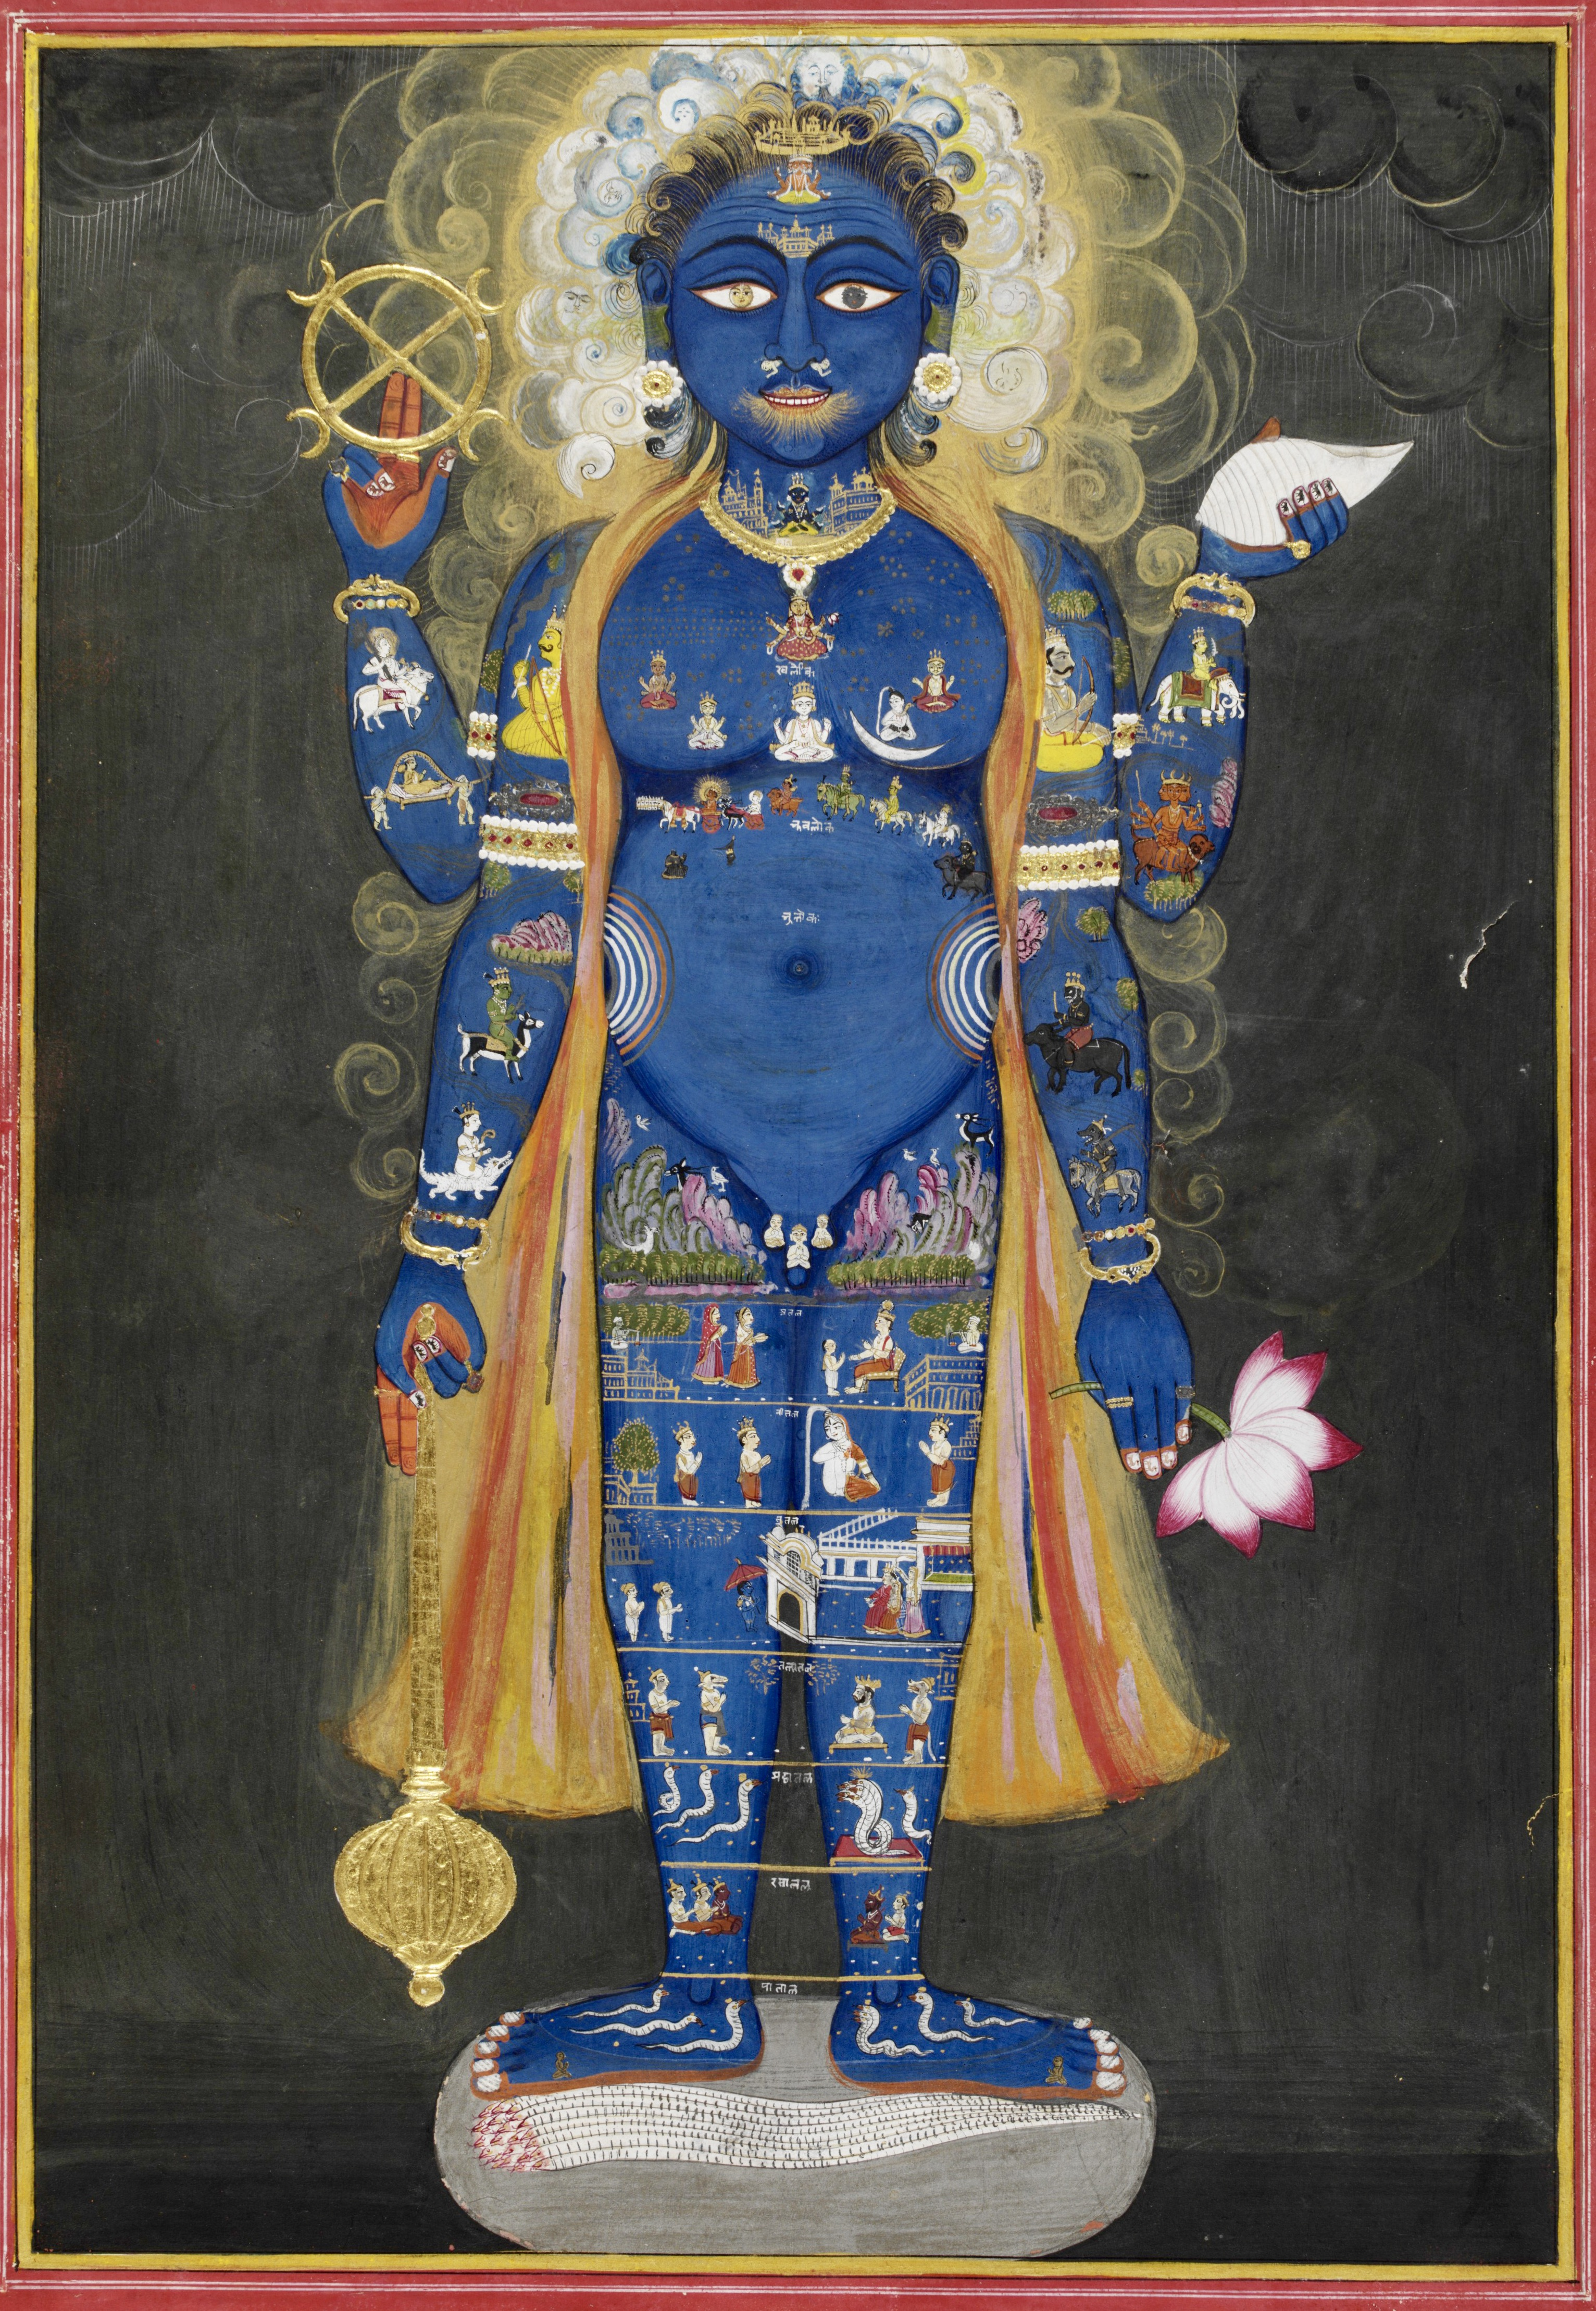
\includegraphics[width=1\textwidth]{pics/Vishnu_Vishvarupa_cropped.jpg}
	\caption{Viṣṇu Viśvarūpa, India, Rajasthan, Jaipur, ca. 1800–1820, Opaque watercolor and gold on paper, 38.5 × 28 cm, Victoria and Albert Museum, London, Given by Mrs. Gerald Clark.}
	\label{fig1}
      \end{figure}
\clearpage
  \begin{figure}[ht]
	\centering
  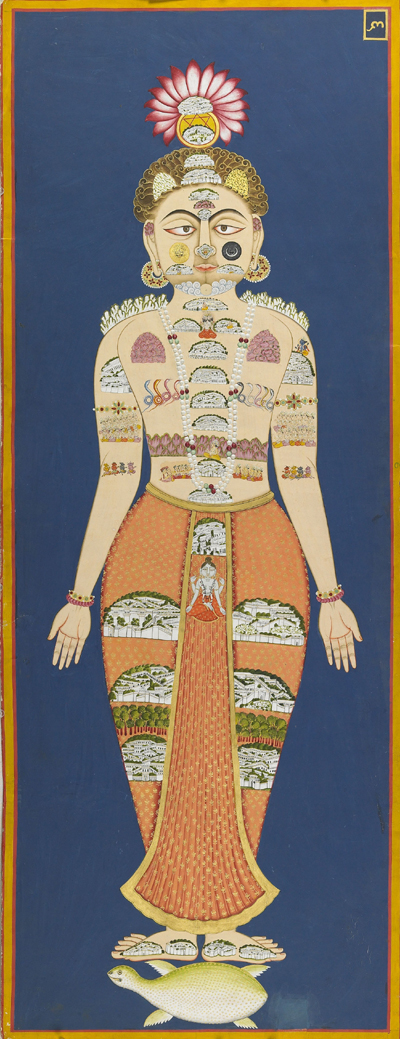
\includegraphics[width=0.5\textwidth]{pics/The_Equivalence_of_Self_and_Universe_(detail),_folio_6_from_the_Siddha_Siddhanta_Paddhati,_(Bulaki),_1824_(Samvat_1881);_122_x_46_cm._Mehrangarh_Museum_Trust..jpg}
	\caption{The Equivalence of Self and Universe (detail), folio 6 from the \textit{Siddhasiddhāntapaddhati} (Bulaki), India, Rajasthan, Jodhpur, 1824 (Samvat 1881), 122 x 46 cm, RJS 2378, Mehragarh Museum Trust.}
	\label{fig2}
      \end{figure}
      % \end{landscape}


\chapter{Bibliography}
 \label{sec:bibli}
   \clearpage
\newpage 
\thispagestyle{empty}
\quad  \addtocounter{page}{-1}

\printbibliography[heading=subbibintoc, title=Consulted Manuscripts, keyword=codex]

\printbibliography[heading=subbibintoc, title=Printed Editions, keyword=printsource]

\printbibliography[heading=subbibintoc, title=Secondary Literature, keyword=seclit]

\printbibliography[heading=subbibintoc, title=Online Sources, keyword=onlinesource]

\end{document}


